\documentclass[twoside]{book}

% Packages required by doxygen
\usepackage{calc}
\usepackage{doxygen}
\usepackage{graphicx}
\usepackage[utf8]{inputenc}
\usepackage{makeidx}
\usepackage{multicol}
\usepackage{multirow}
\usepackage{textcomp}
\usepackage[table]{xcolor}

% Font selection
\usepackage[T1]{fontenc}
\usepackage{mathptmx}
\usepackage[scaled=.90]{helvet}
\usepackage{courier}
\usepackage{amssymb}
\usepackage{sectsty}
\renewcommand{\familydefault}{\sfdefault}
\allsectionsfont{%
  \fontseries{bc}\selectfont%
  \color{darkgray}%
}
\renewcommand{\DoxyLabelFont}{%
  \fontseries{bc}\selectfont%
  \color{darkgray}%
}

% Page & text layout
\usepackage{geometry}
\geometry{%
  a4paper,%
  top=2.5cm,%
  bottom=2.5cm,%
  left=2.5cm,%
  right=2.5cm%
}
\tolerance=750
\hfuzz=15pt
\hbadness=750
\setlength{\emergencystretch}{15pt}
\setlength{\parindent}{0cm}
\setlength{\parskip}{0.2cm}
\makeatletter
\renewcommand{\paragraph}{%
  \@startsection{paragraph}{4}{0ex}{-1.0ex}{1.0ex}{%
    \normalfont\normalsize\bfseries\SS@parafont%
  }%
}
\renewcommand{\subparagraph}{%
  \@startsection{subparagraph}{5}{0ex}{-1.0ex}{1.0ex}{%
    \normalfont\normalsize\bfseries\SS@subparafont%
  }%
}
\makeatother

% Headers & footers
\usepackage{fancyhdr}
\pagestyle{fancyplain}
\fancyhead[LE]{\fancyplain{}{\bfseries\thepage}}
\fancyhead[CE]{\fancyplain{}{}}
\fancyhead[RE]{\fancyplain{}{\bfseries\leftmark}}
\fancyhead[LO]{\fancyplain{}{\bfseries\rightmark}}
\fancyhead[CO]{\fancyplain{}{}}
\fancyhead[RO]{\fancyplain{}{\bfseries\thepage}}
\fancyfoot[LE]{\fancyplain{}{}}
\fancyfoot[CE]{\fancyplain{}{}}
\fancyfoot[RE]{\fancyplain{}{\bfseries\scriptsize Generated on Thu Aug 13 2015 13\-:50\-:51 for Buildm\-Learn Toolkit for Android by Doxygen }}
\fancyfoot[LO]{\fancyplain{}{\bfseries\scriptsize Generated on Thu Aug 13 2015 13\-:50\-:51 for Buildm\-Learn Toolkit for Android by Doxygen }}
\fancyfoot[CO]{\fancyplain{}{}}
\fancyfoot[RO]{\fancyplain{}{}}
\renewcommand{\footrulewidth}{0.4pt}
\renewcommand{\chaptermark}[1]{%
  \markboth{#1}{}%
}
\renewcommand{\sectionmark}[1]{%
  \markright{\thesection\ #1}%
}

% Indices & bibliography
\usepackage{natbib}
\usepackage[titles]{tocloft}
\setcounter{tocdepth}{3}
\setcounter{secnumdepth}{5}
\makeindex

% Hyperlinks (required, but should be loaded last)
\usepackage{ifpdf}
\ifpdf
  \usepackage[pdftex,pagebackref=true]{hyperref}
\else
  \usepackage[ps2pdf,pagebackref=true]{hyperref}
\fi
\hypersetup{%
  colorlinks=true,%
  linkcolor=blue,%
  citecolor=blue,%
  unicode%
}

% Custom commands
\newcommand{\clearemptydoublepage}{%
  \newpage{\pagestyle{empty}\cleardoublepage}%
}


%===== C O N T E N T S =====

\begin{document}

% Titlepage & ToC
\hypersetup{pageanchor=false}
\pagenumbering{roman}
\begin{titlepage}
\vspace*{7cm}
\begin{center}%
{\Large Buildm\-Learn Toolkit for Android \\[1ex]\large 1.\-0.\-0 }\\
\vspace*{1cm}
{\large Generated by Doxygen 1.8.6}\\
\vspace*{0.5cm}
{\small Thu Aug 13 2015 13:50:51}\\
\end{center}
\end{titlepage}
\clearemptydoublepage
\tableofcontents
\clearemptydoublepage
\pagenumbering{arabic}
\hypersetup{pageanchor=true}

%--- Begin generated contents ---
\chapter{Namespace Index}
\section{Packages}
Here are the packages with brief descriptions (if available)\-:\begin{DoxyCompactList}
\item\contentsline{section}{\hyperlink{namespaceorg}{org} }{\pageref{db/d96/namespaceorg}}{}
\item\contentsline{section}{\hyperlink{namespaceorg_1_1buildmlearn}{org.\-buildmlearn} }{\pageref{d7/d90/namespaceorg_1_1buildmlearn}}{}
\item\contentsline{section}{\hyperlink{namespaceorg_1_1buildmlearn_1_1toolkit}{org.\-buildmlearn.\-toolkit} }{\pageref{d1/dcf/namespaceorg_1_1buildmlearn_1_1toolkit}}{}
\item\contentsline{section}{\hyperlink{namespaceorg_1_1buildmlearn_1_1toolkit_1_1activity}{org.\-buildmlearn.\-toolkit.\-activity} }{\pageref{d8/d88/namespaceorg_1_1buildmlearn_1_1toolkit_1_1activity}}{}
\item\contentsline{section}{\hyperlink{namespaceorg_1_1buildmlearn_1_1toolkit_1_1adapter}{org.\-buildmlearn.\-toolkit.\-adapter} }{\pageref{df/d2c/namespaceorg_1_1buildmlearn_1_1toolkit_1_1adapter}}{}
\item\contentsline{section}{\hyperlink{namespaceorg_1_1buildmlearn_1_1toolkit_1_1constant}{org.\-buildmlearn.\-toolkit.\-constant} }{\pageref{d7/d81/namespaceorg_1_1buildmlearn_1_1toolkit_1_1constant}}{}
\item\contentsline{section}{\hyperlink{namespaceorg_1_1buildmlearn_1_1toolkit_1_1flashcardtemplate}{org.\-buildmlearn.\-toolkit.\-flashcardtemplate} }{\pageref{df/d35/namespaceorg_1_1buildmlearn_1_1toolkit_1_1flashcardtemplate}}{}
\item\contentsline{section}{\hyperlink{namespaceorg_1_1buildmlearn_1_1toolkit_1_1fragment}{org.\-buildmlearn.\-toolkit.\-fragment} }{\pageref{df/d80/namespaceorg_1_1buildmlearn_1_1toolkit_1_1fragment}}{}
\item\contentsline{section}{\hyperlink{namespaceorg_1_1buildmlearn_1_1toolkit_1_1infotemplate}{org.\-buildmlearn.\-toolkit.\-infotemplate} }{\pageref{de/d1c/namespaceorg_1_1buildmlearn_1_1toolkit_1_1infotemplate}}{}
\item\contentsline{section}{\hyperlink{namespaceorg_1_1buildmlearn_1_1toolkit_1_1learnspelling}{org.\-buildmlearn.\-toolkit.\-learnspelling} }{\pageref{d1/d76/namespaceorg_1_1buildmlearn_1_1toolkit_1_1learnspelling}}{}
\item\contentsline{section}{\hyperlink{namespaceorg_1_1buildmlearn_1_1toolkit_1_1model}{org.\-buildmlearn.\-toolkit.\-model} }{\pageref{d6/da5/namespaceorg_1_1buildmlearn_1_1toolkit_1_1model}}{}
\item\contentsline{section}{\hyperlink{namespaceorg_1_1buildmlearn_1_1toolkit_1_1quiztemplate}{org.\-buildmlearn.\-toolkit.\-quiztemplate} }{\pageref{de/ddc/namespaceorg_1_1buildmlearn_1_1toolkit_1_1quiztemplate}}{}
\item\contentsline{section}{\hyperlink{namespaceorg_1_1buildmlearn_1_1toolkit_1_1simulator}{org.\-buildmlearn.\-toolkit.\-simulator} }{\pageref{d6/da8/namespaceorg_1_1buildmlearn_1_1toolkit_1_1simulator}}{}
\item\contentsline{section}{\hyperlink{namespaceorg_1_1buildmlearn_1_1toolkit_1_1templates}{org.\-buildmlearn.\-toolkit.\-templates} }{\pageref{d4/d17/namespaceorg_1_1buildmlearn_1_1toolkit_1_1templates}}{}
\item\contentsline{section}{\hyperlink{namespaceorg_1_1buildmlearn_1_1toolkit_1_1utilities}{org.\-buildmlearn.\-toolkit.\-utilities} }{\pageref{de/d09/namespaceorg_1_1buildmlearn_1_1toolkit_1_1utilities}}{}
\item\contentsline{section}{\hyperlink{namespaceorg_1_1buildmlearn_1_1toolkit_1_1views}{org.\-buildmlearn.\-toolkit.\-views} }{\pageref{d5/d61/namespaceorg_1_1buildmlearn_1_1toolkit_1_1views}}{}
\end{DoxyCompactList}

\chapter{Hierarchical Index}
\section{Class Hierarchy}
This inheritance list is sorted roughly, but not completely, alphabetically\-:\begin{DoxyCompactList}
\item \contentsline{section}{org.\-buildmlearn.\-toolkit.\-utilities.\-Alias}{\pageref{da/d11/classorg_1_1buildmlearn_1_1toolkit_1_1utilities_1_1Alias}}{}
\item \contentsline{section}{org.\-buildmlearn.\-toolkit.\-constant.\-Constants}{\pageref{de/d90/classorg_1_1buildmlearn_1_1toolkit_1_1constant_1_1Constants}}{}
\item \contentsline{section}{org.\-buildmlearn.\-toolkit.\-learnspelling.\-Data\-Manager}{\pageref{d9/db9/classorg_1_1buildmlearn_1_1toolkit_1_1learnspelling_1_1DataManager}}{}
\item \contentsline{section}{org.\-buildmlearn.\-toolkit.\-utilities.\-File\-Utils}{\pageref{d5/df1/classorg_1_1buildmlearn_1_1toolkit_1_1utilities_1_1FileUtils}}{}
\item \contentsline{section}{org.\-buildmlearn.\-toolkit.\-flashcardtemplate.\-Flash\-Model}{\pageref{da/da9/classorg_1_1buildmlearn_1_1toolkit_1_1flashcardtemplate_1_1FlashModel}}{}
\item \contentsline{section}{org.\-buildmlearn.\-toolkit.\-flashcardtemplate.\-Global\-Data}{\pageref{d1/d2a/classorg_1_1buildmlearn_1_1toolkit_1_1flashcardtemplate_1_1GlobalData}}{}
\item \contentsline{section}{org.\-buildmlearn.\-toolkit.\-infotemplate.\-Global\-Data}{\pageref{d1/d93/classorg_1_1buildmlearn_1_1toolkit_1_1infotemplate_1_1GlobalData}}{}
\item \contentsline{section}{org.\-buildmlearn.\-toolkit.\-quiztemplate.\-Global\-Data}{\pageref{d9/d00/classorg_1_1buildmlearn_1_1toolkit_1_1quiztemplate_1_1GlobalData}}{}
\item \contentsline{section}{org.\-buildmlearn.\-toolkit.\-templates.\-Flash\-Card\-Adapter.\-Holder}{\pageref{d7/d2d/classorg_1_1buildmlearn_1_1toolkit_1_1templates_1_1FlashCardAdapter_1_1Holder}}{}
\item \contentsline{section}{org.\-buildmlearn.\-toolkit.\-templates.\-Quiz\-Adapter.\-Holder}{\pageref{d5/dff/classorg_1_1buildmlearn_1_1toolkit_1_1templates_1_1QuizAdapter_1_1Holder}}{}
\item \contentsline{section}{org.\-buildmlearn.\-toolkit.\-infotemplate.\-Info\-Model}{\pageref{d8/d7e/classorg_1_1buildmlearn_1_1toolkit_1_1infotemplate_1_1InfoModel}}{}
\item \contentsline{section}{org.\-buildmlearn.\-toolkit.\-templates.\-Info\-Adapter.\-Info\-Template\-Holder}{\pageref{d7/d28/classorg_1_1buildmlearn_1_1toolkit_1_1templates_1_1InfoAdapter_1_1InfoTemplateHolder}}{}
\item \contentsline{section}{org.\-buildmlearn.\-toolkit.\-utilities.\-Keystore}{\pageref{dd/de3/classorg_1_1buildmlearn_1_1toolkit_1_1utilities_1_1Keystore}}{}
\item \contentsline{section}{org.\-buildmlearn.\-toolkit.\-model.\-Key\-Store\-Details}{\pageref{d4/de6/classorg_1_1buildmlearn_1_1toolkit_1_1model_1_1KeyStoreDetails}}{}
\item \contentsline{section}{org.\-buildmlearn.\-toolkit.\-templates.\-Learn\-Spelling\-Adapter.\-Learn\-Spelling\-Holder}{\pageref{d7/dea/classorg_1_1buildmlearn_1_1toolkit_1_1templates_1_1LearnSpellingAdapter_1_1LearnSpellingHolder}}{}
\item \contentsline{section}{org.\-buildmlearn.\-toolkit.\-fragment.\-Navigation\-Drawer\-Fragment.\-Navigation\-Drawer\-Callbacks}{\pageref{d5/dee/interfaceorg_1_1buildmlearn_1_1toolkit_1_1fragment_1_1NavigationDrawerFragment_1_1NavigationDrawerCallbacks}}{}
\begin{DoxyCompactList}
\item \contentsline{section}{org.\-buildmlearn.\-toolkit.\-activity.\-Home\-Activity}{\pageref{d6/d8d/classorg_1_1buildmlearn_1_1toolkit_1_1activity_1_1HomeActivity}}{}
\end{DoxyCompactList}
\item On\-Init\-Listener\begin{DoxyCompactList}
\item \contentsline{section}{org.\-buildmlearn.\-toolkit.\-learnspelling.\-Spelling\-Activity}{\pageref{d5/dbc/classorg_1_1buildmlearn_1_1toolkit_1_1learnspelling_1_1SpellingActivity}}{}
\end{DoxyCompactList}
\item On\-Item\-Click\-Listener\begin{DoxyCompactList}
\item \contentsline{section}{org.\-buildmlearn.\-toolkit.\-fragment.\-Load\-Project\-Fragment}{\pageref{d9/df8/classorg_1_1buildmlearn_1_1toolkit_1_1fragment_1_1LoadProjectFragment}}{}
\end{DoxyCompactList}
\item \contentsline{section}{org.\-buildmlearn.\-toolkit.\-utilities.\-Signer\-Thread.\-On\-Sign\-Complete}{\pageref{dd/df0/interfaceorg_1_1buildmlearn_1_1toolkit_1_1utilities_1_1SignerThread_1_1OnSignComplete}}{}
\item \contentsline{section}{org.\-buildmlearn.\-toolkit.\-adapter.\-Saved\-Project\-Adapter.\-Project\-Holder}{\pageref{d1/d04/classorg_1_1buildmlearn_1_1toolkit_1_1adapter_1_1SavedProjectAdapter_1_1ProjectHolder}}{}
\item \contentsline{section}{org.\-buildmlearn.\-toolkit.\-quiztemplate.\-Question\-Model}{\pageref{d6/de2/classorg_1_1buildmlearn_1_1toolkit_1_1quiztemplate_1_1QuestionModel}}{}
\item \contentsline{section}{org.\-buildmlearn.\-toolkit.\-model.\-Saved\-Project}{\pageref{db/d7b/classorg_1_1buildmlearn_1_1toolkit_1_1model_1_1SavedProject}}{}
\item \contentsline{section}{org.\-buildmlearn.\-toolkit.\-model.\-Section}{\pageref{db/d99/enumorg_1_1buildmlearn_1_1toolkit_1_1model_1_1Section}}{}
\item \contentsline{section}{org.\-buildmlearn.\-toolkit.\-model.\-Template}{\pageref{da/dbd/enumorg_1_1buildmlearn_1_1toolkit_1_1model_1_1Template}}{}
\item Thread\begin{DoxyCompactList}
\item \contentsline{section}{org.\-buildmlearn.\-toolkit.\-utilities.\-Signer\-Thread}{\pageref{d0/d6a/classorg_1_1buildmlearn_1_1toolkit_1_1utilities_1_1SignerThread}}{}
\end{DoxyCompactList}
\item \contentsline{section}{org.\-buildmlearn.\-toolkit.\-model.\-Tutorial}{\pageref{d9/d22/enumorg_1_1buildmlearn_1_1toolkit_1_1model_1_1Tutorial}}{}
\item \contentsline{section}{org.\-buildmlearn.\-toolkit.\-infotemplate.\-Info\-List\-Adapter.\-View\-Holder}{\pageref{d3/d3b/classorg_1_1buildmlearn_1_1toolkit_1_1infotemplate_1_1InfoListAdapter_1_1ViewHolder}}{}
\item \contentsline{section}{org.\-buildmlearn.\-toolkit.\-learnspelling.\-Word\-Model}{\pageref{d3/d6b/classorg_1_1buildmlearn_1_1toolkit_1_1learnspelling_1_1WordModel}}{}
\item Activity\begin{DoxyCompactList}
\item \contentsline{section}{org.\-buildmlearn.\-toolkit.\-activity.\-Deep\-Linker\-Activity}{\pageref{d5/df3/classorg_1_1buildmlearn_1_1toolkit_1_1activity_1_1DeepLinkerActivity}}{}
\end{DoxyCompactList}
\item Animation\-Listener\begin{DoxyCompactList}
\item \contentsline{section}{org.\-buildmlearn.\-toolkit.\-flashcardtemplate.\-Main\-Fragment}{\pageref{d3/d86/classorg_1_1buildmlearn_1_1toolkit_1_1flashcardtemplate_1_1MainFragment}}{}
\end{DoxyCompactList}
\item App\-Compat\-Activity\begin{DoxyCompactList}
\item \contentsline{section}{org.\-buildmlearn.\-toolkit.\-activity.\-About\-Buildm\-Learn}{\pageref{d3/d5f/classorg_1_1buildmlearn_1_1toolkit_1_1activity_1_1AboutBuildmLearn}}{}
\item \contentsline{section}{org.\-buildmlearn.\-toolkit.\-activity.\-First\-Run\-Activity}{\pageref{d8/d00/classorg_1_1buildmlearn_1_1toolkit_1_1activity_1_1FirstRunActivity}}{}
\item \contentsline{section}{org.\-buildmlearn.\-toolkit.\-activity.\-Home\-Activity}{\pageref{d6/d8d/classorg_1_1buildmlearn_1_1toolkit_1_1activity_1_1HomeActivity}}{}
\item \contentsline{section}{org.\-buildmlearn.\-toolkit.\-activity.\-Template\-Activity}{\pageref{da/da2/classorg_1_1buildmlearn_1_1toolkit_1_1activity_1_1TemplateActivity}}{}
\item \contentsline{section}{org.\-buildmlearn.\-toolkit.\-activity.\-Template\-Editor}{\pageref{d9/dfb/classorg_1_1buildmlearn_1_1toolkit_1_1activity_1_1TemplateEditor}}{}
\item \contentsline{section}{org.\-buildmlearn.\-toolkit.\-activity.\-Tutorial\-Activity}{\pageref{df/dd9/classorg_1_1buildmlearn_1_1toolkit_1_1activity_1_1TutorialActivity}}{}
\item \contentsline{section}{org.\-buildmlearn.\-toolkit.\-simulator.\-Simulator}{\pageref{dc/d7c/classorg_1_1buildmlearn_1_1toolkit_1_1simulator_1_1Simulator}}{}
\end{DoxyCompactList}
\item Application\begin{DoxyCompactList}
\item \contentsline{section}{org.\-buildmlearn.\-toolkit.\-Toolkit\-Application}{\pageref{d2/dda/classorg_1_1buildmlearn_1_1toolkit_1_1ToolkitApplication}}{}
\end{DoxyCompactList}
\item Base\-Adapter\begin{DoxyCompactList}
\item \contentsline{section}{org.\-buildmlearn.\-toolkit.\-adapter.\-Navigation\-Drawer\-Menu\-Adapter}{\pageref{dd/db7/classorg_1_1buildmlearn_1_1toolkit_1_1adapter_1_1NavigationDrawerMenuAdapter}}{}
\item \contentsline{section}{org.\-buildmlearn.\-toolkit.\-adapter.\-Saved\-Project\-Adapter}{\pageref{d1/da6/classorg_1_1buildmlearn_1_1toolkit_1_1adapter_1_1SavedProjectAdapter}}{}
\item \contentsline{section}{org.\-buildmlearn.\-toolkit.\-adapter.\-Template\-Adapter}{\pageref{d1/d66/classorg_1_1buildmlearn_1_1toolkit_1_1adapter_1_1TemplateAdapter}}{}
\item \contentsline{section}{org.\-buildmlearn.\-toolkit.\-infotemplate.\-Info\-List\-Adapter}{\pageref{d4/d40/classorg_1_1buildmlearn_1_1toolkit_1_1infotemplate_1_1InfoListAdapter}}{}
\item \contentsline{section}{org.\-buildmlearn.\-toolkit.\-templates.\-Flash\-Card\-Adapter}{\pageref{dd/dc9/classorg_1_1buildmlearn_1_1toolkit_1_1templates_1_1FlashCardAdapter}}{}
\item \contentsline{section}{org.\-buildmlearn.\-toolkit.\-templates.\-Info\-Adapter}{\pageref{d7/d0d/classorg_1_1buildmlearn_1_1toolkit_1_1templates_1_1InfoAdapter}}{}
\item \contentsline{section}{org.\-buildmlearn.\-toolkit.\-templates.\-Learn\-Spelling\-Adapter}{\pageref{d3/daa/classorg_1_1buildmlearn_1_1toolkit_1_1templates_1_1LearnSpellingAdapter}}{}
\item \contentsline{section}{org.\-buildmlearn.\-toolkit.\-templates.\-Quiz\-Adapter}{\pageref{dd/dd7/classorg_1_1buildmlearn_1_1toolkit_1_1templates_1_1QuizAdapter}}{}
\end{DoxyCompactList}
\item Fragment\begin{DoxyCompactList}
\item \contentsline{section}{org.\-buildmlearn.\-toolkit.\-flashcardtemplate.\-Main\-Fragment}{\pageref{d3/d86/classorg_1_1buildmlearn_1_1toolkit_1_1flashcardtemplate_1_1MainFragment}}{}
\item \contentsline{section}{org.\-buildmlearn.\-toolkit.\-flashcardtemplate.\-Score\-Fragment}{\pageref{d1/d27/classorg_1_1buildmlearn_1_1toolkit_1_1flashcardtemplate_1_1ScoreFragment}}{}
\item \contentsline{section}{org.\-buildmlearn.\-toolkit.\-flashcardtemplate.\-Start\-Fragment}{\pageref{dd/d12/classorg_1_1buildmlearn_1_1toolkit_1_1flashcardtemplate_1_1StartFragment}}{}
\item \contentsline{section}{org.\-buildmlearn.\-toolkit.\-fragment.\-Home\-Fragment}{\pageref{d1/dfb/classorg_1_1buildmlearn_1_1toolkit_1_1fragment_1_1HomeFragment}}{}
\item \contentsline{section}{org.\-buildmlearn.\-toolkit.\-fragment.\-Load\-Project\-Fragment}{\pageref{d9/df8/classorg_1_1buildmlearn_1_1toolkit_1_1fragment_1_1LoadProjectFragment}}{}
\item \contentsline{section}{org.\-buildmlearn.\-toolkit.\-fragment.\-Navigation\-Drawer\-Fragment}{\pageref{d1/df1/classorg_1_1buildmlearn_1_1toolkit_1_1fragment_1_1NavigationDrawerFragment}}{}
\item \contentsline{section}{org.\-buildmlearn.\-toolkit.\-infotemplate.\-Detail\-View}{\pageref{d6/dde/classorg_1_1buildmlearn_1_1toolkit_1_1infotemplate_1_1DetailView}}{}
\item \contentsline{section}{org.\-buildmlearn.\-toolkit.\-learnspelling.\-Result\-Activity}{\pageref{d3/d40/classorg_1_1buildmlearn_1_1toolkit_1_1learnspelling_1_1ResultActivity}}{}
\item \contentsline{section}{org.\-buildmlearn.\-toolkit.\-learnspelling.\-Spelling\-Activity}{\pageref{d5/dbc/classorg_1_1buildmlearn_1_1toolkit_1_1learnspelling_1_1SpellingActivity}}{}
\item \contentsline{section}{org.\-buildmlearn.\-toolkit.\-learnspelling.\-Spelling\-Main\-Fragment}{\pageref{df/dff/classorg_1_1buildmlearn_1_1toolkit_1_1learnspelling_1_1SpellingMainFragment}}{}
\item \contentsline{section}{org.\-buildmlearn.\-toolkit.\-learnspelling.\-Word\-Info\-Activity}{\pageref{d1/d42/classorg_1_1buildmlearn_1_1toolkit_1_1learnspelling_1_1WordInfoActivity}}{}
\item \contentsline{section}{org.\-buildmlearn.\-toolkit.\-quiztemplate.\-Question\-Fragment}{\pageref{dd/dc1/classorg_1_1buildmlearn_1_1toolkit_1_1quiztemplate_1_1QuestionFragment}}{}
\item \contentsline{section}{org.\-buildmlearn.\-toolkit.\-quiztemplate.\-Score\-Fragment}{\pageref{d1/d71/classorg_1_1buildmlearn_1_1toolkit_1_1quiztemplate_1_1ScoreFragment}}{}
\item \contentsline{section}{org.\-buildmlearn.\-toolkit.\-quiztemplate.\-T\-F\-T\-Quiz\-Fragment}{\pageref{d8/d18/classorg_1_1buildmlearn_1_1toolkit_1_1quiztemplate_1_1TFTQuizFragment}}{}
\end{DoxyCompactList}
\item List\-Fragment\begin{DoxyCompactList}
\item \contentsline{section}{org.\-buildmlearn.\-toolkit.\-infotemplate.\-T\-F\-T\-Fragment}{\pageref{d3/dc0/classorg_1_1buildmlearn_1_1toolkit_1_1infotemplate_1_1TFTFragment}}{}
\end{DoxyCompactList}
\item Pager\-Adapter\begin{DoxyCompactList}
\item \contentsline{section}{org.\-buildmlearn.\-toolkit.\-adapter.\-Tutorial\-Adapter}{\pageref{de/d98/classorg_1_1buildmlearn_1_1toolkit_1_1adapter_1_1TutorialAdapter}}{}
\end{DoxyCompactList}
\item Preference\-Fragment\begin{DoxyCompactList}
\item \contentsline{section}{org.\-buildmlearn.\-toolkit.\-fragment.\-Settings\-Fragment}{\pageref{df/d0e/classorg_1_1buildmlearn_1_1toolkit_1_1fragment_1_1SettingsFragment}}{}
\end{DoxyCompactList}
\item Resource\-Adapter\begin{DoxyCompactList}
\item \contentsline{section}{org.\-buildmlearn.\-toolkit.\-utilities.\-Zip\-Signer\-App\-Resource\-Adapter}{\pageref{d5/ddf/classorg_1_1buildmlearn_1_1toolkit_1_1utilities_1_1ZipSignerAppResourceAdapter}}{}
\end{DoxyCompactList}
\item Serializable\begin{DoxyCompactList}
\item \contentsline{section}{org.\-buildmlearn.\-toolkit.\-model.\-Template\-Interface}{\pageref{de/dba/interfaceorg_1_1buildmlearn_1_1toolkit_1_1model_1_1TemplateInterface}}{}
\begin{DoxyCompactList}
\item \contentsline{section}{org.\-buildmlearn.\-toolkit.\-templates.\-Flash\-Template}{\pageref{d6/dbf/classorg_1_1buildmlearn_1_1toolkit_1_1templates_1_1FlashTemplate}}{}
\item \contentsline{section}{org.\-buildmlearn.\-toolkit.\-templates.\-Info\-Template}{\pageref{df/d53/classorg_1_1buildmlearn_1_1toolkit_1_1templates_1_1InfoTemplate}}{}
\item \contentsline{section}{org.\-buildmlearn.\-toolkit.\-templates.\-Learn\-Spelling\-Template}{\pageref{d7/dbc/classorg_1_1buildmlearn_1_1toolkit_1_1templates_1_1LearnSpellingTemplate}}{}
\item \contentsline{section}{org.\-buildmlearn.\-toolkit.\-templates.\-Quiz\-Template}{\pageref{da/d66/classorg_1_1buildmlearn_1_1toolkit_1_1templates_1_1QuizTemplate}}{}
\end{DoxyCompactList}
\item \contentsline{section}{org.\-buildmlearn.\-toolkit.\-templates.\-Flash\-Card\-Model}{\pageref{d6/d15/classorg_1_1buildmlearn_1_1toolkit_1_1templates_1_1FlashCardModel}}{}
\item \contentsline{section}{org.\-buildmlearn.\-toolkit.\-templates.\-Info\-Model}{\pageref{d8/d2b/classorg_1_1buildmlearn_1_1toolkit_1_1templates_1_1InfoModel}}{}
\item \contentsline{section}{org.\-buildmlearn.\-toolkit.\-templates.\-Learn\-Spelling\-Model}{\pageref{d3/d30/classorg_1_1buildmlearn_1_1toolkit_1_1templates_1_1LearnSpellingModel}}{}
\item \contentsline{section}{org.\-buildmlearn.\-toolkit.\-templates.\-Quiz\-Model}{\pageref{d5/d7e/classorg_1_1buildmlearn_1_1toolkit_1_1templates_1_1QuizModel}}{}
\end{DoxyCompactList}
\item Text\-View\begin{DoxyCompactList}
\item \contentsline{section}{org.\-buildmlearn.\-toolkit.\-views.\-Text\-View\-Plus}{\pageref{d7/d0b/classorg_1_1buildmlearn_1_1toolkit_1_1views_1_1TextViewPlus}}{}
\end{DoxyCompactList}
\end{DoxyCompactList}

\chapter{Class Index}
\section{Class List}
Here are the classes, structs, unions and interfaces with brief descriptions\-:\begin{DoxyCompactList}
\item\contentsline{section}{\hyperlink{classorg_1_1buildmlearn_1_1toolkit_1_1activity_1_1AboutBuildmLearn}{org.\-buildmlearn.\-toolkit.\-activity.\-About\-Buildm\-Learn} \\*Gives brief info about Buildm\-Learn community and toolkit }{\pageref{d3/d5f/classorg_1_1buildmlearn_1_1toolkit_1_1activity_1_1AboutBuildmLearn}}{}
\item\contentsline{section}{\hyperlink{classorg_1_1buildmlearn_1_1toolkit_1_1utilities_1_1Alias}{org.\-buildmlearn.\-toolkit.\-utilities.\-Alias} \\*Model class for storing \hyperlink{classorg_1_1buildmlearn_1_1toolkit_1_1utilities_1_1Alias}{Alias} data for keystore }{\pageref{da/d11/classorg_1_1buildmlearn_1_1toolkit_1_1utilities_1_1Alias}}{}
\item\contentsline{section}{\hyperlink{classorg_1_1buildmlearn_1_1toolkit_1_1constant_1_1Constants}{org.\-buildmlearn.\-toolkit.\-constant.\-Constants} \\*\hyperlink{classorg_1_1buildmlearn_1_1toolkit_1_1constant_1_1Constants}{Constants} related project directories, preferences and keys }{\pageref{de/d90/classorg_1_1buildmlearn_1_1toolkit_1_1constant_1_1Constants}}{}
\item\contentsline{section}{\hyperlink{classorg_1_1buildmlearn_1_1toolkit_1_1learnspelling_1_1DataManager}{org.\-buildmlearn.\-toolkit.\-learnspelling.\-Data\-Manager} \\*Simulator code for Learn Spelling Template }{\pageref{d9/db9/classorg_1_1buildmlearn_1_1toolkit_1_1learnspelling_1_1DataManager}}{}
\item\contentsline{section}{\hyperlink{classorg_1_1buildmlearn_1_1toolkit_1_1activity_1_1DeepLinkerActivity}{org.\-buildmlearn.\-toolkit.\-activity.\-Deep\-Linker\-Activity} \\*Activity responsible for handling files opened from file explorer }{\pageref{d5/df3/classorg_1_1buildmlearn_1_1toolkit_1_1activity_1_1DeepLinkerActivity}}{}
\item\contentsline{section}{\hyperlink{classorg_1_1buildmlearn_1_1toolkit_1_1infotemplate_1_1DetailView}{org.\-buildmlearn.\-toolkit.\-infotemplate.\-Detail\-View} \\*Simulator code for Info Template }{\pageref{d6/dde/classorg_1_1buildmlearn_1_1toolkit_1_1infotemplate_1_1DetailView}}{}
\item\contentsline{section}{\hyperlink{classorg_1_1buildmlearn_1_1toolkit_1_1utilities_1_1FileUtils}{org.\-buildmlearn.\-toolkit.\-utilities.\-File\-Utils} \\*Helper functions related to String manipulation }{\pageref{d5/df1/classorg_1_1buildmlearn_1_1toolkit_1_1utilities_1_1FileUtils}}{}
\item\contentsline{section}{\hyperlink{classorg_1_1buildmlearn_1_1toolkit_1_1activity_1_1FirstRunActivity}{org.\-buildmlearn.\-toolkit.\-activity.\-First\-Run\-Activity} \\*Shown on application first launch }{\pageref{d8/d00/classorg_1_1buildmlearn_1_1toolkit_1_1activity_1_1FirstRunActivity}}{}
\item\contentsline{section}{\hyperlink{classorg_1_1buildmlearn_1_1toolkit_1_1templates_1_1FlashCardAdapter}{org.\-buildmlearn.\-toolkit.\-templates.\-Flash\-Card\-Adapter} \\*Adapter for displaying Flash Card Template Editor data }{\pageref{dd/dc9/classorg_1_1buildmlearn_1_1toolkit_1_1templates_1_1FlashCardAdapter}}{}
\item\contentsline{section}{\hyperlink{classorg_1_1buildmlearn_1_1toolkit_1_1templates_1_1FlashCardModel}{org.\-buildmlearn.\-toolkit.\-templates.\-Flash\-Card\-Model} \\*Model class for Flash Card Template Editor data }{\pageref{d6/d15/classorg_1_1buildmlearn_1_1toolkit_1_1templates_1_1FlashCardModel}}{}
\item\contentsline{section}{\hyperlink{classorg_1_1buildmlearn_1_1toolkit_1_1flashcardtemplate_1_1FlashModel}{org.\-buildmlearn.\-toolkit.\-flashcardtemplate.\-Flash\-Model} \\*Simulator code for Flash Card Template }{\pageref{da/da9/classorg_1_1buildmlearn_1_1toolkit_1_1flashcardtemplate_1_1FlashModel}}{}
\item\contentsline{section}{\hyperlink{classorg_1_1buildmlearn_1_1toolkit_1_1templates_1_1FlashTemplate}{org.\-buildmlearn.\-toolkit.\-templates.\-Flash\-Template} \\*Flash Card template code implementing methods of Template\-Interface }{\pageref{d6/dbf/classorg_1_1buildmlearn_1_1toolkit_1_1templates_1_1FlashTemplate}}{}
\item\contentsline{section}{\hyperlink{classorg_1_1buildmlearn_1_1toolkit_1_1flashcardtemplate_1_1GlobalData}{org.\-buildmlearn.\-toolkit.\-flashcardtemplate.\-Global\-Data} \\*Simulator code for Flash Card Template }{\pageref{d1/d2a/classorg_1_1buildmlearn_1_1toolkit_1_1flashcardtemplate_1_1GlobalData}}{}
\item\contentsline{section}{\hyperlink{classorg_1_1buildmlearn_1_1toolkit_1_1infotemplate_1_1GlobalData}{org.\-buildmlearn.\-toolkit.\-infotemplate.\-Global\-Data} \\*Simulator code for Info Template }{\pageref{d1/d93/classorg_1_1buildmlearn_1_1toolkit_1_1infotemplate_1_1GlobalData}}{}
\item\contentsline{section}{\hyperlink{classorg_1_1buildmlearn_1_1toolkit_1_1quiztemplate_1_1GlobalData}{org.\-buildmlearn.\-toolkit.\-quiztemplate.\-Global\-Data} \\*Simulator code for Quiz Template }{\pageref{d9/d00/classorg_1_1buildmlearn_1_1toolkit_1_1quiztemplate_1_1GlobalData}}{}
\item\contentsline{section}{\hyperlink{classorg_1_1buildmlearn_1_1toolkit_1_1templates_1_1FlashCardAdapter_1_1Holder}{org.\-buildmlearn.\-toolkit.\-templates.\-Flash\-Card\-Adapter.\-Holder} }{\pageref{d7/d2d/classorg_1_1buildmlearn_1_1toolkit_1_1templates_1_1FlashCardAdapter_1_1Holder}}{}
\item\contentsline{section}{\hyperlink{classorg_1_1buildmlearn_1_1toolkit_1_1templates_1_1QuizAdapter_1_1Holder}{org.\-buildmlearn.\-toolkit.\-templates.\-Quiz\-Adapter.\-Holder} }{\pageref{d5/dff/classorg_1_1buildmlearn_1_1toolkit_1_1templates_1_1QuizAdapter_1_1Holder}}{}
\item\contentsline{section}{\hyperlink{classorg_1_1buildmlearn_1_1toolkit_1_1activity_1_1HomeActivity}{org.\-buildmlearn.\-toolkit.\-activity.\-Home\-Activity} \\*Home screen of the application containg all the menus and settings }{\pageref{d6/d8d/classorg_1_1buildmlearn_1_1toolkit_1_1activity_1_1HomeActivity}}{}
\item\contentsline{section}{\hyperlink{classorg_1_1buildmlearn_1_1toolkit_1_1fragment_1_1HomeFragment}{org.\-buildmlearn.\-toolkit.\-fragment.\-Home\-Fragment} \\*Fragment displayed on the home screen }{\pageref{d1/dfb/classorg_1_1buildmlearn_1_1toolkit_1_1fragment_1_1HomeFragment}}{}
\item\contentsline{section}{\hyperlink{classorg_1_1buildmlearn_1_1toolkit_1_1templates_1_1InfoAdapter}{org.\-buildmlearn.\-toolkit.\-templates.\-Info\-Adapter} \\*Adapter for displaying Info Template Editor data }{\pageref{d7/d0d/classorg_1_1buildmlearn_1_1toolkit_1_1templates_1_1InfoAdapter}}{}
\item\contentsline{section}{\hyperlink{classorg_1_1buildmlearn_1_1toolkit_1_1infotemplate_1_1InfoListAdapter}{org.\-buildmlearn.\-toolkit.\-infotemplate.\-Info\-List\-Adapter} \\*Simulator code for Info Template }{\pageref{d4/d40/classorg_1_1buildmlearn_1_1toolkit_1_1infotemplate_1_1InfoListAdapter}}{}
\item\contentsline{section}{\hyperlink{classorg_1_1buildmlearn_1_1toolkit_1_1infotemplate_1_1InfoModel}{org.\-buildmlearn.\-toolkit.\-infotemplate.\-Info\-Model} \\*Simulator code for Info Template }{\pageref{d8/d7e/classorg_1_1buildmlearn_1_1toolkit_1_1infotemplate_1_1InfoModel}}{}
\item\contentsline{section}{\hyperlink{classorg_1_1buildmlearn_1_1toolkit_1_1templates_1_1InfoModel}{org.\-buildmlearn.\-toolkit.\-templates.\-Info\-Model} \\*Model class for Info Template Editor data }{\pageref{d8/d2b/classorg_1_1buildmlearn_1_1toolkit_1_1templates_1_1InfoModel}}{}
\item\contentsline{section}{\hyperlink{classorg_1_1buildmlearn_1_1toolkit_1_1templates_1_1InfoTemplate}{org.\-buildmlearn.\-toolkit.\-templates.\-Info\-Template} \\*Info template code implementing methods of Template\-Interface }{\pageref{df/d53/classorg_1_1buildmlearn_1_1toolkit_1_1templates_1_1InfoTemplate}}{}
\item\contentsline{section}{\hyperlink{classorg_1_1buildmlearn_1_1toolkit_1_1templates_1_1InfoAdapter_1_1InfoTemplateHolder}{org.\-buildmlearn.\-toolkit.\-templates.\-Info\-Adapter.\-Info\-Template\-Holder} }{\pageref{d7/d28/classorg_1_1buildmlearn_1_1toolkit_1_1templates_1_1InfoAdapter_1_1InfoTemplateHolder}}{}
\item\contentsline{section}{\hyperlink{classorg_1_1buildmlearn_1_1toolkit_1_1utilities_1_1Keystore}{org.\-buildmlearn.\-toolkit.\-utilities.\-Keystore} \\*Model class for storing \hyperlink{classorg_1_1buildmlearn_1_1toolkit_1_1utilities_1_1Keystore}{Keystore} details }{\pageref{dd/de3/classorg_1_1buildmlearn_1_1toolkit_1_1utilities_1_1Keystore}}{}
\item\contentsline{section}{\hyperlink{classorg_1_1buildmlearn_1_1toolkit_1_1model_1_1KeyStoreDetails}{org.\-buildmlearn.\-toolkit.\-model.\-Key\-Store\-Details} \\*Model class for holding the details of keystore file }{\pageref{d4/de6/classorg_1_1buildmlearn_1_1toolkit_1_1model_1_1KeyStoreDetails}}{}
\item\contentsline{section}{\hyperlink{classorg_1_1buildmlearn_1_1toolkit_1_1templates_1_1LearnSpellingAdapter}{org.\-buildmlearn.\-toolkit.\-templates.\-Learn\-Spelling\-Adapter} \\*Adapter for displaying Learn Spelling Template Editor data }{\pageref{d3/daa/classorg_1_1buildmlearn_1_1toolkit_1_1templates_1_1LearnSpellingAdapter}}{}
\item\contentsline{section}{\hyperlink{classorg_1_1buildmlearn_1_1toolkit_1_1templates_1_1LearnSpellingAdapter_1_1LearnSpellingHolder}{org.\-buildmlearn.\-toolkit.\-templates.\-Learn\-Spelling\-Adapter.\-Learn\-Spelling\-Holder} }{\pageref{d7/dea/classorg_1_1buildmlearn_1_1toolkit_1_1templates_1_1LearnSpellingAdapter_1_1LearnSpellingHolder}}{}
\item\contentsline{section}{\hyperlink{classorg_1_1buildmlearn_1_1toolkit_1_1templates_1_1LearnSpellingModel}{org.\-buildmlearn.\-toolkit.\-templates.\-Learn\-Spelling\-Model} \\*Model class for Learn Spelling Template Editor data }{\pageref{d3/d30/classorg_1_1buildmlearn_1_1toolkit_1_1templates_1_1LearnSpellingModel}}{}
\item\contentsline{section}{\hyperlink{classorg_1_1buildmlearn_1_1toolkit_1_1templates_1_1LearnSpellingTemplate}{org.\-buildmlearn.\-toolkit.\-templates.\-Learn\-Spelling\-Template} \\*Learn Spelling template code implementing methods of Template\-Interface }{\pageref{d7/dbc/classorg_1_1buildmlearn_1_1toolkit_1_1templates_1_1LearnSpellingTemplate}}{}
\item\contentsline{section}{\hyperlink{classorg_1_1buildmlearn_1_1toolkit_1_1fragment_1_1LoadProjectFragment}{org.\-buildmlearn.\-toolkit.\-fragment.\-Load\-Project\-Fragment} \\*Fragment used for loading existing projects into a list }{\pageref{d9/df8/classorg_1_1buildmlearn_1_1toolkit_1_1fragment_1_1LoadProjectFragment}}{}
\item\contentsline{section}{\hyperlink{classorg_1_1buildmlearn_1_1toolkit_1_1flashcardtemplate_1_1MainFragment}{org.\-buildmlearn.\-toolkit.\-flashcardtemplate.\-Main\-Fragment} \\*Simulator code for Flash Card Template }{\pageref{d3/d86/classorg_1_1buildmlearn_1_1toolkit_1_1flashcardtemplate_1_1MainFragment}}{}
\item\contentsline{section}{\hyperlink{interfaceorg_1_1buildmlearn_1_1toolkit_1_1fragment_1_1NavigationDrawerFragment_1_1NavigationDrawerCallbacks}{org.\-buildmlearn.\-toolkit.\-fragment.\-Navigation\-Drawer\-Fragment.\-Navigation\-Drawer\-Callbacks} }{\pageref{d5/dee/interfaceorg_1_1buildmlearn_1_1toolkit_1_1fragment_1_1NavigationDrawerFragment_1_1NavigationDrawerCallbacks}}{}
\item\contentsline{section}{\hyperlink{classorg_1_1buildmlearn_1_1toolkit_1_1fragment_1_1NavigationDrawerFragment}{org.\-buildmlearn.\-toolkit.\-fragment.\-Navigation\-Drawer\-Fragment} }{\pageref{d1/df1/classorg_1_1buildmlearn_1_1toolkit_1_1fragment_1_1NavigationDrawerFragment}}{}
\item\contentsline{section}{\hyperlink{classorg_1_1buildmlearn_1_1toolkit_1_1adapter_1_1NavigationDrawerMenuAdapter}{org.\-buildmlearn.\-toolkit.\-adapter.\-Navigation\-Drawer\-Menu\-Adapter} \\*Adapter used for showing menus in the side panel }{\pageref{dd/db7/classorg_1_1buildmlearn_1_1toolkit_1_1adapter_1_1NavigationDrawerMenuAdapter}}{}
\item\contentsline{section}{\hyperlink{interfaceorg_1_1buildmlearn_1_1toolkit_1_1utilities_1_1SignerThread_1_1OnSignComplete}{org.\-buildmlearn.\-toolkit.\-utilities.\-Signer\-Thread.\-On\-Sign\-Complete} }{\pageref{dd/df0/interfaceorg_1_1buildmlearn_1_1toolkit_1_1utilities_1_1SignerThread_1_1OnSignComplete}}{}
\item\contentsline{section}{\hyperlink{classorg_1_1buildmlearn_1_1toolkit_1_1adapter_1_1SavedProjectAdapter_1_1ProjectHolder}{org.\-buildmlearn.\-toolkit.\-adapter.\-Saved\-Project\-Adapter.\-Project\-Holder} }{\pageref{d1/d04/classorg_1_1buildmlearn_1_1toolkit_1_1adapter_1_1SavedProjectAdapter_1_1ProjectHolder}}{}
\item\contentsline{section}{\hyperlink{classorg_1_1buildmlearn_1_1toolkit_1_1quiztemplate_1_1QuestionFragment}{org.\-buildmlearn.\-toolkit.\-quiztemplate.\-Question\-Fragment} \\*Simulator code for Quiz Template }{\pageref{dd/dc1/classorg_1_1buildmlearn_1_1toolkit_1_1quiztemplate_1_1QuestionFragment}}{}
\item\contentsline{section}{\hyperlink{classorg_1_1buildmlearn_1_1toolkit_1_1quiztemplate_1_1QuestionModel}{org.\-buildmlearn.\-toolkit.\-quiztemplate.\-Question\-Model} \\*Simulator code for Quiz Template }{\pageref{d6/de2/classorg_1_1buildmlearn_1_1toolkit_1_1quiztemplate_1_1QuestionModel}}{}
\item\contentsline{section}{\hyperlink{classorg_1_1buildmlearn_1_1toolkit_1_1templates_1_1QuizAdapter}{org.\-buildmlearn.\-toolkit.\-templates.\-Quiz\-Adapter} \\*Adapter for displaying Quiz Template Editor data }{\pageref{dd/dd7/classorg_1_1buildmlearn_1_1toolkit_1_1templates_1_1QuizAdapter}}{}
\item\contentsline{section}{\hyperlink{classorg_1_1buildmlearn_1_1toolkit_1_1templates_1_1QuizModel}{org.\-buildmlearn.\-toolkit.\-templates.\-Quiz\-Model} \\*Model class for Quiz Template Editor data }{\pageref{d5/d7e/classorg_1_1buildmlearn_1_1toolkit_1_1templates_1_1QuizModel}}{}
\item\contentsline{section}{\hyperlink{classorg_1_1buildmlearn_1_1toolkit_1_1templates_1_1QuizTemplate}{org.\-buildmlearn.\-toolkit.\-templates.\-Quiz\-Template} \\*Quiz template code implementing methods of Template\-Interface }{\pageref{da/d66/classorg_1_1buildmlearn_1_1toolkit_1_1templates_1_1QuizTemplate}}{}
\item\contentsline{section}{\hyperlink{classorg_1_1buildmlearn_1_1toolkit_1_1learnspelling_1_1ResultActivity}{org.\-buildmlearn.\-toolkit.\-learnspelling.\-Result\-Activity} \\*Simulator code for Learn Spelling Template }{\pageref{d3/d40/classorg_1_1buildmlearn_1_1toolkit_1_1learnspelling_1_1ResultActivity}}{}
\item\contentsline{section}{\hyperlink{classorg_1_1buildmlearn_1_1toolkit_1_1model_1_1SavedProject}{org.\-buildmlearn.\-toolkit.\-model.\-Saved\-Project} \\*Model class for holding the details of a Saved File }{\pageref{db/d7b/classorg_1_1buildmlearn_1_1toolkit_1_1model_1_1SavedProject}}{}
\item\contentsline{section}{\hyperlink{classorg_1_1buildmlearn_1_1toolkit_1_1adapter_1_1SavedProjectAdapter}{org.\-buildmlearn.\-toolkit.\-adapter.\-Saved\-Project\-Adapter} \\*Adapter used for showing saved projects in a list }{\pageref{d1/da6/classorg_1_1buildmlearn_1_1toolkit_1_1adapter_1_1SavedProjectAdapter}}{}
\item\contentsline{section}{\hyperlink{classorg_1_1buildmlearn_1_1toolkit_1_1quiztemplate_1_1ScoreFragment}{org.\-buildmlearn.\-toolkit.\-quiztemplate.\-Score\-Fragment} \\*Simulator code for Quiz Template }{\pageref{d1/d71/classorg_1_1buildmlearn_1_1toolkit_1_1quiztemplate_1_1ScoreFragment}}{}
\item\contentsline{section}{\hyperlink{classorg_1_1buildmlearn_1_1toolkit_1_1flashcardtemplate_1_1ScoreFragment}{org.\-buildmlearn.\-toolkit.\-flashcardtemplate.\-Score\-Fragment} \\*Simulator code for Flash Card Template }{\pageref{d1/d27/classorg_1_1buildmlearn_1_1toolkit_1_1flashcardtemplate_1_1ScoreFragment}}{}
\item\contentsline{section}{\hyperlink{enumorg_1_1buildmlearn_1_1toolkit_1_1model_1_1Section}{org.\-buildmlearn.\-toolkit.\-model.\-Section} \\*Enum for navigation drawer menus }{\pageref{db/d99/enumorg_1_1buildmlearn_1_1toolkit_1_1model_1_1Section}}{}
\item\contentsline{section}{\hyperlink{classorg_1_1buildmlearn_1_1toolkit_1_1fragment_1_1SettingsFragment}{org.\-buildmlearn.\-toolkit.\-fragment.\-Settings\-Fragment} }{\pageref{df/d0e/classorg_1_1buildmlearn_1_1toolkit_1_1fragment_1_1SettingsFragment}}{}
\item\contentsline{section}{\hyperlink{classorg_1_1buildmlearn_1_1toolkit_1_1utilities_1_1SignerThread}{org.\-buildmlearn.\-toolkit.\-utilities.\-Signer\-Thread} \\*Class for signing a unsigned apk file using a given keystore and credentials }{\pageref{d0/d6a/classorg_1_1buildmlearn_1_1toolkit_1_1utilities_1_1SignerThread}}{}
\item\contentsline{section}{\hyperlink{classorg_1_1buildmlearn_1_1toolkit_1_1simulator_1_1Simulator}{org.\-buildmlearn.\-toolkit.\-simulator.\-Simulator} \\*This activity acts as a placeholder for \hyperlink{classorg_1_1buildmlearn_1_1toolkit_1_1simulator_1_1Simulator}{Simulator} fragment. Contains a Nexus 6 frame in which the fragments are laodded }{\pageref{dc/d7c/classorg_1_1buildmlearn_1_1toolkit_1_1simulator_1_1Simulator}}{}
\item\contentsline{section}{\hyperlink{classorg_1_1buildmlearn_1_1toolkit_1_1learnspelling_1_1SpellingActivity}{org.\-buildmlearn.\-toolkit.\-learnspelling.\-Spelling\-Activity} \\*Simulator code for Learn Spelling Template }{\pageref{d5/dbc/classorg_1_1buildmlearn_1_1toolkit_1_1learnspelling_1_1SpellingActivity}}{}
\item\contentsline{section}{\hyperlink{classorg_1_1buildmlearn_1_1toolkit_1_1learnspelling_1_1SpellingMainFragment}{org.\-buildmlearn.\-toolkit.\-learnspelling.\-Spelling\-Main\-Fragment} \\*Simulator code for Learn Spelling Template }{\pageref{df/dff/classorg_1_1buildmlearn_1_1toolkit_1_1learnspelling_1_1SpellingMainFragment}}{}
\item\contentsline{section}{\hyperlink{classorg_1_1buildmlearn_1_1toolkit_1_1flashcardtemplate_1_1StartFragment}{org.\-buildmlearn.\-toolkit.\-flashcardtemplate.\-Start\-Fragment} \\*Simulator code for Flash Card Template }{\pageref{dd/d12/classorg_1_1buildmlearn_1_1toolkit_1_1flashcardtemplate_1_1StartFragment}}{}
\item\contentsline{section}{\hyperlink{enumorg_1_1buildmlearn_1_1toolkit_1_1model_1_1Template}{org.\-buildmlearn.\-toolkit.\-model.\-Template} \\*Enum for the templates that are included into toolkit application }{\pageref{da/dbd/enumorg_1_1buildmlearn_1_1toolkit_1_1model_1_1Template}}{}
\item\contentsline{section}{\hyperlink{classorg_1_1buildmlearn_1_1toolkit_1_1activity_1_1TemplateActivity}{org.\-buildmlearn.\-toolkit.\-activity.\-Template\-Activity} \\*Template activity show the list of available templates in the toolkit. Templates are defined in \hyperlink{Template_8java}{Template.\-java} enum file }{\pageref{da/da2/classorg_1_1buildmlearn_1_1toolkit_1_1activity_1_1TemplateActivity}}{}
\item\contentsline{section}{\hyperlink{classorg_1_1buildmlearn_1_1toolkit_1_1adapter_1_1TemplateAdapter}{org.\-buildmlearn.\-toolkit.\-adapter.\-Template\-Adapter} \\*Adapter used for showing Templates available in the toolkit }{\pageref{d1/d66/classorg_1_1buildmlearn_1_1toolkit_1_1adapter_1_1TemplateAdapter}}{}
\item\contentsline{section}{\hyperlink{classorg_1_1buildmlearn_1_1toolkit_1_1activity_1_1TemplateEditor}{org.\-buildmlearn.\-toolkit.\-activity.\-Template\-Editor} \\*Placeholder activity for all the templates }{\pageref{d9/dfb/classorg_1_1buildmlearn_1_1toolkit_1_1activity_1_1TemplateEditor}}{}
\item\contentsline{section}{\hyperlink{interfaceorg_1_1buildmlearn_1_1toolkit_1_1model_1_1TemplateInterface}{org.\-buildmlearn.\-toolkit.\-model.\-Template\-Interface} \\*Interface containing methods for a implementing a template }{\pageref{de/dba/interfaceorg_1_1buildmlearn_1_1toolkit_1_1model_1_1TemplateInterface}}{}
\item\contentsline{section}{\hyperlink{classorg_1_1buildmlearn_1_1toolkit_1_1views_1_1TextViewPlus}{org.\-buildmlearn.\-toolkit.\-views.\-Text\-View\-Plus} }{\pageref{d7/d0b/classorg_1_1buildmlearn_1_1toolkit_1_1views_1_1TextViewPlus}}{}
\item\contentsline{section}{\hyperlink{classorg_1_1buildmlearn_1_1toolkit_1_1infotemplate_1_1TFTFragment}{org.\-buildmlearn.\-toolkit.\-infotemplate.\-T\-F\-T\-Fragment} \\*Simulator code for Info Template }{\pageref{d3/dc0/classorg_1_1buildmlearn_1_1toolkit_1_1infotemplate_1_1TFTFragment}}{}
\item\contentsline{section}{\hyperlink{classorg_1_1buildmlearn_1_1toolkit_1_1quiztemplate_1_1TFTQuizFragment}{org.\-buildmlearn.\-toolkit.\-quiztemplate.\-T\-F\-T\-Quiz\-Fragment} \\*Simulator code for Quiz Template }{\pageref{d8/d18/classorg_1_1buildmlearn_1_1toolkit_1_1quiztemplate_1_1TFTQuizFragment}}{}
\item\contentsline{section}{\hyperlink{classorg_1_1buildmlearn_1_1toolkit_1_1ToolkitApplication}{org.\-buildmlearn.\-toolkit.\-Toolkit\-Application} \\*Extended Application class }{\pageref{d2/dda/classorg_1_1buildmlearn_1_1toolkit_1_1ToolkitApplication}}{}
\item\contentsline{section}{\hyperlink{enumorg_1_1buildmlearn_1_1toolkit_1_1model_1_1Tutorial}{org.\-buildmlearn.\-toolkit.\-model.\-Tutorial} \\*Enum used as model for holding tutorial data }{\pageref{d9/d22/enumorg_1_1buildmlearn_1_1toolkit_1_1model_1_1Tutorial}}{}
\item\contentsline{section}{\hyperlink{classorg_1_1buildmlearn_1_1toolkit_1_1activity_1_1TutorialActivity}{org.\-buildmlearn.\-toolkit.\-activity.\-Tutorial\-Activity} \\*Shows the tutorial related to Buildm\-Learn toolkit usage }{\pageref{df/dd9/classorg_1_1buildmlearn_1_1toolkit_1_1activity_1_1TutorialActivity}}{}
\item\contentsline{section}{\hyperlink{classorg_1_1buildmlearn_1_1toolkit_1_1adapter_1_1TutorialAdapter}{org.\-buildmlearn.\-toolkit.\-adapter.\-Tutorial\-Adapter} \\*Adapter used for showing tutorial }{\pageref{de/d98/classorg_1_1buildmlearn_1_1toolkit_1_1adapter_1_1TutorialAdapter}}{}
\item\contentsline{section}{\hyperlink{classorg_1_1buildmlearn_1_1toolkit_1_1infotemplate_1_1InfoListAdapter_1_1ViewHolder}{org.\-buildmlearn.\-toolkit.\-infotemplate.\-Info\-List\-Adapter.\-View\-Holder} }{\pageref{d3/d3b/classorg_1_1buildmlearn_1_1toolkit_1_1infotemplate_1_1InfoListAdapter_1_1ViewHolder}}{}
\item\contentsline{section}{\hyperlink{classorg_1_1buildmlearn_1_1toolkit_1_1learnspelling_1_1WordInfoActivity}{org.\-buildmlearn.\-toolkit.\-learnspelling.\-Word\-Info\-Activity} \\*Simulator code for Learn Spelling Template }{\pageref{d1/d42/classorg_1_1buildmlearn_1_1toolkit_1_1learnspelling_1_1WordInfoActivity}}{}
\item\contentsline{section}{\hyperlink{classorg_1_1buildmlearn_1_1toolkit_1_1learnspelling_1_1WordModel}{org.\-buildmlearn.\-toolkit.\-learnspelling.\-Word\-Model} \\*Simulator code for Learn Spelling Template }{\pageref{d3/d6b/classorg_1_1buildmlearn_1_1toolkit_1_1learnspelling_1_1WordModel}}{}
\item\contentsline{section}{\hyperlink{classorg_1_1buildmlearn_1_1toolkit_1_1utilities_1_1ZipSignerAppResourceAdapter}{org.\-buildmlearn.\-toolkit.\-utilities.\-Zip\-Signer\-App\-Resource\-Adapter} \\*Provides internationalized progress and error strings to the zipsigner-\/lib A\-P\-I }{\pageref{d5/ddf/classorg_1_1buildmlearn_1_1toolkit_1_1utilities_1_1ZipSignerAppResourceAdapter}}{}
\end{DoxyCompactList}

\chapter{File Index}
\section{File List}
Here is a list of all files with brief descriptions\-:\begin{DoxyCompactList}
\item\contentsline{section}{/\-Buildm\-Learn-\/\-Toolkit-\/\-Android/source-\/code/app/src/main/java/org/buildmlearn/toolkit/\hyperlink{ToolkitApplication_8java}{Toolkit\-Application.\-java} }{\pageref{d7/dd7/ToolkitApplication_8java}}{}
\item\contentsline{section}{/\-Buildm\-Learn-\/\-Toolkit-\/\-Android/source-\/code/app/src/main/java/org/buildmlearn/toolkit/activity/\hyperlink{AboutBuildmLearn_8java}{About\-Buildm\-Learn.\-java} }{\pageref{d2/d90/AboutBuildmLearn_8java}}{}
\item\contentsline{section}{/\-Buildm\-Learn-\/\-Toolkit-\/\-Android/source-\/code/app/src/main/java/org/buildmlearn/toolkit/activity/\hyperlink{DeepLinkerActivity_8java}{Deep\-Linker\-Activity.\-java} }{\pageref{d1/d44/DeepLinkerActivity_8java}}{}
\item\contentsline{section}{/\-Buildm\-Learn-\/\-Toolkit-\/\-Android/source-\/code/app/src/main/java/org/buildmlearn/toolkit/activity/\hyperlink{FirstRunActivity_8java}{First\-Run\-Activity.\-java} }{\pageref{dc/dfd/FirstRunActivity_8java}}{}
\item\contentsline{section}{/\-Buildm\-Learn-\/\-Toolkit-\/\-Android/source-\/code/app/src/main/java/org/buildmlearn/toolkit/activity/\hyperlink{HomeActivity_8java}{Home\-Activity.\-java} }{\pageref{d0/d9d/HomeActivity_8java}}{}
\item\contentsline{section}{/\-Buildm\-Learn-\/\-Toolkit-\/\-Android/source-\/code/app/src/main/java/org/buildmlearn/toolkit/activity/\hyperlink{TemplateActivity_8java}{Template\-Activity.\-java} }{\pageref{d6/d3a/TemplateActivity_8java}}{}
\item\contentsline{section}{/\-Buildm\-Learn-\/\-Toolkit-\/\-Android/source-\/code/app/src/main/java/org/buildmlearn/toolkit/activity/\hyperlink{TemplateEditor_8java}{Template\-Editor.\-java} }{\pageref{d4/d30/TemplateEditor_8java}}{}
\item\contentsline{section}{/\-Buildm\-Learn-\/\-Toolkit-\/\-Android/source-\/code/app/src/main/java/org/buildmlearn/toolkit/activity/\hyperlink{TutorialActivity_8java}{Tutorial\-Activity.\-java} }{\pageref{d8/d42/TutorialActivity_8java}}{}
\item\contentsline{section}{/\-Buildm\-Learn-\/\-Toolkit-\/\-Android/source-\/code/app/src/main/java/org/buildmlearn/toolkit/adapter/\hyperlink{NavigationDrawerMenuAdapter_8java}{Navigation\-Drawer\-Menu\-Adapter.\-java} }{\pageref{dd/d6a/NavigationDrawerMenuAdapter_8java}}{}
\item\contentsline{section}{/\-Buildm\-Learn-\/\-Toolkit-\/\-Android/source-\/code/app/src/main/java/org/buildmlearn/toolkit/adapter/\hyperlink{SavedProjectAdapter_8java}{Saved\-Project\-Adapter.\-java} }{\pageref{d7/de6/SavedProjectAdapter_8java}}{}
\item\contentsline{section}{/\-Buildm\-Learn-\/\-Toolkit-\/\-Android/source-\/code/app/src/main/java/org/buildmlearn/toolkit/adapter/\hyperlink{TemplateAdapter_8java}{Template\-Adapter.\-java} }{\pageref{d3/d20/TemplateAdapter_8java}}{}
\item\contentsline{section}{/\-Buildm\-Learn-\/\-Toolkit-\/\-Android/source-\/code/app/src/main/java/org/buildmlearn/toolkit/adapter/\hyperlink{TutorialAdapter_8java}{Tutorial\-Adapter.\-java} }{\pageref{dc/dbe/TutorialAdapter_8java}}{}
\item\contentsline{section}{/\-Buildm\-Learn-\/\-Toolkit-\/\-Android/source-\/code/app/src/main/java/org/buildmlearn/toolkit/constant/\hyperlink{Constants_8java}{Constants.\-java} }{\pageref{dd/d62/Constants_8java}}{}
\item\contentsline{section}{/\-Buildm\-Learn-\/\-Toolkit-\/\-Android/source-\/code/app/src/main/java/org/buildmlearn/toolkit/flashcardtemplate/\hyperlink{FlashModel_8java}{Flash\-Model.\-java} }{\pageref{db/d96/FlashModel_8java}}{}
\item\contentsline{section}{/\-Buildm\-Learn-\/\-Toolkit-\/\-Android/source-\/code/app/src/main/java/org/buildmlearn/toolkit/flashcardtemplate/\hyperlink{flashcardtemplate_2GlobalData_8java}{Global\-Data.\-java} }{\pageref{d9/d7f/flashcardtemplate_2GlobalData_8java}}{}
\item\contentsline{section}{/\-Buildm\-Learn-\/\-Toolkit-\/\-Android/source-\/code/app/src/main/java/org/buildmlearn/toolkit/flashcardtemplate/\hyperlink{MainFragment_8java}{Main\-Fragment.\-java} }{\pageref{db/d4e/MainFragment_8java}}{}
\item\contentsline{section}{/\-Buildm\-Learn-\/\-Toolkit-\/\-Android/source-\/code/app/src/main/java/org/buildmlearn/toolkit/flashcardtemplate/\hyperlink{flashcardtemplate_2ScoreFragment_8java}{Score\-Fragment.\-java} }{\pageref{d3/d3c/flashcardtemplate_2ScoreFragment_8java}}{}
\item\contentsline{section}{/\-Buildm\-Learn-\/\-Toolkit-\/\-Android/source-\/code/app/src/main/java/org/buildmlearn/toolkit/flashcardtemplate/\hyperlink{StartFragment_8java}{Start\-Fragment.\-java} }{\pageref{dc/db4/StartFragment_8java}}{}
\item\contentsline{section}{/\-Buildm\-Learn-\/\-Toolkit-\/\-Android/source-\/code/app/src/main/java/org/buildmlearn/toolkit/fragment/\hyperlink{HomeFragment_8java}{Home\-Fragment.\-java} }{\pageref{d8/da1/HomeFragment_8java}}{}
\item\contentsline{section}{/\-Buildm\-Learn-\/\-Toolkit-\/\-Android/source-\/code/app/src/main/java/org/buildmlearn/toolkit/fragment/\hyperlink{LoadProjectFragment_8java}{Load\-Project\-Fragment.\-java} }{\pageref{d5/d85/LoadProjectFragment_8java}}{}
\item\contentsline{section}{/\-Buildm\-Learn-\/\-Toolkit-\/\-Android/source-\/code/app/src/main/java/org/buildmlearn/toolkit/fragment/\hyperlink{NavigationDrawerFragment_8java}{Navigation\-Drawer\-Fragment.\-java} }{\pageref{da/d00/NavigationDrawerFragment_8java}}{}
\item\contentsline{section}{/\-Buildm\-Learn-\/\-Toolkit-\/\-Android/source-\/code/app/src/main/java/org/buildmlearn/toolkit/fragment/\hyperlink{SettingsFragment_8java}{Settings\-Fragment.\-java} }{\pageref{db/dc7/SettingsFragment_8java}}{}
\item\contentsline{section}{/\-Buildm\-Learn-\/\-Toolkit-\/\-Android/source-\/code/app/src/main/java/org/buildmlearn/toolkit/infotemplate/\hyperlink{DetailView_8java}{Detail\-View.\-java} }{\pageref{d2/d82/DetailView_8java}}{}
\item\contentsline{section}{/\-Buildm\-Learn-\/\-Toolkit-\/\-Android/source-\/code/app/src/main/java/org/buildmlearn/toolkit/infotemplate/\hyperlink{infotemplate_2GlobalData_8java}{Global\-Data.\-java} }{\pageref{d7/d2f/infotemplate_2GlobalData_8java}}{}
\item\contentsline{section}{/\-Buildm\-Learn-\/\-Toolkit-\/\-Android/source-\/code/app/src/main/java/org/buildmlearn/toolkit/infotemplate/\hyperlink{InfoListAdapter_8java}{Info\-List\-Adapter.\-java} }{\pageref{d4/d0d/InfoListAdapter_8java}}{}
\item\contentsline{section}{/\-Buildm\-Learn-\/\-Toolkit-\/\-Android/source-\/code/app/src/main/java/org/buildmlearn/toolkit/infotemplate/\hyperlink{infotemplate_2InfoModel_8java}{Info\-Model.\-java} }{\pageref{d3/d11/infotemplate_2InfoModel_8java}}{}
\item\contentsline{section}{/\-Buildm\-Learn-\/\-Toolkit-\/\-Android/source-\/code/app/src/main/java/org/buildmlearn/toolkit/infotemplate/\hyperlink{TFTFragment_8java}{T\-F\-T\-Fragment.\-java} }{\pageref{d6/d1d/TFTFragment_8java}}{}
\item\contentsline{section}{/\-Buildm\-Learn-\/\-Toolkit-\/\-Android/source-\/code/app/src/main/java/org/buildmlearn/toolkit/learnspelling/\hyperlink{DataManager_8java}{Data\-Manager.\-java} }{\pageref{df/d62/DataManager_8java}}{}
\item\contentsline{section}{/\-Buildm\-Learn-\/\-Toolkit-\/\-Android/source-\/code/app/src/main/java/org/buildmlearn/toolkit/learnspelling/\hyperlink{ResultActivity_8java}{Result\-Activity.\-java} }{\pageref{d5/de9/ResultActivity_8java}}{}
\item\contentsline{section}{/\-Buildm\-Learn-\/\-Toolkit-\/\-Android/source-\/code/app/src/main/java/org/buildmlearn/toolkit/learnspelling/\hyperlink{SpellingActivity_8java}{Spelling\-Activity.\-java} }{\pageref{d4/d56/SpellingActivity_8java}}{}
\item\contentsline{section}{/\-Buildm\-Learn-\/\-Toolkit-\/\-Android/source-\/code/app/src/main/java/org/buildmlearn/toolkit/learnspelling/\hyperlink{SpellingMainFragment_8java}{Spelling\-Main\-Fragment.\-java} }{\pageref{d2/dd3/SpellingMainFragment_8java}}{}
\item\contentsline{section}{/\-Buildm\-Learn-\/\-Toolkit-\/\-Android/source-\/code/app/src/main/java/org/buildmlearn/toolkit/learnspelling/\hyperlink{WordInfoActivity_8java}{Word\-Info\-Activity.\-java} }{\pageref{dc/df3/WordInfoActivity_8java}}{}
\item\contentsline{section}{/\-Buildm\-Learn-\/\-Toolkit-\/\-Android/source-\/code/app/src/main/java/org/buildmlearn/toolkit/learnspelling/\hyperlink{WordModel_8java}{Word\-Model.\-java} }{\pageref{d6/dae/WordModel_8java}}{}
\item\contentsline{section}{/\-Buildm\-Learn-\/\-Toolkit-\/\-Android/source-\/code/app/src/main/java/org/buildmlearn/toolkit/model/\hyperlink{KeyStoreDetails_8java}{Key\-Store\-Details.\-java} }{\pageref{df/d69/KeyStoreDetails_8java}}{}
\item\contentsline{section}{/\-Buildm\-Learn-\/\-Toolkit-\/\-Android/source-\/code/app/src/main/java/org/buildmlearn/toolkit/model/\hyperlink{SavedProject_8java}{Saved\-Project.\-java} }{\pageref{d4/d02/SavedProject_8java}}{}
\item\contentsline{section}{/\-Buildm\-Learn-\/\-Toolkit-\/\-Android/source-\/code/app/src/main/java/org/buildmlearn/toolkit/model/\hyperlink{Section_8java}{Section.\-java} }{\pageref{d6/def/Section_8java}}{}
\item\contentsline{section}{/\-Buildm\-Learn-\/\-Toolkit-\/\-Android/source-\/code/app/src/main/java/org/buildmlearn/toolkit/model/\hyperlink{Template_8java}{Template.\-java} }{\pageref{d5/ddb/Template_8java}}{}
\item\contentsline{section}{/\-Buildm\-Learn-\/\-Toolkit-\/\-Android/source-\/code/app/src/main/java/org/buildmlearn/toolkit/model/\hyperlink{TemplateInterface_8java}{Template\-Interface.\-java} }{\pageref{d7/d53/TemplateInterface_8java}}{}
\item\contentsline{section}{/\-Buildm\-Learn-\/\-Toolkit-\/\-Android/source-\/code/app/src/main/java/org/buildmlearn/toolkit/model/\hyperlink{Tutorial_8java}{Tutorial.\-java} }{\pageref{d6/df8/Tutorial_8java}}{}
\item\contentsline{section}{/\-Buildm\-Learn-\/\-Toolkit-\/\-Android/source-\/code/app/src/main/java/org/buildmlearn/toolkit/quiztemplate/\hyperlink{quiztemplate_2GlobalData_8java}{Global\-Data.\-java} }{\pageref{d6/df4/quiztemplate_2GlobalData_8java}}{}
\item\contentsline{section}{/\-Buildm\-Learn-\/\-Toolkit-\/\-Android/source-\/code/app/src/main/java/org/buildmlearn/toolkit/quiztemplate/\hyperlink{QuestionFragment_8java}{Question\-Fragment.\-java} }{\pageref{d8/dbf/QuestionFragment_8java}}{}
\item\contentsline{section}{/\-Buildm\-Learn-\/\-Toolkit-\/\-Android/source-\/code/app/src/main/java/org/buildmlearn/toolkit/quiztemplate/\hyperlink{QuestionModel_8java}{Question\-Model.\-java} }{\pageref{d0/d9e/QuestionModel_8java}}{}
\item\contentsline{section}{/\-Buildm\-Learn-\/\-Toolkit-\/\-Android/source-\/code/app/src/main/java/org/buildmlearn/toolkit/quiztemplate/\hyperlink{quiztemplate_2ScoreFragment_8java}{Score\-Fragment.\-java} }{\pageref{d5/dfd/quiztemplate_2ScoreFragment_8java}}{}
\item\contentsline{section}{/\-Buildm\-Learn-\/\-Toolkit-\/\-Android/source-\/code/app/src/main/java/org/buildmlearn/toolkit/quiztemplate/\hyperlink{TFTQuizFragment_8java}{T\-F\-T\-Quiz\-Fragment.\-java} }{\pageref{d2/d1d/TFTQuizFragment_8java}}{}
\item\contentsline{section}{/\-Buildm\-Learn-\/\-Toolkit-\/\-Android/source-\/code/app/src/main/java/org/buildmlearn/toolkit/simulator/\hyperlink{Simulator_8java}{Simulator.\-java} }{\pageref{de/da1/Simulator_8java}}{}
\item\contentsline{section}{/\-Buildm\-Learn-\/\-Toolkit-\/\-Android/source-\/code/app/src/main/java/org/buildmlearn/toolkit/templates/\hyperlink{FlashCardAdapter_8java}{Flash\-Card\-Adapter.\-java} }{\pageref{d6/db6/FlashCardAdapter_8java}}{}
\item\contentsline{section}{/\-Buildm\-Learn-\/\-Toolkit-\/\-Android/source-\/code/app/src/main/java/org/buildmlearn/toolkit/templates/\hyperlink{FlashCardModel_8java}{Flash\-Card\-Model.\-java} }{\pageref{db/d9f/FlashCardModel_8java}}{}
\item\contentsline{section}{/\-Buildm\-Learn-\/\-Toolkit-\/\-Android/source-\/code/app/src/main/java/org/buildmlearn/toolkit/templates/\hyperlink{FlashTemplate_8java}{Flash\-Template.\-java} }{\pageref{d2/d52/FlashTemplate_8java}}{}
\item\contentsline{section}{/\-Buildm\-Learn-\/\-Toolkit-\/\-Android/source-\/code/app/src/main/java/org/buildmlearn/toolkit/templates/\hyperlink{InfoAdapter_8java}{Info\-Adapter.\-java} }{\pageref{d2/dae/InfoAdapter_8java}}{}
\item\contentsline{section}{/\-Buildm\-Learn-\/\-Toolkit-\/\-Android/source-\/code/app/src/main/java/org/buildmlearn/toolkit/templates/\hyperlink{templates_2InfoModel_8java}{Info\-Model.\-java} }{\pageref{d3/d4c/templates_2InfoModel_8java}}{}
\item\contentsline{section}{/\-Buildm\-Learn-\/\-Toolkit-\/\-Android/source-\/code/app/src/main/java/org/buildmlearn/toolkit/templates/\hyperlink{InfoTemplate_8java}{Info\-Template.\-java} }{\pageref{d2/dce/InfoTemplate_8java}}{}
\item\contentsline{section}{/\-Buildm\-Learn-\/\-Toolkit-\/\-Android/source-\/code/app/src/main/java/org/buildmlearn/toolkit/templates/\hyperlink{LearnSpellingAdapter_8java}{Learn\-Spelling\-Adapter.\-java} }{\pageref{d8/dbe/LearnSpellingAdapter_8java}}{}
\item\contentsline{section}{/\-Buildm\-Learn-\/\-Toolkit-\/\-Android/source-\/code/app/src/main/java/org/buildmlearn/toolkit/templates/\hyperlink{LearnSpellingModel_8java}{Learn\-Spelling\-Model.\-java} }{\pageref{d0/dd8/LearnSpellingModel_8java}}{}
\item\contentsline{section}{/\-Buildm\-Learn-\/\-Toolkit-\/\-Android/source-\/code/app/src/main/java/org/buildmlearn/toolkit/templates/\hyperlink{LearnSpellingTemplate_8java}{Learn\-Spelling\-Template.\-java} }{\pageref{d5/dd2/LearnSpellingTemplate_8java}}{}
\item\contentsline{section}{/\-Buildm\-Learn-\/\-Toolkit-\/\-Android/source-\/code/app/src/main/java/org/buildmlearn/toolkit/templates/\hyperlink{QuizAdapter_8java}{Quiz\-Adapter.\-java} }{\pageref{d3/dab/QuizAdapter_8java}}{}
\item\contentsline{section}{/\-Buildm\-Learn-\/\-Toolkit-\/\-Android/source-\/code/app/src/main/java/org/buildmlearn/toolkit/templates/\hyperlink{QuizModel_8java}{Quiz\-Model.\-java} }{\pageref{dc/deb/QuizModel_8java}}{}
\item\contentsline{section}{/\-Buildm\-Learn-\/\-Toolkit-\/\-Android/source-\/code/app/src/main/java/org/buildmlearn/toolkit/templates/\hyperlink{QuizTemplate_8java}{Quiz\-Template.\-java} }{\pageref{d5/d66/QuizTemplate_8java}}{}
\item\contentsline{section}{/\-Buildm\-Learn-\/\-Toolkit-\/\-Android/source-\/code/app/src/main/java/org/buildmlearn/toolkit/utilities/\hyperlink{Alias_8java}{Alias.\-java} }{\pageref{d0/dc8/Alias_8java}}{}
\item\contentsline{section}{/\-Buildm\-Learn-\/\-Toolkit-\/\-Android/source-\/code/app/src/main/java/org/buildmlearn/toolkit/utilities/\hyperlink{FileUtils_8java}{File\-Utils.\-java} }{\pageref{d2/d16/FileUtils_8java}}{}
\item\contentsline{section}{/\-Buildm\-Learn-\/\-Toolkit-\/\-Android/source-\/code/app/src/main/java/org/buildmlearn/toolkit/utilities/\hyperlink{Keystore_8java}{Keystore.\-java} }{\pageref{d6/d22/Keystore_8java}}{}
\item\contentsline{section}{/\-Buildm\-Learn-\/\-Toolkit-\/\-Android/source-\/code/app/src/main/java/org/buildmlearn/toolkit/utilities/\hyperlink{SignerThread_8java}{Signer\-Thread.\-java} }{\pageref{d3/dc9/SignerThread_8java}}{}
\item\contentsline{section}{/\-Buildm\-Learn-\/\-Toolkit-\/\-Android/source-\/code/app/src/main/java/org/buildmlearn/toolkit/utilities/\hyperlink{ZipSignerAppResourceAdapter_8java}{Zip\-Signer\-App\-Resource\-Adapter.\-java} }{\pageref{df/d7b/ZipSignerAppResourceAdapter_8java}}{}
\item\contentsline{section}{/\-Buildm\-Learn-\/\-Toolkit-\/\-Android/source-\/code/app/src/main/java/org/buildmlearn/toolkit/views/\hyperlink{TextViewPlus_8java}{Text\-View\-Plus.\-java} }{\pageref{df/da9/TextViewPlus_8java}}{}
\end{DoxyCompactList}

\chapter{Namespace Documentation}
\hypertarget{namespaceorg}{\section{Package org}
\label{namespaceorg}\index{org@{org}}
}
\subsection*{Packages}
\begin{DoxyCompactItemize}
\item 
package \hyperlink{namespaceorg_1_1buildmlearn}{buildmlearn}
\end{DoxyCompactItemize}

\hypertarget{namespaceorg_1_1buildmlearn}{\section{Package org.\-buildmlearn}
\label{namespaceorg_1_1buildmlearn}\index{org.\-buildmlearn@{org.\-buildmlearn}}
}
\subsection*{Packages}
\begin{DoxyCompactItemize}
\item 
package \hyperlink{namespaceorg_1_1buildmlearn_1_1toolkit}{toolkit}
\end{DoxyCompactItemize}

\hypertarget{namespaceorg_1_1buildmlearn_1_1toolkit}{\section{Package org.\-buildmlearn.\-toolkit}
\label{namespaceorg_1_1buildmlearn_1_1toolkit}\index{org.\-buildmlearn.\-toolkit@{org.\-buildmlearn.\-toolkit}}
}
\subsection*{Packages}
\begin{DoxyCompactItemize}
\item 
package \hyperlink{namespaceorg_1_1buildmlearn_1_1toolkit_1_1activity}{activity}
\item 
package \hyperlink{namespaceorg_1_1buildmlearn_1_1toolkit_1_1adapter}{adapter}
\item 
package \hyperlink{namespaceorg_1_1buildmlearn_1_1toolkit_1_1constant}{constant}
\item 
package \hyperlink{namespaceorg_1_1buildmlearn_1_1toolkit_1_1flashcardtemplate}{flashcardtemplate}
\item 
package \hyperlink{namespaceorg_1_1buildmlearn_1_1toolkit_1_1fragment}{fragment}
\item 
package \hyperlink{namespaceorg_1_1buildmlearn_1_1toolkit_1_1infotemplate}{infotemplate}
\item 
package \hyperlink{namespaceorg_1_1buildmlearn_1_1toolkit_1_1learnspelling}{learnspelling}
\item 
package \hyperlink{namespaceorg_1_1buildmlearn_1_1toolkit_1_1model}{model}
\item 
package \hyperlink{namespaceorg_1_1buildmlearn_1_1toolkit_1_1quiztemplate}{quiztemplate}
\item 
package \hyperlink{namespaceorg_1_1buildmlearn_1_1toolkit_1_1simulator}{simulator}
\item 
package \hyperlink{namespaceorg_1_1buildmlearn_1_1toolkit_1_1templates}{templates}
\item 
package \hyperlink{namespaceorg_1_1buildmlearn_1_1toolkit_1_1utilities}{utilities}
\item 
package \hyperlink{namespaceorg_1_1buildmlearn_1_1toolkit_1_1views}{views}
\end{DoxyCompactItemize}
\subsection*{Classes}
\begin{DoxyCompactItemize}
\item 
class \hyperlink{classorg_1_1buildmlearn_1_1toolkit_1_1ToolkitApplication}{Toolkit\-Application}
\begin{DoxyCompactList}\small\item\em Extended Application class. \end{DoxyCompactList}\end{DoxyCompactItemize}

\hypertarget{namespaceorg_1_1buildmlearn_1_1toolkit_1_1activity}{\section{Package org.\-buildmlearn.\-toolkit.\-activity}
\label{namespaceorg_1_1buildmlearn_1_1toolkit_1_1activity}\index{org.\-buildmlearn.\-toolkit.\-activity@{org.\-buildmlearn.\-toolkit.\-activity}}
}
\subsection*{Classes}
\begin{DoxyCompactItemize}
\item 
class \hyperlink{classorg_1_1buildmlearn_1_1toolkit_1_1activity_1_1AboutBuildmLearn}{About\-Buildm\-Learn}
\begin{DoxyCompactList}\small\item\em Gives brief info about Buildm\-Learn community and toolkit. \end{DoxyCompactList}\item 
class \hyperlink{classorg_1_1buildmlearn_1_1toolkit_1_1activity_1_1DeepLinkerActivity}{Deep\-Linker\-Activity}
\begin{DoxyCompactList}\small\item\em Activity responsible for handling files opened from file explorer. \end{DoxyCompactList}\item 
class \hyperlink{classorg_1_1buildmlearn_1_1toolkit_1_1activity_1_1FirstRunActivity}{First\-Run\-Activity}
\begin{DoxyCompactList}\small\item\em Shown on application first launch. \end{DoxyCompactList}\item 
class \hyperlink{classorg_1_1buildmlearn_1_1toolkit_1_1activity_1_1HomeActivity}{Home\-Activity}
\begin{DoxyCompactList}\small\item\em Home screen of the application containg all the menus and settings. \end{DoxyCompactList}\item 
class \hyperlink{classorg_1_1buildmlearn_1_1toolkit_1_1activity_1_1TemplateActivity}{Template\-Activity}
\begin{DoxyCompactList}\small\item\em Template activity show the list of available templates in the toolkit. Templates are defined in \hyperlink{Template_8java}{Template.\-java} enum file. \end{DoxyCompactList}\item 
class \hyperlink{classorg_1_1buildmlearn_1_1toolkit_1_1activity_1_1TemplateEditor}{Template\-Editor}
\begin{DoxyCompactList}\small\item\em Placeholder activity for all the templates. \end{DoxyCompactList}\item 
class \hyperlink{classorg_1_1buildmlearn_1_1toolkit_1_1activity_1_1TutorialActivity}{Tutorial\-Activity}
\begin{DoxyCompactList}\small\item\em Shows the tutorial related to Buildm\-Learn toolkit usage. \end{DoxyCompactList}\end{DoxyCompactItemize}

\hypertarget{namespaceorg_1_1buildmlearn_1_1toolkit_1_1adapter}{\section{Package org.\-buildmlearn.\-toolkit.\-adapter}
\label{namespaceorg_1_1buildmlearn_1_1toolkit_1_1adapter}\index{org.\-buildmlearn.\-toolkit.\-adapter@{org.\-buildmlearn.\-toolkit.\-adapter}}
}
\subsection*{Classes}
\begin{DoxyCompactItemize}
\item 
class \hyperlink{classorg_1_1buildmlearn_1_1toolkit_1_1adapter_1_1NavigationDrawerMenuAdapter}{Navigation\-Drawer\-Menu\-Adapter}
\begin{DoxyCompactList}\small\item\em Adapter used for showing menus in the side panel. \end{DoxyCompactList}\item 
class \hyperlink{classorg_1_1buildmlearn_1_1toolkit_1_1adapter_1_1SavedProjectAdapter}{Saved\-Project\-Adapter}
\begin{DoxyCompactList}\small\item\em Adapter used for showing saved projects in a list. \end{DoxyCompactList}\item 
class \hyperlink{classorg_1_1buildmlearn_1_1toolkit_1_1adapter_1_1TemplateAdapter}{Template\-Adapter}
\begin{DoxyCompactList}\small\item\em Adapter used for showing Templates available in the toolkit. \end{DoxyCompactList}\item 
class \hyperlink{classorg_1_1buildmlearn_1_1toolkit_1_1adapter_1_1TutorialAdapter}{Tutorial\-Adapter}
\begin{DoxyCompactList}\small\item\em Adapter used for showing tutorial. \end{DoxyCompactList}\end{DoxyCompactItemize}

\hypertarget{namespaceorg_1_1buildmlearn_1_1toolkit_1_1constant}{\section{Package org.\-buildmlearn.\-toolkit.\-constant}
\label{namespaceorg_1_1buildmlearn_1_1toolkit_1_1constant}\index{org.\-buildmlearn.\-toolkit.\-constant@{org.\-buildmlearn.\-toolkit.\-constant}}
}
\subsection*{Classes}
\begin{DoxyCompactItemize}
\item 
class \hyperlink{classorg_1_1buildmlearn_1_1toolkit_1_1constant_1_1Constants}{Constants}
\begin{DoxyCompactList}\small\item\em \hyperlink{classorg_1_1buildmlearn_1_1toolkit_1_1constant_1_1Constants}{Constants} related project directories, preferences and keys. \end{DoxyCompactList}\end{DoxyCompactItemize}

\hypertarget{namespaceorg_1_1buildmlearn_1_1toolkit_1_1flashcardtemplate}{\section{Package org.\-buildmlearn.\-toolkit.\-flashcardtemplate}
\label{namespaceorg_1_1buildmlearn_1_1toolkit_1_1flashcardtemplate}\index{org.\-buildmlearn.\-toolkit.\-flashcardtemplate@{org.\-buildmlearn.\-toolkit.\-flashcardtemplate}}
}
\subsection*{Classes}
\begin{DoxyCompactItemize}
\item 
class \hyperlink{classorg_1_1buildmlearn_1_1toolkit_1_1flashcardtemplate_1_1FlashModel}{Flash\-Model}
\begin{DoxyCompactList}\small\item\em Simulator code for Flash Card Template. \end{DoxyCompactList}\item 
class \hyperlink{classorg_1_1buildmlearn_1_1toolkit_1_1flashcardtemplate_1_1GlobalData}{Global\-Data}
\begin{DoxyCompactList}\small\item\em Simulator code for Flash Card Template. \end{DoxyCompactList}\item 
class \hyperlink{classorg_1_1buildmlearn_1_1toolkit_1_1flashcardtemplate_1_1MainFragment}{Main\-Fragment}
\begin{DoxyCompactList}\small\item\em Simulator code for Flash Card Template. \end{DoxyCompactList}\item 
class \hyperlink{classorg_1_1buildmlearn_1_1toolkit_1_1flashcardtemplate_1_1ScoreFragment}{Score\-Fragment}
\begin{DoxyCompactList}\small\item\em Simulator code for Flash Card Template. \end{DoxyCompactList}\item 
class \hyperlink{classorg_1_1buildmlearn_1_1toolkit_1_1flashcardtemplate_1_1StartFragment}{Start\-Fragment}
\begin{DoxyCompactList}\small\item\em Simulator code for Flash Card Template. \end{DoxyCompactList}\end{DoxyCompactItemize}

\hypertarget{namespaceorg_1_1buildmlearn_1_1toolkit_1_1fragment}{\section{Package org.\-buildmlearn.\-toolkit.\-fragment}
\label{namespaceorg_1_1buildmlearn_1_1toolkit_1_1fragment}\index{org.\-buildmlearn.\-toolkit.\-fragment@{org.\-buildmlearn.\-toolkit.\-fragment}}
}
\subsection*{Classes}
\begin{DoxyCompactItemize}
\item 
class \hyperlink{classorg_1_1buildmlearn_1_1toolkit_1_1fragment_1_1HomeFragment}{Home\-Fragment}
\begin{DoxyCompactList}\small\item\em Fragment displayed on the home screen. \end{DoxyCompactList}\item 
class \hyperlink{classorg_1_1buildmlearn_1_1toolkit_1_1fragment_1_1LoadProjectFragment}{Load\-Project\-Fragment}
\begin{DoxyCompactList}\small\item\em Fragment used for loading existing projects into a list. \end{DoxyCompactList}\item 
class \hyperlink{classorg_1_1buildmlearn_1_1toolkit_1_1fragment_1_1NavigationDrawerFragment}{Navigation\-Drawer\-Fragment}
\item 
class \hyperlink{classorg_1_1buildmlearn_1_1toolkit_1_1fragment_1_1SettingsFragment}{Settings\-Fragment}
\end{DoxyCompactItemize}

\hypertarget{namespaceorg_1_1buildmlearn_1_1toolkit_1_1infotemplate}{\section{Package org.\-buildmlearn.\-toolkit.\-infotemplate}
\label{namespaceorg_1_1buildmlearn_1_1toolkit_1_1infotemplate}\index{org.\-buildmlearn.\-toolkit.\-infotemplate@{org.\-buildmlearn.\-toolkit.\-infotemplate}}
}
\subsection*{Classes}
\begin{DoxyCompactItemize}
\item 
class \hyperlink{classorg_1_1buildmlearn_1_1toolkit_1_1infotemplate_1_1DetailView}{Detail\-View}
\begin{DoxyCompactList}\small\item\em Simulator code for Info Template. \end{DoxyCompactList}\item 
class \hyperlink{classorg_1_1buildmlearn_1_1toolkit_1_1infotemplate_1_1GlobalData}{Global\-Data}
\begin{DoxyCompactList}\small\item\em Simulator code for Info Template. \end{DoxyCompactList}\item 
class \hyperlink{classorg_1_1buildmlearn_1_1toolkit_1_1infotemplate_1_1InfoListAdapter}{Info\-List\-Adapter}
\begin{DoxyCompactList}\small\item\em Simulator code for Info Template. \end{DoxyCompactList}\item 
class \hyperlink{classorg_1_1buildmlearn_1_1toolkit_1_1infotemplate_1_1InfoModel}{Info\-Model}
\begin{DoxyCompactList}\small\item\em Simulator code for Info Template. \end{DoxyCompactList}\item 
class \hyperlink{classorg_1_1buildmlearn_1_1toolkit_1_1infotemplate_1_1TFTFragment}{T\-F\-T\-Fragment}
\begin{DoxyCompactList}\small\item\em Simulator code for Info Template. \end{DoxyCompactList}\end{DoxyCompactItemize}

\hypertarget{namespaceorg_1_1buildmlearn_1_1toolkit_1_1learnspelling}{\section{Package org.\-buildmlearn.\-toolkit.\-learnspelling}
\label{namespaceorg_1_1buildmlearn_1_1toolkit_1_1learnspelling}\index{org.\-buildmlearn.\-toolkit.\-learnspelling@{org.\-buildmlearn.\-toolkit.\-learnspelling}}
}
\subsection*{Classes}
\begin{DoxyCompactItemize}
\item 
class \hyperlink{classorg_1_1buildmlearn_1_1toolkit_1_1learnspelling_1_1DataManager}{Data\-Manager}
\begin{DoxyCompactList}\small\item\em Simulator code for Learn Spelling Template. \end{DoxyCompactList}\item 
class \hyperlink{classorg_1_1buildmlearn_1_1toolkit_1_1learnspelling_1_1ResultActivity}{Result\-Activity}
\begin{DoxyCompactList}\small\item\em Simulator code for Learn Spelling Template. \end{DoxyCompactList}\item 
class \hyperlink{classorg_1_1buildmlearn_1_1toolkit_1_1learnspelling_1_1SpellingActivity}{Spelling\-Activity}
\begin{DoxyCompactList}\small\item\em Simulator code for Learn Spelling Template. \end{DoxyCompactList}\item 
class \hyperlink{classorg_1_1buildmlearn_1_1toolkit_1_1learnspelling_1_1SpellingMainFragment}{Spelling\-Main\-Fragment}
\begin{DoxyCompactList}\small\item\em Simulator code for Learn Spelling Template. \end{DoxyCompactList}\item 
class \hyperlink{classorg_1_1buildmlearn_1_1toolkit_1_1learnspelling_1_1WordInfoActivity}{Word\-Info\-Activity}
\begin{DoxyCompactList}\small\item\em Simulator code for Learn Spelling Template. \end{DoxyCompactList}\item 
class \hyperlink{classorg_1_1buildmlearn_1_1toolkit_1_1learnspelling_1_1WordModel}{Word\-Model}
\begin{DoxyCompactList}\small\item\em Simulator code for Learn Spelling Template. \end{DoxyCompactList}\end{DoxyCompactItemize}

\hypertarget{namespaceorg_1_1buildmlearn_1_1toolkit_1_1model}{\section{Package org.\-buildmlearn.\-toolkit.\-model}
\label{namespaceorg_1_1buildmlearn_1_1toolkit_1_1model}\index{org.\-buildmlearn.\-toolkit.\-model@{org.\-buildmlearn.\-toolkit.\-model}}
}
\subsection*{Classes}
\begin{DoxyCompactItemize}
\item 
class \hyperlink{classorg_1_1buildmlearn_1_1toolkit_1_1model_1_1KeyStoreDetails}{Key\-Store\-Details}
\begin{DoxyCompactList}\small\item\em Model class for holding the details of keystore file. \end{DoxyCompactList}\item 
class \hyperlink{classorg_1_1buildmlearn_1_1toolkit_1_1model_1_1SavedProject}{Saved\-Project}
\begin{DoxyCompactList}\small\item\em Model class for holding the details of a Saved File. \end{DoxyCompactList}\item 
enum \hyperlink{enumorg_1_1buildmlearn_1_1toolkit_1_1model_1_1Section}{Section}
\begin{DoxyCompactList}\small\item\em Enum for navigation drawer menus. \end{DoxyCompactList}\item 
enum \hyperlink{enumorg_1_1buildmlearn_1_1toolkit_1_1model_1_1Template}{Template}
\begin{DoxyCompactList}\small\item\em Enum for the templates that are included into toolkit application. \end{DoxyCompactList}\item 
interface \hyperlink{interfaceorg_1_1buildmlearn_1_1toolkit_1_1model_1_1TemplateInterface}{Template\-Interface}
\begin{DoxyCompactList}\small\item\em Interface containing methods for a implementing a template. \end{DoxyCompactList}\item 
enum \hyperlink{enumorg_1_1buildmlearn_1_1toolkit_1_1model_1_1Tutorial}{Tutorial}
\begin{DoxyCompactList}\small\item\em Enum used as model for holding tutorial data. \end{DoxyCompactList}\end{DoxyCompactItemize}

\hypertarget{namespaceorg_1_1buildmlearn_1_1toolkit_1_1quiztemplate}{\section{Package org.\-buildmlearn.\-toolkit.\-quiztemplate}
\label{namespaceorg_1_1buildmlearn_1_1toolkit_1_1quiztemplate}\index{org.\-buildmlearn.\-toolkit.\-quiztemplate@{org.\-buildmlearn.\-toolkit.\-quiztemplate}}
}
\subsection*{Classes}
\begin{DoxyCompactItemize}
\item 
class \hyperlink{classorg_1_1buildmlearn_1_1toolkit_1_1quiztemplate_1_1GlobalData}{Global\-Data}
\begin{DoxyCompactList}\small\item\em Simulator code for Quiz Template. \end{DoxyCompactList}\item 
class \hyperlink{classorg_1_1buildmlearn_1_1toolkit_1_1quiztemplate_1_1QuestionFragment}{Question\-Fragment}
\begin{DoxyCompactList}\small\item\em Simulator code for Quiz Template. \end{DoxyCompactList}\item 
class \hyperlink{classorg_1_1buildmlearn_1_1toolkit_1_1quiztemplate_1_1QuestionModel}{Question\-Model}
\begin{DoxyCompactList}\small\item\em Simulator code for Quiz Template. \end{DoxyCompactList}\item 
class \hyperlink{classorg_1_1buildmlearn_1_1toolkit_1_1quiztemplate_1_1ScoreFragment}{Score\-Fragment}
\begin{DoxyCompactList}\small\item\em Simulator code for Quiz Template. \end{DoxyCompactList}\item 
class \hyperlink{classorg_1_1buildmlearn_1_1toolkit_1_1quiztemplate_1_1TFTQuizFragment}{T\-F\-T\-Quiz\-Fragment}
\begin{DoxyCompactList}\small\item\em Simulator code for Quiz Template. \end{DoxyCompactList}\end{DoxyCompactItemize}

\hypertarget{namespaceorg_1_1buildmlearn_1_1toolkit_1_1simulator}{\section{Package org.\-buildmlearn.\-toolkit.\-simulator}
\label{namespaceorg_1_1buildmlearn_1_1toolkit_1_1simulator}\index{org.\-buildmlearn.\-toolkit.\-simulator@{org.\-buildmlearn.\-toolkit.\-simulator}}
}
\subsection*{Classes}
\begin{DoxyCompactItemize}
\item 
class \hyperlink{classorg_1_1buildmlearn_1_1toolkit_1_1simulator_1_1Simulator}{Simulator}
\begin{DoxyCompactList}\small\item\em This activity acts as a placeholder for \hyperlink{classorg_1_1buildmlearn_1_1toolkit_1_1simulator_1_1Simulator}{Simulator} fragment. Contains a Nexus 6 frame in which the fragments are laodded. \end{DoxyCompactList}\end{DoxyCompactItemize}

\hypertarget{namespaceorg_1_1buildmlearn_1_1toolkit_1_1templates}{\section{Package org.\-buildmlearn.\-toolkit.\-templates}
\label{namespaceorg_1_1buildmlearn_1_1toolkit_1_1templates}\index{org.\-buildmlearn.\-toolkit.\-templates@{org.\-buildmlearn.\-toolkit.\-templates}}
}
\subsection*{Classes}
\begin{DoxyCompactItemize}
\item 
class \hyperlink{classorg_1_1buildmlearn_1_1toolkit_1_1templates_1_1FlashCardAdapter}{Flash\-Card\-Adapter}
\begin{DoxyCompactList}\small\item\em Adapter for displaying Flash Card Template Editor data. \end{DoxyCompactList}\item 
class \hyperlink{classorg_1_1buildmlearn_1_1toolkit_1_1templates_1_1FlashCardModel}{Flash\-Card\-Model}
\begin{DoxyCompactList}\small\item\em Model class for Flash Card Template Editor data. \end{DoxyCompactList}\item 
class \hyperlink{classorg_1_1buildmlearn_1_1toolkit_1_1templates_1_1FlashTemplate}{Flash\-Template}
\begin{DoxyCompactList}\small\item\em Flash Card template code implementing methods of Template\-Interface. \end{DoxyCompactList}\item 
class \hyperlink{classorg_1_1buildmlearn_1_1toolkit_1_1templates_1_1InfoAdapter}{Info\-Adapter}
\begin{DoxyCompactList}\small\item\em Adapter for displaying Info Template Editor data. \end{DoxyCompactList}\item 
class \hyperlink{classorg_1_1buildmlearn_1_1toolkit_1_1templates_1_1InfoModel}{Info\-Model}
\begin{DoxyCompactList}\small\item\em Model class for Info Template Editor data. \end{DoxyCompactList}\item 
class \hyperlink{classorg_1_1buildmlearn_1_1toolkit_1_1templates_1_1InfoTemplate}{Info\-Template}
\begin{DoxyCompactList}\small\item\em Info template code implementing methods of Template\-Interface. \end{DoxyCompactList}\item 
class \hyperlink{classorg_1_1buildmlearn_1_1toolkit_1_1templates_1_1LearnSpellingAdapter}{Learn\-Spelling\-Adapter}
\begin{DoxyCompactList}\small\item\em Adapter for displaying Learn Spelling Template Editor data. \end{DoxyCompactList}\item 
class \hyperlink{classorg_1_1buildmlearn_1_1toolkit_1_1templates_1_1LearnSpellingModel}{Learn\-Spelling\-Model}
\begin{DoxyCompactList}\small\item\em Model class for Learn Spelling Template Editor data. \end{DoxyCompactList}\item 
class \hyperlink{classorg_1_1buildmlearn_1_1toolkit_1_1templates_1_1LearnSpellingTemplate}{Learn\-Spelling\-Template}
\begin{DoxyCompactList}\small\item\em Learn Spelling template code implementing methods of Template\-Interface. \end{DoxyCompactList}\item 
class \hyperlink{classorg_1_1buildmlearn_1_1toolkit_1_1templates_1_1QuizAdapter}{Quiz\-Adapter}
\begin{DoxyCompactList}\small\item\em Adapter for displaying Quiz Template Editor data. \end{DoxyCompactList}\item 
class \hyperlink{classorg_1_1buildmlearn_1_1toolkit_1_1templates_1_1QuizModel}{Quiz\-Model}
\begin{DoxyCompactList}\small\item\em Model class for Quiz Template Editor data. \end{DoxyCompactList}\item 
class \hyperlink{classorg_1_1buildmlearn_1_1toolkit_1_1templates_1_1QuizTemplate}{Quiz\-Template}
\begin{DoxyCompactList}\small\item\em Quiz template code implementing methods of Template\-Interface. \end{DoxyCompactList}\end{DoxyCompactItemize}

\hypertarget{namespaceorg_1_1buildmlearn_1_1toolkit_1_1utilities}{\section{Package org.\-buildmlearn.\-toolkit.\-utilities}
\label{namespaceorg_1_1buildmlearn_1_1toolkit_1_1utilities}\index{org.\-buildmlearn.\-toolkit.\-utilities@{org.\-buildmlearn.\-toolkit.\-utilities}}
}
\subsection*{Classes}
\begin{DoxyCompactItemize}
\item 
class \hyperlink{classorg_1_1buildmlearn_1_1toolkit_1_1utilities_1_1Alias}{Alias}
\begin{DoxyCompactList}\small\item\em Model class for storing \hyperlink{classorg_1_1buildmlearn_1_1toolkit_1_1utilities_1_1Alias}{Alias} data for keystore. \end{DoxyCompactList}\item 
class \hyperlink{classorg_1_1buildmlearn_1_1toolkit_1_1utilities_1_1FileUtils}{File\-Utils}
\begin{DoxyCompactList}\small\item\em Helper functions related to String manipulation. \end{DoxyCompactList}\item 
class \hyperlink{classorg_1_1buildmlearn_1_1toolkit_1_1utilities_1_1Keystore}{Keystore}
\begin{DoxyCompactList}\small\item\em Model class for storing \hyperlink{classorg_1_1buildmlearn_1_1toolkit_1_1utilities_1_1Keystore}{Keystore} details. \end{DoxyCompactList}\item 
class \hyperlink{classorg_1_1buildmlearn_1_1toolkit_1_1utilities_1_1SignerThread}{Signer\-Thread}
\begin{DoxyCompactList}\small\item\em Class for signing a unsigned apk file using a given keystore and credentials. \end{DoxyCompactList}\item 
class \hyperlink{classorg_1_1buildmlearn_1_1toolkit_1_1utilities_1_1ZipSignerAppResourceAdapter}{Zip\-Signer\-App\-Resource\-Adapter}
\begin{DoxyCompactList}\small\item\em Provides internationalized progress and error strings to the zipsigner-\/lib A\-P\-I. \end{DoxyCompactList}\end{DoxyCompactItemize}

\hypertarget{namespaceorg_1_1buildmlearn_1_1toolkit_1_1views}{\section{Package org.\-buildmlearn.\-toolkit.\-views}
\label{namespaceorg_1_1buildmlearn_1_1toolkit_1_1views}\index{org.\-buildmlearn.\-toolkit.\-views@{org.\-buildmlearn.\-toolkit.\-views}}
}
\subsection*{Classes}
\begin{DoxyCompactItemize}
\item 
class \hyperlink{classorg_1_1buildmlearn_1_1toolkit_1_1views_1_1TextViewPlus}{Text\-View\-Plus}
\end{DoxyCompactItemize}

\chapter{Class Documentation}
\hypertarget{classorg_1_1buildmlearn_1_1toolkit_1_1activity_1_1AboutBuildmLearn}{\section{org.\-buildmlearn.\-toolkit.\-activity.\-About\-Buildm\-Learn Class Reference}
\label{classorg_1_1buildmlearn_1_1toolkit_1_1activity_1_1AboutBuildmLearn}\index{org.\-buildmlearn.\-toolkit.\-activity.\-About\-Buildm\-Learn@{org.\-buildmlearn.\-toolkit.\-activity.\-About\-Buildm\-Learn}}
}


Gives brief info about Buildm\-Learn community and toolkit.  




Inheritance diagram for org.\-buildmlearn.\-toolkit.\-activity.\-About\-Buildm\-Learn\-:
\nopagebreak
\begin{figure}[H]
\begin{center}
\leavevmode
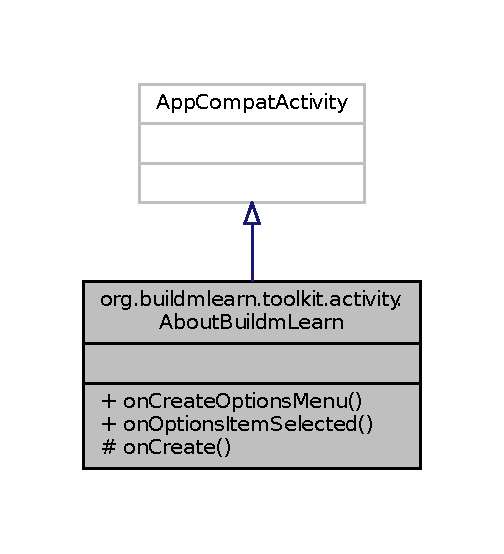
\includegraphics[width=242pt]{d1/dc1/classorg_1_1buildmlearn_1_1toolkit_1_1activity_1_1AboutBuildmLearn__inherit__graph}
\end{center}
\end{figure}


Collaboration diagram for org.\-buildmlearn.\-toolkit.\-activity.\-About\-Buildm\-Learn\-:
\nopagebreak
\begin{figure}[H]
\begin{center}
\leavevmode
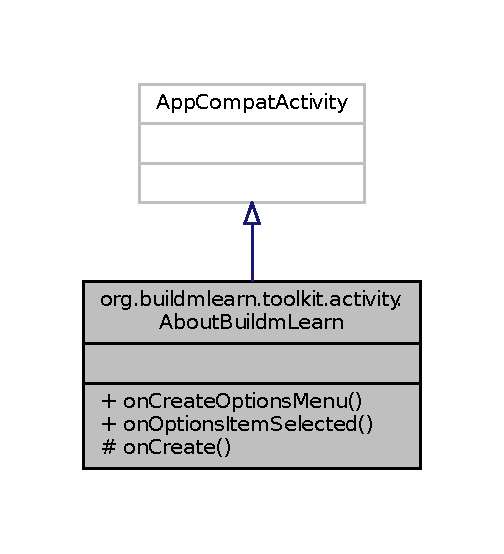
\includegraphics[width=242pt]{da/d3d/classorg_1_1buildmlearn_1_1toolkit_1_1activity_1_1AboutBuildmLearn__coll__graph}
\end{center}
\end{figure}
\subsection*{Public Member Functions}
\begin{DoxyCompactItemize}
\item 
boolean \hyperlink{classorg_1_1buildmlearn_1_1toolkit_1_1activity_1_1AboutBuildmLearn_aae36faad42229bef35356768eb2456ea}{on\-Create\-Options\-Menu} (Menu menu)
\item 
boolean \hyperlink{classorg_1_1buildmlearn_1_1toolkit_1_1activity_1_1AboutBuildmLearn_adb420eeaf2bf93bff38b52f19bc16b31}{on\-Options\-Item\-Selected} (Menu\-Item item)
\end{DoxyCompactItemize}
\subsection*{Protected Member Functions}
\begin{DoxyCompactItemize}
\item 
void \hyperlink{classorg_1_1buildmlearn_1_1toolkit_1_1activity_1_1AboutBuildmLearn_af8c59cecea3366aea895a28331d01e9b}{on\-Create} (Bundle saved\-Instance\-State)
\end{DoxyCompactItemize}


\subsection{Detailed Description}
Gives brief info about Buildm\-Learn community and toolkit. 

\subsection{Member Function Documentation}
\hypertarget{classorg_1_1buildmlearn_1_1toolkit_1_1activity_1_1AboutBuildmLearn_af8c59cecea3366aea895a28331d01e9b}{\index{org\-::buildmlearn\-::toolkit\-::activity\-::\-About\-Buildm\-Learn@{org\-::buildmlearn\-::toolkit\-::activity\-::\-About\-Buildm\-Learn}!on\-Create@{on\-Create}}
\index{on\-Create@{on\-Create}!org::buildmlearn::toolkit::activity::AboutBuildmLearn@{org\-::buildmlearn\-::toolkit\-::activity\-::\-About\-Buildm\-Learn}}
\subsubsection[{on\-Create}]{\setlength{\rightskip}{0pt plus 5cm}void org.\-buildmlearn.\-toolkit.\-activity.\-About\-Buildm\-Learn.\-on\-Create (
\begin{DoxyParamCaption}
\item[{Bundle}]{saved\-Instance\-State}
\end{DoxyParamCaption}
)\hspace{0.3cm}{\ttfamily [protected]}}}\label{classorg_1_1buildmlearn_1_1toolkit_1_1activity_1_1AboutBuildmLearn_af8c59cecea3366aea895a28331d01e9b}

\begin{DoxyCode}
20                                                        \{
21         super.onCreate(savedInstanceState);
22         setContentView(R.layout.activity\_about\_buildm\_learn);
23 
24         setSupportActionBar((Toolbar) findViewById(R.id.toolbar));
25         getSupportActionBar().setDisplayHomeAsUpEnabled(\textcolor{keyword}{true});
26 
27 
28     \}
\end{DoxyCode}
\hypertarget{classorg_1_1buildmlearn_1_1toolkit_1_1activity_1_1AboutBuildmLearn_aae36faad42229bef35356768eb2456ea}{\index{org\-::buildmlearn\-::toolkit\-::activity\-::\-About\-Buildm\-Learn@{org\-::buildmlearn\-::toolkit\-::activity\-::\-About\-Buildm\-Learn}!on\-Create\-Options\-Menu@{on\-Create\-Options\-Menu}}
\index{on\-Create\-Options\-Menu@{on\-Create\-Options\-Menu}!org::buildmlearn::toolkit::activity::AboutBuildmLearn@{org\-::buildmlearn\-::toolkit\-::activity\-::\-About\-Buildm\-Learn}}
\subsubsection[{on\-Create\-Options\-Menu}]{\setlength{\rightskip}{0pt plus 5cm}boolean org.\-buildmlearn.\-toolkit.\-activity.\-About\-Buildm\-Learn.\-on\-Create\-Options\-Menu (
\begin{DoxyParamCaption}
\item[{Menu}]{menu}
\end{DoxyParamCaption}
)}}\label{classorg_1_1buildmlearn_1_1toolkit_1_1activity_1_1AboutBuildmLearn_aae36faad42229bef35356768eb2456ea}

\begin{DoxyCode}
34                                                   \{
35         \textcolor{comment}{// Inflate the menu; this adds items to the action bar if it is present.}
36         getMenuInflater().inflate(R.menu.menu\_about\_buildm\_learn, menu);
37         \textcolor{keywordflow}{return} \textcolor{keyword}{true};
38     \}
\end{DoxyCode}
\hypertarget{classorg_1_1buildmlearn_1_1toolkit_1_1activity_1_1AboutBuildmLearn_adb420eeaf2bf93bff38b52f19bc16b31}{\index{org\-::buildmlearn\-::toolkit\-::activity\-::\-About\-Buildm\-Learn@{org\-::buildmlearn\-::toolkit\-::activity\-::\-About\-Buildm\-Learn}!on\-Options\-Item\-Selected@{on\-Options\-Item\-Selected}}
\index{on\-Options\-Item\-Selected@{on\-Options\-Item\-Selected}!org::buildmlearn::toolkit::activity::AboutBuildmLearn@{org\-::buildmlearn\-::toolkit\-::activity\-::\-About\-Buildm\-Learn}}
\subsubsection[{on\-Options\-Item\-Selected}]{\setlength{\rightskip}{0pt plus 5cm}boolean org.\-buildmlearn.\-toolkit.\-activity.\-About\-Buildm\-Learn.\-on\-Options\-Item\-Selected (
\begin{DoxyParamCaption}
\item[{Menu\-Item}]{item}
\end{DoxyParamCaption}
)}}\label{classorg_1_1buildmlearn_1_1toolkit_1_1activity_1_1AboutBuildmLearn_adb420eeaf2bf93bff38b52f19bc16b31}

\begin{DoxyCode}
44                                                         \{
45         \textcolor{comment}{// Handle action bar item clicks here. The action bar will}
46         \textcolor{comment}{// automatically handle clicks on the Home/Up button, so long}
47         \textcolor{comment}{// as you specify a parent activity in AndroidManifest.xml.}
48         \textcolor{keywordtype}{int} \textcolor{keywordtype}{id} = item.getItemId();
49 
50         \textcolor{comment}{//noinspection SimplifiableIfStatement}
51         \textcolor{keywordflow}{if} (\textcolor{keywordtype}{id} == R.id.action\_settings) \{
52             \textcolor{keywordflow}{return} \textcolor{keyword}{true};
53         \}
54 
55         \textcolor{keywordflow}{return} super.onOptionsItemSelected(item);
56     \}
\end{DoxyCode}


The documentation for this class was generated from the following file\-:\begin{DoxyCompactItemize}
\item 
/\-Buildm\-Learn-\/\-Toolkit-\/\-Android/source-\/code/app/src/main/java/org/buildmlearn/toolkit/activity/\hyperlink{AboutBuildmLearn_8java}{About\-Buildm\-Learn.\-java}\end{DoxyCompactItemize}

\hypertarget{classorg_1_1buildmlearn_1_1toolkit_1_1utilities_1_1Alias}{\section{org.\-buildmlearn.\-toolkit.\-utilities.\-Alias Class Reference}
\label{classorg_1_1buildmlearn_1_1toolkit_1_1utilities_1_1Alias}\index{org.\-buildmlearn.\-toolkit.\-utilities.\-Alias@{org.\-buildmlearn.\-toolkit.\-utilities.\-Alias}}
}


Model class for storing \hyperlink{classorg_1_1buildmlearn_1_1toolkit_1_1utilities_1_1Alias}{Alias} data for keystore.  




Collaboration diagram for org.\-buildmlearn.\-toolkit.\-utilities.\-Alias\-:
\nopagebreak
\begin{figure}[H]
\begin{center}
\leavevmode
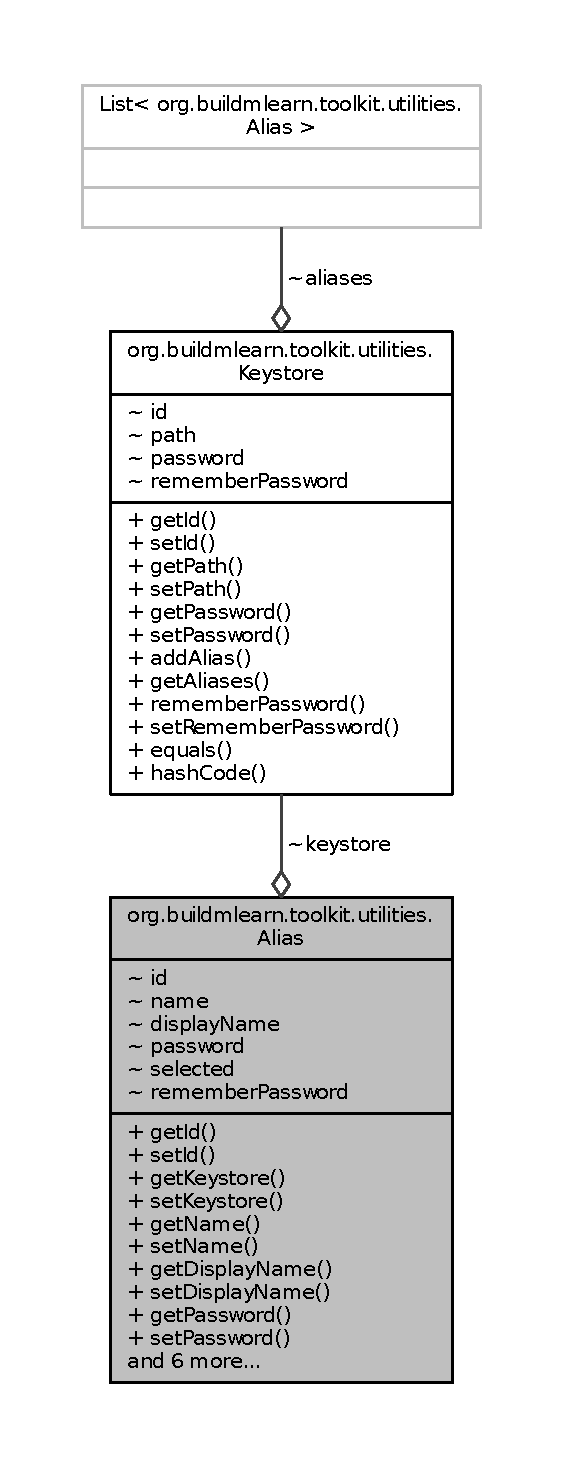
\includegraphics[height=550pt]{d5/dab/classorg_1_1buildmlearn_1_1toolkit_1_1utilities_1_1Alias__coll__graph}
\end{center}
\end{figure}
\subsection*{Public Member Functions}
\begin{DoxyCompactItemize}
\item 
long \hyperlink{classorg_1_1buildmlearn_1_1toolkit_1_1utilities_1_1Alias_ad854360fe849540917362f3fda65b118}{get\-Id} ()
\item 
void \hyperlink{classorg_1_1buildmlearn_1_1toolkit_1_1utilities_1_1Alias_a46050f92ad4ea5360c50aa865c177ff1}{set\-Id} (long id)
\item 
\hyperlink{classorg_1_1buildmlearn_1_1toolkit_1_1utilities_1_1Keystore}{Keystore} \hyperlink{classorg_1_1buildmlearn_1_1toolkit_1_1utilities_1_1Alias_ae6fd9833900335696443e219d50e900e}{get\-Keystore} ()
\item 
void \hyperlink{classorg_1_1buildmlearn_1_1toolkit_1_1utilities_1_1Alias_a1b6a7ec467e6a3a20794086af1f34057}{set\-Keystore} (\hyperlink{classorg_1_1buildmlearn_1_1toolkit_1_1utilities_1_1Keystore}{Keystore} keystore)
\item 
String \hyperlink{classorg_1_1buildmlearn_1_1toolkit_1_1utilities_1_1Alias_a0bb609953ae521ac184a0cf3ed347703}{get\-Name} ()
\item 
void \hyperlink{classorg_1_1buildmlearn_1_1toolkit_1_1utilities_1_1Alias_a78e04df1f7e80d248a219d89c91a6034}{set\-Name} (String name)
\item 
String \hyperlink{classorg_1_1buildmlearn_1_1toolkit_1_1utilities_1_1Alias_adc60c0bcd710831f5a9281c3ef884d0d}{get\-Display\-Name} ()
\item 
void \hyperlink{classorg_1_1buildmlearn_1_1toolkit_1_1utilities_1_1Alias_a3b06eeb819f1640f253022a44fa925cc}{set\-Display\-Name} (String display\-Name)
\item 
String \hyperlink{classorg_1_1buildmlearn_1_1toolkit_1_1utilities_1_1Alias_aa19ddc355d3eac8fa1317b6ebe66fe30}{get\-Password} ()
\item 
void \hyperlink{classorg_1_1buildmlearn_1_1toolkit_1_1utilities_1_1Alias_a00ba075722c71303485f0991413f659b}{set\-Password} (String password)
\item 
boolean \hyperlink{classorg_1_1buildmlearn_1_1toolkit_1_1utilities_1_1Alias_a0b7267664c59b5c2ebd7eaa300270bc6}{is\-Selected} ()
\item 
void \hyperlink{classorg_1_1buildmlearn_1_1toolkit_1_1utilities_1_1Alias_a31f1875c4a77412a7d9207f285aea841}{set\-Selected} (boolean selected)
\item 
boolean \hyperlink{classorg_1_1buildmlearn_1_1toolkit_1_1utilities_1_1Alias_afaf811300872e304bef8328df31ce3cc}{remember\-Password} ()
\item 
void \hyperlink{classorg_1_1buildmlearn_1_1toolkit_1_1utilities_1_1Alias_a761275eebde7f3c1900bc0c627ffc3ae}{set\-Remember\-Password} (boolean remember\-Password)
\item 
boolean \hyperlink{classorg_1_1buildmlearn_1_1toolkit_1_1utilities_1_1Alias_a5a34c06a2fd102242a9a6fa97846ca3d}{equals} (Object o)
\item 
int \hyperlink{classorg_1_1buildmlearn_1_1toolkit_1_1utilities_1_1Alias_a8ca9bfa9fd2e0441decc1ab8169a7e05}{hash\-Code} ()
\end{DoxyCompactItemize}


\subsection{Detailed Description}
Model class for storing \hyperlink{classorg_1_1buildmlearn_1_1toolkit_1_1utilities_1_1Alias}{Alias} data for keystore. 

\subsection{Member Function Documentation}
\hypertarget{classorg_1_1buildmlearn_1_1toolkit_1_1utilities_1_1Alias_a5a34c06a2fd102242a9a6fa97846ca3d}{\index{org\-::buildmlearn\-::toolkit\-::utilities\-::\-Alias@{org\-::buildmlearn\-::toolkit\-::utilities\-::\-Alias}!equals@{equals}}
\index{equals@{equals}!org::buildmlearn::toolkit::utilities::Alias@{org\-::buildmlearn\-::toolkit\-::utilities\-::\-Alias}}
\subsubsection[{equals}]{\setlength{\rightskip}{0pt plus 5cm}boolean org.\-buildmlearn.\-toolkit.\-utilities.\-Alias.\-equals (
\begin{DoxyParamCaption}
\item[{Object}]{o}
\end{DoxyParamCaption}
)}}\label{classorg_1_1buildmlearn_1_1toolkit_1_1utilities_1_1Alias_a5a34c06a2fd102242a9a6fa97846ca3d}

\begin{DoxyCode}
73                                     \{
74         \textcolor{keywordflow}{if} (\textcolor{keyword}{this} == o) \textcolor{keywordflow}{return} \textcolor{keyword}{true};
75         \textcolor{keywordflow}{if} (o == null || getClass() != o.getClass()) \textcolor{keywordflow}{return} \textcolor{keyword}{false};
76 
77         Alias alias = (Alias) o;
78 
79         \textcolor{keywordflow}{if} (\textcolor{keywordtype}{id} != alias.id) \textcolor{keywordflow}{return} \textcolor{keyword}{false};
80 
81         \textcolor{keywordflow}{return} \textcolor{keyword}{true};
82     \}
\end{DoxyCode}
\hypertarget{classorg_1_1buildmlearn_1_1toolkit_1_1utilities_1_1Alias_adc60c0bcd710831f5a9281c3ef884d0d}{\index{org\-::buildmlearn\-::toolkit\-::utilities\-::\-Alias@{org\-::buildmlearn\-::toolkit\-::utilities\-::\-Alias}!get\-Display\-Name@{get\-Display\-Name}}
\index{get\-Display\-Name@{get\-Display\-Name}!org::buildmlearn::toolkit::utilities::Alias@{org\-::buildmlearn\-::toolkit\-::utilities\-::\-Alias}}
\subsubsection[{get\-Display\-Name}]{\setlength{\rightskip}{0pt plus 5cm}String org.\-buildmlearn.\-toolkit.\-utilities.\-Alias.\-get\-Display\-Name (
\begin{DoxyParamCaption}
{}
\end{DoxyParamCaption}
)}}\label{classorg_1_1buildmlearn_1_1toolkit_1_1utilities_1_1Alias_adc60c0bcd710831f5a9281c3ef884d0d}

\begin{DoxyCode}
40                                    \{
41         \textcolor{keywordflow}{return} displayName;
42     \}
\end{DoxyCode}
\hypertarget{classorg_1_1buildmlearn_1_1toolkit_1_1utilities_1_1Alias_ad854360fe849540917362f3fda65b118}{\index{org\-::buildmlearn\-::toolkit\-::utilities\-::\-Alias@{org\-::buildmlearn\-::toolkit\-::utilities\-::\-Alias}!get\-Id@{get\-Id}}
\index{get\-Id@{get\-Id}!org::buildmlearn::toolkit::utilities::Alias@{org\-::buildmlearn\-::toolkit\-::utilities\-::\-Alias}}
\subsubsection[{get\-Id}]{\setlength{\rightskip}{0pt plus 5cm}long org.\-buildmlearn.\-toolkit.\-utilities.\-Alias.\-get\-Id (
\begin{DoxyParamCaption}
{}
\end{DoxyParamCaption}
)}}\label{classorg_1_1buildmlearn_1_1toolkit_1_1utilities_1_1Alias_ad854360fe849540917362f3fda65b118}

\begin{DoxyCode}
16                         \{
17         \textcolor{keywordflow}{return} id;
18     \}
\end{DoxyCode}
\hypertarget{classorg_1_1buildmlearn_1_1toolkit_1_1utilities_1_1Alias_ae6fd9833900335696443e219d50e900e}{\index{org\-::buildmlearn\-::toolkit\-::utilities\-::\-Alias@{org\-::buildmlearn\-::toolkit\-::utilities\-::\-Alias}!get\-Keystore@{get\-Keystore}}
\index{get\-Keystore@{get\-Keystore}!org::buildmlearn::toolkit::utilities::Alias@{org\-::buildmlearn\-::toolkit\-::utilities\-::\-Alias}}
\subsubsection[{get\-Keystore}]{\setlength{\rightskip}{0pt plus 5cm}{\bf Keystore} org.\-buildmlearn.\-toolkit.\-utilities.\-Alias.\-get\-Keystore (
\begin{DoxyParamCaption}
{}
\end{DoxyParamCaption}
)}}\label{classorg_1_1buildmlearn_1_1toolkit_1_1utilities_1_1Alias_ae6fd9833900335696443e219d50e900e}

\begin{DoxyCode}
24                                   \{
25         \textcolor{keywordflow}{return} keystore;
26     \}
\end{DoxyCode}
\hypertarget{classorg_1_1buildmlearn_1_1toolkit_1_1utilities_1_1Alias_a0bb609953ae521ac184a0cf3ed347703}{\index{org\-::buildmlearn\-::toolkit\-::utilities\-::\-Alias@{org\-::buildmlearn\-::toolkit\-::utilities\-::\-Alias}!get\-Name@{get\-Name}}
\index{get\-Name@{get\-Name}!org::buildmlearn::toolkit::utilities::Alias@{org\-::buildmlearn\-::toolkit\-::utilities\-::\-Alias}}
\subsubsection[{get\-Name}]{\setlength{\rightskip}{0pt plus 5cm}String org.\-buildmlearn.\-toolkit.\-utilities.\-Alias.\-get\-Name (
\begin{DoxyParamCaption}
{}
\end{DoxyParamCaption}
)}}\label{classorg_1_1buildmlearn_1_1toolkit_1_1utilities_1_1Alias_a0bb609953ae521ac184a0cf3ed347703}

\begin{DoxyCode}
32                             \{
33         \textcolor{keywordflow}{return} name;
34     \}
\end{DoxyCode}
\hypertarget{classorg_1_1buildmlearn_1_1toolkit_1_1utilities_1_1Alias_aa19ddc355d3eac8fa1317b6ebe66fe30}{\index{org\-::buildmlearn\-::toolkit\-::utilities\-::\-Alias@{org\-::buildmlearn\-::toolkit\-::utilities\-::\-Alias}!get\-Password@{get\-Password}}
\index{get\-Password@{get\-Password}!org::buildmlearn::toolkit::utilities::Alias@{org\-::buildmlearn\-::toolkit\-::utilities\-::\-Alias}}
\subsubsection[{get\-Password}]{\setlength{\rightskip}{0pt plus 5cm}String org.\-buildmlearn.\-toolkit.\-utilities.\-Alias.\-get\-Password (
\begin{DoxyParamCaption}
{}
\end{DoxyParamCaption}
)}}\label{classorg_1_1buildmlearn_1_1toolkit_1_1utilities_1_1Alias_aa19ddc355d3eac8fa1317b6ebe66fe30}

\begin{DoxyCode}
48                                 \{
49         \textcolor{keywordflow}{return} password;
50     \}
\end{DoxyCode}
\hypertarget{classorg_1_1buildmlearn_1_1toolkit_1_1utilities_1_1Alias_a8ca9bfa9fd2e0441decc1ab8169a7e05}{\index{org\-::buildmlearn\-::toolkit\-::utilities\-::\-Alias@{org\-::buildmlearn\-::toolkit\-::utilities\-::\-Alias}!hash\-Code@{hash\-Code}}
\index{hash\-Code@{hash\-Code}!org::buildmlearn::toolkit::utilities::Alias@{org\-::buildmlearn\-::toolkit\-::utilities\-::\-Alias}}
\subsubsection[{hash\-Code}]{\setlength{\rightskip}{0pt plus 5cm}int org.\-buildmlearn.\-toolkit.\-utilities.\-Alias.\-hash\-Code (
\begin{DoxyParamCaption}
{}
\end{DoxyParamCaption}
)}}\label{classorg_1_1buildmlearn_1_1toolkit_1_1utilities_1_1Alias_a8ca9bfa9fd2e0441decc1ab8169a7e05}

\begin{DoxyCode}
85                           \{
86         \textcolor{keywordflow}{return} (\textcolor{keywordtype}{int}) (\textcolor{keywordtype}{id} ^ (\textcolor{keywordtype}{id} >>> 32));
87     \}
\end{DoxyCode}
\hypertarget{classorg_1_1buildmlearn_1_1toolkit_1_1utilities_1_1Alias_a0b7267664c59b5c2ebd7eaa300270bc6}{\index{org\-::buildmlearn\-::toolkit\-::utilities\-::\-Alias@{org\-::buildmlearn\-::toolkit\-::utilities\-::\-Alias}!is\-Selected@{is\-Selected}}
\index{is\-Selected@{is\-Selected}!org::buildmlearn::toolkit::utilities::Alias@{org\-::buildmlearn\-::toolkit\-::utilities\-::\-Alias}}
\subsubsection[{is\-Selected}]{\setlength{\rightskip}{0pt plus 5cm}boolean org.\-buildmlearn.\-toolkit.\-utilities.\-Alias.\-is\-Selected (
\begin{DoxyParamCaption}
{}
\end{DoxyParamCaption}
)}}\label{classorg_1_1buildmlearn_1_1toolkit_1_1utilities_1_1Alias_a0b7267664c59b5c2ebd7eaa300270bc6}

\begin{DoxyCode}
56                                 \{
57         \textcolor{keywordflow}{return} selected;
58     \}
\end{DoxyCode}
\hypertarget{classorg_1_1buildmlearn_1_1toolkit_1_1utilities_1_1Alias_afaf811300872e304bef8328df31ce3cc}{\index{org\-::buildmlearn\-::toolkit\-::utilities\-::\-Alias@{org\-::buildmlearn\-::toolkit\-::utilities\-::\-Alias}!remember\-Password@{remember\-Password}}
\index{remember\-Password@{remember\-Password}!org::buildmlearn::toolkit::utilities::Alias@{org\-::buildmlearn\-::toolkit\-::utilities\-::\-Alias}}
\subsubsection[{remember\-Password}]{\setlength{\rightskip}{0pt plus 5cm}boolean org.\-buildmlearn.\-toolkit.\-utilities.\-Alias.\-remember\-Password (
\begin{DoxyParamCaption}
{}
\end{DoxyParamCaption}
)}}\label{classorg_1_1buildmlearn_1_1toolkit_1_1utilities_1_1Alias_afaf811300872e304bef8328df31ce3cc}

\begin{DoxyCode}
64                                       \{
65         \textcolor{keywordflow}{return} \hyperlink{classorg_1_1buildmlearn_1_1toolkit_1_1utilities_1_1Alias_afaf811300872e304bef8328df31ce3cc}{rememberPassword};
66     \}
\end{DoxyCode}
\hypertarget{classorg_1_1buildmlearn_1_1toolkit_1_1utilities_1_1Alias_a3b06eeb819f1640f253022a44fa925cc}{\index{org\-::buildmlearn\-::toolkit\-::utilities\-::\-Alias@{org\-::buildmlearn\-::toolkit\-::utilities\-::\-Alias}!set\-Display\-Name@{set\-Display\-Name}}
\index{set\-Display\-Name@{set\-Display\-Name}!org::buildmlearn::toolkit::utilities::Alias@{org\-::buildmlearn\-::toolkit\-::utilities\-::\-Alias}}
\subsubsection[{set\-Display\-Name}]{\setlength{\rightskip}{0pt plus 5cm}void org.\-buildmlearn.\-toolkit.\-utilities.\-Alias.\-set\-Display\-Name (
\begin{DoxyParamCaption}
\item[{String}]{display\-Name}
\end{DoxyParamCaption}
)}}\label{classorg_1_1buildmlearn_1_1toolkit_1_1utilities_1_1Alias_a3b06eeb819f1640f253022a44fa925cc}

\begin{DoxyCode}
44                                                    \{
45         this.displayName = displayName;
46     \}
\end{DoxyCode}
\hypertarget{classorg_1_1buildmlearn_1_1toolkit_1_1utilities_1_1Alias_a46050f92ad4ea5360c50aa865c177ff1}{\index{org\-::buildmlearn\-::toolkit\-::utilities\-::\-Alias@{org\-::buildmlearn\-::toolkit\-::utilities\-::\-Alias}!set\-Id@{set\-Id}}
\index{set\-Id@{set\-Id}!org::buildmlearn::toolkit::utilities::Alias@{org\-::buildmlearn\-::toolkit\-::utilities\-::\-Alias}}
\subsubsection[{set\-Id}]{\setlength{\rightskip}{0pt plus 5cm}void org.\-buildmlearn.\-toolkit.\-utilities.\-Alias.\-set\-Id (
\begin{DoxyParamCaption}
\item[{long}]{id}
\end{DoxyParamCaption}
)}}\label{classorg_1_1buildmlearn_1_1toolkit_1_1utilities_1_1Alias_a46050f92ad4ea5360c50aa865c177ff1}

\begin{DoxyCode}
20                                \{
21         this.id = id;
22     \}
\end{DoxyCode}
\hypertarget{classorg_1_1buildmlearn_1_1toolkit_1_1utilities_1_1Alias_a1b6a7ec467e6a3a20794086af1f34057}{\index{org\-::buildmlearn\-::toolkit\-::utilities\-::\-Alias@{org\-::buildmlearn\-::toolkit\-::utilities\-::\-Alias}!set\-Keystore@{set\-Keystore}}
\index{set\-Keystore@{set\-Keystore}!org::buildmlearn::toolkit::utilities::Alias@{org\-::buildmlearn\-::toolkit\-::utilities\-::\-Alias}}
\subsubsection[{set\-Keystore}]{\setlength{\rightskip}{0pt plus 5cm}void org.\-buildmlearn.\-toolkit.\-utilities.\-Alias.\-set\-Keystore (
\begin{DoxyParamCaption}
\item[{{\bf Keystore}}]{keystore}
\end{DoxyParamCaption}
)}}\label{classorg_1_1buildmlearn_1_1toolkit_1_1utilities_1_1Alias_a1b6a7ec467e6a3a20794086af1f34057}

\begin{DoxyCode}
28                                                \{
29         this.keystore = keystore;
30     \}
\end{DoxyCode}
\hypertarget{classorg_1_1buildmlearn_1_1toolkit_1_1utilities_1_1Alias_a78e04df1f7e80d248a219d89c91a6034}{\index{org\-::buildmlearn\-::toolkit\-::utilities\-::\-Alias@{org\-::buildmlearn\-::toolkit\-::utilities\-::\-Alias}!set\-Name@{set\-Name}}
\index{set\-Name@{set\-Name}!org::buildmlearn::toolkit::utilities::Alias@{org\-::buildmlearn\-::toolkit\-::utilities\-::\-Alias}}
\subsubsection[{set\-Name}]{\setlength{\rightskip}{0pt plus 5cm}void org.\-buildmlearn.\-toolkit.\-utilities.\-Alias.\-set\-Name (
\begin{DoxyParamCaption}
\item[{String}]{name}
\end{DoxyParamCaption}
)}}\label{classorg_1_1buildmlearn_1_1toolkit_1_1utilities_1_1Alias_a78e04df1f7e80d248a219d89c91a6034}

\begin{DoxyCode}
36                                      \{
37         this.name = name;
38     \}
\end{DoxyCode}
\hypertarget{classorg_1_1buildmlearn_1_1toolkit_1_1utilities_1_1Alias_a00ba075722c71303485f0991413f659b}{\index{org\-::buildmlearn\-::toolkit\-::utilities\-::\-Alias@{org\-::buildmlearn\-::toolkit\-::utilities\-::\-Alias}!set\-Password@{set\-Password}}
\index{set\-Password@{set\-Password}!org::buildmlearn::toolkit::utilities::Alias@{org\-::buildmlearn\-::toolkit\-::utilities\-::\-Alias}}
\subsubsection[{set\-Password}]{\setlength{\rightskip}{0pt plus 5cm}void org.\-buildmlearn.\-toolkit.\-utilities.\-Alias.\-set\-Password (
\begin{DoxyParamCaption}
\item[{String}]{password}
\end{DoxyParamCaption}
)}}\label{classorg_1_1buildmlearn_1_1toolkit_1_1utilities_1_1Alias_a00ba075722c71303485f0991413f659b}

\begin{DoxyCode}
52                                              \{
53         this.password = password;
54     \}
\end{DoxyCode}
\hypertarget{classorg_1_1buildmlearn_1_1toolkit_1_1utilities_1_1Alias_a761275eebde7f3c1900bc0c627ffc3ae}{\index{org\-::buildmlearn\-::toolkit\-::utilities\-::\-Alias@{org\-::buildmlearn\-::toolkit\-::utilities\-::\-Alias}!set\-Remember\-Password@{set\-Remember\-Password}}
\index{set\-Remember\-Password@{set\-Remember\-Password}!org::buildmlearn::toolkit::utilities::Alias@{org\-::buildmlearn\-::toolkit\-::utilities\-::\-Alias}}
\subsubsection[{set\-Remember\-Password}]{\setlength{\rightskip}{0pt plus 5cm}void org.\-buildmlearn.\-toolkit.\-utilities.\-Alias.\-set\-Remember\-Password (
\begin{DoxyParamCaption}
\item[{boolean}]{remember\-Password}
\end{DoxyParamCaption}
)}}\label{classorg_1_1buildmlearn_1_1toolkit_1_1utilities_1_1Alias_a761275eebde7f3c1900bc0c627ffc3ae}

\begin{DoxyCode}
68                                                               \{
69         this.rememberPassword = \hyperlink{classorg_1_1buildmlearn_1_1toolkit_1_1utilities_1_1Alias_afaf811300872e304bef8328df31ce3cc}{rememberPassword};
70     \}
\end{DoxyCode}
\hypertarget{classorg_1_1buildmlearn_1_1toolkit_1_1utilities_1_1Alias_a31f1875c4a77412a7d9207f285aea841}{\index{org\-::buildmlearn\-::toolkit\-::utilities\-::\-Alias@{org\-::buildmlearn\-::toolkit\-::utilities\-::\-Alias}!set\-Selected@{set\-Selected}}
\index{set\-Selected@{set\-Selected}!org::buildmlearn::toolkit::utilities::Alias@{org\-::buildmlearn\-::toolkit\-::utilities\-::\-Alias}}
\subsubsection[{set\-Selected}]{\setlength{\rightskip}{0pt plus 5cm}void org.\-buildmlearn.\-toolkit.\-utilities.\-Alias.\-set\-Selected (
\begin{DoxyParamCaption}
\item[{boolean}]{selected}
\end{DoxyParamCaption}
)}}\label{classorg_1_1buildmlearn_1_1toolkit_1_1utilities_1_1Alias_a31f1875c4a77412a7d9207f285aea841}

\begin{DoxyCode}
60                                               \{
61         this.selected = selected;
62     \}
\end{DoxyCode}


The documentation for this class was generated from the following file\-:\begin{DoxyCompactItemize}
\item 
/\-Buildm\-Learn-\/\-Toolkit-\/\-Android/source-\/code/app/src/main/java/org/buildmlearn/toolkit/utilities/\hyperlink{Alias_8java}{Alias.\-java}\end{DoxyCompactItemize}

\hypertarget{classorg_1_1buildmlearn_1_1toolkit_1_1constant_1_1Constants}{\section{org.\-buildmlearn.\-toolkit.\-constant.\-Constants Class Reference}
\label{classorg_1_1buildmlearn_1_1toolkit_1_1constant_1_1Constants}\index{org.\-buildmlearn.\-toolkit.\-constant.\-Constants@{org.\-buildmlearn.\-toolkit.\-constant.\-Constants}}
}


\hyperlink{classorg_1_1buildmlearn_1_1toolkit_1_1constant_1_1Constants}{Constants} related project directories, preferences and keys.  




Collaboration diagram for org.\-buildmlearn.\-toolkit.\-constant.\-Constants\-:
\nopagebreak
\begin{figure}[H]
\begin{center}
\leavevmode
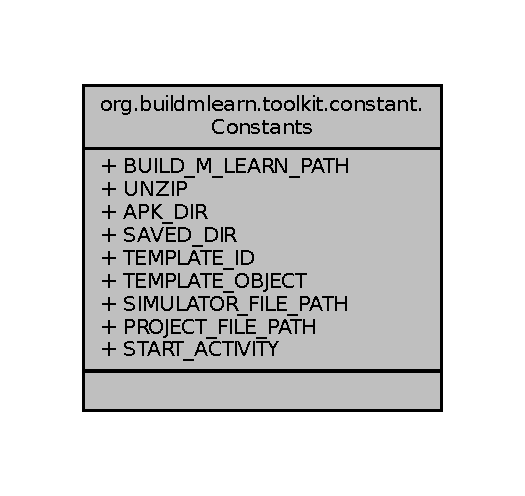
\includegraphics[width=252pt]{d3/d2c/classorg_1_1buildmlearn_1_1toolkit_1_1constant_1_1Constants__coll__graph}
\end{center}
\end{figure}
\subsection*{Static Public Attributes}
\begin{DoxyCompactItemize}
\item 
static final String \hyperlink{classorg_1_1buildmlearn_1_1toolkit_1_1constant_1_1Constants_a9965876f735c5e8a6b5b1b187878da87}{B\-U\-I\-L\-D\-\_\-\-M\-\_\-\-L\-E\-A\-R\-N\-\_\-\-P\-A\-T\-H} = \char`\"{}/Buildm\-Learn/\char`\"{}
\item 
static final String \hyperlink{classorg_1_1buildmlearn_1_1toolkit_1_1constant_1_1Constants_aa7187aa1863aeed8b73d71e3d203fe3c}{U\-N\-Z\-I\-P} = \hyperlink{classorg_1_1buildmlearn_1_1toolkit_1_1constant_1_1Constants_a9965876f735c5e8a6b5b1b187878da87}{B\-U\-I\-L\-D\-\_\-\-M\-\_\-\-L\-E\-A\-R\-N\-\_\-\-P\-A\-T\-H} + \char`\"{}unzipped/\char`\"{}
\item 
static final String \hyperlink{classorg_1_1buildmlearn_1_1toolkit_1_1constant_1_1Constants_ad32e350b2a3bc331971d274727ce69c5}{A\-P\-K\-\_\-\-D\-I\-R} = \hyperlink{classorg_1_1buildmlearn_1_1toolkit_1_1constant_1_1Constants_a9965876f735c5e8a6b5b1b187878da87}{B\-U\-I\-L\-D\-\_\-\-M\-\_\-\-L\-E\-A\-R\-N\-\_\-\-P\-A\-T\-H} + \char`\"{}apk/\char`\"{}
\item 
static final String \hyperlink{classorg_1_1buildmlearn_1_1toolkit_1_1constant_1_1Constants_a657c90b7a9ba3bfd833cead98e2d9841}{S\-A\-V\-E\-D\-\_\-\-D\-I\-R} = \hyperlink{classorg_1_1buildmlearn_1_1toolkit_1_1constant_1_1Constants_a9965876f735c5e8a6b5b1b187878da87}{B\-U\-I\-L\-D\-\_\-\-M\-\_\-\-L\-E\-A\-R\-N\-\_\-\-P\-A\-T\-H} + \char`\"{}saved/\char`\"{}
\item 
static final String \hyperlink{classorg_1_1buildmlearn_1_1toolkit_1_1constant_1_1Constants_a2ee9d59d6a353dc4664ed2e2086dae9d}{T\-E\-M\-P\-L\-A\-T\-E\-\_\-\-I\-D} = \char`\"{}T\-E\-M\-P\-L\-A\-T\-E\-\_\-\-I\-D\char`\"{}
\item 
static final String \hyperlink{classorg_1_1buildmlearn_1_1toolkit_1_1constant_1_1Constants_a9e2658a69f3f70584955bbdc947ca0bc}{T\-E\-M\-P\-L\-A\-T\-E\-\_\-\-O\-B\-J\-E\-C\-T} = \char`\"{}T\-E\-M\-P\-L\-A\-T\-E\-\_\-\-O\-B\-J\-E\-C\-T\char`\"{}
\item 
static final String \hyperlink{classorg_1_1buildmlearn_1_1toolkit_1_1constant_1_1Constants_a5e8ea6ec23e727cbfc84e5b854ae311c}{S\-I\-M\-U\-L\-A\-T\-O\-R\-\_\-\-F\-I\-L\-E\-\_\-\-P\-A\-T\-H} = \char`\"{}S\-I\-M\-U\-L\-A\-T\-O\-R\-\_\-\-F\-I\-L\-E\-\_\-\-P\-A\-T\-H\char`\"{}
\item 
static final String \hyperlink{classorg_1_1buildmlearn_1_1toolkit_1_1constant_1_1Constants_ab2586e8aa144cd7e8b4928186d709ea8}{P\-R\-O\-J\-E\-C\-T\-\_\-\-F\-I\-L\-E\-\_\-\-P\-A\-T\-H} = \char`\"{}P\-R\-O\-J\-E\-C\-T\-\_\-\-F\-I\-L\-E\-\_\-\-P\-A\-T\-H\char`\"{}
\item 
static final String \hyperlink{classorg_1_1buildmlearn_1_1toolkit_1_1constant_1_1Constants_a2799e097282009a747db0225f72508ff}{S\-T\-A\-R\-T\-\_\-\-A\-C\-T\-I\-V\-I\-T\-Y} = \char`\"{}S\-T\-A\-R\-T\-\_\-\-A\-C\-T\-I\-V\-I\-T\-Y\char`\"{}
\end{DoxyCompactItemize}


\subsection{Detailed Description}
\hyperlink{classorg_1_1buildmlearn_1_1toolkit_1_1constant_1_1Constants}{Constants} related project directories, preferences and keys. 

Created by Abhishek on 21/04/15. 

\subsection{Member Data Documentation}
\hypertarget{classorg_1_1buildmlearn_1_1toolkit_1_1constant_1_1Constants_ad32e350b2a3bc331971d274727ce69c5}{\index{org\-::buildmlearn\-::toolkit\-::constant\-::\-Constants@{org\-::buildmlearn\-::toolkit\-::constant\-::\-Constants}!A\-P\-K\-\_\-\-D\-I\-R@{A\-P\-K\-\_\-\-D\-I\-R}}
\index{A\-P\-K\-\_\-\-D\-I\-R@{A\-P\-K\-\_\-\-D\-I\-R}!org::buildmlearn::toolkit::constant::Constants@{org\-::buildmlearn\-::toolkit\-::constant\-::\-Constants}}
\subsubsection[{A\-P\-K\-\_\-\-D\-I\-R}]{\setlength{\rightskip}{0pt plus 5cm}final String org.\-buildmlearn.\-toolkit.\-constant.\-Constants.\-A\-P\-K\-\_\-\-D\-I\-R = {\bf B\-U\-I\-L\-D\-\_\-\-M\-\_\-\-L\-E\-A\-R\-N\-\_\-\-P\-A\-T\-H} + \char`\"{}apk/\char`\"{}\hspace{0.3cm}{\ttfamily [static]}}}\label{classorg_1_1buildmlearn_1_1toolkit_1_1constant_1_1Constants_ad32e350b2a3bc331971d274727ce69c5}
\hypertarget{classorg_1_1buildmlearn_1_1toolkit_1_1constant_1_1Constants_a9965876f735c5e8a6b5b1b187878da87}{\index{org\-::buildmlearn\-::toolkit\-::constant\-::\-Constants@{org\-::buildmlearn\-::toolkit\-::constant\-::\-Constants}!B\-U\-I\-L\-D\-\_\-\-M\-\_\-\-L\-E\-A\-R\-N\-\_\-\-P\-A\-T\-H@{B\-U\-I\-L\-D\-\_\-\-M\-\_\-\-L\-E\-A\-R\-N\-\_\-\-P\-A\-T\-H}}
\index{B\-U\-I\-L\-D\-\_\-\-M\-\_\-\-L\-E\-A\-R\-N\-\_\-\-P\-A\-T\-H@{B\-U\-I\-L\-D\-\_\-\-M\-\_\-\-L\-E\-A\-R\-N\-\_\-\-P\-A\-T\-H}!org::buildmlearn::toolkit::constant::Constants@{org\-::buildmlearn\-::toolkit\-::constant\-::\-Constants}}
\subsubsection[{B\-U\-I\-L\-D\-\_\-\-M\-\_\-\-L\-E\-A\-R\-N\-\_\-\-P\-A\-T\-H}]{\setlength{\rightskip}{0pt plus 5cm}final String org.\-buildmlearn.\-toolkit.\-constant.\-Constants.\-B\-U\-I\-L\-D\-\_\-\-M\-\_\-\-L\-E\-A\-R\-N\-\_\-\-P\-A\-T\-H = \char`\"{}/Buildm\-Learn/\char`\"{}\hspace{0.3cm}{\ttfamily [static]}}}\label{classorg_1_1buildmlearn_1_1toolkit_1_1constant_1_1Constants_a9965876f735c5e8a6b5b1b187878da87}
\hypertarget{classorg_1_1buildmlearn_1_1toolkit_1_1constant_1_1Constants_ab2586e8aa144cd7e8b4928186d709ea8}{\index{org\-::buildmlearn\-::toolkit\-::constant\-::\-Constants@{org\-::buildmlearn\-::toolkit\-::constant\-::\-Constants}!P\-R\-O\-J\-E\-C\-T\-\_\-\-F\-I\-L\-E\-\_\-\-P\-A\-T\-H@{P\-R\-O\-J\-E\-C\-T\-\_\-\-F\-I\-L\-E\-\_\-\-P\-A\-T\-H}}
\index{P\-R\-O\-J\-E\-C\-T\-\_\-\-F\-I\-L\-E\-\_\-\-P\-A\-T\-H@{P\-R\-O\-J\-E\-C\-T\-\_\-\-F\-I\-L\-E\-\_\-\-P\-A\-T\-H}!org::buildmlearn::toolkit::constant::Constants@{org\-::buildmlearn\-::toolkit\-::constant\-::\-Constants}}
\subsubsection[{P\-R\-O\-J\-E\-C\-T\-\_\-\-F\-I\-L\-E\-\_\-\-P\-A\-T\-H}]{\setlength{\rightskip}{0pt plus 5cm}final String org.\-buildmlearn.\-toolkit.\-constant.\-Constants.\-P\-R\-O\-J\-E\-C\-T\-\_\-\-F\-I\-L\-E\-\_\-\-P\-A\-T\-H = \char`\"{}P\-R\-O\-J\-E\-C\-T\-\_\-\-F\-I\-L\-E\-\_\-\-P\-A\-T\-H\char`\"{}\hspace{0.3cm}{\ttfamily [static]}}}\label{classorg_1_1buildmlearn_1_1toolkit_1_1constant_1_1Constants_ab2586e8aa144cd7e8b4928186d709ea8}
\hypertarget{classorg_1_1buildmlearn_1_1toolkit_1_1constant_1_1Constants_a657c90b7a9ba3bfd833cead98e2d9841}{\index{org\-::buildmlearn\-::toolkit\-::constant\-::\-Constants@{org\-::buildmlearn\-::toolkit\-::constant\-::\-Constants}!S\-A\-V\-E\-D\-\_\-\-D\-I\-R@{S\-A\-V\-E\-D\-\_\-\-D\-I\-R}}
\index{S\-A\-V\-E\-D\-\_\-\-D\-I\-R@{S\-A\-V\-E\-D\-\_\-\-D\-I\-R}!org::buildmlearn::toolkit::constant::Constants@{org\-::buildmlearn\-::toolkit\-::constant\-::\-Constants}}
\subsubsection[{S\-A\-V\-E\-D\-\_\-\-D\-I\-R}]{\setlength{\rightskip}{0pt plus 5cm}final String org.\-buildmlearn.\-toolkit.\-constant.\-Constants.\-S\-A\-V\-E\-D\-\_\-\-D\-I\-R = {\bf B\-U\-I\-L\-D\-\_\-\-M\-\_\-\-L\-E\-A\-R\-N\-\_\-\-P\-A\-T\-H} + \char`\"{}saved/\char`\"{}\hspace{0.3cm}{\ttfamily [static]}}}\label{classorg_1_1buildmlearn_1_1toolkit_1_1constant_1_1Constants_a657c90b7a9ba3bfd833cead98e2d9841}
\hypertarget{classorg_1_1buildmlearn_1_1toolkit_1_1constant_1_1Constants_a5e8ea6ec23e727cbfc84e5b854ae311c}{\index{org\-::buildmlearn\-::toolkit\-::constant\-::\-Constants@{org\-::buildmlearn\-::toolkit\-::constant\-::\-Constants}!S\-I\-M\-U\-L\-A\-T\-O\-R\-\_\-\-F\-I\-L\-E\-\_\-\-P\-A\-T\-H@{S\-I\-M\-U\-L\-A\-T\-O\-R\-\_\-\-F\-I\-L\-E\-\_\-\-P\-A\-T\-H}}
\index{S\-I\-M\-U\-L\-A\-T\-O\-R\-\_\-\-F\-I\-L\-E\-\_\-\-P\-A\-T\-H@{S\-I\-M\-U\-L\-A\-T\-O\-R\-\_\-\-F\-I\-L\-E\-\_\-\-P\-A\-T\-H}!org::buildmlearn::toolkit::constant::Constants@{org\-::buildmlearn\-::toolkit\-::constant\-::\-Constants}}
\subsubsection[{S\-I\-M\-U\-L\-A\-T\-O\-R\-\_\-\-F\-I\-L\-E\-\_\-\-P\-A\-T\-H}]{\setlength{\rightskip}{0pt plus 5cm}final String org.\-buildmlearn.\-toolkit.\-constant.\-Constants.\-S\-I\-M\-U\-L\-A\-T\-O\-R\-\_\-\-F\-I\-L\-E\-\_\-\-P\-A\-T\-H = \char`\"{}S\-I\-M\-U\-L\-A\-T\-O\-R\-\_\-\-F\-I\-L\-E\-\_\-\-P\-A\-T\-H\char`\"{}\hspace{0.3cm}{\ttfamily [static]}}}\label{classorg_1_1buildmlearn_1_1toolkit_1_1constant_1_1Constants_a5e8ea6ec23e727cbfc84e5b854ae311c}
\hypertarget{classorg_1_1buildmlearn_1_1toolkit_1_1constant_1_1Constants_a2799e097282009a747db0225f72508ff}{\index{org\-::buildmlearn\-::toolkit\-::constant\-::\-Constants@{org\-::buildmlearn\-::toolkit\-::constant\-::\-Constants}!S\-T\-A\-R\-T\-\_\-\-A\-C\-T\-I\-V\-I\-T\-Y@{S\-T\-A\-R\-T\-\_\-\-A\-C\-T\-I\-V\-I\-T\-Y}}
\index{S\-T\-A\-R\-T\-\_\-\-A\-C\-T\-I\-V\-I\-T\-Y@{S\-T\-A\-R\-T\-\_\-\-A\-C\-T\-I\-V\-I\-T\-Y}!org::buildmlearn::toolkit::constant::Constants@{org\-::buildmlearn\-::toolkit\-::constant\-::\-Constants}}
\subsubsection[{S\-T\-A\-R\-T\-\_\-\-A\-C\-T\-I\-V\-I\-T\-Y}]{\setlength{\rightskip}{0pt plus 5cm}final String org.\-buildmlearn.\-toolkit.\-constant.\-Constants.\-S\-T\-A\-R\-T\-\_\-\-A\-C\-T\-I\-V\-I\-T\-Y = \char`\"{}S\-T\-A\-R\-T\-\_\-\-A\-C\-T\-I\-V\-I\-T\-Y\char`\"{}\hspace{0.3cm}{\ttfamily [static]}}}\label{classorg_1_1buildmlearn_1_1toolkit_1_1constant_1_1Constants_a2799e097282009a747db0225f72508ff}
\hypertarget{classorg_1_1buildmlearn_1_1toolkit_1_1constant_1_1Constants_a2ee9d59d6a353dc4664ed2e2086dae9d}{\index{org\-::buildmlearn\-::toolkit\-::constant\-::\-Constants@{org\-::buildmlearn\-::toolkit\-::constant\-::\-Constants}!T\-E\-M\-P\-L\-A\-T\-E\-\_\-\-I\-D@{T\-E\-M\-P\-L\-A\-T\-E\-\_\-\-I\-D}}
\index{T\-E\-M\-P\-L\-A\-T\-E\-\_\-\-I\-D@{T\-E\-M\-P\-L\-A\-T\-E\-\_\-\-I\-D}!org::buildmlearn::toolkit::constant::Constants@{org\-::buildmlearn\-::toolkit\-::constant\-::\-Constants}}
\subsubsection[{T\-E\-M\-P\-L\-A\-T\-E\-\_\-\-I\-D}]{\setlength{\rightskip}{0pt plus 5cm}final String org.\-buildmlearn.\-toolkit.\-constant.\-Constants.\-T\-E\-M\-P\-L\-A\-T\-E\-\_\-\-I\-D = \char`\"{}T\-E\-M\-P\-L\-A\-T\-E\-\_\-\-I\-D\char`\"{}\hspace{0.3cm}{\ttfamily [static]}}}\label{classorg_1_1buildmlearn_1_1toolkit_1_1constant_1_1Constants_a2ee9d59d6a353dc4664ed2e2086dae9d}
\hypertarget{classorg_1_1buildmlearn_1_1toolkit_1_1constant_1_1Constants_a9e2658a69f3f70584955bbdc947ca0bc}{\index{org\-::buildmlearn\-::toolkit\-::constant\-::\-Constants@{org\-::buildmlearn\-::toolkit\-::constant\-::\-Constants}!T\-E\-M\-P\-L\-A\-T\-E\-\_\-\-O\-B\-J\-E\-C\-T@{T\-E\-M\-P\-L\-A\-T\-E\-\_\-\-O\-B\-J\-E\-C\-T}}
\index{T\-E\-M\-P\-L\-A\-T\-E\-\_\-\-O\-B\-J\-E\-C\-T@{T\-E\-M\-P\-L\-A\-T\-E\-\_\-\-O\-B\-J\-E\-C\-T}!org::buildmlearn::toolkit::constant::Constants@{org\-::buildmlearn\-::toolkit\-::constant\-::\-Constants}}
\subsubsection[{T\-E\-M\-P\-L\-A\-T\-E\-\_\-\-O\-B\-J\-E\-C\-T}]{\setlength{\rightskip}{0pt plus 5cm}final String org.\-buildmlearn.\-toolkit.\-constant.\-Constants.\-T\-E\-M\-P\-L\-A\-T\-E\-\_\-\-O\-B\-J\-E\-C\-T = \char`\"{}T\-E\-M\-P\-L\-A\-T\-E\-\_\-\-O\-B\-J\-E\-C\-T\char`\"{}\hspace{0.3cm}{\ttfamily [static]}}}\label{classorg_1_1buildmlearn_1_1toolkit_1_1constant_1_1Constants_a9e2658a69f3f70584955bbdc947ca0bc}
\hypertarget{classorg_1_1buildmlearn_1_1toolkit_1_1constant_1_1Constants_aa7187aa1863aeed8b73d71e3d203fe3c}{\index{org\-::buildmlearn\-::toolkit\-::constant\-::\-Constants@{org\-::buildmlearn\-::toolkit\-::constant\-::\-Constants}!U\-N\-Z\-I\-P@{U\-N\-Z\-I\-P}}
\index{U\-N\-Z\-I\-P@{U\-N\-Z\-I\-P}!org::buildmlearn::toolkit::constant::Constants@{org\-::buildmlearn\-::toolkit\-::constant\-::\-Constants}}
\subsubsection[{U\-N\-Z\-I\-P}]{\setlength{\rightskip}{0pt plus 5cm}final String org.\-buildmlearn.\-toolkit.\-constant.\-Constants.\-U\-N\-Z\-I\-P = {\bf B\-U\-I\-L\-D\-\_\-\-M\-\_\-\-L\-E\-A\-R\-N\-\_\-\-P\-A\-T\-H} + \char`\"{}unzipped/\char`\"{}\hspace{0.3cm}{\ttfamily [static]}}}\label{classorg_1_1buildmlearn_1_1toolkit_1_1constant_1_1Constants_aa7187aa1863aeed8b73d71e3d203fe3c}


The documentation for this class was generated from the following file\-:\begin{DoxyCompactItemize}
\item 
/\-Buildm\-Learn-\/\-Toolkit-\/\-Android/source-\/code/app/src/main/java/org/buildmlearn/toolkit/constant/\hyperlink{Constants_8java}{Constants.\-java}\end{DoxyCompactItemize}

\hypertarget{classorg_1_1buildmlearn_1_1toolkit_1_1learnspelling_1_1DataManager}{\section{org.\-buildmlearn.\-toolkit.\-learnspelling.\-Data\-Manager Class Reference}
\label{classorg_1_1buildmlearn_1_1toolkit_1_1learnspelling_1_1DataManager}\index{org.\-buildmlearn.\-toolkit.\-learnspelling.\-Data\-Manager@{org.\-buildmlearn.\-toolkit.\-learnspelling.\-Data\-Manager}}
}


Simulator code for Learn Spelling Template.  




Collaboration diagram for org.\-buildmlearn.\-toolkit.\-learnspelling.\-Data\-Manager\-:
\nopagebreak
\begin{figure}[H]
\begin{center}
\leavevmode
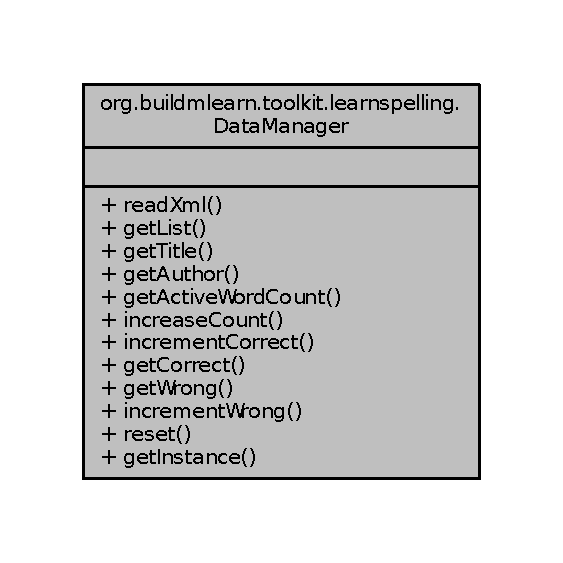
\includegraphics[width=270pt]{dc/d77/classorg_1_1buildmlearn_1_1toolkit_1_1learnspelling_1_1DataManager__coll__graph}
\end{center}
\end{figure}
\subsection*{Public Member Functions}
\begin{DoxyCompactItemize}
\item 
void \hyperlink{classorg_1_1buildmlearn_1_1toolkit_1_1learnspelling_1_1DataManager_a3fd8a313e9ef9dab76725009a3697e0c}{read\-Xml} (String file\-Path)
\item 
Array\-List$<$ \hyperlink{classorg_1_1buildmlearn_1_1toolkit_1_1learnspelling_1_1WordModel}{Word\-Model} $>$ \hyperlink{classorg_1_1buildmlearn_1_1toolkit_1_1learnspelling_1_1DataManager_ae9636c402574a2deaaf3ef9b8a7a14a4}{get\-List} ()
\item 
String \hyperlink{classorg_1_1buildmlearn_1_1toolkit_1_1learnspelling_1_1DataManager_a8b1872c45bc78135989aa0ee7af83f73}{get\-Title} ()
\item 
String \hyperlink{classorg_1_1buildmlearn_1_1toolkit_1_1learnspelling_1_1DataManager_a7cc32c4c6be5e5d70045d0b10f1a2850}{get\-Author} ()
\item 
int \hyperlink{classorg_1_1buildmlearn_1_1toolkit_1_1learnspelling_1_1DataManager_a42a06c0c3ebd9ce4e90d7db5efda93b0}{get\-Active\-Word\-Count} ()
\item 
void \hyperlink{classorg_1_1buildmlearn_1_1toolkit_1_1learnspelling_1_1DataManager_acb93ba29d288da3139c448491c2cb545}{increase\-Count} ()
\item 
void \hyperlink{classorg_1_1buildmlearn_1_1toolkit_1_1learnspelling_1_1DataManager_a4d9d8bdfb3013ee7f60999cccb4c0708}{increment\-Correct} ()
\item 
int \hyperlink{classorg_1_1buildmlearn_1_1toolkit_1_1learnspelling_1_1DataManager_a5544f492cfdf9c117412ac232b390918}{get\-Correct} ()
\item 
int \hyperlink{classorg_1_1buildmlearn_1_1toolkit_1_1learnspelling_1_1DataManager_a18a0de85ba35ec8044f6240ec9f53c7f}{get\-Wrong} ()
\item 
void \hyperlink{classorg_1_1buildmlearn_1_1toolkit_1_1learnspelling_1_1DataManager_a46669a045691413b410a20149180d0a9}{increment\-Wrong} ()
\item 
void \hyperlink{classorg_1_1buildmlearn_1_1toolkit_1_1learnspelling_1_1DataManager_a563486fa47d940f3ce806b8e60f26a8e}{reset} ()
\end{DoxyCompactItemize}
\subsection*{Static Public Member Functions}
\begin{DoxyCompactItemize}
\item 
static \hyperlink{classorg_1_1buildmlearn_1_1toolkit_1_1learnspelling_1_1DataManager}{Data\-Manager} \hyperlink{classorg_1_1buildmlearn_1_1toolkit_1_1learnspelling_1_1DataManager_a7f2efbad139020fb8ec287c16b5b8ea2}{get\-Instance} ()
\end{DoxyCompactItemize}


\subsection{Detailed Description}
Simulator code for Learn Spelling Template. 

\subsection{Member Function Documentation}
\hypertarget{classorg_1_1buildmlearn_1_1toolkit_1_1learnspelling_1_1DataManager_a42a06c0c3ebd9ce4e90d7db5efda93b0}{\index{org\-::buildmlearn\-::toolkit\-::learnspelling\-::\-Data\-Manager@{org\-::buildmlearn\-::toolkit\-::learnspelling\-::\-Data\-Manager}!get\-Active\-Word\-Count@{get\-Active\-Word\-Count}}
\index{get\-Active\-Word\-Count@{get\-Active\-Word\-Count}!org::buildmlearn::toolkit::learnspelling::DataManager@{org\-::buildmlearn\-::toolkit\-::learnspelling\-::\-Data\-Manager}}
\subsubsection[{get\-Active\-Word\-Count}]{\setlength{\rightskip}{0pt plus 5cm}int org.\-buildmlearn.\-toolkit.\-learnspelling.\-Data\-Manager.\-get\-Active\-Word\-Count (
\begin{DoxyParamCaption}
{}
\end{DoxyParamCaption}
)}}\label{classorg_1_1buildmlearn_1_1toolkit_1_1learnspelling_1_1DataManager_a42a06c0c3ebd9ce4e90d7db5efda93b0}

\begin{DoxyCode}
138                                     \{
139         \textcolor{keywordflow}{return} countIndex;
140 
141     \}
\end{DoxyCode}
\hypertarget{classorg_1_1buildmlearn_1_1toolkit_1_1learnspelling_1_1DataManager_a7cc32c4c6be5e5d70045d0b10f1a2850}{\index{org\-::buildmlearn\-::toolkit\-::learnspelling\-::\-Data\-Manager@{org\-::buildmlearn\-::toolkit\-::learnspelling\-::\-Data\-Manager}!get\-Author@{get\-Author}}
\index{get\-Author@{get\-Author}!org::buildmlearn::toolkit::learnspelling::DataManager@{org\-::buildmlearn\-::toolkit\-::learnspelling\-::\-Data\-Manager}}
\subsubsection[{get\-Author}]{\setlength{\rightskip}{0pt plus 5cm}String org.\-buildmlearn.\-toolkit.\-learnspelling.\-Data\-Manager.\-get\-Author (
\begin{DoxyParamCaption}
{}
\end{DoxyParamCaption}
)}}\label{classorg_1_1buildmlearn_1_1toolkit_1_1learnspelling_1_1DataManager_a7cc32c4c6be5e5d70045d0b10f1a2850}

\begin{DoxyCode}
134                               \{
135         \textcolor{keywordflow}{return} mAuthor;
136     \}
\end{DoxyCode}
\hypertarget{classorg_1_1buildmlearn_1_1toolkit_1_1learnspelling_1_1DataManager_a5544f492cfdf9c117412ac232b390918}{\index{org\-::buildmlearn\-::toolkit\-::learnspelling\-::\-Data\-Manager@{org\-::buildmlearn\-::toolkit\-::learnspelling\-::\-Data\-Manager}!get\-Correct@{get\-Correct}}
\index{get\-Correct@{get\-Correct}!org::buildmlearn::toolkit::learnspelling::DataManager@{org\-::buildmlearn\-::toolkit\-::learnspelling\-::\-Data\-Manager}}
\subsubsection[{get\-Correct}]{\setlength{\rightskip}{0pt plus 5cm}int org.\-buildmlearn.\-toolkit.\-learnspelling.\-Data\-Manager.\-get\-Correct (
\begin{DoxyParamCaption}
{}
\end{DoxyParamCaption}
)}}\label{classorg_1_1buildmlearn_1_1toolkit_1_1learnspelling_1_1DataManager_a5544f492cfdf9c117412ac232b390918}

\begin{DoxyCode}
151                             \{
152         \textcolor{keywordflow}{return} countCorrect;
153     \}
\end{DoxyCode}
\hypertarget{classorg_1_1buildmlearn_1_1toolkit_1_1learnspelling_1_1DataManager_a7f2efbad139020fb8ec287c16b5b8ea2}{\index{org\-::buildmlearn\-::toolkit\-::learnspelling\-::\-Data\-Manager@{org\-::buildmlearn\-::toolkit\-::learnspelling\-::\-Data\-Manager}!get\-Instance@{get\-Instance}}
\index{get\-Instance@{get\-Instance}!org::buildmlearn::toolkit::learnspelling::DataManager@{org\-::buildmlearn\-::toolkit\-::learnspelling\-::\-Data\-Manager}}
\subsubsection[{get\-Instance}]{\setlength{\rightskip}{0pt plus 5cm}static {\bf Data\-Manager} org.\-buildmlearn.\-toolkit.\-learnspelling.\-Data\-Manager.\-get\-Instance (
\begin{DoxyParamCaption}
{}
\end{DoxyParamCaption}
)\hspace{0.3cm}{\ttfamily [static]}}}\label{classorg_1_1buildmlearn_1_1toolkit_1_1learnspelling_1_1DataManager_a7f2efbad139020fb8ec287c16b5b8ea2}

\begin{DoxyCode}
62                                             \{
63         \textcolor{keywordflow}{if} (instance == null) \{
64             instance = \textcolor{keyword}{new} DataManager();
65         \}
66         \textcolor{keywordflow}{return} instance;
67     \}
\end{DoxyCode}
\hypertarget{classorg_1_1buildmlearn_1_1toolkit_1_1learnspelling_1_1DataManager_ae9636c402574a2deaaf3ef9b8a7a14a4}{\index{org\-::buildmlearn\-::toolkit\-::learnspelling\-::\-Data\-Manager@{org\-::buildmlearn\-::toolkit\-::learnspelling\-::\-Data\-Manager}!get\-List@{get\-List}}
\index{get\-List@{get\-List}!org::buildmlearn::toolkit::learnspelling::DataManager@{org\-::buildmlearn\-::toolkit\-::learnspelling\-::\-Data\-Manager}}
\subsubsection[{get\-List}]{\setlength{\rightskip}{0pt plus 5cm}Array\-List$<${\bf Word\-Model}$>$ org.\-buildmlearn.\-toolkit.\-learnspelling.\-Data\-Manager.\-get\-List (
\begin{DoxyParamCaption}
{}
\end{DoxyParamCaption}
)}}\label{classorg_1_1buildmlearn_1_1toolkit_1_1learnspelling_1_1DataManager_ae9636c402574a2deaaf3ef9b8a7a14a4}

\begin{DoxyCode}
125                                           \{
126 
127         \textcolor{keywordflow}{return} mList;
128     \}
\end{DoxyCode}
\hypertarget{classorg_1_1buildmlearn_1_1toolkit_1_1learnspelling_1_1DataManager_a8b1872c45bc78135989aa0ee7af83f73}{\index{org\-::buildmlearn\-::toolkit\-::learnspelling\-::\-Data\-Manager@{org\-::buildmlearn\-::toolkit\-::learnspelling\-::\-Data\-Manager}!get\-Title@{get\-Title}}
\index{get\-Title@{get\-Title}!org::buildmlearn::toolkit::learnspelling::DataManager@{org\-::buildmlearn\-::toolkit\-::learnspelling\-::\-Data\-Manager}}
\subsubsection[{get\-Title}]{\setlength{\rightskip}{0pt plus 5cm}String org.\-buildmlearn.\-toolkit.\-learnspelling.\-Data\-Manager.\-get\-Title (
\begin{DoxyParamCaption}
{}
\end{DoxyParamCaption}
)}}\label{classorg_1_1buildmlearn_1_1toolkit_1_1learnspelling_1_1DataManager_a8b1872c45bc78135989aa0ee7af83f73}

\begin{DoxyCode}
130                              \{
131         \textcolor{keywordflow}{return} mTitle;
132     \}
\end{DoxyCode}
\hypertarget{classorg_1_1buildmlearn_1_1toolkit_1_1learnspelling_1_1DataManager_a18a0de85ba35ec8044f6240ec9f53c7f}{\index{org\-::buildmlearn\-::toolkit\-::learnspelling\-::\-Data\-Manager@{org\-::buildmlearn\-::toolkit\-::learnspelling\-::\-Data\-Manager}!get\-Wrong@{get\-Wrong}}
\index{get\-Wrong@{get\-Wrong}!org::buildmlearn::toolkit::learnspelling::DataManager@{org\-::buildmlearn\-::toolkit\-::learnspelling\-::\-Data\-Manager}}
\subsubsection[{get\-Wrong}]{\setlength{\rightskip}{0pt plus 5cm}int org.\-buildmlearn.\-toolkit.\-learnspelling.\-Data\-Manager.\-get\-Wrong (
\begin{DoxyParamCaption}
{}
\end{DoxyParamCaption}
)}}\label{classorg_1_1buildmlearn_1_1toolkit_1_1learnspelling_1_1DataManager_a18a0de85ba35ec8044f6240ec9f53c7f}

\begin{DoxyCode}
155                           \{
156         \textcolor{keywordflow}{return} countWrong;
157     \}
\end{DoxyCode}
\hypertarget{classorg_1_1buildmlearn_1_1toolkit_1_1learnspelling_1_1DataManager_acb93ba29d288da3139c448491c2cb545}{\index{org\-::buildmlearn\-::toolkit\-::learnspelling\-::\-Data\-Manager@{org\-::buildmlearn\-::toolkit\-::learnspelling\-::\-Data\-Manager}!increase\-Count@{increase\-Count}}
\index{increase\-Count@{increase\-Count}!org::buildmlearn::toolkit::learnspelling::DataManager@{org\-::buildmlearn\-::toolkit\-::learnspelling\-::\-Data\-Manager}}
\subsubsection[{increase\-Count}]{\setlength{\rightskip}{0pt plus 5cm}void org.\-buildmlearn.\-toolkit.\-learnspelling.\-Data\-Manager.\-increase\-Count (
\begin{DoxyParamCaption}
{}
\end{DoxyParamCaption}
)}}\label{classorg_1_1buildmlearn_1_1toolkit_1_1learnspelling_1_1DataManager_acb93ba29d288da3139c448491c2cb545}

\begin{DoxyCode}
143                                 \{
144         countIndex++;
145     \}
\end{DoxyCode}
\hypertarget{classorg_1_1buildmlearn_1_1toolkit_1_1learnspelling_1_1DataManager_a4d9d8bdfb3013ee7f60999cccb4c0708}{\index{org\-::buildmlearn\-::toolkit\-::learnspelling\-::\-Data\-Manager@{org\-::buildmlearn\-::toolkit\-::learnspelling\-::\-Data\-Manager}!increment\-Correct@{increment\-Correct}}
\index{increment\-Correct@{increment\-Correct}!org::buildmlearn::toolkit::learnspelling::DataManager@{org\-::buildmlearn\-::toolkit\-::learnspelling\-::\-Data\-Manager}}
\subsubsection[{increment\-Correct}]{\setlength{\rightskip}{0pt plus 5cm}void org.\-buildmlearn.\-toolkit.\-learnspelling.\-Data\-Manager.\-increment\-Correct (
\begin{DoxyParamCaption}
{}
\end{DoxyParamCaption}
)}}\label{classorg_1_1buildmlearn_1_1toolkit_1_1learnspelling_1_1DataManager_a4d9d8bdfb3013ee7f60999cccb4c0708}

\begin{DoxyCode}
147                                    \{
148         countCorrect++;
149     \}
\end{DoxyCode}
\hypertarget{classorg_1_1buildmlearn_1_1toolkit_1_1learnspelling_1_1DataManager_a46669a045691413b410a20149180d0a9}{\index{org\-::buildmlearn\-::toolkit\-::learnspelling\-::\-Data\-Manager@{org\-::buildmlearn\-::toolkit\-::learnspelling\-::\-Data\-Manager}!increment\-Wrong@{increment\-Wrong}}
\index{increment\-Wrong@{increment\-Wrong}!org::buildmlearn::toolkit::learnspelling::DataManager@{org\-::buildmlearn\-::toolkit\-::learnspelling\-::\-Data\-Manager}}
\subsubsection[{increment\-Wrong}]{\setlength{\rightskip}{0pt plus 5cm}void org.\-buildmlearn.\-toolkit.\-learnspelling.\-Data\-Manager.\-increment\-Wrong (
\begin{DoxyParamCaption}
{}
\end{DoxyParamCaption}
)}}\label{classorg_1_1buildmlearn_1_1toolkit_1_1learnspelling_1_1DataManager_a46669a045691413b410a20149180d0a9}

\begin{DoxyCode}
159                                  \{
160         countWrong++;
161     \}
\end{DoxyCode}
\hypertarget{classorg_1_1buildmlearn_1_1toolkit_1_1learnspelling_1_1DataManager_a3fd8a313e9ef9dab76725009a3697e0c}{\index{org\-::buildmlearn\-::toolkit\-::learnspelling\-::\-Data\-Manager@{org\-::buildmlearn\-::toolkit\-::learnspelling\-::\-Data\-Manager}!read\-Xml@{read\-Xml}}
\index{read\-Xml@{read\-Xml}!org::buildmlearn::toolkit::learnspelling::DataManager@{org\-::buildmlearn\-::toolkit\-::learnspelling\-::\-Data\-Manager}}
\subsubsection[{read\-Xml}]{\setlength{\rightskip}{0pt plus 5cm}void org.\-buildmlearn.\-toolkit.\-learnspelling.\-Data\-Manager.\-read\-Xml (
\begin{DoxyParamCaption}
\item[{String}]{file\-Path}
\end{DoxyParamCaption}
)}}\label{classorg_1_1buildmlearn_1_1toolkit_1_1learnspelling_1_1DataManager_a3fd8a313e9ef9dab76725009a3697e0c}

\begin{DoxyCode}
85                                          \{
86         DocumentBuilderFactory dbf = DocumentBuilderFactory.newInstance();
87 
88         dbf.setValidating(\textcolor{keyword}{false});
89 
90         DocumentBuilder db;
91         Document doc;
92         \textcolor{keywordflow}{try} \{
93             mList = \textcolor{keyword}{new} ArrayList<>();
94             File fXmlFile = \textcolor{keyword}{new} File(filePath);
95             db = dbf.newDocumentBuilder();
96             doc = db.parse(fXmlFile);
97             doc.normalize();
98             mTitle = doc.getElementsByTagName(\textcolor{stringliteral}{"title"}).item(0).getChildNodes()
99                     .item(0).getNodeValue();
100             mAuthor = doc.getElementsByTagName(\textcolor{stringliteral}{"name"}).item(0).getChildNodes()
101                     .item(0).getNodeValue();
102             NodeList childNodes = doc.getElementsByTagName(\textcolor{stringliteral}{"item"});
103             \textcolor{keywordflow}{for} (\textcolor{keywordtype}{int} i = 0; i < childNodes.getLength(); i++) \{
104                 WordModel app = \textcolor{keyword}{new} WordModel();
105 
106                 Node child = childNodes.item(i);
107 
108                 \textcolor{keywordflow}{if} (child.getNodeType() == Node.ELEMENT\_NODE) \{
109                     Element element2 = (Element) child;
110 
111                     app.setWord(getValue(\textcolor{stringliteral}{"word"}, element2));
112                     app.setDescription(getValue(\textcolor{stringliteral}{"meaning"}, element2));
113 
114                 \}
115                 mList.add(app);
116 
117             \}
118         \} \textcolor{keywordflow}{catch} (ParserConfigurationException | IOException | SAXException e) \{
119             Log.e(\textcolor{stringliteral}{"tag"}, e.getLocalizedMessage());
120             e.printStackTrace();
121         \}
122 
123     \}
\end{DoxyCode}
\hypertarget{classorg_1_1buildmlearn_1_1toolkit_1_1learnspelling_1_1DataManager_a563486fa47d940f3ce806b8e60f26a8e}{\index{org\-::buildmlearn\-::toolkit\-::learnspelling\-::\-Data\-Manager@{org\-::buildmlearn\-::toolkit\-::learnspelling\-::\-Data\-Manager}!reset@{reset}}
\index{reset@{reset}!org::buildmlearn::toolkit::learnspelling::DataManager@{org\-::buildmlearn\-::toolkit\-::learnspelling\-::\-Data\-Manager}}
\subsubsection[{reset}]{\setlength{\rightskip}{0pt plus 5cm}void org.\-buildmlearn.\-toolkit.\-learnspelling.\-Data\-Manager.\-reset (
\begin{DoxyParamCaption}
{}
\end{DoxyParamCaption}
)}}\label{classorg_1_1buildmlearn_1_1toolkit_1_1learnspelling_1_1DataManager_a563486fa47d940f3ce806b8e60f26a8e}

\begin{DoxyCode}
163                         \{
164         countCorrect = 0;
165         mList.clear();
166         countIndex = 0;
167         countWrong = 0;
168     \}
\end{DoxyCode}


The documentation for this class was generated from the following file\-:\begin{DoxyCompactItemize}
\item 
/\-Buildm\-Learn-\/\-Toolkit-\/\-Android/source-\/code/app/src/main/java/org/buildmlearn/toolkit/learnspelling/\hyperlink{DataManager_8java}{Data\-Manager.\-java}\end{DoxyCompactItemize}

\hypertarget{classorg_1_1buildmlearn_1_1toolkit_1_1activity_1_1DeepLinkerActivity}{\section{org.\-buildmlearn.\-toolkit.\-activity.\-Deep\-Linker\-Activity Class Reference}
\label{classorg_1_1buildmlearn_1_1toolkit_1_1activity_1_1DeepLinkerActivity}\index{org.\-buildmlearn.\-toolkit.\-activity.\-Deep\-Linker\-Activity@{org.\-buildmlearn.\-toolkit.\-activity.\-Deep\-Linker\-Activity}}
}


Activity responsible for handling files opened from file explorer.  




Inheritance diagram for org.\-buildmlearn.\-toolkit.\-activity.\-Deep\-Linker\-Activity\-:
\nopagebreak
\begin{figure}[H]
\begin{center}
\leavevmode
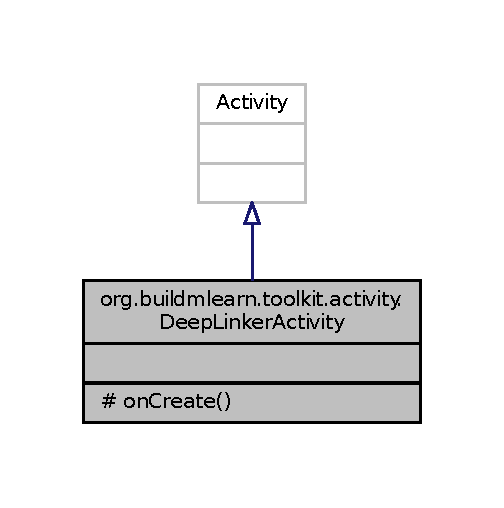
\includegraphics[width=242pt]{d6/d40/classorg_1_1buildmlearn_1_1toolkit_1_1activity_1_1DeepLinkerActivity__inherit__graph}
\end{center}
\end{figure}


Collaboration diagram for org.\-buildmlearn.\-toolkit.\-activity.\-Deep\-Linker\-Activity\-:
\nopagebreak
\begin{figure}[H]
\begin{center}
\leavevmode
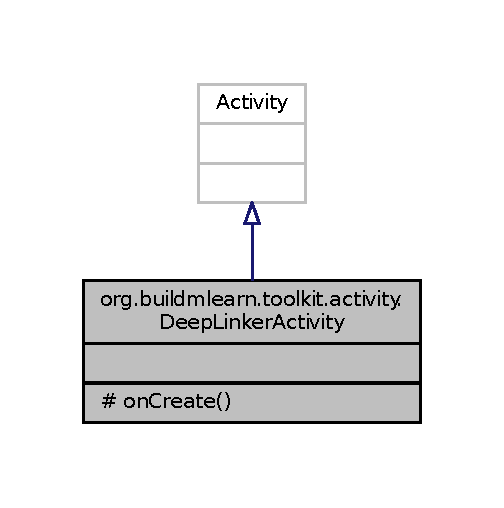
\includegraphics[width=242pt]{de/dab/classorg_1_1buildmlearn_1_1toolkit_1_1activity_1_1DeepLinkerActivity__coll__graph}
\end{center}
\end{figure}
\subsection*{Protected Member Functions}
\begin{DoxyCompactItemize}
\item 
void \hyperlink{classorg_1_1buildmlearn_1_1toolkit_1_1activity_1_1DeepLinkerActivity_a7737f816c7d10e707b4788bf5ae2f591}{on\-Create} (Bundle saved\-Instance\-State)
\end{DoxyCompactItemize}


\subsection{Detailed Description}
Activity responsible for handling files opened from file explorer. 

This activity is started whenever users opens a .buildmlearn file from file explorer. This activity is responsible for getting the template type from the file, and passes the template Id and file path to Template Editor/ activity. 

\subsection{Member Function Documentation}
\hypertarget{classorg_1_1buildmlearn_1_1toolkit_1_1activity_1_1DeepLinkerActivity_a7737f816c7d10e707b4788bf5ae2f591}{\index{org\-::buildmlearn\-::toolkit\-::activity\-::\-Deep\-Linker\-Activity@{org\-::buildmlearn\-::toolkit\-::activity\-::\-Deep\-Linker\-Activity}!on\-Create@{on\-Create}}
\index{on\-Create@{on\-Create}!org::buildmlearn::toolkit::activity::DeepLinkerActivity@{org\-::buildmlearn\-::toolkit\-::activity\-::\-Deep\-Linker\-Activity}}
\subsubsection[{on\-Create}]{\setlength{\rightskip}{0pt plus 5cm}void org.\-buildmlearn.\-toolkit.\-activity.\-Deep\-Linker\-Activity.\-on\-Create (
\begin{DoxyParamCaption}
\item[{Bundle}]{saved\-Instance\-State}
\end{DoxyParamCaption}
)\hspace{0.3cm}{\ttfamily [protected]}}}\label{classorg_1_1buildmlearn_1_1toolkit_1_1activity_1_1DeepLinkerActivity_a7737f816c7d10e707b4788bf5ae2f591}

\begin{DoxyCode}
36                                                        \{
37         super.onCreate(savedInstanceState);
38         Uri data = getIntent().getData();
39         File fXmlFile = \textcolor{keyword}{new} File(data.getPath());
40 
41         DocumentBuilderFactory dbFactory = DocumentBuilderFactory.newInstance();
42         DocumentBuilder dBuilder;
43         \textcolor{keywordflow}{try} \{
44             dBuilder = dbFactory.newDocumentBuilder();
45             Document doc = dBuilder.parse(fXmlFile);
46             doc.getDocumentElement().normalize();
47             Log.d(\textcolor{stringliteral}{"Files"}, \textcolor{stringliteral}{"Root element :"} + doc.getDocumentElement().getAttribute(\textcolor{stringliteral}{"type"}));
48             SavedProject savedProject = \textcolor{keyword}{new} SavedProject(fXmlFile, fXmlFile.getName(), 
      fXmlFile.lastModified(), doc.getDocumentElement().getAttribute(\textcolor{stringliteral}{"type"}), fXmlFile.getAbsolutePath());
49             Template[] templates = Template.values();
50             \textcolor{keywordflow}{for} (\textcolor{keywordtype}{int} i = 0; i < templates.length; i++) \{
51                 \textcolor{keywordflow}{if} (savedProject.getType().equals(getString(templates[i].getType()))) \{
52                     Intent intent = \textcolor{keyword}{new} Intent(\textcolor{keyword}{this}, TemplateEditor.class);
53                     intent.putExtra(\hyperlink{classorg_1_1buildmlearn_1_1toolkit_1_1constant_1_1Constants_a2ee9d59d6a353dc4664ed2e2086dae9d}{Constants.TEMPLATE\_ID}, i);
54                     intent.putExtra(\hyperlink{classorg_1_1buildmlearn_1_1toolkit_1_1constant_1_1Constants_ab2586e8aa144cd7e8b4928186d709ea8}{Constants.PROJECT\_FILE\_PATH}, 
      savedProject.getFullPath());
55                     startActivity(intent);
56                     finish();
57                     \textcolor{keywordflow}{return};
58                 \}
59             \}
60             Toast.makeText(\textcolor{keyword}{this}, \textcolor{stringliteral}{"Invalid project file"}, Toast.LENGTH\_SHORT).show();
61             finish();
62         \} \textcolor{keywordflow}{catch} (ParserConfigurationException e) \{
63             e.printStackTrace();
64         \} \textcolor{keywordflow}{catch} (SAXException e) \{
65             e.printStackTrace();
66         \} \textcolor{keywordflow}{catch} (IOException e) \{
67             e.printStackTrace();
68         \}
69     \}
\end{DoxyCode}


The documentation for this class was generated from the following file\-:\begin{DoxyCompactItemize}
\item 
/\-Buildm\-Learn-\/\-Toolkit-\/\-Android/source-\/code/app/src/main/java/org/buildmlearn/toolkit/activity/\hyperlink{DeepLinkerActivity_8java}{Deep\-Linker\-Activity.\-java}\end{DoxyCompactItemize}

\hypertarget{classorg_1_1buildmlearn_1_1toolkit_1_1infotemplate_1_1DetailView}{\section{org.\-buildmlearn.\-toolkit.\-infotemplate.\-Detail\-View Class Reference}
\label{classorg_1_1buildmlearn_1_1toolkit_1_1infotemplate_1_1DetailView}\index{org.\-buildmlearn.\-toolkit.\-infotemplate.\-Detail\-View@{org.\-buildmlearn.\-toolkit.\-infotemplate.\-Detail\-View}}
}


Simulator code for Info Template.  




Inheritance diagram for org.\-buildmlearn.\-toolkit.\-infotemplate.\-Detail\-View\-:
\nopagebreak
\begin{figure}[H]
\begin{center}
\leavevmode
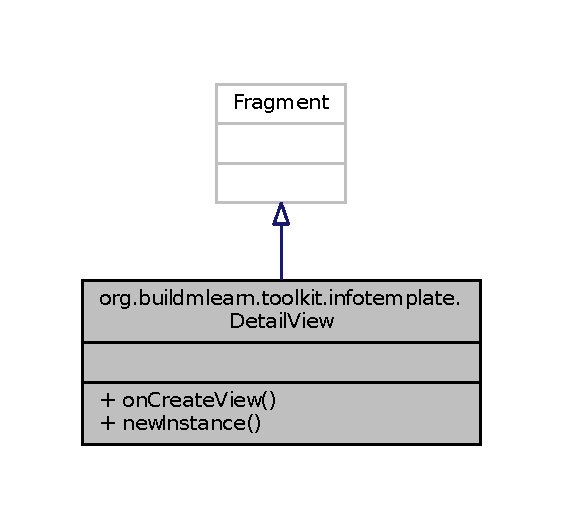
\includegraphics[width=270pt]{da/d98/classorg_1_1buildmlearn_1_1toolkit_1_1infotemplate_1_1DetailView__inherit__graph}
\end{center}
\end{figure}


Collaboration diagram for org.\-buildmlearn.\-toolkit.\-infotemplate.\-Detail\-View\-:
\nopagebreak
\begin{figure}[H]
\begin{center}
\leavevmode
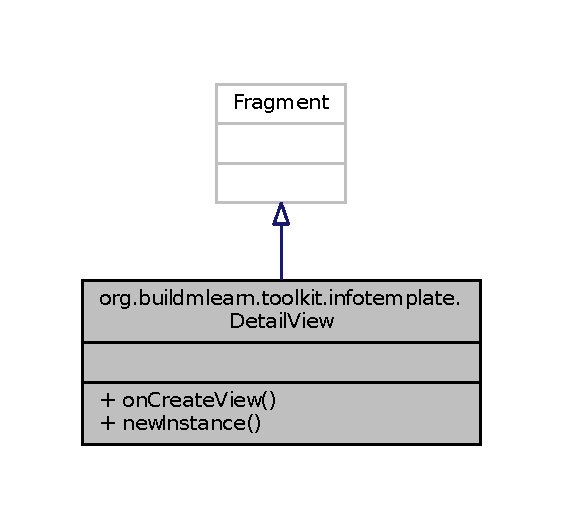
\includegraphics[width=270pt]{d7/d10/classorg_1_1buildmlearn_1_1toolkit_1_1infotemplate_1_1DetailView__coll__graph}
\end{center}
\end{figure}
\subsection*{Public Member Functions}
\begin{DoxyCompactItemize}
\item 
View \hyperlink{classorg_1_1buildmlearn_1_1toolkit_1_1infotemplate_1_1DetailView_a6a003850a5524fee3987264baaabf903}{on\-Create\-View} (Layout\-Inflater inflater, View\-Group container, Bundle saved\-Instance\-State)
\end{DoxyCompactItemize}
\subsection*{Static Public Member Functions}
\begin{DoxyCompactItemize}
\item 
static Fragment \hyperlink{classorg_1_1buildmlearn_1_1toolkit_1_1infotemplate_1_1DetailView_a9402197a3f6fcc0b4c3cb365ae452bf3}{new\-Instance} (int position)
\end{DoxyCompactItemize}


\subsection{Detailed Description}
Simulator code for Info Template. 

\subsection{Member Function Documentation}
\hypertarget{classorg_1_1buildmlearn_1_1toolkit_1_1infotemplate_1_1DetailView_a9402197a3f6fcc0b4c3cb365ae452bf3}{\index{org\-::buildmlearn\-::toolkit\-::infotemplate\-::\-Detail\-View@{org\-::buildmlearn\-::toolkit\-::infotemplate\-::\-Detail\-View}!new\-Instance@{new\-Instance}}
\index{new\-Instance@{new\-Instance}!org::buildmlearn::toolkit::infotemplate::DetailView@{org\-::buildmlearn\-::toolkit\-::infotemplate\-::\-Detail\-View}}
\subsubsection[{new\-Instance}]{\setlength{\rightskip}{0pt plus 5cm}static Fragment org.\-buildmlearn.\-toolkit.\-infotemplate.\-Detail\-View.\-new\-Instance (
\begin{DoxyParamCaption}
\item[{int}]{position}
\end{DoxyParamCaption}
)\hspace{0.3cm}{\ttfamily [static]}}}\label{classorg_1_1buildmlearn_1_1toolkit_1_1infotemplate_1_1DetailView_a9402197a3f6fcc0b4c3cb365ae452bf3}

\begin{DoxyCode}
73                                                      \{
74         DetailView fragment = \textcolor{keyword}{new} DetailView();
75         Bundle bundle = \textcolor{keyword}{new} Bundle();
76         bundle.putInt(\textcolor{stringliteral}{"position"}, position);
77         fragment.setArguments(bundle);
78         \textcolor{keywordflow}{return} fragment;
79     \}
\end{DoxyCode}
\hypertarget{classorg_1_1buildmlearn_1_1toolkit_1_1infotemplate_1_1DetailView_a6a003850a5524fee3987264baaabf903}{\index{org\-::buildmlearn\-::toolkit\-::infotemplate\-::\-Detail\-View@{org\-::buildmlearn\-::toolkit\-::infotemplate\-::\-Detail\-View}!on\-Create\-View@{on\-Create\-View}}
\index{on\-Create\-View@{on\-Create\-View}!org::buildmlearn::toolkit::infotemplate::DetailView@{org\-::buildmlearn\-::toolkit\-::infotemplate\-::\-Detail\-View}}
\subsubsection[{on\-Create\-View}]{\setlength{\rightskip}{0pt plus 5cm}View org.\-buildmlearn.\-toolkit.\-infotemplate.\-Detail\-View.\-on\-Create\-View (
\begin{DoxyParamCaption}
\item[{Layout\-Inflater}]{inflater, }
\item[{View\-Group}]{container, }
\item[{Bundle}]{saved\-Instance\-State}
\end{DoxyParamCaption}
)}}\label{classorg_1_1buildmlearn_1_1toolkit_1_1infotemplate_1_1DetailView_a6a003850a5524fee3987264baaabf903}

\begin{DoxyCode}
83                                                                                                       \{
84 
85         View view = inflater.inflate(R.layout.info\_template\_detail, container, \textcolor{keyword}{false});
86         TextView title = (TextView) view.findViewById(R.id.titleText);
87         TextView details = (TextView) view.findViewById(R.id.detailText);
88         \textcolor{keywordtype}{int} position = getArguments().getInt(\textcolor{stringliteral}{"position"}, 0);
89         InfoModel model = GlobalData.getInstance().mList.get(position);
90         title.setText(model.getInfo\_object());
91         details.setText(model.getInfo\_description());
92         view.findViewById(R.id.info\_template\_simulator\_back\_button).setOnClickListener(\textcolor{keyword}{new} View.
      OnClickListener() \{
93             @Override
94             \textcolor{keyword}{public} \textcolor{keywordtype}{void} onClick(View v) \{
95 
96                 getActivity().getFragmentManager().popBackStack();
97 
98             \}
99         \});
100         \textcolor{keywordflow}{return} view;
101     \}
\end{DoxyCode}


The documentation for this class was generated from the following file\-:\begin{DoxyCompactItemize}
\item 
/\-Buildm\-Learn-\/\-Toolkit-\/\-Android/source-\/code/app/src/main/java/org/buildmlearn/toolkit/infotemplate/\hyperlink{DetailView_8java}{Detail\-View.\-java}\end{DoxyCompactItemize}

\hypertarget{classorg_1_1buildmlearn_1_1toolkit_1_1utilities_1_1FileUtils}{\section{org.\-buildmlearn.\-toolkit.\-utilities.\-File\-Utils Class Reference}
\label{classorg_1_1buildmlearn_1_1toolkit_1_1utilities_1_1FileUtils}\index{org.\-buildmlearn.\-toolkit.\-utilities.\-File\-Utils@{org.\-buildmlearn.\-toolkit.\-utilities.\-File\-Utils}}
}


Helper functions related to String manipulation.  




Collaboration diagram for org.\-buildmlearn.\-toolkit.\-utilities.\-File\-Utils\-:
\nopagebreak
\begin{figure}[H]
\begin{center}
\leavevmode
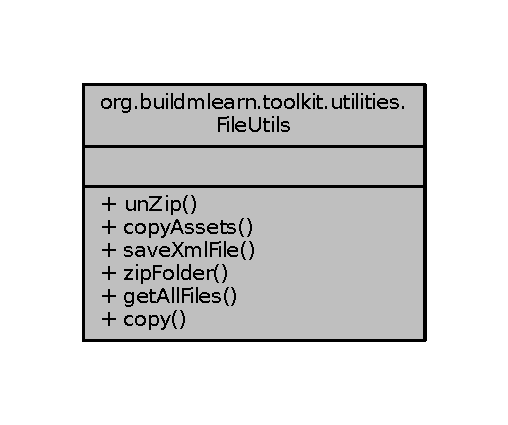
\includegraphics[width=244pt]{d4/d37/classorg_1_1buildmlearn_1_1toolkit_1_1utilities_1_1FileUtils__coll__graph}
\end{center}
\end{figure}
\subsection*{Static Public Member Functions}
\begin{DoxyCompactItemize}
\item 
static void \hyperlink{classorg_1_1buildmlearn_1_1toolkit_1_1utilities_1_1FileUtils_a3985505c7367639777e7829b87fa625b}{un\-Zip} (String zip\-File\-Path, String destination\-Folder)  throws I\-O\-Exception 
\begin{DoxyCompactList}\small\item\em Unzips a compressed file (.zip, .apk) \end{DoxyCompactList}\item 
static void \hyperlink{classorg_1_1buildmlearn_1_1toolkit_1_1utilities_1_1FileUtils_a40211ea6f81fcdd275cb33047c67c01a}{copy\-Assets} (Context context, String asset\-File\-Name, String destination\-Directory)
\begin{DoxyCompactList}\small\item\em Copies a file from assets folder to a folder on device memory. \end{DoxyCompactList}\item 
static boolean \hyperlink{classorg_1_1buildmlearn_1_1toolkit_1_1utilities_1_1FileUtils_a37f577c0b56f2ffc56824657ac220fb7}{save\-Xml\-File} (String destination\-Folder, String file\-Name, Document doc)
\begin{DoxyCompactList}\small\item\em Converts a given Document object to xml format file. \end{DoxyCompactList}\item 
static void \hyperlink{classorg_1_1buildmlearn_1_1toolkit_1_1utilities_1_1FileUtils_aa79713cc1d17fbf9b7294c60e851b774}{zip\-Folder} (String directory\-To\-Zip\-Path)  throws I\-O\-Exception 
\begin{DoxyCompactList}\small\item\em Archives a folder into .zip compressed file. \end{DoxyCompactList}\item 
static void \hyperlink{classorg_1_1buildmlearn_1_1toolkit_1_1utilities_1_1FileUtils_aa61e000a3890f6d8b42c1a537f8c2df4}{get\-All\-Files} (File dir, List$<$ File $>$ file\-List)
\begin{DoxyCompactList}\small\item\em Add all the files in a given folder into a list. \end{DoxyCompactList}\item 
static void \hyperlink{classorg_1_1buildmlearn_1_1toolkit_1_1utilities_1_1FileUtils_a22131f5eeefec02f52908ab439ab528b}{copy} (File src, File dst)  throws I\-O\-Exception 
\begin{DoxyCompactList}\small\item\em Copies the content from one file to another. \end{DoxyCompactList}\end{DoxyCompactItemize}


\subsection{Detailed Description}
Helper functions related to String manipulation. 

Created by Abhishek on 23-\/05-\/2015. 

\subsection{Member Function Documentation}
\hypertarget{classorg_1_1buildmlearn_1_1toolkit_1_1utilities_1_1FileUtils_a22131f5eeefec02f52908ab439ab528b}{\index{org\-::buildmlearn\-::toolkit\-::utilities\-::\-File\-Utils@{org\-::buildmlearn\-::toolkit\-::utilities\-::\-File\-Utils}!copy@{copy}}
\index{copy@{copy}!org::buildmlearn::toolkit::utilities::FileUtils@{org\-::buildmlearn\-::toolkit\-::utilities\-::\-File\-Utils}}
\subsubsection[{copy}]{\setlength{\rightskip}{0pt plus 5cm}static void org.\-buildmlearn.\-toolkit.\-utilities.\-File\-Utils.\-copy (
\begin{DoxyParamCaption}
\item[{File}]{src, }
\item[{File}]{dst}
\end{DoxyParamCaption}
) throws I\-O\-Exception\hspace{0.3cm}{\ttfamily [static]}}}\label{classorg_1_1buildmlearn_1_1toolkit_1_1utilities_1_1FileUtils_a22131f5eeefec02f52908ab439ab528b}


Copies the content from one file to another. 


\begin{DoxyParams}{Parameters}
{\em src} & Source file \\
\hline
{\em dst} & Destination file \\
\hline
\end{DoxyParams}

\begin{DoxyExceptions}{Exceptions}
{\em I\-O\-Exception} & Exception thrown in case of error \\
\hline
\end{DoxyExceptions}

\begin{DoxyCode}
257                                                                    \{
258         InputStream in = \textcolor{keyword}{new} FileInputStream(src);
259         OutputStream out = \textcolor{keyword}{new} FileOutputStream(dst);
260 
261         \textcolor{comment}{// Transfer bytes from in to out}
262         byte[] buf = \textcolor{keyword}{new} byte[1024];
263         \textcolor{keywordtype}{int} len;
264         \textcolor{keywordflow}{while} ((len = in.read(buf)) > 0) \{
265             out.write(buf, 0, len);
266         \}
267         in.close();
268         out.close();
269     \}
\end{DoxyCode}
\hypertarget{classorg_1_1buildmlearn_1_1toolkit_1_1utilities_1_1FileUtils_a40211ea6f81fcdd275cb33047c67c01a}{\index{org\-::buildmlearn\-::toolkit\-::utilities\-::\-File\-Utils@{org\-::buildmlearn\-::toolkit\-::utilities\-::\-File\-Utils}!copy\-Assets@{copy\-Assets}}
\index{copy\-Assets@{copy\-Assets}!org::buildmlearn::toolkit::utilities::FileUtils@{org\-::buildmlearn\-::toolkit\-::utilities\-::\-File\-Utils}}
\subsubsection[{copy\-Assets}]{\setlength{\rightskip}{0pt plus 5cm}static void org.\-buildmlearn.\-toolkit.\-utilities.\-File\-Utils.\-copy\-Assets (
\begin{DoxyParamCaption}
\item[{Context}]{context, }
\item[{String}]{asset\-File\-Name, }
\item[{String}]{destination\-Directory}
\end{DoxyParamCaption}
)\hspace{0.3cm}{\ttfamily [static]}}}\label{classorg_1_1buildmlearn_1_1toolkit_1_1utilities_1_1FileUtils_a40211ea6f81fcdd275cb33047c67c01a}


Copies a file from assets folder to a folder on device memory. 


\begin{DoxyParams}{Parameters}
{\em context} & Application context \\
\hline
{\em asset\-File\-Name} & Name of the file stored in assets \\
\hline
{\em destination\-Directory} & Destination folder for saving the file \\
\hline
\end{DoxyParams}

\begin{DoxyCode}
108                                                                                                       \{
109         AssetManager assetManager = context.getAssets();
110         InputStream in;
111         OutputStream out;
112         \textcolor{keywordflow}{try} \{
113             in = assetManager.open(assetFileName);
114             String outPutPath = destinationDirectory;
115             File f = \textcolor{keyword}{new} File(outPutPath);
116             \textcolor{keywordflow}{if} (!f.isDirectory()) \{
117                 f.mkdirs();
118             \}
119 
120             File outFile = \textcolor{keyword}{new} File(outPutPath, assetFileName);
121             out = \textcolor{keyword}{new} FileOutputStream(outFile);
122             copyFile(in, out);
123             in.close();
124             out.flush();
125             out.close();
126         \} \textcolor{keywordflow}{catch} (IOException e) \{
127             e.printStackTrace();
128         \}
129 
130     \}
\end{DoxyCode}
\hypertarget{classorg_1_1buildmlearn_1_1toolkit_1_1utilities_1_1FileUtils_aa61e000a3890f6d8b42c1a537f8c2df4}{\index{org\-::buildmlearn\-::toolkit\-::utilities\-::\-File\-Utils@{org\-::buildmlearn\-::toolkit\-::utilities\-::\-File\-Utils}!get\-All\-Files@{get\-All\-Files}}
\index{get\-All\-Files@{get\-All\-Files}!org::buildmlearn::toolkit::utilities::FileUtils@{org\-::buildmlearn\-::toolkit\-::utilities\-::\-File\-Utils}}
\subsubsection[{get\-All\-Files}]{\setlength{\rightskip}{0pt plus 5cm}static void org.\-buildmlearn.\-toolkit.\-utilities.\-File\-Utils.\-get\-All\-Files (
\begin{DoxyParamCaption}
\item[{File}]{dir, }
\item[{List$<$ File $>$}]{file\-List}
\end{DoxyParamCaption}
)\hspace{0.3cm}{\ttfamily [static]}}}\label{classorg_1_1buildmlearn_1_1toolkit_1_1utilities_1_1FileUtils_aa61e000a3890f6d8b42c1a537f8c2df4}


Add all the files in a given folder into a list. 


\begin{DoxyParams}{Parameters}
{\em dir} & Source directory \\
\hline
{\em file\-List} & Referenced list. Files are added to this list \\
\hline
\end{DoxyParams}

\begin{DoxyCode}
190                                                                   \{
191         \textcolor{keywordflow}{try} \{
192             File[] files = dir.listFiles();
193             \textcolor{keywordflow}{for} (File file : files) \{
194                 fileList.add(file);
195                 \textcolor{keywordflow}{if} (file.isDirectory()) \{
196                     System.out.println(\textcolor{stringliteral}{"directory:"} + file.getCanonicalPath());
197                     \hyperlink{classorg_1_1buildmlearn_1_1toolkit_1_1utilities_1_1FileUtils_aa61e000a3890f6d8b42c1a537f8c2df4}{getAllFiles}(file, fileList);
198                 \} \textcolor{keywordflow}{else} \{
199                     System.out.println(\textcolor{stringliteral}{"     file:"} + file.getCanonicalPath());
200                 \}
201             \}
202         \} \textcolor{keywordflow}{catch} (IOException e) \{
203             e.printStackTrace();
204         \}
205     \}
\end{DoxyCode}
\hypertarget{classorg_1_1buildmlearn_1_1toolkit_1_1utilities_1_1FileUtils_a37f577c0b56f2ffc56824657ac220fb7}{\index{org\-::buildmlearn\-::toolkit\-::utilities\-::\-File\-Utils@{org\-::buildmlearn\-::toolkit\-::utilities\-::\-File\-Utils}!save\-Xml\-File@{save\-Xml\-File}}
\index{save\-Xml\-File@{save\-Xml\-File}!org::buildmlearn::toolkit::utilities::FileUtils@{org\-::buildmlearn\-::toolkit\-::utilities\-::\-File\-Utils}}
\subsubsection[{save\-Xml\-File}]{\setlength{\rightskip}{0pt plus 5cm}static boolean org.\-buildmlearn.\-toolkit.\-utilities.\-File\-Utils.\-save\-Xml\-File (
\begin{DoxyParamCaption}
\item[{String}]{destination\-Folder, }
\item[{String}]{file\-Name, }
\item[{Document}]{doc}
\end{DoxyParamCaption}
)\hspace{0.3cm}{\ttfamily [static]}}}\label{classorg_1_1buildmlearn_1_1toolkit_1_1utilities_1_1FileUtils_a37f577c0b56f2ffc56824657ac220fb7}


Converts a given Document object to xml format file. 


\begin{DoxyParams}{Parameters}
{\em destination\-Folder} & Destination folder for saving the file \\
\hline
{\em file\-Name} & Destination file name \\
\hline
{\em doc} & Document object to be converted to xml formatted file \\
\hline
\end{DoxyParams}
\begin{DoxyReturn}{Returns}
Returns true if successfully converted 
\end{DoxyReturn}

\begin{DoxyCode}
147                                                                                                \{
148 
149         File f = \textcolor{keyword}{new} File(destinationFolder);
150         \textcolor{keywordflow}{if} (!f.isDirectory()) \{
151             f.mkdirs();
152         \}
153         TransformerFactory transformerFactory = TransformerFactory.newInstance();
154         Transformer transformer;
155         \textcolor{keywordflow}{try} \{
156             transformer = transformerFactory.newTransformer();
157             DOMSource source = \textcolor{keyword}{new} DOMSource(doc);
158             StreamResult result = \textcolor{keyword}{new} StreamResult(\textcolor{keyword}{new} File(destinationFolder + fileName));
159             transformer.transform(source, result);
160             \textcolor{keywordflow}{return} \textcolor{keyword}{true};
161         \} \textcolor{keywordflow}{catch} (TransformerConfigurationException e) \{
162             e.printStackTrace();
163         \} \textcolor{keywordflow}{catch} (TransformerException e) \{
164             e.printStackTrace();
165         \}
166         \textcolor{keywordflow}{return} \textcolor{keyword}{false};
167     \}
\end{DoxyCode}
\hypertarget{classorg_1_1buildmlearn_1_1toolkit_1_1utilities_1_1FileUtils_a3985505c7367639777e7829b87fa625b}{\index{org\-::buildmlearn\-::toolkit\-::utilities\-::\-File\-Utils@{org\-::buildmlearn\-::toolkit\-::utilities\-::\-File\-Utils}!un\-Zip@{un\-Zip}}
\index{un\-Zip@{un\-Zip}!org::buildmlearn::toolkit::utilities::FileUtils@{org\-::buildmlearn\-::toolkit\-::utilities\-::\-File\-Utils}}
\subsubsection[{un\-Zip}]{\setlength{\rightskip}{0pt plus 5cm}static void org.\-buildmlearn.\-toolkit.\-utilities.\-File\-Utils.\-un\-Zip (
\begin{DoxyParamCaption}
\item[{String}]{zip\-File\-Path, }
\item[{String}]{destination\-Folder}
\end{DoxyParamCaption}
) throws I\-O\-Exception\hspace{0.3cm}{\ttfamily [static]}}}\label{classorg_1_1buildmlearn_1_1toolkit_1_1utilities_1_1FileUtils_a3985505c7367639777e7829b87fa625b}


Unzips a compressed file (.zip, .apk) 


\begin{DoxyParams}{Parameters}
{\em zip\-File\-Path} & Path of the source zip file \\
\hline
{\em destination\-Folder} & Destination folder for stroing the uncompresses files. \\
\hline
\end{DoxyParams}

\begin{DoxyExceptions}{Exceptions}
{\em I\-O\-Exception} & Exception thrown in case of some error. \\
\hline
\end{DoxyExceptions}

\begin{DoxyCode}
48                                                                                               \{
49         \textcolor{keywordtype}{int} size;
50         byte[] buffer = \textcolor{keyword}{new} byte[BUFFER\_SIZE];
51         \textcolor{keywordflow}{try} \{
52             \textcolor{keywordflow}{if} (!destinationFolder.endsWith(\textcolor{stringliteral}{"/"})) \{
53                 destinationFolder += \textcolor{stringliteral}{"/"};
54             \}
55             File f = \textcolor{keyword}{new} File(destinationFolder);
56             \textcolor{keywordflow}{if} (!f.isDirectory()) \{
57                 f.mkdirs();
58             \}
59 
60             ZipInputStream zin = \textcolor{keyword}{new} ZipInputStream(\textcolor{keyword}{new} BufferedInputStream(\textcolor{keyword}{new} FileInputStream(zipFilePath
      ), BUFFER\_SIZE));
61             \textcolor{keywordflow}{try} \{
62                 ZipEntry ze;
63                 \textcolor{keywordflow}{while} ((ze = zin.getNextEntry()) != null) \{
64                     String path = destinationFolder + ze.getName();
65                     File unzipFile = \textcolor{keyword}{new} File(path);
66 
67                     \textcolor{keywordflow}{if} (ze.isDirectory()) \{
68                         \textcolor{keywordflow}{if} (!unzipFile.isDirectory()) \{
69                             unzipFile.mkdirs();
70                         \}
71                     \} \textcolor{keywordflow}{else} \{
72 
73                         File parentDir = unzipFile.getParentFile();
74                         \textcolor{keywordflow}{if} (null != parentDir) \{
75                             \textcolor{keywordflow}{if} (!parentDir.isDirectory()) \{
76                                 parentDir.mkdirs();
77                             \}
78                         \}
79 
80                         FileOutputStream out = \textcolor{keyword}{new} FileOutputStream(unzipFile, \textcolor{keyword}{false});
81                         BufferedOutputStream fout = \textcolor{keyword}{new} BufferedOutputStream(out, BUFFER\_SIZE);
82                         \textcolor{keywordflow}{try} \{
83                             \textcolor{keywordflow}{while} ((size = zin.read(buffer, 0, BUFFER\_SIZE)) != -1) \{
84                                 fout.write(buffer, 0, size);
85                             \}
86 
87                             zin.closeEntry();
88                         \} \textcolor{keywordflow}{finally} \{
89                             fout.flush();
90                             fout.close();
91                         \}
92                     \}
93                 \}
94             \} \textcolor{keywordflow}{finally} \{
95                 zin.close();
96             \}
97         \} \textcolor{keywordflow}{catch} (Exception e) \{
98             e.printStackTrace();
99         \}
100     \}
\end{DoxyCode}
\hypertarget{classorg_1_1buildmlearn_1_1toolkit_1_1utilities_1_1FileUtils_aa79713cc1d17fbf9b7294c60e851b774}{\index{org\-::buildmlearn\-::toolkit\-::utilities\-::\-File\-Utils@{org\-::buildmlearn\-::toolkit\-::utilities\-::\-File\-Utils}!zip\-Folder@{zip\-Folder}}
\index{zip\-Folder@{zip\-Folder}!org::buildmlearn::toolkit::utilities::FileUtils@{org\-::buildmlearn\-::toolkit\-::utilities\-::\-File\-Utils}}
\subsubsection[{zip\-Folder}]{\setlength{\rightskip}{0pt plus 5cm}static void org.\-buildmlearn.\-toolkit.\-utilities.\-File\-Utils.\-zip\-Folder (
\begin{DoxyParamCaption}
\item[{String}]{directory\-To\-Zip\-Path}
\end{DoxyParamCaption}
) throws I\-O\-Exception\hspace{0.3cm}{\ttfamily [static]}}}\label{classorg_1_1buildmlearn_1_1toolkit_1_1utilities_1_1FileUtils_aa79713cc1d17fbf9b7294c60e851b774}


Archives a folder into .zip compressed file. 


\begin{DoxyParams}{Parameters}
{\em directory\-To\-Zip\-Path} & Source folder to be converted. \\
\hline
\end{DoxyParams}

\begin{DoxyExceptions}{Exceptions}
{\em I\-O\-Exception} & \\
\hline
\end{DoxyExceptions}

\begin{DoxyCode}
174                                                                                \{
175         File directoryToZip = \textcolor{keyword}{new} File(directoryToZipPath);
176 
177         List<File> fileList = \textcolor{keyword}{new} ArrayList<File>();
178         System.out.println(\textcolor{stringliteral}{"---Getting references to all files in: "} + directoryToZip.getCanonicalPath());
179         \hyperlink{classorg_1_1buildmlearn_1_1toolkit_1_1utilities_1_1FileUtils_aa61e000a3890f6d8b42c1a537f8c2df4}{getAllFiles}(directoryToZip, fileList);
180         System.out.println(\textcolor{stringliteral}{"---Creating zip file"});
181         writeZipFile(directoryToZip, fileList);
182         System.out.println(\textcolor{stringliteral}{"---Done"});
183     \}
\end{DoxyCode}


The documentation for this class was generated from the following file\-:\begin{DoxyCompactItemize}
\item 
/\-Buildm\-Learn-\/\-Toolkit-\/\-Android/source-\/code/app/src/main/java/org/buildmlearn/toolkit/utilities/\hyperlink{FileUtils_8java}{File\-Utils.\-java}\end{DoxyCompactItemize}

\hypertarget{classorg_1_1buildmlearn_1_1toolkit_1_1activity_1_1FirstRunActivity}{\section{org.\-buildmlearn.\-toolkit.\-activity.\-First\-Run\-Activity Class Reference}
\label{classorg_1_1buildmlearn_1_1toolkit_1_1activity_1_1FirstRunActivity}\index{org.\-buildmlearn.\-toolkit.\-activity.\-First\-Run\-Activity@{org.\-buildmlearn.\-toolkit.\-activity.\-First\-Run\-Activity}}
}


Shown on application first launch.  




Inheritance diagram for org.\-buildmlearn.\-toolkit.\-activity.\-First\-Run\-Activity\-:
\nopagebreak
\begin{figure}[H]
\begin{center}
\leavevmode
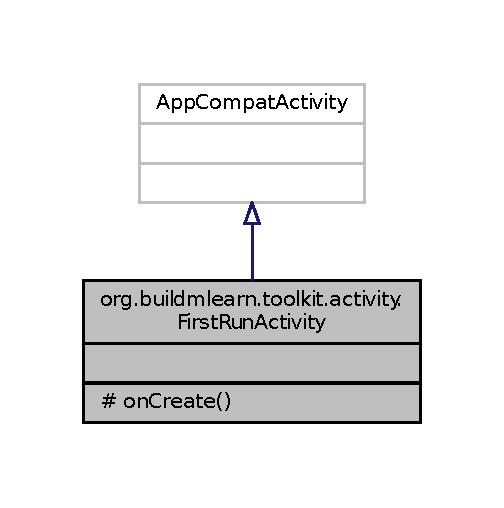
\includegraphics[width=242pt]{d7/d56/classorg_1_1buildmlearn_1_1toolkit_1_1activity_1_1FirstRunActivity__inherit__graph}
\end{center}
\end{figure}


Collaboration diagram for org.\-buildmlearn.\-toolkit.\-activity.\-First\-Run\-Activity\-:
\nopagebreak
\begin{figure}[H]
\begin{center}
\leavevmode
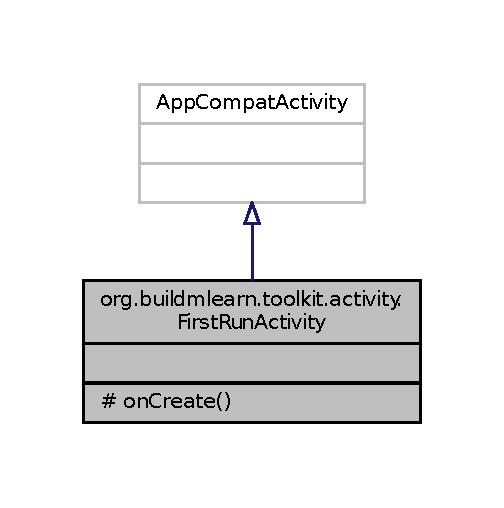
\includegraphics[width=242pt]{d1/d9d/classorg_1_1buildmlearn_1_1toolkit_1_1activity_1_1FirstRunActivity__coll__graph}
\end{center}
\end{figure}
\subsection*{Protected Member Functions}
\begin{DoxyCompactItemize}
\item 
void \hyperlink{classorg_1_1buildmlearn_1_1toolkit_1_1activity_1_1FirstRunActivity_a847a7bc25bdbd77b2a7bc90cd3ca38bb}{on\-Create} (Bundle saved\-Instance\-State)
\end{DoxyCompactItemize}


\subsection{Detailed Description}
Shown on application first launch. 

\subsection{Member Function Documentation}
\hypertarget{classorg_1_1buildmlearn_1_1toolkit_1_1activity_1_1FirstRunActivity_a847a7bc25bdbd77b2a7bc90cd3ca38bb}{\index{org\-::buildmlearn\-::toolkit\-::activity\-::\-First\-Run\-Activity@{org\-::buildmlearn\-::toolkit\-::activity\-::\-First\-Run\-Activity}!on\-Create@{on\-Create}}
\index{on\-Create@{on\-Create}!org::buildmlearn::toolkit::activity::FirstRunActivity@{org\-::buildmlearn\-::toolkit\-::activity\-::\-First\-Run\-Activity}}
\subsubsection[{on\-Create}]{\setlength{\rightskip}{0pt plus 5cm}void org.\-buildmlearn.\-toolkit.\-activity.\-First\-Run\-Activity.\-on\-Create (
\begin{DoxyParamCaption}
\item[{Bundle}]{saved\-Instance\-State}
\end{DoxyParamCaption}
)\hspace{0.3cm}{\ttfamily [protected]}}}\label{classorg_1_1buildmlearn_1_1toolkit_1_1activity_1_1FirstRunActivity_a847a7bc25bdbd77b2a7bc90cd3ca38bb}

\begin{DoxyCode}
33                                                        \{
34         super.onCreate(savedInstanceState);
35         prefs = PreferenceManager.getDefaultSharedPreferences(getApplicationContext());
36 
37         \textcolor{keywordflow}{if} (prefs.getBoolean(FIRST\_RUN, \textcolor{keyword}{false})) \{
38             startActivity(\textcolor{keyword}{new} Intent(getApplicationContext(), HomeActivity.class));
39             finish();
40         \}
41         setContentView(R.layout.activity\_first\_run);
42 
43 
44         findViewById(R.id.focus\_thief).clearFocus();
45         YoYo.with(Techniques.BounceInUp)
46                 .duration(2700)
47                 .playOn(findViewById(R.id.first\_name));
48 
49 
50         name = (EditText) findViewById(R.id.first\_name);
51 
52 
53         name.setOnKeyListener(\textcolor{keyword}{new} View.OnKeyListener() \{
54             @Override
55             \textcolor{keyword}{public} \textcolor{keywordtype}{boolean} onKey(View v, \textcolor{keywordtype}{int} keyCode, KeyEvent event) \{
56                 \textcolor{keywordflow}{if} (event.getAction() == KeyEvent.ACTION\_DOWN) \{
57                     \textcolor{keywordflow}{switch} (keyCode) \{
58                         \textcolor{keywordflow}{case} KeyEvent.KEYCODE\_DPAD\_CENTER:
59                         \textcolor{keywordflow}{case} KeyEvent.KEYCODE\_ENTER:
60 
61                             \textcolor{keywordflow}{if} (name.getText().toString().equals(\textcolor{stringliteral}{""})) \{
62                                 Toast.makeText(getApplicationContext(), \textcolor{stringliteral}{"Enter name"}, Toast.LENGTH\_SHORT).
      show();
63                                 \textcolor{keywordflow}{return} \textcolor{keyword}{false};
64                             \}
65 
66 
67                             SharedPreferences.Editor editor = prefs.edit();
68 
69                             editor.putString(getString(R.string.key\_user\_name), name.getText().toString());
70                             editor.putBoolean(FIRST\_RUN, \textcolor{keyword}{true});
71                             editor.commit();
72                             Intent intent = \textcolor{keyword}{new} Intent(getApplicationContext(), TutorialActivity.class);
73                             intent.putExtra(\hyperlink{classorg_1_1buildmlearn_1_1toolkit_1_1constant_1_1Constants_a2799e097282009a747db0225f72508ff}{Constants.START\_ACTIVITY}, \textcolor{keyword}{true});
74                             startActivity(intent);
75                             finish();
76                             \textcolor{keywordflow}{return} \textcolor{keyword}{true};
77                         \textcolor{keywordflow}{default}:
78                             \textcolor{keywordflow}{break};
79                     \}
80                 \}
81                 \textcolor{keywordflow}{return} \textcolor{keyword}{false};
82             \}
83         \});
84     \}
\end{DoxyCode}


The documentation for this class was generated from the following file\-:\begin{DoxyCompactItemize}
\item 
/\-Buildm\-Learn-\/\-Toolkit-\/\-Android/source-\/code/app/src/main/java/org/buildmlearn/toolkit/activity/\hyperlink{FirstRunActivity_8java}{First\-Run\-Activity.\-java}\end{DoxyCompactItemize}

\hypertarget{classorg_1_1buildmlearn_1_1toolkit_1_1templates_1_1FlashCardAdapter}{\section{org.\-buildmlearn.\-toolkit.\-templates.\-Flash\-Card\-Adapter Class Reference}
\label{classorg_1_1buildmlearn_1_1toolkit_1_1templates_1_1FlashCardAdapter}\index{org.\-buildmlearn.\-toolkit.\-templates.\-Flash\-Card\-Adapter@{org.\-buildmlearn.\-toolkit.\-templates.\-Flash\-Card\-Adapter}}
}


Adapter for displaying Flash Card Template Editor data.  




Inheritance diagram for org.\-buildmlearn.\-toolkit.\-templates.\-Flash\-Card\-Adapter\-:
\nopagebreak
\begin{figure}[H]
\begin{center}
\leavevmode
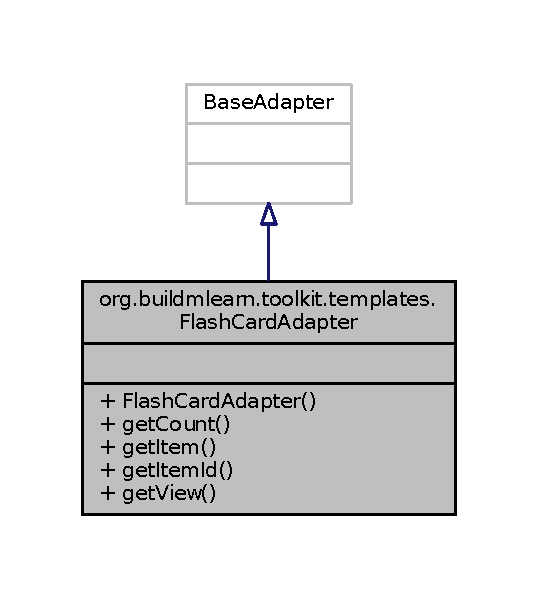
\includegraphics[width=258pt]{d5/d23/classorg_1_1buildmlearn_1_1toolkit_1_1templates_1_1FlashCardAdapter__inherit__graph}
\end{center}
\end{figure}


Collaboration diagram for org.\-buildmlearn.\-toolkit.\-templates.\-Flash\-Card\-Adapter\-:
\nopagebreak
\begin{figure}[H]
\begin{center}
\leavevmode
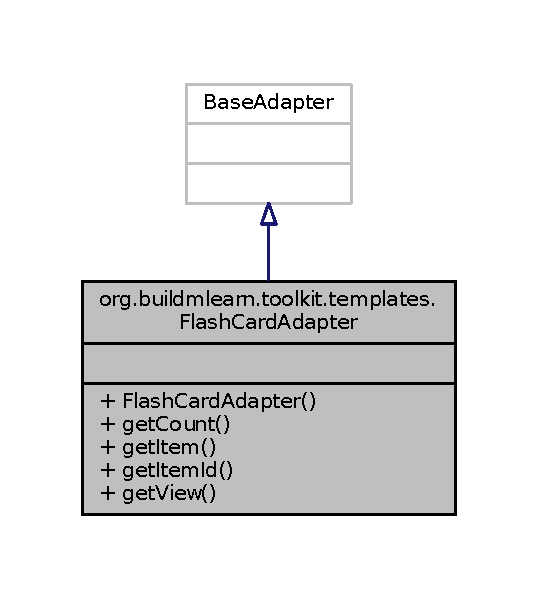
\includegraphics[width=258pt]{d0/d43/classorg_1_1buildmlearn_1_1toolkit_1_1templates_1_1FlashCardAdapter__coll__graph}
\end{center}
\end{figure}
\subsection*{Classes}
\begin{DoxyCompactItemize}
\item 
class \hyperlink{classorg_1_1buildmlearn_1_1toolkit_1_1templates_1_1FlashCardAdapter_1_1Holder}{Holder}
\end{DoxyCompactItemize}
\subsection*{Public Member Functions}
\begin{DoxyCompactItemize}
\item 
\hyperlink{classorg_1_1buildmlearn_1_1toolkit_1_1templates_1_1FlashCardAdapter_a865c27585b7f0653f0d963bf301c2303}{Flash\-Card\-Adapter} (Context context, Array\-List$<$ \hyperlink{classorg_1_1buildmlearn_1_1toolkit_1_1templates_1_1FlashCardModel}{Flash\-Card\-Model} $>$ data)
\item 
int \hyperlink{classorg_1_1buildmlearn_1_1toolkit_1_1templates_1_1FlashCardAdapter_af4d1bfcc51a9f945d4a0f0afe12adfc2}{get\-Count} ()
\item 
\hyperlink{classorg_1_1buildmlearn_1_1toolkit_1_1templates_1_1FlashCardModel}{Flash\-Card\-Model} \hyperlink{classorg_1_1buildmlearn_1_1toolkit_1_1templates_1_1FlashCardAdapter_a30e4366accf2cec71f6b642e84d610ea}{get\-Item} (int position)
\item 
long \hyperlink{classorg_1_1buildmlearn_1_1toolkit_1_1templates_1_1FlashCardAdapter_a01bdc573acbbd2ab5965df2756095bff}{get\-Item\-Id} (int position)
\item 
View \hyperlink{classorg_1_1buildmlearn_1_1toolkit_1_1templates_1_1FlashCardAdapter_ab93c5e59e63f2604b2a782b9a094179a}{get\-View} (final int position, View convert\-View, View\-Group parent)
\end{DoxyCompactItemize}


\subsection{Detailed Description}
Adapter for displaying Flash Card Template Editor data. 

Created by abhishek on 12/07/15 at 11\-:56 P\-M. 

\subsection{Constructor \& Destructor Documentation}
\hypertarget{classorg_1_1buildmlearn_1_1toolkit_1_1templates_1_1FlashCardAdapter_a865c27585b7f0653f0d963bf301c2303}{\index{org\-::buildmlearn\-::toolkit\-::templates\-::\-Flash\-Card\-Adapter@{org\-::buildmlearn\-::toolkit\-::templates\-::\-Flash\-Card\-Adapter}!Flash\-Card\-Adapter@{Flash\-Card\-Adapter}}
\index{Flash\-Card\-Adapter@{Flash\-Card\-Adapter}!org::buildmlearn::toolkit::templates::FlashCardAdapter@{org\-::buildmlearn\-::toolkit\-::templates\-::\-Flash\-Card\-Adapter}}
\subsubsection[{Flash\-Card\-Adapter}]{\setlength{\rightskip}{0pt plus 5cm}org.\-buildmlearn.\-toolkit.\-templates.\-Flash\-Card\-Adapter.\-Flash\-Card\-Adapter (
\begin{DoxyParamCaption}
\item[{Context}]{context, }
\item[{Array\-List$<$ {\bf Flash\-Card\-Model} $>$}]{data}
\end{DoxyParamCaption}
)}}\label{classorg_1_1buildmlearn_1_1toolkit_1_1templates_1_1FlashCardAdapter_a865c27585b7f0653f0d963bf301c2303}

\begin{DoxyCode}
30                                                                              \{
31         mContext = context;
32         mData = data;
33     \}
\end{DoxyCode}


\subsection{Member Function Documentation}
\hypertarget{classorg_1_1buildmlearn_1_1toolkit_1_1templates_1_1FlashCardAdapter_af4d1bfcc51a9f945d4a0f0afe12adfc2}{\index{org\-::buildmlearn\-::toolkit\-::templates\-::\-Flash\-Card\-Adapter@{org\-::buildmlearn\-::toolkit\-::templates\-::\-Flash\-Card\-Adapter}!get\-Count@{get\-Count}}
\index{get\-Count@{get\-Count}!org::buildmlearn::toolkit::templates::FlashCardAdapter@{org\-::buildmlearn\-::toolkit\-::templates\-::\-Flash\-Card\-Adapter}}
\subsubsection[{get\-Count}]{\setlength{\rightskip}{0pt plus 5cm}int org.\-buildmlearn.\-toolkit.\-templates.\-Flash\-Card\-Adapter.\-get\-Count (
\begin{DoxyParamCaption}
{}
\end{DoxyParamCaption}
)}}\label{classorg_1_1buildmlearn_1_1toolkit_1_1templates_1_1FlashCardAdapter_af4d1bfcc51a9f945d4a0f0afe12adfc2}

\begin{DoxyCode}
36                           \{
37         \textcolor{keywordflow}{return} mData.size();
38     \}
\end{DoxyCode}
\hypertarget{classorg_1_1buildmlearn_1_1toolkit_1_1templates_1_1FlashCardAdapter_a30e4366accf2cec71f6b642e84d610ea}{\index{org\-::buildmlearn\-::toolkit\-::templates\-::\-Flash\-Card\-Adapter@{org\-::buildmlearn\-::toolkit\-::templates\-::\-Flash\-Card\-Adapter}!get\-Item@{get\-Item}}
\index{get\-Item@{get\-Item}!org::buildmlearn::toolkit::templates::FlashCardAdapter@{org\-::buildmlearn\-::toolkit\-::templates\-::\-Flash\-Card\-Adapter}}
\subsubsection[{get\-Item}]{\setlength{\rightskip}{0pt plus 5cm}{\bf Flash\-Card\-Model} org.\-buildmlearn.\-toolkit.\-templates.\-Flash\-Card\-Adapter.\-get\-Item (
\begin{DoxyParamCaption}
\item[{int}]{position}
\end{DoxyParamCaption}
)}}\label{classorg_1_1buildmlearn_1_1toolkit_1_1templates_1_1FlashCardAdapter_a30e4366accf2cec71f6b642e84d610ea}

\begin{DoxyCode}
41                                                 \{
42         \textcolor{keywordflow}{return} mData.get(position);
43     \}
\end{DoxyCode}
\hypertarget{classorg_1_1buildmlearn_1_1toolkit_1_1templates_1_1FlashCardAdapter_a01bdc573acbbd2ab5965df2756095bff}{\index{org\-::buildmlearn\-::toolkit\-::templates\-::\-Flash\-Card\-Adapter@{org\-::buildmlearn\-::toolkit\-::templates\-::\-Flash\-Card\-Adapter}!get\-Item\-Id@{get\-Item\-Id}}
\index{get\-Item\-Id@{get\-Item\-Id}!org::buildmlearn::toolkit::templates::FlashCardAdapter@{org\-::buildmlearn\-::toolkit\-::templates\-::\-Flash\-Card\-Adapter}}
\subsubsection[{get\-Item\-Id}]{\setlength{\rightskip}{0pt plus 5cm}long org.\-buildmlearn.\-toolkit.\-templates.\-Flash\-Card\-Adapter.\-get\-Item\-Id (
\begin{DoxyParamCaption}
\item[{int}]{position}
\end{DoxyParamCaption}
)}}\label{classorg_1_1buildmlearn_1_1toolkit_1_1templates_1_1FlashCardAdapter_a01bdc573acbbd2ab5965df2756095bff}

\begin{DoxyCode}
46                                         \{
47 
48 
49         \textcolor{keywordflow}{return} position;
50     \}
\end{DoxyCode}
\hypertarget{classorg_1_1buildmlearn_1_1toolkit_1_1templates_1_1FlashCardAdapter_ab93c5e59e63f2604b2a782b9a094179a}{\index{org\-::buildmlearn\-::toolkit\-::templates\-::\-Flash\-Card\-Adapter@{org\-::buildmlearn\-::toolkit\-::templates\-::\-Flash\-Card\-Adapter}!get\-View@{get\-View}}
\index{get\-View@{get\-View}!org::buildmlearn::toolkit::templates::FlashCardAdapter@{org\-::buildmlearn\-::toolkit\-::templates\-::\-Flash\-Card\-Adapter}}
\subsubsection[{get\-View}]{\setlength{\rightskip}{0pt plus 5cm}View org.\-buildmlearn.\-toolkit.\-templates.\-Flash\-Card\-Adapter.\-get\-View (
\begin{DoxyParamCaption}
\item[{final int}]{position, }
\item[{View}]{convert\-View, }
\item[{View\-Group}]{parent}
\end{DoxyParamCaption}
)}}\label{classorg_1_1buildmlearn_1_1toolkit_1_1templates_1_1FlashCardAdapter_ab93c5e59e63f2604b2a782b9a094179a}

\begin{DoxyCode}
53                                                                                 \{
54 
55         LayoutInflater mInflater;
56         mInflater = LayoutInflater.from(mContext);
57         Holder holder;
58         \textcolor{keywordflow}{if} (convertView == null) \{
59             convertView = mInflater.inflate(R.layout.flash\_template\_item, parent, \textcolor{keyword}{false});
60             holder = \textcolor{keyword}{new} Holder();
61 
62             holder.question = (TextViewPlus) convertView.findViewById(R.id.flash\_item\_question);
63             holder.answer = (TextViewPlus) convertView.findViewById(R.id.flash\_item\_answer);
64             holder.hint = (TextViewPlus) convertView.findViewById(R.id.flash\_item\_hint);
65             holder.image = (ImageView) convertView.findViewById(R.id.flash\_item\_image);
66 
67             holder.delete = (ImageView) convertView.findViewById(R.id.flash\_template\_delete);
68             holder.edit = (ImageView) convertView.findViewById(R.id.flash\_item\_edit);
69 
70         \} \textcolor{keywordflow}{else} \{
71             holder = (Holder) convertView.getTag();
72         \}
73 
74         \textcolor{keyword}{final} FlashCardModel data = \hyperlink{classorg_1_1buildmlearn_1_1toolkit_1_1templates_1_1FlashCardAdapter_a30e4366accf2cec71f6b642e84d610ea}{getItem}(position);
75         holder.answer.setText(data.getAnswer());
76         holder.image.setImageBitmap(data.getImageBitmap());
77         holder.hint.setText(data.getHint());
78         holder.question.setText(data.getQuestion());
79 
80         holder.edit.setOnClickListener(\textcolor{keyword}{new} View.OnClickListener() \{
81             @Override
82             \textcolor{keyword}{public} \textcolor{keywordtype}{void} onClick(View v) \{
83                 Toast.makeText(mContext, \textcolor{stringliteral}{"Long press to edit this item"}, Toast.LENGTH\_SHORT).show();
84             \}
85         \});
86 
87         holder.delete.setOnClickListener(\textcolor{keyword}{new} View.OnClickListener() \{
88             @Override
89             \textcolor{keyword}{public} \textcolor{keywordtype}{void} onClick(View v) \{
90 
91                 \textcolor{keyword}{final} MaterialDialog dialog = \textcolor{keyword}{new} MaterialDialog.Builder(mContext)
92                         .title(R.string.info\_template\_delete)
93                         .content(R.string.info\_delete\_item\_content)
94                         .positiveText(R.string.dialog\_yes)
95                         .negativeText(R.string.dialog\_no)
96                         .build();
97 
98                 dialog.getActionButton(DialogAction.POSITIVE).setOnClickListener(\textcolor{keyword}{new} View.OnClickListener()
       \{
99                     @Override
100                     \textcolor{keyword}{public} \textcolor{keywordtype}{void} onClick(View v) \{
101                         mData.remove(position);
102                         notifyDataSetChanged();
103                         dialog.dismiss();
104                     \}
105                 \});
106 
107                 dialog.show();
108 
109             \}
110         \});
111 
112 
113         convertView.setTag(holder);
114 
115         \textcolor{keywordflow}{return} convertView;
116     \}
\end{DoxyCode}


The documentation for this class was generated from the following file\-:\begin{DoxyCompactItemize}
\item 
/\-Buildm\-Learn-\/\-Toolkit-\/\-Android/source-\/code/app/src/main/java/org/buildmlearn/toolkit/templates/\hyperlink{FlashCardAdapter_8java}{Flash\-Card\-Adapter.\-java}\end{DoxyCompactItemize}

\hypertarget{classorg_1_1buildmlearn_1_1toolkit_1_1templates_1_1FlashCardModel}{\section{org.\-buildmlearn.\-toolkit.\-templates.\-Flash\-Card\-Model Class Reference}
\label{classorg_1_1buildmlearn_1_1toolkit_1_1templates_1_1FlashCardModel}\index{org.\-buildmlearn.\-toolkit.\-templates.\-Flash\-Card\-Model@{org.\-buildmlearn.\-toolkit.\-templates.\-Flash\-Card\-Model}}
}


Model class for Flash Card Template Editor data.  




Inheritance diagram for org.\-buildmlearn.\-toolkit.\-templates.\-Flash\-Card\-Model\-:
\nopagebreak
\begin{figure}[H]
\begin{center}
\leavevmode
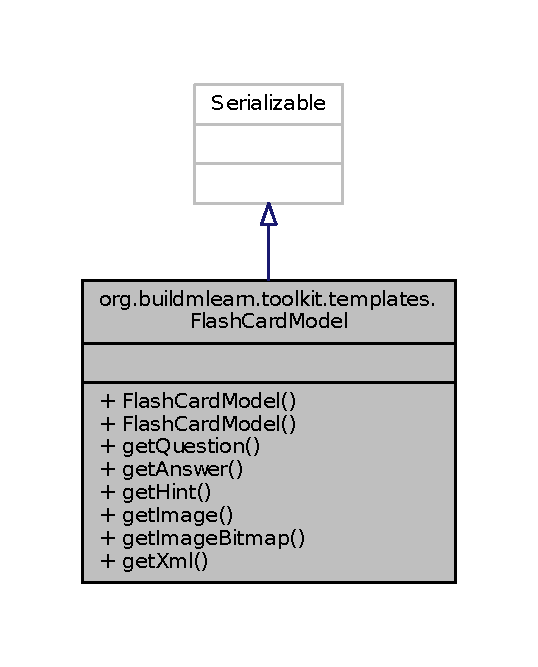
\includegraphics[width=258pt]{df/d5d/classorg_1_1buildmlearn_1_1toolkit_1_1templates_1_1FlashCardModel__inherit__graph}
\end{center}
\end{figure}


Collaboration diagram for org.\-buildmlearn.\-toolkit.\-templates.\-Flash\-Card\-Model\-:
\nopagebreak
\begin{figure}[H]
\begin{center}
\leavevmode
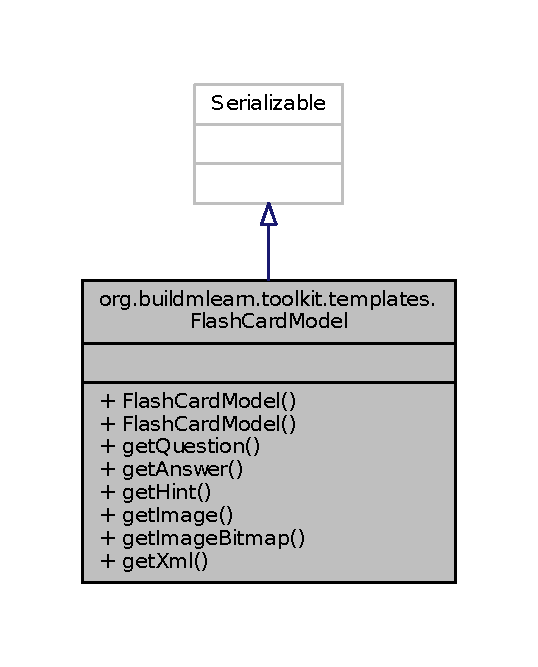
\includegraphics[width=258pt]{d6/da7/classorg_1_1buildmlearn_1_1toolkit_1_1templates_1_1FlashCardModel__coll__graph}
\end{center}
\end{figure}
\subsection*{Public Member Functions}
\begin{DoxyCompactItemize}
\item 
\hyperlink{classorg_1_1buildmlearn_1_1toolkit_1_1templates_1_1FlashCardModel_a2dd9b2a68f1b2b6ada40d09b5a641f64}{Flash\-Card\-Model} (String question, String answer, String hint, Bitmap image)
\item 
\hyperlink{classorg_1_1buildmlearn_1_1toolkit_1_1templates_1_1FlashCardModel_ab57e165bc61b3bc72c50a7fbadabedbe}{Flash\-Card\-Model} (String question, String answer, String hint, String image)
\item 
String \hyperlink{classorg_1_1buildmlearn_1_1toolkit_1_1templates_1_1FlashCardModel_abf8ce19f627a4783f734dd05366c83be}{get\-Question} ()
\item 
String \hyperlink{classorg_1_1buildmlearn_1_1toolkit_1_1templates_1_1FlashCardModel_af7ada5f29f1967ffe976b8c1ac513c5e}{get\-Answer} ()
\item 
String \hyperlink{classorg_1_1buildmlearn_1_1toolkit_1_1templates_1_1FlashCardModel_a89685e7a56be83bd6718ba0b3eb88eb0}{get\-Hint} ()
\item 
String \hyperlink{classorg_1_1buildmlearn_1_1toolkit_1_1templates_1_1FlashCardModel_a80528eb28bb619a07090f7766f2de410}{get\-Image} ()
\item 
Bitmap \hyperlink{classorg_1_1buildmlearn_1_1toolkit_1_1templates_1_1FlashCardModel_acc164af071d93c3ab9348310f3dbf8aa}{get\-Image\-Bitmap} ()
\item 
Element \hyperlink{classorg_1_1buildmlearn_1_1toolkit_1_1templates_1_1FlashCardModel_a08112a6fbb90f87602d2b96da37e8cd8}{get\-Xml} (Document doc)
\end{DoxyCompactItemize}


\subsection{Detailed Description}
Model class for Flash Card Template Editor data. 

Created by abhishek on 11/07/15 at 7\-:34 P\-M. 

\subsection{Constructor \& Destructor Documentation}
\hypertarget{classorg_1_1buildmlearn_1_1toolkit_1_1templates_1_1FlashCardModel_a2dd9b2a68f1b2b6ada40d09b5a641f64}{\index{org\-::buildmlearn\-::toolkit\-::templates\-::\-Flash\-Card\-Model@{org\-::buildmlearn\-::toolkit\-::templates\-::\-Flash\-Card\-Model}!Flash\-Card\-Model@{Flash\-Card\-Model}}
\index{Flash\-Card\-Model@{Flash\-Card\-Model}!org::buildmlearn::toolkit::templates::FlashCardModel@{org\-::buildmlearn\-::toolkit\-::templates\-::\-Flash\-Card\-Model}}
\subsubsection[{Flash\-Card\-Model}]{\setlength{\rightskip}{0pt plus 5cm}org.\-buildmlearn.\-toolkit.\-templates.\-Flash\-Card\-Model.\-Flash\-Card\-Model (
\begin{DoxyParamCaption}
\item[{String}]{question, }
\item[{String}]{answer, }
\item[{String}]{hint, }
\item[{Bitmap}]{image}
\end{DoxyParamCaption}
)}}\label{classorg_1_1buildmlearn_1_1toolkit_1_1templates_1_1FlashCardModel_a2dd9b2a68f1b2b6ada40d09b5a641f64}

\begin{DoxyCode}
25                                                                                      \{
26         mQuestion = question;
27         mAnswer = answer;
28         mHint = hint;
29         mImage = convertBitmapToBase64(image);
30     \}
\end{DoxyCode}
\hypertarget{classorg_1_1buildmlearn_1_1toolkit_1_1templates_1_1FlashCardModel_ab57e165bc61b3bc72c50a7fbadabedbe}{\index{org\-::buildmlearn\-::toolkit\-::templates\-::\-Flash\-Card\-Model@{org\-::buildmlearn\-::toolkit\-::templates\-::\-Flash\-Card\-Model}!Flash\-Card\-Model@{Flash\-Card\-Model}}
\index{Flash\-Card\-Model@{Flash\-Card\-Model}!org::buildmlearn::toolkit::templates::FlashCardModel@{org\-::buildmlearn\-::toolkit\-::templates\-::\-Flash\-Card\-Model}}
\subsubsection[{Flash\-Card\-Model}]{\setlength{\rightskip}{0pt plus 5cm}org.\-buildmlearn.\-toolkit.\-templates.\-Flash\-Card\-Model.\-Flash\-Card\-Model (
\begin{DoxyParamCaption}
\item[{String}]{question, }
\item[{String}]{answer, }
\item[{String}]{hint, }
\item[{String}]{image}
\end{DoxyParamCaption}
)}}\label{classorg_1_1buildmlearn_1_1toolkit_1_1templates_1_1FlashCardModel_ab57e165bc61b3bc72c50a7fbadabedbe}

\begin{DoxyCode}
32                                                                                      \{
33         mQuestion = question;
34         mAnswer = answer;
35         mHint = hint;
36         mImage = image;
37     \}
\end{DoxyCode}


\subsection{Member Function Documentation}
\hypertarget{classorg_1_1buildmlearn_1_1toolkit_1_1templates_1_1FlashCardModel_af7ada5f29f1967ffe976b8c1ac513c5e}{\index{org\-::buildmlearn\-::toolkit\-::templates\-::\-Flash\-Card\-Model@{org\-::buildmlearn\-::toolkit\-::templates\-::\-Flash\-Card\-Model}!get\-Answer@{get\-Answer}}
\index{get\-Answer@{get\-Answer}!org::buildmlearn::toolkit::templates::FlashCardModel@{org\-::buildmlearn\-::toolkit\-::templates\-::\-Flash\-Card\-Model}}
\subsubsection[{get\-Answer}]{\setlength{\rightskip}{0pt plus 5cm}String org.\-buildmlearn.\-toolkit.\-templates.\-Flash\-Card\-Model.\-get\-Answer (
\begin{DoxyParamCaption}
{}
\end{DoxyParamCaption}
)}}\label{classorg_1_1buildmlearn_1_1toolkit_1_1templates_1_1FlashCardModel_af7ada5f29f1967ffe976b8c1ac513c5e}

\begin{DoxyCode}
54                               \{
55         \textcolor{keywordflow}{return} mAnswer;
56     \}
\end{DoxyCode}
\hypertarget{classorg_1_1buildmlearn_1_1toolkit_1_1templates_1_1FlashCardModel_a89685e7a56be83bd6718ba0b3eb88eb0}{\index{org\-::buildmlearn\-::toolkit\-::templates\-::\-Flash\-Card\-Model@{org\-::buildmlearn\-::toolkit\-::templates\-::\-Flash\-Card\-Model}!get\-Hint@{get\-Hint}}
\index{get\-Hint@{get\-Hint}!org::buildmlearn::toolkit::templates::FlashCardModel@{org\-::buildmlearn\-::toolkit\-::templates\-::\-Flash\-Card\-Model}}
\subsubsection[{get\-Hint}]{\setlength{\rightskip}{0pt plus 5cm}String org.\-buildmlearn.\-toolkit.\-templates.\-Flash\-Card\-Model.\-get\-Hint (
\begin{DoxyParamCaption}
{}
\end{DoxyParamCaption}
)}}\label{classorg_1_1buildmlearn_1_1toolkit_1_1templates_1_1FlashCardModel_a89685e7a56be83bd6718ba0b3eb88eb0}

\begin{DoxyCode}
58                             \{
59         \textcolor{keywordflow}{return} mHint;
60     \}
\end{DoxyCode}
\hypertarget{classorg_1_1buildmlearn_1_1toolkit_1_1templates_1_1FlashCardModel_a80528eb28bb619a07090f7766f2de410}{\index{org\-::buildmlearn\-::toolkit\-::templates\-::\-Flash\-Card\-Model@{org\-::buildmlearn\-::toolkit\-::templates\-::\-Flash\-Card\-Model}!get\-Image@{get\-Image}}
\index{get\-Image@{get\-Image}!org::buildmlearn::toolkit::templates::FlashCardModel@{org\-::buildmlearn\-::toolkit\-::templates\-::\-Flash\-Card\-Model}}
\subsubsection[{get\-Image}]{\setlength{\rightskip}{0pt plus 5cm}String org.\-buildmlearn.\-toolkit.\-templates.\-Flash\-Card\-Model.\-get\-Image (
\begin{DoxyParamCaption}
{}
\end{DoxyParamCaption}
)}}\label{classorg_1_1buildmlearn_1_1toolkit_1_1templates_1_1FlashCardModel_a80528eb28bb619a07090f7766f2de410}

\begin{DoxyCode}
62                              \{
63         \textcolor{keywordflow}{return} mImage;
64     \}
\end{DoxyCode}
\hypertarget{classorg_1_1buildmlearn_1_1toolkit_1_1templates_1_1FlashCardModel_acc164af071d93c3ab9348310f3dbf8aa}{\index{org\-::buildmlearn\-::toolkit\-::templates\-::\-Flash\-Card\-Model@{org\-::buildmlearn\-::toolkit\-::templates\-::\-Flash\-Card\-Model}!get\-Image\-Bitmap@{get\-Image\-Bitmap}}
\index{get\-Image\-Bitmap@{get\-Image\-Bitmap}!org::buildmlearn::toolkit::templates::FlashCardModel@{org\-::buildmlearn\-::toolkit\-::templates\-::\-Flash\-Card\-Model}}
\subsubsection[{get\-Image\-Bitmap}]{\setlength{\rightskip}{0pt plus 5cm}Bitmap org.\-buildmlearn.\-toolkit.\-templates.\-Flash\-Card\-Model.\-get\-Image\-Bitmap (
\begin{DoxyParamCaption}
{}
\end{DoxyParamCaption}
)}}\label{classorg_1_1buildmlearn_1_1toolkit_1_1templates_1_1FlashCardModel_acc164af071d93c3ab9348310f3dbf8aa}

\begin{DoxyCode}
66                                    \{
67         byte[] decodedString = Base64.decode(mImage, Base64.DEFAULT);
68         Bitmap decodedByte = BitmapFactory.decodeByteArray(decodedString, 0, decodedString.length);
69         \textcolor{keywordflow}{return} decodedByte;
70     \}
\end{DoxyCode}
\hypertarget{classorg_1_1buildmlearn_1_1toolkit_1_1templates_1_1FlashCardModel_abf8ce19f627a4783f734dd05366c83be}{\index{org\-::buildmlearn\-::toolkit\-::templates\-::\-Flash\-Card\-Model@{org\-::buildmlearn\-::toolkit\-::templates\-::\-Flash\-Card\-Model}!get\-Question@{get\-Question}}
\index{get\-Question@{get\-Question}!org::buildmlearn::toolkit::templates::FlashCardModel@{org\-::buildmlearn\-::toolkit\-::templates\-::\-Flash\-Card\-Model}}
\subsubsection[{get\-Question}]{\setlength{\rightskip}{0pt plus 5cm}String org.\-buildmlearn.\-toolkit.\-templates.\-Flash\-Card\-Model.\-get\-Question (
\begin{DoxyParamCaption}
{}
\end{DoxyParamCaption}
)}}\label{classorg_1_1buildmlearn_1_1toolkit_1_1templates_1_1FlashCardModel_abf8ce19f627a4783f734dd05366c83be}

\begin{DoxyCode}
50                                 \{
51         \textcolor{keywordflow}{return} mQuestion;
52     \}
\end{DoxyCode}
\hypertarget{classorg_1_1buildmlearn_1_1toolkit_1_1templates_1_1FlashCardModel_a08112a6fbb90f87602d2b96da37e8cd8}{\index{org\-::buildmlearn\-::toolkit\-::templates\-::\-Flash\-Card\-Model@{org\-::buildmlearn\-::toolkit\-::templates\-::\-Flash\-Card\-Model}!get\-Xml@{get\-Xml}}
\index{get\-Xml@{get\-Xml}!org::buildmlearn::toolkit::templates::FlashCardModel@{org\-::buildmlearn\-::toolkit\-::templates\-::\-Flash\-Card\-Model}}
\subsubsection[{get\-Xml}]{\setlength{\rightskip}{0pt plus 5cm}Element org.\-buildmlearn.\-toolkit.\-templates.\-Flash\-Card\-Model.\-get\-Xml (
\begin{DoxyParamCaption}
\item[{Document}]{doc}
\end{DoxyParamCaption}
)}}\label{classorg_1_1buildmlearn_1_1toolkit_1_1templates_1_1FlashCardModel_a08112a6fbb90f87602d2b96da37e8cd8}

\begin{DoxyCode}
72                                         \{
73         Element rootElement = doc.createElement(\textcolor{stringliteral}{"item"});
74         Element questionElement = doc.createElement(\textcolor{stringliteral}{"question"});
75         questionElement.appendChild(doc.createTextNode(mQuestion));
76         rootElement.appendChild(questionElement);
77 
78         Element answerElement = doc.createElement(\textcolor{stringliteral}{"answer"});
79         answerElement.appendChild(doc.createTextNode(String.valueOf(mAnswer)));
80         rootElement.appendChild(answerElement);
81 
82         Element hintElement = doc.createElement(\textcolor{stringliteral}{"hint"});
83         hintElement.appendChild(doc.createTextNode(String.valueOf(mHint)));
84         rootElement.appendChild(hintElement);
85 
86         Element imageElement = doc.createElement(\textcolor{stringliteral}{"image"});
87         imageElement.appendChild(doc.createTextNode(String.valueOf(mImage)));
88         rootElement.appendChild(imageElement);
89         \textcolor{keywordflow}{return} rootElement;
90     \}
\end{DoxyCode}


The documentation for this class was generated from the following file\-:\begin{DoxyCompactItemize}
\item 
/\-Buildm\-Learn-\/\-Toolkit-\/\-Android/source-\/code/app/src/main/java/org/buildmlearn/toolkit/templates/\hyperlink{FlashCardModel_8java}{Flash\-Card\-Model.\-java}\end{DoxyCompactItemize}

\hypertarget{classorg_1_1buildmlearn_1_1toolkit_1_1flashcardtemplate_1_1FlashModel}{\section{org.\-buildmlearn.\-toolkit.\-flashcardtemplate.\-Flash\-Model Class Reference}
\label{classorg_1_1buildmlearn_1_1toolkit_1_1flashcardtemplate_1_1FlashModel}\index{org.\-buildmlearn.\-toolkit.\-flashcardtemplate.\-Flash\-Model@{org.\-buildmlearn.\-toolkit.\-flashcardtemplate.\-Flash\-Model}}
}


Simulator code for Flash Card Template.  




Collaboration diagram for org.\-buildmlearn.\-toolkit.\-flashcardtemplate.\-Flash\-Model\-:
\nopagebreak
\begin{figure}[H]
\begin{center}
\leavevmode
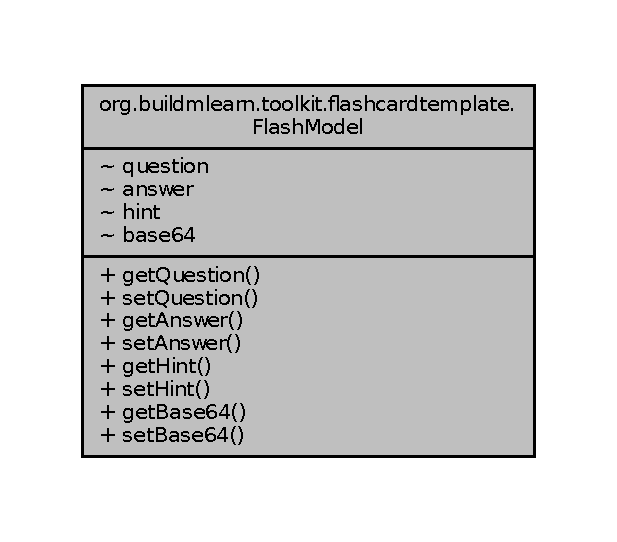
\includegraphics[width=296pt]{d1/d4f/classorg_1_1buildmlearn_1_1toolkit_1_1flashcardtemplate_1_1FlashModel__coll__graph}
\end{center}
\end{figure}
\subsection*{Public Member Functions}
\begin{DoxyCompactItemize}
\item 
String \hyperlink{classorg_1_1buildmlearn_1_1toolkit_1_1flashcardtemplate_1_1FlashModel_a744ea87d54ba5157cdbcb1040e69513b}{get\-Question} ()
\item 
void \hyperlink{classorg_1_1buildmlearn_1_1toolkit_1_1flashcardtemplate_1_1FlashModel_a56b3cc8d0409716e1a9fc55da494b599}{set\-Question} (String question)
\item 
String \hyperlink{classorg_1_1buildmlearn_1_1toolkit_1_1flashcardtemplate_1_1FlashModel_a00d25c8fec3369101a07d40f4864f9ec}{get\-Answer} ()
\item 
void \hyperlink{classorg_1_1buildmlearn_1_1toolkit_1_1flashcardtemplate_1_1FlashModel_adcaaa02610df25395e0f3e8b3c2dbf9f}{set\-Answer} (String answer)
\item 
String \hyperlink{classorg_1_1buildmlearn_1_1toolkit_1_1flashcardtemplate_1_1FlashModel_a34763f0c06917ebe3935536c1bbc0892}{get\-Hint} ()
\item 
void \hyperlink{classorg_1_1buildmlearn_1_1toolkit_1_1flashcardtemplate_1_1FlashModel_a3e73de81abaa849ff6495f755cc71f4f}{set\-Hint} (String hint)
\item 
String \hyperlink{classorg_1_1buildmlearn_1_1toolkit_1_1flashcardtemplate_1_1FlashModel_a19f35d4b212678b8b75a33b3a7331f87}{get\-Base64} ()
\item 
void \hyperlink{classorg_1_1buildmlearn_1_1toolkit_1_1flashcardtemplate_1_1FlashModel_a421a4fae8a53309901249e6b16d3bab2}{set\-Base64} (String base64)
\end{DoxyCompactItemize}


\subsection{Detailed Description}
Simulator code for Flash Card Template. 

\subsection{Member Function Documentation}
\hypertarget{classorg_1_1buildmlearn_1_1toolkit_1_1flashcardtemplate_1_1FlashModel_a00d25c8fec3369101a07d40f4864f9ec}{\index{org\-::buildmlearn\-::toolkit\-::flashcardtemplate\-::\-Flash\-Model@{org\-::buildmlearn\-::toolkit\-::flashcardtemplate\-::\-Flash\-Model}!get\-Answer@{get\-Answer}}
\index{get\-Answer@{get\-Answer}!org::buildmlearn::toolkit::flashcardtemplate::FlashModel@{org\-::buildmlearn\-::toolkit\-::flashcardtemplate\-::\-Flash\-Model}}
\subsubsection[{get\-Answer}]{\setlength{\rightskip}{0pt plus 5cm}String org.\-buildmlearn.\-toolkit.\-flashcardtemplate.\-Flash\-Model.\-get\-Answer (
\begin{DoxyParamCaption}
{}
\end{DoxyParamCaption}
)}}\label{classorg_1_1buildmlearn_1_1toolkit_1_1flashcardtemplate_1_1FlashModel_a00d25c8fec3369101a07d40f4864f9ec}

\begin{DoxyCode}
19                               \{
20         \textcolor{keywordflow}{return} answer;
21     \}
\end{DoxyCode}
\hypertarget{classorg_1_1buildmlearn_1_1toolkit_1_1flashcardtemplate_1_1FlashModel_a19f35d4b212678b8b75a33b3a7331f87}{\index{org\-::buildmlearn\-::toolkit\-::flashcardtemplate\-::\-Flash\-Model@{org\-::buildmlearn\-::toolkit\-::flashcardtemplate\-::\-Flash\-Model}!get\-Base64@{get\-Base64}}
\index{get\-Base64@{get\-Base64}!org::buildmlearn::toolkit::flashcardtemplate::FlashModel@{org\-::buildmlearn\-::toolkit\-::flashcardtemplate\-::\-Flash\-Model}}
\subsubsection[{get\-Base64}]{\setlength{\rightskip}{0pt plus 5cm}String org.\-buildmlearn.\-toolkit.\-flashcardtemplate.\-Flash\-Model.\-get\-Base64 (
\begin{DoxyParamCaption}
{}
\end{DoxyParamCaption}
)}}\label{classorg_1_1buildmlearn_1_1toolkit_1_1flashcardtemplate_1_1FlashModel_a19f35d4b212678b8b75a33b3a7331f87}

\begin{DoxyCode}
35                               \{
36         \textcolor{keywordflow}{return} base64;
37     \}
\end{DoxyCode}
\hypertarget{classorg_1_1buildmlearn_1_1toolkit_1_1flashcardtemplate_1_1FlashModel_a34763f0c06917ebe3935536c1bbc0892}{\index{org\-::buildmlearn\-::toolkit\-::flashcardtemplate\-::\-Flash\-Model@{org\-::buildmlearn\-::toolkit\-::flashcardtemplate\-::\-Flash\-Model}!get\-Hint@{get\-Hint}}
\index{get\-Hint@{get\-Hint}!org::buildmlearn::toolkit::flashcardtemplate::FlashModel@{org\-::buildmlearn\-::toolkit\-::flashcardtemplate\-::\-Flash\-Model}}
\subsubsection[{get\-Hint}]{\setlength{\rightskip}{0pt plus 5cm}String org.\-buildmlearn.\-toolkit.\-flashcardtemplate.\-Flash\-Model.\-get\-Hint (
\begin{DoxyParamCaption}
{}
\end{DoxyParamCaption}
)}}\label{classorg_1_1buildmlearn_1_1toolkit_1_1flashcardtemplate_1_1FlashModel_a34763f0c06917ebe3935536c1bbc0892}

\begin{DoxyCode}
27                             \{
28         \textcolor{keywordflow}{return} hint;
29     \}
\end{DoxyCode}
\hypertarget{classorg_1_1buildmlearn_1_1toolkit_1_1flashcardtemplate_1_1FlashModel_a744ea87d54ba5157cdbcb1040e69513b}{\index{org\-::buildmlearn\-::toolkit\-::flashcardtemplate\-::\-Flash\-Model@{org\-::buildmlearn\-::toolkit\-::flashcardtemplate\-::\-Flash\-Model}!get\-Question@{get\-Question}}
\index{get\-Question@{get\-Question}!org::buildmlearn::toolkit::flashcardtemplate::FlashModel@{org\-::buildmlearn\-::toolkit\-::flashcardtemplate\-::\-Flash\-Model}}
\subsubsection[{get\-Question}]{\setlength{\rightskip}{0pt plus 5cm}String org.\-buildmlearn.\-toolkit.\-flashcardtemplate.\-Flash\-Model.\-get\-Question (
\begin{DoxyParamCaption}
{}
\end{DoxyParamCaption}
)}}\label{classorg_1_1buildmlearn_1_1toolkit_1_1flashcardtemplate_1_1FlashModel_a744ea87d54ba5157cdbcb1040e69513b}

\begin{DoxyCode}
11                                 \{
12         \textcolor{keywordflow}{return} question;
13     \}
\end{DoxyCode}
\hypertarget{classorg_1_1buildmlearn_1_1toolkit_1_1flashcardtemplate_1_1FlashModel_adcaaa02610df25395e0f3e8b3c2dbf9f}{\index{org\-::buildmlearn\-::toolkit\-::flashcardtemplate\-::\-Flash\-Model@{org\-::buildmlearn\-::toolkit\-::flashcardtemplate\-::\-Flash\-Model}!set\-Answer@{set\-Answer}}
\index{set\-Answer@{set\-Answer}!org::buildmlearn::toolkit::flashcardtemplate::FlashModel@{org\-::buildmlearn\-::toolkit\-::flashcardtemplate\-::\-Flash\-Model}}
\subsubsection[{set\-Answer}]{\setlength{\rightskip}{0pt plus 5cm}void org.\-buildmlearn.\-toolkit.\-flashcardtemplate.\-Flash\-Model.\-set\-Answer (
\begin{DoxyParamCaption}
\item[{String}]{answer}
\end{DoxyParamCaption}
)}}\label{classorg_1_1buildmlearn_1_1toolkit_1_1flashcardtemplate_1_1FlashModel_adcaaa02610df25395e0f3e8b3c2dbf9f}

\begin{DoxyCode}
23                                          \{
24         this.answer = answer;
25     \}
\end{DoxyCode}
\hypertarget{classorg_1_1buildmlearn_1_1toolkit_1_1flashcardtemplate_1_1FlashModel_a421a4fae8a53309901249e6b16d3bab2}{\index{org\-::buildmlearn\-::toolkit\-::flashcardtemplate\-::\-Flash\-Model@{org\-::buildmlearn\-::toolkit\-::flashcardtemplate\-::\-Flash\-Model}!set\-Base64@{set\-Base64}}
\index{set\-Base64@{set\-Base64}!org::buildmlearn::toolkit::flashcardtemplate::FlashModel@{org\-::buildmlearn\-::toolkit\-::flashcardtemplate\-::\-Flash\-Model}}
\subsubsection[{set\-Base64}]{\setlength{\rightskip}{0pt plus 5cm}void org.\-buildmlearn.\-toolkit.\-flashcardtemplate.\-Flash\-Model.\-set\-Base64 (
\begin{DoxyParamCaption}
\item[{String}]{base64}
\end{DoxyParamCaption}
)}}\label{classorg_1_1buildmlearn_1_1toolkit_1_1flashcardtemplate_1_1FlashModel_a421a4fae8a53309901249e6b16d3bab2}

\begin{DoxyCode}
39                                          \{
40         this.base64 = base64;
41     \}
\end{DoxyCode}
\hypertarget{classorg_1_1buildmlearn_1_1toolkit_1_1flashcardtemplate_1_1FlashModel_a3e73de81abaa849ff6495f755cc71f4f}{\index{org\-::buildmlearn\-::toolkit\-::flashcardtemplate\-::\-Flash\-Model@{org\-::buildmlearn\-::toolkit\-::flashcardtemplate\-::\-Flash\-Model}!set\-Hint@{set\-Hint}}
\index{set\-Hint@{set\-Hint}!org::buildmlearn::toolkit::flashcardtemplate::FlashModel@{org\-::buildmlearn\-::toolkit\-::flashcardtemplate\-::\-Flash\-Model}}
\subsubsection[{set\-Hint}]{\setlength{\rightskip}{0pt plus 5cm}void org.\-buildmlearn.\-toolkit.\-flashcardtemplate.\-Flash\-Model.\-set\-Hint (
\begin{DoxyParamCaption}
\item[{String}]{hint}
\end{DoxyParamCaption}
)}}\label{classorg_1_1buildmlearn_1_1toolkit_1_1flashcardtemplate_1_1FlashModel_a3e73de81abaa849ff6495f755cc71f4f}

\begin{DoxyCode}
31                                      \{
32         this.hint = hint;
33     \}
\end{DoxyCode}
\hypertarget{classorg_1_1buildmlearn_1_1toolkit_1_1flashcardtemplate_1_1FlashModel_a56b3cc8d0409716e1a9fc55da494b599}{\index{org\-::buildmlearn\-::toolkit\-::flashcardtemplate\-::\-Flash\-Model@{org\-::buildmlearn\-::toolkit\-::flashcardtemplate\-::\-Flash\-Model}!set\-Question@{set\-Question}}
\index{set\-Question@{set\-Question}!org::buildmlearn::toolkit::flashcardtemplate::FlashModel@{org\-::buildmlearn\-::toolkit\-::flashcardtemplate\-::\-Flash\-Model}}
\subsubsection[{set\-Question}]{\setlength{\rightskip}{0pt plus 5cm}void org.\-buildmlearn.\-toolkit.\-flashcardtemplate.\-Flash\-Model.\-set\-Question (
\begin{DoxyParamCaption}
\item[{String}]{question}
\end{DoxyParamCaption}
)}}\label{classorg_1_1buildmlearn_1_1toolkit_1_1flashcardtemplate_1_1FlashModel_a56b3cc8d0409716e1a9fc55da494b599}

\begin{DoxyCode}
15                                              \{
16         this.question = question;
17     \}
\end{DoxyCode}


The documentation for this class was generated from the following file\-:\begin{DoxyCompactItemize}
\item 
/\-Buildm\-Learn-\/\-Toolkit-\/\-Android/source-\/code/app/src/main/java/org/buildmlearn/toolkit/flashcardtemplate/\hyperlink{FlashModel_8java}{Flash\-Model.\-java}\end{DoxyCompactItemize}

\hypertarget{classorg_1_1buildmlearn_1_1toolkit_1_1templates_1_1FlashTemplate}{\section{org.\-buildmlearn.\-toolkit.\-templates.\-Flash\-Template Class Reference}
\label{classorg_1_1buildmlearn_1_1toolkit_1_1templates_1_1FlashTemplate}\index{org.\-buildmlearn.\-toolkit.\-templates.\-Flash\-Template@{org.\-buildmlearn.\-toolkit.\-templates.\-Flash\-Template}}
}


Flash Card template code implementing methods of Template\-Interface.  




Inheritance diagram for org.\-buildmlearn.\-toolkit.\-templates.\-Flash\-Template\-:
\nopagebreak
\begin{figure}[H]
\begin{center}
\leavevmode
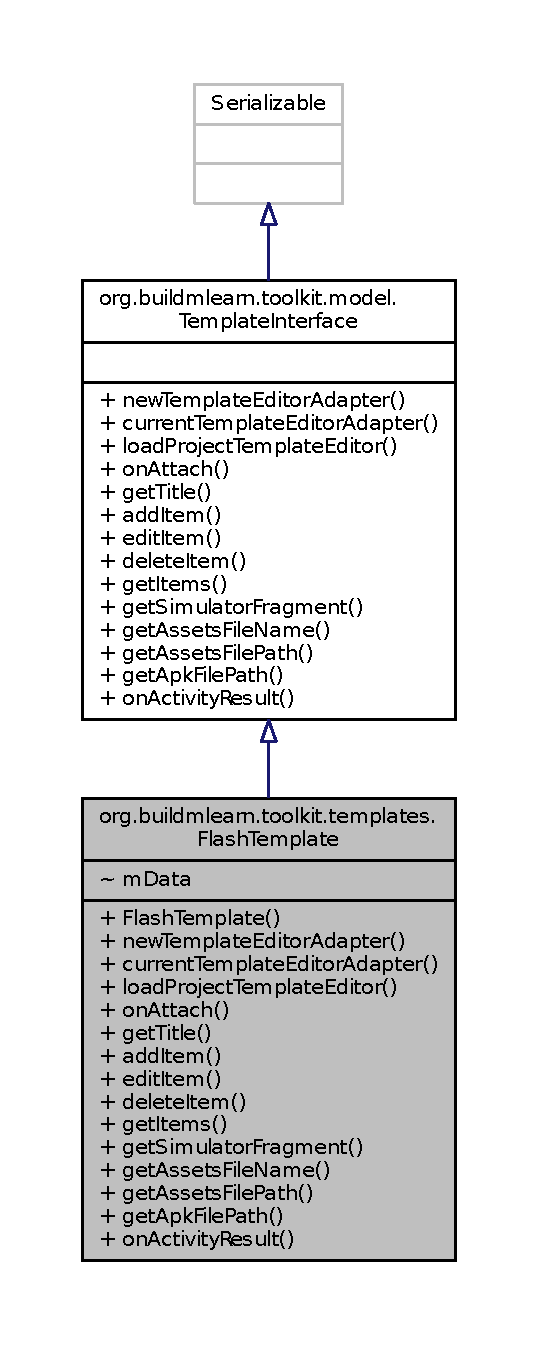
\includegraphics[height=550pt]{d4/de9/classorg_1_1buildmlearn_1_1toolkit_1_1templates_1_1FlashTemplate__inherit__graph}
\end{center}
\end{figure}


Collaboration diagram for org.\-buildmlearn.\-toolkit.\-templates.\-Flash\-Template\-:
\nopagebreak
\begin{figure}[H]
\begin{center}
\leavevmode
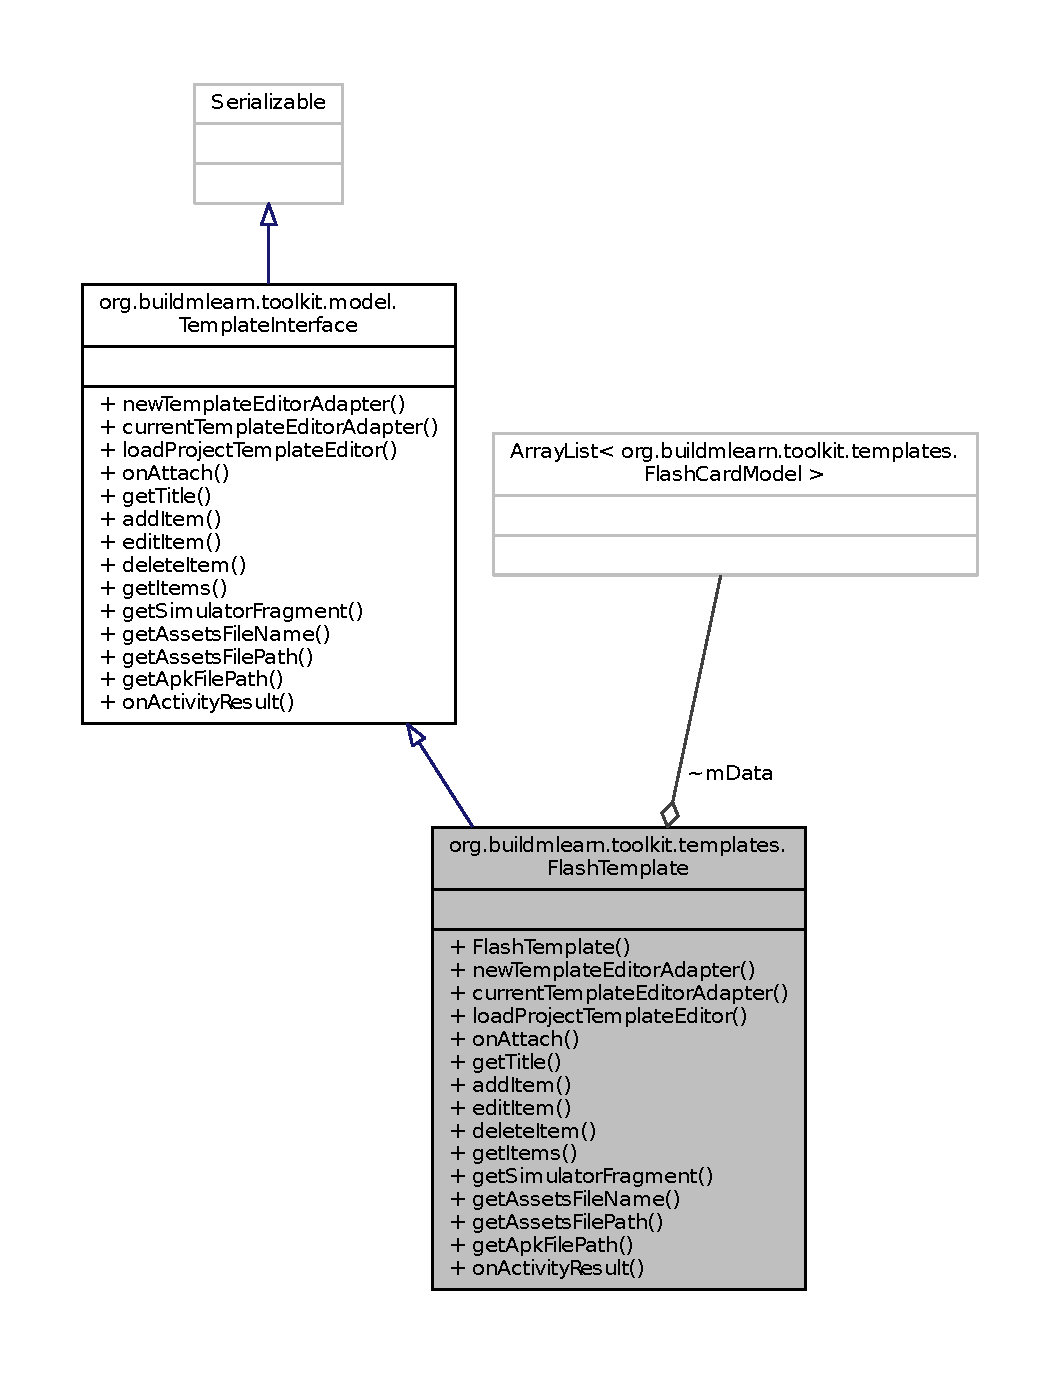
\includegraphics[width=350pt]{d9/d0b/classorg_1_1buildmlearn_1_1toolkit_1_1templates_1_1FlashTemplate__coll__graph}
\end{center}
\end{figure}
\subsection*{Public Member Functions}
\begin{DoxyCompactItemize}
\item 
\hyperlink{classorg_1_1buildmlearn_1_1toolkit_1_1templates_1_1FlashTemplate_a93eca3908cf039e1fa37e0408d0f4837}{Flash\-Template} ()
\item 
Base\-Adapter \hyperlink{classorg_1_1buildmlearn_1_1toolkit_1_1templates_1_1FlashTemplate_ad524e69199d8435959cf348558039b2d}{new\-Template\-Editor\-Adapter} (Context context)
\begin{DoxyCompactList}\small\item\em Called from Template Editor when template editor is started for creating a new template project. \end{DoxyCompactList}\item 
Base\-Adapter \hyperlink{classorg_1_1buildmlearn_1_1toolkit_1_1templates_1_1FlashTemplate_a70db96b6e7ec5e339fe106fc15d64860}{current\-Template\-Editor\-Adapter} ()
\begin{DoxyCompactList}\small\item\em This function is used to get the adapter (containing template data) for a existing/current template project. \end{DoxyCompactList}\item 
Base\-Adapter \hyperlink{classorg_1_1buildmlearn_1_1toolkit_1_1templates_1_1FlashTemplate_aeee0f28447c5d3c1d5c7c4ef8bb2ae3e}{load\-Project\-Template\-Editor} (Context context, Array\-List$<$ Element $>$ data)
\item 
String \hyperlink{classorg_1_1buildmlearn_1_1toolkit_1_1templates_1_1FlashTemplate_ada55d7e95306576dd3a2f30183c3fc1e}{on\-Attach} ()
\begin{DoxyCompactList}\small\item\em Called from Template\-Editor whenever a template is attached to Template\-Editor. \end{DoxyCompactList}\item 
String \hyperlink{classorg_1_1buildmlearn_1_1toolkit_1_1templates_1_1FlashTemplate_aed263c384b73d5d700e4144a97007245}{get\-Title} ()
\begin{DoxyCompactList}\small\item\em Used to get the title of the templaye. Mainly used to update Action\-Bar in Template Editor. \end{DoxyCompactList}\item 
void \hyperlink{classorg_1_1buildmlearn_1_1toolkit_1_1templates_1_1FlashTemplate_a21bb61da956f40b08ae38bedb329639f}{add\-Item} (final Activity activity)
\item 
void \hyperlink{classorg_1_1buildmlearn_1_1toolkit_1_1templates_1_1FlashTemplate_a45c5c7e833289f94be4f8f6f4034df42}{edit\-Item} (final Activity activity, int position)
\item 
void \hyperlink{classorg_1_1buildmlearn_1_1toolkit_1_1templates_1_1FlashTemplate_a16cd72fbce16660fffb9381a2333d239}{delete\-Item} (int position)
\begin{DoxyCompactList}\small\item\em Remove an item form template data list. \end{DoxyCompactList}\item 
Array\-List$<$ Element $>$ \hyperlink{classorg_1_1buildmlearn_1_1toolkit_1_1templates_1_1FlashTemplate_adac9ece8aeee9a46cd8b7ac97ba9aab0}{get\-Items} (Document doc)
\item 
Fragment \hyperlink{classorg_1_1buildmlearn_1_1toolkit_1_1templates_1_1FlashTemplate_ac30d95d8c0304ba6ca3735c2e97fd410}{get\-Simulator\-Fragment} (String file\-Path\-With\-Name)
\begin{DoxyCompactList}\small\item\em Returns a fragment required for the Simulator Activity. \end{DoxyCompactList}\item 
String \hyperlink{classorg_1_1buildmlearn_1_1toolkit_1_1templates_1_1FlashTemplate_af05e9dceb6edcdd2ca6f3099a3ce2018}{get\-Assets\-File\-Name} ()
\begin{DoxyCompactList}\small\item\em Name of the xml file congaing template data in the assets folders in the build apk. \end{DoxyCompactList}\item 
String \hyperlink{classorg_1_1buildmlearn_1_1toolkit_1_1templates_1_1FlashTemplate_a081b149001c8d3829f6d5e81e0b80113}{get\-Assets\-File\-Path} ()
\begin{DoxyCompactList}\small\item\em Folder path in which the apk is stored in the build A\-P\-K. \end{DoxyCompactList}\item 
String \hyperlink{classorg_1_1buildmlearn_1_1toolkit_1_1templates_1_1FlashTemplate_ae0ed657e20c9619afcd89bd624deb888}{get\-Apk\-File\-Path} ()
\item 
void \hyperlink{classorg_1_1buildmlearn_1_1toolkit_1_1templates_1_1FlashTemplate_a94a03d343059afa3914559725d911818}{on\-Activity\-Result} (Context context, int request\-Code, int result\-Code, Intent intent)
\begin{DoxyCompactList}\small\item\em Called whenever on\-Activity\-Result is called in Template Editor. Can be used to perform action related to intent and callbacks. \end{DoxyCompactList}\end{DoxyCompactItemize}


\subsection{Detailed Description}
Flash Card template code implementing methods of Template\-Interface. 

Created by abhishek on 11/07/15 at 7\-:33 P\-M. 

\subsection{Constructor \& Destructor Documentation}
\hypertarget{classorg_1_1buildmlearn_1_1toolkit_1_1templates_1_1FlashTemplate_a93eca3908cf039e1fa37e0408d0f4837}{\index{org\-::buildmlearn\-::toolkit\-::templates\-::\-Flash\-Template@{org\-::buildmlearn\-::toolkit\-::templates\-::\-Flash\-Template}!Flash\-Template@{Flash\-Template}}
\index{Flash\-Template@{Flash\-Template}!org::buildmlearn::toolkit::templates::FlashTemplate@{org\-::buildmlearn\-::toolkit\-::templates\-::\-Flash\-Template}}
\subsubsection[{Flash\-Template}]{\setlength{\rightskip}{0pt plus 5cm}org.\-buildmlearn.\-toolkit.\-templates.\-Flash\-Template.\-Flash\-Template (
\begin{DoxyParamCaption}
{}
\end{DoxyParamCaption}
)}}\label{classorg_1_1buildmlearn_1_1toolkit_1_1templates_1_1FlashTemplate_a93eca3908cf039e1fa37e0408d0f4837}

\begin{DoxyCode}
50                            \{
51         mData = \textcolor{keyword}{new} ArrayList<>();
52     \}
\end{DoxyCode}


\subsection{Member Function Documentation}
\hypertarget{classorg_1_1buildmlearn_1_1toolkit_1_1templates_1_1FlashTemplate_a21bb61da956f40b08ae38bedb329639f}{\index{org\-::buildmlearn\-::toolkit\-::templates\-::\-Flash\-Template@{org\-::buildmlearn\-::toolkit\-::templates\-::\-Flash\-Template}!add\-Item@{add\-Item}}
\index{add\-Item@{add\-Item}!org::buildmlearn::toolkit::templates::FlashTemplate@{org\-::buildmlearn\-::toolkit\-::templates\-::\-Flash\-Template}}
\subsubsection[{add\-Item}]{\setlength{\rightskip}{0pt plus 5cm}void org.\-buildmlearn.\-toolkit.\-templates.\-Flash\-Template.\-add\-Item (
\begin{DoxyParamCaption}
\item[{final Activity}]{activity}
\end{DoxyParamCaption}
)}}\label{classorg_1_1buildmlearn_1_1toolkit_1_1templates_1_1FlashTemplate_a21bb61da956f40b08ae38bedb329639f}

\begin{DoxyCode}
93                                                  \{
94 
95         mIsPhotoAttached = \textcolor{keyword}{false};
96 
97         \textcolor{keyword}{final} MaterialDialog dialog = \textcolor{keyword}{new} MaterialDialog.Builder(activity)
98                 .title(R.string.info\_add\_new\_title)
99                 .customView(R.layout.flash\_dialog\_add\_edit\_item, \textcolor{keyword}{true})
100                 .positiveText(R.string.info\_template\_add)
101                 .negativeText(R.string.info\_template\_delete)
102                 .build();
103 
104         \textcolor{keyword}{final} EditText question = (EditText) dialog.findViewById(R.id.flash\_question);
105         \textcolor{keyword}{final} EditText answer = (EditText) dialog.findViewById(R.id.flash\_answer);
106         \textcolor{keyword}{final} EditText answerHint = (EditText) dialog.findViewById(R.id.flash\_hint);
107 
108 
109         mBannerImage = (ImageView) dialog.findViewById(R.id.banner\_image);
110 
111         \textcolor{keyword}{final} ImageView uploadButton = (ImageView) dialog.findViewById(R.id.flash\_upload\_image);
112         uploadButton.setOnTouchListener(\textcolor{keyword}{new} View.OnTouchListener() \{
113             @Override
114             \textcolor{keyword}{public} \textcolor{keywordtype}{boolean} onTouch(View v, MotionEvent event) \{
115                 \textcolor{keywordflow}{if} (event.getAction() == MotionEvent.ACTION\_DOWN) \{
116                     uploadButton.setImageResource(R.drawable.upload\_button\_presses);
117                 \} \textcolor{keywordflow}{else} \textcolor{keywordflow}{if} (event.getAction() == MotionEvent.ACTION\_UP) \{
118                     uploadButton.setImageResource(R.drawable.upload\_button);
119                     Intent photoPickerIntent = makePhotoIntent(activity.getString(R.string.
      flash\_photo\_source), activity);
120                     activity.startActivityForResult(photoPickerIntent, REQUEST\_TAKE\_PHOTO);
121                 \}
122                 \textcolor{keywordflow}{return} \textcolor{keyword}{true};
123             \}
124         \});
125 
126         uploadButton.setOnClickListener(\textcolor{keyword}{new} View.OnClickListener() \{
127             @Override
128             \textcolor{keyword}{public} \textcolor{keywordtype}{void} onClick(View v) \{
129 
130             \}
131         \});
132 
133         dialog.getActionButton(DialogAction.POSITIVE).setOnClickListener(\textcolor{keyword}{new} View.OnClickListener() \{
134             @Override
135             \textcolor{keyword}{public} \textcolor{keywordtype}{void} onClick(View v) \{
136 
137                 \textcolor{keywordflow}{if} (validateData(question, answer, answerHint, activity)) \{
138                     dialog.dismiss();
139                     Bitmap bitmap = ((BitmapDrawable) mBannerImage.getDrawable()).getBitmap();
140                     String questionText = question.getText().toString();
141                     String answerText = answer.getText().toString();
142                     String hintText = answerHint.getText().toString();
143                     mData.add(\textcolor{keyword}{new} FlashCardModel(questionText, answerText, hintText, bitmap));
144                     mAdapter.notifyDataSetChanged();
145                 \}
146 
147             \}
148         \});
149 
150         dialog.show();
151     \}
\end{DoxyCode}
\hypertarget{classorg_1_1buildmlearn_1_1toolkit_1_1templates_1_1FlashTemplate_a70db96b6e7ec5e339fe106fc15d64860}{\index{org\-::buildmlearn\-::toolkit\-::templates\-::\-Flash\-Template@{org\-::buildmlearn\-::toolkit\-::templates\-::\-Flash\-Template}!current\-Template\-Editor\-Adapter@{current\-Template\-Editor\-Adapter}}
\index{current\-Template\-Editor\-Adapter@{current\-Template\-Editor\-Adapter}!org::buildmlearn::toolkit::templates::FlashTemplate@{org\-::buildmlearn\-::toolkit\-::templates\-::\-Flash\-Template}}
\subsubsection[{current\-Template\-Editor\-Adapter}]{\setlength{\rightskip}{0pt plus 5cm}Base\-Adapter org.\-buildmlearn.\-toolkit.\-templates.\-Flash\-Template.\-current\-Template\-Editor\-Adapter (
\begin{DoxyParamCaption}
{}
\end{DoxyParamCaption}
)}}\label{classorg_1_1buildmlearn_1_1toolkit_1_1templates_1_1FlashTemplate_a70db96b6e7ec5e339fe106fc15d64860}


This function is used to get the adapter (containing template data) for a existing/current template project. 

\begin{DoxyReturn}{Returns}
Base\-Adapter inherited Object 
\end{DoxyReturn}


Implements \hyperlink{interfaceorg_1_1buildmlearn_1_1toolkit_1_1model_1_1TemplateInterface_ae433eedc291006e78b65b0fc4135d560}{org.\-buildmlearn.\-toolkit.\-model.\-Template\-Interface}.


\begin{DoxyCode}
62                                                       \{
63         \textcolor{keywordflow}{return} mAdapter;
64     \}
\end{DoxyCode}
\hypertarget{classorg_1_1buildmlearn_1_1toolkit_1_1templates_1_1FlashTemplate_a16cd72fbce16660fffb9381a2333d239}{\index{org\-::buildmlearn\-::toolkit\-::templates\-::\-Flash\-Template@{org\-::buildmlearn\-::toolkit\-::templates\-::\-Flash\-Template}!delete\-Item@{delete\-Item}}
\index{delete\-Item@{delete\-Item}!org::buildmlearn::toolkit::templates::FlashTemplate@{org\-::buildmlearn\-::toolkit\-::templates\-::\-Flash\-Template}}
\subsubsection[{delete\-Item}]{\setlength{\rightskip}{0pt plus 5cm}void org.\-buildmlearn.\-toolkit.\-templates.\-Flash\-Template.\-delete\-Item (
\begin{DoxyParamCaption}
\item[{int}]{position}
\end{DoxyParamCaption}
)}}\label{classorg_1_1buildmlearn_1_1toolkit_1_1templates_1_1FlashTemplate_a16cd72fbce16660fffb9381a2333d239}


Remove an item form template data list. 


\begin{DoxyParams}{Parameters}
{\em position} & Position of the item to be removed \\
\hline
\end{DoxyParams}


Implements \hyperlink{interfaceorg_1_1buildmlearn_1_1toolkit_1_1model_1_1TemplateInterface_aeb65a5ef72b939c20b24cd7c02a80a97}{org.\-buildmlearn.\-toolkit.\-model.\-Template\-Interface}.


\begin{DoxyCode}
243                                          \{
244         mData.remove(position);
245         mAdapter.notifyDataSetChanged();
246     \}
\end{DoxyCode}
\hypertarget{classorg_1_1buildmlearn_1_1toolkit_1_1templates_1_1FlashTemplate_a45c5c7e833289f94be4f8f6f4034df42}{\index{org\-::buildmlearn\-::toolkit\-::templates\-::\-Flash\-Template@{org\-::buildmlearn\-::toolkit\-::templates\-::\-Flash\-Template}!edit\-Item@{edit\-Item}}
\index{edit\-Item@{edit\-Item}!org::buildmlearn::toolkit::templates::FlashTemplate@{org\-::buildmlearn\-::toolkit\-::templates\-::\-Flash\-Template}}
\subsubsection[{edit\-Item}]{\setlength{\rightskip}{0pt plus 5cm}void org.\-buildmlearn.\-toolkit.\-templates.\-Flash\-Template.\-edit\-Item (
\begin{DoxyParamCaption}
\item[{final Activity}]{activity, }
\item[{int}]{position}
\end{DoxyParamCaption}
)}}\label{classorg_1_1buildmlearn_1_1toolkit_1_1templates_1_1FlashTemplate_a45c5c7e833289f94be4f8f6f4034df42}

\begin{DoxyCode}
155                                                                 \{
156         mIsPhotoAttached = \textcolor{keyword}{true};
157 
158         FlashCardModel data = mData.get(position);
159 
160         \textcolor{keyword}{final} MaterialDialog dialog = \textcolor{keyword}{new} MaterialDialog.Builder(activity)
161                 .title(R.string.info\_add\_new\_title)
162                 .customView(R.layout.flash\_dialog\_add\_edit\_item, \textcolor{keyword}{true})
163                 .positiveText(R.string.info\_template\_add)
164                 .negativeText(R.string.info\_template\_delete)
165                 .build();
166 
167         \textcolor{keyword}{final} EditText question = (EditText) dialog.findViewById(R.id.flash\_question);
168         \textcolor{keyword}{final} EditText answer = (EditText) dialog.findViewById(R.id.flash\_answer);
169         \textcolor{keyword}{final} EditText answerHint = (EditText) dialog.findViewById(R.id.flash\_hint);
170 
171         question.setText(data.getQuestion());
172         answer.setText(data.getAnswer());
173         answerHint.setText(data.getHint());
174 
175         mBannerImage = (ImageView) dialog.findViewById(R.id.banner\_image);
176         mBannerImage.setImageBitmap(data.getImageBitmap());
177 
178         \textcolor{keyword}{final} ImageView uploadButton = (ImageView) dialog.findViewById(R.id.flash\_upload\_image);
179         uploadButton.setOnTouchListener(\textcolor{keyword}{new} View.OnTouchListener() \{
180             @Override
181             \textcolor{keyword}{public} \textcolor{keywordtype}{boolean} onTouch(View v, MotionEvent event) \{
182                 \textcolor{keywordflow}{if} (event.getAction() == MotionEvent.ACTION\_DOWN) \{
183                     uploadButton.setImageResource(R.drawable.upload\_button\_presses);
184                 \} \textcolor{keywordflow}{else} \textcolor{keywordflow}{if} (event.getAction() == MotionEvent.ACTION\_UP) \{
185                     uploadButton.setImageResource(R.drawable.upload\_button);
186                     Intent photoPickerIntent = makePhotoIntent(activity.getString(R.string.
      flash\_photo\_source), activity);
187                     activity.startActivityForResult(photoPickerIntent, REQUEST\_TAKE\_PHOTO);
188                 \}
189                 \textcolor{keywordflow}{return} \textcolor{keyword}{true};
190             \}
191         \});
192 
193         uploadButton.setOnClickListener(\textcolor{keyword}{new} View.OnClickListener() \{
194             @Override
195             \textcolor{keyword}{public} \textcolor{keywordtype}{void} onClick(View v) \{
196 
197             \}
198         \});
199 
200         dialog.getActionButton(DialogAction.POSITIVE).setOnClickListener(\textcolor{keyword}{new} View.OnClickListener() \{
201             @Override
202             \textcolor{keyword}{public} \textcolor{keywordtype}{void} onClick(View v) \{
203 
204                 \textcolor{keywordflow}{if} (validateData(question, answer, answerHint, activity)) \{
205                     dialog.dismiss();
206                     Bitmap bitmap = ((BitmapDrawable) mBannerImage.getDrawable()).getBitmap();
207                     String questionText = question.getText().toString();
208                     String answerText = answer.getText().toString();
209                     String hintText = answerHint.getText().toString();
210                     mData.add(\textcolor{keyword}{new} FlashCardModel(questionText, answerText, hintText, bitmap));
211                     mAdapter.notifyDataSetChanged();
212                 \}
213 
214             \}
215         \});
216 
217         dialog.show();
218     \}
\end{DoxyCode}
\hypertarget{classorg_1_1buildmlearn_1_1toolkit_1_1templates_1_1FlashTemplate_ae0ed657e20c9619afcd89bd624deb888}{\index{org\-::buildmlearn\-::toolkit\-::templates\-::\-Flash\-Template@{org\-::buildmlearn\-::toolkit\-::templates\-::\-Flash\-Template}!get\-Apk\-File\-Path@{get\-Apk\-File\-Path}}
\index{get\-Apk\-File\-Path@{get\-Apk\-File\-Path}!org::buildmlearn::toolkit::templates::FlashTemplate@{org\-::buildmlearn\-::toolkit\-::templates\-::\-Flash\-Template}}
\subsubsection[{get\-Apk\-File\-Path}]{\setlength{\rightskip}{0pt plus 5cm}String org.\-buildmlearn.\-toolkit.\-templates.\-Flash\-Template.\-get\-Apk\-File\-Path (
\begin{DoxyParamCaption}
{}
\end{DoxyParamCaption}
)}}\label{classorg_1_1buildmlearn_1_1toolkit_1_1templates_1_1FlashTemplate_ae0ed657e20c9619afcd89bd624deb888}
Path of the apk stored in assets

\begin{DoxyReturn}{Returns}
Apk file path 
\end{DoxyReturn}


Implements \hyperlink{interfaceorg_1_1buildmlearn_1_1toolkit_1_1model_1_1TemplateInterface_a1bca348acb3790aebce645c04a9e0945}{org.\-buildmlearn.\-toolkit.\-model.\-Template\-Interface}.


\begin{DoxyCode}
278                                    \{
279         \textcolor{keywordflow}{return} \textcolor{stringliteral}{"FlashCardTemplateApp.apk"};
280     \}
\end{DoxyCode}
\hypertarget{classorg_1_1buildmlearn_1_1toolkit_1_1templates_1_1FlashTemplate_af05e9dceb6edcdd2ca6f3099a3ce2018}{\index{org\-::buildmlearn\-::toolkit\-::templates\-::\-Flash\-Template@{org\-::buildmlearn\-::toolkit\-::templates\-::\-Flash\-Template}!get\-Assets\-File\-Name@{get\-Assets\-File\-Name}}
\index{get\-Assets\-File\-Name@{get\-Assets\-File\-Name}!org::buildmlearn::toolkit::templates::FlashTemplate@{org\-::buildmlearn\-::toolkit\-::templates\-::\-Flash\-Template}}
\subsubsection[{get\-Assets\-File\-Name}]{\setlength{\rightskip}{0pt plus 5cm}String org.\-buildmlearn.\-toolkit.\-templates.\-Flash\-Template.\-get\-Assets\-File\-Name (
\begin{DoxyParamCaption}
{}
\end{DoxyParamCaption}
)}}\label{classorg_1_1buildmlearn_1_1toolkit_1_1templates_1_1FlashTemplate_af05e9dceb6edcdd2ca6f3099a3ce2018}


Name of the xml file congaing template data in the assets folders in the build apk. 

\begin{DoxyReturn}{Returns}
Asset file name 
\end{DoxyReturn}


Implements \hyperlink{interfaceorg_1_1buildmlearn_1_1toolkit_1_1model_1_1TemplateInterface_a5336064bba45a1ba2f6db891567e1b6e}{org.\-buildmlearn.\-toolkit.\-model.\-Template\-Interface}.


\begin{DoxyCode}
268                                       \{
269         \textcolor{keywordflow}{return} \textcolor{stringliteral}{"flash\_content.xml"};
270     \}
\end{DoxyCode}
\hypertarget{classorg_1_1buildmlearn_1_1toolkit_1_1templates_1_1FlashTemplate_a081b149001c8d3829f6d5e81e0b80113}{\index{org\-::buildmlearn\-::toolkit\-::templates\-::\-Flash\-Template@{org\-::buildmlearn\-::toolkit\-::templates\-::\-Flash\-Template}!get\-Assets\-File\-Path@{get\-Assets\-File\-Path}}
\index{get\-Assets\-File\-Path@{get\-Assets\-File\-Path}!org::buildmlearn::toolkit::templates::FlashTemplate@{org\-::buildmlearn\-::toolkit\-::templates\-::\-Flash\-Template}}
\subsubsection[{get\-Assets\-File\-Path}]{\setlength{\rightskip}{0pt plus 5cm}String org.\-buildmlearn.\-toolkit.\-templates.\-Flash\-Template.\-get\-Assets\-File\-Path (
\begin{DoxyParamCaption}
{}
\end{DoxyParamCaption}
)}}\label{classorg_1_1buildmlearn_1_1toolkit_1_1templates_1_1FlashTemplate_a081b149001c8d3829f6d5e81e0b80113}


Folder path in which the apk is stored in the build A\-P\-K. 

\begin{DoxyReturn}{Returns}
Assets folder path 
\end{DoxyReturn}


Implements \hyperlink{interfaceorg_1_1buildmlearn_1_1toolkit_1_1model_1_1TemplateInterface_ae35d1ab3f2c88b79d0d2a79cde81155b}{org.\-buildmlearn.\-toolkit.\-model.\-Template\-Interface}.


\begin{DoxyCode}
273                                       \{
274         \textcolor{keywordflow}{return} \textcolor{stringliteral}{"assets/"};
275     \}
\end{DoxyCode}
\hypertarget{classorg_1_1buildmlearn_1_1toolkit_1_1templates_1_1FlashTemplate_adac9ece8aeee9a46cd8b7ac97ba9aab0}{\index{org\-::buildmlearn\-::toolkit\-::templates\-::\-Flash\-Template@{org\-::buildmlearn\-::toolkit\-::templates\-::\-Flash\-Template}!get\-Items@{get\-Items}}
\index{get\-Items@{get\-Items}!org::buildmlearn::toolkit::templates::FlashTemplate@{org\-::buildmlearn\-::toolkit\-::templates\-::\-Flash\-Template}}
\subsubsection[{get\-Items}]{\setlength{\rightskip}{0pt plus 5cm}Array\-List$<$Element$>$ org.\-buildmlearn.\-toolkit.\-templates.\-Flash\-Template.\-get\-Items (
\begin{DoxyParamCaption}
\item[{Document}]{doc}
\end{DoxyParamCaption}
)}}\label{classorg_1_1buildmlearn_1_1toolkit_1_1templates_1_1FlashTemplate_adac9ece8aeee9a46cd8b7ac97ba9aab0}


Implements \hyperlink{interfaceorg_1_1buildmlearn_1_1toolkit_1_1model_1_1TemplateInterface_a9fb6e277f0ebfb2caea138017854473f}{org.\-buildmlearn.\-toolkit.\-model.\-Template\-Interface}.


\begin{DoxyCode}
249                                                      \{
250 
251         ArrayList<Element> itemElements = \textcolor{keyword}{new} ArrayList<>();
252 
253 
254         \textcolor{keywordflow}{for} (FlashCardModel data : mData) \{
255 
256             itemElements.add(data.getXml(doc));
257         \}
258 
259         \textcolor{keywordflow}{return} itemElements;
260     \}
\end{DoxyCode}
\hypertarget{classorg_1_1buildmlearn_1_1toolkit_1_1templates_1_1FlashTemplate_ac30d95d8c0304ba6ca3735c2e97fd410}{\index{org\-::buildmlearn\-::toolkit\-::templates\-::\-Flash\-Template@{org\-::buildmlearn\-::toolkit\-::templates\-::\-Flash\-Template}!get\-Simulator\-Fragment@{get\-Simulator\-Fragment}}
\index{get\-Simulator\-Fragment@{get\-Simulator\-Fragment}!org::buildmlearn::toolkit::templates::FlashTemplate@{org\-::buildmlearn\-::toolkit\-::templates\-::\-Flash\-Template}}
\subsubsection[{get\-Simulator\-Fragment}]{\setlength{\rightskip}{0pt plus 5cm}Fragment org.\-buildmlearn.\-toolkit.\-templates.\-Flash\-Template.\-get\-Simulator\-Fragment (
\begin{DoxyParamCaption}
\item[{String}]{file\-Path\-With\-Name}
\end{DoxyParamCaption}
)}}\label{classorg_1_1buildmlearn_1_1toolkit_1_1templates_1_1FlashTemplate_ac30d95d8c0304ba6ca3735c2e97fd410}


Returns a fragment required for the Simulator Activity. 


\begin{DoxyParams}{Parameters}
{\em file\-Path\-With\-Name} & Path of the generated .buildmlearn file \\
\hline
\end{DoxyParams}
\begin{DoxyReturn}{Returns}
Returns a fragment required for the Simulator Activity. $\ast$$\ast$\-Dev Note\-: File Path should be used to populate data from actual .buildmlearn file in the Simulator. 
\end{DoxyReturn}


Implements \hyperlink{interfaceorg_1_1buildmlearn_1_1toolkit_1_1model_1_1TemplateInterface_a9b7f8c39a34918a8832eec6b1eb1f3c0}{org.\-buildmlearn.\-toolkit.\-model.\-Template\-Interface}.


\begin{DoxyCode}
263                                                                   \{
264         \textcolor{keywordflow}{return} StartFragment.newInstance(filePathWithName);
265     \}
\end{DoxyCode}
\hypertarget{classorg_1_1buildmlearn_1_1toolkit_1_1templates_1_1FlashTemplate_aed263c384b73d5d700e4144a97007245}{\index{org\-::buildmlearn\-::toolkit\-::templates\-::\-Flash\-Template@{org\-::buildmlearn\-::toolkit\-::templates\-::\-Flash\-Template}!get\-Title@{get\-Title}}
\index{get\-Title@{get\-Title}!org::buildmlearn::toolkit::templates::FlashTemplate@{org\-::buildmlearn\-::toolkit\-::templates\-::\-Flash\-Template}}
\subsubsection[{get\-Title}]{\setlength{\rightskip}{0pt plus 5cm}String org.\-buildmlearn.\-toolkit.\-templates.\-Flash\-Template.\-get\-Title (
\begin{DoxyParamCaption}
{}
\end{DoxyParamCaption}
)}}\label{classorg_1_1buildmlearn_1_1toolkit_1_1templates_1_1FlashTemplate_aed263c384b73d5d700e4144a97007245}


Used to get the title of the templaye. Mainly used to update Action\-Bar in Template Editor. 

\begin{DoxyReturn}{Returns}
Title as a string 
\end{DoxyReturn}


Implements \hyperlink{interfaceorg_1_1buildmlearn_1_1toolkit_1_1model_1_1TemplateInterface_a98a8592a7e4928ce76d0c61df17cf5c8}{org.\-buildmlearn.\-toolkit.\-model.\-Template\-Interface}.


\begin{DoxyCode}
88                              \{
89         \textcolor{keywordflow}{return} \textcolor{stringliteral}{"Flash Template"};
90     \}
\end{DoxyCode}
\hypertarget{classorg_1_1buildmlearn_1_1toolkit_1_1templates_1_1FlashTemplate_aeee0f28447c5d3c1d5c7c4ef8bb2ae3e}{\index{org\-::buildmlearn\-::toolkit\-::templates\-::\-Flash\-Template@{org\-::buildmlearn\-::toolkit\-::templates\-::\-Flash\-Template}!load\-Project\-Template\-Editor@{load\-Project\-Template\-Editor}}
\index{load\-Project\-Template\-Editor@{load\-Project\-Template\-Editor}!org::buildmlearn::toolkit::templates::FlashTemplate@{org\-::buildmlearn\-::toolkit\-::templates\-::\-Flash\-Template}}
\subsubsection[{load\-Project\-Template\-Editor}]{\setlength{\rightskip}{0pt plus 5cm}Base\-Adapter org.\-buildmlearn.\-toolkit.\-templates.\-Flash\-Template.\-load\-Project\-Template\-Editor (
\begin{DoxyParamCaption}
\item[{Context}]{context, }
\item[{Array\-List$<$ Element $>$}]{data}
\end{DoxyParamCaption}
)}}\label{classorg_1_1buildmlearn_1_1toolkit_1_1templates_1_1FlashTemplate_aeee0f28447c5d3c1d5c7c4ef8bb2ae3e}


Implements \hyperlink{interfaceorg_1_1buildmlearn_1_1toolkit_1_1model_1_1TemplateInterface_ac0637282a7f7b58a4e9b8e86a734bf93}{org.\-buildmlearn.\-toolkit.\-model.\-Template\-Interface}.


\begin{DoxyCode}
67                                                                                            \{
68 
69         mData = \textcolor{keyword}{new} ArrayList<>();
70         \textcolor{keywordflow}{for} (Element item : data) \{
71             String question = item.getElementsByTagName(\textcolor{stringliteral}{"question"}).item(0).getTextContent();
72             String answer = item.getElementsByTagName(\textcolor{stringliteral}{"answer"}).item(0).getTextContent();
73             String hint = item.getElementsByTagName(\textcolor{stringliteral}{"hint"}).item(0).getTextContent();
74             String image = item.getElementsByTagName(\textcolor{stringliteral}{"image"}).item(0).getTextContent();
75             mData.add(\textcolor{keyword}{new} FlashCardModel(question, answer, hint, image));
76 
77         \}
78         mAdapter = \textcolor{keyword}{new} FlashCardAdapter(context, mData);
79         \textcolor{keywordflow}{return} mAdapter;
80     \}
\end{DoxyCode}
\hypertarget{classorg_1_1buildmlearn_1_1toolkit_1_1templates_1_1FlashTemplate_ad524e69199d8435959cf348558039b2d}{\index{org\-::buildmlearn\-::toolkit\-::templates\-::\-Flash\-Template@{org\-::buildmlearn\-::toolkit\-::templates\-::\-Flash\-Template}!new\-Template\-Editor\-Adapter@{new\-Template\-Editor\-Adapter}}
\index{new\-Template\-Editor\-Adapter@{new\-Template\-Editor\-Adapter}!org::buildmlearn::toolkit::templates::FlashTemplate@{org\-::buildmlearn\-::toolkit\-::templates\-::\-Flash\-Template}}
\subsubsection[{new\-Template\-Editor\-Adapter}]{\setlength{\rightskip}{0pt plus 5cm}Base\-Adapter org.\-buildmlearn.\-toolkit.\-templates.\-Flash\-Template.\-new\-Template\-Editor\-Adapter (
\begin{DoxyParamCaption}
\item[{Context}]{context}
\end{DoxyParamCaption}
)}}\label{classorg_1_1buildmlearn_1_1toolkit_1_1templates_1_1FlashTemplate_ad524e69199d8435959cf348558039b2d}


Called from Template Editor when template editor is started for creating a new template project. 


\begin{DoxyParams}{Parameters}
{\em context} & Application context \\
\hline
\end{DoxyParams}
\begin{DoxyReturn}{Returns}
Base\-Adapter inherited Object 
\end{DoxyReturn}


Implements \hyperlink{interfaceorg_1_1buildmlearn_1_1toolkit_1_1model_1_1TemplateInterface_af7d9d92709123fc39693504884e4f7e2}{org.\-buildmlearn.\-toolkit.\-model.\-Template\-Interface}.


\begin{DoxyCode}
55                                                                  \{
56 
57         mAdapter = \textcolor{keyword}{new} FlashCardAdapter(context, mData);
58         \textcolor{keywordflow}{return} mAdapter;
59     \}
\end{DoxyCode}
\hypertarget{classorg_1_1buildmlearn_1_1toolkit_1_1templates_1_1FlashTemplate_a94a03d343059afa3914559725d911818}{\index{org\-::buildmlearn\-::toolkit\-::templates\-::\-Flash\-Template@{org\-::buildmlearn\-::toolkit\-::templates\-::\-Flash\-Template}!on\-Activity\-Result@{on\-Activity\-Result}}
\index{on\-Activity\-Result@{on\-Activity\-Result}!org::buildmlearn::toolkit::templates::FlashTemplate@{org\-::buildmlearn\-::toolkit\-::templates\-::\-Flash\-Template}}
\subsubsection[{on\-Activity\-Result}]{\setlength{\rightskip}{0pt plus 5cm}void org.\-buildmlearn.\-toolkit.\-templates.\-Flash\-Template.\-on\-Activity\-Result (
\begin{DoxyParamCaption}
\item[{Context}]{context, }
\item[{int}]{request\-Code, }
\item[{int}]{result\-Code, }
\item[{Intent}]{intent}
\end{DoxyParamCaption}
)}}\label{classorg_1_1buildmlearn_1_1toolkit_1_1templates_1_1FlashTemplate_a94a03d343059afa3914559725d911818}


Called whenever on\-Activity\-Result is called in Template Editor. Can be used to perform action related to intent and callbacks. 


\begin{DoxyParams}{Parameters}
{\em context} & \\
\hline
{\em request\-Code} & \\
\hline
{\em result\-Code} & \\
\hline
{\em intent} & \\
\hline
\end{DoxyParams}


Implements \hyperlink{interfaceorg_1_1buildmlearn_1_1toolkit_1_1model_1_1TemplateInterface_a9c506bf3776973765d4d1e8d6954e95b}{org.\-buildmlearn.\-toolkit.\-model.\-Template\-Interface}.


\begin{DoxyCode}
283                                                                                                   \{
284         \textcolor{keywordflow}{if} (requestCode == REQUEST\_TAKE\_PHOTO && resultCode == Activity.RESULT\_OK) \{
285             Bitmap bitmap = grabImage(context);
286             \textcolor{keywordflow}{if} (bitmap != null) \{
287                 bitmap = getResizedBitmap(bitmap, 300);
288                 \textcolor{keywordflow}{if} (bitmap != null) \{
289                     Log.d(TAG, \textcolor{stringliteral}{"Bitmap not null: From Camera"});
290                 \}
291             \} \textcolor{keywordflow}{else} \{
292                 InputStream stream;
293                 \textcolor{keywordflow}{try} \{
294                     stream = context.getContentResolver().openInputStream(
295                             intent.getData());
296                     bitmap = BitmapFactory.decodeStream(stream);
297                     bitmap = getResizedBitmap(bitmap, 300);
298                     \textcolor{keywordflow}{if} (bitmap != null) \{
299                         Log.d(TAG, \textcolor{stringliteral}{"Bitmap not null: From Gallery"});
300                     \}
301                 \} \textcolor{keywordflow}{catch} (FileNotFoundException e) \{
302                     e.printStackTrace();
303                 \}
304 
305             \}
306 
307             \textcolor{keywordflow}{if} (bitmap != null) \{
308                 mBannerImage.setImageBitmap(bitmap);
309                 mIsPhotoAttached = \textcolor{keyword}{true};
310             \}
311         \}
312     \}
\end{DoxyCode}
\hypertarget{classorg_1_1buildmlearn_1_1toolkit_1_1templates_1_1FlashTemplate_ada55d7e95306576dd3a2f30183c3fc1e}{\index{org\-::buildmlearn\-::toolkit\-::templates\-::\-Flash\-Template@{org\-::buildmlearn\-::toolkit\-::templates\-::\-Flash\-Template}!on\-Attach@{on\-Attach}}
\index{on\-Attach@{on\-Attach}!org::buildmlearn::toolkit::templates::FlashTemplate@{org\-::buildmlearn\-::toolkit\-::templates\-::\-Flash\-Template}}
\subsubsection[{on\-Attach}]{\setlength{\rightskip}{0pt plus 5cm}String org.\-buildmlearn.\-toolkit.\-templates.\-Flash\-Template.\-on\-Attach (
\begin{DoxyParamCaption}
{}
\end{DoxyParamCaption}
)}}\label{classorg_1_1buildmlearn_1_1toolkit_1_1templates_1_1FlashTemplate_ada55d7e95306576dd3a2f30183c3fc1e}


Called from Template\-Editor whenever a template is attached to Template\-Editor. 

\begin{DoxyReturn}{Returns}
Custom string 
\end{DoxyReturn}


Implements \hyperlink{interfaceorg_1_1buildmlearn_1_1toolkit_1_1model_1_1TemplateInterface_af511bc9b58d176182a53397494d14238}{org.\-buildmlearn.\-toolkit.\-model.\-Template\-Interface}.


\begin{DoxyCode}
83                              \{
84         \textcolor{keywordflow}{return} \textcolor{stringliteral}{"Flash card template"};
85     \}
\end{DoxyCode}


The documentation for this class was generated from the following file\-:\begin{DoxyCompactItemize}
\item 
/\-Buildm\-Learn-\/\-Toolkit-\/\-Android/source-\/code/app/src/main/java/org/buildmlearn/toolkit/templates/\hyperlink{FlashTemplate_8java}{Flash\-Template.\-java}\end{DoxyCompactItemize}

\hypertarget{classorg_1_1buildmlearn_1_1toolkit_1_1flashcardtemplate_1_1GlobalData}{\section{org.\-buildmlearn.\-toolkit.\-flashcardtemplate.\-Global\-Data Class Reference}
\label{classorg_1_1buildmlearn_1_1toolkit_1_1flashcardtemplate_1_1GlobalData}\index{org.\-buildmlearn.\-toolkit.\-flashcardtemplate.\-Global\-Data@{org.\-buildmlearn.\-toolkit.\-flashcardtemplate.\-Global\-Data}}
}


Simulator code for Flash Card Template.  




Collaboration diagram for org.\-buildmlearn.\-toolkit.\-flashcardtemplate.\-Global\-Data\-:
\nopagebreak
\begin{figure}[H]
\begin{center}
\leavevmode
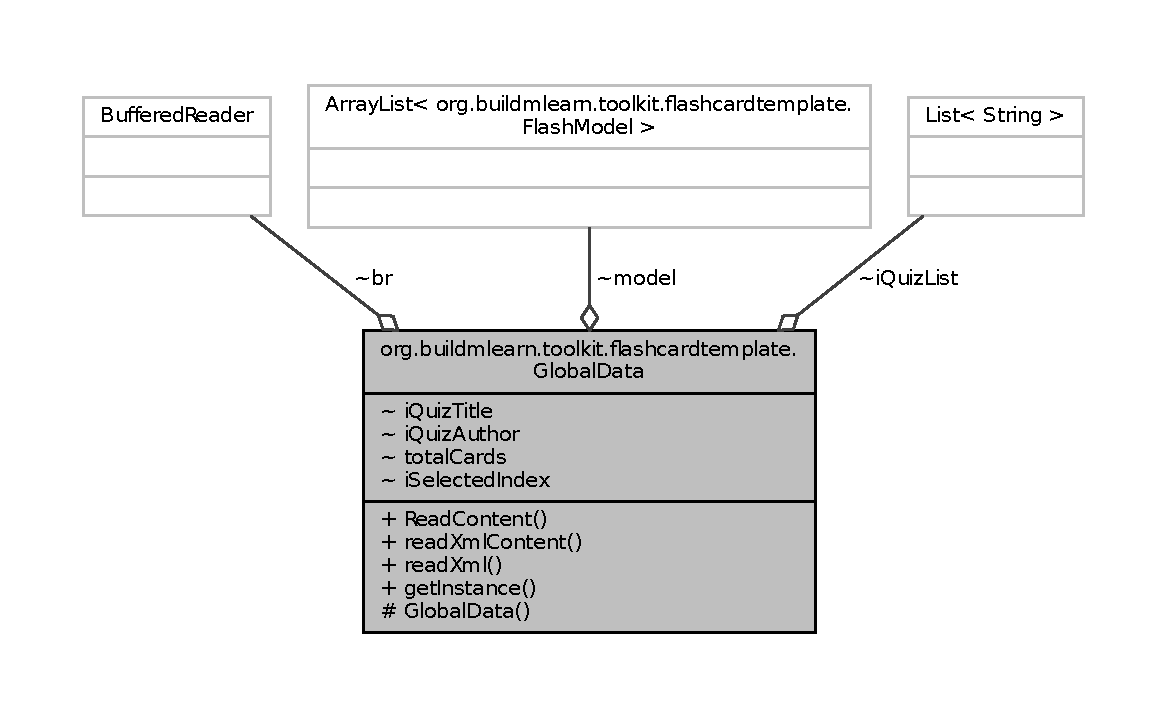
\includegraphics[width=350pt]{df/dee/classorg_1_1buildmlearn_1_1toolkit_1_1flashcardtemplate_1_1GlobalData__coll__graph}
\end{center}
\end{figure}
\subsection*{Public Member Functions}
\begin{DoxyCompactItemize}
\item 
void \hyperlink{classorg_1_1buildmlearn_1_1toolkit_1_1flashcardtemplate_1_1GlobalData_a557d8564eb6f0b690149ffaf037b9ef3}{Read\-Content} (Context my\-Context)
\item 
void \hyperlink{classorg_1_1buildmlearn_1_1toolkit_1_1flashcardtemplate_1_1GlobalData_acb83309f356c3f19a859bc9a0151ebc9}{read\-Xml\-Content} (Context my\-Context, String file\-Name)
\item 
void \hyperlink{classorg_1_1buildmlearn_1_1toolkit_1_1flashcardtemplate_1_1GlobalData_a8ff4d4f473a34a7456a3c0209d6eec0b}{read\-Xml} (String file\-Path)
\end{DoxyCompactItemize}
\subsection*{Static Public Member Functions}
\begin{DoxyCompactItemize}
\item 
static \hyperlink{classorg_1_1buildmlearn_1_1toolkit_1_1flashcardtemplate_1_1GlobalData}{Global\-Data} \hyperlink{classorg_1_1buildmlearn_1_1toolkit_1_1flashcardtemplate_1_1GlobalData_aeea7f82c54188fed27b4d243a10dca21}{get\-Instance} ()
\end{DoxyCompactItemize}
\subsection*{Protected Member Functions}
\begin{DoxyCompactItemize}
\item 
\hyperlink{classorg_1_1buildmlearn_1_1toolkit_1_1flashcardtemplate_1_1GlobalData_ac3e6ef1dde088c56d40cf6ddbd2700a0}{Global\-Data} ()
\end{DoxyCompactItemize}


\subsection{Detailed Description}
Simulator code for Flash Card Template. 

\subsection{Constructor \& Destructor Documentation}
\hypertarget{classorg_1_1buildmlearn_1_1toolkit_1_1flashcardtemplate_1_1GlobalData_ac3e6ef1dde088c56d40cf6ddbd2700a0}{\index{org\-::buildmlearn\-::toolkit\-::flashcardtemplate\-::\-Global\-Data@{org\-::buildmlearn\-::toolkit\-::flashcardtemplate\-::\-Global\-Data}!Global\-Data@{Global\-Data}}
\index{Global\-Data@{Global\-Data}!org::buildmlearn::toolkit::flashcardtemplate::GlobalData@{org\-::buildmlearn\-::toolkit\-::flashcardtemplate\-::\-Global\-Data}}
\subsubsection[{Global\-Data}]{\setlength{\rightskip}{0pt plus 5cm}org.\-buildmlearn.\-toolkit.\-flashcardtemplate.\-Global\-Data.\-Global\-Data (
\begin{DoxyParamCaption}
{}
\end{DoxyParamCaption}
)\hspace{0.3cm}{\ttfamily [protected]}}}\label{classorg_1_1buildmlearn_1_1toolkit_1_1flashcardtemplate_1_1GlobalData_ac3e6ef1dde088c56d40cf6ddbd2700a0}

\begin{DoxyCode}
71                            \{
72         \textcolor{comment}{// Exists only to defeat instantiation.}
73     \}
\end{DoxyCode}


\subsection{Member Function Documentation}
\hypertarget{classorg_1_1buildmlearn_1_1toolkit_1_1flashcardtemplate_1_1GlobalData_aeea7f82c54188fed27b4d243a10dca21}{\index{org\-::buildmlearn\-::toolkit\-::flashcardtemplate\-::\-Global\-Data@{org\-::buildmlearn\-::toolkit\-::flashcardtemplate\-::\-Global\-Data}!get\-Instance@{get\-Instance}}
\index{get\-Instance@{get\-Instance}!org::buildmlearn::toolkit::flashcardtemplate::GlobalData@{org\-::buildmlearn\-::toolkit\-::flashcardtemplate\-::\-Global\-Data}}
\subsubsection[{get\-Instance}]{\setlength{\rightskip}{0pt plus 5cm}static {\bf Global\-Data} org.\-buildmlearn.\-toolkit.\-flashcardtemplate.\-Global\-Data.\-get\-Instance (
\begin{DoxyParamCaption}
{}
\end{DoxyParamCaption}
)\hspace{0.3cm}{\ttfamily [static]}}}\label{classorg_1_1buildmlearn_1_1toolkit_1_1flashcardtemplate_1_1GlobalData_aeea7f82c54188fed27b4d243a10dca21}

\begin{DoxyCode}
75                                            \{
76         \textcolor{keywordflow}{if} (instance == null) \{
77             instance = \textcolor{keyword}{new} \hyperlink{classorg_1_1buildmlearn_1_1toolkit_1_1flashcardtemplate_1_1GlobalData_ac3e6ef1dde088c56d40cf6ddbd2700a0}{GlobalData}();
78         \}
79         \textcolor{keywordflow}{return} instance;
80     \}
\end{DoxyCode}
\hypertarget{classorg_1_1buildmlearn_1_1toolkit_1_1flashcardtemplate_1_1GlobalData_a557d8564eb6f0b690149ffaf037b9ef3}{\index{org\-::buildmlearn\-::toolkit\-::flashcardtemplate\-::\-Global\-Data@{org\-::buildmlearn\-::toolkit\-::flashcardtemplate\-::\-Global\-Data}!Read\-Content@{Read\-Content}}
\index{Read\-Content@{Read\-Content}!org::buildmlearn::toolkit::flashcardtemplate::GlobalData@{org\-::buildmlearn\-::toolkit\-::flashcardtemplate\-::\-Global\-Data}}
\subsubsection[{Read\-Content}]{\setlength{\rightskip}{0pt plus 5cm}void org.\-buildmlearn.\-toolkit.\-flashcardtemplate.\-Global\-Data.\-Read\-Content (
\begin{DoxyParamCaption}
\item[{Context}]{my\-Context}
\end{DoxyParamCaption}
)}}\label{classorg_1_1buildmlearn_1_1toolkit_1_1flashcardtemplate_1_1GlobalData_a557d8564eb6f0b690149ffaf037b9ef3}

\begin{DoxyCode}
98                                                \{
99         \textcolor{keywordflow}{try} \{
100             br = \textcolor{keyword}{new} BufferedReader(\textcolor{keyword}{new} InputStreamReader(myContext.getAssets()
101                     .open(\textcolor{stringliteral}{"flashcard\_content.txt"}))); \textcolor{comment}{// throwing a}
102             \textcolor{comment}{// FileNotFoundException?}
103             iQuizTitle = br.readLine();
104             iQuizAuthor = br.readLine();
105             String text;
106             \textcolor{keywordflow}{while} ((text = br.readLine()) != null) \{
107                 iQuizList.add(text);
108             \}
109             totalCards = iQuizList.size();
110         \} \textcolor{keywordflow}{catch} (IOException e) \{
111             e.printStackTrace();
112         \} \textcolor{keywordflow}{finally} \{
113             \textcolor{keywordflow}{try} \{
114                 br.close(); \textcolor{comment}{// stop reading}
115             \} \textcolor{keywordflow}{catch} (IOException ex) \{
116                 ex.printStackTrace();
117             \}
118         \}
119     \}
\end{DoxyCode}
\hypertarget{classorg_1_1buildmlearn_1_1toolkit_1_1flashcardtemplate_1_1GlobalData_a8ff4d4f473a34a7456a3c0209d6eec0b}{\index{org\-::buildmlearn\-::toolkit\-::flashcardtemplate\-::\-Global\-Data@{org\-::buildmlearn\-::toolkit\-::flashcardtemplate\-::\-Global\-Data}!read\-Xml@{read\-Xml}}
\index{read\-Xml@{read\-Xml}!org::buildmlearn::toolkit::flashcardtemplate::GlobalData@{org\-::buildmlearn\-::toolkit\-::flashcardtemplate\-::\-Global\-Data}}
\subsubsection[{read\-Xml}]{\setlength{\rightskip}{0pt plus 5cm}void org.\-buildmlearn.\-toolkit.\-flashcardtemplate.\-Global\-Data.\-read\-Xml (
\begin{DoxyParamCaption}
\item[{String}]{file\-Path}
\end{DoxyParamCaption}
)}}\label{classorg_1_1buildmlearn_1_1toolkit_1_1flashcardtemplate_1_1GlobalData_a8ff4d4f473a34a7456a3c0209d6eec0b}

\begin{DoxyCode}
183                                          \{
184         DocumentBuilderFactory dbf = DocumentBuilderFactory.newInstance();
185 
186         dbf.setValidating(\textcolor{keyword}{false});
187 
188         DocumentBuilder db;
189         Document doc;
190 
191 
192         \textcolor{keywordflow}{try} \{
193             model = \textcolor{keyword}{new} ArrayList<FlashModel>();
194             File fXmlFile = \textcolor{keyword}{new} File(filePath);
195             db = dbf.newDocumentBuilder();
196             doc = db.parse(fXmlFile);
197             doc.normalize();
198             \textcolor{comment}{/*}
199 \textcolor{comment}{             * NodeList app\_nodes = doc}
200 \textcolor{comment}{             * .getElementsByTagName("buildmlearn\_application");}
201 \textcolor{comment}{             */}
202             \textcolor{comment}{// NamedNodeMap node = app\_nodes.item(0).getAttributes();}
203             iQuizTitle = doc.getElementsByTagName(\textcolor{stringliteral}{"title"}).item(0)
204                     .getChildNodes().item(0).getNodeValue();
205             \textcolor{comment}{// NodeList author\_nodes = doc.getElementsByTagName("author");}
206             \textcolor{comment}{// NamedNodeMap node1 = author\_nodes.item(0).getAttributes();}
207             iQuizAuthor = doc.getElementsByTagName(\textcolor{stringliteral}{"name"}).item(0)
208                     .getChildNodes().item(0).getNodeValue();
209             ;
210             \textcolor{comment}{// node1.getNamedItem("name").getNodeValue();}
211             NodeList childNodes = doc.getElementsByTagName(\textcolor{stringliteral}{"item"});
212             \textcolor{comment}{// Log.e("tag", "childNodes" + childNodes.getLength());}
213             \textcolor{keywordflow}{for} (\textcolor{keywordtype}{int} i = 0; i < childNodes.getLength(); i++) \{
214                 FlashModel app = \textcolor{keyword}{new} FlashModel();
215 
216                 Node child = childNodes.item(i);
217 
218                 \textcolor{keywordflow}{if} (child.getNodeType() == Node.ELEMENT\_NODE) \{
219                     Element element2 = (Element) child;
220 
221                     app.setQuestion(getValue(\textcolor{stringliteral}{"question"}, element2));
222                     app.setAnswer(getValue(\textcolor{stringliteral}{"answer"}, element2));
223                     app.setHint(getValue(\textcolor{stringliteral}{"hint"}, element2));
224                     app.setBase64(getValue(\textcolor{stringliteral}{"image"}, element2));
225 
226                 \}
227                 model.add(app);
228 
229             \}
230             totalCards = model.size();
231 
232             Log.d(\textcolor{stringliteral}{"tag"}, \textcolor{stringliteral}{"totalCards"} + totalCards);
233         \} \textcolor{keywordflow}{catch} (ParserConfigurationException e) \{
234             Log.e(\textcolor{stringliteral}{"tag"}, e.getLocalizedMessage());
235             e.printStackTrace();
236         \} \textcolor{keywordflow}{catch} (FileNotFoundException e) \{
237             Log.e(\textcolor{stringliteral}{"tag"}, e.getLocalizedMessage());
238             e.printStackTrace();
239         \} \textcolor{keywordflow}{catch} (SAXException e) \{
240             Log.e(\textcolor{stringliteral}{"tag"}, e.getLocalizedMessage());
241             e.printStackTrace();
242         \} \textcolor{keywordflow}{catch} (IOException e) \{
243             Log.e(\textcolor{stringliteral}{"tag"}, e.getLocalizedMessage());
244             e.printStackTrace();
245         \}
246 
247     \}
\end{DoxyCode}
\hypertarget{classorg_1_1buildmlearn_1_1toolkit_1_1flashcardtemplate_1_1GlobalData_acb83309f356c3f19a859bc9a0151ebc9}{\index{org\-::buildmlearn\-::toolkit\-::flashcardtemplate\-::\-Global\-Data@{org\-::buildmlearn\-::toolkit\-::flashcardtemplate\-::\-Global\-Data}!read\-Xml\-Content@{read\-Xml\-Content}}
\index{read\-Xml\-Content@{read\-Xml\-Content}!org::buildmlearn::toolkit::flashcardtemplate::GlobalData@{org\-::buildmlearn\-::toolkit\-::flashcardtemplate\-::\-Global\-Data}}
\subsubsection[{read\-Xml\-Content}]{\setlength{\rightskip}{0pt plus 5cm}void org.\-buildmlearn.\-toolkit.\-flashcardtemplate.\-Global\-Data.\-read\-Xml\-Content (
\begin{DoxyParamCaption}
\item[{Context}]{my\-Context, }
\item[{String}]{file\-Name}
\end{DoxyParamCaption}
)}}\label{classorg_1_1buildmlearn_1_1toolkit_1_1flashcardtemplate_1_1GlobalData_acb83309f356c3f19a859bc9a0151ebc9}

\begin{DoxyCode}
121                                                                    \{
122         XmlPullParserFactory factory;
123         XmlPullParser parser;
124         InputStreamReader is;
125         \textcolor{keywordflow}{try} \{
126             factory = XmlPullParserFactory.newInstance();
127             \textcolor{comment}{// .setNamespaceAware(true);}
128             factory.setFeature(XmlPullParser.FEATURE\_PROCESS\_NAMESPACES, \textcolor{keyword}{false});
129 
130             parser = factory.newPullParser();
131 
132             is = \textcolor{keyword}{new} InputStreamReader(myContext.getAssets().open(fileName));
133 
134             parser.setInput(is);
135             \textcolor{keywordtype}{int} eventType = parser.getEventType();
136             FlashModel app = null;
137 
138             \textcolor{keywordflow}{while} (eventType != XmlPullParser.END\_DOCUMENT) \{
139                 String name = null;
140                 \textcolor{keywordflow}{switch} (eventType) \{
141                     \textcolor{keywordflow}{case} XmlPullParser.START\_DOCUMENT:
142                         model = \textcolor{keyword}{new} ArrayList<FlashModel>();
143                         \textcolor{keywordflow}{break};
144                     \textcolor{keywordflow}{case} XmlPullParser.START\_TAG:
145                         name = parser.getName();
146 
147                         \textcolor{keywordflow}{if} (name.equalsIgnoreCase(\textcolor{stringliteral}{"title"})) \{
148                             iQuizTitle = parser.nextText();
149                         \} \textcolor{keywordflow}{else} \textcolor{keywordflow}{if} (name.equalsIgnoreCase(\textcolor{stringliteral}{"author"})) \{
150                             iQuizAuthor = parser.nextText();
151                         \} \textcolor{keywordflow}{else} \textcolor{keywordflow}{if} (name.equalsIgnoreCase(\textcolor{stringliteral}{"item"})) \{
152                             app = \textcolor{keyword}{new} FlashModel();
153                         \} \textcolor{keywordflow}{else} \textcolor{keywordflow}{if} (app != null) \{
154                             \textcolor{keywordflow}{if} (name.equalsIgnoreCase(\textcolor{stringliteral}{"question"})) \{
155                                 app.setQuestion(parser.nextText());
156                             \} \textcolor{keywordflow}{else} \textcolor{keywordflow}{if} (name.equalsIgnoreCase(\textcolor{stringliteral}{"answer"})) \{
157                                 app.setAnswer(parser.nextText());
158                             \} \textcolor{keywordflow}{else} \textcolor{keywordflow}{if} (name.equalsIgnoreCase(\textcolor{stringliteral}{"hint"})) \{
159                                 app.setHint(parser.nextText());
160                             \} \textcolor{keywordflow}{else} \textcolor{keywordflow}{if} (name.equalsIgnoreCase(\textcolor{stringliteral}{"image"})) \{
161                                 app.setBase64(parser.nextText());
162                             \}
163                         \}
164                         \textcolor{keywordflow}{break};
165                     \textcolor{keywordflow}{case} XmlPullParser.END\_TAG:
166                         name = parser.getName();
167                         \textcolor{keywordflow}{if} (name.equalsIgnoreCase(\textcolor{stringliteral}{"item"}) && app != null) \{
168                             model.add(app);
169                             totalCards = model.size();
170                         \}
171                 \}
172                 eventType = parser.next();
173 
174             \}
175         \} \textcolor{keywordflow}{catch} (XmlPullParserException e1) \{
176             e1.printStackTrace();
177         \} \textcolor{keywordflow}{catch} (IOException e) \{
178             e.printStackTrace();
179         \}
180 
181     \}
\end{DoxyCode}


The documentation for this class was generated from the following file\-:\begin{DoxyCompactItemize}
\item 
/\-Buildm\-Learn-\/\-Toolkit-\/\-Android/source-\/code/app/src/main/java/org/buildmlearn/toolkit/flashcardtemplate/\hyperlink{flashcardtemplate_2GlobalData_8java}{Global\-Data.\-java}\end{DoxyCompactItemize}

\hypertarget{classorg_1_1buildmlearn_1_1toolkit_1_1infotemplate_1_1GlobalData}{\section{org.\-buildmlearn.\-toolkit.\-infotemplate.\-Global\-Data Class Reference}
\label{classorg_1_1buildmlearn_1_1toolkit_1_1infotemplate_1_1GlobalData}\index{org.\-buildmlearn.\-toolkit.\-infotemplate.\-Global\-Data@{org.\-buildmlearn.\-toolkit.\-infotemplate.\-Global\-Data}}
}


Simulator code for Info Template.  




Collaboration diagram for org.\-buildmlearn.\-toolkit.\-infotemplate.\-Global\-Data\-:
\nopagebreak
\begin{figure}[H]
\begin{center}
\leavevmode
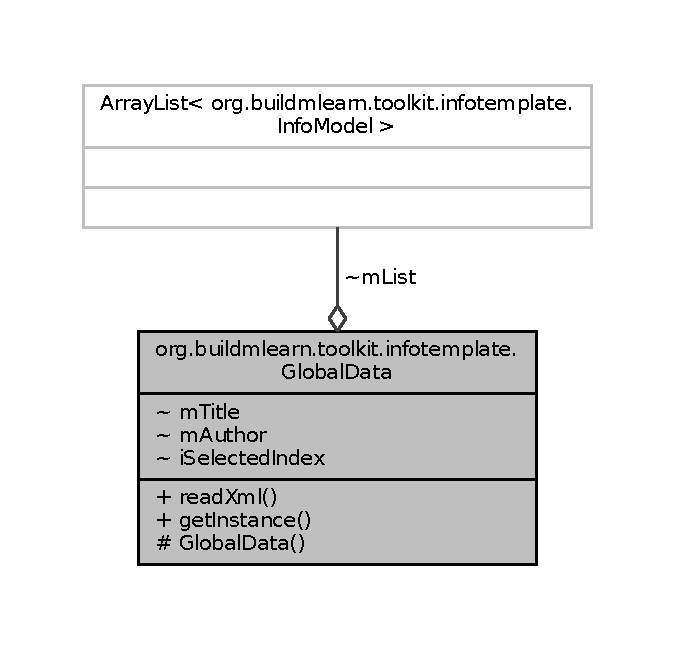
\includegraphics[width=324pt]{da/dc4/classorg_1_1buildmlearn_1_1toolkit_1_1infotemplate_1_1GlobalData__coll__graph}
\end{center}
\end{figure}
\subsection*{Public Member Functions}
\begin{DoxyCompactItemize}
\item 
void \hyperlink{classorg_1_1buildmlearn_1_1toolkit_1_1infotemplate_1_1GlobalData_abbf66139873f5feda47d3acac99d84c3}{read\-Xml} (String file\-Path)
\end{DoxyCompactItemize}
\subsection*{Static Public Member Functions}
\begin{DoxyCompactItemize}
\item 
static \hyperlink{classorg_1_1buildmlearn_1_1toolkit_1_1infotemplate_1_1GlobalData}{Global\-Data} \hyperlink{classorg_1_1buildmlearn_1_1toolkit_1_1infotemplate_1_1GlobalData_a6a01ac84ffaa2fc2fbda16b6aecf5412}{get\-Instance} ()
\end{DoxyCompactItemize}
\subsection*{Protected Member Functions}
\begin{DoxyCompactItemize}
\item 
\hyperlink{classorg_1_1buildmlearn_1_1toolkit_1_1infotemplate_1_1GlobalData_a8f07b79704ee3a40a5e501e07f6a46c0}{Global\-Data} ()
\end{DoxyCompactItemize}


\subsection{Detailed Description}
Simulator code for Info Template. 

\subsection{Constructor \& Destructor Documentation}
\hypertarget{classorg_1_1buildmlearn_1_1toolkit_1_1infotemplate_1_1GlobalData_a8f07b79704ee3a40a5e501e07f6a46c0}{\index{org\-::buildmlearn\-::toolkit\-::infotemplate\-::\-Global\-Data@{org\-::buildmlearn\-::toolkit\-::infotemplate\-::\-Global\-Data}!Global\-Data@{Global\-Data}}
\index{Global\-Data@{Global\-Data}!org::buildmlearn::toolkit::infotemplate::GlobalData@{org\-::buildmlearn\-::toolkit\-::infotemplate\-::\-Global\-Data}}
\subsubsection[{Global\-Data}]{\setlength{\rightskip}{0pt plus 5cm}org.\-buildmlearn.\-toolkit.\-infotemplate.\-Global\-Data.\-Global\-Data (
\begin{DoxyParamCaption}
{}
\end{DoxyParamCaption}
)\hspace{0.3cm}{\ttfamily [protected]}}}\label{classorg_1_1buildmlearn_1_1toolkit_1_1infotemplate_1_1GlobalData_a8f07b79704ee3a40a5e501e07f6a46c0}

\begin{DoxyCode}
57                            \{
58         \textcolor{comment}{// Exists only to defeat instantiation.}
59     \}
\end{DoxyCode}


\subsection{Member Function Documentation}
\hypertarget{classorg_1_1buildmlearn_1_1toolkit_1_1infotemplate_1_1GlobalData_a6a01ac84ffaa2fc2fbda16b6aecf5412}{\index{org\-::buildmlearn\-::toolkit\-::infotemplate\-::\-Global\-Data@{org\-::buildmlearn\-::toolkit\-::infotemplate\-::\-Global\-Data}!get\-Instance@{get\-Instance}}
\index{get\-Instance@{get\-Instance}!org::buildmlearn::toolkit::infotemplate::GlobalData@{org\-::buildmlearn\-::toolkit\-::infotemplate\-::\-Global\-Data}}
\subsubsection[{get\-Instance}]{\setlength{\rightskip}{0pt plus 5cm}static {\bf Global\-Data} org.\-buildmlearn.\-toolkit.\-infotemplate.\-Global\-Data.\-get\-Instance (
\begin{DoxyParamCaption}
{}
\end{DoxyParamCaption}
)\hspace{0.3cm}{\ttfamily [static]}}}\label{classorg_1_1buildmlearn_1_1toolkit_1_1infotemplate_1_1GlobalData_a6a01ac84ffaa2fc2fbda16b6aecf5412}

\begin{DoxyCode}
61                                            \{
62         \textcolor{keywordflow}{if} (instance == null) \{
63             instance = \textcolor{keyword}{new} \hyperlink{classorg_1_1buildmlearn_1_1toolkit_1_1infotemplate_1_1GlobalData_a8f07b79704ee3a40a5e501e07f6a46c0}{GlobalData}();
64         \}
65         \textcolor{keywordflow}{return} instance;
66     \}
\end{DoxyCode}
\hypertarget{classorg_1_1buildmlearn_1_1toolkit_1_1infotemplate_1_1GlobalData_abbf66139873f5feda47d3acac99d84c3}{\index{org\-::buildmlearn\-::toolkit\-::infotemplate\-::\-Global\-Data@{org\-::buildmlearn\-::toolkit\-::infotemplate\-::\-Global\-Data}!read\-Xml@{read\-Xml}}
\index{read\-Xml@{read\-Xml}!org::buildmlearn::toolkit::infotemplate::GlobalData@{org\-::buildmlearn\-::toolkit\-::infotemplate\-::\-Global\-Data}}
\subsubsection[{read\-Xml}]{\setlength{\rightskip}{0pt plus 5cm}void org.\-buildmlearn.\-toolkit.\-infotemplate.\-Global\-Data.\-read\-Xml (
\begin{DoxyParamCaption}
\item[{String}]{file\-Path}
\end{DoxyParamCaption}
)}}\label{classorg_1_1buildmlearn_1_1toolkit_1_1infotemplate_1_1GlobalData_abbf66139873f5feda47d3acac99d84c3}

\begin{DoxyCode}
84                                          \{
85         DocumentBuilderFactory dbf = DocumentBuilderFactory.newInstance();
86 
87         dbf.setValidating(\textcolor{keyword}{false});
88 
89         DocumentBuilder db;
90         Document doc;
91         \textcolor{keywordflow}{try} \{
92             File fXmlFile = \textcolor{keyword}{new} File(filePath);
93             mList = \textcolor{keyword}{new} ArrayList<InfoModel>();
94             db = dbf.newDocumentBuilder();
95             doc = db.parse(fXmlFile);
96             doc.normalize();
97             \textcolor{comment}{/*}
98 \textcolor{comment}{             * NodeList app\_nodes = doc
}
99 \textcolor{comment}{             * .getElementsByTagName("buildmlearn\_application");
}
100 \textcolor{comment}{             */}
101             \textcolor{comment}{// NamedNodeMap node = app\_nodes.item(0).getAttributes();}
102             mTitle = doc.getElementsByTagName(\textcolor{stringliteral}{"title"}).item(0).getChildNodes()
103                     .item(0).getNodeValue();
104             \textcolor{comment}{// NodeList author\_nodes = doc.getElementsByTagName("author");}
105             \textcolor{comment}{// NamedNodeMap node1 = author\_nodes.item(0).getAttributes();}
106             mAuthor = doc.getElementsByTagName(\textcolor{stringliteral}{"name"}).item(0).getChildNodes()
107                     .item(0).getNodeValue();
108             ;
109             \textcolor{comment}{// node1.getNamedItem("name").getNodeValue();}
110             NodeList childNodes = doc.getElementsByTagName(\textcolor{stringliteral}{"item"});
111             \textcolor{comment}{// Log.e("tag", "childNodes" + childNodes.getLength());}
112             \textcolor{keywordflow}{for} (\textcolor{keywordtype}{int} i = 0; i < childNodes.getLength(); i++) \{
113                 InfoModel app = \textcolor{keyword}{new} InfoModel();
114 
115                 Node child = childNodes.item(i);
116 
117                 \textcolor{keywordflow}{if} (child.getNodeType() == Node.ELEMENT\_NODE) \{
118                     Element element2 = (Element) child;
119 
120                     app.setInfo\_object(getValue(\textcolor{stringliteral}{"item\_title"}, element2));
121                     app.setInfo\_description(getValue(\textcolor{stringliteral}{"item\_description"}, element2));
122 
123                 \}
124                 mList.add(app);
125 
126             \}
127         \} \textcolor{keywordflow}{catch} (ParserConfigurationException e) \{
128             Log.e(\textcolor{stringliteral}{"tag"}, e.getLocalizedMessage());
129             e.printStackTrace();
130         \} \textcolor{keywordflow}{catch} (FileNotFoundException e) \{
131             Log.e(\textcolor{stringliteral}{"tag"}, e.getLocalizedMessage());
132             e.printStackTrace();
133         \} \textcolor{keywordflow}{catch} (SAXException e) \{
134             Log.e(\textcolor{stringliteral}{"tag"}, e.getLocalizedMessage());
135             e.printStackTrace();
136         \} \textcolor{keywordflow}{catch} (IOException e) \{
137             Log.e(\textcolor{stringliteral}{"tag"}, e.getLocalizedMessage());
138             e.printStackTrace();
139         \}
140 
141     \}
\end{DoxyCode}


The documentation for this class was generated from the following file\-:\begin{DoxyCompactItemize}
\item 
/\-Buildm\-Learn-\/\-Toolkit-\/\-Android/source-\/code/app/src/main/java/org/buildmlearn/toolkit/infotemplate/\hyperlink{infotemplate_2GlobalData_8java}{Global\-Data.\-java}\end{DoxyCompactItemize}

\hypertarget{classorg_1_1buildmlearn_1_1toolkit_1_1quiztemplate_1_1GlobalData}{\section{org.\-buildmlearn.\-toolkit.\-quiztemplate.\-Global\-Data Class Reference}
\label{classorg_1_1buildmlearn_1_1toolkit_1_1quiztemplate_1_1GlobalData}\index{org.\-buildmlearn.\-toolkit.\-quiztemplate.\-Global\-Data@{org.\-buildmlearn.\-toolkit.\-quiztemplate.\-Global\-Data}}
}


Simulator code for Quiz Template.  




Collaboration diagram for org.\-buildmlearn.\-toolkit.\-quiztemplate.\-Global\-Data\-:
\nopagebreak
\begin{figure}[H]
\begin{center}
\leavevmode
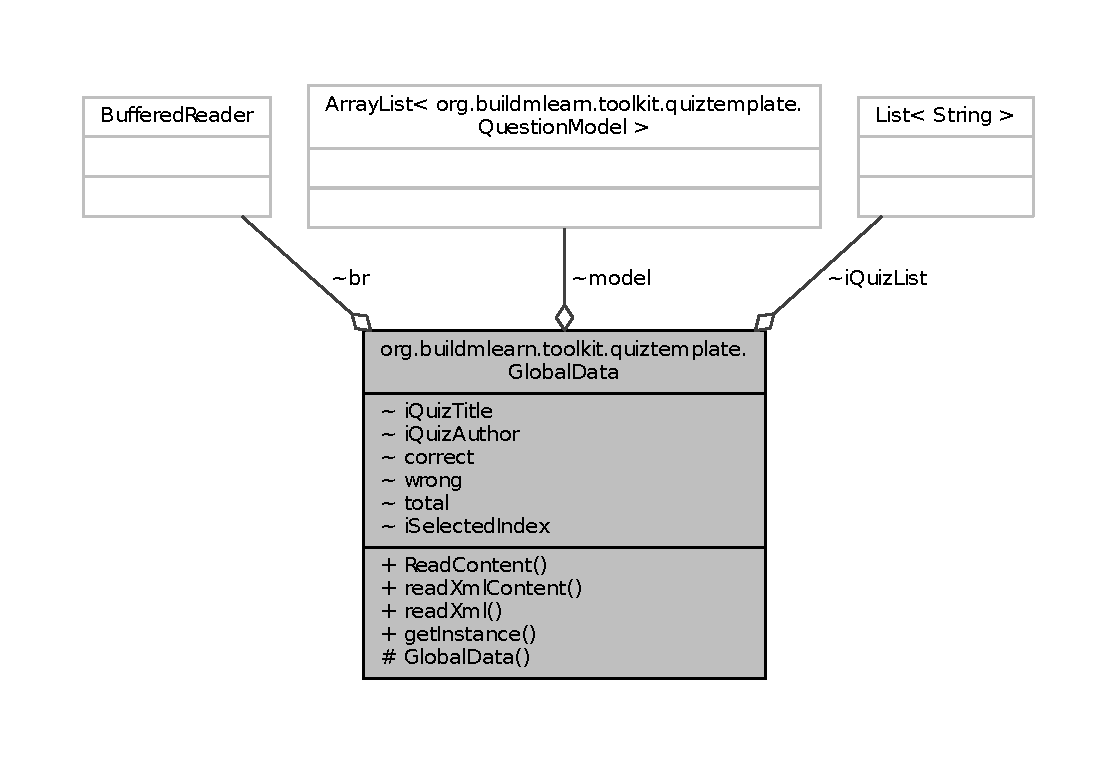
\includegraphics[width=350pt]{db/db2/classorg_1_1buildmlearn_1_1toolkit_1_1quiztemplate_1_1GlobalData__coll__graph}
\end{center}
\end{figure}
\subsection*{Public Member Functions}
\begin{DoxyCompactItemize}
\item 
void \hyperlink{classorg_1_1buildmlearn_1_1toolkit_1_1quiztemplate_1_1GlobalData_aedd79ff6db8cfbf154c09f911f3b1c46}{Read\-Content} (Context my\-Context)
\item 
void \hyperlink{classorg_1_1buildmlearn_1_1toolkit_1_1quiztemplate_1_1GlobalData_abed3c168b313ac617f44e640d9c572bc}{read\-Xml\-Content} (Context my\-Context, String file\-Name)
\item 
void \hyperlink{classorg_1_1buildmlearn_1_1toolkit_1_1quiztemplate_1_1GlobalData_a77c7ed0e4d625559c4bcb92249e27ed7}{read\-Xml} (String file\-Path)
\end{DoxyCompactItemize}
\subsection*{Static Public Member Functions}
\begin{DoxyCompactItemize}
\item 
static \hyperlink{classorg_1_1buildmlearn_1_1toolkit_1_1quiztemplate_1_1GlobalData}{Global\-Data} \hyperlink{classorg_1_1buildmlearn_1_1toolkit_1_1quiztemplate_1_1GlobalData_a43169ec5782adad2b277766a3dbe5085}{get\-Instance} ()
\end{DoxyCompactItemize}
\subsection*{Protected Member Functions}
\begin{DoxyCompactItemize}
\item 
\hyperlink{classorg_1_1buildmlearn_1_1toolkit_1_1quiztemplate_1_1GlobalData_ac2accaa89bbcf8c4da931945de046ca7}{Global\-Data} ()
\end{DoxyCompactItemize}


\subsection{Detailed Description}
Simulator code for Quiz Template. 

\subsection{Constructor \& Destructor Documentation}
\hypertarget{classorg_1_1buildmlearn_1_1toolkit_1_1quiztemplate_1_1GlobalData_ac2accaa89bbcf8c4da931945de046ca7}{\index{org\-::buildmlearn\-::toolkit\-::quiztemplate\-::\-Global\-Data@{org\-::buildmlearn\-::toolkit\-::quiztemplate\-::\-Global\-Data}!Global\-Data@{Global\-Data}}
\index{Global\-Data@{Global\-Data}!org::buildmlearn::toolkit::quiztemplate::GlobalData@{org\-::buildmlearn\-::toolkit\-::quiztemplate\-::\-Global\-Data}}
\subsubsection[{Global\-Data}]{\setlength{\rightskip}{0pt plus 5cm}org.\-buildmlearn.\-toolkit.\-quiztemplate.\-Global\-Data.\-Global\-Data (
\begin{DoxyParamCaption}
{}
\end{DoxyParamCaption}
)\hspace{0.3cm}{\ttfamily [protected]}}}\label{classorg_1_1buildmlearn_1_1toolkit_1_1quiztemplate_1_1GlobalData_ac2accaa89bbcf8c4da931945de046ca7}

\begin{DoxyCode}
73                            \{
74         \textcolor{comment}{// Exists only to defeat instantiation.}
75     \}
\end{DoxyCode}


\subsection{Member Function Documentation}
\hypertarget{classorg_1_1buildmlearn_1_1toolkit_1_1quiztemplate_1_1GlobalData_a43169ec5782adad2b277766a3dbe5085}{\index{org\-::buildmlearn\-::toolkit\-::quiztemplate\-::\-Global\-Data@{org\-::buildmlearn\-::toolkit\-::quiztemplate\-::\-Global\-Data}!get\-Instance@{get\-Instance}}
\index{get\-Instance@{get\-Instance}!org::buildmlearn::toolkit::quiztemplate::GlobalData@{org\-::buildmlearn\-::toolkit\-::quiztemplate\-::\-Global\-Data}}
\subsubsection[{get\-Instance}]{\setlength{\rightskip}{0pt plus 5cm}static {\bf Global\-Data} org.\-buildmlearn.\-toolkit.\-quiztemplate.\-Global\-Data.\-get\-Instance (
\begin{DoxyParamCaption}
{}
\end{DoxyParamCaption}
)\hspace{0.3cm}{\ttfamily [static]}}}\label{classorg_1_1buildmlearn_1_1toolkit_1_1quiztemplate_1_1GlobalData_a43169ec5782adad2b277766a3dbe5085}

\begin{DoxyCode}
77                                            \{
78         \textcolor{keywordflow}{if} (instance == null) \{
79             instance = \textcolor{keyword}{new} \hyperlink{classorg_1_1buildmlearn_1_1toolkit_1_1quiztemplate_1_1GlobalData_ac2accaa89bbcf8c4da931945de046ca7}{GlobalData}();
80         \}
81         \textcolor{keywordflow}{return} instance;
82     \}
\end{DoxyCode}
\hypertarget{classorg_1_1buildmlearn_1_1toolkit_1_1quiztemplate_1_1GlobalData_aedd79ff6db8cfbf154c09f911f3b1c46}{\index{org\-::buildmlearn\-::toolkit\-::quiztemplate\-::\-Global\-Data@{org\-::buildmlearn\-::toolkit\-::quiztemplate\-::\-Global\-Data}!Read\-Content@{Read\-Content}}
\index{Read\-Content@{Read\-Content}!org::buildmlearn::toolkit::quiztemplate::GlobalData@{org\-::buildmlearn\-::toolkit\-::quiztemplate\-::\-Global\-Data}}
\subsubsection[{Read\-Content}]{\setlength{\rightskip}{0pt plus 5cm}void org.\-buildmlearn.\-toolkit.\-quiztemplate.\-Global\-Data.\-Read\-Content (
\begin{DoxyParamCaption}
\item[{Context}]{my\-Context}
\end{DoxyParamCaption}
)}}\label{classorg_1_1buildmlearn_1_1toolkit_1_1quiztemplate_1_1GlobalData_aedd79ff6db8cfbf154c09f911f3b1c46}

\begin{DoxyCode}
100                                                \{
101         \textcolor{keywordflow}{try} \{
102             br = \textcolor{keyword}{new} BufferedReader(\textcolor{keyword}{new} InputStreamReader(myContext.getAssets()
103                     .open(\textcolor{stringliteral}{"quiz\_content.txt"}))); \textcolor{comment}{// throwing a}
104             \textcolor{comment}{// FileNotFoundException?}
105             iQuizTitle = br.readLine();
106             iQuizAuthor = br.readLine();
107             String text;
108             \textcolor{keywordflow}{while} ((text = br.readLine()) != null) \{
109                 iQuizList.add(text);
110             \}
111             total = iQuizList.size();
112         \} \textcolor{keywordflow}{catch} (IOException e) \{
113             e.printStackTrace();
114         \} \textcolor{keywordflow}{finally} \{
115             \textcolor{keywordflow}{try} \{
116                 br.close(); \textcolor{comment}{// stop reading}
117             \} \textcolor{keywordflow}{catch} (IOException ex) \{
118                 ex.printStackTrace();
119             \}
120         \}
121     \}
\end{DoxyCode}
\hypertarget{classorg_1_1buildmlearn_1_1toolkit_1_1quiztemplate_1_1GlobalData_a77c7ed0e4d625559c4bcb92249e27ed7}{\index{org\-::buildmlearn\-::toolkit\-::quiztemplate\-::\-Global\-Data@{org\-::buildmlearn\-::toolkit\-::quiztemplate\-::\-Global\-Data}!read\-Xml@{read\-Xml}}
\index{read\-Xml@{read\-Xml}!org::buildmlearn::toolkit::quiztemplate::GlobalData@{org\-::buildmlearn\-::toolkit\-::quiztemplate\-::\-Global\-Data}}
\subsubsection[{read\-Xml}]{\setlength{\rightskip}{0pt plus 5cm}void org.\-buildmlearn.\-toolkit.\-quiztemplate.\-Global\-Data.\-read\-Xml (
\begin{DoxyParamCaption}
\item[{String}]{file\-Path}
\end{DoxyParamCaption}
)}}\label{classorg_1_1buildmlearn_1_1toolkit_1_1quiztemplate_1_1GlobalData_a77c7ed0e4d625559c4bcb92249e27ed7}

\begin{DoxyCode}
188                                          \{
189         DocumentBuilderFactory dbf = DocumentBuilderFactory.newInstance();
190 
191         dbf.setValidating(\textcolor{keyword}{false});
192 
193         ArrayList<String> mOptions = null;
194         DocumentBuilder db;
195         Document doc;
196         \textcolor{keywordflow}{try} \{
197             File fXmlFile = \textcolor{keyword}{new} File(filePath);
198             model = \textcolor{keyword}{new} ArrayList<QuestionModel>();
199             db = dbf.newDocumentBuilder();
200             doc = db.parse(fXmlFile);
201             doc.normalize();
202             iQuizTitle = doc.getElementsByTagName(\textcolor{stringliteral}{"title"}).item(0)
203                     .getChildNodes().item(0).getNodeValue();
204             iQuizAuthor = doc.getElementsByTagName(\textcolor{stringliteral}{"name"}).item(0)
205                     .getChildNodes().item(0).getNodeValue();
206             NodeList childNodes = doc.getElementsByTagName(\textcolor{stringliteral}{"item"});
207             \textcolor{comment}{// Log.e("tag", "childNodes" + childNodes.getLength());}
208             \textcolor{keywordflow}{for} (\textcolor{keywordtype}{int} i = 0; i < childNodes.getLength(); i++) \{
209                 QuestionModel app = \textcolor{keyword}{new} QuestionModel();
210 
211                 Node child = childNodes.item(i);
212 
213                 \textcolor{keywordflow}{if} (child.getNodeType() == Node.ELEMENT\_NODE) \{
214                     Element element2 = (Element) child;
215 
216                     app.setQuestion(getValue(\textcolor{stringliteral}{"question"}, element2));
217                     mOptions = \textcolor{keyword}{new} ArrayList<String>();
218                     NodeList optionNodes = element2
219                             .getElementsByTagName(\textcolor{stringliteral}{"option"});
220                     \textcolor{keywordflow}{for} (\textcolor{keywordtype}{int} j = 0; j < optionNodes.getLength(); j++) \{
221                         mOptions.add(optionNodes.item(j).getChildNodes().item(0).getNodeValue());
222                     \}
223                     app.setAnswer(getValue(\textcolor{stringliteral}{"answer"}, element2));
224                     app.setOptions(mOptions);
225                 \}
226                 model.add(app);
227             \}
228             total = model.size();
229 
230         \} \textcolor{keywordflow}{catch} (ParserConfigurationException e) \{
231             Log.e(\textcolor{stringliteral}{"tag"}, e.getLocalizedMessage());
232             e.printStackTrace();
233         \} \textcolor{keywordflow}{catch} (FileNotFoundException e) \{
234             Log.e(\textcolor{stringliteral}{"tag"}, e.getLocalizedMessage());
235             e.printStackTrace();
236         \} \textcolor{keywordflow}{catch} (SAXException e) \{
237             Log.e(\textcolor{stringliteral}{"tag"}, e.getLocalizedMessage());
238             e.printStackTrace();
239         \} \textcolor{keywordflow}{catch} (IOException e) \{
240             Log.e(\textcolor{stringliteral}{"tag"}, e.getLocalizedMessage());
241             e.printStackTrace();
242         \}
243 
244     \}
\end{DoxyCode}
\hypertarget{classorg_1_1buildmlearn_1_1toolkit_1_1quiztemplate_1_1GlobalData_abed3c168b313ac617f44e640d9c572bc}{\index{org\-::buildmlearn\-::toolkit\-::quiztemplate\-::\-Global\-Data@{org\-::buildmlearn\-::toolkit\-::quiztemplate\-::\-Global\-Data}!read\-Xml\-Content@{read\-Xml\-Content}}
\index{read\-Xml\-Content@{read\-Xml\-Content}!org::buildmlearn::toolkit::quiztemplate::GlobalData@{org\-::buildmlearn\-::toolkit\-::quiztemplate\-::\-Global\-Data}}
\subsubsection[{read\-Xml\-Content}]{\setlength{\rightskip}{0pt plus 5cm}void org.\-buildmlearn.\-toolkit.\-quiztemplate.\-Global\-Data.\-read\-Xml\-Content (
\begin{DoxyParamCaption}
\item[{Context}]{my\-Context, }
\item[{String}]{file\-Name}
\end{DoxyParamCaption}
)}}\label{classorg_1_1buildmlearn_1_1toolkit_1_1quiztemplate_1_1GlobalData_abed3c168b313ac617f44e640d9c572bc}

\begin{DoxyCode}
123                                                                    \{
124         XmlPullParserFactory factory;
125         XmlPullParser parser;
126         InputStreamReader is;
127         ArrayList<String> mOptions = null;
128         \textcolor{keywordflow}{try} \{
129             factory = XmlPullParserFactory.newInstance();
130             \textcolor{comment}{// .setNamespaceAware(true);}
131             factory.setFeature(XmlPullParser.FEATURE\_PROCESS\_NAMESPACES, \textcolor{keyword}{false});
132 
133             parser = factory.newPullParser();
134 
135             is = \textcolor{keyword}{new} InputStreamReader(myContext.getAssets().open(fileName));
136 
137             parser.setInput(is);
138             \textcolor{keywordtype}{int} eventType = parser.getEventType();
139             QuestionModel app = null;
140 
141             \textcolor{keywordflow}{while} (eventType != XmlPullParser.END\_DOCUMENT) \{
142                 String name = null;
143                 \textcolor{keywordflow}{switch} (eventType) \{
144                     \textcolor{keywordflow}{case} XmlPullParser.START\_DOCUMENT:
145                         model = \textcolor{keyword}{new} ArrayList<QuestionModel>();
146                         \textcolor{keywordflow}{break};
147                     \textcolor{keywordflow}{case} XmlPullParser.START\_TAG:
148                         name = parser.getName();
149 
150                         \textcolor{keywordflow}{if} (name.equalsIgnoreCase(\textcolor{stringliteral}{"title"})) \{
151                             iQuizTitle = parser.nextText();
152                         \} \textcolor{keywordflow}{else} \textcolor{keywordflow}{if} (name.equalsIgnoreCase(\textcolor{stringliteral}{"author"})) \{
153                             iQuizAuthor = parser.nextText();
154                         \} \textcolor{keywordflow}{else} \textcolor{keywordflow}{if} (name.equalsIgnoreCase(\textcolor{stringliteral}{"item"})) \{
155                             app = \textcolor{keyword}{new} QuestionModel();
156                             mOptions = \textcolor{keyword}{new} ArrayList<String>();
157                         \} \textcolor{keywordflow}{else} \textcolor{keywordflow}{if} (app != null) \{
158                             \textcolor{keywordflow}{if} (name.equalsIgnoreCase(\textcolor{stringliteral}{"question"})) \{
159                                 app.setQuestion(parser.nextText());
160                             \} \textcolor{keywordflow}{else} \textcolor{keywordflow}{if} (name.equalsIgnoreCase(\textcolor{stringliteral}{"option"})) \{
161                                 mOptions.add(parser.nextText());
162                                 app.setOptions(mOptions);
163                             \} \textcolor{keywordflow}{else} \textcolor{keywordflow}{if} (name.equalsIgnoreCase(\textcolor{stringliteral}{"answer"})) \{
164                                 app.setAnswer(parser.nextText());
165                             \}
166                         \}
167                         \textcolor{keywordflow}{break};
168                     \textcolor{keywordflow}{case} XmlPullParser.END\_TAG:
169                         name = parser.getName();
170                         \textcolor{keywordflow}{if} (name.equalsIgnoreCase(\textcolor{stringliteral}{"item"}) && app != null) \{
171                             model.add(app);
172                             total = model.size();
173                         \}
174                 \}
175                 eventType = parser.next();
176 
177             \}
178         \} \textcolor{keywordflow}{catch} (XmlPullParserException e1) \{
179             e1.printStackTrace();
180         \} \textcolor{keywordflow}{catch} (IOException e) \{
181             e.printStackTrace();
182         \}
183         \textcolor{comment}{// return model;}
184         \textcolor{comment}{// BuildmLearnModel.getInstance(myContext).setAllAppsList(model);}
185 
186     \}
\end{DoxyCode}


The documentation for this class was generated from the following file\-:\begin{DoxyCompactItemize}
\item 
/\-Buildm\-Learn-\/\-Toolkit-\/\-Android/source-\/code/app/src/main/java/org/buildmlearn/toolkit/quiztemplate/\hyperlink{quiztemplate_2GlobalData_8java}{Global\-Data.\-java}\end{DoxyCompactItemize}

\hypertarget{classorg_1_1buildmlearn_1_1toolkit_1_1templates_1_1FlashCardAdapter_1_1Holder}{\section{org.\-buildmlearn.\-toolkit.\-templates.\-Flash\-Card\-Adapter.\-Holder Class Reference}
\label{classorg_1_1buildmlearn_1_1toolkit_1_1templates_1_1FlashCardAdapter_1_1Holder}\index{org.\-buildmlearn.\-toolkit.\-templates.\-Flash\-Card\-Adapter.\-Holder@{org.\-buildmlearn.\-toolkit.\-templates.\-Flash\-Card\-Adapter.\-Holder}}
}


Collaboration diagram for org.\-buildmlearn.\-toolkit.\-templates.\-Flash\-Card\-Adapter.\-Holder\-:
\nopagebreak
\begin{figure}[H]
\begin{center}
\leavevmode
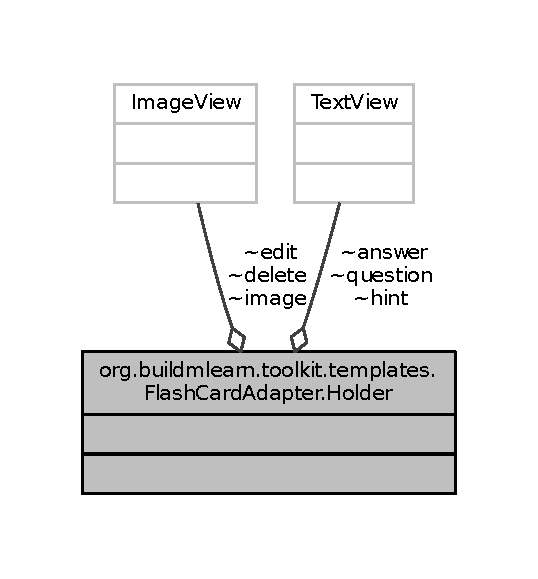
\includegraphics[width=258pt]{d1/d30/classorg_1_1buildmlearn_1_1toolkit_1_1templates_1_1FlashCardAdapter_1_1Holder__coll__graph}
\end{center}
\end{figure}


The documentation for this class was generated from the following file\-:\begin{DoxyCompactItemize}
\item 
/\-Buildm\-Learn-\/\-Toolkit-\/\-Android/source-\/code/app/src/main/java/org/buildmlearn/toolkit/templates/\hyperlink{FlashCardAdapter_8java}{Flash\-Card\-Adapter.\-java}\end{DoxyCompactItemize}

\hypertarget{classorg_1_1buildmlearn_1_1toolkit_1_1templates_1_1QuizAdapter_1_1Holder}{\section{org.\-buildmlearn.\-toolkit.\-templates.\-Quiz\-Adapter.\-Holder Class Reference}
\label{classorg_1_1buildmlearn_1_1toolkit_1_1templates_1_1QuizAdapter_1_1Holder}\index{org.\-buildmlearn.\-toolkit.\-templates.\-Quiz\-Adapter.\-Holder@{org.\-buildmlearn.\-toolkit.\-templates.\-Quiz\-Adapter.\-Holder}}
}


Collaboration diagram for org.\-buildmlearn.\-toolkit.\-templates.\-Quiz\-Adapter.\-Holder\-:
\nopagebreak
\begin{figure}[H]
\begin{center}
\leavevmode
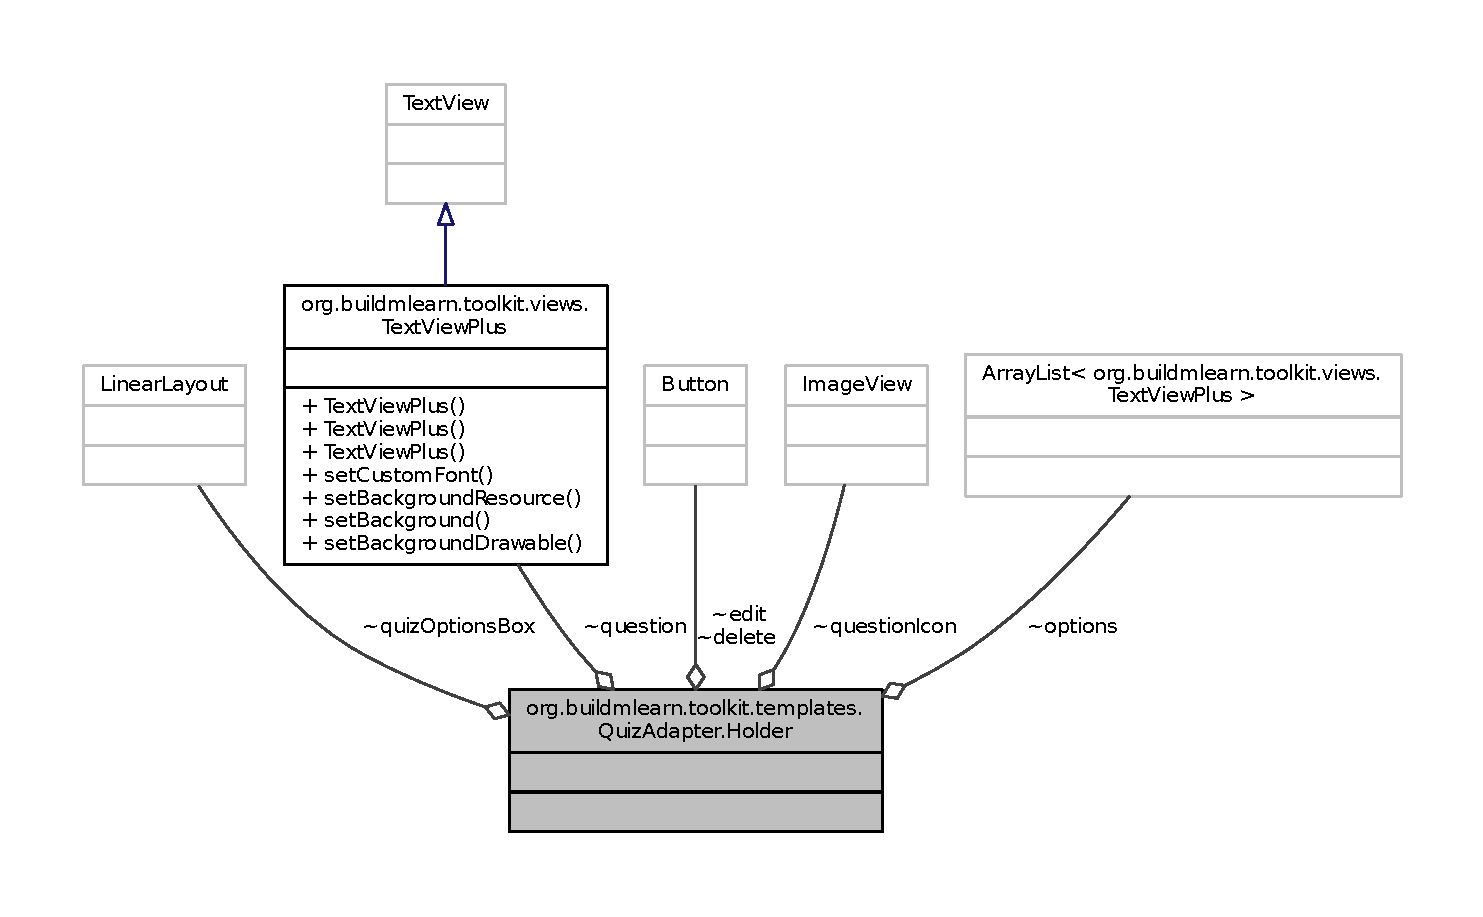
\includegraphics[width=350pt]{d0/d2e/classorg_1_1buildmlearn_1_1toolkit_1_1templates_1_1QuizAdapter_1_1Holder__coll__graph}
\end{center}
\end{figure}


The documentation for this class was generated from the following file\-:\begin{DoxyCompactItemize}
\item 
/\-Buildm\-Learn-\/\-Toolkit-\/\-Android/source-\/code/app/src/main/java/org/buildmlearn/toolkit/templates/\hyperlink{QuizAdapter_8java}{Quiz\-Adapter.\-java}\end{DoxyCompactItemize}

\hypertarget{classorg_1_1buildmlearn_1_1toolkit_1_1activity_1_1HomeActivity}{\section{org.\-buildmlearn.\-toolkit.\-activity.\-Home\-Activity Class Reference}
\label{classorg_1_1buildmlearn_1_1toolkit_1_1activity_1_1HomeActivity}\index{org.\-buildmlearn.\-toolkit.\-activity.\-Home\-Activity@{org.\-buildmlearn.\-toolkit.\-activity.\-Home\-Activity}}
}


Home screen of the application containg all the menus and settings.  




Inheritance diagram for org.\-buildmlearn.\-toolkit.\-activity.\-Home\-Activity\-:
\nopagebreak
\begin{figure}[H]
\begin{center}
\leavevmode
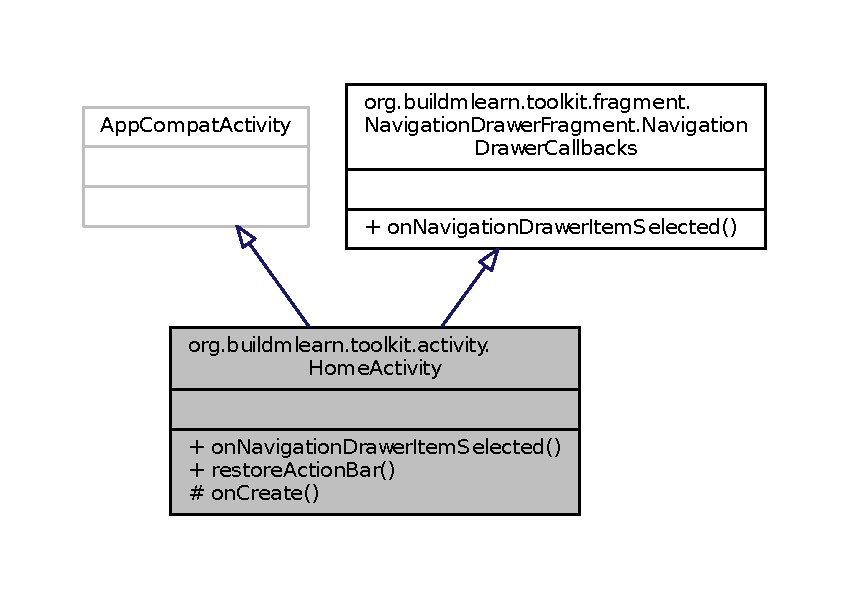
\includegraphics[width=350pt]{dd/d80/classorg_1_1buildmlearn_1_1toolkit_1_1activity_1_1HomeActivity__inherit__graph}
\end{center}
\end{figure}


Collaboration diagram for org.\-buildmlearn.\-toolkit.\-activity.\-Home\-Activity\-:
\nopagebreak
\begin{figure}[H]
\begin{center}
\leavevmode
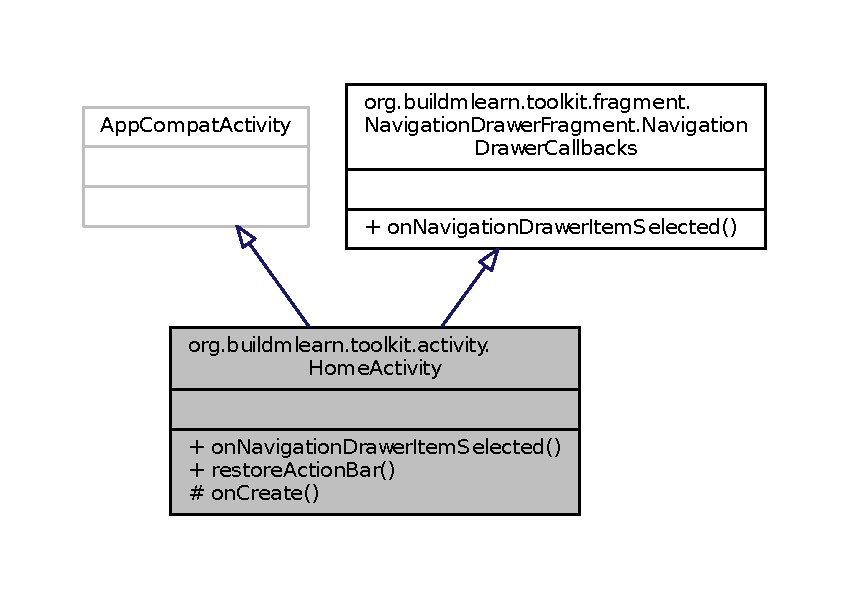
\includegraphics[width=350pt]{d3/d43/classorg_1_1buildmlearn_1_1toolkit_1_1activity_1_1HomeActivity__coll__graph}
\end{center}
\end{figure}
\subsection*{Public Member Functions}
\begin{DoxyCompactItemize}
\item 
void \hyperlink{classorg_1_1buildmlearn_1_1toolkit_1_1activity_1_1HomeActivity_af75c80f626f8c3a7141c046108ff229f}{on\-Navigation\-Drawer\-Item\-Selected} (int position)
\item 
void \hyperlink{classorg_1_1buildmlearn_1_1toolkit_1_1activity_1_1HomeActivity_acd6a4343ee19b57250586b50bcafe8ae}{restore\-Action\-Bar} ()
\end{DoxyCompactItemize}
\subsection*{Protected Member Functions}
\begin{DoxyCompactItemize}
\item 
void \hyperlink{classorg_1_1buildmlearn_1_1toolkit_1_1activity_1_1HomeActivity_a84a92cce3842759b4e3c18ecefbe2ced}{on\-Create} (Bundle saved\-Instance\-State)
\end{DoxyCompactItemize}


\subsection{Detailed Description}
Home screen of the application containg all the menus and settings. 

\subsection{Member Function Documentation}
\hypertarget{classorg_1_1buildmlearn_1_1toolkit_1_1activity_1_1HomeActivity_a84a92cce3842759b4e3c18ecefbe2ced}{\index{org\-::buildmlearn\-::toolkit\-::activity\-::\-Home\-Activity@{org\-::buildmlearn\-::toolkit\-::activity\-::\-Home\-Activity}!on\-Create@{on\-Create}}
\index{on\-Create@{on\-Create}!org::buildmlearn::toolkit::activity::HomeActivity@{org\-::buildmlearn\-::toolkit\-::activity\-::\-Home\-Activity}}
\subsubsection[{on\-Create}]{\setlength{\rightskip}{0pt plus 5cm}void org.\-buildmlearn.\-toolkit.\-activity.\-Home\-Activity.\-on\-Create (
\begin{DoxyParamCaption}
\item[{Bundle}]{saved\-Instance\-State}
\end{DoxyParamCaption}
)\hspace{0.3cm}{\ttfamily [protected]}}}\label{classorg_1_1buildmlearn_1_1toolkit_1_1activity_1_1HomeActivity_a84a92cce3842759b4e3c18ecefbe2ced}

\begin{DoxyCode}
43                                                        \{
44         super.onCreate(savedInstanceState);
45 
46         Fabric.with(\textcolor{keyword}{this}, \textcolor{keyword}{new} Crashlytics());
47 
48         setContentView(R.layout.activity\_home);
49         setSupportActionBar((Toolbar) findViewById(R.id.toolbar));
50 
51         mNavigationDrawerFragment = (NavigationDrawerFragment)
52                 getSupportFragmentManager().findFragmentById(R.id.navigation\_drawer);
53         mTitle = getTitle();
54 
55         \textcolor{comment}{// Set up the drawer.}
56         mNavigationDrawerFragment.setUp(
57                 R.id.navigation\_drawer,
58                 (DrawerLayout) findViewById(R.id.drawer\_layout));
59 
60     \}
\end{DoxyCode}
\hypertarget{classorg_1_1buildmlearn_1_1toolkit_1_1activity_1_1HomeActivity_af75c80f626f8c3a7141c046108ff229f}{\index{org\-::buildmlearn\-::toolkit\-::activity\-::\-Home\-Activity@{org\-::buildmlearn\-::toolkit\-::activity\-::\-Home\-Activity}!on\-Navigation\-Drawer\-Item\-Selected@{on\-Navigation\-Drawer\-Item\-Selected}}
\index{on\-Navigation\-Drawer\-Item\-Selected@{on\-Navigation\-Drawer\-Item\-Selected}!org::buildmlearn::toolkit::activity::HomeActivity@{org\-::buildmlearn\-::toolkit\-::activity\-::\-Home\-Activity}}
\subsubsection[{on\-Navigation\-Drawer\-Item\-Selected}]{\setlength{\rightskip}{0pt plus 5cm}void org.\-buildmlearn.\-toolkit.\-activity.\-Home\-Activity.\-on\-Navigation\-Drawer\-Item\-Selected (
\begin{DoxyParamCaption}
\item[{int}]{position}
\end{DoxyParamCaption}
)}}\label{classorg_1_1buildmlearn_1_1toolkit_1_1activity_1_1HomeActivity_af75c80f626f8c3a7141c046108ff229f}
Called when an item in the navigation drawer is selected. 

Implements \hyperlink{interfaceorg_1_1buildmlearn_1_1toolkit_1_1fragment_1_1NavigationDrawerFragment_1_1NavigationDrawerCallbacks_a6068a4dec53d00ec47c222f995064e6c}{org.\-buildmlearn.\-toolkit.\-fragment.\-Navigation\-Drawer\-Fragment.\-Navigation\-Drawer\-Callbacks}.


\begin{DoxyCode}
66                                                              \{
67         Section[] menuItem = Section.values();
68         Section selectedMenuItem = menuItem[position];
69         \textcolor{keywordflow}{if} (selectedMenuItem.getType() == \hyperlink{enumorg_1_1buildmlearn_1_1toolkit_1_1model_1_1Section_a9afae152c2f7c91883417b9de909da27}{Section.ACTIVITY}) \{
70             Class<?> c;
71             \textcolor{keywordflow}{if} (selectedMenuItem.getViewName() != null) \{
72                 \textcolor{keywordflow}{try} \{
73                     c = Class.forName(selectedMenuItem.getViewName());
74                     Intent intent = \textcolor{keyword}{new} Intent(\textcolor{keyword}{this}, c);
75                     startActivity(intent);
76 
77                 \} \textcolor{keywordflow}{catch} (ClassNotFoundException e) \{
78                     Toast.makeText(\textcolor{keyword}{this}, e.getLocalizedMessage(), Toast.LENGTH\_LONG).show();
79                     e.printStackTrace();
80                 \}
81             \}
82         \} \textcolor{keywordflow}{else} \textcolor{keywordflow}{if} (selectedMenuItem.getType() == \hyperlink{enumorg_1_1buildmlearn_1_1toolkit_1_1model_1_1Section_a536f7f08eb441bb4af16270238999cc4}{Section.FRAGMENT}) \{
83             \textcolor{keywordflow}{if} (currentSection == null || selectedMenuItem != currentSection) \{
84                 currentSection = selectedMenuItem;
85                 FragmentManager fm = getFragmentManager();
86                 FragmentTransaction ft = fm.beginTransaction().setTransition(FragmentTransaction.
      TRANSIT\_FRAGMENT\_FADE);
87                 Fragment f = fm.findFragmentById(R.id.container);
88                 \textcolor{keywordflow}{if} (f != null) \{
89                     \textcolor{keywordflow}{if} (currentSection.\hyperlink{enumorg_1_1buildmlearn_1_1toolkit_1_1model_1_1Section_ae9b75c2d499a28b4aa0ee59fa73810f2}{isKeep}()) \{
90                         ft.detach(f);
91                     \} \textcolor{keywordflow}{else} \{
92                         ft.remove(f);
93                     \}
94                 \}
95                 String fragmentClassName = currentSection.getViewName();
96                 \textcolor{keywordflow}{if} (currentSection.\hyperlink{enumorg_1_1buildmlearn_1_1toolkit_1_1model_1_1Section_ae9b75c2d499a28b4aa0ee59fa73810f2}{isKeep}() && ((f = fm.findFragmentByTag(fragmentClassName)) != null
      )) \{
97                     ft.attach(f);
98                 \} \textcolor{keywordflow}{else} \{
99                     f = Fragment.instantiate(\textcolor{keyword}{this}, fragmentClassName);
100                     ft.add(R.id.container, f, fragmentClassName);
101                 \}
102                 ft.commit();
103 
104 
105             \}
106         \}
107     \}
\end{DoxyCode}
\hypertarget{classorg_1_1buildmlearn_1_1toolkit_1_1activity_1_1HomeActivity_acd6a4343ee19b57250586b50bcafe8ae}{\index{org\-::buildmlearn\-::toolkit\-::activity\-::\-Home\-Activity@{org\-::buildmlearn\-::toolkit\-::activity\-::\-Home\-Activity}!restore\-Action\-Bar@{restore\-Action\-Bar}}
\index{restore\-Action\-Bar@{restore\-Action\-Bar}!org::buildmlearn::toolkit::activity::HomeActivity@{org\-::buildmlearn\-::toolkit\-::activity\-::\-Home\-Activity}}
\subsubsection[{restore\-Action\-Bar}]{\setlength{\rightskip}{0pt plus 5cm}void org.\-buildmlearn.\-toolkit.\-activity.\-Home\-Activity.\-restore\-Action\-Bar (
\begin{DoxyParamCaption}
{}
\end{DoxyParamCaption}
)}}\label{classorg_1_1buildmlearn_1_1toolkit_1_1activity_1_1HomeActivity_acd6a4343ee19b57250586b50bcafe8ae}

\begin{DoxyCode}
110                                    \{
111         ActionBar actionBar = getSupportActionBar();
112         actionBar.setDisplayShowTitleEnabled(\textcolor{keyword}{true});
113         actionBar.setTitle(mTitle);
114     \}
\end{DoxyCode}


The documentation for this class was generated from the following file\-:\begin{DoxyCompactItemize}
\item 
/\-Buildm\-Learn-\/\-Toolkit-\/\-Android/source-\/code/app/src/main/java/org/buildmlearn/toolkit/activity/\hyperlink{HomeActivity_8java}{Home\-Activity.\-java}\end{DoxyCompactItemize}

\hypertarget{classorg_1_1buildmlearn_1_1toolkit_1_1fragment_1_1HomeFragment}{\section{org.\-buildmlearn.\-toolkit.\-fragment.\-Home\-Fragment Class Reference}
\label{classorg_1_1buildmlearn_1_1toolkit_1_1fragment_1_1HomeFragment}\index{org.\-buildmlearn.\-toolkit.\-fragment.\-Home\-Fragment@{org.\-buildmlearn.\-toolkit.\-fragment.\-Home\-Fragment}}
}


Fragment displayed on the home screen.  




Inheritance diagram for org.\-buildmlearn.\-toolkit.\-fragment.\-Home\-Fragment\-:
\nopagebreak
\begin{figure}[H]
\begin{center}
\leavevmode
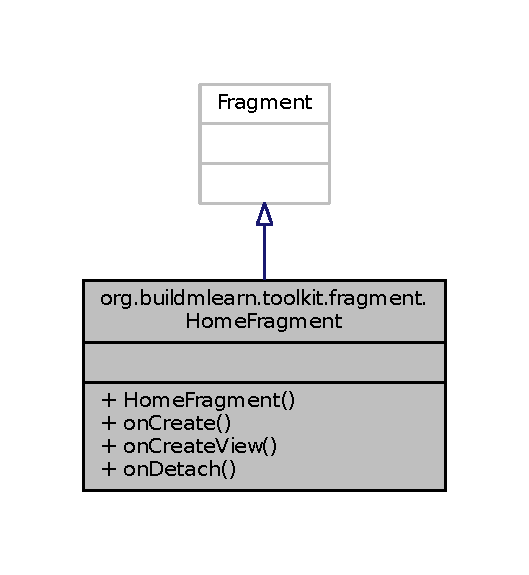
\includegraphics[width=254pt]{da/da2/classorg_1_1buildmlearn_1_1toolkit_1_1fragment_1_1HomeFragment__inherit__graph}
\end{center}
\end{figure}


Collaboration diagram for org.\-buildmlearn.\-toolkit.\-fragment.\-Home\-Fragment\-:
\nopagebreak
\begin{figure}[H]
\begin{center}
\leavevmode
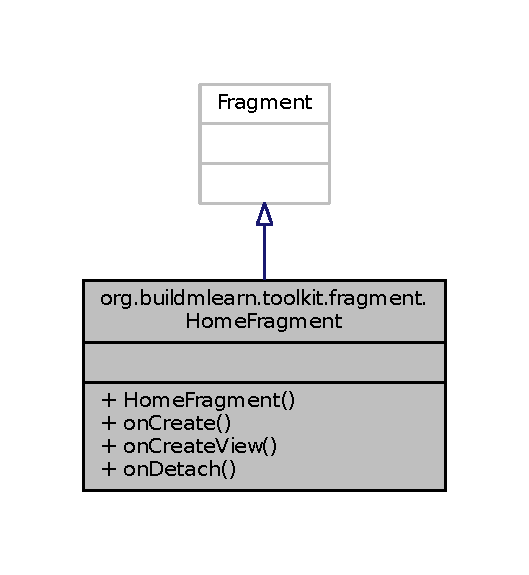
\includegraphics[width=254pt]{d8/d53/classorg_1_1buildmlearn_1_1toolkit_1_1fragment_1_1HomeFragment__coll__graph}
\end{center}
\end{figure}
\subsection*{Public Member Functions}
\begin{DoxyCompactItemize}
\item 
\hyperlink{classorg_1_1buildmlearn_1_1toolkit_1_1fragment_1_1HomeFragment_aa73214b830d5818f31e52a160aefa3e1}{Home\-Fragment} ()
\item 
void \hyperlink{classorg_1_1buildmlearn_1_1toolkit_1_1fragment_1_1HomeFragment_a183d132e866fbc3af61341c95323be94}{on\-Create} (Bundle saved\-Instance\-State)
\item 
View \hyperlink{classorg_1_1buildmlearn_1_1toolkit_1_1fragment_1_1HomeFragment_a80599e92f595260551a0d5753021ebfc}{on\-Create\-View} (Layout\-Inflater inflater, View\-Group container, Bundle saved\-Instance\-State)
\item 
void \hyperlink{classorg_1_1buildmlearn_1_1toolkit_1_1fragment_1_1HomeFragment_a914cfd284407c1daa41b81396c45ef34}{on\-Detach} ()
\end{DoxyCompactItemize}


\subsection{Detailed Description}
Fragment displayed on the home screen. 

\subsection{Constructor \& Destructor Documentation}
\hypertarget{classorg_1_1buildmlearn_1_1toolkit_1_1fragment_1_1HomeFragment_aa73214b830d5818f31e52a160aefa3e1}{\index{org\-::buildmlearn\-::toolkit\-::fragment\-::\-Home\-Fragment@{org\-::buildmlearn\-::toolkit\-::fragment\-::\-Home\-Fragment}!Home\-Fragment@{Home\-Fragment}}
\index{Home\-Fragment@{Home\-Fragment}!org::buildmlearn::toolkit::fragment::HomeFragment@{org\-::buildmlearn\-::toolkit\-::fragment\-::\-Home\-Fragment}}
\subsubsection[{Home\-Fragment}]{\setlength{\rightskip}{0pt plus 5cm}org.\-buildmlearn.\-toolkit.\-fragment.\-Home\-Fragment.\-Home\-Fragment (
\begin{DoxyParamCaption}
{}
\end{DoxyParamCaption}
)}}\label{classorg_1_1buildmlearn_1_1toolkit_1_1fragment_1_1HomeFragment_aa73214b830d5818f31e52a160aefa3e1}

\begin{DoxyCode}
20                           \{
21         \textcolor{comment}{// Required empty public constructor}
22     \}
\end{DoxyCode}


\subsection{Member Function Documentation}
\hypertarget{classorg_1_1buildmlearn_1_1toolkit_1_1fragment_1_1HomeFragment_a183d132e866fbc3af61341c95323be94}{\index{org\-::buildmlearn\-::toolkit\-::fragment\-::\-Home\-Fragment@{org\-::buildmlearn\-::toolkit\-::fragment\-::\-Home\-Fragment}!on\-Create@{on\-Create}}
\index{on\-Create@{on\-Create}!org::buildmlearn::toolkit::fragment::HomeFragment@{org\-::buildmlearn\-::toolkit\-::fragment\-::\-Home\-Fragment}}
\subsubsection[{on\-Create}]{\setlength{\rightskip}{0pt plus 5cm}void org.\-buildmlearn.\-toolkit.\-fragment.\-Home\-Fragment.\-on\-Create (
\begin{DoxyParamCaption}
\item[{Bundle}]{saved\-Instance\-State}
\end{DoxyParamCaption}
)}}\label{classorg_1_1buildmlearn_1_1toolkit_1_1fragment_1_1HomeFragment_a183d132e866fbc3af61341c95323be94}





\begin{DoxyCode}
27                                                     \{
28         super.onCreate(savedInstanceState);
29 
30     \}
\end{DoxyCode}
\hypertarget{classorg_1_1buildmlearn_1_1toolkit_1_1fragment_1_1HomeFragment_a80599e92f595260551a0d5753021ebfc}{\index{org\-::buildmlearn\-::toolkit\-::fragment\-::\-Home\-Fragment@{org\-::buildmlearn\-::toolkit\-::fragment\-::\-Home\-Fragment}!on\-Create\-View@{on\-Create\-View}}
\index{on\-Create\-View@{on\-Create\-View}!org::buildmlearn::toolkit::fragment::HomeFragment@{org\-::buildmlearn\-::toolkit\-::fragment\-::\-Home\-Fragment}}
\subsubsection[{on\-Create\-View}]{\setlength{\rightskip}{0pt plus 5cm}View org.\-buildmlearn.\-toolkit.\-fragment.\-Home\-Fragment.\-on\-Create\-View (
\begin{DoxyParamCaption}
\item[{Layout\-Inflater}]{inflater, }
\item[{View\-Group}]{container, }
\item[{Bundle}]{saved\-Instance\-State}
\end{DoxyParamCaption}
)}}\label{classorg_1_1buildmlearn_1_1toolkit_1_1fragment_1_1HomeFragment_a80599e92f595260551a0d5753021ebfc}

\begin{DoxyCode}
36                                                         \{
37         \textcolor{comment}{// Inflate the layout for this fragment}
38         View view = inflater.inflate(R.layout.fragment\_home, container, \textcolor{keyword}{false});
39         view.findViewById(R.id.button\_template).setOnClickListener(\textcolor{keyword}{new} View.OnClickListener() \{
40             @Override
41             \textcolor{keyword}{public} \textcolor{keywordtype}{void} onClick(View view) \{
42                 startActivity(\textcolor{keyword}{new} Intent(getActivity(), TemplateActivity.class));
43             \}
44         \});
45         \textcolor{keywordflow}{return} view;
46     \}
\end{DoxyCode}
\hypertarget{classorg_1_1buildmlearn_1_1toolkit_1_1fragment_1_1HomeFragment_a914cfd284407c1daa41b81396c45ef34}{\index{org\-::buildmlearn\-::toolkit\-::fragment\-::\-Home\-Fragment@{org\-::buildmlearn\-::toolkit\-::fragment\-::\-Home\-Fragment}!on\-Detach@{on\-Detach}}
\index{on\-Detach@{on\-Detach}!org::buildmlearn::toolkit::fragment::HomeFragment@{org\-::buildmlearn\-::toolkit\-::fragment\-::\-Home\-Fragment}}
\subsubsection[{on\-Detach}]{\setlength{\rightskip}{0pt plus 5cm}void org.\-buildmlearn.\-toolkit.\-fragment.\-Home\-Fragment.\-on\-Detach (
\begin{DoxyParamCaption}
{}
\end{DoxyParamCaption}
)}}\label{classorg_1_1buildmlearn_1_1toolkit_1_1fragment_1_1HomeFragment_a914cfd284407c1daa41b81396c45ef34}

\begin{DoxyCode}
51                            \{
52         super.onDetach();
53     \}
\end{DoxyCode}


The documentation for this class was generated from the following file\-:\begin{DoxyCompactItemize}
\item 
/\-Buildm\-Learn-\/\-Toolkit-\/\-Android/source-\/code/app/src/main/java/org/buildmlearn/toolkit/fragment/\hyperlink{HomeFragment_8java}{Home\-Fragment.\-java}\end{DoxyCompactItemize}

\hypertarget{classorg_1_1buildmlearn_1_1toolkit_1_1templates_1_1InfoAdapter}{\section{org.\-buildmlearn.\-toolkit.\-templates.\-Info\-Adapter Class Reference}
\label{classorg_1_1buildmlearn_1_1toolkit_1_1templates_1_1InfoAdapter}\index{org.\-buildmlearn.\-toolkit.\-templates.\-Info\-Adapter@{org.\-buildmlearn.\-toolkit.\-templates.\-Info\-Adapter}}
}


Adapter for displaying Info Template Editor data.  




Inheritance diagram for org.\-buildmlearn.\-toolkit.\-templates.\-Info\-Adapter\-:
\nopagebreak
\begin{figure}[H]
\begin{center}
\leavevmode
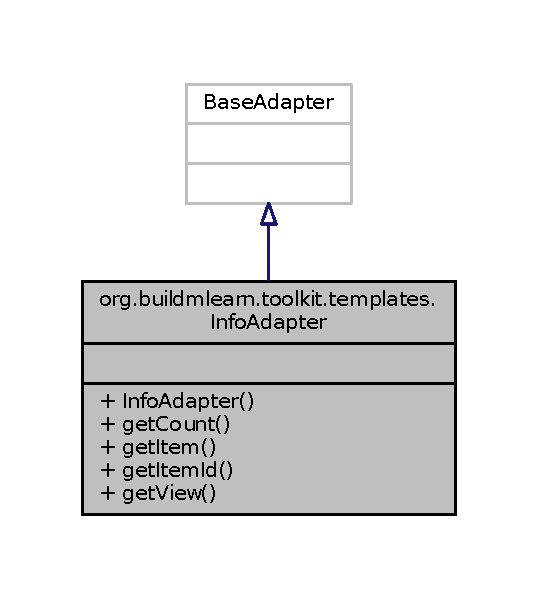
\includegraphics[width=258pt]{d6/d0e/classorg_1_1buildmlearn_1_1toolkit_1_1templates_1_1InfoAdapter__inherit__graph}
\end{center}
\end{figure}


Collaboration diagram for org.\-buildmlearn.\-toolkit.\-templates.\-Info\-Adapter\-:
\nopagebreak
\begin{figure}[H]
\begin{center}
\leavevmode
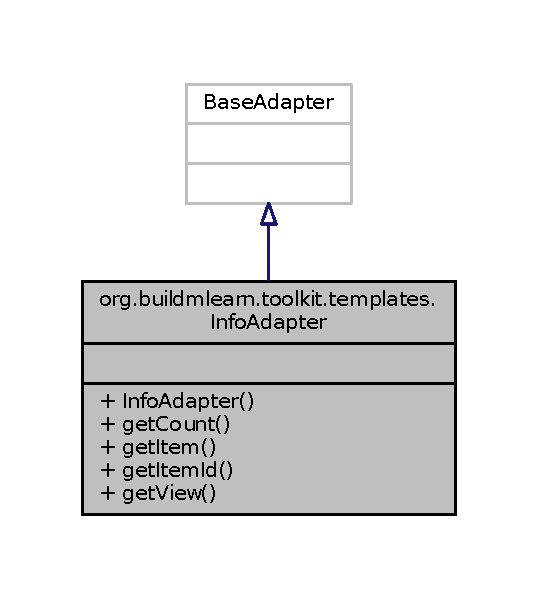
\includegraphics[width=258pt]{d0/dcc/classorg_1_1buildmlearn_1_1toolkit_1_1templates_1_1InfoAdapter__coll__graph}
\end{center}
\end{figure}
\subsection*{Classes}
\begin{DoxyCompactItemize}
\item 
class \hyperlink{classorg_1_1buildmlearn_1_1toolkit_1_1templates_1_1InfoAdapter_1_1InfoTemplateHolder}{Info\-Template\-Holder}
\end{DoxyCompactItemize}
\subsection*{Public Member Functions}
\begin{DoxyCompactItemize}
\item 
\hyperlink{classorg_1_1buildmlearn_1_1toolkit_1_1templates_1_1InfoAdapter_a196fcd7f2757f9e7ede8dd077f23c98e}{Info\-Adapter} (Context m\-Context, Array\-List$<$ \hyperlink{classorg_1_1buildmlearn_1_1toolkit_1_1templates_1_1InfoModel}{Info\-Model} $>$ data)
\item 
int \hyperlink{classorg_1_1buildmlearn_1_1toolkit_1_1templates_1_1InfoAdapter_aea2d9bf9a012c6f483fd86905f84f409}{get\-Count} ()
\item 
\hyperlink{classorg_1_1buildmlearn_1_1toolkit_1_1templates_1_1InfoModel}{Info\-Model} \hyperlink{classorg_1_1buildmlearn_1_1toolkit_1_1templates_1_1InfoAdapter_a12c0148c366d316ed25b8765381eb4d1}{get\-Item} (int position)
\item 
long \hyperlink{classorg_1_1buildmlearn_1_1toolkit_1_1templates_1_1InfoAdapter_ad93b0078702e484916aeb7e670af1d4a}{get\-Item\-Id} (int position)
\item 
View \hyperlink{classorg_1_1buildmlearn_1_1toolkit_1_1templates_1_1InfoAdapter_a78324b9c5e28313fef5e7f4c6ab0f0be}{get\-View} (final int position, View convert\-View, View\-Group parent)
\end{DoxyCompactItemize}


\subsection{Detailed Description}
Adapter for displaying Info Template Editor data. 

Created by abhishek on 17/06/15 at 9\-:48 P\-M. 

\subsection{Constructor \& Destructor Documentation}
\hypertarget{classorg_1_1buildmlearn_1_1toolkit_1_1templates_1_1InfoAdapter_a196fcd7f2757f9e7ede8dd077f23c98e}{\index{org\-::buildmlearn\-::toolkit\-::templates\-::\-Info\-Adapter@{org\-::buildmlearn\-::toolkit\-::templates\-::\-Info\-Adapter}!Info\-Adapter@{Info\-Adapter}}
\index{Info\-Adapter@{Info\-Adapter}!org::buildmlearn::toolkit::templates::InfoAdapter@{org\-::buildmlearn\-::toolkit\-::templates\-::\-Info\-Adapter}}
\subsubsection[{Info\-Adapter}]{\setlength{\rightskip}{0pt plus 5cm}org.\-buildmlearn.\-toolkit.\-templates.\-Info\-Adapter.\-Info\-Adapter (
\begin{DoxyParamCaption}
\item[{Context}]{m\-Context, }
\item[{Array\-List$<$ {\bf Info\-Model} $>$}]{data}
\end{DoxyParamCaption}
)}}\label{classorg_1_1buildmlearn_1_1toolkit_1_1templates_1_1InfoAdapter_a196fcd7f2757f9e7ede8dd077f23c98e}

\begin{DoxyCode}
29                                                                     \{
30         this.mContext = mContext;
31         this.data = data;
32     \}
\end{DoxyCode}


\subsection{Member Function Documentation}
\hypertarget{classorg_1_1buildmlearn_1_1toolkit_1_1templates_1_1InfoAdapter_aea2d9bf9a012c6f483fd86905f84f409}{\index{org\-::buildmlearn\-::toolkit\-::templates\-::\-Info\-Adapter@{org\-::buildmlearn\-::toolkit\-::templates\-::\-Info\-Adapter}!get\-Count@{get\-Count}}
\index{get\-Count@{get\-Count}!org::buildmlearn::toolkit::templates::InfoAdapter@{org\-::buildmlearn\-::toolkit\-::templates\-::\-Info\-Adapter}}
\subsubsection[{get\-Count}]{\setlength{\rightskip}{0pt plus 5cm}int org.\-buildmlearn.\-toolkit.\-templates.\-Info\-Adapter.\-get\-Count (
\begin{DoxyParamCaption}
{}
\end{DoxyParamCaption}
)}}\label{classorg_1_1buildmlearn_1_1toolkit_1_1templates_1_1InfoAdapter_aea2d9bf9a012c6f483fd86905f84f409}

\begin{DoxyCode}
35                           \{
36         \textcolor{keywordflow}{return} data.size();
37     \}
\end{DoxyCode}
\hypertarget{classorg_1_1buildmlearn_1_1toolkit_1_1templates_1_1InfoAdapter_a12c0148c366d316ed25b8765381eb4d1}{\index{org\-::buildmlearn\-::toolkit\-::templates\-::\-Info\-Adapter@{org\-::buildmlearn\-::toolkit\-::templates\-::\-Info\-Adapter}!get\-Item@{get\-Item}}
\index{get\-Item@{get\-Item}!org::buildmlearn::toolkit::templates::InfoAdapter@{org\-::buildmlearn\-::toolkit\-::templates\-::\-Info\-Adapter}}
\subsubsection[{get\-Item}]{\setlength{\rightskip}{0pt plus 5cm}{\bf Info\-Model} org.\-buildmlearn.\-toolkit.\-templates.\-Info\-Adapter.\-get\-Item (
\begin{DoxyParamCaption}
\item[{int}]{position}
\end{DoxyParamCaption}
)}}\label{classorg_1_1buildmlearn_1_1toolkit_1_1templates_1_1InfoAdapter_a12c0148c366d316ed25b8765381eb4d1}

\begin{DoxyCode}
40                                            \{
41         \textcolor{keywordflow}{return} data.get(position);
42     \}
\end{DoxyCode}
\hypertarget{classorg_1_1buildmlearn_1_1toolkit_1_1templates_1_1InfoAdapter_ad93b0078702e484916aeb7e670af1d4a}{\index{org\-::buildmlearn\-::toolkit\-::templates\-::\-Info\-Adapter@{org\-::buildmlearn\-::toolkit\-::templates\-::\-Info\-Adapter}!get\-Item\-Id@{get\-Item\-Id}}
\index{get\-Item\-Id@{get\-Item\-Id}!org::buildmlearn::toolkit::templates::InfoAdapter@{org\-::buildmlearn\-::toolkit\-::templates\-::\-Info\-Adapter}}
\subsubsection[{get\-Item\-Id}]{\setlength{\rightskip}{0pt plus 5cm}long org.\-buildmlearn.\-toolkit.\-templates.\-Info\-Adapter.\-get\-Item\-Id (
\begin{DoxyParamCaption}
\item[{int}]{position}
\end{DoxyParamCaption}
)}}\label{classorg_1_1buildmlearn_1_1toolkit_1_1templates_1_1InfoAdapter_ad93b0078702e484916aeb7e670af1d4a}

\begin{DoxyCode}
45                                         \{
46         \textcolor{keywordflow}{return} position;
47     \}
\end{DoxyCode}
\hypertarget{classorg_1_1buildmlearn_1_1toolkit_1_1templates_1_1InfoAdapter_a78324b9c5e28313fef5e7f4c6ab0f0be}{\index{org\-::buildmlearn\-::toolkit\-::templates\-::\-Info\-Adapter@{org\-::buildmlearn\-::toolkit\-::templates\-::\-Info\-Adapter}!get\-View@{get\-View}}
\index{get\-View@{get\-View}!org::buildmlearn::toolkit::templates::InfoAdapter@{org\-::buildmlearn\-::toolkit\-::templates\-::\-Info\-Adapter}}
\subsubsection[{get\-View}]{\setlength{\rightskip}{0pt plus 5cm}View org.\-buildmlearn.\-toolkit.\-templates.\-Info\-Adapter.\-get\-View (
\begin{DoxyParamCaption}
\item[{final int}]{position, }
\item[{View}]{convert\-View, }
\item[{View\-Group}]{parent}
\end{DoxyParamCaption}
)}}\label{classorg_1_1buildmlearn_1_1toolkit_1_1templates_1_1InfoAdapter_a78324b9c5e28313fef5e7f4c6ab0f0be}

\begin{DoxyCode}
50                                                                                 \{
51 
52         InfoTemplateHolder holder;
53 
54         \textcolor{keywordflow}{if} (convertView == null) \{
55             LayoutInflater inflater = LayoutInflater.from(mContext);
56             convertView = inflater.inflate(R.layout.info\_template\_item, parent, \textcolor{keyword}{false});
57             holder = \textcolor{keyword}{new} InfoTemplateHolder();
58         \} \textcolor{keywordflow}{else} \{
59             holder = (InfoTemplateHolder) convertView.getTag();
60         \}
61 
62         holder.word = (TextViewPlus) convertView.findViewById(R.id.info\_object);
63         holder.meaning = (TextViewPlus) convertView.findViewById(R.id.info\_description);
64 
65         InfoModel info = \hyperlink{classorg_1_1buildmlearn_1_1toolkit_1_1templates_1_1InfoAdapter_a12c0148c366d316ed25b8765381eb4d1}{getItem}(position);
66 
67         holder.meaning.setText(info.getInfoDescription());
68         holder.word.setText(info.getInfoObject());
69         convertView.setTag(holder);
70 
71         holder.deleteButton = (ImageView) convertView.findViewById(R.id.info\_template\_delete);
72         holder.deleteButton.setOnClickListener(\textcolor{keyword}{new} View.OnClickListener() \{
73             @Override
74             \textcolor{keyword}{public} \textcolor{keywordtype}{void} onClick(View v) \{
75 
76                 \textcolor{keyword}{final} MaterialDialog dialog = \textcolor{keyword}{new} MaterialDialog.Builder(mContext)
77                         .title(R.string.info\_template\_delete)
78                         .content(R.string.info\_delete\_item\_content)
79                         .positiveText(R.string.dialog\_yes)
80                         .negativeText(R.string.dialog\_no)
81                         .build();
82 
83                 dialog.getActionButton(DialogAction.POSITIVE).setOnClickListener(\textcolor{keyword}{new} View.OnClickListener()
       \{
84                     @Override
85                     \textcolor{keyword}{public} \textcolor{keywordtype}{void} onClick(View v) \{
86                         data.remove(position);
87                         notifyDataSetChanged();
88                         dialog.dismiss();
89                     \}
90                 \});
91 
92                 dialog.show();
93 
94             \}
95         \});
96 
97         holder.editButton = (ImageView) convertView.findViewById(R.id.info\_template\_edit);
98         holder.editButton.setOnClickListener(\textcolor{keyword}{new} View.OnClickListener() \{
99             @Override
100             \textcolor{keyword}{public} \textcolor{keywordtype}{void} onClick(View v) \{
101                 \textcolor{keyword}{final} MaterialDialog dialog = \textcolor{keyword}{new} MaterialDialog.Builder(mContext)
102                         .title(R.string.info\_add\_new\_title)
103                         .customView(R.layout.info\_dialog\_add\_edit\_data, \textcolor{keyword}{true})
104                         .positiveText(R.string.info\_template\_add)
105                         .negativeText(R.string.info\_template\_delete)
106                         .build();
107 
108                 \textcolor{keyword}{final} InfoModel data = \hyperlink{classorg_1_1buildmlearn_1_1toolkit_1_1templates_1_1InfoAdapter_a12c0148c366d316ed25b8765381eb4d1}{getItem}(position);
109 
110                 \textcolor{keyword}{final} EditText word = (EditText) dialog.findViewById(R.id.info\_word);
111                 \textcolor{keyword}{final} EditText meaning = (EditText) dialog.findViewById(R.id.info\_meaning);
112                 word.setText(data.getInfoObject());
113                 meaning.setText(data.getInfoDescription());
114 
115                 dialog.getActionButton(DialogAction.POSITIVE).setOnClickListener(\textcolor{keyword}{new} View.OnClickListener()
       \{
116                     @Override
117                     \textcolor{keyword}{public} \textcolor{keywordtype}{void} onClick(View v) \{
118 
119                         \textcolor{keywordflow}{if} (InfoTemplate.validated(mContext, word, meaning)) \{
120                             String wordText = word.getText().toString();
121                             String meaningText = meaning.getText().toString();
122 
123                             data.setWord(wordText);
124                             data.setInfoDescription(meaningText);
125 
126                             notifyDataSetChanged();
127                             dialog.dismiss();
128                         \}
129 
130                     \}
131                 \});
132 
133                 dialog.show();
134             \}
135         \});
136 
137 
138         \textcolor{keywordflow}{return} convertView;
139     \}
\end{DoxyCode}


The documentation for this class was generated from the following file\-:\begin{DoxyCompactItemize}
\item 
/\-Buildm\-Learn-\/\-Toolkit-\/\-Android/source-\/code/app/src/main/java/org/buildmlearn/toolkit/templates/\hyperlink{InfoAdapter_8java}{Info\-Adapter.\-java}\end{DoxyCompactItemize}

\hypertarget{classorg_1_1buildmlearn_1_1toolkit_1_1infotemplate_1_1InfoListAdapter}{\section{org.\-buildmlearn.\-toolkit.\-infotemplate.\-Info\-List\-Adapter Class Reference}
\label{classorg_1_1buildmlearn_1_1toolkit_1_1infotemplate_1_1InfoListAdapter}\index{org.\-buildmlearn.\-toolkit.\-infotemplate.\-Info\-List\-Adapter@{org.\-buildmlearn.\-toolkit.\-infotemplate.\-Info\-List\-Adapter}}
}


Simulator code for Info Template.  




Inheritance diagram for org.\-buildmlearn.\-toolkit.\-infotemplate.\-Info\-List\-Adapter\-:
\nopagebreak
\begin{figure}[H]
\begin{center}
\leavevmode
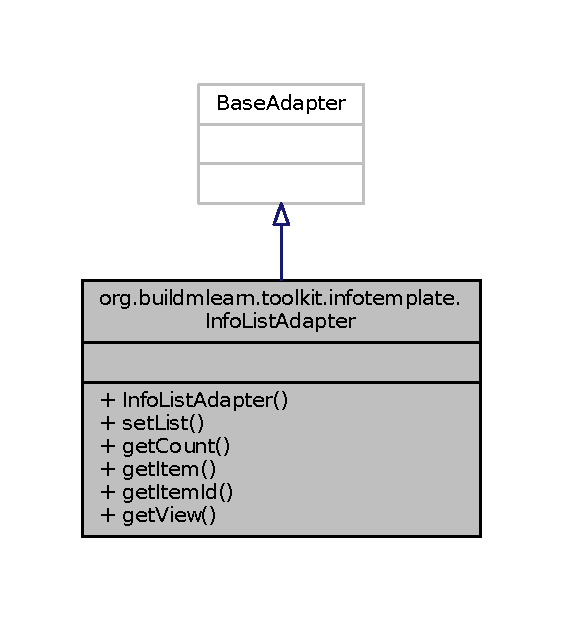
\includegraphics[width=270pt]{d4/d3d/classorg_1_1buildmlearn_1_1toolkit_1_1infotemplate_1_1InfoListAdapter__inherit__graph}
\end{center}
\end{figure}


Collaboration diagram for org.\-buildmlearn.\-toolkit.\-infotemplate.\-Info\-List\-Adapter\-:
\nopagebreak
\begin{figure}[H]
\begin{center}
\leavevmode
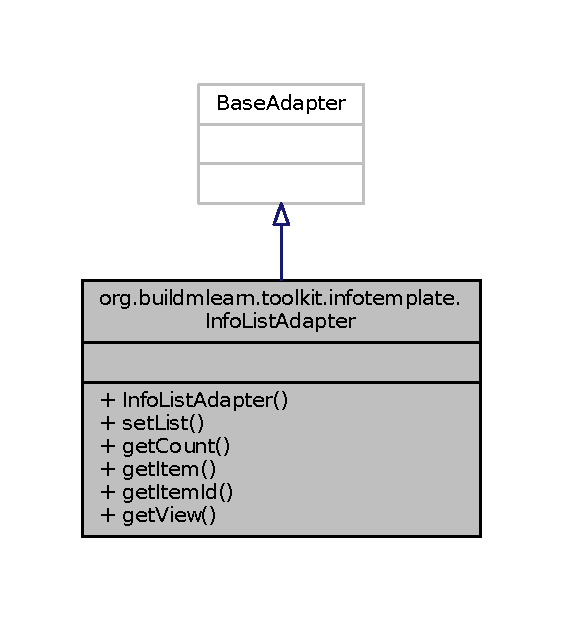
\includegraphics[width=270pt]{dc/d24/classorg_1_1buildmlearn_1_1toolkit_1_1infotemplate_1_1InfoListAdapter__coll__graph}
\end{center}
\end{figure}
\subsection*{Classes}
\begin{DoxyCompactItemize}
\item 
class \hyperlink{classorg_1_1buildmlearn_1_1toolkit_1_1infotemplate_1_1InfoListAdapter_1_1ViewHolder}{View\-Holder}
\end{DoxyCompactItemize}
\subsection*{Public Member Functions}
\begin{DoxyCompactItemize}
\item 
\hyperlink{classorg_1_1buildmlearn_1_1toolkit_1_1infotemplate_1_1InfoListAdapter_a49ce5d5591a6c9a0259400029d9f9e95}{Info\-List\-Adapter} (Context context)
\item 
void \hyperlink{classorg_1_1buildmlearn_1_1toolkit_1_1infotemplate_1_1InfoListAdapter_a4340ea288f1a3992c6bcb81ee26a7ca3}{set\-List} (Array\-List$<$ \hyperlink{classorg_1_1buildmlearn_1_1toolkit_1_1infotemplate_1_1InfoModel}{Info\-Model} $>$ list)
\item 
int \hyperlink{classorg_1_1buildmlearn_1_1toolkit_1_1infotemplate_1_1InfoListAdapter_a24d1690e5fc525192391f448b373adf1}{get\-Count} ()
\item 
Object \hyperlink{classorg_1_1buildmlearn_1_1toolkit_1_1infotemplate_1_1InfoListAdapter_ad2f2a34607cefa59eb5fcbbe950a9e97}{get\-Item} (int position)
\item 
long \hyperlink{classorg_1_1buildmlearn_1_1toolkit_1_1infotemplate_1_1InfoListAdapter_a28df124e7c7e7afcb01cb533b3156567}{get\-Item\-Id} (int position)
\item 
View \hyperlink{classorg_1_1buildmlearn_1_1toolkit_1_1infotemplate_1_1InfoListAdapter_ab16cce97943f53f33bbb5dc9337b756b}{get\-View} (final int position, View convert\-View, View\-Group parent)
\end{DoxyCompactItemize}


\subsection{Detailed Description}
Simulator code for Info Template. 

\subsection{Constructor \& Destructor Documentation}
\hypertarget{classorg_1_1buildmlearn_1_1toolkit_1_1infotemplate_1_1InfoListAdapter_a49ce5d5591a6c9a0259400029d9f9e95}{\index{org\-::buildmlearn\-::toolkit\-::infotemplate\-::\-Info\-List\-Adapter@{org\-::buildmlearn\-::toolkit\-::infotemplate\-::\-Info\-List\-Adapter}!Info\-List\-Adapter@{Info\-List\-Adapter}}
\index{Info\-List\-Adapter@{Info\-List\-Adapter}!org::buildmlearn::toolkit::infotemplate::InfoListAdapter@{org\-::buildmlearn\-::toolkit\-::infotemplate\-::\-Info\-List\-Adapter}}
\subsubsection[{Info\-List\-Adapter}]{\setlength{\rightskip}{0pt plus 5cm}org.\-buildmlearn.\-toolkit.\-infotemplate.\-Info\-List\-Adapter.\-Info\-List\-Adapter (
\begin{DoxyParamCaption}
\item[{Context}]{context}
\end{DoxyParamCaption}
)}}\label{classorg_1_1buildmlearn_1_1toolkit_1_1infotemplate_1_1InfoListAdapter_a49ce5d5591a6c9a0259400029d9f9e95}

\begin{DoxyCode}
22                                             \{
23         mList = \textcolor{keyword}{new} ArrayList<InfoModel>();
24         mContext = context;
25     \}
\end{DoxyCode}


\subsection{Member Function Documentation}
\hypertarget{classorg_1_1buildmlearn_1_1toolkit_1_1infotemplate_1_1InfoListAdapter_a24d1690e5fc525192391f448b373adf1}{\index{org\-::buildmlearn\-::toolkit\-::infotemplate\-::\-Info\-List\-Adapter@{org\-::buildmlearn\-::toolkit\-::infotemplate\-::\-Info\-List\-Adapter}!get\-Count@{get\-Count}}
\index{get\-Count@{get\-Count}!org::buildmlearn::toolkit::infotemplate::InfoListAdapter@{org\-::buildmlearn\-::toolkit\-::infotemplate\-::\-Info\-List\-Adapter}}
\subsubsection[{get\-Count}]{\setlength{\rightskip}{0pt plus 5cm}int org.\-buildmlearn.\-toolkit.\-infotemplate.\-Info\-List\-Adapter.\-get\-Count (
\begin{DoxyParamCaption}
{}
\end{DoxyParamCaption}
)}}\label{classorg_1_1buildmlearn_1_1toolkit_1_1infotemplate_1_1InfoListAdapter_a24d1690e5fc525192391f448b373adf1}

\begin{DoxyCode}
34                           \{
35         \textcolor{keywordflow}{return} mList.size();
36     \}
\end{DoxyCode}
\hypertarget{classorg_1_1buildmlearn_1_1toolkit_1_1infotemplate_1_1InfoListAdapter_ad2f2a34607cefa59eb5fcbbe950a9e97}{\index{org\-::buildmlearn\-::toolkit\-::infotemplate\-::\-Info\-List\-Adapter@{org\-::buildmlearn\-::toolkit\-::infotemplate\-::\-Info\-List\-Adapter}!get\-Item@{get\-Item}}
\index{get\-Item@{get\-Item}!org::buildmlearn::toolkit::infotemplate::InfoListAdapter@{org\-::buildmlearn\-::toolkit\-::infotemplate\-::\-Info\-List\-Adapter}}
\subsubsection[{get\-Item}]{\setlength{\rightskip}{0pt plus 5cm}Object org.\-buildmlearn.\-toolkit.\-infotemplate.\-Info\-List\-Adapter.\-get\-Item (
\begin{DoxyParamCaption}
\item[{int}]{position}
\end{DoxyParamCaption}
)}}\label{classorg_1_1buildmlearn_1_1toolkit_1_1infotemplate_1_1InfoListAdapter_ad2f2a34607cefa59eb5fcbbe950a9e97}

\begin{DoxyCode}
39                                         \{
40         \textcolor{keywordflow}{return} mList.get(position);
41     \}
\end{DoxyCode}
\hypertarget{classorg_1_1buildmlearn_1_1toolkit_1_1infotemplate_1_1InfoListAdapter_a28df124e7c7e7afcb01cb533b3156567}{\index{org\-::buildmlearn\-::toolkit\-::infotemplate\-::\-Info\-List\-Adapter@{org\-::buildmlearn\-::toolkit\-::infotemplate\-::\-Info\-List\-Adapter}!get\-Item\-Id@{get\-Item\-Id}}
\index{get\-Item\-Id@{get\-Item\-Id}!org::buildmlearn::toolkit::infotemplate::InfoListAdapter@{org\-::buildmlearn\-::toolkit\-::infotemplate\-::\-Info\-List\-Adapter}}
\subsubsection[{get\-Item\-Id}]{\setlength{\rightskip}{0pt plus 5cm}long org.\-buildmlearn.\-toolkit.\-infotemplate.\-Info\-List\-Adapter.\-get\-Item\-Id (
\begin{DoxyParamCaption}
\item[{int}]{position}
\end{DoxyParamCaption}
)}}\label{classorg_1_1buildmlearn_1_1toolkit_1_1infotemplate_1_1InfoListAdapter_a28df124e7c7e7afcb01cb533b3156567}

\begin{DoxyCode}
44                                         \{
45         \textcolor{keywordflow}{return} position;
46     \}
\end{DoxyCode}
\hypertarget{classorg_1_1buildmlearn_1_1toolkit_1_1infotemplate_1_1InfoListAdapter_ab16cce97943f53f33bbb5dc9337b756b}{\index{org\-::buildmlearn\-::toolkit\-::infotemplate\-::\-Info\-List\-Adapter@{org\-::buildmlearn\-::toolkit\-::infotemplate\-::\-Info\-List\-Adapter}!get\-View@{get\-View}}
\index{get\-View@{get\-View}!org::buildmlearn::toolkit::infotemplate::InfoListAdapter@{org\-::buildmlearn\-::toolkit\-::infotemplate\-::\-Info\-List\-Adapter}}
\subsubsection[{get\-View}]{\setlength{\rightskip}{0pt plus 5cm}View org.\-buildmlearn.\-toolkit.\-infotemplate.\-Info\-List\-Adapter.\-get\-View (
\begin{DoxyParamCaption}
\item[{final int}]{position, }
\item[{View}]{convert\-View, }
\item[{View\-Group}]{parent}
\end{DoxyParamCaption}
)}}\label{classorg_1_1buildmlearn_1_1toolkit_1_1infotemplate_1_1InfoListAdapter_ab16cce97943f53f33bbb5dc9337b756b}

\begin{DoxyCode}
49                                                                                 \{
50         ViewHolder holder = null;
51         \textcolor{keywordflow}{if} (convertView == null) \{
52 
53             LayoutInflater inflater = LayoutInflater.from(mContext);
54             convertView = inflater.inflate(R.layout.info\_template\_app\_list\_item, parent,
55                     \textcolor{keyword}{false});
56 
57             holder = \textcolor{keyword}{new} ViewHolder();
58             holder.mTvInfoObject = (TextView) convertView
59                     .findViewById(R.id.tv\_info\_object);
60             convertView.setTag(holder);
61 
62         \} \textcolor{keywordflow}{else} \{
63             holder = (ViewHolder) convertView.getTag();
64         \}
65         holder.mTvInfoObject.setTag(R.id.tv\_info\_object);
66         holder.mTvInfoObject.setText(mList.get(position).getInfo\_object());
67 
68         \textcolor{keywordflow}{return} convertView;
69     \}
\end{DoxyCode}
\hypertarget{classorg_1_1buildmlearn_1_1toolkit_1_1infotemplate_1_1InfoListAdapter_a4340ea288f1a3992c6bcb81ee26a7ca3}{\index{org\-::buildmlearn\-::toolkit\-::infotemplate\-::\-Info\-List\-Adapter@{org\-::buildmlearn\-::toolkit\-::infotemplate\-::\-Info\-List\-Adapter}!set\-List@{set\-List}}
\index{set\-List@{set\-List}!org::buildmlearn::toolkit::infotemplate::InfoListAdapter@{org\-::buildmlearn\-::toolkit\-::infotemplate\-::\-Info\-List\-Adapter}}
\subsubsection[{set\-List}]{\setlength{\rightskip}{0pt plus 5cm}void org.\-buildmlearn.\-toolkit.\-infotemplate.\-Info\-List\-Adapter.\-set\-List (
\begin{DoxyParamCaption}
\item[{Array\-List$<$ {\bf Info\-Model} $>$}]{list}
\end{DoxyParamCaption}
)}}\label{classorg_1_1buildmlearn_1_1toolkit_1_1infotemplate_1_1InfoListAdapter_a4340ea288f1a3992c6bcb81ee26a7ca3}

\begin{DoxyCode}
27                                                    \{
28         mList = list;
29         this.notifyDataSetChanged();
30 
31     \}
\end{DoxyCode}


The documentation for this class was generated from the following file\-:\begin{DoxyCompactItemize}
\item 
/\-Buildm\-Learn-\/\-Toolkit-\/\-Android/source-\/code/app/src/main/java/org/buildmlearn/toolkit/infotemplate/\hyperlink{InfoListAdapter_8java}{Info\-List\-Adapter.\-java}\end{DoxyCompactItemize}

\hypertarget{classorg_1_1buildmlearn_1_1toolkit_1_1infotemplate_1_1InfoModel}{\section{org.\-buildmlearn.\-toolkit.\-infotemplate.\-Info\-Model Class Reference}
\label{classorg_1_1buildmlearn_1_1toolkit_1_1infotemplate_1_1InfoModel}\index{org.\-buildmlearn.\-toolkit.\-infotemplate.\-Info\-Model@{org.\-buildmlearn.\-toolkit.\-infotemplate.\-Info\-Model}}
}


Simulator code for Info Template.  




Collaboration diagram for org.\-buildmlearn.\-toolkit.\-infotemplate.\-Info\-Model\-:
\nopagebreak
\begin{figure}[H]
\begin{center}
\leavevmode
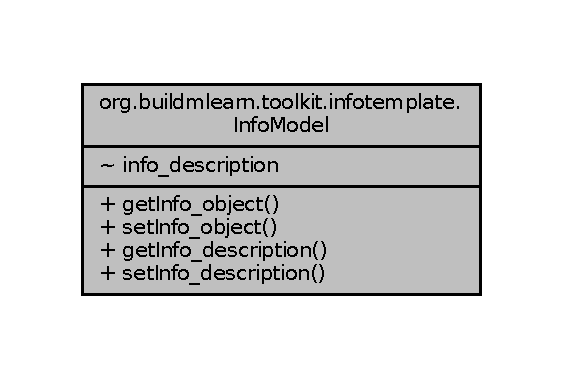
\includegraphics[width=270pt]{d3/dbc/classorg_1_1buildmlearn_1_1toolkit_1_1infotemplate_1_1InfoModel__coll__graph}
\end{center}
\end{figure}
\subsection*{Public Member Functions}
\begin{DoxyCompactItemize}
\item 
String \hyperlink{classorg_1_1buildmlearn_1_1toolkit_1_1infotemplate_1_1InfoModel_aa1f40de4a1f2b4eecdb69f4a449b015b}{get\-Info\-\_\-object} ()
\item 
void \hyperlink{classorg_1_1buildmlearn_1_1toolkit_1_1infotemplate_1_1InfoModel_a028f6fa4a7e5abc3ca2aa99cda4b59cd}{set\-Info\-\_\-object} (String info\-\_\-object)
\item 
String \hyperlink{classorg_1_1buildmlearn_1_1toolkit_1_1infotemplate_1_1InfoModel_a2f0005dd0a926471dbaa2c92e459d0df}{get\-Info\-\_\-description} ()
\item 
void \hyperlink{classorg_1_1buildmlearn_1_1toolkit_1_1infotemplate_1_1InfoModel_a983bb06e7e3f4d477d1059321981c5b3}{set\-Info\-\_\-description} (String info\-\_\-description)
\end{DoxyCompactItemize}


\subsection{Detailed Description}
Simulator code for Info Template. 

\subsection{Member Function Documentation}
\hypertarget{classorg_1_1buildmlearn_1_1toolkit_1_1infotemplate_1_1InfoModel_a2f0005dd0a926471dbaa2c92e459d0df}{\index{org\-::buildmlearn\-::toolkit\-::infotemplate\-::\-Info\-Model@{org\-::buildmlearn\-::toolkit\-::infotemplate\-::\-Info\-Model}!get\-Info\-\_\-description@{get\-Info\-\_\-description}}
\index{get\-Info\-\_\-description@{get\-Info\-\_\-description}!org::buildmlearn::toolkit::infotemplate::InfoModel@{org\-::buildmlearn\-::toolkit\-::infotemplate\-::\-Info\-Model}}
\subsubsection[{get\-Info\-\_\-description}]{\setlength{\rightskip}{0pt plus 5cm}String org.\-buildmlearn.\-toolkit.\-infotemplate.\-Info\-Model.\-get\-Info\-\_\-description (
\begin{DoxyParamCaption}
{}
\end{DoxyParamCaption}
)}}\label{classorg_1_1buildmlearn_1_1toolkit_1_1infotemplate_1_1InfoModel_a2f0005dd0a926471dbaa2c92e459d0df}

\begin{DoxyCode}
18                                         \{
19         \textcolor{keywordflow}{return} info\_description;
20     \}
\end{DoxyCode}
\hypertarget{classorg_1_1buildmlearn_1_1toolkit_1_1infotemplate_1_1InfoModel_aa1f40de4a1f2b4eecdb69f4a449b015b}{\index{org\-::buildmlearn\-::toolkit\-::infotemplate\-::\-Info\-Model@{org\-::buildmlearn\-::toolkit\-::infotemplate\-::\-Info\-Model}!get\-Info\-\_\-object@{get\-Info\-\_\-object}}
\index{get\-Info\-\_\-object@{get\-Info\-\_\-object}!org::buildmlearn::toolkit::infotemplate::InfoModel@{org\-::buildmlearn\-::toolkit\-::infotemplate\-::\-Info\-Model}}
\subsubsection[{get\-Info\-\_\-object}]{\setlength{\rightskip}{0pt plus 5cm}String org.\-buildmlearn.\-toolkit.\-infotemplate.\-Info\-Model.\-get\-Info\-\_\-object (
\begin{DoxyParamCaption}
{}
\end{DoxyParamCaption}
)}}\label{classorg_1_1buildmlearn_1_1toolkit_1_1infotemplate_1_1InfoModel_aa1f40de4a1f2b4eecdb69f4a449b015b}

\begin{DoxyCode}
10                                    \{
11         \textcolor{keywordflow}{return} info\_object;
12     \}
\end{DoxyCode}
\hypertarget{classorg_1_1buildmlearn_1_1toolkit_1_1infotemplate_1_1InfoModel_a983bb06e7e3f4d477d1059321981c5b3}{\index{org\-::buildmlearn\-::toolkit\-::infotemplate\-::\-Info\-Model@{org\-::buildmlearn\-::toolkit\-::infotemplate\-::\-Info\-Model}!set\-Info\-\_\-description@{set\-Info\-\_\-description}}
\index{set\-Info\-\_\-description@{set\-Info\-\_\-description}!org::buildmlearn::toolkit::infotemplate::InfoModel@{org\-::buildmlearn\-::toolkit\-::infotemplate\-::\-Info\-Model}}
\subsubsection[{set\-Info\-\_\-description}]{\setlength{\rightskip}{0pt plus 5cm}void org.\-buildmlearn.\-toolkit.\-infotemplate.\-Info\-Model.\-set\-Info\-\_\-description (
\begin{DoxyParamCaption}
\item[{String}]{info\-\_\-description}
\end{DoxyParamCaption}
)}}\label{classorg_1_1buildmlearn_1_1toolkit_1_1infotemplate_1_1InfoModel_a983bb06e7e3f4d477d1059321981c5b3}

\begin{DoxyCode}
22                                                              \{
23         this.info\_description = info\_description;
24     \}
\end{DoxyCode}
\hypertarget{classorg_1_1buildmlearn_1_1toolkit_1_1infotemplate_1_1InfoModel_a028f6fa4a7e5abc3ca2aa99cda4b59cd}{\index{org\-::buildmlearn\-::toolkit\-::infotemplate\-::\-Info\-Model@{org\-::buildmlearn\-::toolkit\-::infotemplate\-::\-Info\-Model}!set\-Info\-\_\-object@{set\-Info\-\_\-object}}
\index{set\-Info\-\_\-object@{set\-Info\-\_\-object}!org::buildmlearn::toolkit::infotemplate::InfoModel@{org\-::buildmlearn\-::toolkit\-::infotemplate\-::\-Info\-Model}}
\subsubsection[{set\-Info\-\_\-object}]{\setlength{\rightskip}{0pt plus 5cm}void org.\-buildmlearn.\-toolkit.\-infotemplate.\-Info\-Model.\-set\-Info\-\_\-object (
\begin{DoxyParamCaption}
\item[{String}]{info\-\_\-object}
\end{DoxyParamCaption}
)}}\label{classorg_1_1buildmlearn_1_1toolkit_1_1infotemplate_1_1InfoModel_a028f6fa4a7e5abc3ca2aa99cda4b59cd}

\begin{DoxyCode}
14                                                    \{
15         this.info\_object = info\_object;
16     \}
\end{DoxyCode}


The documentation for this class was generated from the following file\-:\begin{DoxyCompactItemize}
\item 
/\-Buildm\-Learn-\/\-Toolkit-\/\-Android/source-\/code/app/src/main/java/org/buildmlearn/toolkit/infotemplate/\hyperlink{infotemplate_2InfoModel_8java}{Info\-Model.\-java}\end{DoxyCompactItemize}

\hypertarget{classorg_1_1buildmlearn_1_1toolkit_1_1templates_1_1InfoModel}{\section{org.\-buildmlearn.\-toolkit.\-templates.\-Info\-Model Class Reference}
\label{classorg_1_1buildmlearn_1_1toolkit_1_1templates_1_1InfoModel}\index{org.\-buildmlearn.\-toolkit.\-templates.\-Info\-Model@{org.\-buildmlearn.\-toolkit.\-templates.\-Info\-Model}}
}


Model class for Info Template Editor data.  




Inheritance diagram for org.\-buildmlearn.\-toolkit.\-templates.\-Info\-Model\-:
\nopagebreak
\begin{figure}[H]
\begin{center}
\leavevmode
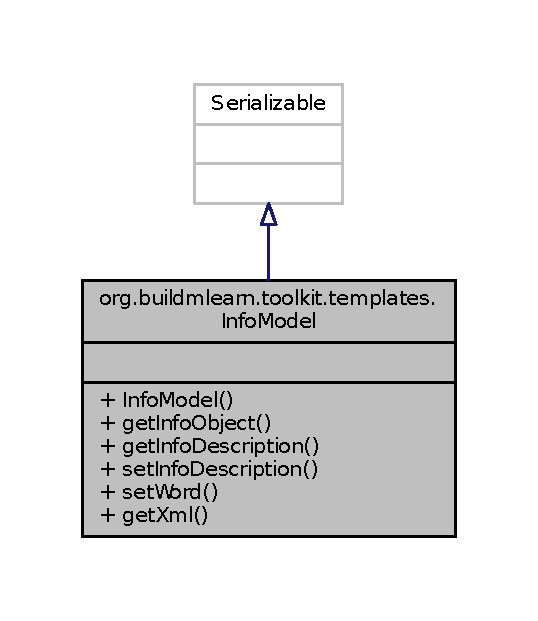
\includegraphics[width=258pt]{dd/dce/classorg_1_1buildmlearn_1_1toolkit_1_1templates_1_1InfoModel__inherit__graph}
\end{center}
\end{figure}


Collaboration diagram for org.\-buildmlearn.\-toolkit.\-templates.\-Info\-Model\-:
\nopagebreak
\begin{figure}[H]
\begin{center}
\leavevmode
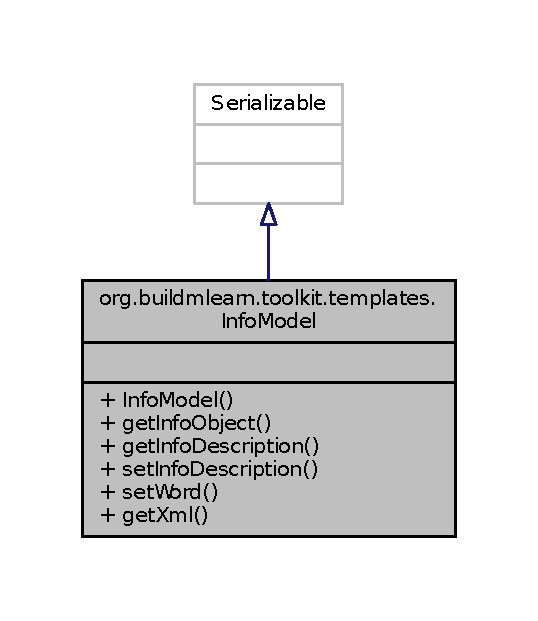
\includegraphics[width=258pt]{dc/d37/classorg_1_1buildmlearn_1_1toolkit_1_1templates_1_1InfoModel__coll__graph}
\end{center}
\end{figure}
\subsection*{Public Member Functions}
\begin{DoxyCompactItemize}
\item 
\hyperlink{classorg_1_1buildmlearn_1_1toolkit_1_1templates_1_1InfoModel_a5ffb5146ce8fcf0e4504cd8870e26544}{Info\-Model} (String info\-Object, String meaning)
\item 
String \hyperlink{classorg_1_1buildmlearn_1_1toolkit_1_1templates_1_1InfoModel_a34b917e09a5b8a369d9a1b8fdb4e1043}{get\-Info\-Object} ()
\item 
String \hyperlink{classorg_1_1buildmlearn_1_1toolkit_1_1templates_1_1InfoModel_aaa53a79383392b5be51d202b76e65c5f}{get\-Info\-Description} ()
\item 
void \hyperlink{classorg_1_1buildmlearn_1_1toolkit_1_1templates_1_1InfoModel_a80956d6760064ebac06c98b0cd748825}{set\-Info\-Description} (String info\-Description)
\item 
void \hyperlink{classorg_1_1buildmlearn_1_1toolkit_1_1templates_1_1InfoModel_a207189ef74d5c4f2fc4a356d6135c14e}{set\-Word} (String word)
\item 
Element \hyperlink{classorg_1_1buildmlearn_1_1toolkit_1_1templates_1_1InfoModel_a603a8ab258eec5da500824267cbb86df}{get\-Xml} (Document doc)
\end{DoxyCompactItemize}


\subsection{Detailed Description}
Model class for Info Template Editor data. 

Created by abhishek on 17/06/15 at 9\-:49 P\-M. 

\subsection{Constructor \& Destructor Documentation}
\hypertarget{classorg_1_1buildmlearn_1_1toolkit_1_1templates_1_1InfoModel_a5ffb5146ce8fcf0e4504cd8870e26544}{\index{org\-::buildmlearn\-::toolkit\-::templates\-::\-Info\-Model@{org\-::buildmlearn\-::toolkit\-::templates\-::\-Info\-Model}!Info\-Model@{Info\-Model}}
\index{Info\-Model@{Info\-Model}!org::buildmlearn::toolkit::templates::InfoModel@{org\-::buildmlearn\-::toolkit\-::templates\-::\-Info\-Model}}
\subsubsection[{Info\-Model}]{\setlength{\rightskip}{0pt plus 5cm}org.\-buildmlearn.\-toolkit.\-templates.\-Info\-Model.\-Info\-Model (
\begin{DoxyParamCaption}
\item[{String}]{info\-Object, }
\item[{String}]{meaning}
\end{DoxyParamCaption}
)}}\label{classorg_1_1buildmlearn_1_1toolkit_1_1templates_1_1InfoModel_a5ffb5146ce8fcf0e4504cd8870e26544}

\begin{DoxyCode}
18                                                         \{
19         this.infoObject = infoObject;
20         this.infoDescription = meaning;
21     \}
\end{DoxyCode}


\subsection{Member Function Documentation}
\hypertarget{classorg_1_1buildmlearn_1_1toolkit_1_1templates_1_1InfoModel_aaa53a79383392b5be51d202b76e65c5f}{\index{org\-::buildmlearn\-::toolkit\-::templates\-::\-Info\-Model@{org\-::buildmlearn\-::toolkit\-::templates\-::\-Info\-Model}!get\-Info\-Description@{get\-Info\-Description}}
\index{get\-Info\-Description@{get\-Info\-Description}!org::buildmlearn::toolkit::templates::InfoModel@{org\-::buildmlearn\-::toolkit\-::templates\-::\-Info\-Model}}
\subsubsection[{get\-Info\-Description}]{\setlength{\rightskip}{0pt plus 5cm}String org.\-buildmlearn.\-toolkit.\-templates.\-Info\-Model.\-get\-Info\-Description (
\begin{DoxyParamCaption}
{}
\end{DoxyParamCaption}
)}}\label{classorg_1_1buildmlearn_1_1toolkit_1_1templates_1_1InfoModel_aaa53a79383392b5be51d202b76e65c5f}

\begin{DoxyCode}
27                                        \{
28         \textcolor{keywordflow}{return} infoDescription;
29     \}
\end{DoxyCode}
\hypertarget{classorg_1_1buildmlearn_1_1toolkit_1_1templates_1_1InfoModel_a34b917e09a5b8a369d9a1b8fdb4e1043}{\index{org\-::buildmlearn\-::toolkit\-::templates\-::\-Info\-Model@{org\-::buildmlearn\-::toolkit\-::templates\-::\-Info\-Model}!get\-Info\-Object@{get\-Info\-Object}}
\index{get\-Info\-Object@{get\-Info\-Object}!org::buildmlearn::toolkit::templates::InfoModel@{org\-::buildmlearn\-::toolkit\-::templates\-::\-Info\-Model}}
\subsubsection[{get\-Info\-Object}]{\setlength{\rightskip}{0pt plus 5cm}String org.\-buildmlearn.\-toolkit.\-templates.\-Info\-Model.\-get\-Info\-Object (
\begin{DoxyParamCaption}
{}
\end{DoxyParamCaption}
)}}\label{classorg_1_1buildmlearn_1_1toolkit_1_1templates_1_1InfoModel_a34b917e09a5b8a369d9a1b8fdb4e1043}

\begin{DoxyCode}
23                                   \{
24         \textcolor{keywordflow}{return} infoObject;
25     \}
\end{DoxyCode}
\hypertarget{classorg_1_1buildmlearn_1_1toolkit_1_1templates_1_1InfoModel_a603a8ab258eec5da500824267cbb86df}{\index{org\-::buildmlearn\-::toolkit\-::templates\-::\-Info\-Model@{org\-::buildmlearn\-::toolkit\-::templates\-::\-Info\-Model}!get\-Xml@{get\-Xml}}
\index{get\-Xml@{get\-Xml}!org::buildmlearn::toolkit::templates::InfoModel@{org\-::buildmlearn\-::toolkit\-::templates\-::\-Info\-Model}}
\subsubsection[{get\-Xml}]{\setlength{\rightskip}{0pt plus 5cm}Element org.\-buildmlearn.\-toolkit.\-templates.\-Info\-Model.\-get\-Xml (
\begin{DoxyParamCaption}
\item[{Document}]{doc}
\end{DoxyParamCaption}
)}}\label{classorg_1_1buildmlearn_1_1toolkit_1_1templates_1_1InfoModel_a603a8ab258eec5da500824267cbb86df}

\begin{DoxyCode}
39                                         \{
40         Element rootElement = doc.createElement(\textcolor{stringliteral}{"item"});
41         Element questionElement = doc.createElement(\textcolor{stringliteral}{"item\_title"});
42         questionElement.appendChild(doc.createTextNode(infoObject));
43         rootElement.appendChild(questionElement);
44         Element answerElement = doc.createElement(\textcolor{stringliteral}{"item\_description"});
45         answerElement.appendChild(doc.createTextNode(String.valueOf(infoDescription)));
46         rootElement.appendChild(answerElement);
47         \textcolor{keywordflow}{return} rootElement;
48     \}
\end{DoxyCode}
\hypertarget{classorg_1_1buildmlearn_1_1toolkit_1_1templates_1_1InfoModel_a80956d6760064ebac06c98b0cd748825}{\index{org\-::buildmlearn\-::toolkit\-::templates\-::\-Info\-Model@{org\-::buildmlearn\-::toolkit\-::templates\-::\-Info\-Model}!set\-Info\-Description@{set\-Info\-Description}}
\index{set\-Info\-Description@{set\-Info\-Description}!org::buildmlearn::toolkit::templates::InfoModel@{org\-::buildmlearn\-::toolkit\-::templates\-::\-Info\-Model}}
\subsubsection[{set\-Info\-Description}]{\setlength{\rightskip}{0pt plus 5cm}void org.\-buildmlearn.\-toolkit.\-templates.\-Info\-Model.\-set\-Info\-Description (
\begin{DoxyParamCaption}
\item[{String}]{info\-Description}
\end{DoxyParamCaption}
)}}\label{classorg_1_1buildmlearn_1_1toolkit_1_1templates_1_1InfoModel_a80956d6760064ebac06c98b0cd748825}

\begin{DoxyCode}
31                                                            \{
32         this.infoDescription = infoDescription;
33     \}
\end{DoxyCode}
\hypertarget{classorg_1_1buildmlearn_1_1toolkit_1_1templates_1_1InfoModel_a207189ef74d5c4f2fc4a356d6135c14e}{\index{org\-::buildmlearn\-::toolkit\-::templates\-::\-Info\-Model@{org\-::buildmlearn\-::toolkit\-::templates\-::\-Info\-Model}!set\-Word@{set\-Word}}
\index{set\-Word@{set\-Word}!org::buildmlearn::toolkit::templates::InfoModel@{org\-::buildmlearn\-::toolkit\-::templates\-::\-Info\-Model}}
\subsubsection[{set\-Word}]{\setlength{\rightskip}{0pt plus 5cm}void org.\-buildmlearn.\-toolkit.\-templates.\-Info\-Model.\-set\-Word (
\begin{DoxyParamCaption}
\item[{String}]{word}
\end{DoxyParamCaption}
)}}\label{classorg_1_1buildmlearn_1_1toolkit_1_1templates_1_1InfoModel_a207189ef74d5c4f2fc4a356d6135c14e}

\begin{DoxyCode}
35                                      \{
36         this.infoObject = word;
37     \}
\end{DoxyCode}


The documentation for this class was generated from the following file\-:\begin{DoxyCompactItemize}
\item 
/\-Buildm\-Learn-\/\-Toolkit-\/\-Android/source-\/code/app/src/main/java/org/buildmlearn/toolkit/templates/\hyperlink{templates_2InfoModel_8java}{Info\-Model.\-java}\end{DoxyCompactItemize}

\hypertarget{classorg_1_1buildmlearn_1_1toolkit_1_1templates_1_1InfoTemplate}{\section{org.\-buildmlearn.\-toolkit.\-templates.\-Info\-Template Class Reference}
\label{classorg_1_1buildmlearn_1_1toolkit_1_1templates_1_1InfoTemplate}\index{org.\-buildmlearn.\-toolkit.\-templates.\-Info\-Template@{org.\-buildmlearn.\-toolkit.\-templates.\-Info\-Template}}
}


Info template code implementing methods of Template\-Interface.  




Inheritance diagram for org.\-buildmlearn.\-toolkit.\-templates.\-Info\-Template\-:
\nopagebreak
\begin{figure}[H]
\begin{center}
\leavevmode
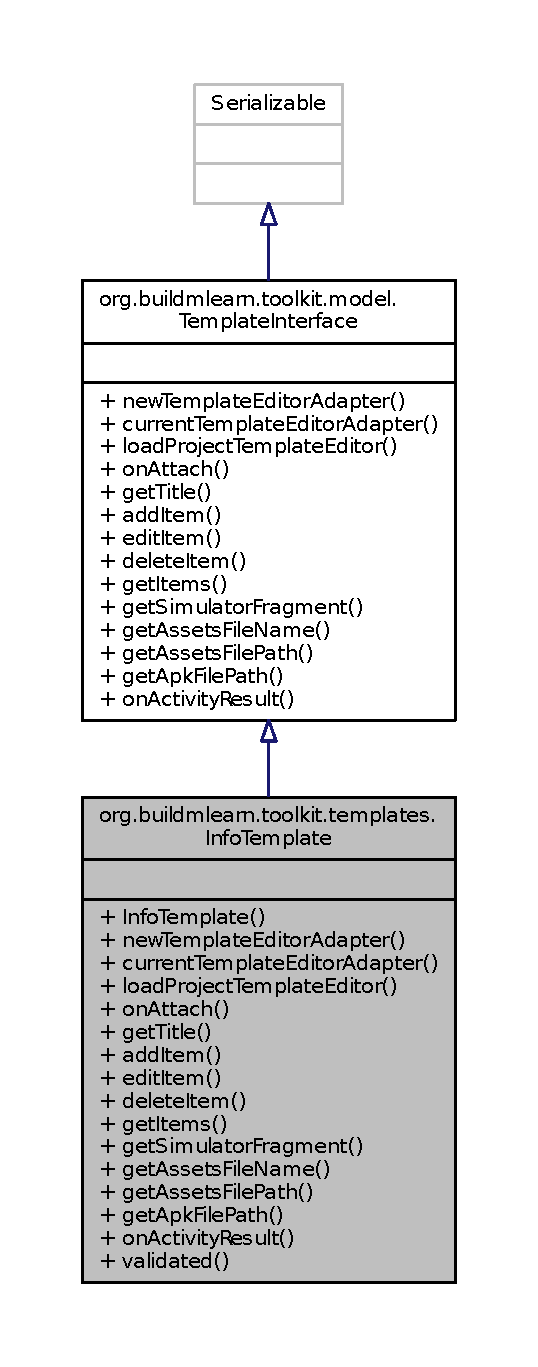
\includegraphics[height=550pt]{d2/d3d/classorg_1_1buildmlearn_1_1toolkit_1_1templates_1_1InfoTemplate__inherit__graph}
\end{center}
\end{figure}


Collaboration diagram for org.\-buildmlearn.\-toolkit.\-templates.\-Info\-Template\-:
\nopagebreak
\begin{figure}[H]
\begin{center}
\leavevmode
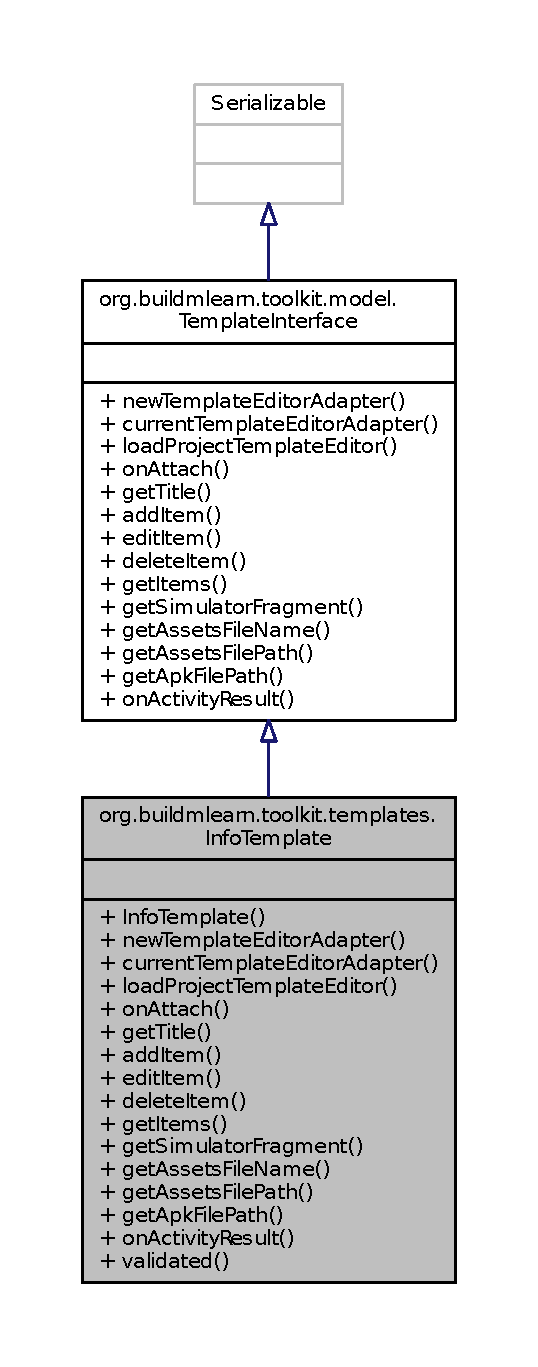
\includegraphics[height=550pt]{d7/dfb/classorg_1_1buildmlearn_1_1toolkit_1_1templates_1_1InfoTemplate__coll__graph}
\end{center}
\end{figure}
\subsection*{Public Member Functions}
\begin{DoxyCompactItemize}
\item 
\hyperlink{classorg_1_1buildmlearn_1_1toolkit_1_1templates_1_1InfoTemplate_a3f9f925728b785f52105776cf4ba0e44}{Info\-Template} ()
\item 
Base\-Adapter \hyperlink{classorg_1_1buildmlearn_1_1toolkit_1_1templates_1_1InfoTemplate_ab4d81e3a7da28f406ca3b6e8c74bb69c}{new\-Template\-Editor\-Adapter} (Context context)
\begin{DoxyCompactList}\small\item\em Called from Template Editor when template editor is started for creating a new template project. \end{DoxyCompactList}\item 
Base\-Adapter \hyperlink{classorg_1_1buildmlearn_1_1toolkit_1_1templates_1_1InfoTemplate_adf457576e88abf2859b9d8cfb8097eba}{current\-Template\-Editor\-Adapter} ()
\begin{DoxyCompactList}\small\item\em This function is used to get the adapter (containing template data) for a existing/current template project. \end{DoxyCompactList}\item 
Base\-Adapter \hyperlink{classorg_1_1buildmlearn_1_1toolkit_1_1templates_1_1InfoTemplate_a3133856410f82ddd51ebd42f54a56cf6}{load\-Project\-Template\-Editor} (Context context, Array\-List$<$ Element $>$ data)
\item 
String \hyperlink{classorg_1_1buildmlearn_1_1toolkit_1_1templates_1_1InfoTemplate_ada0d67fc9e941bb29703a19467216a92}{on\-Attach} ()
\begin{DoxyCompactList}\small\item\em Called from Template\-Editor whenever a template is attached to Template\-Editor. \end{DoxyCompactList}\item 
String \hyperlink{classorg_1_1buildmlearn_1_1toolkit_1_1templates_1_1InfoTemplate_aeff54c9ca6a2925582e01d6fffea0b71}{get\-Title} ()
\begin{DoxyCompactList}\small\item\em Used to get the title of the templaye. Mainly used to update Action\-Bar in Template Editor. \end{DoxyCompactList}\item 
void \hyperlink{classorg_1_1buildmlearn_1_1toolkit_1_1templates_1_1InfoTemplate_a397a72ab6a84e7352e8e2af283a9b4a8}{add\-Item} (final Activity activity)
\item 
void \hyperlink{classorg_1_1buildmlearn_1_1toolkit_1_1templates_1_1InfoTemplate_a959e9afa2bb71e903b575087515611a7}{edit\-Item} (final Activity activity, int position)
\item 
void \hyperlink{classorg_1_1buildmlearn_1_1toolkit_1_1templates_1_1InfoTemplate_abcd4da5c42fd2601f72ddbe695a123a9}{delete\-Item} (int position)
\begin{DoxyCompactList}\small\item\em Remove an item form template data list. \end{DoxyCompactList}\item 
Array\-List$<$ Element $>$ \hyperlink{classorg_1_1buildmlearn_1_1toolkit_1_1templates_1_1InfoTemplate_a720895732bb2e94b7d0a119d7a6b0a6c}{get\-Items} (Document doc)
\item 
Fragment \hyperlink{classorg_1_1buildmlearn_1_1toolkit_1_1templates_1_1InfoTemplate_ad67fb90b9a49c5ae17771252cd722ce0}{get\-Simulator\-Fragment} (String file\-Path\-With\-Name)
\begin{DoxyCompactList}\small\item\em Returns a fragment required for the Simulator Activity. \end{DoxyCompactList}\item 
String \hyperlink{classorg_1_1buildmlearn_1_1toolkit_1_1templates_1_1InfoTemplate_aa2cab0b4c1dabf029612ebebbe8c43af}{get\-Assets\-File\-Name} ()
\begin{DoxyCompactList}\small\item\em Name of the xml file congaing template data in the assets folders in the build apk. \end{DoxyCompactList}\item 
String \hyperlink{classorg_1_1buildmlearn_1_1toolkit_1_1templates_1_1InfoTemplate_a7d33c2515392865627720469c30726cc}{get\-Assets\-File\-Path} ()
\begin{DoxyCompactList}\small\item\em Folder path in which the apk is stored in the build A\-P\-K. \end{DoxyCompactList}\item 
String \hyperlink{classorg_1_1buildmlearn_1_1toolkit_1_1templates_1_1InfoTemplate_a2c1e9f1197aa092e46015da0ed060b6b}{get\-Apk\-File\-Path} ()
\item 
void \hyperlink{classorg_1_1buildmlearn_1_1toolkit_1_1templates_1_1InfoTemplate_a8089c34bead9e0dc798d5e14608e64fd}{on\-Activity\-Result} (Context context, int request\-Code, int result\-Code, Intent intent)
\begin{DoxyCompactList}\small\item\em Called whenever on\-Activity\-Result is called in Template Editor. Can be used to perform action related to intent and callbacks. \end{DoxyCompactList}\end{DoxyCompactItemize}
\subsection*{Static Public Member Functions}
\begin{DoxyCompactItemize}
\item 
static boolean \hyperlink{classorg_1_1buildmlearn_1_1toolkit_1_1templates_1_1InfoTemplate_a6b8cc6c46170f7d0be6be09093f58e41}{validated} (Context context, Edit\-Text word, Edit\-Text meaning)
\end{DoxyCompactItemize}


\subsection{Detailed Description}
Info template code implementing methods of Template\-Interface. 

Created by abhishek on 16/06/15 at 9\-:59 P\-M. 

\subsection{Constructor \& Destructor Documentation}
\hypertarget{classorg_1_1buildmlearn_1_1toolkit_1_1templates_1_1InfoTemplate_a3f9f925728b785f52105776cf4ba0e44}{\index{org\-::buildmlearn\-::toolkit\-::templates\-::\-Info\-Template@{org\-::buildmlearn\-::toolkit\-::templates\-::\-Info\-Template}!Info\-Template@{Info\-Template}}
\index{Info\-Template@{Info\-Template}!org::buildmlearn::toolkit::templates::InfoTemplate@{org\-::buildmlearn\-::toolkit\-::templates\-::\-Info\-Template}}
\subsubsection[{Info\-Template}]{\setlength{\rightskip}{0pt plus 5cm}org.\-buildmlearn.\-toolkit.\-templates.\-Info\-Template.\-Info\-Template (
\begin{DoxyParamCaption}
{}
\end{DoxyParamCaption}
)}}\label{classorg_1_1buildmlearn_1_1toolkit_1_1templates_1_1InfoTemplate_a3f9f925728b785f52105776cf4ba0e44}

\begin{DoxyCode}
33                           \{
34         infoData = \textcolor{keyword}{new} ArrayList<>();
35     \}
\end{DoxyCode}


\subsection{Member Function Documentation}
\hypertarget{classorg_1_1buildmlearn_1_1toolkit_1_1templates_1_1InfoTemplate_a397a72ab6a84e7352e8e2af283a9b4a8}{\index{org\-::buildmlearn\-::toolkit\-::templates\-::\-Info\-Template@{org\-::buildmlearn\-::toolkit\-::templates\-::\-Info\-Template}!add\-Item@{add\-Item}}
\index{add\-Item@{add\-Item}!org::buildmlearn::toolkit::templates::InfoTemplate@{org\-::buildmlearn\-::toolkit\-::templates\-::\-Info\-Template}}
\subsubsection[{add\-Item}]{\setlength{\rightskip}{0pt plus 5cm}void org.\-buildmlearn.\-toolkit.\-templates.\-Info\-Template.\-add\-Item (
\begin{DoxyParamCaption}
\item[{final Activity}]{activity}
\end{DoxyParamCaption}
)}}\label{classorg_1_1buildmlearn_1_1toolkit_1_1templates_1_1InfoTemplate_a397a72ab6a84e7352e8e2af283a9b4a8}

\begin{DoxyCode}
90                                                  \{
91 
92         \textcolor{keyword}{final} MaterialDialog dialog = \textcolor{keyword}{new} MaterialDialog.Builder(activity)
93                 .title(R.string.info\_add\_new\_title)
94                 .customView(R.layout.info\_dialog\_add\_edit\_data, \textcolor{keyword}{true})
95                 .positiveText(R.string.info\_template\_add)
96                 .negativeText(R.string.info\_template\_delete)
97                 .build();
98 
99         \textcolor{keyword}{final} EditText word = (EditText) dialog.findViewById(R.id.info\_word);
100         \textcolor{keyword}{final} EditText meaning = (EditText) dialog.findViewById(R.id.info\_meaning);
101 
102         dialog.getActionButton(DialogAction.POSITIVE).setOnClickListener(\textcolor{keyword}{new} View.OnClickListener() \{
103             @Override
104             \textcolor{keyword}{public} \textcolor{keywordtype}{void} onClick(View v) \{
105 
106                 \textcolor{keywordflow}{if} (\hyperlink{classorg_1_1buildmlearn_1_1toolkit_1_1templates_1_1InfoTemplate_a6b8cc6c46170f7d0be6be09093f58e41}{validated}(activity, word, meaning)) \{
107                     String wordText = word.getText().toString();
108                     String meaningText = meaning.getText().toString();
109 
110                     InfoModel temp = \textcolor{keyword}{new} InfoModel(wordText, meaningText);
111                     infoData.add(temp);
112                     adapter.notifyDataSetChanged();
113                     dialog.dismiss();
114                 \}
115 
116             \}
117         \});
118 
119         dialog.show();
120 
121     \}
\end{DoxyCode}
\hypertarget{classorg_1_1buildmlearn_1_1toolkit_1_1templates_1_1InfoTemplate_adf457576e88abf2859b9d8cfb8097eba}{\index{org\-::buildmlearn\-::toolkit\-::templates\-::\-Info\-Template@{org\-::buildmlearn\-::toolkit\-::templates\-::\-Info\-Template}!current\-Template\-Editor\-Adapter@{current\-Template\-Editor\-Adapter}}
\index{current\-Template\-Editor\-Adapter@{current\-Template\-Editor\-Adapter}!org::buildmlearn::toolkit::templates::InfoTemplate@{org\-::buildmlearn\-::toolkit\-::templates\-::\-Info\-Template}}
\subsubsection[{current\-Template\-Editor\-Adapter}]{\setlength{\rightskip}{0pt plus 5cm}Base\-Adapter org.\-buildmlearn.\-toolkit.\-templates.\-Info\-Template.\-current\-Template\-Editor\-Adapter (
\begin{DoxyParamCaption}
{}
\end{DoxyParamCaption}
)}}\label{classorg_1_1buildmlearn_1_1toolkit_1_1templates_1_1InfoTemplate_adf457576e88abf2859b9d8cfb8097eba}


This function is used to get the adapter (containing template data) for a existing/current template project. 

\begin{DoxyReturn}{Returns}
Base\-Adapter inherited Object 
\end{DoxyReturn}


Implements \hyperlink{interfaceorg_1_1buildmlearn_1_1toolkit_1_1model_1_1TemplateInterface_ae433eedc291006e78b65b0fc4135d560}{org.\-buildmlearn.\-toolkit.\-model.\-Template\-Interface}.


\begin{DoxyCode}
63                                                       \{
64         \textcolor{keywordflow}{return} adapter;
65     \}
\end{DoxyCode}
\hypertarget{classorg_1_1buildmlearn_1_1toolkit_1_1templates_1_1InfoTemplate_abcd4da5c42fd2601f72ddbe695a123a9}{\index{org\-::buildmlearn\-::toolkit\-::templates\-::\-Info\-Template@{org\-::buildmlearn\-::toolkit\-::templates\-::\-Info\-Template}!delete\-Item@{delete\-Item}}
\index{delete\-Item@{delete\-Item}!org::buildmlearn::toolkit::templates::InfoTemplate@{org\-::buildmlearn\-::toolkit\-::templates\-::\-Info\-Template}}
\subsubsection[{delete\-Item}]{\setlength{\rightskip}{0pt plus 5cm}void org.\-buildmlearn.\-toolkit.\-templates.\-Info\-Template.\-delete\-Item (
\begin{DoxyParamCaption}
\item[{int}]{position}
\end{DoxyParamCaption}
)}}\label{classorg_1_1buildmlearn_1_1toolkit_1_1templates_1_1InfoTemplate_abcd4da5c42fd2601f72ddbe695a123a9}


Remove an item form template data list. 


\begin{DoxyParams}{Parameters}
{\em position} & Position of the item to be removed \\
\hline
\end{DoxyParams}


Implements \hyperlink{interfaceorg_1_1buildmlearn_1_1toolkit_1_1model_1_1TemplateInterface_aeb65a5ef72b939c20b24cd7c02a80a97}{org.\-buildmlearn.\-toolkit.\-model.\-Template\-Interface}.


\begin{DoxyCode}
162                                          \{
163 
164 
165         infoData.remove(position);
166         adapter.notifyDataSetChanged();
167 
168     \}
\end{DoxyCode}
\hypertarget{classorg_1_1buildmlearn_1_1toolkit_1_1templates_1_1InfoTemplate_a959e9afa2bb71e903b575087515611a7}{\index{org\-::buildmlearn\-::toolkit\-::templates\-::\-Info\-Template@{org\-::buildmlearn\-::toolkit\-::templates\-::\-Info\-Template}!edit\-Item@{edit\-Item}}
\index{edit\-Item@{edit\-Item}!org::buildmlearn::toolkit::templates::InfoTemplate@{org\-::buildmlearn\-::toolkit\-::templates\-::\-Info\-Template}}
\subsubsection[{edit\-Item}]{\setlength{\rightskip}{0pt plus 5cm}void org.\-buildmlearn.\-toolkit.\-templates.\-Info\-Template.\-edit\-Item (
\begin{DoxyParamCaption}
\item[{final Activity}]{activity, }
\item[{int}]{position}
\end{DoxyParamCaption}
)}}\label{classorg_1_1buildmlearn_1_1toolkit_1_1templates_1_1InfoTemplate_a959e9afa2bb71e903b575087515611a7}

\begin{DoxyCode}
124                                                                 \{
125         \textcolor{keyword}{final} MaterialDialog dialog = \textcolor{keyword}{new} MaterialDialog.Builder(activity)
126                 .title(R.string.info\_add\_new\_title)
127                 .customView(R.layout.info\_dialog\_add\_edit\_data, \textcolor{keyword}{true})
128                 .positiveText(R.string.info\_template\_add)
129                 .negativeText(R.string.info\_template\_delete)
130                 .build();
131 
132         \textcolor{keyword}{final} InfoModel data = infoData.get(position);
133 
134         \textcolor{keyword}{final} EditText word = (EditText) dialog.findViewById(R.id.info\_word);
135         \textcolor{keyword}{final} EditText meaning = (EditText) dialog.findViewById(R.id.info\_meaning);
136         word.setText(data.getInfoObject());
137         meaning.setText(data.getInfoDescription());
138 
139         dialog.getActionButton(DialogAction.POSITIVE).setOnClickListener(\textcolor{keyword}{new} View.OnClickListener() \{
140             @Override
141             \textcolor{keyword}{public} \textcolor{keywordtype}{void} onClick(View v) \{
142 
143                 \textcolor{keywordflow}{if} (\hyperlink{classorg_1_1buildmlearn_1_1toolkit_1_1templates_1_1InfoTemplate_a6b8cc6c46170f7d0be6be09093f58e41}{validated}(activity, word, meaning)) \{
144                     String wordText = word.getText().toString();
145                     String meaningText = meaning.getText().toString();
146 
147                     data.setWord(wordText);
148                     data.setInfoDescription(meaningText);
149 
150                     adapter.notifyDataSetChanged();
151                     dialog.dismiss();
152                 \}
153 
154             \}
155         \});
156 
157         dialog.show();
158 
159     \}
\end{DoxyCode}
\hypertarget{classorg_1_1buildmlearn_1_1toolkit_1_1templates_1_1InfoTemplate_a2c1e9f1197aa092e46015da0ed060b6b}{\index{org\-::buildmlearn\-::toolkit\-::templates\-::\-Info\-Template@{org\-::buildmlearn\-::toolkit\-::templates\-::\-Info\-Template}!get\-Apk\-File\-Path@{get\-Apk\-File\-Path}}
\index{get\-Apk\-File\-Path@{get\-Apk\-File\-Path}!org::buildmlearn::toolkit::templates::InfoTemplate@{org\-::buildmlearn\-::toolkit\-::templates\-::\-Info\-Template}}
\subsubsection[{get\-Apk\-File\-Path}]{\setlength{\rightskip}{0pt plus 5cm}String org.\-buildmlearn.\-toolkit.\-templates.\-Info\-Template.\-get\-Apk\-File\-Path (
\begin{DoxyParamCaption}
{}
\end{DoxyParamCaption}
)}}\label{classorg_1_1buildmlearn_1_1toolkit_1_1templates_1_1InfoTemplate_a2c1e9f1197aa092e46015da0ed060b6b}
Path of the apk stored in assets

\begin{DoxyReturn}{Returns}
Apk file path 
\end{DoxyReturn}


Implements \hyperlink{interfaceorg_1_1buildmlearn_1_1toolkit_1_1model_1_1TemplateInterface_a1bca348acb3790aebce645c04a9e0945}{org.\-buildmlearn.\-toolkit.\-model.\-Template\-Interface}.


\begin{DoxyCode}
199                                    \{
200         \textcolor{keywordflow}{return} \textcolor{stringliteral}{"BasicmLearningApp.apk"};
201     \}
\end{DoxyCode}
\hypertarget{classorg_1_1buildmlearn_1_1toolkit_1_1templates_1_1InfoTemplate_aa2cab0b4c1dabf029612ebebbe8c43af}{\index{org\-::buildmlearn\-::toolkit\-::templates\-::\-Info\-Template@{org\-::buildmlearn\-::toolkit\-::templates\-::\-Info\-Template}!get\-Assets\-File\-Name@{get\-Assets\-File\-Name}}
\index{get\-Assets\-File\-Name@{get\-Assets\-File\-Name}!org::buildmlearn::toolkit::templates::InfoTemplate@{org\-::buildmlearn\-::toolkit\-::templates\-::\-Info\-Template}}
\subsubsection[{get\-Assets\-File\-Name}]{\setlength{\rightskip}{0pt plus 5cm}String org.\-buildmlearn.\-toolkit.\-templates.\-Info\-Template.\-get\-Assets\-File\-Name (
\begin{DoxyParamCaption}
{}
\end{DoxyParamCaption}
)}}\label{classorg_1_1buildmlearn_1_1toolkit_1_1templates_1_1InfoTemplate_aa2cab0b4c1dabf029612ebebbe8c43af}


Name of the xml file congaing template data in the assets folders in the build apk. 

\begin{DoxyReturn}{Returns}
Asset file name 
\end{DoxyReturn}


Implements \hyperlink{interfaceorg_1_1buildmlearn_1_1toolkit_1_1model_1_1TemplateInterface_a5336064bba45a1ba2f6db891567e1b6e}{org.\-buildmlearn.\-toolkit.\-model.\-Template\-Interface}.


\begin{DoxyCode}
189                                       \{
190         \textcolor{keywordflow}{return} \textcolor{stringliteral}{"info\_content.xml"};
191     \}
\end{DoxyCode}
\hypertarget{classorg_1_1buildmlearn_1_1toolkit_1_1templates_1_1InfoTemplate_a7d33c2515392865627720469c30726cc}{\index{org\-::buildmlearn\-::toolkit\-::templates\-::\-Info\-Template@{org\-::buildmlearn\-::toolkit\-::templates\-::\-Info\-Template}!get\-Assets\-File\-Path@{get\-Assets\-File\-Path}}
\index{get\-Assets\-File\-Path@{get\-Assets\-File\-Path}!org::buildmlearn::toolkit::templates::InfoTemplate@{org\-::buildmlearn\-::toolkit\-::templates\-::\-Info\-Template}}
\subsubsection[{get\-Assets\-File\-Path}]{\setlength{\rightskip}{0pt plus 5cm}String org.\-buildmlearn.\-toolkit.\-templates.\-Info\-Template.\-get\-Assets\-File\-Path (
\begin{DoxyParamCaption}
{}
\end{DoxyParamCaption}
)}}\label{classorg_1_1buildmlearn_1_1toolkit_1_1templates_1_1InfoTemplate_a7d33c2515392865627720469c30726cc}


Folder path in which the apk is stored in the build A\-P\-K. 

\begin{DoxyReturn}{Returns}
Assets folder path 
\end{DoxyReturn}


Implements \hyperlink{interfaceorg_1_1buildmlearn_1_1toolkit_1_1model_1_1TemplateInterface_ae35d1ab3f2c88b79d0d2a79cde81155b}{org.\-buildmlearn.\-toolkit.\-model.\-Template\-Interface}.


\begin{DoxyCode}
194                                       \{
195         \textcolor{keywordflow}{return} \textcolor{stringliteral}{"assets/"};
196     \}
\end{DoxyCode}
\hypertarget{classorg_1_1buildmlearn_1_1toolkit_1_1templates_1_1InfoTemplate_a720895732bb2e94b7d0a119d7a6b0a6c}{\index{org\-::buildmlearn\-::toolkit\-::templates\-::\-Info\-Template@{org\-::buildmlearn\-::toolkit\-::templates\-::\-Info\-Template}!get\-Items@{get\-Items}}
\index{get\-Items@{get\-Items}!org::buildmlearn::toolkit::templates::InfoTemplate@{org\-::buildmlearn\-::toolkit\-::templates\-::\-Info\-Template}}
\subsubsection[{get\-Items}]{\setlength{\rightskip}{0pt plus 5cm}Array\-List$<$Element$>$ org.\-buildmlearn.\-toolkit.\-templates.\-Info\-Template.\-get\-Items (
\begin{DoxyParamCaption}
\item[{Document}]{doc}
\end{DoxyParamCaption}
)}}\label{classorg_1_1buildmlearn_1_1toolkit_1_1templates_1_1InfoTemplate_a720895732bb2e94b7d0a119d7a6b0a6c}


Implements \hyperlink{interfaceorg_1_1buildmlearn_1_1toolkit_1_1model_1_1TemplateInterface_a9fb6e277f0ebfb2caea138017854473f}{org.\-buildmlearn.\-toolkit.\-model.\-Template\-Interface}.


\begin{DoxyCode}
171                                                      \{
172         ArrayList<Element> itemElements = \textcolor{keyword}{new} ArrayList<>();
173 
174 
175         \textcolor{keywordflow}{for} (InfoModel data : infoData) \{
176 
177             itemElements.add(data.getXml(doc));
178         \}
179 
180         \textcolor{keywordflow}{return} itemElements;
181     \}
\end{DoxyCode}
\hypertarget{classorg_1_1buildmlearn_1_1toolkit_1_1templates_1_1InfoTemplate_ad67fb90b9a49c5ae17771252cd722ce0}{\index{org\-::buildmlearn\-::toolkit\-::templates\-::\-Info\-Template@{org\-::buildmlearn\-::toolkit\-::templates\-::\-Info\-Template}!get\-Simulator\-Fragment@{get\-Simulator\-Fragment}}
\index{get\-Simulator\-Fragment@{get\-Simulator\-Fragment}!org::buildmlearn::toolkit::templates::InfoTemplate@{org\-::buildmlearn\-::toolkit\-::templates\-::\-Info\-Template}}
\subsubsection[{get\-Simulator\-Fragment}]{\setlength{\rightskip}{0pt plus 5cm}Fragment org.\-buildmlearn.\-toolkit.\-templates.\-Info\-Template.\-get\-Simulator\-Fragment (
\begin{DoxyParamCaption}
\item[{String}]{file\-Path\-With\-Name}
\end{DoxyParamCaption}
)}}\label{classorg_1_1buildmlearn_1_1toolkit_1_1templates_1_1InfoTemplate_ad67fb90b9a49c5ae17771252cd722ce0}


Returns a fragment required for the Simulator Activity. 


\begin{DoxyParams}{Parameters}
{\em file\-Path\-With\-Name} & Path of the generated .buildmlearn file \\
\hline
\end{DoxyParams}
\begin{DoxyReturn}{Returns}
Returns a fragment required for the Simulator Activity. $\ast$$\ast$\-Dev Note\-: File Path should be used to populate data from actual .buildmlearn file in the Simulator. 
\end{DoxyReturn}


Implements \hyperlink{interfaceorg_1_1buildmlearn_1_1toolkit_1_1model_1_1TemplateInterface_a9b7f8c39a34918a8832eec6b1eb1f3c0}{org.\-buildmlearn.\-toolkit.\-model.\-Template\-Interface}.


\begin{DoxyCode}
184                                                                   \{
185         \textcolor{keywordflow}{return} TFTFragment.newInstance(filePathWithName);
186     \}
\end{DoxyCode}
\hypertarget{classorg_1_1buildmlearn_1_1toolkit_1_1templates_1_1InfoTemplate_aeff54c9ca6a2925582e01d6fffea0b71}{\index{org\-::buildmlearn\-::toolkit\-::templates\-::\-Info\-Template@{org\-::buildmlearn\-::toolkit\-::templates\-::\-Info\-Template}!get\-Title@{get\-Title}}
\index{get\-Title@{get\-Title}!org::buildmlearn::toolkit::templates::InfoTemplate@{org\-::buildmlearn\-::toolkit\-::templates\-::\-Info\-Template}}
\subsubsection[{get\-Title}]{\setlength{\rightskip}{0pt plus 5cm}String org.\-buildmlearn.\-toolkit.\-templates.\-Info\-Template.\-get\-Title (
\begin{DoxyParamCaption}
{}
\end{DoxyParamCaption}
)}}\label{classorg_1_1buildmlearn_1_1toolkit_1_1templates_1_1InfoTemplate_aeff54c9ca6a2925582e01d6fffea0b71}


Used to get the title of the templaye. Mainly used to update Action\-Bar in Template Editor. 

\begin{DoxyReturn}{Returns}
Title as a string 
\end{DoxyReturn}


Implements \hyperlink{interfaceorg_1_1buildmlearn_1_1toolkit_1_1model_1_1TemplateInterface_a98a8592a7e4928ce76d0c61df17cf5c8}{org.\-buildmlearn.\-toolkit.\-model.\-Template\-Interface}.


\begin{DoxyCode}
85                              \{
86         \textcolor{keywordflow}{return} \textcolor{stringliteral}{"Info Template"};
87     \}
\end{DoxyCode}
\hypertarget{classorg_1_1buildmlearn_1_1toolkit_1_1templates_1_1InfoTemplate_a3133856410f82ddd51ebd42f54a56cf6}{\index{org\-::buildmlearn\-::toolkit\-::templates\-::\-Info\-Template@{org\-::buildmlearn\-::toolkit\-::templates\-::\-Info\-Template}!load\-Project\-Template\-Editor@{load\-Project\-Template\-Editor}}
\index{load\-Project\-Template\-Editor@{load\-Project\-Template\-Editor}!org::buildmlearn::toolkit::templates::InfoTemplate@{org\-::buildmlearn\-::toolkit\-::templates\-::\-Info\-Template}}
\subsubsection[{load\-Project\-Template\-Editor}]{\setlength{\rightskip}{0pt plus 5cm}Base\-Adapter org.\-buildmlearn.\-toolkit.\-templates.\-Info\-Template.\-load\-Project\-Template\-Editor (
\begin{DoxyParamCaption}
\item[{Context}]{context, }
\item[{Array\-List$<$ Element $>$}]{data}
\end{DoxyParamCaption}
)}}\label{classorg_1_1buildmlearn_1_1toolkit_1_1templates_1_1InfoTemplate_a3133856410f82ddd51ebd42f54a56cf6}


Implements \hyperlink{interfaceorg_1_1buildmlearn_1_1toolkit_1_1model_1_1TemplateInterface_ac0637282a7f7b58a4e9b8e86a734bf93}{org.\-buildmlearn.\-toolkit.\-model.\-Template\-Interface}.


\begin{DoxyCode}
68                                                                                            \{
69         infoData = \textcolor{keyword}{new} ArrayList<>();
70         \textcolor{keywordflow}{for} (Element item : data) \{
71             String infoObject = item.getElementsByTagName(\textcolor{stringliteral}{"item\_title"}).item(0).getTextContent();
72             String infoDescription = item.getElementsByTagName(\textcolor{stringliteral}{"item\_description"}).item(0).getTextContent()
      ;
73             infoData.add(\textcolor{keyword}{new} InfoModel(infoObject, infoDescription));
74         \}
75         adapter = \textcolor{keyword}{new} InfoAdapter(context, infoData);
76         \textcolor{keywordflow}{return} adapter;
77     \}
\end{DoxyCode}
\hypertarget{classorg_1_1buildmlearn_1_1toolkit_1_1templates_1_1InfoTemplate_ab4d81e3a7da28f406ca3b6e8c74bb69c}{\index{org\-::buildmlearn\-::toolkit\-::templates\-::\-Info\-Template@{org\-::buildmlearn\-::toolkit\-::templates\-::\-Info\-Template}!new\-Template\-Editor\-Adapter@{new\-Template\-Editor\-Adapter}}
\index{new\-Template\-Editor\-Adapter@{new\-Template\-Editor\-Adapter}!org::buildmlearn::toolkit::templates::InfoTemplate@{org\-::buildmlearn\-::toolkit\-::templates\-::\-Info\-Template}}
\subsubsection[{new\-Template\-Editor\-Adapter}]{\setlength{\rightskip}{0pt plus 5cm}Base\-Adapter org.\-buildmlearn.\-toolkit.\-templates.\-Info\-Template.\-new\-Template\-Editor\-Adapter (
\begin{DoxyParamCaption}
\item[{Context}]{context}
\end{DoxyParamCaption}
)}}\label{classorg_1_1buildmlearn_1_1toolkit_1_1templates_1_1InfoTemplate_ab4d81e3a7da28f406ca3b6e8c74bb69c}


Called from Template Editor when template editor is started for creating a new template project. 


\begin{DoxyParams}{Parameters}
{\em context} & Application context \\
\hline
\end{DoxyParams}
\begin{DoxyReturn}{Returns}
Base\-Adapter inherited Object 
\end{DoxyReturn}


Implements \hyperlink{interfaceorg_1_1buildmlearn_1_1toolkit_1_1model_1_1TemplateInterface_af7d9d92709123fc39693504884e4f7e2}{org.\-buildmlearn.\-toolkit.\-model.\-Template\-Interface}.


\begin{DoxyCode}
57                                                                  \{
58         adapter = \textcolor{keyword}{new} InfoAdapter(context, infoData);
59         \textcolor{keywordflow}{return} adapter;
60     \}
\end{DoxyCode}
\hypertarget{classorg_1_1buildmlearn_1_1toolkit_1_1templates_1_1InfoTemplate_a8089c34bead9e0dc798d5e14608e64fd}{\index{org\-::buildmlearn\-::toolkit\-::templates\-::\-Info\-Template@{org\-::buildmlearn\-::toolkit\-::templates\-::\-Info\-Template}!on\-Activity\-Result@{on\-Activity\-Result}}
\index{on\-Activity\-Result@{on\-Activity\-Result}!org::buildmlearn::toolkit::templates::InfoTemplate@{org\-::buildmlearn\-::toolkit\-::templates\-::\-Info\-Template}}
\subsubsection[{on\-Activity\-Result}]{\setlength{\rightskip}{0pt plus 5cm}void org.\-buildmlearn.\-toolkit.\-templates.\-Info\-Template.\-on\-Activity\-Result (
\begin{DoxyParamCaption}
\item[{Context}]{context, }
\item[{int}]{request\-Code, }
\item[{int}]{result\-Code, }
\item[{Intent}]{intent}
\end{DoxyParamCaption}
)}}\label{classorg_1_1buildmlearn_1_1toolkit_1_1templates_1_1InfoTemplate_a8089c34bead9e0dc798d5e14608e64fd}


Called whenever on\-Activity\-Result is called in Template Editor. Can be used to perform action related to intent and callbacks. 


\begin{DoxyParams}{Parameters}
{\em context} & \\
\hline
{\em request\-Code} & \\
\hline
{\em result\-Code} & \\
\hline
{\em intent} & \\
\hline
\end{DoxyParams}


Implements \hyperlink{interfaceorg_1_1buildmlearn_1_1toolkit_1_1model_1_1TemplateInterface_a9c506bf3776973765d4d1e8d6954e95b}{org.\-buildmlearn.\-toolkit.\-model.\-Template\-Interface}.


\begin{DoxyCode}
204                                                                                                   \{
205 
206     \}
\end{DoxyCode}
\hypertarget{classorg_1_1buildmlearn_1_1toolkit_1_1templates_1_1InfoTemplate_ada0d67fc9e941bb29703a19467216a92}{\index{org\-::buildmlearn\-::toolkit\-::templates\-::\-Info\-Template@{org\-::buildmlearn\-::toolkit\-::templates\-::\-Info\-Template}!on\-Attach@{on\-Attach}}
\index{on\-Attach@{on\-Attach}!org::buildmlearn::toolkit::templates::InfoTemplate@{org\-::buildmlearn\-::toolkit\-::templates\-::\-Info\-Template}}
\subsubsection[{on\-Attach}]{\setlength{\rightskip}{0pt plus 5cm}String org.\-buildmlearn.\-toolkit.\-templates.\-Info\-Template.\-on\-Attach (
\begin{DoxyParamCaption}
{}
\end{DoxyParamCaption}
)}}\label{classorg_1_1buildmlearn_1_1toolkit_1_1templates_1_1InfoTemplate_ada0d67fc9e941bb29703a19467216a92}


Called from Template\-Editor whenever a template is attached to Template\-Editor. 

\begin{DoxyReturn}{Returns}
Custom string 
\end{DoxyReturn}


Implements \hyperlink{interfaceorg_1_1buildmlearn_1_1toolkit_1_1model_1_1TemplateInterface_af511bc9b58d176182a53397494d14238}{org.\-buildmlearn.\-toolkit.\-model.\-Template\-Interface}.


\begin{DoxyCode}
80                              \{
81         \textcolor{keywordflow}{return} \textcolor{stringliteral}{"Info Template"};
82     \}
\end{DoxyCode}
\hypertarget{classorg_1_1buildmlearn_1_1toolkit_1_1templates_1_1InfoTemplate_a6b8cc6c46170f7d0be6be09093f58e41}{\index{org\-::buildmlearn\-::toolkit\-::templates\-::\-Info\-Template@{org\-::buildmlearn\-::toolkit\-::templates\-::\-Info\-Template}!validated@{validated}}
\index{validated@{validated}!org::buildmlearn::toolkit::templates::InfoTemplate@{org\-::buildmlearn\-::toolkit\-::templates\-::\-Info\-Template}}
\subsubsection[{validated}]{\setlength{\rightskip}{0pt plus 5cm}static boolean org.\-buildmlearn.\-toolkit.\-templates.\-Info\-Template.\-validated (
\begin{DoxyParamCaption}
\item[{Context}]{context, }
\item[{Edit\-Text}]{word, }
\item[{Edit\-Text}]{meaning}
\end{DoxyParamCaption}
)\hspace{0.3cm}{\ttfamily [static]}}}\label{classorg_1_1buildmlearn_1_1toolkit_1_1templates_1_1InfoTemplate_a6b8cc6c46170f7d0be6be09093f58e41}

\begin{DoxyCode}
37                                                                                       \{
38         \textcolor{keywordflow}{if} (word == null || meaning == null) \{
39             \textcolor{keywordflow}{return} \textcolor{keyword}{false};
40         \}
41 
42         String wordText = word.getText().toString();
43         String meaningText = meaning.getText().toString();
44 
45         \textcolor{keywordflow}{if} (wordText.equals(\textcolor{stringliteral}{""})) \{
46             Toast.makeText(context, \textcolor{stringliteral}{"Enter word"}, Toast.LENGTH\_SHORT).show();
47             \textcolor{keywordflow}{return} \textcolor{keyword}{false};
48         \} \textcolor{keywordflow}{else} \textcolor{keywordflow}{if} (meaningText.equals(\textcolor{stringliteral}{""})) \{
49             Toast.makeText(context, \textcolor{stringliteral}{"Enter meaning"}, Toast.LENGTH\_SHORT).show();
50             \textcolor{keywordflow}{return} \textcolor{keyword}{false};
51         \}
52         \textcolor{keywordflow}{return} \textcolor{keyword}{true};
53 
54     \}
\end{DoxyCode}


The documentation for this class was generated from the following file\-:\begin{DoxyCompactItemize}
\item 
/\-Buildm\-Learn-\/\-Toolkit-\/\-Android/source-\/code/app/src/main/java/org/buildmlearn/toolkit/templates/\hyperlink{InfoTemplate_8java}{Info\-Template.\-java}\end{DoxyCompactItemize}

\hypertarget{classorg_1_1buildmlearn_1_1toolkit_1_1templates_1_1InfoAdapter_1_1InfoTemplateHolder}{\section{org.\-buildmlearn.\-toolkit.\-templates.\-Info\-Adapter.\-Info\-Template\-Holder Class Reference}
\label{classorg_1_1buildmlearn_1_1toolkit_1_1templates_1_1InfoAdapter_1_1InfoTemplateHolder}\index{org.\-buildmlearn.\-toolkit.\-templates.\-Info\-Adapter.\-Info\-Template\-Holder@{org.\-buildmlearn.\-toolkit.\-templates.\-Info\-Adapter.\-Info\-Template\-Holder}}
}


Collaboration diagram for org.\-buildmlearn.\-toolkit.\-templates.\-Info\-Adapter.\-Info\-Template\-Holder\-:
\nopagebreak
\begin{figure}[H]
\begin{center}
\leavevmode
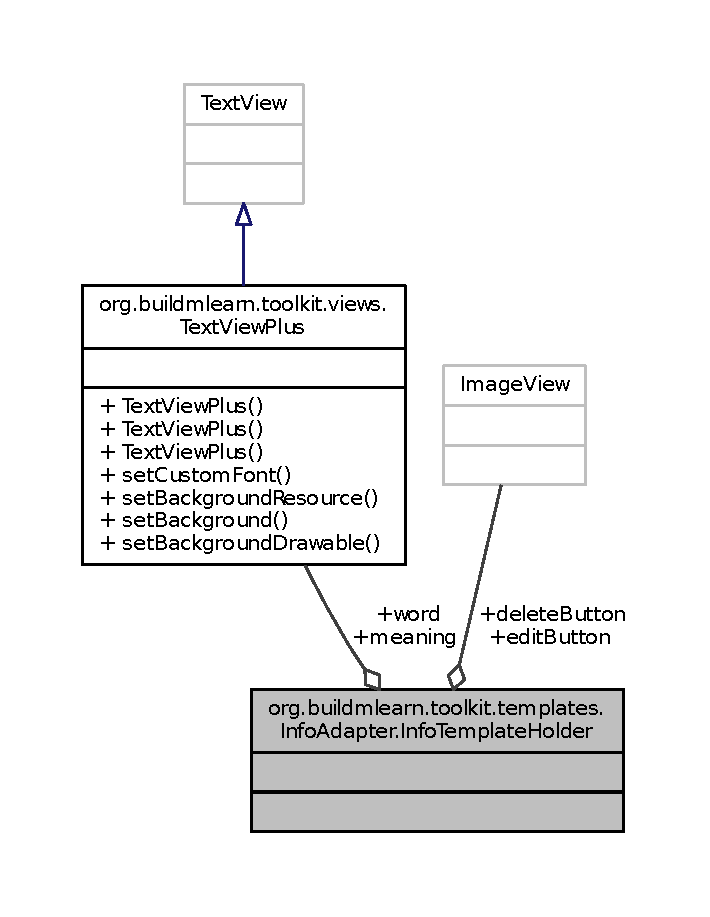
\includegraphics[width=341pt]{df/d15/classorg_1_1buildmlearn_1_1toolkit_1_1templates_1_1InfoAdapter_1_1InfoTemplateHolder__coll__graph}
\end{center}
\end{figure}
\subsection*{Public Attributes}
\begin{DoxyCompactItemize}
\item 
\hyperlink{classorg_1_1buildmlearn_1_1toolkit_1_1views_1_1TextViewPlus}{Text\-View\-Plus} \hyperlink{classorg_1_1buildmlearn_1_1toolkit_1_1templates_1_1InfoAdapter_1_1InfoTemplateHolder_a0391d141913c5ab231c1b22cc0c32a55}{word}
\item 
\hyperlink{classorg_1_1buildmlearn_1_1toolkit_1_1views_1_1TextViewPlus}{Text\-View\-Plus} \hyperlink{classorg_1_1buildmlearn_1_1toolkit_1_1templates_1_1InfoAdapter_1_1InfoTemplateHolder_a50883106775afa0b300bfad56a609dc0}{meaning}
\item 
Image\-View \hyperlink{classorg_1_1buildmlearn_1_1toolkit_1_1templates_1_1InfoAdapter_1_1InfoTemplateHolder_acdfcdf656cddda764d19e3c813b40553}{edit\-Button}
\item 
Image\-View \hyperlink{classorg_1_1buildmlearn_1_1toolkit_1_1templates_1_1InfoAdapter_1_1InfoTemplateHolder_a89300faff2511b44e9667d3e84ae371b}{delete\-Button}
\end{DoxyCompactItemize}


\subsection{Member Data Documentation}
\hypertarget{classorg_1_1buildmlearn_1_1toolkit_1_1templates_1_1InfoAdapter_1_1InfoTemplateHolder_a89300faff2511b44e9667d3e84ae371b}{\index{org\-::buildmlearn\-::toolkit\-::templates\-::\-Info\-Adapter\-::\-Info\-Template\-Holder@{org\-::buildmlearn\-::toolkit\-::templates\-::\-Info\-Adapter\-::\-Info\-Template\-Holder}!delete\-Button@{delete\-Button}}
\index{delete\-Button@{delete\-Button}!org::buildmlearn::toolkit::templates::InfoAdapter::InfoTemplateHolder@{org\-::buildmlearn\-::toolkit\-::templates\-::\-Info\-Adapter\-::\-Info\-Template\-Holder}}
\subsubsection[{delete\-Button}]{\setlength{\rightskip}{0pt plus 5cm}Image\-View org.\-buildmlearn.\-toolkit.\-templates.\-Info\-Adapter.\-Info\-Template\-Holder.\-delete\-Button}}\label{classorg_1_1buildmlearn_1_1toolkit_1_1templates_1_1InfoAdapter_1_1InfoTemplateHolder_a89300faff2511b44e9667d3e84ae371b}
\hypertarget{classorg_1_1buildmlearn_1_1toolkit_1_1templates_1_1InfoAdapter_1_1InfoTemplateHolder_acdfcdf656cddda764d19e3c813b40553}{\index{org\-::buildmlearn\-::toolkit\-::templates\-::\-Info\-Adapter\-::\-Info\-Template\-Holder@{org\-::buildmlearn\-::toolkit\-::templates\-::\-Info\-Adapter\-::\-Info\-Template\-Holder}!edit\-Button@{edit\-Button}}
\index{edit\-Button@{edit\-Button}!org::buildmlearn::toolkit::templates::InfoAdapter::InfoTemplateHolder@{org\-::buildmlearn\-::toolkit\-::templates\-::\-Info\-Adapter\-::\-Info\-Template\-Holder}}
\subsubsection[{edit\-Button}]{\setlength{\rightskip}{0pt plus 5cm}Image\-View org.\-buildmlearn.\-toolkit.\-templates.\-Info\-Adapter.\-Info\-Template\-Holder.\-edit\-Button}}\label{classorg_1_1buildmlearn_1_1toolkit_1_1templates_1_1InfoAdapter_1_1InfoTemplateHolder_acdfcdf656cddda764d19e3c813b40553}
\hypertarget{classorg_1_1buildmlearn_1_1toolkit_1_1templates_1_1InfoAdapter_1_1InfoTemplateHolder_a50883106775afa0b300bfad56a609dc0}{\index{org\-::buildmlearn\-::toolkit\-::templates\-::\-Info\-Adapter\-::\-Info\-Template\-Holder@{org\-::buildmlearn\-::toolkit\-::templates\-::\-Info\-Adapter\-::\-Info\-Template\-Holder}!meaning@{meaning}}
\index{meaning@{meaning}!org::buildmlearn::toolkit::templates::InfoAdapter::InfoTemplateHolder@{org\-::buildmlearn\-::toolkit\-::templates\-::\-Info\-Adapter\-::\-Info\-Template\-Holder}}
\subsubsection[{meaning}]{\setlength{\rightskip}{0pt plus 5cm}{\bf Text\-View\-Plus} org.\-buildmlearn.\-toolkit.\-templates.\-Info\-Adapter.\-Info\-Template\-Holder.\-meaning}}\label{classorg_1_1buildmlearn_1_1toolkit_1_1templates_1_1InfoAdapter_1_1InfoTemplateHolder_a50883106775afa0b300bfad56a609dc0}
\hypertarget{classorg_1_1buildmlearn_1_1toolkit_1_1templates_1_1InfoAdapter_1_1InfoTemplateHolder_a0391d141913c5ab231c1b22cc0c32a55}{\index{org\-::buildmlearn\-::toolkit\-::templates\-::\-Info\-Adapter\-::\-Info\-Template\-Holder@{org\-::buildmlearn\-::toolkit\-::templates\-::\-Info\-Adapter\-::\-Info\-Template\-Holder}!word@{word}}
\index{word@{word}!org::buildmlearn::toolkit::templates::InfoAdapter::InfoTemplateHolder@{org\-::buildmlearn\-::toolkit\-::templates\-::\-Info\-Adapter\-::\-Info\-Template\-Holder}}
\subsubsection[{word}]{\setlength{\rightskip}{0pt plus 5cm}{\bf Text\-View\-Plus} org.\-buildmlearn.\-toolkit.\-templates.\-Info\-Adapter.\-Info\-Template\-Holder.\-word}}\label{classorg_1_1buildmlearn_1_1toolkit_1_1templates_1_1InfoAdapter_1_1InfoTemplateHolder_a0391d141913c5ab231c1b22cc0c32a55}


The documentation for this class was generated from the following file\-:\begin{DoxyCompactItemize}
\item 
/\-Buildm\-Learn-\/\-Toolkit-\/\-Android/source-\/code/app/src/main/java/org/buildmlearn/toolkit/templates/\hyperlink{InfoAdapter_8java}{Info\-Adapter.\-java}\end{DoxyCompactItemize}

\hypertarget{classorg_1_1buildmlearn_1_1toolkit_1_1utilities_1_1Keystore}{\section{org.\-buildmlearn.\-toolkit.\-utilities.\-Keystore Class Reference}
\label{classorg_1_1buildmlearn_1_1toolkit_1_1utilities_1_1Keystore}\index{org.\-buildmlearn.\-toolkit.\-utilities.\-Keystore@{org.\-buildmlearn.\-toolkit.\-utilities.\-Keystore}}
}


Model class for storing \hyperlink{classorg_1_1buildmlearn_1_1toolkit_1_1utilities_1_1Keystore}{Keystore} details.  




Collaboration diagram for org.\-buildmlearn.\-toolkit.\-utilities.\-Keystore\-:
\nopagebreak
\begin{figure}[H]
\begin{center}
\leavevmode
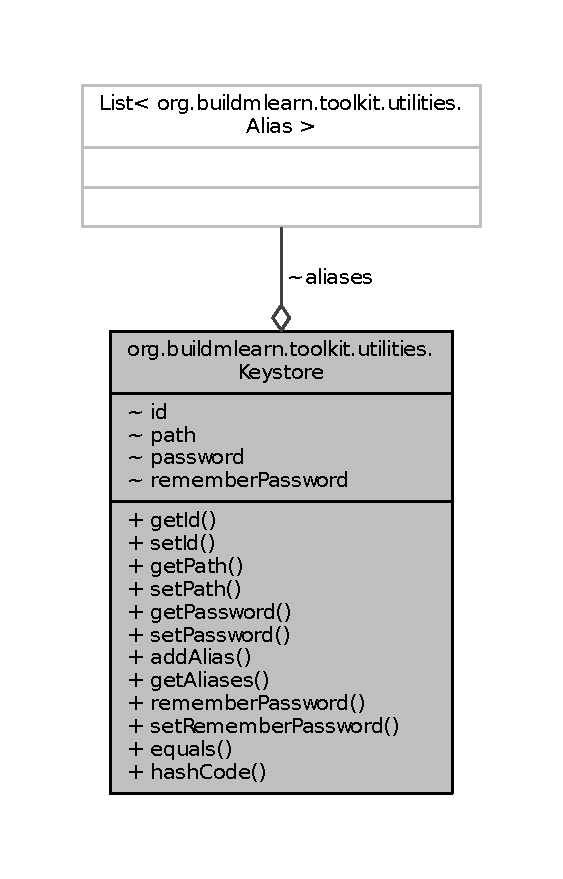
\includegraphics[width=270pt]{d5/d16/classorg_1_1buildmlearn_1_1toolkit_1_1utilities_1_1Keystore__coll__graph}
\end{center}
\end{figure}
\subsection*{Public Member Functions}
\begin{DoxyCompactItemize}
\item 
long \hyperlink{classorg_1_1buildmlearn_1_1toolkit_1_1utilities_1_1Keystore_a048b20c740a55d66b6cb4fdca4ce95fb}{get\-Id} ()
\item 
void \hyperlink{classorg_1_1buildmlearn_1_1toolkit_1_1utilities_1_1Keystore_adec03f329a7c3b142bf46f70db1efa53}{set\-Id} (long id)
\item 
String \hyperlink{classorg_1_1buildmlearn_1_1toolkit_1_1utilities_1_1Keystore_a25ab70c2cf244222465fb5636862309a}{get\-Path} ()
\item 
void \hyperlink{classorg_1_1buildmlearn_1_1toolkit_1_1utilities_1_1Keystore_a3af36a851875e2c8044573b25a26ed77}{set\-Path} (String path)
\item 
String \hyperlink{classorg_1_1buildmlearn_1_1toolkit_1_1utilities_1_1Keystore_ad8582bdf60e41657863fbb0a94a5fcc0}{get\-Password} ()
\item 
void \hyperlink{classorg_1_1buildmlearn_1_1toolkit_1_1utilities_1_1Keystore_a621acd77ce8b88953239d96c4195e02e}{set\-Password} (String password)
\item 
void \hyperlink{classorg_1_1buildmlearn_1_1toolkit_1_1utilities_1_1Keystore_aea74578df4fce4ebefdfd58d81c5563b}{add\-Alias} (\hyperlink{classorg_1_1buildmlearn_1_1toolkit_1_1utilities_1_1Alias}{Alias} alias)
\item 
List$<$ \hyperlink{classorg_1_1buildmlearn_1_1toolkit_1_1utilities_1_1Alias}{Alias} $>$ \hyperlink{classorg_1_1buildmlearn_1_1toolkit_1_1utilities_1_1Keystore_a62162a7ce16401766620c0c9a2f7af66}{get\-Aliases} ()
\item 
boolean \hyperlink{classorg_1_1buildmlearn_1_1toolkit_1_1utilities_1_1Keystore_a2e2935672133a9b9f532199eb68f23bc}{remember\-Password} ()
\item 
void \hyperlink{classorg_1_1buildmlearn_1_1toolkit_1_1utilities_1_1Keystore_a1a367d77982e10aaffb6c59e91487592}{set\-Remember\-Password} (boolean remember\-Password)
\item 
boolean \hyperlink{classorg_1_1buildmlearn_1_1toolkit_1_1utilities_1_1Keystore_a5e6bcbcdcad101723cc8f22a09996490}{equals} (Object o)
\item 
int \hyperlink{classorg_1_1buildmlearn_1_1toolkit_1_1utilities_1_1Keystore_acb6c19ecbe0d7c98e0c8f3f4092e6ab8}{hash\-Code} ()
\end{DoxyCompactItemize}


\subsection{Detailed Description}
Model class for storing \hyperlink{classorg_1_1buildmlearn_1_1toolkit_1_1utilities_1_1Keystore}{Keystore} details. 

\subsection{Member Function Documentation}
\hypertarget{classorg_1_1buildmlearn_1_1toolkit_1_1utilities_1_1Keystore_aea74578df4fce4ebefdfd58d81c5563b}{\index{org\-::buildmlearn\-::toolkit\-::utilities\-::\-Keystore@{org\-::buildmlearn\-::toolkit\-::utilities\-::\-Keystore}!add\-Alias@{add\-Alias}}
\index{add\-Alias@{add\-Alias}!org::buildmlearn::toolkit::utilities::Keystore@{org\-::buildmlearn\-::toolkit\-::utilities\-::\-Keystore}}
\subsubsection[{add\-Alias}]{\setlength{\rightskip}{0pt plus 5cm}void org.\-buildmlearn.\-toolkit.\-utilities.\-Keystore.\-add\-Alias (
\begin{DoxyParamCaption}
\item[{{\bf Alias}}]{alias}
\end{DoxyParamCaption}
)}}\label{classorg_1_1buildmlearn_1_1toolkit_1_1utilities_1_1Keystore_aea74578df4fce4ebefdfd58d81c5563b}

\begin{DoxyCode}
43                                       \{
44         aliases.add(alias);
45     \}
\end{DoxyCode}
\hypertarget{classorg_1_1buildmlearn_1_1toolkit_1_1utilities_1_1Keystore_a5e6bcbcdcad101723cc8f22a09996490}{\index{org\-::buildmlearn\-::toolkit\-::utilities\-::\-Keystore@{org\-::buildmlearn\-::toolkit\-::utilities\-::\-Keystore}!equals@{equals}}
\index{equals@{equals}!org::buildmlearn::toolkit::utilities::Keystore@{org\-::buildmlearn\-::toolkit\-::utilities\-::\-Keystore}}
\subsubsection[{equals}]{\setlength{\rightskip}{0pt plus 5cm}boolean org.\-buildmlearn.\-toolkit.\-utilities.\-Keystore.\-equals (
\begin{DoxyParamCaption}
\item[{Object}]{o}
\end{DoxyParamCaption}
)}}\label{classorg_1_1buildmlearn_1_1toolkit_1_1utilities_1_1Keystore_a5e6bcbcdcad101723cc8f22a09996490}

\begin{DoxyCode}
60                                     \{
61         \textcolor{keywordflow}{if} (\textcolor{keyword}{this} == o) \textcolor{keywordflow}{return} \textcolor{keyword}{true};
62         \textcolor{keywordflow}{if} (o == null || getClass() != o.getClass()) \textcolor{keywordflow}{return} \textcolor{keyword}{false};
63 
64         Keystore keystore = (Keystore) o;
65 
66         \textcolor{keywordflow}{if} (\textcolor{keywordtype}{id} != keystore.id) \textcolor{keywordflow}{return} \textcolor{keyword}{false};
67 
68         \textcolor{keywordflow}{return} \textcolor{keyword}{true};
69     \}
\end{DoxyCode}
\hypertarget{classorg_1_1buildmlearn_1_1toolkit_1_1utilities_1_1Keystore_a62162a7ce16401766620c0c9a2f7af66}{\index{org\-::buildmlearn\-::toolkit\-::utilities\-::\-Keystore@{org\-::buildmlearn\-::toolkit\-::utilities\-::\-Keystore}!get\-Aliases@{get\-Aliases}}
\index{get\-Aliases@{get\-Aliases}!org::buildmlearn::toolkit::utilities::Keystore@{org\-::buildmlearn\-::toolkit\-::utilities\-::\-Keystore}}
\subsubsection[{get\-Aliases}]{\setlength{\rightskip}{0pt plus 5cm}List$<${\bf Alias}$>$ org.\-buildmlearn.\-toolkit.\-utilities.\-Keystore.\-get\-Aliases (
\begin{DoxyParamCaption}
{}
\end{DoxyParamCaption}
)}}\label{classorg_1_1buildmlearn_1_1toolkit_1_1utilities_1_1Keystore_a62162a7ce16401766620c0c9a2f7af66}

\begin{DoxyCode}
47                                     \{
48         \textcolor{keywordflow}{return} aliases;
49     \}
\end{DoxyCode}
\hypertarget{classorg_1_1buildmlearn_1_1toolkit_1_1utilities_1_1Keystore_a048b20c740a55d66b6cb4fdca4ce95fb}{\index{org\-::buildmlearn\-::toolkit\-::utilities\-::\-Keystore@{org\-::buildmlearn\-::toolkit\-::utilities\-::\-Keystore}!get\-Id@{get\-Id}}
\index{get\-Id@{get\-Id}!org::buildmlearn::toolkit::utilities::Keystore@{org\-::buildmlearn\-::toolkit\-::utilities\-::\-Keystore}}
\subsubsection[{get\-Id}]{\setlength{\rightskip}{0pt plus 5cm}long org.\-buildmlearn.\-toolkit.\-utilities.\-Keystore.\-get\-Id (
\begin{DoxyParamCaption}
{}
\end{DoxyParamCaption}
)}}\label{classorg_1_1buildmlearn_1_1toolkit_1_1utilities_1_1Keystore_a048b20c740a55d66b6cb4fdca4ce95fb}

\begin{DoxyCode}
19                         \{
20         \textcolor{keywordflow}{return} id;
21     \}
\end{DoxyCode}
\hypertarget{classorg_1_1buildmlearn_1_1toolkit_1_1utilities_1_1Keystore_ad8582bdf60e41657863fbb0a94a5fcc0}{\index{org\-::buildmlearn\-::toolkit\-::utilities\-::\-Keystore@{org\-::buildmlearn\-::toolkit\-::utilities\-::\-Keystore}!get\-Password@{get\-Password}}
\index{get\-Password@{get\-Password}!org::buildmlearn::toolkit::utilities::Keystore@{org\-::buildmlearn\-::toolkit\-::utilities\-::\-Keystore}}
\subsubsection[{get\-Password}]{\setlength{\rightskip}{0pt plus 5cm}String org.\-buildmlearn.\-toolkit.\-utilities.\-Keystore.\-get\-Password (
\begin{DoxyParamCaption}
{}
\end{DoxyParamCaption}
)}}\label{classorg_1_1buildmlearn_1_1toolkit_1_1utilities_1_1Keystore_ad8582bdf60e41657863fbb0a94a5fcc0}

\begin{DoxyCode}
35                                 \{
36         \textcolor{keywordflow}{return} password;
37     \}
\end{DoxyCode}
\hypertarget{classorg_1_1buildmlearn_1_1toolkit_1_1utilities_1_1Keystore_a25ab70c2cf244222465fb5636862309a}{\index{org\-::buildmlearn\-::toolkit\-::utilities\-::\-Keystore@{org\-::buildmlearn\-::toolkit\-::utilities\-::\-Keystore}!get\-Path@{get\-Path}}
\index{get\-Path@{get\-Path}!org::buildmlearn::toolkit::utilities::Keystore@{org\-::buildmlearn\-::toolkit\-::utilities\-::\-Keystore}}
\subsubsection[{get\-Path}]{\setlength{\rightskip}{0pt plus 5cm}String org.\-buildmlearn.\-toolkit.\-utilities.\-Keystore.\-get\-Path (
\begin{DoxyParamCaption}
{}
\end{DoxyParamCaption}
)}}\label{classorg_1_1buildmlearn_1_1toolkit_1_1utilities_1_1Keystore_a25ab70c2cf244222465fb5636862309a}

\begin{DoxyCode}
27                             \{
28         \textcolor{keywordflow}{return} path;
29     \}
\end{DoxyCode}
\hypertarget{classorg_1_1buildmlearn_1_1toolkit_1_1utilities_1_1Keystore_acb6c19ecbe0d7c98e0c8f3f4092e6ab8}{\index{org\-::buildmlearn\-::toolkit\-::utilities\-::\-Keystore@{org\-::buildmlearn\-::toolkit\-::utilities\-::\-Keystore}!hash\-Code@{hash\-Code}}
\index{hash\-Code@{hash\-Code}!org::buildmlearn::toolkit::utilities::Keystore@{org\-::buildmlearn\-::toolkit\-::utilities\-::\-Keystore}}
\subsubsection[{hash\-Code}]{\setlength{\rightskip}{0pt plus 5cm}int org.\-buildmlearn.\-toolkit.\-utilities.\-Keystore.\-hash\-Code (
\begin{DoxyParamCaption}
{}
\end{DoxyParamCaption}
)}}\label{classorg_1_1buildmlearn_1_1toolkit_1_1utilities_1_1Keystore_acb6c19ecbe0d7c98e0c8f3f4092e6ab8}

\begin{DoxyCode}
72                           \{
73         \textcolor{keywordflow}{return} (\textcolor{keywordtype}{int}) (\textcolor{keywordtype}{id} ^ (\textcolor{keywordtype}{id} >>> 32));
74     \}
\end{DoxyCode}
\hypertarget{classorg_1_1buildmlearn_1_1toolkit_1_1utilities_1_1Keystore_a2e2935672133a9b9f532199eb68f23bc}{\index{org\-::buildmlearn\-::toolkit\-::utilities\-::\-Keystore@{org\-::buildmlearn\-::toolkit\-::utilities\-::\-Keystore}!remember\-Password@{remember\-Password}}
\index{remember\-Password@{remember\-Password}!org::buildmlearn::toolkit::utilities::Keystore@{org\-::buildmlearn\-::toolkit\-::utilities\-::\-Keystore}}
\subsubsection[{remember\-Password}]{\setlength{\rightskip}{0pt plus 5cm}boolean org.\-buildmlearn.\-toolkit.\-utilities.\-Keystore.\-remember\-Password (
\begin{DoxyParamCaption}
{}
\end{DoxyParamCaption}
)}}\label{classorg_1_1buildmlearn_1_1toolkit_1_1utilities_1_1Keystore_a2e2935672133a9b9f532199eb68f23bc}

\begin{DoxyCode}
51                                       \{
52         \textcolor{keywordflow}{return} \hyperlink{classorg_1_1buildmlearn_1_1toolkit_1_1utilities_1_1Keystore_a2e2935672133a9b9f532199eb68f23bc}{rememberPassword};
53     \}
\end{DoxyCode}
\hypertarget{classorg_1_1buildmlearn_1_1toolkit_1_1utilities_1_1Keystore_adec03f329a7c3b142bf46f70db1efa53}{\index{org\-::buildmlearn\-::toolkit\-::utilities\-::\-Keystore@{org\-::buildmlearn\-::toolkit\-::utilities\-::\-Keystore}!set\-Id@{set\-Id}}
\index{set\-Id@{set\-Id}!org::buildmlearn::toolkit::utilities::Keystore@{org\-::buildmlearn\-::toolkit\-::utilities\-::\-Keystore}}
\subsubsection[{set\-Id}]{\setlength{\rightskip}{0pt plus 5cm}void org.\-buildmlearn.\-toolkit.\-utilities.\-Keystore.\-set\-Id (
\begin{DoxyParamCaption}
\item[{long}]{id}
\end{DoxyParamCaption}
)}}\label{classorg_1_1buildmlearn_1_1toolkit_1_1utilities_1_1Keystore_adec03f329a7c3b142bf46f70db1efa53}

\begin{DoxyCode}
23                                \{
24         this.id = id;
25     \}
\end{DoxyCode}
\hypertarget{classorg_1_1buildmlearn_1_1toolkit_1_1utilities_1_1Keystore_a621acd77ce8b88953239d96c4195e02e}{\index{org\-::buildmlearn\-::toolkit\-::utilities\-::\-Keystore@{org\-::buildmlearn\-::toolkit\-::utilities\-::\-Keystore}!set\-Password@{set\-Password}}
\index{set\-Password@{set\-Password}!org::buildmlearn::toolkit::utilities::Keystore@{org\-::buildmlearn\-::toolkit\-::utilities\-::\-Keystore}}
\subsubsection[{set\-Password}]{\setlength{\rightskip}{0pt plus 5cm}void org.\-buildmlearn.\-toolkit.\-utilities.\-Keystore.\-set\-Password (
\begin{DoxyParamCaption}
\item[{String}]{password}
\end{DoxyParamCaption}
)}}\label{classorg_1_1buildmlearn_1_1toolkit_1_1utilities_1_1Keystore_a621acd77ce8b88953239d96c4195e02e}

\begin{DoxyCode}
39                                              \{
40         this.password = password;
41     \}
\end{DoxyCode}
\hypertarget{classorg_1_1buildmlearn_1_1toolkit_1_1utilities_1_1Keystore_a3af36a851875e2c8044573b25a26ed77}{\index{org\-::buildmlearn\-::toolkit\-::utilities\-::\-Keystore@{org\-::buildmlearn\-::toolkit\-::utilities\-::\-Keystore}!set\-Path@{set\-Path}}
\index{set\-Path@{set\-Path}!org::buildmlearn::toolkit::utilities::Keystore@{org\-::buildmlearn\-::toolkit\-::utilities\-::\-Keystore}}
\subsubsection[{set\-Path}]{\setlength{\rightskip}{0pt plus 5cm}void org.\-buildmlearn.\-toolkit.\-utilities.\-Keystore.\-set\-Path (
\begin{DoxyParamCaption}
\item[{String}]{path}
\end{DoxyParamCaption}
)}}\label{classorg_1_1buildmlearn_1_1toolkit_1_1utilities_1_1Keystore_a3af36a851875e2c8044573b25a26ed77}

\begin{DoxyCode}
31                                      \{
32         this.path = path;
33     \}
\end{DoxyCode}
\hypertarget{classorg_1_1buildmlearn_1_1toolkit_1_1utilities_1_1Keystore_a1a367d77982e10aaffb6c59e91487592}{\index{org\-::buildmlearn\-::toolkit\-::utilities\-::\-Keystore@{org\-::buildmlearn\-::toolkit\-::utilities\-::\-Keystore}!set\-Remember\-Password@{set\-Remember\-Password}}
\index{set\-Remember\-Password@{set\-Remember\-Password}!org::buildmlearn::toolkit::utilities::Keystore@{org\-::buildmlearn\-::toolkit\-::utilities\-::\-Keystore}}
\subsubsection[{set\-Remember\-Password}]{\setlength{\rightskip}{0pt plus 5cm}void org.\-buildmlearn.\-toolkit.\-utilities.\-Keystore.\-set\-Remember\-Password (
\begin{DoxyParamCaption}
\item[{boolean}]{remember\-Password}
\end{DoxyParamCaption}
)}}\label{classorg_1_1buildmlearn_1_1toolkit_1_1utilities_1_1Keystore_a1a367d77982e10aaffb6c59e91487592}

\begin{DoxyCode}
55                                                               \{
56         this.rememberPassword = \hyperlink{classorg_1_1buildmlearn_1_1toolkit_1_1utilities_1_1Keystore_a2e2935672133a9b9f532199eb68f23bc}{rememberPassword};
57     \}
\end{DoxyCode}


The documentation for this class was generated from the following file\-:\begin{DoxyCompactItemize}
\item 
/\-Buildm\-Learn-\/\-Toolkit-\/\-Android/source-\/code/app/src/main/java/org/buildmlearn/toolkit/utilities/\hyperlink{Keystore_8java}{Keystore.\-java}\end{DoxyCompactItemize}

\hypertarget{classorg_1_1buildmlearn_1_1toolkit_1_1model_1_1KeyStoreDetails}{\section{org.\-buildmlearn.\-toolkit.\-model.\-Key\-Store\-Details Class Reference}
\label{classorg_1_1buildmlearn_1_1toolkit_1_1model_1_1KeyStoreDetails}\index{org.\-buildmlearn.\-toolkit.\-model.\-Key\-Store\-Details@{org.\-buildmlearn.\-toolkit.\-model.\-Key\-Store\-Details}}
}


Model class for holding the details of keystore file.  




Collaboration diagram for org.\-buildmlearn.\-toolkit.\-model.\-Key\-Store\-Details\-:
\nopagebreak
\begin{figure}[H]
\begin{center}
\leavevmode
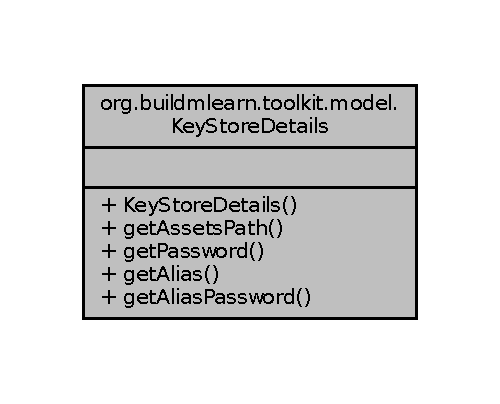
\includegraphics[width=240pt]{da/dad/classorg_1_1buildmlearn_1_1toolkit_1_1model_1_1KeyStoreDetails__coll__graph}
\end{center}
\end{figure}
\subsection*{Public Member Functions}
\begin{DoxyCompactItemize}
\item 
\hyperlink{classorg_1_1buildmlearn_1_1toolkit_1_1model_1_1KeyStoreDetails_a8928a74a82e98926ce0090ceb85a7d3f}{Key\-Store\-Details} (String assets\-Path, String password, String alias, String alias\-Password)
\item 
String \hyperlink{classorg_1_1buildmlearn_1_1toolkit_1_1model_1_1KeyStoreDetails_ab3f06172d5a670983b711d3b32c6b742}{get\-Assets\-Path} ()
\item 
String \hyperlink{classorg_1_1buildmlearn_1_1toolkit_1_1model_1_1KeyStoreDetails_afab09fb7d5ad40c70ce0e1c7df720eb5}{get\-Password} ()
\item 
String \hyperlink{classorg_1_1buildmlearn_1_1toolkit_1_1model_1_1KeyStoreDetails_a27f0dbd2433e3b1044b8fceda27ab4ac}{get\-Alias} ()
\item 
String \hyperlink{classorg_1_1buildmlearn_1_1toolkit_1_1model_1_1KeyStoreDetails_ac9f20a209c0509b7d19d9949a5ba7831}{get\-Alias\-Password} ()
\end{DoxyCompactItemize}


\subsection{Detailed Description}
Model class for holding the details of keystore file. 

Created by abhishek on 11/06/15 at 2\-:19 P\-M. 

\subsection{Constructor \& Destructor Documentation}
\hypertarget{classorg_1_1buildmlearn_1_1toolkit_1_1model_1_1KeyStoreDetails_a8928a74a82e98926ce0090ceb85a7d3f}{\index{org\-::buildmlearn\-::toolkit\-::model\-::\-Key\-Store\-Details@{org\-::buildmlearn\-::toolkit\-::model\-::\-Key\-Store\-Details}!Key\-Store\-Details@{Key\-Store\-Details}}
\index{Key\-Store\-Details@{Key\-Store\-Details}!org::buildmlearn::toolkit::model::KeyStoreDetails@{org\-::buildmlearn\-::toolkit\-::model\-::\-Key\-Store\-Details}}
\subsubsection[{Key\-Store\-Details}]{\setlength{\rightskip}{0pt plus 5cm}org.\-buildmlearn.\-toolkit.\-model.\-Key\-Store\-Details.\-Key\-Store\-Details (
\begin{DoxyParamCaption}
\item[{String}]{assets\-Path, }
\item[{String}]{password, }
\item[{String}]{alias, }
\item[{String}]{alias\-Password}
\end{DoxyParamCaption}
)}}\label{classorg_1_1buildmlearn_1_1toolkit_1_1model_1_1KeyStoreDetails_a8928a74a82e98926ce0090ceb85a7d3f}

\begin{DoxyCode}
15                                                                                                    \{
16         this.assetsPath = assetsPath;
17         this.password = password;
18         this.alias = alias;
19         this.aliasPassword = aliasPassword;
20     \}
\end{DoxyCode}


\subsection{Member Function Documentation}
\hypertarget{classorg_1_1buildmlearn_1_1toolkit_1_1model_1_1KeyStoreDetails_a27f0dbd2433e3b1044b8fceda27ab4ac}{\index{org\-::buildmlearn\-::toolkit\-::model\-::\-Key\-Store\-Details@{org\-::buildmlearn\-::toolkit\-::model\-::\-Key\-Store\-Details}!get\-Alias@{get\-Alias}}
\index{get\-Alias@{get\-Alias}!org::buildmlearn::toolkit::model::KeyStoreDetails@{org\-::buildmlearn\-::toolkit\-::model\-::\-Key\-Store\-Details}}
\subsubsection[{get\-Alias}]{\setlength{\rightskip}{0pt plus 5cm}String org.\-buildmlearn.\-toolkit.\-model.\-Key\-Store\-Details.\-get\-Alias (
\begin{DoxyParamCaption}
{}
\end{DoxyParamCaption}
)}}\label{classorg_1_1buildmlearn_1_1toolkit_1_1model_1_1KeyStoreDetails_a27f0dbd2433e3b1044b8fceda27ab4ac}

\begin{DoxyCode}
30                              \{
31         \textcolor{keywordflow}{return} alias;
32     \}
\end{DoxyCode}
\hypertarget{classorg_1_1buildmlearn_1_1toolkit_1_1model_1_1KeyStoreDetails_ac9f20a209c0509b7d19d9949a5ba7831}{\index{org\-::buildmlearn\-::toolkit\-::model\-::\-Key\-Store\-Details@{org\-::buildmlearn\-::toolkit\-::model\-::\-Key\-Store\-Details}!get\-Alias\-Password@{get\-Alias\-Password}}
\index{get\-Alias\-Password@{get\-Alias\-Password}!org::buildmlearn::toolkit::model::KeyStoreDetails@{org\-::buildmlearn\-::toolkit\-::model\-::\-Key\-Store\-Details}}
\subsubsection[{get\-Alias\-Password}]{\setlength{\rightskip}{0pt plus 5cm}String org.\-buildmlearn.\-toolkit.\-model.\-Key\-Store\-Details.\-get\-Alias\-Password (
\begin{DoxyParamCaption}
{}
\end{DoxyParamCaption}
)}}\label{classorg_1_1buildmlearn_1_1toolkit_1_1model_1_1KeyStoreDetails_ac9f20a209c0509b7d19d9949a5ba7831}

\begin{DoxyCode}
34                                      \{
35         \textcolor{keywordflow}{return} aliasPassword;
36     \}
\end{DoxyCode}
\hypertarget{classorg_1_1buildmlearn_1_1toolkit_1_1model_1_1KeyStoreDetails_ab3f06172d5a670983b711d3b32c6b742}{\index{org\-::buildmlearn\-::toolkit\-::model\-::\-Key\-Store\-Details@{org\-::buildmlearn\-::toolkit\-::model\-::\-Key\-Store\-Details}!get\-Assets\-Path@{get\-Assets\-Path}}
\index{get\-Assets\-Path@{get\-Assets\-Path}!org::buildmlearn::toolkit::model::KeyStoreDetails@{org\-::buildmlearn\-::toolkit\-::model\-::\-Key\-Store\-Details}}
\subsubsection[{get\-Assets\-Path}]{\setlength{\rightskip}{0pt plus 5cm}String org.\-buildmlearn.\-toolkit.\-model.\-Key\-Store\-Details.\-get\-Assets\-Path (
\begin{DoxyParamCaption}
{}
\end{DoxyParamCaption}
)}}\label{classorg_1_1buildmlearn_1_1toolkit_1_1model_1_1KeyStoreDetails_ab3f06172d5a670983b711d3b32c6b742}

\begin{DoxyCode}
22                                   \{
23         \textcolor{keywordflow}{return} assetsPath;
24     \}
\end{DoxyCode}
\hypertarget{classorg_1_1buildmlearn_1_1toolkit_1_1model_1_1KeyStoreDetails_afab09fb7d5ad40c70ce0e1c7df720eb5}{\index{org\-::buildmlearn\-::toolkit\-::model\-::\-Key\-Store\-Details@{org\-::buildmlearn\-::toolkit\-::model\-::\-Key\-Store\-Details}!get\-Password@{get\-Password}}
\index{get\-Password@{get\-Password}!org::buildmlearn::toolkit::model::KeyStoreDetails@{org\-::buildmlearn\-::toolkit\-::model\-::\-Key\-Store\-Details}}
\subsubsection[{get\-Password}]{\setlength{\rightskip}{0pt plus 5cm}String org.\-buildmlearn.\-toolkit.\-model.\-Key\-Store\-Details.\-get\-Password (
\begin{DoxyParamCaption}
{}
\end{DoxyParamCaption}
)}}\label{classorg_1_1buildmlearn_1_1toolkit_1_1model_1_1KeyStoreDetails_afab09fb7d5ad40c70ce0e1c7df720eb5}

\begin{DoxyCode}
26                                 \{
27         \textcolor{keywordflow}{return} password;
28     \}
\end{DoxyCode}


The documentation for this class was generated from the following file\-:\begin{DoxyCompactItemize}
\item 
/\-Buildm\-Learn-\/\-Toolkit-\/\-Android/source-\/code/app/src/main/java/org/buildmlearn/toolkit/model/\hyperlink{KeyStoreDetails_8java}{Key\-Store\-Details.\-java}\end{DoxyCompactItemize}

\hypertarget{classorg_1_1buildmlearn_1_1toolkit_1_1templates_1_1LearnSpellingAdapter}{\section{org.\-buildmlearn.\-toolkit.\-templates.\-Learn\-Spelling\-Adapter Class Reference}
\label{classorg_1_1buildmlearn_1_1toolkit_1_1templates_1_1LearnSpellingAdapter}\index{org.\-buildmlearn.\-toolkit.\-templates.\-Learn\-Spelling\-Adapter@{org.\-buildmlearn.\-toolkit.\-templates.\-Learn\-Spelling\-Adapter}}
}


Adapter for displaying Learn Spelling Template Editor data.  




Inheritance diagram for org.\-buildmlearn.\-toolkit.\-templates.\-Learn\-Spelling\-Adapter\-:
\nopagebreak
\begin{figure}[H]
\begin{center}
\leavevmode
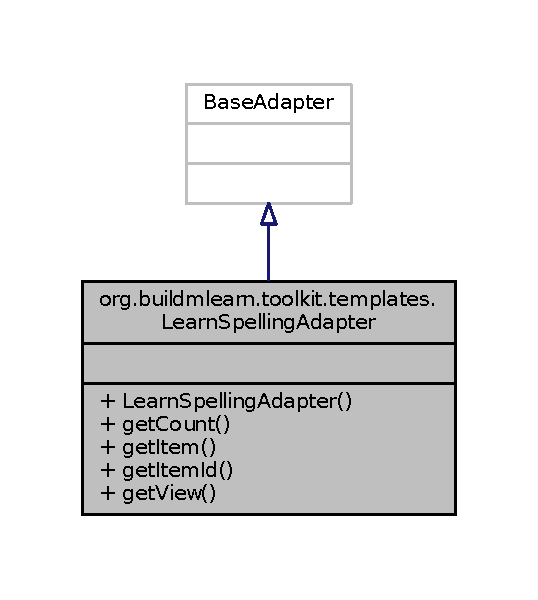
\includegraphics[width=258pt]{d7/ddc/classorg_1_1buildmlearn_1_1toolkit_1_1templates_1_1LearnSpellingAdapter__inherit__graph}
\end{center}
\end{figure}


Collaboration diagram for org.\-buildmlearn.\-toolkit.\-templates.\-Learn\-Spelling\-Adapter\-:
\nopagebreak
\begin{figure}[H]
\begin{center}
\leavevmode
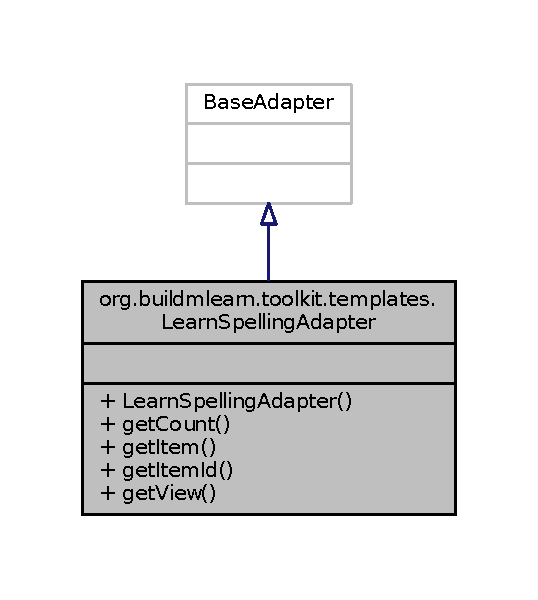
\includegraphics[width=258pt]{d9/d6e/classorg_1_1buildmlearn_1_1toolkit_1_1templates_1_1LearnSpellingAdapter__coll__graph}
\end{center}
\end{figure}
\subsection*{Classes}
\begin{DoxyCompactItemize}
\item 
class \hyperlink{classorg_1_1buildmlearn_1_1toolkit_1_1templates_1_1LearnSpellingAdapter_1_1LearnSpellingHolder}{Learn\-Spelling\-Holder}
\end{DoxyCompactItemize}
\subsection*{Public Member Functions}
\begin{DoxyCompactItemize}
\item 
\hyperlink{classorg_1_1buildmlearn_1_1toolkit_1_1templates_1_1LearnSpellingAdapter_a7d6a79b3c3da83e213a1a606fca26083}{Learn\-Spelling\-Adapter} (Context m\-Context, Array\-List$<$ \hyperlink{classorg_1_1buildmlearn_1_1toolkit_1_1templates_1_1LearnSpellingModel}{Learn\-Spelling\-Model} $>$ data)
\item 
int \hyperlink{classorg_1_1buildmlearn_1_1toolkit_1_1templates_1_1LearnSpellingAdapter_aa03e460bd84bbd1fb5d4ac881e859256}{get\-Count} ()
\item 
\hyperlink{classorg_1_1buildmlearn_1_1toolkit_1_1templates_1_1LearnSpellingModel}{Learn\-Spelling\-Model} \hyperlink{classorg_1_1buildmlearn_1_1toolkit_1_1templates_1_1LearnSpellingAdapter_af0b0934c215c709326ded3e7fc3b56aa}{get\-Item} (int position)
\item 
long \hyperlink{classorg_1_1buildmlearn_1_1toolkit_1_1templates_1_1LearnSpellingAdapter_a6fb76396d65194c3e447ec6883124564}{get\-Item\-Id} (int position)
\item 
View \hyperlink{classorg_1_1buildmlearn_1_1toolkit_1_1templates_1_1LearnSpellingAdapter_abdf6a7e409727aff2ac23c6b1993ee04}{get\-View} (final int position, View convert\-View, View\-Group parent)
\end{DoxyCompactItemize}


\subsection{Detailed Description}
Adapter for displaying Learn Spelling Template Editor data. 

Created by abhishek on 17/06/15 at 9\-:48 P\-M. 

\subsection{Constructor \& Destructor Documentation}
\hypertarget{classorg_1_1buildmlearn_1_1toolkit_1_1templates_1_1LearnSpellingAdapter_a7d6a79b3c3da83e213a1a606fca26083}{\index{org\-::buildmlearn\-::toolkit\-::templates\-::\-Learn\-Spelling\-Adapter@{org\-::buildmlearn\-::toolkit\-::templates\-::\-Learn\-Spelling\-Adapter}!Learn\-Spelling\-Adapter@{Learn\-Spelling\-Adapter}}
\index{Learn\-Spelling\-Adapter@{Learn\-Spelling\-Adapter}!org::buildmlearn::toolkit::templates::LearnSpellingAdapter@{org\-::buildmlearn\-::toolkit\-::templates\-::\-Learn\-Spelling\-Adapter}}
\subsubsection[{Learn\-Spelling\-Adapter}]{\setlength{\rightskip}{0pt plus 5cm}org.\-buildmlearn.\-toolkit.\-templates.\-Learn\-Spelling\-Adapter.\-Learn\-Spelling\-Adapter (
\begin{DoxyParamCaption}
\item[{Context}]{m\-Context, }
\item[{Array\-List$<$ {\bf Learn\-Spelling\-Model} $>$}]{data}
\end{DoxyParamCaption}
)}}\label{classorg_1_1buildmlearn_1_1toolkit_1_1templates_1_1LearnSpellingAdapter_a7d6a79b3c3da83e213a1a606fca26083}

\begin{DoxyCode}
29                                                                                       \{
30         this.mContext = mContext;
31         this.data = data;
32     \}
\end{DoxyCode}


\subsection{Member Function Documentation}
\hypertarget{classorg_1_1buildmlearn_1_1toolkit_1_1templates_1_1LearnSpellingAdapter_aa03e460bd84bbd1fb5d4ac881e859256}{\index{org\-::buildmlearn\-::toolkit\-::templates\-::\-Learn\-Spelling\-Adapter@{org\-::buildmlearn\-::toolkit\-::templates\-::\-Learn\-Spelling\-Adapter}!get\-Count@{get\-Count}}
\index{get\-Count@{get\-Count}!org::buildmlearn::toolkit::templates::LearnSpellingAdapter@{org\-::buildmlearn\-::toolkit\-::templates\-::\-Learn\-Spelling\-Adapter}}
\subsubsection[{get\-Count}]{\setlength{\rightskip}{0pt plus 5cm}int org.\-buildmlearn.\-toolkit.\-templates.\-Learn\-Spelling\-Adapter.\-get\-Count (
\begin{DoxyParamCaption}
{}
\end{DoxyParamCaption}
)}}\label{classorg_1_1buildmlearn_1_1toolkit_1_1templates_1_1LearnSpellingAdapter_aa03e460bd84bbd1fb5d4ac881e859256}

\begin{DoxyCode}
35                           \{
36         \textcolor{keywordflow}{return} data.size();
37     \}
\end{DoxyCode}
\hypertarget{classorg_1_1buildmlearn_1_1toolkit_1_1templates_1_1LearnSpellingAdapter_af0b0934c215c709326ded3e7fc3b56aa}{\index{org\-::buildmlearn\-::toolkit\-::templates\-::\-Learn\-Spelling\-Adapter@{org\-::buildmlearn\-::toolkit\-::templates\-::\-Learn\-Spelling\-Adapter}!get\-Item@{get\-Item}}
\index{get\-Item@{get\-Item}!org::buildmlearn::toolkit::templates::LearnSpellingAdapter@{org\-::buildmlearn\-::toolkit\-::templates\-::\-Learn\-Spelling\-Adapter}}
\subsubsection[{get\-Item}]{\setlength{\rightskip}{0pt plus 5cm}{\bf Learn\-Spelling\-Model} org.\-buildmlearn.\-toolkit.\-templates.\-Learn\-Spelling\-Adapter.\-get\-Item (
\begin{DoxyParamCaption}
\item[{int}]{position}
\end{DoxyParamCaption}
)}}\label{classorg_1_1buildmlearn_1_1toolkit_1_1templates_1_1LearnSpellingAdapter_af0b0934c215c709326ded3e7fc3b56aa}

\begin{DoxyCode}
40                                                     \{
41         \textcolor{keywordflow}{return} data.get(position);
42     \}
\end{DoxyCode}
\hypertarget{classorg_1_1buildmlearn_1_1toolkit_1_1templates_1_1LearnSpellingAdapter_a6fb76396d65194c3e447ec6883124564}{\index{org\-::buildmlearn\-::toolkit\-::templates\-::\-Learn\-Spelling\-Adapter@{org\-::buildmlearn\-::toolkit\-::templates\-::\-Learn\-Spelling\-Adapter}!get\-Item\-Id@{get\-Item\-Id}}
\index{get\-Item\-Id@{get\-Item\-Id}!org::buildmlearn::toolkit::templates::LearnSpellingAdapter@{org\-::buildmlearn\-::toolkit\-::templates\-::\-Learn\-Spelling\-Adapter}}
\subsubsection[{get\-Item\-Id}]{\setlength{\rightskip}{0pt plus 5cm}long org.\-buildmlearn.\-toolkit.\-templates.\-Learn\-Spelling\-Adapter.\-get\-Item\-Id (
\begin{DoxyParamCaption}
\item[{int}]{position}
\end{DoxyParamCaption}
)}}\label{classorg_1_1buildmlearn_1_1toolkit_1_1templates_1_1LearnSpellingAdapter_a6fb76396d65194c3e447ec6883124564}

\begin{DoxyCode}
45                                         \{
46         \textcolor{keywordflow}{return} position;
47     \}
\end{DoxyCode}
\hypertarget{classorg_1_1buildmlearn_1_1toolkit_1_1templates_1_1LearnSpellingAdapter_abdf6a7e409727aff2ac23c6b1993ee04}{\index{org\-::buildmlearn\-::toolkit\-::templates\-::\-Learn\-Spelling\-Adapter@{org\-::buildmlearn\-::toolkit\-::templates\-::\-Learn\-Spelling\-Adapter}!get\-View@{get\-View}}
\index{get\-View@{get\-View}!org::buildmlearn::toolkit::templates::LearnSpellingAdapter@{org\-::buildmlearn\-::toolkit\-::templates\-::\-Learn\-Spelling\-Adapter}}
\subsubsection[{get\-View}]{\setlength{\rightskip}{0pt plus 5cm}View org.\-buildmlearn.\-toolkit.\-templates.\-Learn\-Spelling\-Adapter.\-get\-View (
\begin{DoxyParamCaption}
\item[{final int}]{position, }
\item[{View}]{convert\-View, }
\item[{View\-Group}]{parent}
\end{DoxyParamCaption}
)}}\label{classorg_1_1buildmlearn_1_1toolkit_1_1templates_1_1LearnSpellingAdapter_abdf6a7e409727aff2ac23c6b1993ee04}

\begin{DoxyCode}
50                                                                                 \{
51 
52         LearnSpellingHolder holder;
53 
54         \textcolor{keywordflow}{if} (convertView == null) \{
55             LayoutInflater inflater = LayoutInflater.from(mContext);
56             convertView = inflater.inflate(R.layout.info\_template\_item, parent, \textcolor{keyword}{false});
57             holder = \textcolor{keyword}{new} LearnSpellingHolder();
58         \} \textcolor{keywordflow}{else} \{
59             holder = (LearnSpellingHolder) convertView.getTag();
60         \}
61 
62         holder.word = (TextViewPlus) convertView.findViewById(R.id.info\_object);
63         holder.meaning = (TextViewPlus) convertView.findViewById(R.id.info\_description);
64 
65         LearnSpellingModel info = \hyperlink{classorg_1_1buildmlearn_1_1toolkit_1_1templates_1_1LearnSpellingAdapter_af0b0934c215c709326ded3e7fc3b56aa}{getItem}(position);
66 
67         holder.meaning.setText(info.getMeaning());
68         holder.word.setText(info.getWord());
69         convertView.setTag(holder);
70 
71         holder.deleteButton = (ImageView) convertView.findViewById(R.id.info\_template\_delete);
72         holder.deleteButton.setOnClickListener(\textcolor{keyword}{new} View.OnClickListener() \{
73             @Override
74             \textcolor{keyword}{public} \textcolor{keywordtype}{void} onClick(View v) \{
75 
76                 \textcolor{keyword}{final} MaterialDialog dialog = \textcolor{keyword}{new} MaterialDialog.Builder(mContext)
77                         .title(R.string.info\_template\_delete)
78                         .content(R.string.info\_delete\_item\_content)
79                         .positiveText(R.string.dialog\_yes)
80                         .negativeText(R.string.dialog\_no)
81                         .build();
82 
83                 dialog.getActionButton(DialogAction.POSITIVE).setOnClickListener(\textcolor{keyword}{new} View.OnClickListener()
       \{
84                     @Override
85                     \textcolor{keyword}{public} \textcolor{keywordtype}{void} onClick(View v) \{
86                         data.remove(position);
87                         notifyDataSetChanged();
88                         dialog.dismiss();
89                     \}
90                 \});
91 
92                 dialog.show();
93 
94             \}
95         \});
96 
97         holder.editButton = (ImageView) convertView.findViewById(R.id.info\_template\_edit);
98         holder.editButton.setOnClickListener(\textcolor{keyword}{new} View.OnClickListener() \{
99             @Override
100             \textcolor{keyword}{public} \textcolor{keywordtype}{void} onClick(View v) \{
101                 \textcolor{keyword}{final} MaterialDialog dialog = \textcolor{keyword}{new} MaterialDialog.Builder(mContext)
102                         .title(R.string.info\_add\_new\_title)
103                         .customView(R.layout.info\_dialog\_add\_edit\_data, \textcolor{keyword}{true})
104                         .positiveText(R.string.info\_template\_add)
105                         .negativeText(R.string.info\_template\_delete)
106                         .build();
107 
108                 \textcolor{keyword}{final} LearnSpellingModel data = \hyperlink{classorg_1_1buildmlearn_1_1toolkit_1_1templates_1_1LearnSpellingAdapter_af0b0934c215c709326ded3e7fc3b56aa}{getItem}(position);
109 
110                 \textcolor{keyword}{final} EditText word = (EditText) dialog.findViewById(R.id.info\_word);
111                 \textcolor{keyword}{final} EditText meaning = (EditText) dialog.findViewById(R.id.info\_meaning);
112                 word.setText(data.getWord());
113                 meaning.setText(data.getMeaning());
114 
115                 dialog.getActionButton(DialogAction.POSITIVE).setOnClickListener(\textcolor{keyword}{new} View.OnClickListener()
       \{
116                     @Override
117                     \textcolor{keyword}{public} \textcolor{keywordtype}{void} onClick(View v) \{
118 
119                         \textcolor{keywordflow}{if} (InfoTemplate.validated(mContext, word, meaning)) \{
120                             String wordText = word.getText().toString();
121                             String meaningText = meaning.getText().toString();
122 
123                             data.setWord(wordText);
124                             data.setMeaning(meaningText);
125 
126                             notifyDataSetChanged();
127                             dialog.dismiss();
128                         \}
129 
130                     \}
131                 \});
132 
133                 dialog.show();
134             \}
135         \});
136 
137 
138         \textcolor{keywordflow}{return} convertView;
139     \}
\end{DoxyCode}


The documentation for this class was generated from the following file\-:\begin{DoxyCompactItemize}
\item 
/\-Buildm\-Learn-\/\-Toolkit-\/\-Android/source-\/code/app/src/main/java/org/buildmlearn/toolkit/templates/\hyperlink{LearnSpellingAdapter_8java}{Learn\-Spelling\-Adapter.\-java}\end{DoxyCompactItemize}

\hypertarget{classorg_1_1buildmlearn_1_1toolkit_1_1templates_1_1LearnSpellingAdapter_1_1LearnSpellingHolder}{\section{org.\-buildmlearn.\-toolkit.\-templates.\-Learn\-Spelling\-Adapter.\-Learn\-Spelling\-Holder Class Reference}
\label{classorg_1_1buildmlearn_1_1toolkit_1_1templates_1_1LearnSpellingAdapter_1_1LearnSpellingHolder}\index{org.\-buildmlearn.\-toolkit.\-templates.\-Learn\-Spelling\-Adapter.\-Learn\-Spelling\-Holder@{org.\-buildmlearn.\-toolkit.\-templates.\-Learn\-Spelling\-Adapter.\-Learn\-Spelling\-Holder}}
}


Collaboration diagram for org.\-buildmlearn.\-toolkit.\-templates.\-Learn\-Spelling\-Adapter.\-Learn\-Spelling\-Holder\-:
\nopagebreak
\begin{figure}[H]
\begin{center}
\leavevmode
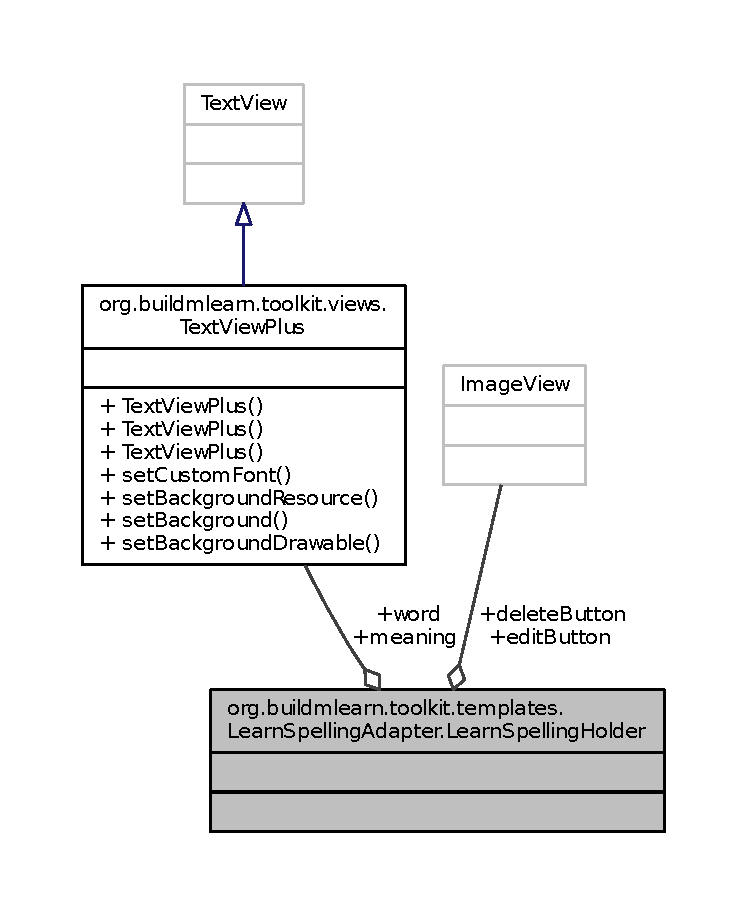
\includegraphics[width=350pt]{d4/df5/classorg_1_1buildmlearn_1_1toolkit_1_1templates_1_1LearnSpellingAdapter_1_1LearnSpellingHolder__coll__graph}
\end{center}
\end{figure}
\subsection*{Public Attributes}
\begin{DoxyCompactItemize}
\item 
\hyperlink{classorg_1_1buildmlearn_1_1toolkit_1_1views_1_1TextViewPlus}{Text\-View\-Plus} \hyperlink{classorg_1_1buildmlearn_1_1toolkit_1_1templates_1_1LearnSpellingAdapter_1_1LearnSpellingHolder_a6e8838ae9bf29b6005fe9fff6a174e77}{word}
\item 
\hyperlink{classorg_1_1buildmlearn_1_1toolkit_1_1views_1_1TextViewPlus}{Text\-View\-Plus} \hyperlink{classorg_1_1buildmlearn_1_1toolkit_1_1templates_1_1LearnSpellingAdapter_1_1LearnSpellingHolder_afbe6d699245b23d551f1bf5105e842a6}{meaning}
\item 
Image\-View \hyperlink{classorg_1_1buildmlearn_1_1toolkit_1_1templates_1_1LearnSpellingAdapter_1_1LearnSpellingHolder_a5db8d3295fb4eee7a87b536b32ad4082}{edit\-Button}
\item 
Image\-View \hyperlink{classorg_1_1buildmlearn_1_1toolkit_1_1templates_1_1LearnSpellingAdapter_1_1LearnSpellingHolder_a89783eb886d6820d344f9e3e3075480a}{delete\-Button}
\end{DoxyCompactItemize}


\subsection{Member Data Documentation}
\hypertarget{classorg_1_1buildmlearn_1_1toolkit_1_1templates_1_1LearnSpellingAdapter_1_1LearnSpellingHolder_a89783eb886d6820d344f9e3e3075480a}{\index{org\-::buildmlearn\-::toolkit\-::templates\-::\-Learn\-Spelling\-Adapter\-::\-Learn\-Spelling\-Holder@{org\-::buildmlearn\-::toolkit\-::templates\-::\-Learn\-Spelling\-Adapter\-::\-Learn\-Spelling\-Holder}!delete\-Button@{delete\-Button}}
\index{delete\-Button@{delete\-Button}!org::buildmlearn::toolkit::templates::LearnSpellingAdapter::LearnSpellingHolder@{org\-::buildmlearn\-::toolkit\-::templates\-::\-Learn\-Spelling\-Adapter\-::\-Learn\-Spelling\-Holder}}
\subsubsection[{delete\-Button}]{\setlength{\rightskip}{0pt plus 5cm}Image\-View org.\-buildmlearn.\-toolkit.\-templates.\-Learn\-Spelling\-Adapter.\-Learn\-Spelling\-Holder.\-delete\-Button}}\label{classorg_1_1buildmlearn_1_1toolkit_1_1templates_1_1LearnSpellingAdapter_1_1LearnSpellingHolder_a89783eb886d6820d344f9e3e3075480a}
\hypertarget{classorg_1_1buildmlearn_1_1toolkit_1_1templates_1_1LearnSpellingAdapter_1_1LearnSpellingHolder_a5db8d3295fb4eee7a87b536b32ad4082}{\index{org\-::buildmlearn\-::toolkit\-::templates\-::\-Learn\-Spelling\-Adapter\-::\-Learn\-Spelling\-Holder@{org\-::buildmlearn\-::toolkit\-::templates\-::\-Learn\-Spelling\-Adapter\-::\-Learn\-Spelling\-Holder}!edit\-Button@{edit\-Button}}
\index{edit\-Button@{edit\-Button}!org::buildmlearn::toolkit::templates::LearnSpellingAdapter::LearnSpellingHolder@{org\-::buildmlearn\-::toolkit\-::templates\-::\-Learn\-Spelling\-Adapter\-::\-Learn\-Spelling\-Holder}}
\subsubsection[{edit\-Button}]{\setlength{\rightskip}{0pt plus 5cm}Image\-View org.\-buildmlearn.\-toolkit.\-templates.\-Learn\-Spelling\-Adapter.\-Learn\-Spelling\-Holder.\-edit\-Button}}\label{classorg_1_1buildmlearn_1_1toolkit_1_1templates_1_1LearnSpellingAdapter_1_1LearnSpellingHolder_a5db8d3295fb4eee7a87b536b32ad4082}
\hypertarget{classorg_1_1buildmlearn_1_1toolkit_1_1templates_1_1LearnSpellingAdapter_1_1LearnSpellingHolder_afbe6d699245b23d551f1bf5105e842a6}{\index{org\-::buildmlearn\-::toolkit\-::templates\-::\-Learn\-Spelling\-Adapter\-::\-Learn\-Spelling\-Holder@{org\-::buildmlearn\-::toolkit\-::templates\-::\-Learn\-Spelling\-Adapter\-::\-Learn\-Spelling\-Holder}!meaning@{meaning}}
\index{meaning@{meaning}!org::buildmlearn::toolkit::templates::LearnSpellingAdapter::LearnSpellingHolder@{org\-::buildmlearn\-::toolkit\-::templates\-::\-Learn\-Spelling\-Adapter\-::\-Learn\-Spelling\-Holder}}
\subsubsection[{meaning}]{\setlength{\rightskip}{0pt plus 5cm}{\bf Text\-View\-Plus} org.\-buildmlearn.\-toolkit.\-templates.\-Learn\-Spelling\-Adapter.\-Learn\-Spelling\-Holder.\-meaning}}\label{classorg_1_1buildmlearn_1_1toolkit_1_1templates_1_1LearnSpellingAdapter_1_1LearnSpellingHolder_afbe6d699245b23d551f1bf5105e842a6}
\hypertarget{classorg_1_1buildmlearn_1_1toolkit_1_1templates_1_1LearnSpellingAdapter_1_1LearnSpellingHolder_a6e8838ae9bf29b6005fe9fff6a174e77}{\index{org\-::buildmlearn\-::toolkit\-::templates\-::\-Learn\-Spelling\-Adapter\-::\-Learn\-Spelling\-Holder@{org\-::buildmlearn\-::toolkit\-::templates\-::\-Learn\-Spelling\-Adapter\-::\-Learn\-Spelling\-Holder}!word@{word}}
\index{word@{word}!org::buildmlearn::toolkit::templates::LearnSpellingAdapter::LearnSpellingHolder@{org\-::buildmlearn\-::toolkit\-::templates\-::\-Learn\-Spelling\-Adapter\-::\-Learn\-Spelling\-Holder}}
\subsubsection[{word}]{\setlength{\rightskip}{0pt plus 5cm}{\bf Text\-View\-Plus} org.\-buildmlearn.\-toolkit.\-templates.\-Learn\-Spelling\-Adapter.\-Learn\-Spelling\-Holder.\-word}}\label{classorg_1_1buildmlearn_1_1toolkit_1_1templates_1_1LearnSpellingAdapter_1_1LearnSpellingHolder_a6e8838ae9bf29b6005fe9fff6a174e77}


The documentation for this class was generated from the following file\-:\begin{DoxyCompactItemize}
\item 
/\-Buildm\-Learn-\/\-Toolkit-\/\-Android/source-\/code/app/src/main/java/org/buildmlearn/toolkit/templates/\hyperlink{LearnSpellingAdapter_8java}{Learn\-Spelling\-Adapter.\-java}\end{DoxyCompactItemize}

\hypertarget{classorg_1_1buildmlearn_1_1toolkit_1_1templates_1_1LearnSpellingModel}{\section{org.\-buildmlearn.\-toolkit.\-templates.\-Learn\-Spelling\-Model Class Reference}
\label{classorg_1_1buildmlearn_1_1toolkit_1_1templates_1_1LearnSpellingModel}\index{org.\-buildmlearn.\-toolkit.\-templates.\-Learn\-Spelling\-Model@{org.\-buildmlearn.\-toolkit.\-templates.\-Learn\-Spelling\-Model}}
}


Model class for Learn Spelling Template Editor data.  




Inheritance diagram for org.\-buildmlearn.\-toolkit.\-templates.\-Learn\-Spelling\-Model\-:
\nopagebreak
\begin{figure}[H]
\begin{center}
\leavevmode
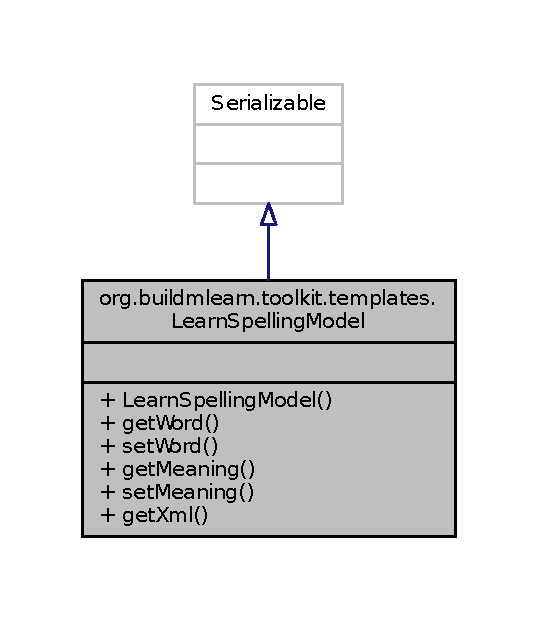
\includegraphics[width=258pt]{d7/de3/classorg_1_1buildmlearn_1_1toolkit_1_1templates_1_1LearnSpellingModel__inherit__graph}
\end{center}
\end{figure}


Collaboration diagram for org.\-buildmlearn.\-toolkit.\-templates.\-Learn\-Spelling\-Model\-:
\nopagebreak
\begin{figure}[H]
\begin{center}
\leavevmode
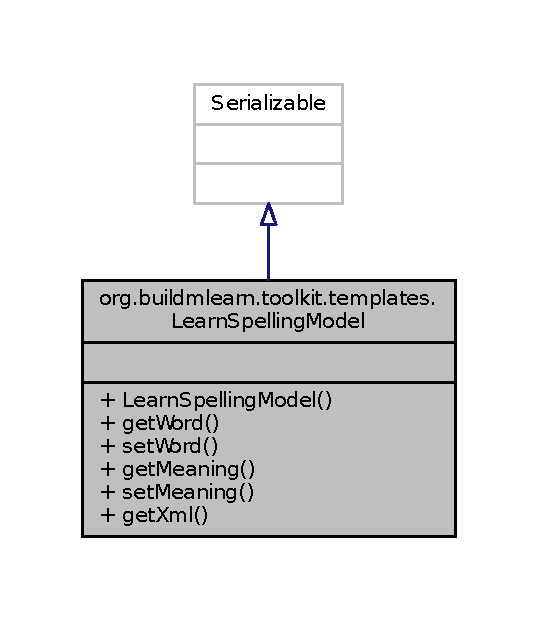
\includegraphics[width=258pt]{de/d04/classorg_1_1buildmlearn_1_1toolkit_1_1templates_1_1LearnSpellingModel__coll__graph}
\end{center}
\end{figure}
\subsection*{Public Member Functions}
\begin{DoxyCompactItemize}
\item 
\hyperlink{classorg_1_1buildmlearn_1_1toolkit_1_1templates_1_1LearnSpellingModel_a3a4f0e6afa5518b6eee58e848921158c}{Learn\-Spelling\-Model} (String info\-Object, String meaning)
\item 
String \hyperlink{classorg_1_1buildmlearn_1_1toolkit_1_1templates_1_1LearnSpellingModel_a076fc8889dd81620c579511cf84cd526}{get\-Word} ()
\item 
void \hyperlink{classorg_1_1buildmlearn_1_1toolkit_1_1templates_1_1LearnSpellingModel_a19e23525a8849fc802aa12ab90f511a2}{set\-Word} (String word)
\item 
String \hyperlink{classorg_1_1buildmlearn_1_1toolkit_1_1templates_1_1LearnSpellingModel_a74785e99070999af859d2211d465d0a2}{get\-Meaning} ()
\item 
void \hyperlink{classorg_1_1buildmlearn_1_1toolkit_1_1templates_1_1LearnSpellingModel_a8e34f3d996440542557e0352429906f2}{set\-Meaning} (String meaning)
\item 
Element \hyperlink{classorg_1_1buildmlearn_1_1toolkit_1_1templates_1_1LearnSpellingModel_a17c942dd683427e078dae596fbf9972a}{get\-Xml} (Document doc)
\end{DoxyCompactItemize}


\subsection{Detailed Description}
Model class for Learn Spelling Template Editor data. 

Created by abhishek on 17/06/15 at 9\-:49 P\-M. 

\subsection{Constructor \& Destructor Documentation}
\hypertarget{classorg_1_1buildmlearn_1_1toolkit_1_1templates_1_1LearnSpellingModel_a3a4f0e6afa5518b6eee58e848921158c}{\index{org\-::buildmlearn\-::toolkit\-::templates\-::\-Learn\-Spelling\-Model@{org\-::buildmlearn\-::toolkit\-::templates\-::\-Learn\-Spelling\-Model}!Learn\-Spelling\-Model@{Learn\-Spelling\-Model}}
\index{Learn\-Spelling\-Model@{Learn\-Spelling\-Model}!org::buildmlearn::toolkit::templates::LearnSpellingModel@{org\-::buildmlearn\-::toolkit\-::templates\-::\-Learn\-Spelling\-Model}}
\subsubsection[{Learn\-Spelling\-Model}]{\setlength{\rightskip}{0pt plus 5cm}org.\-buildmlearn.\-toolkit.\-templates.\-Learn\-Spelling\-Model.\-Learn\-Spelling\-Model (
\begin{DoxyParamCaption}
\item[{String}]{info\-Object, }
\item[{String}]{meaning}
\end{DoxyParamCaption}
)}}\label{classorg_1_1buildmlearn_1_1toolkit_1_1templates_1_1LearnSpellingModel_a3a4f0e6afa5518b6eee58e848921158c}

\begin{DoxyCode}
18                                                                  \{
19         this.mWord = infoObject;
20         this.mMeaning = meaning;
21     \}
\end{DoxyCode}


\subsection{Member Function Documentation}
\hypertarget{classorg_1_1buildmlearn_1_1toolkit_1_1templates_1_1LearnSpellingModel_a74785e99070999af859d2211d465d0a2}{\index{org\-::buildmlearn\-::toolkit\-::templates\-::\-Learn\-Spelling\-Model@{org\-::buildmlearn\-::toolkit\-::templates\-::\-Learn\-Spelling\-Model}!get\-Meaning@{get\-Meaning}}
\index{get\-Meaning@{get\-Meaning}!org::buildmlearn::toolkit::templates::LearnSpellingModel@{org\-::buildmlearn\-::toolkit\-::templates\-::\-Learn\-Spelling\-Model}}
\subsubsection[{get\-Meaning}]{\setlength{\rightskip}{0pt plus 5cm}String org.\-buildmlearn.\-toolkit.\-templates.\-Learn\-Spelling\-Model.\-get\-Meaning (
\begin{DoxyParamCaption}
{}
\end{DoxyParamCaption}
)}}\label{classorg_1_1buildmlearn_1_1toolkit_1_1templates_1_1LearnSpellingModel_a74785e99070999af859d2211d465d0a2}

\begin{DoxyCode}
31                                \{
32         \textcolor{keywordflow}{return} mMeaning;
33     \}
\end{DoxyCode}
\hypertarget{classorg_1_1buildmlearn_1_1toolkit_1_1templates_1_1LearnSpellingModel_a076fc8889dd81620c579511cf84cd526}{\index{org\-::buildmlearn\-::toolkit\-::templates\-::\-Learn\-Spelling\-Model@{org\-::buildmlearn\-::toolkit\-::templates\-::\-Learn\-Spelling\-Model}!get\-Word@{get\-Word}}
\index{get\-Word@{get\-Word}!org::buildmlearn::toolkit::templates::LearnSpellingModel@{org\-::buildmlearn\-::toolkit\-::templates\-::\-Learn\-Spelling\-Model}}
\subsubsection[{get\-Word}]{\setlength{\rightskip}{0pt plus 5cm}String org.\-buildmlearn.\-toolkit.\-templates.\-Learn\-Spelling\-Model.\-get\-Word (
\begin{DoxyParamCaption}
{}
\end{DoxyParamCaption}
)}}\label{classorg_1_1buildmlearn_1_1toolkit_1_1templates_1_1LearnSpellingModel_a076fc8889dd81620c579511cf84cd526}

\begin{DoxyCode}
23                             \{
24         \textcolor{keywordflow}{return} mWord;
25     \}
\end{DoxyCode}
\hypertarget{classorg_1_1buildmlearn_1_1toolkit_1_1templates_1_1LearnSpellingModel_a17c942dd683427e078dae596fbf9972a}{\index{org\-::buildmlearn\-::toolkit\-::templates\-::\-Learn\-Spelling\-Model@{org\-::buildmlearn\-::toolkit\-::templates\-::\-Learn\-Spelling\-Model}!get\-Xml@{get\-Xml}}
\index{get\-Xml@{get\-Xml}!org::buildmlearn::toolkit::templates::LearnSpellingModel@{org\-::buildmlearn\-::toolkit\-::templates\-::\-Learn\-Spelling\-Model}}
\subsubsection[{get\-Xml}]{\setlength{\rightskip}{0pt plus 5cm}Element org.\-buildmlearn.\-toolkit.\-templates.\-Learn\-Spelling\-Model.\-get\-Xml (
\begin{DoxyParamCaption}
\item[{Document}]{doc}
\end{DoxyParamCaption}
)}}\label{classorg_1_1buildmlearn_1_1toolkit_1_1templates_1_1LearnSpellingModel_a17c942dd683427e078dae596fbf9972a}

\begin{DoxyCode}
39                                         \{
40         Element rootElement = doc.createElement(\textcolor{stringliteral}{"item"});
41         Element questionElement = doc.createElement(\textcolor{stringliteral}{"word"});
42         questionElement.appendChild(doc.createTextNode(mWord));
43         rootElement.appendChild(questionElement);
44         Element answerElement = doc.createElement(\textcolor{stringliteral}{"meaning"});
45         answerElement.appendChild(doc.createTextNode(String.valueOf(mMeaning)));
46         rootElement.appendChild(answerElement);
47         \textcolor{keywordflow}{return} rootElement;
48     \}
\end{DoxyCode}
\hypertarget{classorg_1_1buildmlearn_1_1toolkit_1_1templates_1_1LearnSpellingModel_a8e34f3d996440542557e0352429906f2}{\index{org\-::buildmlearn\-::toolkit\-::templates\-::\-Learn\-Spelling\-Model@{org\-::buildmlearn\-::toolkit\-::templates\-::\-Learn\-Spelling\-Model}!set\-Meaning@{set\-Meaning}}
\index{set\-Meaning@{set\-Meaning}!org::buildmlearn::toolkit::templates::LearnSpellingModel@{org\-::buildmlearn\-::toolkit\-::templates\-::\-Learn\-Spelling\-Model}}
\subsubsection[{set\-Meaning}]{\setlength{\rightskip}{0pt plus 5cm}void org.\-buildmlearn.\-toolkit.\-templates.\-Learn\-Spelling\-Model.\-set\-Meaning (
\begin{DoxyParamCaption}
\item[{String}]{meaning}
\end{DoxyParamCaption}
)}}\label{classorg_1_1buildmlearn_1_1toolkit_1_1templates_1_1LearnSpellingModel_a8e34f3d996440542557e0352429906f2}

\begin{DoxyCode}
35                                            \{
36         this.mMeaning = meaning;
37     \}
\end{DoxyCode}
\hypertarget{classorg_1_1buildmlearn_1_1toolkit_1_1templates_1_1LearnSpellingModel_a19e23525a8849fc802aa12ab90f511a2}{\index{org\-::buildmlearn\-::toolkit\-::templates\-::\-Learn\-Spelling\-Model@{org\-::buildmlearn\-::toolkit\-::templates\-::\-Learn\-Spelling\-Model}!set\-Word@{set\-Word}}
\index{set\-Word@{set\-Word}!org::buildmlearn::toolkit::templates::LearnSpellingModel@{org\-::buildmlearn\-::toolkit\-::templates\-::\-Learn\-Spelling\-Model}}
\subsubsection[{set\-Word}]{\setlength{\rightskip}{0pt plus 5cm}void org.\-buildmlearn.\-toolkit.\-templates.\-Learn\-Spelling\-Model.\-set\-Word (
\begin{DoxyParamCaption}
\item[{String}]{word}
\end{DoxyParamCaption}
)}}\label{classorg_1_1buildmlearn_1_1toolkit_1_1templates_1_1LearnSpellingModel_a19e23525a8849fc802aa12ab90f511a2}

\begin{DoxyCode}
27                                      \{
28         this.mWord = word;
29     \}
\end{DoxyCode}


The documentation for this class was generated from the following file\-:\begin{DoxyCompactItemize}
\item 
/\-Buildm\-Learn-\/\-Toolkit-\/\-Android/source-\/code/app/src/main/java/org/buildmlearn/toolkit/templates/\hyperlink{LearnSpellingModel_8java}{Learn\-Spelling\-Model.\-java}\end{DoxyCompactItemize}

\hypertarget{classorg_1_1buildmlearn_1_1toolkit_1_1templates_1_1LearnSpellingTemplate}{\section{org.\-buildmlearn.\-toolkit.\-templates.\-Learn\-Spelling\-Template Class Reference}
\label{classorg_1_1buildmlearn_1_1toolkit_1_1templates_1_1LearnSpellingTemplate}\index{org.\-buildmlearn.\-toolkit.\-templates.\-Learn\-Spelling\-Template@{org.\-buildmlearn.\-toolkit.\-templates.\-Learn\-Spelling\-Template}}
}


Learn Spelling template code implementing methods of Template\-Interface.  




Inheritance diagram for org.\-buildmlearn.\-toolkit.\-templates.\-Learn\-Spelling\-Template\-:
\nopagebreak
\begin{figure}[H]
\begin{center}
\leavevmode
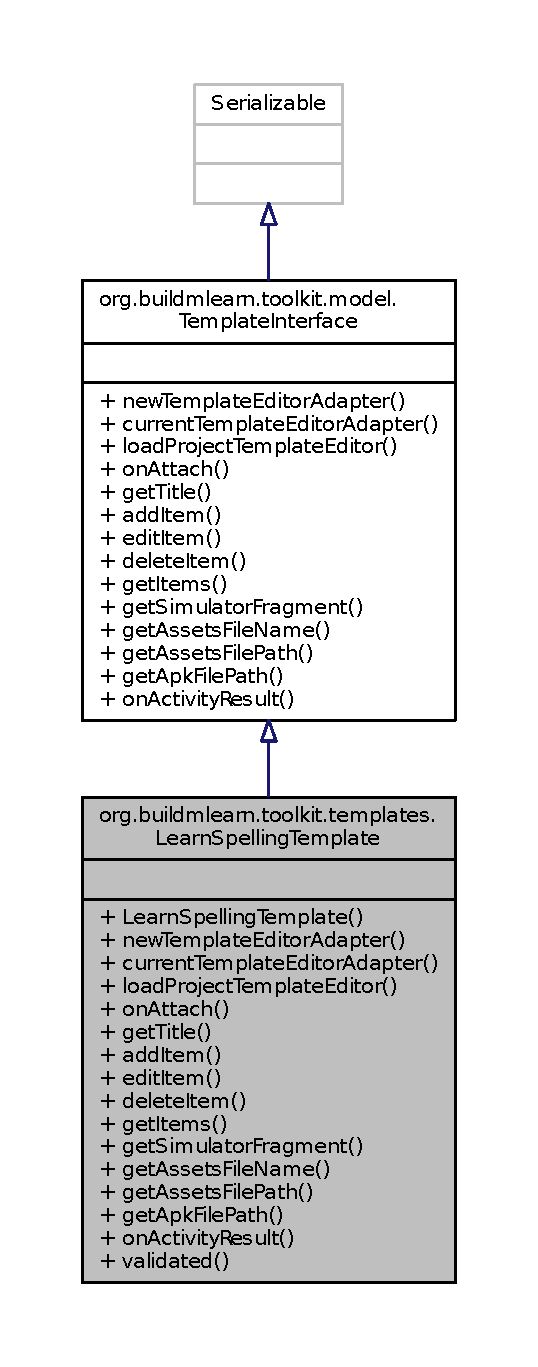
\includegraphics[height=550pt]{d1/da1/classorg_1_1buildmlearn_1_1toolkit_1_1templates_1_1LearnSpellingTemplate__inherit__graph}
\end{center}
\end{figure}


Collaboration diagram for org.\-buildmlearn.\-toolkit.\-templates.\-Learn\-Spelling\-Template\-:
\nopagebreak
\begin{figure}[H]
\begin{center}
\leavevmode
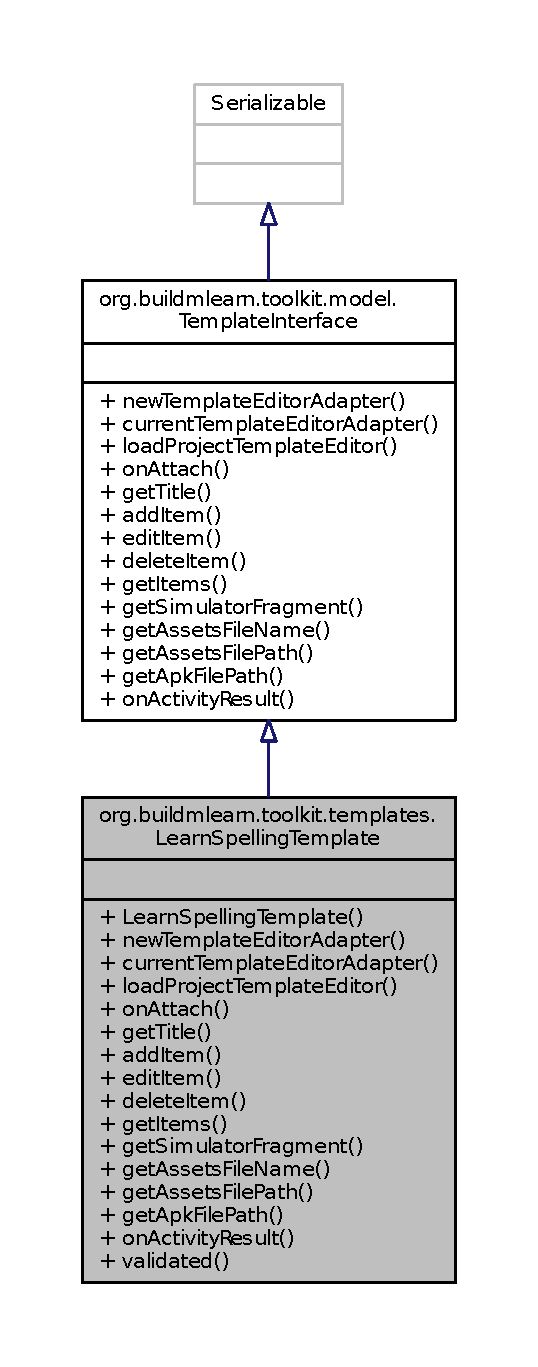
\includegraphics[height=550pt]{d2/d14/classorg_1_1buildmlearn_1_1toolkit_1_1templates_1_1LearnSpellingTemplate__coll__graph}
\end{center}
\end{figure}
\subsection*{Public Member Functions}
\begin{DoxyCompactItemize}
\item 
\hyperlink{classorg_1_1buildmlearn_1_1toolkit_1_1templates_1_1LearnSpellingTemplate_a09607c7a192a1e5754bfe51d3cac5df9}{Learn\-Spelling\-Template} ()
\item 
Base\-Adapter \hyperlink{classorg_1_1buildmlearn_1_1toolkit_1_1templates_1_1LearnSpellingTemplate_a532c1020ba161742148024ce7346d306}{new\-Template\-Editor\-Adapter} (Context context)
\begin{DoxyCompactList}\small\item\em Called from Template Editor when template editor is started for creating a new template project. \end{DoxyCompactList}\item 
Base\-Adapter \hyperlink{classorg_1_1buildmlearn_1_1toolkit_1_1templates_1_1LearnSpellingTemplate_a46ba1da1d9832f8e2ffbaf5a416a23f8}{current\-Template\-Editor\-Adapter} ()
\begin{DoxyCompactList}\small\item\em This function is used to get the adapter (containing template data) for a existing/current template project. \end{DoxyCompactList}\item 
Base\-Adapter \hyperlink{classorg_1_1buildmlearn_1_1toolkit_1_1templates_1_1LearnSpellingTemplate_a889d8d414440285b80ca93b6a243e05e}{load\-Project\-Template\-Editor} (Context context, Array\-List$<$ Element $>$ data)
\item 
String \hyperlink{classorg_1_1buildmlearn_1_1toolkit_1_1templates_1_1LearnSpellingTemplate_ab644415ca83560eecd107a9d2a22e65b}{on\-Attach} ()
\begin{DoxyCompactList}\small\item\em Called from Template\-Editor whenever a template is attached to Template\-Editor. \end{DoxyCompactList}\item 
String \hyperlink{classorg_1_1buildmlearn_1_1toolkit_1_1templates_1_1LearnSpellingTemplate_a06f51659532ed7300478ad233aa3e8b7}{get\-Title} ()
\begin{DoxyCompactList}\small\item\em Used to get the title of the templaye. Mainly used to update Action\-Bar in Template Editor. \end{DoxyCompactList}\item 
void \hyperlink{classorg_1_1buildmlearn_1_1toolkit_1_1templates_1_1LearnSpellingTemplate_a79df95c6c1990205f55cbc75a0b9a163}{add\-Item} (final Activity activity)
\item 
void \hyperlink{classorg_1_1buildmlearn_1_1toolkit_1_1templates_1_1LearnSpellingTemplate_ac1a2b3a4507302be292deb019ab563f4}{edit\-Item} (final Activity activity, int position)
\item 
void \hyperlink{classorg_1_1buildmlearn_1_1toolkit_1_1templates_1_1LearnSpellingTemplate_ad8f1904727ddd68bc429ae85fd916a1c}{delete\-Item} (int position)
\begin{DoxyCompactList}\small\item\em Remove an item form template data list. \end{DoxyCompactList}\item 
Array\-List$<$ Element $>$ \hyperlink{classorg_1_1buildmlearn_1_1toolkit_1_1templates_1_1LearnSpellingTemplate_a289b6e6a43daae52a975f3e74c03fa97}{get\-Items} (Document doc)
\item 
Fragment \hyperlink{classorg_1_1buildmlearn_1_1toolkit_1_1templates_1_1LearnSpellingTemplate_acf73238fe4aed0e287fd3151e6a2f653}{get\-Simulator\-Fragment} (String file\-Path\-With\-Name)
\begin{DoxyCompactList}\small\item\em Returns a fragment required for the Simulator Activity. \end{DoxyCompactList}\item 
String \hyperlink{classorg_1_1buildmlearn_1_1toolkit_1_1templates_1_1LearnSpellingTemplate_a17e1b99d6ac68e1912ea00bb29e368bc}{get\-Assets\-File\-Name} ()
\begin{DoxyCompactList}\small\item\em Name of the xml file congaing template data in the assets folders in the build apk. \end{DoxyCompactList}\item 
String \hyperlink{classorg_1_1buildmlearn_1_1toolkit_1_1templates_1_1LearnSpellingTemplate_a49bf35434b6abe45d04db8ed1f16b9e1}{get\-Assets\-File\-Path} ()
\begin{DoxyCompactList}\small\item\em Folder path in which the apk is stored in the build A\-P\-K. \end{DoxyCompactList}\item 
String \hyperlink{classorg_1_1buildmlearn_1_1toolkit_1_1templates_1_1LearnSpellingTemplate_a05c6bdea670350a1f2aed2c9c4b28e10}{get\-Apk\-File\-Path} ()
\item 
void \hyperlink{classorg_1_1buildmlearn_1_1toolkit_1_1templates_1_1LearnSpellingTemplate_a3717f8c402a9da264b3d8e6665532c3c}{on\-Activity\-Result} (Context context, int request\-Code, int result\-Code, Intent intent)
\begin{DoxyCompactList}\small\item\em Called whenever on\-Activity\-Result is called in Template Editor. Can be used to perform action related to intent and callbacks. \end{DoxyCompactList}\end{DoxyCompactItemize}
\subsection*{Static Public Member Functions}
\begin{DoxyCompactItemize}
\item 
static boolean \hyperlink{classorg_1_1buildmlearn_1_1toolkit_1_1templates_1_1LearnSpellingTemplate_a5acea6370884485ccc57d4068ec43a24}{validated} (Context context, Edit\-Text word, Edit\-Text meaning)
\end{DoxyCompactItemize}


\subsection{Detailed Description}
Learn Spelling template code implementing methods of Template\-Interface. 

Created by abhishek on 16/06/15 at 9\-:59 P\-M. 

\subsection{Constructor \& Destructor Documentation}
\hypertarget{classorg_1_1buildmlearn_1_1toolkit_1_1templates_1_1LearnSpellingTemplate_a09607c7a192a1e5754bfe51d3cac5df9}{\index{org\-::buildmlearn\-::toolkit\-::templates\-::\-Learn\-Spelling\-Template@{org\-::buildmlearn\-::toolkit\-::templates\-::\-Learn\-Spelling\-Template}!Learn\-Spelling\-Template@{Learn\-Spelling\-Template}}
\index{Learn\-Spelling\-Template@{Learn\-Spelling\-Template}!org::buildmlearn::toolkit::templates::LearnSpellingTemplate@{org\-::buildmlearn\-::toolkit\-::templates\-::\-Learn\-Spelling\-Template}}
\subsubsection[{Learn\-Spelling\-Template}]{\setlength{\rightskip}{0pt plus 5cm}org.\-buildmlearn.\-toolkit.\-templates.\-Learn\-Spelling\-Template.\-Learn\-Spelling\-Template (
\begin{DoxyParamCaption}
{}
\end{DoxyParamCaption}
)}}\label{classorg_1_1buildmlearn_1_1toolkit_1_1templates_1_1LearnSpellingTemplate_a09607c7a192a1e5754bfe51d3cac5df9}

\begin{DoxyCode}
33                                    \{
34         mLearnSpellingData = \textcolor{keyword}{new} ArrayList<>();
35     \}
\end{DoxyCode}


\subsection{Member Function Documentation}
\hypertarget{classorg_1_1buildmlearn_1_1toolkit_1_1templates_1_1LearnSpellingTemplate_a79df95c6c1990205f55cbc75a0b9a163}{\index{org\-::buildmlearn\-::toolkit\-::templates\-::\-Learn\-Spelling\-Template@{org\-::buildmlearn\-::toolkit\-::templates\-::\-Learn\-Spelling\-Template}!add\-Item@{add\-Item}}
\index{add\-Item@{add\-Item}!org::buildmlearn::toolkit::templates::LearnSpellingTemplate@{org\-::buildmlearn\-::toolkit\-::templates\-::\-Learn\-Spelling\-Template}}
\subsubsection[{add\-Item}]{\setlength{\rightskip}{0pt plus 5cm}void org.\-buildmlearn.\-toolkit.\-templates.\-Learn\-Spelling\-Template.\-add\-Item (
\begin{DoxyParamCaption}
\item[{final Activity}]{activity}
\end{DoxyParamCaption}
)}}\label{classorg_1_1buildmlearn_1_1toolkit_1_1templates_1_1LearnSpellingTemplate_a79df95c6c1990205f55cbc75a0b9a163}

\begin{DoxyCode}
90                                                  \{
91 
92         \textcolor{keyword}{final} MaterialDialog dialog = \textcolor{keyword}{new} MaterialDialog.Builder(activity)
93                 .title(R.string.info\_add\_new\_title)
94                 .customView(R.layout.info\_dialog\_add\_edit\_data, \textcolor{keyword}{true})
95                 .positiveText(R.string.info\_template\_add)
96                 .negativeText(R.string.info\_template\_delete)
97                 .build();
98 
99         \textcolor{keyword}{final} EditText word = (EditText) dialog.findViewById(R.id.info\_word);
100         \textcolor{keyword}{final} EditText meaning = (EditText) dialog.findViewById(R.id.info\_meaning);
101 
102         dialog.getActionButton(DialogAction.POSITIVE).setOnClickListener(\textcolor{keyword}{new} View.OnClickListener() \{
103             @Override
104             \textcolor{keyword}{public} \textcolor{keywordtype}{void} onClick(View v) \{
105 
106                 \textcolor{keywordflow}{if} (\hyperlink{classorg_1_1buildmlearn_1_1toolkit_1_1templates_1_1LearnSpellingTemplate_a5acea6370884485ccc57d4068ec43a24}{validated}(activity, word, meaning)) \{
107                     String wordText = word.getText().toString();
108                     String meaningText = meaning.getText().toString();
109 
110                     LearnSpellingModel temp = \textcolor{keyword}{new} LearnSpellingModel(wordText, meaningText);
111                     mLearnSpellingData.add(temp);
112                     adapter.notifyDataSetChanged();
113                     dialog.dismiss();
114                 \}
115 
116             \}
117         \});
118 
119         dialog.show();
120 
121     \}
\end{DoxyCode}
\hypertarget{classorg_1_1buildmlearn_1_1toolkit_1_1templates_1_1LearnSpellingTemplate_a46ba1da1d9832f8e2ffbaf5a416a23f8}{\index{org\-::buildmlearn\-::toolkit\-::templates\-::\-Learn\-Spelling\-Template@{org\-::buildmlearn\-::toolkit\-::templates\-::\-Learn\-Spelling\-Template}!current\-Template\-Editor\-Adapter@{current\-Template\-Editor\-Adapter}}
\index{current\-Template\-Editor\-Adapter@{current\-Template\-Editor\-Adapter}!org::buildmlearn::toolkit::templates::LearnSpellingTemplate@{org\-::buildmlearn\-::toolkit\-::templates\-::\-Learn\-Spelling\-Template}}
\subsubsection[{current\-Template\-Editor\-Adapter}]{\setlength{\rightskip}{0pt plus 5cm}Base\-Adapter org.\-buildmlearn.\-toolkit.\-templates.\-Learn\-Spelling\-Template.\-current\-Template\-Editor\-Adapter (
\begin{DoxyParamCaption}
{}
\end{DoxyParamCaption}
)}}\label{classorg_1_1buildmlearn_1_1toolkit_1_1templates_1_1LearnSpellingTemplate_a46ba1da1d9832f8e2ffbaf5a416a23f8}


This function is used to get the adapter (containing template data) for a existing/current template project. 

\begin{DoxyReturn}{Returns}
Base\-Adapter inherited Object 
\end{DoxyReturn}


Implements \hyperlink{interfaceorg_1_1buildmlearn_1_1toolkit_1_1model_1_1TemplateInterface_ae433eedc291006e78b65b0fc4135d560}{org.\-buildmlearn.\-toolkit.\-model.\-Template\-Interface}.


\begin{DoxyCode}
63                                                       \{
64         \textcolor{keywordflow}{return} adapter;
65     \}
\end{DoxyCode}
\hypertarget{classorg_1_1buildmlearn_1_1toolkit_1_1templates_1_1LearnSpellingTemplate_ad8f1904727ddd68bc429ae85fd916a1c}{\index{org\-::buildmlearn\-::toolkit\-::templates\-::\-Learn\-Spelling\-Template@{org\-::buildmlearn\-::toolkit\-::templates\-::\-Learn\-Spelling\-Template}!delete\-Item@{delete\-Item}}
\index{delete\-Item@{delete\-Item}!org::buildmlearn::toolkit::templates::LearnSpellingTemplate@{org\-::buildmlearn\-::toolkit\-::templates\-::\-Learn\-Spelling\-Template}}
\subsubsection[{delete\-Item}]{\setlength{\rightskip}{0pt plus 5cm}void org.\-buildmlearn.\-toolkit.\-templates.\-Learn\-Spelling\-Template.\-delete\-Item (
\begin{DoxyParamCaption}
\item[{int}]{position}
\end{DoxyParamCaption}
)}}\label{classorg_1_1buildmlearn_1_1toolkit_1_1templates_1_1LearnSpellingTemplate_ad8f1904727ddd68bc429ae85fd916a1c}


Remove an item form template data list. 


\begin{DoxyParams}{Parameters}
{\em position} & Position of the item to be removed \\
\hline
\end{DoxyParams}


Implements \hyperlink{interfaceorg_1_1buildmlearn_1_1toolkit_1_1model_1_1TemplateInterface_aeb65a5ef72b939c20b24cd7c02a80a97}{org.\-buildmlearn.\-toolkit.\-model.\-Template\-Interface}.


\begin{DoxyCode}
162                                          \{
163 
164 
165         mLearnSpellingData.remove(position);
166         adapter.notifyDataSetChanged();
167 
168     \}
\end{DoxyCode}
\hypertarget{classorg_1_1buildmlearn_1_1toolkit_1_1templates_1_1LearnSpellingTemplate_ac1a2b3a4507302be292deb019ab563f4}{\index{org\-::buildmlearn\-::toolkit\-::templates\-::\-Learn\-Spelling\-Template@{org\-::buildmlearn\-::toolkit\-::templates\-::\-Learn\-Spelling\-Template}!edit\-Item@{edit\-Item}}
\index{edit\-Item@{edit\-Item}!org::buildmlearn::toolkit::templates::LearnSpellingTemplate@{org\-::buildmlearn\-::toolkit\-::templates\-::\-Learn\-Spelling\-Template}}
\subsubsection[{edit\-Item}]{\setlength{\rightskip}{0pt plus 5cm}void org.\-buildmlearn.\-toolkit.\-templates.\-Learn\-Spelling\-Template.\-edit\-Item (
\begin{DoxyParamCaption}
\item[{final Activity}]{activity, }
\item[{int}]{position}
\end{DoxyParamCaption}
)}}\label{classorg_1_1buildmlearn_1_1toolkit_1_1templates_1_1LearnSpellingTemplate_ac1a2b3a4507302be292deb019ab563f4}

\begin{DoxyCode}
124                                                                 \{
125         \textcolor{keyword}{final} MaterialDialog dialog = \textcolor{keyword}{new} MaterialDialog.Builder(activity)
126                 .title(R.string.info\_add\_new\_title)
127                 .customView(R.layout.info\_dialog\_add\_edit\_data, \textcolor{keyword}{true})
128                 .positiveText(R.string.info\_template\_add)
129                 .negativeText(R.string.info\_template\_delete)
130                 .build();
131 
132         \textcolor{keyword}{final} LearnSpellingModel data = mLearnSpellingData.get(position);
133 
134         \textcolor{keyword}{final} EditText word = (EditText) dialog.findViewById(R.id.info\_word);
135         \textcolor{keyword}{final} EditText meaning = (EditText) dialog.findViewById(R.id.info\_meaning);
136         word.setText(data.getWord());
137         meaning.setText(data.getMeaning());
138 
139         dialog.getActionButton(DialogAction.POSITIVE).setOnClickListener(\textcolor{keyword}{new} View.OnClickListener() \{
140             @Override
141             \textcolor{keyword}{public} \textcolor{keywordtype}{void} onClick(View v) \{
142 
143                 \textcolor{keywordflow}{if} (\hyperlink{classorg_1_1buildmlearn_1_1toolkit_1_1templates_1_1LearnSpellingTemplate_a5acea6370884485ccc57d4068ec43a24}{validated}(activity, word, meaning)) \{
144                     String wordText = word.getText().toString();
145                     String meaningText = meaning.getText().toString();
146 
147                     data.setWord(wordText);
148                     data.setMeaning(meaningText);
149 
150                     adapter.notifyDataSetChanged();
151                     dialog.dismiss();
152                 \}
153 
154             \}
155         \});
156 
157         dialog.show();
158 
159     \}
\end{DoxyCode}
\hypertarget{classorg_1_1buildmlearn_1_1toolkit_1_1templates_1_1LearnSpellingTemplate_a05c6bdea670350a1f2aed2c9c4b28e10}{\index{org\-::buildmlearn\-::toolkit\-::templates\-::\-Learn\-Spelling\-Template@{org\-::buildmlearn\-::toolkit\-::templates\-::\-Learn\-Spelling\-Template}!get\-Apk\-File\-Path@{get\-Apk\-File\-Path}}
\index{get\-Apk\-File\-Path@{get\-Apk\-File\-Path}!org::buildmlearn::toolkit::templates::LearnSpellingTemplate@{org\-::buildmlearn\-::toolkit\-::templates\-::\-Learn\-Spelling\-Template}}
\subsubsection[{get\-Apk\-File\-Path}]{\setlength{\rightskip}{0pt plus 5cm}String org.\-buildmlearn.\-toolkit.\-templates.\-Learn\-Spelling\-Template.\-get\-Apk\-File\-Path (
\begin{DoxyParamCaption}
{}
\end{DoxyParamCaption}
)}}\label{classorg_1_1buildmlearn_1_1toolkit_1_1templates_1_1LearnSpellingTemplate_a05c6bdea670350a1f2aed2c9c4b28e10}
Path of the apk stored in assets

\begin{DoxyReturn}{Returns}
Apk file path 
\end{DoxyReturn}


Implements \hyperlink{interfaceorg_1_1buildmlearn_1_1toolkit_1_1model_1_1TemplateInterface_a1bca348acb3790aebce645c04a9e0945}{org.\-buildmlearn.\-toolkit.\-model.\-Template\-Interface}.


\begin{DoxyCode}
199                                    \{
200         \textcolor{keywordflow}{return} \textcolor{stringliteral}{"LearnSpellingsApp.apk"};
201     \}
\end{DoxyCode}
\hypertarget{classorg_1_1buildmlearn_1_1toolkit_1_1templates_1_1LearnSpellingTemplate_a17e1b99d6ac68e1912ea00bb29e368bc}{\index{org\-::buildmlearn\-::toolkit\-::templates\-::\-Learn\-Spelling\-Template@{org\-::buildmlearn\-::toolkit\-::templates\-::\-Learn\-Spelling\-Template}!get\-Assets\-File\-Name@{get\-Assets\-File\-Name}}
\index{get\-Assets\-File\-Name@{get\-Assets\-File\-Name}!org::buildmlearn::toolkit::templates::LearnSpellingTemplate@{org\-::buildmlearn\-::toolkit\-::templates\-::\-Learn\-Spelling\-Template}}
\subsubsection[{get\-Assets\-File\-Name}]{\setlength{\rightskip}{0pt plus 5cm}String org.\-buildmlearn.\-toolkit.\-templates.\-Learn\-Spelling\-Template.\-get\-Assets\-File\-Name (
\begin{DoxyParamCaption}
{}
\end{DoxyParamCaption}
)}}\label{classorg_1_1buildmlearn_1_1toolkit_1_1templates_1_1LearnSpellingTemplate_a17e1b99d6ac68e1912ea00bb29e368bc}


Name of the xml file congaing template data in the assets folders in the build apk. 

\begin{DoxyReturn}{Returns}
Asset file name 
\end{DoxyReturn}


Implements \hyperlink{interfaceorg_1_1buildmlearn_1_1toolkit_1_1model_1_1TemplateInterface_a5336064bba45a1ba2f6db891567e1b6e}{org.\-buildmlearn.\-toolkit.\-model.\-Template\-Interface}.


\begin{DoxyCode}
189                                       \{
190         \textcolor{keywordflow}{return} \textcolor{stringliteral}{"spelling\_content.xml"};
191     \}
\end{DoxyCode}
\hypertarget{classorg_1_1buildmlearn_1_1toolkit_1_1templates_1_1LearnSpellingTemplate_a49bf35434b6abe45d04db8ed1f16b9e1}{\index{org\-::buildmlearn\-::toolkit\-::templates\-::\-Learn\-Spelling\-Template@{org\-::buildmlearn\-::toolkit\-::templates\-::\-Learn\-Spelling\-Template}!get\-Assets\-File\-Path@{get\-Assets\-File\-Path}}
\index{get\-Assets\-File\-Path@{get\-Assets\-File\-Path}!org::buildmlearn::toolkit::templates::LearnSpellingTemplate@{org\-::buildmlearn\-::toolkit\-::templates\-::\-Learn\-Spelling\-Template}}
\subsubsection[{get\-Assets\-File\-Path}]{\setlength{\rightskip}{0pt plus 5cm}String org.\-buildmlearn.\-toolkit.\-templates.\-Learn\-Spelling\-Template.\-get\-Assets\-File\-Path (
\begin{DoxyParamCaption}
{}
\end{DoxyParamCaption}
)}}\label{classorg_1_1buildmlearn_1_1toolkit_1_1templates_1_1LearnSpellingTemplate_a49bf35434b6abe45d04db8ed1f16b9e1}


Folder path in which the apk is stored in the build A\-P\-K. 

\begin{DoxyReturn}{Returns}
Assets folder path 
\end{DoxyReturn}


Implements \hyperlink{interfaceorg_1_1buildmlearn_1_1toolkit_1_1model_1_1TemplateInterface_ae35d1ab3f2c88b79d0d2a79cde81155b}{org.\-buildmlearn.\-toolkit.\-model.\-Template\-Interface}.


\begin{DoxyCode}
194                                       \{
195         \textcolor{keywordflow}{return} \textcolor{stringliteral}{"assets/"};
196     \}
\end{DoxyCode}
\hypertarget{classorg_1_1buildmlearn_1_1toolkit_1_1templates_1_1LearnSpellingTemplate_a289b6e6a43daae52a975f3e74c03fa97}{\index{org\-::buildmlearn\-::toolkit\-::templates\-::\-Learn\-Spelling\-Template@{org\-::buildmlearn\-::toolkit\-::templates\-::\-Learn\-Spelling\-Template}!get\-Items@{get\-Items}}
\index{get\-Items@{get\-Items}!org::buildmlearn::toolkit::templates::LearnSpellingTemplate@{org\-::buildmlearn\-::toolkit\-::templates\-::\-Learn\-Spelling\-Template}}
\subsubsection[{get\-Items}]{\setlength{\rightskip}{0pt plus 5cm}Array\-List$<$Element$>$ org.\-buildmlearn.\-toolkit.\-templates.\-Learn\-Spelling\-Template.\-get\-Items (
\begin{DoxyParamCaption}
\item[{Document}]{doc}
\end{DoxyParamCaption}
)}}\label{classorg_1_1buildmlearn_1_1toolkit_1_1templates_1_1LearnSpellingTemplate_a289b6e6a43daae52a975f3e74c03fa97}


Implements \hyperlink{interfaceorg_1_1buildmlearn_1_1toolkit_1_1model_1_1TemplateInterface_a9fb6e277f0ebfb2caea138017854473f}{org.\-buildmlearn.\-toolkit.\-model.\-Template\-Interface}.


\begin{DoxyCode}
171                                                      \{
172         ArrayList<Element> itemElements = \textcolor{keyword}{new} ArrayList<>();
173 
174 
175         \textcolor{keywordflow}{for} (LearnSpellingModel data : mLearnSpellingData) \{
176 
177             itemElements.add(data.getXml(doc));
178         \}
179 
180         \textcolor{keywordflow}{return} itemElements;
181     \}
\end{DoxyCode}
\hypertarget{classorg_1_1buildmlearn_1_1toolkit_1_1templates_1_1LearnSpellingTemplate_acf73238fe4aed0e287fd3151e6a2f653}{\index{org\-::buildmlearn\-::toolkit\-::templates\-::\-Learn\-Spelling\-Template@{org\-::buildmlearn\-::toolkit\-::templates\-::\-Learn\-Spelling\-Template}!get\-Simulator\-Fragment@{get\-Simulator\-Fragment}}
\index{get\-Simulator\-Fragment@{get\-Simulator\-Fragment}!org::buildmlearn::toolkit::templates::LearnSpellingTemplate@{org\-::buildmlearn\-::toolkit\-::templates\-::\-Learn\-Spelling\-Template}}
\subsubsection[{get\-Simulator\-Fragment}]{\setlength{\rightskip}{0pt plus 5cm}Fragment org.\-buildmlearn.\-toolkit.\-templates.\-Learn\-Spelling\-Template.\-get\-Simulator\-Fragment (
\begin{DoxyParamCaption}
\item[{String}]{file\-Path\-With\-Name}
\end{DoxyParamCaption}
)}}\label{classorg_1_1buildmlearn_1_1toolkit_1_1templates_1_1LearnSpellingTemplate_acf73238fe4aed0e287fd3151e6a2f653}


Returns a fragment required for the Simulator Activity. 


\begin{DoxyParams}{Parameters}
{\em file\-Path\-With\-Name} & Path of the generated .buildmlearn file \\
\hline
\end{DoxyParams}
\begin{DoxyReturn}{Returns}
Returns a fragment required for the Simulator Activity. $\ast$$\ast$\-Dev Note\-: File Path should be used to populate data from actual .buildmlearn file in the Simulator. 
\end{DoxyReturn}


Implements \hyperlink{interfaceorg_1_1buildmlearn_1_1toolkit_1_1model_1_1TemplateInterface_a9b7f8c39a34918a8832eec6b1eb1f3c0}{org.\-buildmlearn.\-toolkit.\-model.\-Template\-Interface}.


\begin{DoxyCode}
184                                                                   \{
185         \textcolor{keywordflow}{return} SpellingMainFragment.newInstance(filePathWithName);
186     \}
\end{DoxyCode}
\hypertarget{classorg_1_1buildmlearn_1_1toolkit_1_1templates_1_1LearnSpellingTemplate_a06f51659532ed7300478ad233aa3e8b7}{\index{org\-::buildmlearn\-::toolkit\-::templates\-::\-Learn\-Spelling\-Template@{org\-::buildmlearn\-::toolkit\-::templates\-::\-Learn\-Spelling\-Template}!get\-Title@{get\-Title}}
\index{get\-Title@{get\-Title}!org::buildmlearn::toolkit::templates::LearnSpellingTemplate@{org\-::buildmlearn\-::toolkit\-::templates\-::\-Learn\-Spelling\-Template}}
\subsubsection[{get\-Title}]{\setlength{\rightskip}{0pt plus 5cm}String org.\-buildmlearn.\-toolkit.\-templates.\-Learn\-Spelling\-Template.\-get\-Title (
\begin{DoxyParamCaption}
{}
\end{DoxyParamCaption}
)}}\label{classorg_1_1buildmlearn_1_1toolkit_1_1templates_1_1LearnSpellingTemplate_a06f51659532ed7300478ad233aa3e8b7}


Used to get the title of the templaye. Mainly used to update Action\-Bar in Template Editor. 

\begin{DoxyReturn}{Returns}
Title as a string 
\end{DoxyReturn}


Implements \hyperlink{interfaceorg_1_1buildmlearn_1_1toolkit_1_1model_1_1TemplateInterface_a98a8592a7e4928ce76d0c61df17cf5c8}{org.\-buildmlearn.\-toolkit.\-model.\-Template\-Interface}.


\begin{DoxyCode}
85                              \{
86         \textcolor{keywordflow}{return} \textcolor{stringliteral}{"Learn Spelling Template"};
87     \}
\end{DoxyCode}
\hypertarget{classorg_1_1buildmlearn_1_1toolkit_1_1templates_1_1LearnSpellingTemplate_a889d8d414440285b80ca93b6a243e05e}{\index{org\-::buildmlearn\-::toolkit\-::templates\-::\-Learn\-Spelling\-Template@{org\-::buildmlearn\-::toolkit\-::templates\-::\-Learn\-Spelling\-Template}!load\-Project\-Template\-Editor@{load\-Project\-Template\-Editor}}
\index{load\-Project\-Template\-Editor@{load\-Project\-Template\-Editor}!org::buildmlearn::toolkit::templates::LearnSpellingTemplate@{org\-::buildmlearn\-::toolkit\-::templates\-::\-Learn\-Spelling\-Template}}
\subsubsection[{load\-Project\-Template\-Editor}]{\setlength{\rightskip}{0pt plus 5cm}Base\-Adapter org.\-buildmlearn.\-toolkit.\-templates.\-Learn\-Spelling\-Template.\-load\-Project\-Template\-Editor (
\begin{DoxyParamCaption}
\item[{Context}]{context, }
\item[{Array\-List$<$ Element $>$}]{data}
\end{DoxyParamCaption}
)}}\label{classorg_1_1buildmlearn_1_1toolkit_1_1templates_1_1LearnSpellingTemplate_a889d8d414440285b80ca93b6a243e05e}


Implements \hyperlink{interfaceorg_1_1buildmlearn_1_1toolkit_1_1model_1_1TemplateInterface_ac0637282a7f7b58a4e9b8e86a734bf93}{org.\-buildmlearn.\-toolkit.\-model.\-Template\-Interface}.


\begin{DoxyCode}
68                                                                                            \{
69         mLearnSpellingData = \textcolor{keyword}{new} ArrayList<>();
70         \textcolor{keywordflow}{for} (Element item : data) \{
71             String infoObject = item.getElementsByTagName(\textcolor{stringliteral}{"word"}).item(0).getTextContent();
72             String infoDescription = item.getElementsByTagName(\textcolor{stringliteral}{"meaning"}).item(0).getTextContent();
73             mLearnSpellingData.add(\textcolor{keyword}{new} LearnSpellingModel(infoObject, infoDescription));
74         \}
75         adapter = \textcolor{keyword}{new} LearnSpellingAdapter(context, mLearnSpellingData);
76         \textcolor{keywordflow}{return} adapter;
77     \}
\end{DoxyCode}
\hypertarget{classorg_1_1buildmlearn_1_1toolkit_1_1templates_1_1LearnSpellingTemplate_a532c1020ba161742148024ce7346d306}{\index{org\-::buildmlearn\-::toolkit\-::templates\-::\-Learn\-Spelling\-Template@{org\-::buildmlearn\-::toolkit\-::templates\-::\-Learn\-Spelling\-Template}!new\-Template\-Editor\-Adapter@{new\-Template\-Editor\-Adapter}}
\index{new\-Template\-Editor\-Adapter@{new\-Template\-Editor\-Adapter}!org::buildmlearn::toolkit::templates::LearnSpellingTemplate@{org\-::buildmlearn\-::toolkit\-::templates\-::\-Learn\-Spelling\-Template}}
\subsubsection[{new\-Template\-Editor\-Adapter}]{\setlength{\rightskip}{0pt plus 5cm}Base\-Adapter org.\-buildmlearn.\-toolkit.\-templates.\-Learn\-Spelling\-Template.\-new\-Template\-Editor\-Adapter (
\begin{DoxyParamCaption}
\item[{Context}]{context}
\end{DoxyParamCaption}
)}}\label{classorg_1_1buildmlearn_1_1toolkit_1_1templates_1_1LearnSpellingTemplate_a532c1020ba161742148024ce7346d306}


Called from Template Editor when template editor is started for creating a new template project. 


\begin{DoxyParams}{Parameters}
{\em context} & Application context \\
\hline
\end{DoxyParams}
\begin{DoxyReturn}{Returns}
Base\-Adapter inherited Object 
\end{DoxyReturn}


Implements \hyperlink{interfaceorg_1_1buildmlearn_1_1toolkit_1_1model_1_1TemplateInterface_af7d9d92709123fc39693504884e4f7e2}{org.\-buildmlearn.\-toolkit.\-model.\-Template\-Interface}.


\begin{DoxyCode}
57                                                                  \{
58         adapter = \textcolor{keyword}{new} LearnSpellingAdapter(context, mLearnSpellingData);
59         \textcolor{keywordflow}{return} adapter;
60     \}
\end{DoxyCode}
\hypertarget{classorg_1_1buildmlearn_1_1toolkit_1_1templates_1_1LearnSpellingTemplate_a3717f8c402a9da264b3d8e6665532c3c}{\index{org\-::buildmlearn\-::toolkit\-::templates\-::\-Learn\-Spelling\-Template@{org\-::buildmlearn\-::toolkit\-::templates\-::\-Learn\-Spelling\-Template}!on\-Activity\-Result@{on\-Activity\-Result}}
\index{on\-Activity\-Result@{on\-Activity\-Result}!org::buildmlearn::toolkit::templates::LearnSpellingTemplate@{org\-::buildmlearn\-::toolkit\-::templates\-::\-Learn\-Spelling\-Template}}
\subsubsection[{on\-Activity\-Result}]{\setlength{\rightskip}{0pt plus 5cm}void org.\-buildmlearn.\-toolkit.\-templates.\-Learn\-Spelling\-Template.\-on\-Activity\-Result (
\begin{DoxyParamCaption}
\item[{Context}]{context, }
\item[{int}]{request\-Code, }
\item[{int}]{result\-Code, }
\item[{Intent}]{intent}
\end{DoxyParamCaption}
)}}\label{classorg_1_1buildmlearn_1_1toolkit_1_1templates_1_1LearnSpellingTemplate_a3717f8c402a9da264b3d8e6665532c3c}


Called whenever on\-Activity\-Result is called in Template Editor. Can be used to perform action related to intent and callbacks. 


\begin{DoxyParams}{Parameters}
{\em context} & \\
\hline
{\em request\-Code} & \\
\hline
{\em result\-Code} & \\
\hline
{\em intent} & \\
\hline
\end{DoxyParams}


Implements \hyperlink{interfaceorg_1_1buildmlearn_1_1toolkit_1_1model_1_1TemplateInterface_a9c506bf3776973765d4d1e8d6954e95b}{org.\-buildmlearn.\-toolkit.\-model.\-Template\-Interface}.


\begin{DoxyCode}
204                                                                                                   \{
205 
206     \}
\end{DoxyCode}
\hypertarget{classorg_1_1buildmlearn_1_1toolkit_1_1templates_1_1LearnSpellingTemplate_ab644415ca83560eecd107a9d2a22e65b}{\index{org\-::buildmlearn\-::toolkit\-::templates\-::\-Learn\-Spelling\-Template@{org\-::buildmlearn\-::toolkit\-::templates\-::\-Learn\-Spelling\-Template}!on\-Attach@{on\-Attach}}
\index{on\-Attach@{on\-Attach}!org::buildmlearn::toolkit::templates::LearnSpellingTemplate@{org\-::buildmlearn\-::toolkit\-::templates\-::\-Learn\-Spelling\-Template}}
\subsubsection[{on\-Attach}]{\setlength{\rightskip}{0pt plus 5cm}String org.\-buildmlearn.\-toolkit.\-templates.\-Learn\-Spelling\-Template.\-on\-Attach (
\begin{DoxyParamCaption}
{}
\end{DoxyParamCaption}
)}}\label{classorg_1_1buildmlearn_1_1toolkit_1_1templates_1_1LearnSpellingTemplate_ab644415ca83560eecd107a9d2a22e65b}


Called from Template\-Editor whenever a template is attached to Template\-Editor. 

\begin{DoxyReturn}{Returns}
Custom string 
\end{DoxyReturn}


Implements \hyperlink{interfaceorg_1_1buildmlearn_1_1toolkit_1_1model_1_1TemplateInterface_af511bc9b58d176182a53397494d14238}{org.\-buildmlearn.\-toolkit.\-model.\-Template\-Interface}.


\begin{DoxyCode}
80                              \{
81         \textcolor{keywordflow}{return} \textcolor{stringliteral}{"Learn Spelling Template"};
82     \}
\end{DoxyCode}
\hypertarget{classorg_1_1buildmlearn_1_1toolkit_1_1templates_1_1LearnSpellingTemplate_a5acea6370884485ccc57d4068ec43a24}{\index{org\-::buildmlearn\-::toolkit\-::templates\-::\-Learn\-Spelling\-Template@{org\-::buildmlearn\-::toolkit\-::templates\-::\-Learn\-Spelling\-Template}!validated@{validated}}
\index{validated@{validated}!org::buildmlearn::toolkit::templates::LearnSpellingTemplate@{org\-::buildmlearn\-::toolkit\-::templates\-::\-Learn\-Spelling\-Template}}
\subsubsection[{validated}]{\setlength{\rightskip}{0pt plus 5cm}static boolean org.\-buildmlearn.\-toolkit.\-templates.\-Learn\-Spelling\-Template.\-validated (
\begin{DoxyParamCaption}
\item[{Context}]{context, }
\item[{Edit\-Text}]{word, }
\item[{Edit\-Text}]{meaning}
\end{DoxyParamCaption}
)\hspace{0.3cm}{\ttfamily [static]}}}\label{classorg_1_1buildmlearn_1_1toolkit_1_1templates_1_1LearnSpellingTemplate_a5acea6370884485ccc57d4068ec43a24}

\begin{DoxyCode}
37                                                                                       \{
38         \textcolor{keywordflow}{if} (word == null || meaning == null) \{
39             \textcolor{keywordflow}{return} \textcolor{keyword}{false};
40         \}
41 
42         String wordText = word.getText().toString();
43         String meaningText = meaning.getText().toString();
44 
45         \textcolor{keywordflow}{if} (wordText.equals(\textcolor{stringliteral}{""})) \{
46             Toast.makeText(context, \textcolor{stringliteral}{"Enter word"}, Toast.LENGTH\_SHORT).show();
47             \textcolor{keywordflow}{return} \textcolor{keyword}{false};
48         \} \textcolor{keywordflow}{else} \textcolor{keywordflow}{if} (meaningText.equals(\textcolor{stringliteral}{""})) \{
49             Toast.makeText(context, \textcolor{stringliteral}{"Enter meaning"}, Toast.LENGTH\_SHORT).show();
50             \textcolor{keywordflow}{return} \textcolor{keyword}{false};
51         \}
52         \textcolor{keywordflow}{return} \textcolor{keyword}{true};
53 
54     \}
\end{DoxyCode}


The documentation for this class was generated from the following file\-:\begin{DoxyCompactItemize}
\item 
/\-Buildm\-Learn-\/\-Toolkit-\/\-Android/source-\/code/app/src/main/java/org/buildmlearn/toolkit/templates/\hyperlink{LearnSpellingTemplate_8java}{Learn\-Spelling\-Template.\-java}\end{DoxyCompactItemize}

\hypertarget{classorg_1_1buildmlearn_1_1toolkit_1_1fragment_1_1LoadProjectFragment}{\section{org.\-buildmlearn.\-toolkit.\-fragment.\-Load\-Project\-Fragment Class Reference}
\label{classorg_1_1buildmlearn_1_1toolkit_1_1fragment_1_1LoadProjectFragment}\index{org.\-buildmlearn.\-toolkit.\-fragment.\-Load\-Project\-Fragment@{org.\-buildmlearn.\-toolkit.\-fragment.\-Load\-Project\-Fragment}}
}


Fragment used for loading existing projects into a list.  




Inheritance diagram for org.\-buildmlearn.\-toolkit.\-fragment.\-Load\-Project\-Fragment\-:
\nopagebreak
\begin{figure}[H]
\begin{center}
\leavevmode
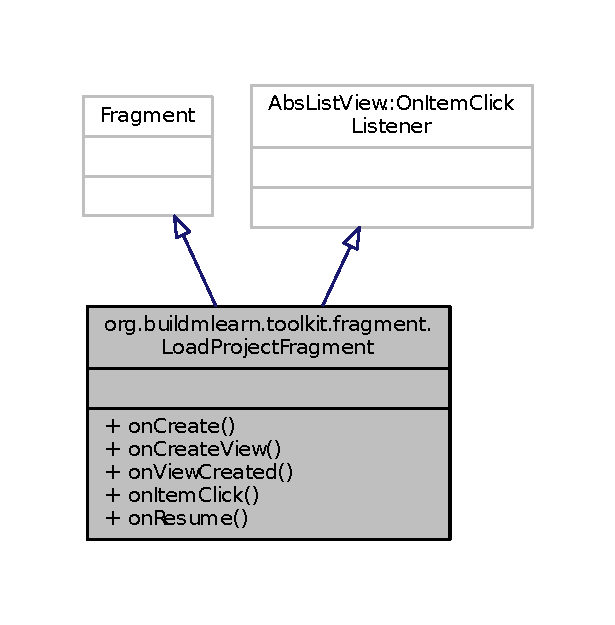
\includegraphics[width=295pt]{d0/dc4/classorg_1_1buildmlearn_1_1toolkit_1_1fragment_1_1LoadProjectFragment__inherit__graph}
\end{center}
\end{figure}


Collaboration diagram for org.\-buildmlearn.\-toolkit.\-fragment.\-Load\-Project\-Fragment\-:
\nopagebreak
\begin{figure}[H]
\begin{center}
\leavevmode
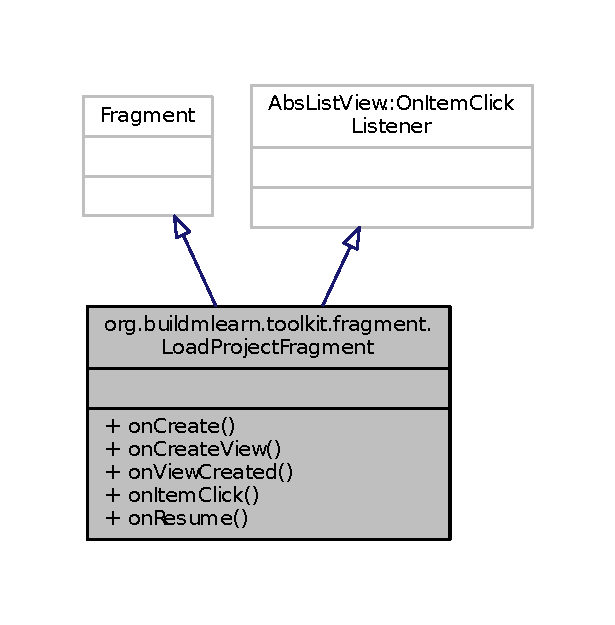
\includegraphics[width=295pt]{dd/d1f/classorg_1_1buildmlearn_1_1toolkit_1_1fragment_1_1LoadProjectFragment__coll__graph}
\end{center}
\end{figure}
\subsection*{Public Member Functions}
\begin{DoxyCompactItemize}
\item 
void \hyperlink{classorg_1_1buildmlearn_1_1toolkit_1_1fragment_1_1LoadProjectFragment_aa3475b8770215affec67dd109da8e9cb}{on\-Create} (Bundle saved\-Instance\-State)
\item 
View \hyperlink{classorg_1_1buildmlearn_1_1toolkit_1_1fragment_1_1LoadProjectFragment_a00df408d1104d5e9da684300c7d1a373}{on\-Create\-View} (Layout\-Inflater inflater, View\-Group container, Bundle saved\-Instance\-State)
\item 
void \hyperlink{classorg_1_1buildmlearn_1_1toolkit_1_1fragment_1_1LoadProjectFragment_a486509578e69cb110ec10c53c6c813c6}{on\-View\-Created} (View view, Bundle saved\-Instance\-State)
\item 
void \hyperlink{classorg_1_1buildmlearn_1_1toolkit_1_1fragment_1_1LoadProjectFragment_ab3fd6e093c178f367cf3403496d30fd5}{on\-Item\-Click} (Adapter\-View$<$?$>$ parent, View view, int position, long id)
\item 
void \hyperlink{classorg_1_1buildmlearn_1_1toolkit_1_1fragment_1_1LoadProjectFragment_af7ebf8d42c3c401e7fcad1fa3850001c}{on\-Resume} ()
\end{DoxyCompactItemize}


\subsection{Detailed Description}
Fragment used for loading existing projects into a list. 

\subsection{Member Function Documentation}
\hypertarget{classorg_1_1buildmlearn_1_1toolkit_1_1fragment_1_1LoadProjectFragment_aa3475b8770215affec67dd109da8e9cb}{\index{org\-::buildmlearn\-::toolkit\-::fragment\-::\-Load\-Project\-Fragment@{org\-::buildmlearn\-::toolkit\-::fragment\-::\-Load\-Project\-Fragment}!on\-Create@{on\-Create}}
\index{on\-Create@{on\-Create}!org::buildmlearn::toolkit::fragment::LoadProjectFragment@{org\-::buildmlearn\-::toolkit\-::fragment\-::\-Load\-Project\-Fragment}}
\subsubsection[{on\-Create}]{\setlength{\rightskip}{0pt plus 5cm}void org.\-buildmlearn.\-toolkit.\-fragment.\-Load\-Project\-Fragment.\-on\-Create (
\begin{DoxyParamCaption}
\item[{Bundle}]{saved\-Instance\-State}
\end{DoxyParamCaption}
)}}\label{classorg_1_1buildmlearn_1_1toolkit_1_1fragment_1_1LoadProjectFragment_aa3475b8770215affec67dd109da8e9cb}

\begin{DoxyCode}
51                                                     \{
52         super.onCreate(savedInstanceState);
53 
54         mToolkit = (ToolkitApplication) getActivity().getApplicationContext();
55         savedProjects = \textcolor{keyword}{new} ArrayList<>();
56 
57         String path = mToolkit.getSavedDir();
58         Log.d(\textcolor{stringliteral}{"Files"}, \textcolor{stringliteral}{"Path: "} + path);
59 
60 
61         File f = \textcolor{keyword}{new} File(path);
62         File file[] = f.listFiles();
63         \textcolor{keywordflow}{if} (file == null) \{
64             \textcolor{keywordflow}{return};
65         \}
66 
67         Log.d(\textcolor{stringliteral}{"Files"}, \textcolor{stringliteral}{"Size: "} + file.length);
68         \textcolor{keywordflow}{for} (\textcolor{keywordtype}{int} i = 0; i < file.length; i++) \{
69 
70             Log.d(TAG, file[i].getAbsolutePath());
71             File fXmlFile = \textcolor{keyword}{new} File(file[i].getAbsolutePath());
72             DocumentBuilderFactory dbFactory = DocumentBuilderFactory.newInstance();
73             DocumentBuilder dBuilder;
74             \textcolor{keywordflow}{try} \{
75                 dBuilder = dbFactory.newDocumentBuilder();
76                 Document doc = dBuilder.parse(fXmlFile);
77                 doc.getDocumentElement().normalize();
78                 Log.d(\textcolor{stringliteral}{"Files"}, \textcolor{stringliteral}{"Root element :"} + doc.getDocumentElement().getAttribute(\textcolor{stringliteral}{"type"}));
79                 savedProjects.add(\textcolor{keyword}{new} SavedProject(fXmlFile, fXmlFile.getName(), fXmlFile.lastModified(), 
      doc.getDocumentElement().getAttribute(\textcolor{stringliteral}{"type"}), fXmlFile.getAbsolutePath()));
80             \} \textcolor{keywordflow}{catch} (ParserConfigurationException e) \{
81                 e.printStackTrace();
82             \} \textcolor{keywordflow}{catch} (SAXException e) \{
83                 e.printStackTrace();
84             \} \textcolor{keywordflow}{catch} (IOException e) \{
85                 e.printStackTrace();
86             \} \textcolor{keywordflow}{catch} (DOMException e) \{
87                 e.printStackTrace();
88             \}
89         \}
90 
91         Collections.sort(savedProjects, \textcolor{keyword}{new} Comparator<SavedProject>() \{
92             \textcolor{keyword}{public} \textcolor{keywordtype}{int} compare(SavedProject f1, SavedProject f2) \{
93                 \textcolor{keywordflow}{return} Long.valueOf(f1.getFile().lastModified()).compareTo(f2.getFile().lastModified());
94             \}
95         \});
96 
97         Collections.reverse(savedProjects);
98     \}
\end{DoxyCode}
\hypertarget{classorg_1_1buildmlearn_1_1toolkit_1_1fragment_1_1LoadProjectFragment_a00df408d1104d5e9da684300c7d1a373}{\index{org\-::buildmlearn\-::toolkit\-::fragment\-::\-Load\-Project\-Fragment@{org\-::buildmlearn\-::toolkit\-::fragment\-::\-Load\-Project\-Fragment}!on\-Create\-View@{on\-Create\-View}}
\index{on\-Create\-View@{on\-Create\-View}!org::buildmlearn::toolkit::fragment::LoadProjectFragment@{org\-::buildmlearn\-::toolkit\-::fragment\-::\-Load\-Project\-Fragment}}
\subsubsection[{on\-Create\-View}]{\setlength{\rightskip}{0pt plus 5cm}View org.\-buildmlearn.\-toolkit.\-fragment.\-Load\-Project\-Fragment.\-on\-Create\-View (
\begin{DoxyParamCaption}
\item[{Layout\-Inflater}]{inflater, }
\item[{View\-Group}]{container, }
\item[{Bundle}]{saved\-Instance\-State}
\end{DoxyParamCaption}
)}}\label{classorg_1_1buildmlearn_1_1toolkit_1_1fragment_1_1LoadProjectFragment_a00df408d1104d5e9da684300c7d1a373}

\begin{DoxyCode}
105                                                         \{
106         View view = inflater.inflate(R.layout.fragment\_loadproject, container, \textcolor{keyword}{false});
107         \textcolor{keywordflow}{return} view;
108     \}
\end{DoxyCode}
\hypertarget{classorg_1_1buildmlearn_1_1toolkit_1_1fragment_1_1LoadProjectFragment_ab3fd6e093c178f367cf3403496d30fd5}{\index{org\-::buildmlearn\-::toolkit\-::fragment\-::\-Load\-Project\-Fragment@{org\-::buildmlearn\-::toolkit\-::fragment\-::\-Load\-Project\-Fragment}!on\-Item\-Click@{on\-Item\-Click}}
\index{on\-Item\-Click@{on\-Item\-Click}!org::buildmlearn::toolkit::fragment::LoadProjectFragment@{org\-::buildmlearn\-::toolkit\-::fragment\-::\-Load\-Project\-Fragment}}
\subsubsection[{on\-Item\-Click}]{\setlength{\rightskip}{0pt plus 5cm}void org.\-buildmlearn.\-toolkit.\-fragment.\-Load\-Project\-Fragment.\-on\-Item\-Click (
\begin{DoxyParamCaption}
\item[{Adapter\-View$<$?$>$}]{parent, }
\item[{View}]{view, }
\item[{int}]{position, }
\item[{long}]{id}
\end{DoxyParamCaption}
)}}\label{classorg_1_1buildmlearn_1_1toolkit_1_1fragment_1_1LoadProjectFragment_ab3fd6e093c178f367cf3403496d30fd5}

\begin{DoxyCode}
125                                                                                      \{
126         SavedProject project = savedProjects.get(position);
127         Template[] templates = Template.values();
128         \textcolor{keywordflow}{for} (\textcolor{keywordtype}{int} i = 0; i < templates.length; i++) \{
129             \textcolor{keywordflow}{if} (project.getType().equals(getString(templates[i].getType()))) \{
130                 Intent intent = \textcolor{keyword}{new} Intent(getActivity(), TemplateEditor.class);
131                 intent.putExtra(\hyperlink{classorg_1_1buildmlearn_1_1toolkit_1_1constant_1_1Constants_a2ee9d59d6a353dc4664ed2e2086dae9d}{Constants.TEMPLATE\_ID}, i);
132                 intent.putExtra(\hyperlink{classorg_1_1buildmlearn_1_1toolkit_1_1constant_1_1Constants_ab2586e8aa144cd7e8b4928186d709ea8}{Constants.PROJECT\_FILE\_PATH}, project.getFullPath
      ());
133                 startActivity(intent);
134                 \textcolor{keywordflow}{return};
135             \}
136         \}
137         Toast.makeText(getActivity(), \textcolor{stringliteral}{"Invalid project file"}, Toast.LENGTH\_SHORT).show();
138     \}
\end{DoxyCode}
\hypertarget{classorg_1_1buildmlearn_1_1toolkit_1_1fragment_1_1LoadProjectFragment_af7ebf8d42c3c401e7fcad1fa3850001c}{\index{org\-::buildmlearn\-::toolkit\-::fragment\-::\-Load\-Project\-Fragment@{org\-::buildmlearn\-::toolkit\-::fragment\-::\-Load\-Project\-Fragment}!on\-Resume@{on\-Resume}}
\index{on\-Resume@{on\-Resume}!org::buildmlearn::toolkit::fragment::LoadProjectFragment@{org\-::buildmlearn\-::toolkit\-::fragment\-::\-Load\-Project\-Fragment}}
\subsubsection[{on\-Resume}]{\setlength{\rightskip}{0pt plus 5cm}void org.\-buildmlearn.\-toolkit.\-fragment.\-Load\-Project\-Fragment.\-on\-Resume (
\begin{DoxyParamCaption}
{}
\end{DoxyParamCaption}
)}}\label{classorg_1_1buildmlearn_1_1toolkit_1_1fragment_1_1LoadProjectFragment_af7ebf8d42c3c401e7fcad1fa3850001c}

\begin{DoxyCode}
158                            \{
159         \textcolor{keywordflow}{if} (mAdapter != null) \{
160 
161             savedProjects.clear();
162 
163             String path = mToolkit.getSavedDir();
164             Log.d(\textcolor{stringliteral}{"Files"}, \textcolor{stringliteral}{"Path: "} + path);
165 
166 
167             File f = \textcolor{keyword}{new} File(path);
168             File file[] = f.listFiles();
169             \textcolor{keywordflow}{if} (file == null) \{
170                 \textcolor{keywordflow}{return};
171             \}
172 
173 
174             Log.d(\textcolor{stringliteral}{"Files"}, \textcolor{stringliteral}{"Size: "} + file.length);
175             \textcolor{keywordflow}{for} (\textcolor{keywordtype}{int} i = 0; i < file.length; i++) \{
176                 File fXmlFile = \textcolor{keyword}{new} File(file[i].getAbsolutePath());
177                 DocumentBuilderFactory dbFactory = DocumentBuilderFactory.newInstance();
178                 DocumentBuilder dBuilder;
179                 \textcolor{keywordflow}{try} \{
180                     dBuilder = dbFactory.newDocumentBuilder();
181                     Document doc = dBuilder.parse(fXmlFile);
182                     doc.getDocumentElement().normalize();
183                     Log.d(\textcolor{stringliteral}{"Files"}, \textcolor{stringliteral}{"Root element :"} + doc.getDocumentElement().getAttribute(\textcolor{stringliteral}{"type"}));
184                     savedProjects.add(\textcolor{keyword}{new} SavedProject(fXmlFile, fXmlFile.getName(), fXmlFile.lastModified(
      ), doc.getDocumentElement().getAttribute(\textcolor{stringliteral}{"type"}), fXmlFile.getAbsolutePath()));
185                 \} \textcolor{keywordflow}{catch} (ParserConfigurationException e) \{
186                     e.printStackTrace();
187                 \} \textcolor{keywordflow}{catch} (SAXException e) \{
188                     e.printStackTrace();
189                 \} \textcolor{keywordflow}{catch} (IOException e) \{
190                     e.printStackTrace();
191                 \} \textcolor{keywordflow}{catch} (DOMException e) \{
192                     e.printStackTrace();
193                 \}
194             \}
195 
196             Collections.sort(savedProjects, \textcolor{keyword}{new} Comparator<SavedProject>() \{
197                 \textcolor{keyword}{public} \textcolor{keywordtype}{int} compare(SavedProject f1, SavedProject f2) \{
198                     \textcolor{keywordflow}{return} Long.valueOf(f1.getFile().lastModified()).compareTo(f2.getFile().lastModified())
      ;
199                 \}
200             \});
201 
202             Collections.reverse(savedProjects);
203             mAdapter.notifyDataSetChanged();
204         \}
205         super.onResume();
206     \}
\end{DoxyCode}
\hypertarget{classorg_1_1buildmlearn_1_1toolkit_1_1fragment_1_1LoadProjectFragment_a486509578e69cb110ec10c53c6c813c6}{\index{org\-::buildmlearn\-::toolkit\-::fragment\-::\-Load\-Project\-Fragment@{org\-::buildmlearn\-::toolkit\-::fragment\-::\-Load\-Project\-Fragment}!on\-View\-Created@{on\-View\-Created}}
\index{on\-View\-Created@{on\-View\-Created}!org::buildmlearn::toolkit::fragment::LoadProjectFragment@{org\-::buildmlearn\-::toolkit\-::fragment\-::\-Load\-Project\-Fragment}}
\subsubsection[{on\-View\-Created}]{\setlength{\rightskip}{0pt plus 5cm}void org.\-buildmlearn.\-toolkit.\-fragment.\-Load\-Project\-Fragment.\-on\-View\-Created (
\begin{DoxyParamCaption}
\item[{View}]{view, }
\item[{Bundle}]{saved\-Instance\-State}
\end{DoxyParamCaption}
)}}\label{classorg_1_1buildmlearn_1_1toolkit_1_1fragment_1_1LoadProjectFragment_a486509578e69cb110ec10c53c6c813c6}

\begin{DoxyCode}
114                                                                     \{
115         mAdapter = \textcolor{keyword}{new} SavedProjectAdapter(getActivity(), savedProjects);
116         mListView = (AbsListView) view.findViewById(android.R.id.list);
117         setAdapter(mAdapter);
118         mListView.setOnItemClickListener(\textcolor{keyword}{this});
119     \}
\end{DoxyCode}


The documentation for this class was generated from the following file\-:\begin{DoxyCompactItemize}
\item 
/\-Buildm\-Learn-\/\-Toolkit-\/\-Android/source-\/code/app/src/main/java/org/buildmlearn/toolkit/fragment/\hyperlink{LoadProjectFragment_8java}{Load\-Project\-Fragment.\-java}\end{DoxyCompactItemize}

\hypertarget{classorg_1_1buildmlearn_1_1toolkit_1_1flashcardtemplate_1_1MainFragment}{\section{org.\-buildmlearn.\-toolkit.\-flashcardtemplate.\-Main\-Fragment Class Reference}
\label{classorg_1_1buildmlearn_1_1toolkit_1_1flashcardtemplate_1_1MainFragment}\index{org.\-buildmlearn.\-toolkit.\-flashcardtemplate.\-Main\-Fragment@{org.\-buildmlearn.\-toolkit.\-flashcardtemplate.\-Main\-Fragment}}
}


Simulator code for Flash Card Template.  




Inheritance diagram for org.\-buildmlearn.\-toolkit.\-flashcardtemplate.\-Main\-Fragment\-:
\nopagebreak
\begin{figure}[H]
\begin{center}
\leavevmode
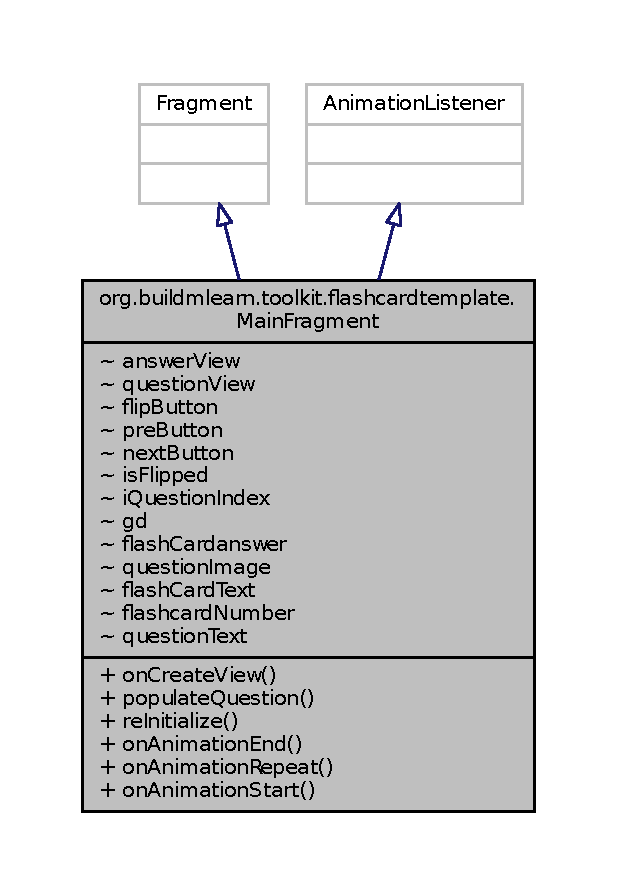
\includegraphics[width=296pt]{d9/dfe/classorg_1_1buildmlearn_1_1toolkit_1_1flashcardtemplate_1_1MainFragment__inherit__graph}
\end{center}
\end{figure}


Collaboration diagram for org.\-buildmlearn.\-toolkit.\-flashcardtemplate.\-Main\-Fragment\-:
\nopagebreak
\begin{figure}[H]
\begin{center}
\leavevmode
\includegraphics[width=350pt]{d4/daf/classorg_1_1buildmlearn_1_1toolkit_1_1flashcardtemplate_1_1MainFragment__coll__graph}
\end{center}
\end{figure}
\subsection*{Public Member Functions}
\begin{DoxyCompactItemize}
\item 
View \hyperlink{classorg_1_1buildmlearn_1_1toolkit_1_1flashcardtemplate_1_1MainFragment_a4a45ac52c1f059e73b6428c8e6497ce2}{on\-Create\-View} (Layout\-Inflater inflater, View\-Group container, Bundle saved\-Instance\-State)
\item 
void \hyperlink{classorg_1_1buildmlearn_1_1toolkit_1_1flashcardtemplate_1_1MainFragment_a4cbd053b83f6e1d0296a7d60639dfd8d}{populate\-Question} (int index)
\item 
void \hyperlink{classorg_1_1buildmlearn_1_1toolkit_1_1flashcardtemplate_1_1MainFragment_ae9e2c735c811355694eb801713f4d900}{re\-Initialize} ()
\item 
void \hyperlink{classorg_1_1buildmlearn_1_1toolkit_1_1flashcardtemplate_1_1MainFragment_a3bf2edf287b796f71a8e2501b7e0d096}{on\-Animation\-End} (Animation animation)
\item 
void \hyperlink{classorg_1_1buildmlearn_1_1toolkit_1_1flashcardtemplate_1_1MainFragment_ad63767eb4d6d68f4e85c64ccc719da37}{on\-Animation\-Repeat} (Animation animation)
\item 
void \hyperlink{classorg_1_1buildmlearn_1_1toolkit_1_1flashcardtemplate_1_1MainFragment_a4fe7d6269f507e5485fe13d036b4f152}{on\-Animation\-Start} (Animation animation)
\end{DoxyCompactItemize}


\subsection{Detailed Description}
Simulator code for Flash Card Template. 

\subsection{Member Function Documentation}
\hypertarget{classorg_1_1buildmlearn_1_1toolkit_1_1flashcardtemplate_1_1MainFragment_a3bf2edf287b796f71a8e2501b7e0d096}{\index{org\-::buildmlearn\-::toolkit\-::flashcardtemplate\-::\-Main\-Fragment@{org\-::buildmlearn\-::toolkit\-::flashcardtemplate\-::\-Main\-Fragment}!on\-Animation\-End@{on\-Animation\-End}}
\index{on\-Animation\-End@{on\-Animation\-End}!org::buildmlearn::toolkit::flashcardtemplate::MainFragment@{org\-::buildmlearn\-::toolkit\-::flashcardtemplate\-::\-Main\-Fragment}}
\subsubsection[{on\-Animation\-End}]{\setlength{\rightskip}{0pt plus 5cm}void org.\-buildmlearn.\-toolkit.\-flashcardtemplate.\-Main\-Fragment.\-on\-Animation\-End (
\begin{DoxyParamCaption}
\item[{Animation}]{animation}
\end{DoxyParamCaption}
)}}\label{classorg_1_1buildmlearn_1_1toolkit_1_1flashcardtemplate_1_1MainFragment_a3bf2edf287b796f71a8e2501b7e0d096}

\begin{DoxyCode}
166                                                     \{
167         \textcolor{keywordflow}{if} (animation == animation1) \{
168 
169             TextView answerText = (TextView) view.findViewById(R.id.answerText);
170 
171             \textcolor{keywordflow}{if} (!isFlipped) \{
172 
173                 answerView.setVisibility(View.VISIBLE);
174                 questionView.setVisibility(View.GONE);
175                 isFlipped = \textcolor{keyword}{true};
176                 answerText.setText(flashCardanswer);
177                 currentView = answerView;
178             \} \textcolor{keywordflow}{else} \{
179 
180                 isFlipped = \textcolor{keyword}{false};
181                 answerText.setText(\textcolor{stringliteral}{""});
182                 questionView.setVisibility(View.VISIBLE);
183                 answerView.setVisibility(View.GONE);
184                 currentView = questionView;
185             \}
186             currentView.clearAnimation();
187             currentView.setAnimation(animation2);
188             currentView.startAnimation(animation2);
189 
190         \}
191 
192     \}
\end{DoxyCode}
\hypertarget{classorg_1_1buildmlearn_1_1toolkit_1_1flashcardtemplate_1_1MainFragment_ad63767eb4d6d68f4e85c64ccc719da37}{\index{org\-::buildmlearn\-::toolkit\-::flashcardtemplate\-::\-Main\-Fragment@{org\-::buildmlearn\-::toolkit\-::flashcardtemplate\-::\-Main\-Fragment}!on\-Animation\-Repeat@{on\-Animation\-Repeat}}
\index{on\-Animation\-Repeat@{on\-Animation\-Repeat}!org::buildmlearn::toolkit::flashcardtemplate::MainFragment@{org\-::buildmlearn\-::toolkit\-::flashcardtemplate\-::\-Main\-Fragment}}
\subsubsection[{on\-Animation\-Repeat}]{\setlength{\rightskip}{0pt plus 5cm}void org.\-buildmlearn.\-toolkit.\-flashcardtemplate.\-Main\-Fragment.\-on\-Animation\-Repeat (
\begin{DoxyParamCaption}
\item[{Animation}]{animation}
\end{DoxyParamCaption}
)}}\label{classorg_1_1buildmlearn_1_1toolkit_1_1flashcardtemplate_1_1MainFragment_ad63767eb4d6d68f4e85c64ccc719da37}

\begin{DoxyCode}
195                                                        \{
196         \textcolor{comment}{// TODO Auto-generated method stub}
197 
198     \}
\end{DoxyCode}
\hypertarget{classorg_1_1buildmlearn_1_1toolkit_1_1flashcardtemplate_1_1MainFragment_a4fe7d6269f507e5485fe13d036b4f152}{\index{org\-::buildmlearn\-::toolkit\-::flashcardtemplate\-::\-Main\-Fragment@{org\-::buildmlearn\-::toolkit\-::flashcardtemplate\-::\-Main\-Fragment}!on\-Animation\-Start@{on\-Animation\-Start}}
\index{on\-Animation\-Start@{on\-Animation\-Start}!org::buildmlearn::toolkit::flashcardtemplate::MainFragment@{org\-::buildmlearn\-::toolkit\-::flashcardtemplate\-::\-Main\-Fragment}}
\subsubsection[{on\-Animation\-Start}]{\setlength{\rightskip}{0pt plus 5cm}void org.\-buildmlearn.\-toolkit.\-flashcardtemplate.\-Main\-Fragment.\-on\-Animation\-Start (
\begin{DoxyParamCaption}
\item[{Animation}]{animation}
\end{DoxyParamCaption}
)}}\label{classorg_1_1buildmlearn_1_1toolkit_1_1flashcardtemplate_1_1MainFragment_a4fe7d6269f507e5485fe13d036b4f152}

\begin{DoxyCode}
201                                                       \{
202         \textcolor{comment}{// TODO Auto-generated method stub}
203 
204     \}
\end{DoxyCode}
\hypertarget{classorg_1_1buildmlearn_1_1toolkit_1_1flashcardtemplate_1_1MainFragment_a4a45ac52c1f059e73b6428c8e6497ce2}{\index{org\-::buildmlearn\-::toolkit\-::flashcardtemplate\-::\-Main\-Fragment@{org\-::buildmlearn\-::toolkit\-::flashcardtemplate\-::\-Main\-Fragment}!on\-Create\-View@{on\-Create\-View}}
\index{on\-Create\-View@{on\-Create\-View}!org::buildmlearn::toolkit::flashcardtemplate::MainFragment@{org\-::buildmlearn\-::toolkit\-::flashcardtemplate\-::\-Main\-Fragment}}
\subsubsection[{on\-Create\-View}]{\setlength{\rightskip}{0pt plus 5cm}View org.\-buildmlearn.\-toolkit.\-flashcardtemplate.\-Main\-Fragment.\-on\-Create\-View (
\begin{DoxyParamCaption}
\item[{Layout\-Inflater}]{inflater, }
\item[{View\-Group}]{container, }
\item[{Bundle}]{saved\-Instance\-State}
\end{DoxyParamCaption}
)}}\label{classorg_1_1buildmlearn_1_1toolkit_1_1flashcardtemplate_1_1MainFragment_a4a45ac52c1f059e73b6428c8e6497ce2}

\begin{DoxyCode}
47                                                                                                       \{
48 
49         view = inflater.inflate(R.layout.flash\_simu\_main, container, \textcolor{keyword}{false});
50 
51         animation1 = AnimationUtils.loadAnimation(getActivity(), R.anim.to\_middle);
52         animation1.setAnimationListener(\textcolor{keyword}{this});
53         animation2 = AnimationUtils.loadAnimation(getActivity(), R.anim.from\_middle);
54         animation2.setAnimationListener(\textcolor{keyword}{this});
55 
56         questionView = view.findViewById(R.id.questionInMain);
57         answerView = view.findViewById(R.id.answerInMain);
58 
59         questionView.setVisibility(View.VISIBLE);
60         answerView.setVisibility(View.GONE);
61         iQuestionIndex = 0;
62 
63         questionImage = (ImageView) view.findViewById(R.id.questionImage);
64         flashCardText = (TextView) view.findViewById(R.id.flashCardText);
65         questionText = (TextView) view.findViewById(R.id.questionhint);
66         flashcardNumber = (TextView) view.findViewById(R.id.flashCardNumber);
67 
68         flipButton = (Button) view.findViewById(R.id.flip\_button);
69         preButton = (Button) view.findViewById(R.id.pre\_button);
70         nextButton = (Button) view.findViewById(R.id.next\_button);
71 
72         \hyperlink{classorg_1_1buildmlearn_1_1toolkit_1_1flashcardtemplate_1_1MainFragment_a4cbd053b83f6e1d0296a7d60639dfd8d}{populateQuestion}(iQuestionIndex);
73         currentView = questionView;
74 
75         flipButton.setOnClickListener(\textcolor{keyword}{new} OnClickListener() \{
76 
77             @Override
78             \textcolor{keyword}{public} \textcolor{keywordtype}{void} onClick(View v) \{
79 
80                 currentView.clearAnimation();
81                 currentView.setAnimation(animation1);
82                 currentView.startAnimation(animation1);
83 
84             \}
85         \});
86 
87         preButton.setOnClickListener(\textcolor{keyword}{new} OnClickListener() \{
88 
89             @Override
90             \textcolor{keyword}{public} \textcolor{keywordtype}{void} onClick(View v) \{
91                 \textcolor{keywordflow}{if} (iQuestionIndex != 0) \{
92                     isFlipped = \textcolor{keyword}{false};
93 
94                     iQuestionIndex--;
95                     questionView.setVisibility(View.VISIBLE);
96                     answerView.setVisibility(View.GONE);
97                     currentView = questionView;
98 
99                     \hyperlink{classorg_1_1buildmlearn_1_1toolkit_1_1flashcardtemplate_1_1MainFragment_a4cbd053b83f6e1d0296a7d60639dfd8d}{populateQuestion}(iQuestionIndex);
100                 \}
101 
102             \}
103         \});
104 
105         nextButton.setOnClickListener(\textcolor{keyword}{new} OnClickListener() \{
106 
107             @Override
108             \textcolor{keyword}{public} \textcolor{keywordtype}{void} onClick(View v) \{
109 
110                 \textcolor{keywordflow}{if} (iQuestionIndex < gd.model.size() - 1) \{
111                     isFlipped = \textcolor{keyword}{false};
112                     iQuestionIndex++;
113                     questionView.setVisibility(View.VISIBLE);
114                     answerView.setVisibility(View.GONE);
115                     currentView = questionView;
116                     \hyperlink{classorg_1_1buildmlearn_1_1toolkit_1_1flashcardtemplate_1_1MainFragment_a4cbd053b83f6e1d0296a7d60639dfd8d}{populateQuestion}(iQuestionIndex);
117 
118                 \} \textcolor{keywordflow}{else} \{
119 
120                     getActivity().getFragmentManager().beginTransaction().replace(R.id.container, \textcolor{keyword}{new} 
      ScoreFragment()).addToBackStack(null).commit();
121 
122                     \hyperlink{classorg_1_1buildmlearn_1_1toolkit_1_1flashcardtemplate_1_1MainFragment_ae9e2c735c811355694eb801713f4d900}{reInitialize}();
123                 \}
124 
125             \}
126         \});
127         \textcolor{keywordflow}{return} view;
128     \}
\end{DoxyCode}
\hypertarget{classorg_1_1buildmlearn_1_1toolkit_1_1flashcardtemplate_1_1MainFragment_a4cbd053b83f6e1d0296a7d60639dfd8d}{\index{org\-::buildmlearn\-::toolkit\-::flashcardtemplate\-::\-Main\-Fragment@{org\-::buildmlearn\-::toolkit\-::flashcardtemplate\-::\-Main\-Fragment}!populate\-Question@{populate\-Question}}
\index{populate\-Question@{populate\-Question}!org::buildmlearn::toolkit::flashcardtemplate::MainFragment@{org\-::buildmlearn\-::toolkit\-::flashcardtemplate\-::\-Main\-Fragment}}
\subsubsection[{populate\-Question}]{\setlength{\rightskip}{0pt plus 5cm}void org.\-buildmlearn.\-toolkit.\-flashcardtemplate.\-Main\-Fragment.\-populate\-Question (
\begin{DoxyParamCaption}
\item[{int}]{index}
\end{DoxyParamCaption}
)}}\label{classorg_1_1buildmlearn_1_1toolkit_1_1flashcardtemplate_1_1MainFragment_a4cbd053b83f6e1d0296a7d60639dfd8d}

\begin{DoxyCode}
131                                             \{
132         \textcolor{keywordflow}{if} (index == 0) \{
133             preButton.setEnabled(\textcolor{keyword}{false});
134 
135         \} \textcolor{keywordflow}{else}
136             preButton.setEnabled(\textcolor{keyword}{true});
137 
138         \textcolor{keywordtype}{int} cardNum = index + 1;
139         flashcardNumber.setText(\textcolor{stringliteral}{"Card #"} + cardNum + \textcolor{stringliteral}{" of "} + gd.totalCards);
140         FlashModel mFlash = gd.model.get(index);
141         TextView answerText = (TextView) view.findViewById(R.id.answerText);
142         \textcolor{keywordflow}{if} (mFlash.getQuestion() != null)
143             questionText.setText(mFlash.getQuestion());
144         \textcolor{keywordflow}{if} (mFlash.getAnswer() != null) \{
145             flashCardanswer = mFlash.getAnswer();
146             answerText.setText(mFlash.getAnswer());
147         \}
148         \textcolor{keywordflow}{if} (mFlash.getBase64() != null) \{
149             byte[] decodedString = Base64.decode(mFlash.getBase64(),
150                     Base64.DEFAULT);
151             Bitmap decodedByte = BitmapFactory.decodeByteArray(decodedString,
152                     0, decodedString.length);
153             questionImage.setImageBitmap(decodedByte);
154         \} \textcolor{keywordflow}{else} \{
155             questionText.setGravity(Gravity.CENTER\_VERTICAL);
156         \}
157 
158     \}
\end{DoxyCode}
\hypertarget{classorg_1_1buildmlearn_1_1toolkit_1_1flashcardtemplate_1_1MainFragment_ae9e2c735c811355694eb801713f4d900}{\index{org\-::buildmlearn\-::toolkit\-::flashcardtemplate\-::\-Main\-Fragment@{org\-::buildmlearn\-::toolkit\-::flashcardtemplate\-::\-Main\-Fragment}!re\-Initialize@{re\-Initialize}}
\index{re\-Initialize@{re\-Initialize}!org::buildmlearn::toolkit::flashcardtemplate::MainFragment@{org\-::buildmlearn\-::toolkit\-::flashcardtemplate\-::\-Main\-Fragment}}
\subsubsection[{re\-Initialize}]{\setlength{\rightskip}{0pt plus 5cm}void org.\-buildmlearn.\-toolkit.\-flashcardtemplate.\-Main\-Fragment.\-re\-Initialize (
\begin{DoxyParamCaption}
{}
\end{DoxyParamCaption}
)}}\label{classorg_1_1buildmlearn_1_1toolkit_1_1flashcardtemplate_1_1MainFragment_ae9e2c735c811355694eb801713f4d900}

\begin{DoxyCode}
160                                \{
161         iQuestionIndex = 0;
162         gd.model.clear();
163     \}
\end{DoxyCode}


The documentation for this class was generated from the following file\-:\begin{DoxyCompactItemize}
\item 
/\-Buildm\-Learn-\/\-Toolkit-\/\-Android/source-\/code/app/src/main/java/org/buildmlearn/toolkit/flashcardtemplate/\hyperlink{MainFragment_8java}{Main\-Fragment.\-java}\end{DoxyCompactItemize}

\hypertarget{interfaceorg_1_1buildmlearn_1_1toolkit_1_1fragment_1_1NavigationDrawerFragment_1_1NavigationDrawerCallbacks}{\section{org.\-buildmlearn.\-toolkit.\-fragment.\-Navigation\-Drawer\-Fragment.\-Navigation\-Drawer\-Callbacks Interface Reference}
\label{interfaceorg_1_1buildmlearn_1_1toolkit_1_1fragment_1_1NavigationDrawerFragment_1_1NavigationDrawerCallbacks}\index{org.\-buildmlearn.\-toolkit.\-fragment.\-Navigation\-Drawer\-Fragment.\-Navigation\-Drawer\-Callbacks@{org.\-buildmlearn.\-toolkit.\-fragment.\-Navigation\-Drawer\-Fragment.\-Navigation\-Drawer\-Callbacks}}
}


Inheritance diagram for org.\-buildmlearn.\-toolkit.\-fragment.\-Navigation\-Drawer\-Fragment.\-Navigation\-Drawer\-Callbacks\-:
\nopagebreak
\begin{figure}[H]
\begin{center}
\leavevmode
\includegraphics[width=280pt]{d6/d14/interfaceorg_1_1buildmlearn_1_1toolkit_1_1fragment_1_1NavigationDrawerFragment_1_1NavigationDrawerCallbacks__inherit__graph}
\end{center}
\end{figure}


Collaboration diagram for org.\-buildmlearn.\-toolkit.\-fragment.\-Navigation\-Drawer\-Fragment.\-Navigation\-Drawer\-Callbacks\-:
\nopagebreak
\begin{figure}[H]
\begin{center}
\leavevmode
\includegraphics[width=280pt]{d2/d33/interfaceorg_1_1buildmlearn_1_1toolkit_1_1fragment_1_1NavigationDrawerFragment_1_1NavigationDrawerCallbacks__coll__graph}
\end{center}
\end{figure}
\subsection*{Public Member Functions}
\begin{DoxyCompactItemize}
\item 
void \hyperlink{interfaceorg_1_1buildmlearn_1_1toolkit_1_1fragment_1_1NavigationDrawerFragment_1_1NavigationDrawerCallbacks_a6068a4dec53d00ec47c222f995064e6c}{on\-Navigation\-Drawer\-Item\-Selected} (int position)
\end{DoxyCompactItemize}


\subsection{Detailed Description}
Callbacks interface that all activities using this fragment must implement. 

\subsection{Member Function Documentation}
\hypertarget{interfaceorg_1_1buildmlearn_1_1toolkit_1_1fragment_1_1NavigationDrawerFragment_1_1NavigationDrawerCallbacks_a6068a4dec53d00ec47c222f995064e6c}{\index{org\-::buildmlearn\-::toolkit\-::fragment\-::\-Navigation\-Drawer\-Fragment\-::\-Navigation\-Drawer\-Callbacks@{org\-::buildmlearn\-::toolkit\-::fragment\-::\-Navigation\-Drawer\-Fragment\-::\-Navigation\-Drawer\-Callbacks}!on\-Navigation\-Drawer\-Item\-Selected@{on\-Navigation\-Drawer\-Item\-Selected}}
\index{on\-Navigation\-Drawer\-Item\-Selected@{on\-Navigation\-Drawer\-Item\-Selected}!org::buildmlearn::toolkit::fragment::NavigationDrawerFragment::NavigationDrawerCallbacks@{org\-::buildmlearn\-::toolkit\-::fragment\-::\-Navigation\-Drawer\-Fragment\-::\-Navigation\-Drawer\-Callbacks}}
\subsubsection[{on\-Navigation\-Drawer\-Item\-Selected}]{\setlength{\rightskip}{0pt plus 5cm}void org.\-buildmlearn.\-toolkit.\-fragment.\-Navigation\-Drawer\-Fragment.\-Navigation\-Drawer\-Callbacks.\-on\-Navigation\-Drawer\-Item\-Selected (
\begin{DoxyParamCaption}
\item[{int}]{position}
\end{DoxyParamCaption}
)}}\label{interfaceorg_1_1buildmlearn_1_1toolkit_1_1fragment_1_1NavigationDrawerFragment_1_1NavigationDrawerCallbacks_a6068a4dec53d00ec47c222f995064e6c}
Called when an item in the navigation drawer is selected. 

Implemented in \hyperlink{classorg_1_1buildmlearn_1_1toolkit_1_1activity_1_1HomeActivity_af75c80f626f8c3a7141c046108ff229f}{org.\-buildmlearn.\-toolkit.\-activity.\-Home\-Activity}.



The documentation for this interface was generated from the following file\-:\begin{DoxyCompactItemize}
\item 
/\-Buildm\-Learn-\/\-Toolkit-\/\-Android/source-\/code/app/src/main/java/org/buildmlearn/toolkit/fragment/\hyperlink{NavigationDrawerFragment_8java}{Navigation\-Drawer\-Fragment.\-java}\end{DoxyCompactItemize}

\hypertarget{classorg_1_1buildmlearn_1_1toolkit_1_1fragment_1_1NavigationDrawerFragment}{\section{org.\-buildmlearn.\-toolkit.\-fragment.\-Navigation\-Drawer\-Fragment Class Reference}
\label{classorg_1_1buildmlearn_1_1toolkit_1_1fragment_1_1NavigationDrawerFragment}\index{org.\-buildmlearn.\-toolkit.\-fragment.\-Navigation\-Drawer\-Fragment@{org.\-buildmlearn.\-toolkit.\-fragment.\-Navigation\-Drawer\-Fragment}}
}


Inheritance diagram for org.\-buildmlearn.\-toolkit.\-fragment.\-Navigation\-Drawer\-Fragment\-:
\nopagebreak
\begin{figure}[H]
\begin{center}
\leavevmode
\includegraphics[width=254pt]{d7/ddf/classorg_1_1buildmlearn_1_1toolkit_1_1fragment_1_1NavigationDrawerFragment__inherit__graph}
\end{center}
\end{figure}


Collaboration diagram for org.\-buildmlearn.\-toolkit.\-fragment.\-Navigation\-Drawer\-Fragment\-:
\nopagebreak
\begin{figure}[H]
\begin{center}
\leavevmode
\includegraphics[width=254pt]{d3/d5d/classorg_1_1buildmlearn_1_1toolkit_1_1fragment_1_1NavigationDrawerFragment__coll__graph}
\end{center}
\end{figure}
\subsection*{Classes}
\begin{DoxyCompactItemize}
\item 
interface \hyperlink{interfaceorg_1_1buildmlearn_1_1toolkit_1_1fragment_1_1NavigationDrawerFragment_1_1NavigationDrawerCallbacks}{Navigation\-Drawer\-Callbacks}
\end{DoxyCompactItemize}
\subsection*{Public Member Functions}
\begin{DoxyCompactItemize}
\item 
\hyperlink{classorg_1_1buildmlearn_1_1toolkit_1_1fragment_1_1NavigationDrawerFragment_a5f3f1b07fbb49a4d21f98008e702e8d4}{Navigation\-Drawer\-Fragment} ()
\item 
void \hyperlink{classorg_1_1buildmlearn_1_1toolkit_1_1fragment_1_1NavigationDrawerFragment_a7a9c297215fb754ea5bd3745233cec21}{on\-Create} (Bundle saved\-Instance\-State)
\item 
void \hyperlink{classorg_1_1buildmlearn_1_1toolkit_1_1fragment_1_1NavigationDrawerFragment_a734263415ae5341ea1cb5b4b2a469581}{on\-Activity\-Created} (Bundle saved\-Instance\-State)
\item 
View \hyperlink{classorg_1_1buildmlearn_1_1toolkit_1_1fragment_1_1NavigationDrawerFragment_a960b71d9ccecc621b4a5506f38a105cf}{on\-Create\-View} (Layout\-Inflater inflater, View\-Group container, Bundle saved\-Instance\-State)
\item 
boolean \hyperlink{classorg_1_1buildmlearn_1_1toolkit_1_1fragment_1_1NavigationDrawerFragment_a85975c4bf9994479fb882843b31988b5}{is\-Drawer\-Open} ()
\item 
void \hyperlink{classorg_1_1buildmlearn_1_1toolkit_1_1fragment_1_1NavigationDrawerFragment_a6ec051ce4329da7861cc19a0e01ed01b}{set\-Up} (int fragment\-Id, Drawer\-Layout drawer\-Layout)
\item 
void \hyperlink{classorg_1_1buildmlearn_1_1toolkit_1_1fragment_1_1NavigationDrawerFragment_ab5f8207c0919a7add76e3de6ea407ae0}{on\-Attach} (Activity activity)
\item 
void \hyperlink{classorg_1_1buildmlearn_1_1toolkit_1_1fragment_1_1NavigationDrawerFragment_af5ec3253d086d2733aea3a595061c389}{on\-Detach} ()
\item 
void \hyperlink{classorg_1_1buildmlearn_1_1toolkit_1_1fragment_1_1NavigationDrawerFragment_a3ecc348d09897125baff9673c4145a55}{on\-Save\-Instance\-State} (Bundle out\-State)
\item 
void \hyperlink{classorg_1_1buildmlearn_1_1toolkit_1_1fragment_1_1NavigationDrawerFragment_aa216d0cfc2c54c3cd6c9f91cb005cea1}{on\-Configuration\-Changed} (Configuration new\-Config)
\item 
void \hyperlink{classorg_1_1buildmlearn_1_1toolkit_1_1fragment_1_1NavigationDrawerFragment_a23412cd6598c10cee64ff60848cc6771}{on\-Create\-Options\-Menu} (Menu menu, Menu\-Inflater inflater)
\item 
boolean \hyperlink{classorg_1_1buildmlearn_1_1toolkit_1_1fragment_1_1NavigationDrawerFragment_a68eb844e52918f108a9145c9fd9e1bee}{on\-Options\-Item\-Selected} (Menu\-Item item)
\end{DoxyCompactItemize}
\subsection*{Protected Member Functions}
\begin{DoxyCompactItemize}
\item 
void \hyperlink{classorg_1_1buildmlearn_1_1toolkit_1_1fragment_1_1NavigationDrawerFragment_a082efc992fd2f9af81579c038f1c1bd0}{show\-Global\-Context\-Action\-Bar} ()
\item 
Action\-Bar \hyperlink{classorg_1_1buildmlearn_1_1toolkit_1_1fragment_1_1NavigationDrawerFragment_a84ffac4d244a528b278d27732387b551}{get\-Action\-Bar} ()
\end{DoxyCompactItemize}


\subsection{Detailed Description}
Fragment used for managing interactions for and presentation of a navigation drawer. See the \href{https://developer.android.com/design/patterns/navigation-drawer.html#Interaction}{\tt design guidelines} for a complete explanation of the behaviors implemented here. 

\subsection{Constructor \& Destructor Documentation}
\hypertarget{classorg_1_1buildmlearn_1_1toolkit_1_1fragment_1_1NavigationDrawerFragment_a5f3f1b07fbb49a4d21f98008e702e8d4}{\index{org\-::buildmlearn\-::toolkit\-::fragment\-::\-Navigation\-Drawer\-Fragment@{org\-::buildmlearn\-::toolkit\-::fragment\-::\-Navigation\-Drawer\-Fragment}!Navigation\-Drawer\-Fragment@{Navigation\-Drawer\-Fragment}}
\index{Navigation\-Drawer\-Fragment@{Navigation\-Drawer\-Fragment}!org::buildmlearn::toolkit::fragment::NavigationDrawerFragment@{org\-::buildmlearn\-::toolkit\-::fragment\-::\-Navigation\-Drawer\-Fragment}}
\subsubsection[{Navigation\-Drawer\-Fragment}]{\setlength{\rightskip}{0pt plus 5cm}org.\-buildmlearn.\-toolkit.\-fragment.\-Navigation\-Drawer\-Fragment.\-Navigation\-Drawer\-Fragment (
\begin{DoxyParamCaption}
{}
\end{DoxyParamCaption}
)}}\label{classorg_1_1buildmlearn_1_1toolkit_1_1fragment_1_1NavigationDrawerFragment_a5f3f1b07fbb49a4d21f98008e702e8d4}

\begin{DoxyCode}
67                                       \{
68     \}
\end{DoxyCode}


\subsection{Member Function Documentation}
\hypertarget{classorg_1_1buildmlearn_1_1toolkit_1_1fragment_1_1NavigationDrawerFragment_a84ffac4d244a528b278d27732387b551}{\index{org\-::buildmlearn\-::toolkit\-::fragment\-::\-Navigation\-Drawer\-Fragment@{org\-::buildmlearn\-::toolkit\-::fragment\-::\-Navigation\-Drawer\-Fragment}!get\-Action\-Bar@{get\-Action\-Bar}}
\index{get\-Action\-Bar@{get\-Action\-Bar}!org::buildmlearn::toolkit::fragment::NavigationDrawerFragment@{org\-::buildmlearn\-::toolkit\-::fragment\-::\-Navigation\-Drawer\-Fragment}}
\subsubsection[{get\-Action\-Bar}]{\setlength{\rightskip}{0pt plus 5cm}Action\-Bar org.\-buildmlearn.\-toolkit.\-fragment.\-Navigation\-Drawer\-Fragment.\-get\-Action\-Bar (
\begin{DoxyParamCaption}
{}
\end{DoxyParamCaption}
)\hspace{0.3cm}{\ttfamily [protected]}}}\label{classorg_1_1buildmlearn_1_1toolkit_1_1fragment_1_1NavigationDrawerFragment_a84ffac4d244a528b278d27732387b551}

\begin{DoxyCode}
321                                        \{
322         \textcolor{keywordflow}{return} ((AppCompatActivity) getActivity()).getSupportActionBar();
323     \}
\end{DoxyCode}
\hypertarget{classorg_1_1buildmlearn_1_1toolkit_1_1fragment_1_1NavigationDrawerFragment_a85975c4bf9994479fb882843b31988b5}{\index{org\-::buildmlearn\-::toolkit\-::fragment\-::\-Navigation\-Drawer\-Fragment@{org\-::buildmlearn\-::toolkit\-::fragment\-::\-Navigation\-Drawer\-Fragment}!is\-Drawer\-Open@{is\-Drawer\-Open}}
\index{is\-Drawer\-Open@{is\-Drawer\-Open}!org::buildmlearn::toolkit::fragment::NavigationDrawerFragment@{org\-::buildmlearn\-::toolkit\-::fragment\-::\-Navigation\-Drawer\-Fragment}}
\subsubsection[{is\-Drawer\-Open}]{\setlength{\rightskip}{0pt plus 5cm}boolean org.\-buildmlearn.\-toolkit.\-fragment.\-Navigation\-Drawer\-Fragment.\-is\-Drawer\-Open (
\begin{DoxyParamCaption}
{}
\end{DoxyParamCaption}
)}}\label{classorg_1_1buildmlearn_1_1toolkit_1_1fragment_1_1NavigationDrawerFragment_a85975c4bf9994479fb882843b31988b5}

\begin{DoxyCode}
138                                   \{
139         \textcolor{keywordflow}{return} mDrawerLayout != null && mDrawerLayout.isDrawerOpen(mFragmentContainerView);
140     \}
\end{DoxyCode}
\hypertarget{classorg_1_1buildmlearn_1_1toolkit_1_1fragment_1_1NavigationDrawerFragment_a734263415ae5341ea1cb5b4b2a469581}{\index{org\-::buildmlearn\-::toolkit\-::fragment\-::\-Navigation\-Drawer\-Fragment@{org\-::buildmlearn\-::toolkit\-::fragment\-::\-Navigation\-Drawer\-Fragment}!on\-Activity\-Created@{on\-Activity\-Created}}
\index{on\-Activity\-Created@{on\-Activity\-Created}!org::buildmlearn::toolkit::fragment::NavigationDrawerFragment@{org\-::buildmlearn\-::toolkit\-::fragment\-::\-Navigation\-Drawer\-Fragment}}
\subsubsection[{on\-Activity\-Created}]{\setlength{\rightskip}{0pt plus 5cm}void org.\-buildmlearn.\-toolkit.\-fragment.\-Navigation\-Drawer\-Fragment.\-on\-Activity\-Created (
\begin{DoxyParamCaption}
\item[{Bundle}]{saved\-Instance\-State}
\end{DoxyParamCaption}
)}}\label{classorg_1_1buildmlearn_1_1toolkit_1_1fragment_1_1NavigationDrawerFragment_a734263415ae5341ea1cb5b4b2a469581}

\begin{DoxyCode}
96                                                              \{
97         super.onActivityCreated(savedInstanceState);
98         \textcolor{comment}{// Indicate that this fragment would like to influence the set of actions in the action bar.}
99         setHasOptionsMenu(\textcolor{keyword}{true});
100     \}
\end{DoxyCode}
\hypertarget{classorg_1_1buildmlearn_1_1toolkit_1_1fragment_1_1NavigationDrawerFragment_ab5f8207c0919a7add76e3de6ea407ae0}{\index{org\-::buildmlearn\-::toolkit\-::fragment\-::\-Navigation\-Drawer\-Fragment@{org\-::buildmlearn\-::toolkit\-::fragment\-::\-Navigation\-Drawer\-Fragment}!on\-Attach@{on\-Attach}}
\index{on\-Attach@{on\-Attach}!org::buildmlearn::toolkit::fragment::NavigationDrawerFragment@{org\-::buildmlearn\-::toolkit\-::fragment\-::\-Navigation\-Drawer\-Fragment}}
\subsubsection[{on\-Attach}]{\setlength{\rightskip}{0pt plus 5cm}void org.\-buildmlearn.\-toolkit.\-fragment.\-Navigation\-Drawer\-Fragment.\-on\-Attach (
\begin{DoxyParamCaption}
\item[{Activity}]{activity}
\end{DoxyParamCaption}
)}}\label{classorg_1_1buildmlearn_1_1toolkit_1_1fragment_1_1NavigationDrawerFragment_ab5f8207c0919a7add76e3de6ea407ae0}

\begin{DoxyCode}
247                                             \{
248         super.onAttach(activity);
249         \textcolor{keywordflow}{try} \{
250             mCallbacks = (NavigationDrawerCallbacks) activity;
251         \} \textcolor{keywordflow}{catch} (ClassCastException e) \{
252             \textcolor{keywordflow}{throw} \textcolor{keyword}{new} ClassCastException(\textcolor{stringliteral}{"Activity must implement NavigationDrawerCallbacks."});
253         \}
254     \}
\end{DoxyCode}
\hypertarget{classorg_1_1buildmlearn_1_1toolkit_1_1fragment_1_1NavigationDrawerFragment_aa216d0cfc2c54c3cd6c9f91cb005cea1}{\index{org\-::buildmlearn\-::toolkit\-::fragment\-::\-Navigation\-Drawer\-Fragment@{org\-::buildmlearn\-::toolkit\-::fragment\-::\-Navigation\-Drawer\-Fragment}!on\-Configuration\-Changed@{on\-Configuration\-Changed}}
\index{on\-Configuration\-Changed@{on\-Configuration\-Changed}!org::buildmlearn::toolkit::fragment::NavigationDrawerFragment@{org\-::buildmlearn\-::toolkit\-::fragment\-::\-Navigation\-Drawer\-Fragment}}
\subsubsection[{on\-Configuration\-Changed}]{\setlength{\rightskip}{0pt plus 5cm}void org.\-buildmlearn.\-toolkit.\-fragment.\-Navigation\-Drawer\-Fragment.\-on\-Configuration\-Changed (
\begin{DoxyParamCaption}
\item[{Configuration}]{new\-Config}
\end{DoxyParamCaption}
)}}\label{classorg_1_1buildmlearn_1_1toolkit_1_1fragment_1_1NavigationDrawerFragment_aa216d0cfc2c54c3cd6c9f91cb005cea1}

\begin{DoxyCode}
278                                                                 \{
279         super.onConfigurationChanged(newConfig);
280         \textcolor{comment}{// Forward the new configuration the drawer toggle component.}
281         mDrawerToggle.onConfigurationChanged(newConfig);
282     \}
\end{DoxyCode}
\hypertarget{classorg_1_1buildmlearn_1_1toolkit_1_1fragment_1_1NavigationDrawerFragment_a7a9c297215fb754ea5bd3745233cec21}{\index{org\-::buildmlearn\-::toolkit\-::fragment\-::\-Navigation\-Drawer\-Fragment@{org\-::buildmlearn\-::toolkit\-::fragment\-::\-Navigation\-Drawer\-Fragment}!on\-Create@{on\-Create}}
\index{on\-Create@{on\-Create}!org::buildmlearn::toolkit::fragment::NavigationDrawerFragment@{org\-::buildmlearn\-::toolkit\-::fragment\-::\-Navigation\-Drawer\-Fragment}}
\subsubsection[{on\-Create}]{\setlength{\rightskip}{0pt plus 5cm}void org.\-buildmlearn.\-toolkit.\-fragment.\-Navigation\-Drawer\-Fragment.\-on\-Create (
\begin{DoxyParamCaption}
\item[{Bundle}]{saved\-Instance\-State}
\end{DoxyParamCaption}
)}}\label{classorg_1_1buildmlearn_1_1toolkit_1_1fragment_1_1NavigationDrawerFragment_a7a9c297215fb754ea5bd3745233cec21}

\begin{DoxyCode}
74                                                     \{
75         super.onCreate(savedInstanceState);
76 
77         \textcolor{comment}{// Read in the flag indicating whether or not the user has demonstrated awareness of the}
78         \textcolor{comment}{// drawer. See PREF\_USER\_LEARNED\_DRAWER for details.}
79         SharedPreferences sp = PreferenceManager.getDefaultSharedPreferences(getActivity());
80         mUserLearnedDrawer = sp.getBoolean(PREF\_USER\_LEARNED\_DRAWER, \textcolor{keyword}{false});
81 
82         \textcolor{keywordflow}{if} (savedInstanceState != null) \{
83             selectedSectionMenu = savedInstanceState.getInt(STATE\_SELECTED\_POSITION);
84             mFromSavedInstanceState = \textcolor{keyword}{true};
85         \}
86 
87         \textcolor{comment}{// Select either the default item (0) or the last selected item.}
88 
89         selectItem(selectedSectionMenu);
90     \}
\end{DoxyCode}
\hypertarget{classorg_1_1buildmlearn_1_1toolkit_1_1fragment_1_1NavigationDrawerFragment_a23412cd6598c10cee64ff60848cc6771}{\index{org\-::buildmlearn\-::toolkit\-::fragment\-::\-Navigation\-Drawer\-Fragment@{org\-::buildmlearn\-::toolkit\-::fragment\-::\-Navigation\-Drawer\-Fragment}!on\-Create\-Options\-Menu@{on\-Create\-Options\-Menu}}
\index{on\-Create\-Options\-Menu@{on\-Create\-Options\-Menu}!org::buildmlearn::toolkit::fragment::NavigationDrawerFragment@{org\-::buildmlearn\-::toolkit\-::fragment\-::\-Navigation\-Drawer\-Fragment}}
\subsubsection[{on\-Create\-Options\-Menu}]{\setlength{\rightskip}{0pt plus 5cm}void org.\-buildmlearn.\-toolkit.\-fragment.\-Navigation\-Drawer\-Fragment.\-on\-Create\-Options\-Menu (
\begin{DoxyParamCaption}
\item[{Menu}]{menu, }
\item[{Menu\-Inflater}]{inflater}
\end{DoxyParamCaption}
)}}\label{classorg_1_1buildmlearn_1_1toolkit_1_1fragment_1_1NavigationDrawerFragment_a23412cd6598c10cee64ff60848cc6771}

\begin{DoxyCode}
288                                                                       \{
289         \textcolor{comment}{// If the drawer is open, show the global app actions in the action bar. See also}
290         \textcolor{comment}{// showGlobalContextActionBar, which controls the top-left area of the action bar.}
291         \textcolor{keywordflow}{if} (mDrawerLayout != null && \hyperlink{classorg_1_1buildmlearn_1_1toolkit_1_1fragment_1_1NavigationDrawerFragment_a85975c4bf9994479fb882843b31988b5}{isDrawerOpen}()) \{
292             \hyperlink{classorg_1_1buildmlearn_1_1toolkit_1_1fragment_1_1NavigationDrawerFragment_a082efc992fd2f9af81579c038f1c1bd0}{showGlobalContextActionBar}();
293         \}
294         super.onCreateOptionsMenu(menu, inflater);
295     \}
\end{DoxyCode}
\hypertarget{classorg_1_1buildmlearn_1_1toolkit_1_1fragment_1_1NavigationDrawerFragment_a960b71d9ccecc621b4a5506f38a105cf}{\index{org\-::buildmlearn\-::toolkit\-::fragment\-::\-Navigation\-Drawer\-Fragment@{org\-::buildmlearn\-::toolkit\-::fragment\-::\-Navigation\-Drawer\-Fragment}!on\-Create\-View@{on\-Create\-View}}
\index{on\-Create\-View@{on\-Create\-View}!org::buildmlearn::toolkit::fragment::NavigationDrawerFragment@{org\-::buildmlearn\-::toolkit\-::fragment\-::\-Navigation\-Drawer\-Fragment}}
\subsubsection[{on\-Create\-View}]{\setlength{\rightskip}{0pt plus 5cm}View org.\-buildmlearn.\-toolkit.\-fragment.\-Navigation\-Drawer\-Fragment.\-on\-Create\-View (
\begin{DoxyParamCaption}
\item[{Layout\-Inflater}]{inflater, }
\item[{View\-Group}]{container, }
\item[{Bundle}]{saved\-Instance\-State}
\end{DoxyParamCaption}
)}}\label{classorg_1_1buildmlearn_1_1toolkit_1_1fragment_1_1NavigationDrawerFragment_a960b71d9ccecc621b4a5506f38a105cf}

\begin{DoxyCode}
107                                                         \{
108         mDrawerListView = (ListView) inflater.inflate(
109                 R.layout.fragment\_navigation\_drawer, container, \textcolor{keyword}{false});
110         View menuHeaderView = inflater.inflate(R.layout.listview\_header\_navigation\_drawer, mDrawerListView,
       \textcolor{keyword}{false});
111         mDrawerListView.addHeaderView(menuHeaderView, null, \textcolor{keyword}{false});
112         mDrawerListView.setOnItemClickListener(\textcolor{keyword}{new} AdapterView.OnItemClickListener() \{
113             @Override
114             \textcolor{keyword}{public} \textcolor{keywordtype}{void} onItemClick(AdapterView<?> parent, View view, \textcolor{keywordtype}{int} position, \textcolor{keywordtype}{long} \textcolor{keywordtype}{id}) \{
115 
116                 position--;
117 
118                 \textcolor{keywordflow}{if} (menus[position].getType() == Section.FRAGMENT) \{
119                     \textcolor{keywordflow}{for} (\textcolor{keywordtype}{int} i = 0; i < menus.length; i++) \{
120                         menus[i].setIsSelected(\textcolor{keyword}{false});
121                     \}
122                     menus[position].setIsSelected(\textcolor{keyword}{true});
123                 \}
124                 isClicked = \textcolor{keyword}{true};
125                 selectItem(position);
126             \}
127         \});
128         NavigationDrawerMenuAdapter adapter = \textcolor{keyword}{new} NavigationDrawerMenuAdapter(getActivity().
      getApplicationContext(), inflater);
129         menus = Section.values();
130         \textcolor{keywordflow}{if} (menus.length > 0) \{
131             menus[selectedSectionMenu].setIsSelected(\textcolor{keyword}{true});
132         \}
133         mDrawerListView.setAdapter(adapter);
134         mDrawerListView.setItemChecked(selectedSectionMenu, \textcolor{keyword}{true});
135         \textcolor{keywordflow}{return} mDrawerListView;
136     \}
\end{DoxyCode}
\hypertarget{classorg_1_1buildmlearn_1_1toolkit_1_1fragment_1_1NavigationDrawerFragment_af5ec3253d086d2733aea3a595061c389}{\index{org\-::buildmlearn\-::toolkit\-::fragment\-::\-Navigation\-Drawer\-Fragment@{org\-::buildmlearn\-::toolkit\-::fragment\-::\-Navigation\-Drawer\-Fragment}!on\-Detach@{on\-Detach}}
\index{on\-Detach@{on\-Detach}!org::buildmlearn::toolkit::fragment::NavigationDrawerFragment@{org\-::buildmlearn\-::toolkit\-::fragment\-::\-Navigation\-Drawer\-Fragment}}
\subsubsection[{on\-Detach}]{\setlength{\rightskip}{0pt plus 5cm}void org.\-buildmlearn.\-toolkit.\-fragment.\-Navigation\-Drawer\-Fragment.\-on\-Detach (
\begin{DoxyParamCaption}
{}
\end{DoxyParamCaption}
)}}\label{classorg_1_1buildmlearn_1_1toolkit_1_1fragment_1_1NavigationDrawerFragment_af5ec3253d086d2733aea3a595061c389}

\begin{DoxyCode}
260                            \{
261         super.onDetach();
262         mCallbacks = null;
263     \}
\end{DoxyCode}
\hypertarget{classorg_1_1buildmlearn_1_1toolkit_1_1fragment_1_1NavigationDrawerFragment_a68eb844e52918f108a9145c9fd9e1bee}{\index{org\-::buildmlearn\-::toolkit\-::fragment\-::\-Navigation\-Drawer\-Fragment@{org\-::buildmlearn\-::toolkit\-::fragment\-::\-Navigation\-Drawer\-Fragment}!on\-Options\-Item\-Selected@{on\-Options\-Item\-Selected}}
\index{on\-Options\-Item\-Selected@{on\-Options\-Item\-Selected}!org::buildmlearn::toolkit::fragment::NavigationDrawerFragment@{org\-::buildmlearn\-::toolkit\-::fragment\-::\-Navigation\-Drawer\-Fragment}}
\subsubsection[{on\-Options\-Item\-Selected}]{\setlength{\rightskip}{0pt plus 5cm}boolean org.\-buildmlearn.\-toolkit.\-fragment.\-Navigation\-Drawer\-Fragment.\-on\-Options\-Item\-Selected (
\begin{DoxyParamCaption}
\item[{Menu\-Item}]{item}
\end{DoxyParamCaption}
)}}\label{classorg_1_1buildmlearn_1_1toolkit_1_1fragment_1_1NavigationDrawerFragment_a68eb844e52918f108a9145c9fd9e1bee}

\begin{DoxyCode}
301                                                         \{
302         \textcolor{keywordflow}{if} (mDrawerToggle.onOptionsItemSelected(item)) \{
303             \textcolor{keywordflow}{return} \textcolor{keyword}{true};
304         \}
305 
306 
307         \textcolor{keywordflow}{return} super.onOptionsItemSelected(item);
308     \}
\end{DoxyCode}
\hypertarget{classorg_1_1buildmlearn_1_1toolkit_1_1fragment_1_1NavigationDrawerFragment_a3ecc348d09897125baff9673c4145a55}{\index{org\-::buildmlearn\-::toolkit\-::fragment\-::\-Navigation\-Drawer\-Fragment@{org\-::buildmlearn\-::toolkit\-::fragment\-::\-Navigation\-Drawer\-Fragment}!on\-Save\-Instance\-State@{on\-Save\-Instance\-State}}
\index{on\-Save\-Instance\-State@{on\-Save\-Instance\-State}!org::buildmlearn::toolkit::fragment::NavigationDrawerFragment@{org\-::buildmlearn\-::toolkit\-::fragment\-::\-Navigation\-Drawer\-Fragment}}
\subsubsection[{on\-Save\-Instance\-State}]{\setlength{\rightskip}{0pt plus 5cm}void org.\-buildmlearn.\-toolkit.\-fragment.\-Navigation\-Drawer\-Fragment.\-on\-Save\-Instance\-State (
\begin{DoxyParamCaption}
\item[{Bundle}]{out\-State}
\end{DoxyParamCaption}
)}}\label{classorg_1_1buildmlearn_1_1toolkit_1_1fragment_1_1NavigationDrawerFragment_a3ecc348d09897125baff9673c4145a55}

\begin{DoxyCode}
269                                                      \{
270         super.onSaveInstanceState(outState);
271         outState.putInt(STATE\_SELECTED\_POSITION, selectedSectionMenu);
272     \}
\end{DoxyCode}
\hypertarget{classorg_1_1buildmlearn_1_1toolkit_1_1fragment_1_1NavigationDrawerFragment_a6ec051ce4329da7861cc19a0e01ed01b}{\index{org\-::buildmlearn\-::toolkit\-::fragment\-::\-Navigation\-Drawer\-Fragment@{org\-::buildmlearn\-::toolkit\-::fragment\-::\-Navigation\-Drawer\-Fragment}!set\-Up@{set\-Up}}
\index{set\-Up@{set\-Up}!org::buildmlearn::toolkit::fragment::NavigationDrawerFragment@{org\-::buildmlearn\-::toolkit\-::fragment\-::\-Navigation\-Drawer\-Fragment}}
\subsubsection[{set\-Up}]{\setlength{\rightskip}{0pt plus 5cm}void org.\-buildmlearn.\-toolkit.\-fragment.\-Navigation\-Drawer\-Fragment.\-set\-Up (
\begin{DoxyParamCaption}
\item[{int}]{fragment\-Id, }
\item[{Drawer\-Layout}]{drawer\-Layout}
\end{DoxyParamCaption}
)}}\label{classorg_1_1buildmlearn_1_1toolkit_1_1fragment_1_1NavigationDrawerFragment_a6ec051ce4329da7861cc19a0e01ed01b}
Users of this fragment must call this method to set up the navigation drawer interactions.


\begin{DoxyParams}{Parameters}
{\em fragment\-Id} & The android\-:id of this fragment in its activity's layout. \\
\hline
{\em drawer\-Layout} & The Drawer\-Layout containing this fragment's U\-I. \\
\hline
\end{DoxyParams}

\begin{DoxyCode}
148                                                                  \{
149         mFragmentContainerView = getActivity().findViewById(fragmentId);
150         mDrawerLayout = drawerLayout;
151 
152         \textcolor{comment}{// set a custom shadow that overlays the main content when the drawer opens}
153         mDrawerLayout.setDrawerShadow(R.drawable.drawer\_shadow, GravityCompat.START);
154         \textcolor{comment}{// set up the drawer's list view with items and click listener}
155 
156         ActionBar actionBar = \hyperlink{classorg_1_1buildmlearn_1_1toolkit_1_1fragment_1_1NavigationDrawerFragment_a84ffac4d244a528b278d27732387b551}{getActionBar}();
157         actionBar.setDisplayHomeAsUpEnabled(\textcolor{keyword}{true});
158         actionBar.setHomeButtonEnabled(\textcolor{keyword}{true});
159 
160         \textcolor{comment}{// ActionBarDrawerToggle ties together the the proper interactions}
161         \textcolor{comment}{// between the navigation drawer and the action bar app icon.}
162         mDrawerToggle = \textcolor{keyword}{new} ActionBarDrawerToggle(
163                 getActivity(),                    \textcolor{comment}{/* host Activity */}
164                 mDrawerLayout,                    \textcolor{comment}{/* DrawerLayout object */}
165                 null,             \textcolor{comment}{/* nav drawer image to replace 'Up' caret */}
166                 R.string.navigation\_drawer\_open,  \textcolor{comment}{/* "open drawer" description for accessibility */}
167                 R.string.navigation\_drawer\_close  \textcolor{comment}{/* "close drawer" description for accessibility */}
168         ) \{
172             @Override
173             \textcolor{keyword}{public} \textcolor{keywordtype}{void} onDrawerClosed(View drawerView) \{
174                 super.onDrawerClosed(drawerView);
175                 \textcolor{keywordflow}{if} (!isAdded()) \{
176                     \textcolor{keywordflow}{return};
177                 \}
178                 \textcolor{keywordflow}{if} (mCallbacks != null && isClicked) \{
179                     mCallbacks.onNavigationDrawerItemSelected(selectedSectionMenu);
180                     isClicked = \textcolor{keyword}{false};
181                 \}
182 
183                 getActivity().supportInvalidateOptionsMenu(); \textcolor{comment}{// calls onPrepareOptionsMenu()}
184             \}
185 
189             @Override
190             \textcolor{keyword}{public} \textcolor{keywordtype}{void} onDrawerOpened(View drawerView) \{
191                 super.onDrawerOpened(drawerView);
192                 \textcolor{keywordflow}{if} (!isAdded()) \{
193                     \textcolor{keywordflow}{return};
194                 \}
195 
196                 \textcolor{keywordflow}{if} (!mUserLearnedDrawer) \{
197                     \textcolor{comment}{// The user manually opened the drawer; store this flag to prevent auto-showing}
198                     \textcolor{comment}{// the navigation drawer automatically in the future.}
199                     mUserLearnedDrawer = \textcolor{keyword}{true};
200                     SharedPreferences sp = PreferenceManager
201                             .getDefaultSharedPreferences(getActivity());
202                     sp.edit().putBoolean(PREF\_USER\_LEARNED\_DRAWER, \textcolor{keyword}{true}).commit();
203                 \}
204 
205                 getActivity().supportInvalidateOptionsMenu(); \textcolor{comment}{// calls onPrepareOptionsMenu()}
206             \}
207         \};
208 
209         \textcolor{comment}{// If the user hasn't 'learned' about the drawer, open it to introduce them to the drawer,}
210         \textcolor{comment}{// per the navigation drawer design guidelines.}
211         \textcolor{keywordflow}{if} (!mUserLearnedDrawer && !mFromSavedInstanceState) \{
212             mDrawerLayout.openDrawer(mFragmentContainerView);
213         \}
214 
215         \textcolor{comment}{// Defer code dependent on restoration of previous instance state.}
216         mDrawerLayout.post(\textcolor{keyword}{new} Runnable() \{
217             @Override
218             \textcolor{keyword}{public} \textcolor{keywordtype}{void} run() \{
219                 mDrawerToggle.syncState();
220             \}
221         \});
222 
223         mDrawerLayout.setDrawerListener(mDrawerToggle);
224     \}
\end{DoxyCode}
\hypertarget{classorg_1_1buildmlearn_1_1toolkit_1_1fragment_1_1NavigationDrawerFragment_a082efc992fd2f9af81579c038f1c1bd0}{\index{org\-::buildmlearn\-::toolkit\-::fragment\-::\-Navigation\-Drawer\-Fragment@{org\-::buildmlearn\-::toolkit\-::fragment\-::\-Navigation\-Drawer\-Fragment}!show\-Global\-Context\-Action\-Bar@{show\-Global\-Context\-Action\-Bar}}
\index{show\-Global\-Context\-Action\-Bar@{show\-Global\-Context\-Action\-Bar}!org::buildmlearn::toolkit::fragment::NavigationDrawerFragment@{org\-::buildmlearn\-::toolkit\-::fragment\-::\-Navigation\-Drawer\-Fragment}}
\subsubsection[{show\-Global\-Context\-Action\-Bar}]{\setlength{\rightskip}{0pt plus 5cm}void org.\-buildmlearn.\-toolkit.\-fragment.\-Navigation\-Drawer\-Fragment.\-show\-Global\-Context\-Action\-Bar (
\begin{DoxyParamCaption}
{}
\end{DoxyParamCaption}
)\hspace{0.3cm}{\ttfamily [protected]}}}\label{classorg_1_1buildmlearn_1_1toolkit_1_1fragment_1_1NavigationDrawerFragment_a082efc992fd2f9af81579c038f1c1bd0}
Per the navigation drawer design guidelines, updates the action bar to show the global app 'context', rather than just what's in the current screen. 
\begin{DoxyCode}
314                                                 \{
315         ActionBar actionBar = \hyperlink{classorg_1_1buildmlearn_1_1toolkit_1_1fragment_1_1NavigationDrawerFragment_a84ffac4d244a528b278d27732387b551}{getActionBar}();
316         actionBar.setDisplayShowTitleEnabled(\textcolor{keyword}{true});
317         actionBar.setNavigationMode(ActionBar.NAVIGATION\_MODE\_STANDARD);
318         actionBar.setTitle(R.string.app\_name);
319     \}
\end{DoxyCode}


The documentation for this class was generated from the following file\-:\begin{DoxyCompactItemize}
\item 
/\-Buildm\-Learn-\/\-Toolkit-\/\-Android/source-\/code/app/src/main/java/org/buildmlearn/toolkit/fragment/\hyperlink{NavigationDrawerFragment_8java}{Navigation\-Drawer\-Fragment.\-java}\end{DoxyCompactItemize}

\hypertarget{classorg_1_1buildmlearn_1_1toolkit_1_1adapter_1_1NavigationDrawerMenuAdapter}{\section{org.\-buildmlearn.\-toolkit.\-adapter.\-Navigation\-Drawer\-Menu\-Adapter Class Reference}
\label{classorg_1_1buildmlearn_1_1toolkit_1_1adapter_1_1NavigationDrawerMenuAdapter}\index{org.\-buildmlearn.\-toolkit.\-adapter.\-Navigation\-Drawer\-Menu\-Adapter@{org.\-buildmlearn.\-toolkit.\-adapter.\-Navigation\-Drawer\-Menu\-Adapter}}
}


Adapter used for showing menus in the side panel.  




Inheritance diagram for org.\-buildmlearn.\-toolkit.\-adapter.\-Navigation\-Drawer\-Menu\-Adapter\-:
\nopagebreak
\begin{figure}[H]
\begin{center}
\leavevmode
\includegraphics[width=264pt]{de/d9a/classorg_1_1buildmlearn_1_1toolkit_1_1adapter_1_1NavigationDrawerMenuAdapter__inherit__graph}
\end{center}
\end{figure}


Collaboration diagram for org.\-buildmlearn.\-toolkit.\-adapter.\-Navigation\-Drawer\-Menu\-Adapter\-:
\nopagebreak
\begin{figure}[H]
\begin{center}
\leavevmode
\includegraphics[width=264pt]{d2/d59/classorg_1_1buildmlearn_1_1toolkit_1_1adapter_1_1NavigationDrawerMenuAdapter__coll__graph}
\end{center}
\end{figure}
\subsection*{Public Member Functions}
\begin{DoxyCompactItemize}
\item 
\hyperlink{classorg_1_1buildmlearn_1_1toolkit_1_1adapter_1_1NavigationDrawerMenuAdapter_a148e19ae5430bf4ca719570d18d7aba8}{Navigation\-Drawer\-Menu\-Adapter} (Context context, Layout\-Inflater inflater)
\item 
int \hyperlink{classorg_1_1buildmlearn_1_1toolkit_1_1adapter_1_1NavigationDrawerMenuAdapter_a05a59638b45d17d3852db05405de25c1}{get\-Count} ()
\item 
\hyperlink{enumorg_1_1buildmlearn_1_1toolkit_1_1model_1_1Section}{Section} \hyperlink{classorg_1_1buildmlearn_1_1toolkit_1_1adapter_1_1NavigationDrawerMenuAdapter_a5a1da2dcdb45463a2e24f39f4dc111b9}{get\-Item} (int position)
\item 
long \hyperlink{classorg_1_1buildmlearn_1_1toolkit_1_1adapter_1_1NavigationDrawerMenuAdapter_af4eeb5996c4511df23d9c08f35d2738a}{get\-Item\-Id} (int position)
\item 
View \hyperlink{classorg_1_1buildmlearn_1_1toolkit_1_1adapter_1_1NavigationDrawerMenuAdapter_afb2f8f5d68ab2fe433550cc122479be4}{get\-View} (int position, View convert\-View, View\-Group parent)
\end{DoxyCompactItemize}


\subsection{Detailed Description}
Adapter used for showing menus in the side panel. 

Created by Abhishek on 21/04/15. 

\subsection{Constructor \& Destructor Documentation}
\hypertarget{classorg_1_1buildmlearn_1_1toolkit_1_1adapter_1_1NavigationDrawerMenuAdapter_a148e19ae5430bf4ca719570d18d7aba8}{\index{org\-::buildmlearn\-::toolkit\-::adapter\-::\-Navigation\-Drawer\-Menu\-Adapter@{org\-::buildmlearn\-::toolkit\-::adapter\-::\-Navigation\-Drawer\-Menu\-Adapter}!Navigation\-Drawer\-Menu\-Adapter@{Navigation\-Drawer\-Menu\-Adapter}}
\index{Navigation\-Drawer\-Menu\-Adapter@{Navigation\-Drawer\-Menu\-Adapter}!org::buildmlearn::toolkit::adapter::NavigationDrawerMenuAdapter@{org\-::buildmlearn\-::toolkit\-::adapter\-::\-Navigation\-Drawer\-Menu\-Adapter}}
\subsubsection[{Navigation\-Drawer\-Menu\-Adapter}]{\setlength{\rightskip}{0pt plus 5cm}org.\-buildmlearn.\-toolkit.\-adapter.\-Navigation\-Drawer\-Menu\-Adapter.\-Navigation\-Drawer\-Menu\-Adapter (
\begin{DoxyParamCaption}
\item[{Context}]{context, }
\item[{Layout\-Inflater}]{inflater}
\end{DoxyParamCaption}
)}}\label{classorg_1_1buildmlearn_1_1toolkit_1_1adapter_1_1NavigationDrawerMenuAdapter_a148e19ae5430bf4ca719570d18d7aba8}

\begin{DoxyCode}
34                                                                                  \{
35         this.inflater = inflater;
36         this.context = context;
37         \textcolor{comment}{// Select the primary color to tint the current section}
38         TypedArray a = context.getTheme().obtainStyledAttributes(\textcolor{keyword}{new} \textcolor{keywordtype}{int}[]\{R.attr.colorPrimary\});
39         \textcolor{keywordflow}{try} \{
40             currentSectionForegroundColor = a.getColor(0, context.getResources().getColor(R.color.
      color\_primary));
41         \} \textcolor{keywordflow}{finally} \{
42             a.recycle();
43         \}
44         currentSectionBackgroundColor = context.getResources().getColor(R.color.translucent\_grey);
45     \}
\end{DoxyCode}


\subsection{Member Function Documentation}
\hypertarget{classorg_1_1buildmlearn_1_1toolkit_1_1adapter_1_1NavigationDrawerMenuAdapter_a05a59638b45d17d3852db05405de25c1}{\index{org\-::buildmlearn\-::toolkit\-::adapter\-::\-Navigation\-Drawer\-Menu\-Adapter@{org\-::buildmlearn\-::toolkit\-::adapter\-::\-Navigation\-Drawer\-Menu\-Adapter}!get\-Count@{get\-Count}}
\index{get\-Count@{get\-Count}!org::buildmlearn::toolkit::adapter::NavigationDrawerMenuAdapter@{org\-::buildmlearn\-::toolkit\-::adapter\-::\-Navigation\-Drawer\-Menu\-Adapter}}
\subsubsection[{get\-Count}]{\setlength{\rightskip}{0pt plus 5cm}int org.\-buildmlearn.\-toolkit.\-adapter.\-Navigation\-Drawer\-Menu\-Adapter.\-get\-Count (
\begin{DoxyParamCaption}
{}
\end{DoxyParamCaption}
)}}\label{classorg_1_1buildmlearn_1_1toolkit_1_1adapter_1_1NavigationDrawerMenuAdapter_a05a59638b45d17d3852db05405de25c1}

\begin{DoxyCode}
51                           \{
52         \textcolor{keywordflow}{return} sections.length;
53     \}
\end{DoxyCode}
\hypertarget{classorg_1_1buildmlearn_1_1toolkit_1_1adapter_1_1NavigationDrawerMenuAdapter_a5a1da2dcdb45463a2e24f39f4dc111b9}{\index{org\-::buildmlearn\-::toolkit\-::adapter\-::\-Navigation\-Drawer\-Menu\-Adapter@{org\-::buildmlearn\-::toolkit\-::adapter\-::\-Navigation\-Drawer\-Menu\-Adapter}!get\-Item@{get\-Item}}
\index{get\-Item@{get\-Item}!org::buildmlearn::toolkit::adapter::NavigationDrawerMenuAdapter@{org\-::buildmlearn\-::toolkit\-::adapter\-::\-Navigation\-Drawer\-Menu\-Adapter}}
\subsubsection[{get\-Item}]{\setlength{\rightskip}{0pt plus 5cm}{\bf Section} org.\-buildmlearn.\-toolkit.\-adapter.\-Navigation\-Drawer\-Menu\-Adapter.\-get\-Item (
\begin{DoxyParamCaption}
\item[{int}]{position}
\end{DoxyParamCaption}
)}}\label{classorg_1_1buildmlearn_1_1toolkit_1_1adapter_1_1NavigationDrawerMenuAdapter_a5a1da2dcdb45463a2e24f39f4dc111b9}

\begin{DoxyCode}
58                                          \{
59         \textcolor{keywordflow}{return} sections[position];
60     \}
\end{DoxyCode}
\hypertarget{classorg_1_1buildmlearn_1_1toolkit_1_1adapter_1_1NavigationDrawerMenuAdapter_af4eeb5996c4511df23d9c08f35d2738a}{\index{org\-::buildmlearn\-::toolkit\-::adapter\-::\-Navigation\-Drawer\-Menu\-Adapter@{org\-::buildmlearn\-::toolkit\-::adapter\-::\-Navigation\-Drawer\-Menu\-Adapter}!get\-Item\-Id@{get\-Item\-Id}}
\index{get\-Item\-Id@{get\-Item\-Id}!org::buildmlearn::toolkit::adapter::NavigationDrawerMenuAdapter@{org\-::buildmlearn\-::toolkit\-::adapter\-::\-Navigation\-Drawer\-Menu\-Adapter}}
\subsubsection[{get\-Item\-Id}]{\setlength{\rightskip}{0pt plus 5cm}long org.\-buildmlearn.\-toolkit.\-adapter.\-Navigation\-Drawer\-Menu\-Adapter.\-get\-Item\-Id (
\begin{DoxyParamCaption}
\item[{int}]{position}
\end{DoxyParamCaption}
)}}\label{classorg_1_1buildmlearn_1_1toolkit_1_1adapter_1_1NavigationDrawerMenuAdapter_af4eeb5996c4511df23d9c08f35d2738a}

\begin{DoxyCode}
65                                         \{
66         \textcolor{keywordflow}{return} position;
67     \}
\end{DoxyCode}
\hypertarget{classorg_1_1buildmlearn_1_1toolkit_1_1adapter_1_1NavigationDrawerMenuAdapter_afb2f8f5d68ab2fe433550cc122479be4}{\index{org\-::buildmlearn\-::toolkit\-::adapter\-::\-Navigation\-Drawer\-Menu\-Adapter@{org\-::buildmlearn\-::toolkit\-::adapter\-::\-Navigation\-Drawer\-Menu\-Adapter}!get\-View@{get\-View}}
\index{get\-View@{get\-View}!org::buildmlearn::toolkit::adapter::NavigationDrawerMenuAdapter@{org\-::buildmlearn\-::toolkit\-::adapter\-::\-Navigation\-Drawer\-Menu\-Adapter}}
\subsubsection[{get\-View}]{\setlength{\rightskip}{0pt plus 5cm}View org.\-buildmlearn.\-toolkit.\-adapter.\-Navigation\-Drawer\-Menu\-Adapter.\-get\-View (
\begin{DoxyParamCaption}
\item[{int}]{position, }
\item[{View}]{convert\-View, }
\item[{View\-Group}]{parent}
\end{DoxyParamCaption}
)}}\label{classorg_1_1buildmlearn_1_1toolkit_1_1adapter_1_1NavigationDrawerMenuAdapter_afb2f8f5d68ab2fe433550cc122479be4}

\begin{DoxyCode}
72                                                                           \{
73 
74         Section menu = \hyperlink{classorg_1_1buildmlearn_1_1toolkit_1_1adapter_1_1NavigationDrawerMenuAdapter_a5a1da2dcdb45463a2e24f39f4dc111b9}{getItem}(position);
75         \textcolor{keywordflow}{if} (menu.getType() == Section.ACTIVITY || menu.getType() == Section.FRAGMENT) \{
76             \textcolor{keywordflow}{if} (convertView == null) \{
77                 convertView = inflater.inflate(R.layout.item\_main\_menu, parent, \textcolor{keyword}{false});
78             \}
79             TextView tv = (TextView) convertView.findViewById(R.id.section\_text);
80             SpannableString sectionTitle = \textcolor{keyword}{new} SpannableString(context.getString(menu.getTitleResId()));
81             Drawable sectionIcon;
82             \textcolor{keywordflow}{if} (android.os.Build.VERSION.SDK\_INT >= Build.VERSION\_CODES.LOLLIPOP) \{
83                 sectionIcon = context.getDrawable(menu.getIconResId());
84             \} \textcolor{keywordflow}{else} \{
85                 sectionIcon = context.getResources().getDrawable(menu.getIconResId());
86             \}
87             \textcolor{keywordtype}{int} backgroundColor;
88             \textcolor{keywordflow}{if} (menu.isSelected()) \{
89                 \textcolor{comment}{// Special color for the current section}
90 \textcolor{comment}{//            sectionTitle.setSpan(new StyleSpan(Typeface.BOLD), 0, sectionTitle.length(),
       Spanned.SPAN\_EXCLUSIVE\_EXCLUSIVE);}
91                 sectionTitle.setSpan(\textcolor{keyword}{new} ForegroundColorSpan(currentSectionForegroundColor), 0, 
      sectionTitle.length(), Spanned.SPAN\_EXCLUSIVE\_EXCLUSIVE);
92                 \textcolor{comment}{// We need to mutate the drawable before applying the ColorFilter, or else all the similar
       drawable instances will be tinted.}
93                 sectionIcon.mutate().setColorFilter(currentSectionForegroundColor, PorterDuff.Mode.SRC\_IN);
94                 backgroundColor = currentSectionBackgroundColor;
95             \} \textcolor{keywordflow}{else} \{
96                 backgroundColor = Color.TRANSPARENT;
97             \}
98             tv.setText(sectionTitle);
99             tv.setCompoundDrawablesWithIntrinsicBounds(sectionIcon, null, null, null);
100             tv.setBackgroundColor(backgroundColor);
101         \} \textcolor{keywordflow}{else} \textcolor{keywordflow}{if} (menu.getType() == \hyperlink{enumorg_1_1buildmlearn_1_1toolkit_1_1model_1_1Section_acc0a57a45c96711214e40f17b5b3cfe0}{Section.SECTION\_DIVIDER}) \{
102             \textcolor{keywordflow}{if} (convertView == null) \{
103                 convertView = inflater.inflate(R.layout.item\_section\_divider, parent, \textcolor{keyword}{false});
104             \}
105         \}
106         \textcolor{keywordflow}{return} convertView;
107     \}
\end{DoxyCode}


The documentation for this class was generated from the following file\-:\begin{DoxyCompactItemize}
\item 
/\-Buildm\-Learn-\/\-Toolkit-\/\-Android/source-\/code/app/src/main/java/org/buildmlearn/toolkit/adapter/\hyperlink{NavigationDrawerMenuAdapter_8java}{Navigation\-Drawer\-Menu\-Adapter.\-java}\end{DoxyCompactItemize}

\hypertarget{interfaceorg_1_1buildmlearn_1_1toolkit_1_1utilities_1_1SignerThread_1_1OnSignComplete}{\section{org.\-buildmlearn.\-toolkit.\-utilities.\-Signer\-Thread.\-On\-Sign\-Complete Interface Reference}
\label{interfaceorg_1_1buildmlearn_1_1toolkit_1_1utilities_1_1SignerThread_1_1OnSignComplete}\index{org.\-buildmlearn.\-toolkit.\-utilities.\-Signer\-Thread.\-On\-Sign\-Complete@{org.\-buildmlearn.\-toolkit.\-utilities.\-Signer\-Thread.\-On\-Sign\-Complete}}
}


Collaboration diagram for org.\-buildmlearn.\-toolkit.\-utilities.\-Signer\-Thread.\-On\-Sign\-Complete\-:
\nopagebreak
\begin{figure}[H]
\begin{center}
\leavevmode
\includegraphics[width=244pt]{d2/d1c/interfaceorg_1_1buildmlearn_1_1toolkit_1_1utilities_1_1SignerThread_1_1OnSignComplete__coll__graph}
\end{center}
\end{figure}
\subsection*{Public Member Functions}
\begin{DoxyCompactItemize}
\item 
void \hyperlink{interfaceorg_1_1buildmlearn_1_1toolkit_1_1utilities_1_1SignerThread_1_1OnSignComplete_ab7e78f8388d58aca0a1b4c1a316b05b2}{on\-Success} ()
\item 
void \hyperlink{interfaceorg_1_1buildmlearn_1_1toolkit_1_1utilities_1_1SignerThread_1_1OnSignComplete_a04b8e29a0ef97785dba2555069f9ed9d}{on\-Fail} (Exception e)
\end{DoxyCompactItemize}


\subsection{Member Function Documentation}
\hypertarget{interfaceorg_1_1buildmlearn_1_1toolkit_1_1utilities_1_1SignerThread_1_1OnSignComplete_a04b8e29a0ef97785dba2555069f9ed9d}{\index{org\-::buildmlearn\-::toolkit\-::utilities\-::\-Signer\-Thread\-::\-On\-Sign\-Complete@{org\-::buildmlearn\-::toolkit\-::utilities\-::\-Signer\-Thread\-::\-On\-Sign\-Complete}!on\-Fail@{on\-Fail}}
\index{on\-Fail@{on\-Fail}!org::buildmlearn::toolkit::utilities::SignerThread::OnSignComplete@{org\-::buildmlearn\-::toolkit\-::utilities\-::\-Signer\-Thread\-::\-On\-Sign\-Complete}}
\subsubsection[{on\-Fail}]{\setlength{\rightskip}{0pt plus 5cm}void org.\-buildmlearn.\-toolkit.\-utilities.\-Signer\-Thread.\-On\-Sign\-Complete.\-on\-Fail (
\begin{DoxyParamCaption}
\item[{Exception}]{e}
\end{DoxyParamCaption}
)}}\label{interfaceorg_1_1buildmlearn_1_1toolkit_1_1utilities_1_1SignerThread_1_1OnSignComplete_a04b8e29a0ef97785dba2555069f9ed9d}
\hypertarget{interfaceorg_1_1buildmlearn_1_1toolkit_1_1utilities_1_1SignerThread_1_1OnSignComplete_ab7e78f8388d58aca0a1b4c1a316b05b2}{\index{org\-::buildmlearn\-::toolkit\-::utilities\-::\-Signer\-Thread\-::\-On\-Sign\-Complete@{org\-::buildmlearn\-::toolkit\-::utilities\-::\-Signer\-Thread\-::\-On\-Sign\-Complete}!on\-Success@{on\-Success}}
\index{on\-Success@{on\-Success}!org::buildmlearn::toolkit::utilities::SignerThread::OnSignComplete@{org\-::buildmlearn\-::toolkit\-::utilities\-::\-Signer\-Thread\-::\-On\-Sign\-Complete}}
\subsubsection[{on\-Success}]{\setlength{\rightskip}{0pt plus 5cm}void org.\-buildmlearn.\-toolkit.\-utilities.\-Signer\-Thread.\-On\-Sign\-Complete.\-on\-Success (
\begin{DoxyParamCaption}
{}
\end{DoxyParamCaption}
)}}\label{interfaceorg_1_1buildmlearn_1_1toolkit_1_1utilities_1_1SignerThread_1_1OnSignComplete_ab7e78f8388d58aca0a1b4c1a316b05b2}


The documentation for this interface was generated from the following file\-:\begin{DoxyCompactItemize}
\item 
/\-Buildm\-Learn-\/\-Toolkit-\/\-Android/source-\/code/app/src/main/java/org/buildmlearn/toolkit/utilities/\hyperlink{SignerThread_8java}{Signer\-Thread.\-java}\end{DoxyCompactItemize}

\hypertarget{classorg_1_1buildmlearn_1_1toolkit_1_1adapter_1_1SavedProjectAdapter_1_1ProjectHolder}{\section{org.\-buildmlearn.\-toolkit.\-adapter.\-Saved\-Project\-Adapter.\-Project\-Holder Class Reference}
\label{classorg_1_1buildmlearn_1_1toolkit_1_1adapter_1_1SavedProjectAdapter_1_1ProjectHolder}\index{org.\-buildmlearn.\-toolkit.\-adapter.\-Saved\-Project\-Adapter.\-Project\-Holder@{org.\-buildmlearn.\-toolkit.\-adapter.\-Saved\-Project\-Adapter.\-Project\-Holder}}
}


Collaboration diagram for org.\-buildmlearn.\-toolkit.\-adapter.\-Saved\-Project\-Adapter.\-Project\-Holder\-:
\nopagebreak
\begin{figure}[H]
\begin{center}
\leavevmode
\includegraphics[width=264pt]{db/dfe/classorg_1_1buildmlearn_1_1toolkit_1_1adapter_1_1SavedProjectAdapter_1_1ProjectHolder__coll__graph}
\end{center}
\end{figure}


The documentation for this class was generated from the following file\-:\begin{DoxyCompactItemize}
\item 
/\-Buildm\-Learn-\/\-Toolkit-\/\-Android/source-\/code/app/src/main/java/org/buildmlearn/toolkit/adapter/\hyperlink{SavedProjectAdapter_8java}{Saved\-Project\-Adapter.\-java}\end{DoxyCompactItemize}

\hypertarget{classorg_1_1buildmlearn_1_1toolkit_1_1quiztemplate_1_1QuestionFragment}{\section{org.\-buildmlearn.\-toolkit.\-quiztemplate.\-Question\-Fragment Class Reference}
\label{classorg_1_1buildmlearn_1_1toolkit_1_1quiztemplate_1_1QuestionFragment}\index{org.\-buildmlearn.\-toolkit.\-quiztemplate.\-Question\-Fragment@{org.\-buildmlearn.\-toolkit.\-quiztemplate.\-Question\-Fragment}}
}


Simulator code for Quiz Template.  




Inheritance diagram for org.\-buildmlearn.\-toolkit.\-quiztemplate.\-Question\-Fragment\-:
\nopagebreak
\begin{figure}[H]
\begin{center}
\leavevmode
\includegraphics[width=272pt]{d7/d5d/classorg_1_1buildmlearn_1_1toolkit_1_1quiztemplate_1_1QuestionFragment__inherit__graph}
\end{center}
\end{figure}


Collaboration diagram for org.\-buildmlearn.\-toolkit.\-quiztemplate.\-Question\-Fragment\-:
\nopagebreak
\begin{figure}[H]
\begin{center}
\leavevmode
\includegraphics[width=314pt]{da/d0c/classorg_1_1buildmlearn_1_1toolkit_1_1quiztemplate_1_1QuestionFragment__coll__graph}
\end{center}
\end{figure}
\subsection*{Public Member Functions}
\begin{DoxyCompactItemize}
\item 
View \hyperlink{classorg_1_1buildmlearn_1_1toolkit_1_1quiztemplate_1_1QuestionFragment_abb793ebbf73449b93a9dd85f3786da07}{on\-Create\-View} (Layout\-Inflater inflater, View\-Group container, Bundle saved\-Instance\-State)
\item 
void \hyperlink{classorg_1_1buildmlearn_1_1toolkit_1_1quiztemplate_1_1QuestionFragment_a196e5caed520e173fd52c1f43d8f4a31}{radio\-Click} (View v)
\item 
void \hyperlink{classorg_1_1buildmlearn_1_1toolkit_1_1quiztemplate_1_1QuestionFragment_aa7710314d3a07072c8d67e3625826590}{populate\-Question} (int index)
\item 
int \hyperlink{classorg_1_1buildmlearn_1_1toolkit_1_1quiztemplate_1_1QuestionFragment_a72d22e68fe4a0e7e57e978e4b4cdd618}{get\-Selected\-Answer} ()
\item 
void \hyperlink{classorg_1_1buildmlearn_1_1toolkit_1_1quiztemplate_1_1QuestionFragment_a815352bbacc2869c92bf4dfbbf5c3851}{re\-Initialize} ()
\end{DoxyCompactItemize}
\subsection*{Static Public Attributes}
\begin{DoxyCompactItemize}
\item 
static final String \hyperlink{classorg_1_1buildmlearn_1_1toolkit_1_1quiztemplate_1_1QuestionFragment_a921fda4a087f9a43ebe8a4f05eec015c}{T\-A\-G} = \char`\"{}Q\-U\-E\-S\-T\-I\-O\-N\-\_\-\-F\-R\-A\-G\-M\-E\-N\-T\char`\"{}
\end{DoxyCompactItemize}


\subsection{Detailed Description}
Simulator code for Quiz Template. 

\subsection{Member Function Documentation}
\hypertarget{classorg_1_1buildmlearn_1_1toolkit_1_1quiztemplate_1_1QuestionFragment_a72d22e68fe4a0e7e57e978e4b4cdd618}{\index{org\-::buildmlearn\-::toolkit\-::quiztemplate\-::\-Question\-Fragment@{org\-::buildmlearn\-::toolkit\-::quiztemplate\-::\-Question\-Fragment}!get\-Selected\-Answer@{get\-Selected\-Answer}}
\index{get\-Selected\-Answer@{get\-Selected\-Answer}!org::buildmlearn::toolkit::quiztemplate::QuestionFragment@{org\-::buildmlearn\-::toolkit\-::quiztemplate\-::\-Question\-Fragment}}
\subsubsection[{get\-Selected\-Answer}]{\setlength{\rightskip}{0pt plus 5cm}int org.\-buildmlearn.\-toolkit.\-quiztemplate.\-Question\-Fragment.\-get\-Selected\-Answer (
\begin{DoxyParamCaption}
{}
\end{DoxyParamCaption}
)}}\label{classorg_1_1buildmlearn_1_1toolkit_1_1quiztemplate_1_1QuestionFragment_a72d22e68fe4a0e7e57e978e4b4cdd618}

\begin{DoxyCode}
187                                    \{
188         \textcolor{keywordtype}{int} selected = -1;
189         \textcolor{keywordflow}{for} (\textcolor{keywordtype}{int} i = 0; i < iRadButtonList.size(); i++) \{
190             \textcolor{keywordflow}{if} (iRadButtonList.get(i).isChecked()) \{
191                 \textcolor{keywordflow}{return} i;
192             \}
193         \}
194         \textcolor{keywordflow}{return} selected;
195     \}
\end{DoxyCode}
\hypertarget{classorg_1_1buildmlearn_1_1toolkit_1_1quiztemplate_1_1QuestionFragment_abb793ebbf73449b93a9dd85f3786da07}{\index{org\-::buildmlearn\-::toolkit\-::quiztemplate\-::\-Question\-Fragment@{org\-::buildmlearn\-::toolkit\-::quiztemplate\-::\-Question\-Fragment}!on\-Create\-View@{on\-Create\-View}}
\index{on\-Create\-View@{on\-Create\-View}!org::buildmlearn::toolkit::quiztemplate::QuestionFragment@{org\-::buildmlearn\-::toolkit\-::quiztemplate\-::\-Question\-Fragment}}
\subsubsection[{on\-Create\-View}]{\setlength{\rightskip}{0pt plus 5cm}View org.\-buildmlearn.\-toolkit.\-quiztemplate.\-Question\-Fragment.\-on\-Create\-View (
\begin{DoxyParamCaption}
\item[{Layout\-Inflater}]{inflater, }
\item[{View\-Group}]{container, }
\item[{Bundle}]{saved\-Instance\-State}
\end{DoxyParamCaption}
)}}\label{classorg_1_1buildmlearn_1_1toolkit_1_1quiztemplate_1_1QuestionFragment_abb793ebbf73449b93a9dd85f3786da07}

\begin{DoxyCode}
72                                                                                                       \{
73 
74         faActivity = (FragmentActivity) super.getActivity();
75         view = inflater.inflate(R.layout.quiz\_template\_fragment\_questions\_view, container, \textcolor{keyword}{false});
76 
77         gd = GlobalData.getInstance();
78 
79         iQuestion\_no\_Label = (TextView) view.findViewById(R.id.question\_no);
80         iQuestionLabel = (TextView) view.findViewById(R.id.question\_label);
81 
82         iRad0 = (RadioButton) view.findViewById(R.id.radio0);
83         iRad1 = (RadioButton) view.findViewById(R.id.radio1);
84         iRad2 = (RadioButton) view.findViewById(R.id.radio2);
85         iRad3 = (RadioButton) view.findViewById(R.id.radio3);
86 
87         iRadioGroup = (RadioGroup) view.findViewById(R.id.radioGroup1);
88 
89         iRadButtonList.add(iRad0);
90         iRadButtonList.add(iRad1);
91         iRadButtonList.add(iRad2);
92         iRadButtonList.add(iRad3);
93 
94         iSubmitButton = (Button) view.findViewById(R.id.submit\_button);
95         iSubmitButton.setOnClickListener(\textcolor{keyword}{new} OnClickListener() \{
96 
97             @Override
98             \textcolor{keyword}{public} \textcolor{keywordtype}{void} onClick(View arg0) \{
99                 \textcolor{keywordtype}{int} selectedAnswer = \hyperlink{classorg_1_1buildmlearn_1_1toolkit_1_1quiztemplate_1_1QuestionFragment_a72d22e68fe4a0e7e57e978e4b4cdd618}{getSelectedAnswer}();
100                 \textcolor{keywordflow}{if} (selectedAnswer == -1) \{
101                     Toast.makeText(getActivity(),
102                             \textcolor{stringliteral}{"Please select an answer!"}, Toast.LENGTH\_LONG).show();
103                 \} \textcolor{keywordflow}{else} \textcolor{keywordflow}{if} (selectedAnswer != -1
104                         && selectedAnswer == iCurrentCorrectAnswer) \{
105                     iRadButtonList.get(iCurrentCorrectAnswer)
106                             .setBackgroundColor(Color.GREEN);
107                     Toast.makeText(getActivity(),
108                             \textcolor{stringliteral}{"That's the correct answer!"}, Toast.LENGTH\_LONG).show();
109                     gd.correct++;
110                     iSubmitButton.setEnabled(\textcolor{keyword}{false});
111 
112                 \} \textcolor{keywordflow}{else} \{
113                     iRadButtonList.get(selectedAnswer).setBackgroundColor(
114                             Color.RED);
115                     iRadButtonList.get(iCurrentCorrectAnswer)
116                             .setBackgroundColor(Color.GREEN);
117                     Toast.makeText(getActivity(),
118                             \textcolor{stringliteral}{"Sorry, wrong answer!"}, Toast.LENGTH\_LONG).show();
119 
120                     iSubmitButton.setEnabled(\textcolor{keyword}{false});
121                     gd.wrong++;
122                     \textcolor{comment}{// iSubmitButton.setVisibility(View.GONE);}
123                     \textcolor{comment}{// iNextButton.setVisibility(View.VISIBLE);}
124 
125                 \}
126             \}
127         \});
128 
129         iNextButton = (Button) view.findViewById(R.id.next\_button);
130         iNextButton.setOnClickListener(\textcolor{keyword}{new} OnClickListener() \{
131 
132             @Override
133             \textcolor{keyword}{public} \textcolor{keywordtype}{void} onClick(View arg0) \{
134 
135                 \textcolor{comment}{// set all radios to white}
136                 \textcolor{keywordflow}{for} (\textcolor{keywordtype}{int} i = 0; i < iRadButtonList.size(); i++) \{
137                     iRadButtonList.get(i).setBackgroundColor(Color.TRANSPARENT);
138                 \}
139 
140                 \textcolor{comment}{// Increase the index to next ques}
141                 iQuestionIndex = iQuestionIndex + 1;
142 
143                 \textcolor{keywordflow}{if} (iQuestionIndex < gd.model.size()) \{
144                     \hyperlink{classorg_1_1buildmlearn_1_1toolkit_1_1quiztemplate_1_1QuestionFragment_aa7710314d3a07072c8d67e3625826590}{populateQuestion}(iQuestionIndex);
145 
146                     iSubmitButton.setEnabled(\textcolor{keyword}{true});
147                     \textcolor{comment}{// iNextButton.setVisibility(View.GONE);}
148                 \} \textcolor{keywordflow}{else} \{
149                     \textcolor{comment}{// if the quiz is over}
150                     \hyperlink{classorg_1_1buildmlearn_1_1toolkit_1_1quiztemplate_1_1QuestionFragment_a815352bbacc2869c92bf4dfbbf5c3851}{reInitialize}();
151                     getActivity().getFragmentManager().beginTransaction().replace(R.id.container, \textcolor{keyword}{new} 
      ScoreFragment(), \hyperlink{classorg_1_1buildmlearn_1_1toolkit_1_1quiztemplate_1_1ScoreFragment_a0f33e1b8e2e8d4acddb6e2932dbd65ed}{ScoreFragment.TAG}).addToBackStack(null).commit();
152                 \}
153             \}
154         \});
155         \textcolor{comment}{// iNextButton.setVisibility(View.GONE);}
156 
157         \hyperlink{classorg_1_1buildmlearn_1_1toolkit_1_1quiztemplate_1_1QuestionFragment_aa7710314d3a07072c8d67e3625826590}{populateQuestion}(iQuestionIndex);
158 
159         \textcolor{keywordflow}{return} view;
160     \}
\end{DoxyCode}
\hypertarget{classorg_1_1buildmlearn_1_1toolkit_1_1quiztemplate_1_1QuestionFragment_aa7710314d3a07072c8d67e3625826590}{\index{org\-::buildmlearn\-::toolkit\-::quiztemplate\-::\-Question\-Fragment@{org\-::buildmlearn\-::toolkit\-::quiztemplate\-::\-Question\-Fragment}!populate\-Question@{populate\-Question}}
\index{populate\-Question@{populate\-Question}!org::buildmlearn::toolkit::quiztemplate::QuestionFragment@{org\-::buildmlearn\-::toolkit\-::quiztemplate\-::\-Question\-Fragment}}
\subsubsection[{populate\-Question}]{\setlength{\rightskip}{0pt plus 5cm}void org.\-buildmlearn.\-toolkit.\-quiztemplate.\-Question\-Fragment.\-populate\-Question (
\begin{DoxyParamCaption}
\item[{int}]{index}
\end{DoxyParamCaption}
)}}\label{classorg_1_1buildmlearn_1_1toolkit_1_1quiztemplate_1_1QuestionFragment_aa7710314d3a07072c8d67e3625826590}

\begin{DoxyCode}
167                                             \{
168         \textcolor{keywordflow}{for} (\textcolor{keywordtype}{int} i = 0; i < iRadButtonList.size(); i++) \{
169             iRadButtonList.get(i).setBackgroundColor(Color.TRANSPARENT);
170             iRadButtonList.get(i).setChecked(\textcolor{keyword}{false});
171             iRadButtonList.get(i).setVisibility(View.INVISIBLE);
172         \}
173 
174         iQuestion\_no\_Label.setText(\textcolor{stringliteral}{"Question #"} + String.valueOf(index + 1)
175                 + \textcolor{stringliteral}{" of "} + gd.total);
176         iQuestionLabel.setText(gd.model.get(index).getQuestion());
177         ArrayList<String> options = gd.model.get(index).getOptions();
178         \textcolor{keywordflow}{for} (\textcolor{keywordtype}{int} i = 0; i < options.size(); i++) \{
179             iRadButtonList.get(i).setText(options.get(i));
180             iRadButtonList.get(i).setVisibility(View.VISIBLE);
181         \}
182         iCurrentCorrectAnswer = Integer
183                 .parseInt(gd.model.get(index).getAnswer());
184 
185     \}
\end{DoxyCode}
\hypertarget{classorg_1_1buildmlearn_1_1toolkit_1_1quiztemplate_1_1QuestionFragment_a196e5caed520e173fd52c1f43d8f4a31}{\index{org\-::buildmlearn\-::toolkit\-::quiztemplate\-::\-Question\-Fragment@{org\-::buildmlearn\-::toolkit\-::quiztemplate\-::\-Question\-Fragment}!radio\-Click@{radio\-Click}}
\index{radio\-Click@{radio\-Click}!org::buildmlearn::toolkit::quiztemplate::QuestionFragment@{org\-::buildmlearn\-::toolkit\-::quiztemplate\-::\-Question\-Fragment}}
\subsubsection[{radio\-Click}]{\setlength{\rightskip}{0pt plus 5cm}void org.\-buildmlearn.\-toolkit.\-quiztemplate.\-Question\-Fragment.\-radio\-Click (
\begin{DoxyParamCaption}
\item[{View}]{v}
\end{DoxyParamCaption}
)}}\label{classorg_1_1buildmlearn_1_1toolkit_1_1quiztemplate_1_1QuestionFragment_a196e5caed520e173fd52c1f43d8f4a31}

\begin{DoxyCode}
163                                    \{
164 
165     \}
\end{DoxyCode}
\hypertarget{classorg_1_1buildmlearn_1_1toolkit_1_1quiztemplate_1_1QuestionFragment_a815352bbacc2869c92bf4dfbbf5c3851}{\index{org\-::buildmlearn\-::toolkit\-::quiztemplate\-::\-Question\-Fragment@{org\-::buildmlearn\-::toolkit\-::quiztemplate\-::\-Question\-Fragment}!re\-Initialize@{re\-Initialize}}
\index{re\-Initialize@{re\-Initialize}!org::buildmlearn::toolkit::quiztemplate::QuestionFragment@{org\-::buildmlearn\-::toolkit\-::quiztemplate\-::\-Question\-Fragment}}
\subsubsection[{re\-Initialize}]{\setlength{\rightskip}{0pt plus 5cm}void org.\-buildmlearn.\-toolkit.\-quiztemplate.\-Question\-Fragment.\-re\-Initialize (
\begin{DoxyParamCaption}
{}
\end{DoxyParamCaption}
)}}\label{classorg_1_1buildmlearn_1_1toolkit_1_1quiztemplate_1_1QuestionFragment_a815352bbacc2869c92bf4dfbbf5c3851}

\begin{DoxyCode}
197                                \{
198 
199         iQuestionIndex = 0;
200         gd.iQuizList.clear();
201     \}
\end{DoxyCode}


\subsection{Member Data Documentation}
\hypertarget{classorg_1_1buildmlearn_1_1toolkit_1_1quiztemplate_1_1QuestionFragment_a921fda4a087f9a43ebe8a4f05eec015c}{\index{org\-::buildmlearn\-::toolkit\-::quiztemplate\-::\-Question\-Fragment@{org\-::buildmlearn\-::toolkit\-::quiztemplate\-::\-Question\-Fragment}!T\-A\-G@{T\-A\-G}}
\index{T\-A\-G@{T\-A\-G}!org::buildmlearn::toolkit::quiztemplate::QuestionFragment@{org\-::buildmlearn\-::toolkit\-::quiztemplate\-::\-Question\-Fragment}}
\subsubsection[{T\-A\-G}]{\setlength{\rightskip}{0pt plus 5cm}final String org.\-buildmlearn.\-toolkit.\-quiztemplate.\-Question\-Fragment.\-T\-A\-G = \char`\"{}Q\-U\-E\-S\-T\-I\-O\-N\-\_\-\-F\-R\-A\-G\-M\-E\-N\-T\char`\"{}\hspace{0.3cm}{\ttfamily [static]}}}\label{classorg_1_1buildmlearn_1_1toolkit_1_1quiztemplate_1_1QuestionFragment_a921fda4a087f9a43ebe8a4f05eec015c}


The documentation for this class was generated from the following file\-:\begin{DoxyCompactItemize}
\item 
/\-Buildm\-Learn-\/\-Toolkit-\/\-Android/source-\/code/app/src/main/java/org/buildmlearn/toolkit/quiztemplate/\hyperlink{QuestionFragment_8java}{Question\-Fragment.\-java}\end{DoxyCompactItemize}

\hypertarget{classorg_1_1buildmlearn_1_1toolkit_1_1quiztemplate_1_1QuestionModel}{\section{org.\-buildmlearn.\-toolkit.\-quiztemplate.\-Question\-Model Class Reference}
\label{classorg_1_1buildmlearn_1_1toolkit_1_1quiztemplate_1_1QuestionModel}\index{org.\-buildmlearn.\-toolkit.\-quiztemplate.\-Question\-Model@{org.\-buildmlearn.\-toolkit.\-quiztemplate.\-Question\-Model}}
}


Simulator code for Quiz Template.  




Collaboration diagram for org.\-buildmlearn.\-toolkit.\-quiztemplate.\-Question\-Model\-:
\nopagebreak
\begin{figure}[H]
\begin{center}
\leavevmode
\includegraphics[width=272pt]{de/d72/classorg_1_1buildmlearn_1_1toolkit_1_1quiztemplate_1_1QuestionModel__coll__graph}
\end{center}
\end{figure}
\subsection*{Public Member Functions}
\begin{DoxyCompactItemize}
\item 
String \hyperlink{classorg_1_1buildmlearn_1_1toolkit_1_1quiztemplate_1_1QuestionModel_a211748ba7b1d232d668fa1fd3975ed62}{get\-Question} ()
\item 
void \hyperlink{classorg_1_1buildmlearn_1_1toolkit_1_1quiztemplate_1_1QuestionModel_a0a50df9191920e3915fea7c8d84e09e6}{set\-Question} (String question)
\item 
Array\-List$<$ String $>$ \hyperlink{classorg_1_1buildmlearn_1_1toolkit_1_1quiztemplate_1_1QuestionModel_adbd602c1c583dcfc624490a2e5e05fb5}{get\-Options} ()
\item 
void \hyperlink{classorg_1_1buildmlearn_1_1toolkit_1_1quiztemplate_1_1QuestionModel_abd402bb5dc8fef15d86bca5bc6d2caca}{set\-Options} (Array\-List$<$ String $>$ options)
\item 
String \hyperlink{classorg_1_1buildmlearn_1_1toolkit_1_1quiztemplate_1_1QuestionModel_afa121b3d87ef30d77eecdfa0c350e3ab}{get\-Answer} ()
\item 
void \hyperlink{classorg_1_1buildmlearn_1_1toolkit_1_1quiztemplate_1_1QuestionModel_a544d3655038ac51e3867f56bc8985fb3}{set\-Answer} (String answer)
\end{DoxyCompactItemize}


\subsection{Detailed Description}
Simulator code for Quiz Template. 

\subsection{Member Function Documentation}
\hypertarget{classorg_1_1buildmlearn_1_1toolkit_1_1quiztemplate_1_1QuestionModel_afa121b3d87ef30d77eecdfa0c350e3ab}{\index{org\-::buildmlearn\-::toolkit\-::quiztemplate\-::\-Question\-Model@{org\-::buildmlearn\-::toolkit\-::quiztemplate\-::\-Question\-Model}!get\-Answer@{get\-Answer}}
\index{get\-Answer@{get\-Answer}!org::buildmlearn::toolkit::quiztemplate::QuestionModel@{org\-::buildmlearn\-::toolkit\-::quiztemplate\-::\-Question\-Model}}
\subsubsection[{get\-Answer}]{\setlength{\rightskip}{0pt plus 5cm}String org.\-buildmlearn.\-toolkit.\-quiztemplate.\-Question\-Model.\-get\-Answer (
\begin{DoxyParamCaption}
{}
\end{DoxyParamCaption}
)}}\label{classorg_1_1buildmlearn_1_1toolkit_1_1quiztemplate_1_1QuestionModel_afa121b3d87ef30d77eecdfa0c350e3ab}

\begin{DoxyCode}
29                               \{
30         \textcolor{keywordflow}{return} answer;
31     \}
\end{DoxyCode}
\hypertarget{classorg_1_1buildmlearn_1_1toolkit_1_1quiztemplate_1_1QuestionModel_adbd602c1c583dcfc624490a2e5e05fb5}{\index{org\-::buildmlearn\-::toolkit\-::quiztemplate\-::\-Question\-Model@{org\-::buildmlearn\-::toolkit\-::quiztemplate\-::\-Question\-Model}!get\-Options@{get\-Options}}
\index{get\-Options@{get\-Options}!org::buildmlearn::toolkit::quiztemplate::QuestionModel@{org\-::buildmlearn\-::toolkit\-::quiztemplate\-::\-Question\-Model}}
\subsubsection[{get\-Options}]{\setlength{\rightskip}{0pt plus 5cm}Array\-List$<$String$>$ org.\-buildmlearn.\-toolkit.\-quiztemplate.\-Question\-Model.\-get\-Options (
\begin{DoxyParamCaption}
{}
\end{DoxyParamCaption}
)}}\label{classorg_1_1buildmlearn_1_1toolkit_1_1quiztemplate_1_1QuestionModel_adbd602c1c583dcfc624490a2e5e05fb5}

\begin{DoxyCode}
21                                           \{
22         \textcolor{keywordflow}{return} options;
23     \}
\end{DoxyCode}
\hypertarget{classorg_1_1buildmlearn_1_1toolkit_1_1quiztemplate_1_1QuestionModel_a211748ba7b1d232d668fa1fd3975ed62}{\index{org\-::buildmlearn\-::toolkit\-::quiztemplate\-::\-Question\-Model@{org\-::buildmlearn\-::toolkit\-::quiztemplate\-::\-Question\-Model}!get\-Question@{get\-Question}}
\index{get\-Question@{get\-Question}!org::buildmlearn::toolkit::quiztemplate::QuestionModel@{org\-::buildmlearn\-::toolkit\-::quiztemplate\-::\-Question\-Model}}
\subsubsection[{get\-Question}]{\setlength{\rightskip}{0pt plus 5cm}String org.\-buildmlearn.\-toolkit.\-quiztemplate.\-Question\-Model.\-get\-Question (
\begin{DoxyParamCaption}
{}
\end{DoxyParamCaption}
)}}\label{classorg_1_1buildmlearn_1_1toolkit_1_1quiztemplate_1_1QuestionModel_a211748ba7b1d232d668fa1fd3975ed62}

\begin{DoxyCode}
13                                 \{
14         \textcolor{keywordflow}{return} question;
15     \}
\end{DoxyCode}
\hypertarget{classorg_1_1buildmlearn_1_1toolkit_1_1quiztemplate_1_1QuestionModel_a544d3655038ac51e3867f56bc8985fb3}{\index{org\-::buildmlearn\-::toolkit\-::quiztemplate\-::\-Question\-Model@{org\-::buildmlearn\-::toolkit\-::quiztemplate\-::\-Question\-Model}!set\-Answer@{set\-Answer}}
\index{set\-Answer@{set\-Answer}!org::buildmlearn::toolkit::quiztemplate::QuestionModel@{org\-::buildmlearn\-::toolkit\-::quiztemplate\-::\-Question\-Model}}
\subsubsection[{set\-Answer}]{\setlength{\rightskip}{0pt plus 5cm}void org.\-buildmlearn.\-toolkit.\-quiztemplate.\-Question\-Model.\-set\-Answer (
\begin{DoxyParamCaption}
\item[{String}]{answer}
\end{DoxyParamCaption}
)}}\label{classorg_1_1buildmlearn_1_1toolkit_1_1quiztemplate_1_1QuestionModel_a544d3655038ac51e3867f56bc8985fb3}

\begin{DoxyCode}
33                                          \{
34         this.answer = answer;
35     \}
\end{DoxyCode}
\hypertarget{classorg_1_1buildmlearn_1_1toolkit_1_1quiztemplate_1_1QuestionModel_abd402bb5dc8fef15d86bca5bc6d2caca}{\index{org\-::buildmlearn\-::toolkit\-::quiztemplate\-::\-Question\-Model@{org\-::buildmlearn\-::toolkit\-::quiztemplate\-::\-Question\-Model}!set\-Options@{set\-Options}}
\index{set\-Options@{set\-Options}!org::buildmlearn::toolkit::quiztemplate::QuestionModel@{org\-::buildmlearn\-::toolkit\-::quiztemplate\-::\-Question\-Model}}
\subsubsection[{set\-Options}]{\setlength{\rightskip}{0pt plus 5cm}void org.\-buildmlearn.\-toolkit.\-quiztemplate.\-Question\-Model.\-set\-Options (
\begin{DoxyParamCaption}
\item[{Array\-List$<$ String $>$}]{options}
\end{DoxyParamCaption}
)}}\label{classorg_1_1buildmlearn_1_1toolkit_1_1quiztemplate_1_1QuestionModel_abd402bb5dc8fef15d86bca5bc6d2caca}

\begin{DoxyCode}
25                                                       \{
26         this.options = options;
27     \}
\end{DoxyCode}
\hypertarget{classorg_1_1buildmlearn_1_1toolkit_1_1quiztemplate_1_1QuestionModel_a0a50df9191920e3915fea7c8d84e09e6}{\index{org\-::buildmlearn\-::toolkit\-::quiztemplate\-::\-Question\-Model@{org\-::buildmlearn\-::toolkit\-::quiztemplate\-::\-Question\-Model}!set\-Question@{set\-Question}}
\index{set\-Question@{set\-Question}!org::buildmlearn::toolkit::quiztemplate::QuestionModel@{org\-::buildmlearn\-::toolkit\-::quiztemplate\-::\-Question\-Model}}
\subsubsection[{set\-Question}]{\setlength{\rightskip}{0pt plus 5cm}void org.\-buildmlearn.\-toolkit.\-quiztemplate.\-Question\-Model.\-set\-Question (
\begin{DoxyParamCaption}
\item[{String}]{question}
\end{DoxyParamCaption}
)}}\label{classorg_1_1buildmlearn_1_1toolkit_1_1quiztemplate_1_1QuestionModel_a0a50df9191920e3915fea7c8d84e09e6}

\begin{DoxyCode}
17                                              \{
18         this.question = question;
19     \}
\end{DoxyCode}


The documentation for this class was generated from the following file\-:\begin{DoxyCompactItemize}
\item 
/\-Buildm\-Learn-\/\-Toolkit-\/\-Android/source-\/code/app/src/main/java/org/buildmlearn/toolkit/quiztemplate/\hyperlink{QuestionModel_8java}{Question\-Model.\-java}\end{DoxyCompactItemize}

\hypertarget{classorg_1_1buildmlearn_1_1toolkit_1_1templates_1_1QuizAdapter}{\section{org.\-buildmlearn.\-toolkit.\-templates.\-Quiz\-Adapter Class Reference}
\label{classorg_1_1buildmlearn_1_1toolkit_1_1templates_1_1QuizAdapter}\index{org.\-buildmlearn.\-toolkit.\-templates.\-Quiz\-Adapter@{org.\-buildmlearn.\-toolkit.\-templates.\-Quiz\-Adapter}}
}


Adapter for displaying Quiz Template Editor data.  




Inheritance diagram for org.\-buildmlearn.\-toolkit.\-templates.\-Quiz\-Adapter\-:
\nopagebreak
\begin{figure}[H]
\begin{center}
\leavevmode
\includegraphics[width=258pt]{d5/dc6/classorg_1_1buildmlearn_1_1toolkit_1_1templates_1_1QuizAdapter__inherit__graph}
\end{center}
\end{figure}


Collaboration diagram for org.\-buildmlearn.\-toolkit.\-templates.\-Quiz\-Adapter\-:
\nopagebreak
\begin{figure}[H]
\begin{center}
\leavevmode
\includegraphics[width=258pt]{dd/d79/classorg_1_1buildmlearn_1_1toolkit_1_1templates_1_1QuizAdapter__coll__graph}
\end{center}
\end{figure}
\subsection*{Classes}
\begin{DoxyCompactItemize}
\item 
class \hyperlink{classorg_1_1buildmlearn_1_1toolkit_1_1templates_1_1QuizAdapter_1_1Holder}{Holder}
\end{DoxyCompactItemize}
\subsection*{Public Member Functions}
\begin{DoxyCompactItemize}
\item 
\hyperlink{classorg_1_1buildmlearn_1_1toolkit_1_1templates_1_1QuizAdapter_ad2908a773bc1d570de067fb651955ec8}{Quiz\-Adapter} (Context context, Array\-List$<$ \hyperlink{classorg_1_1buildmlearn_1_1toolkit_1_1templates_1_1QuizModel}{Quiz\-Model} $>$ quiz\-Data)
\item 
int \hyperlink{classorg_1_1buildmlearn_1_1toolkit_1_1templates_1_1QuizAdapter_a8c752789f5d0bb951476b84f10a047bc}{get\-Count} ()
\item 
\hyperlink{classorg_1_1buildmlearn_1_1toolkit_1_1templates_1_1QuizModel}{Quiz\-Model} \hyperlink{classorg_1_1buildmlearn_1_1toolkit_1_1templates_1_1QuizAdapter_add9307def1c611fefc1d255724488c1a}{get\-Item} (int position)
\item 
long \hyperlink{classorg_1_1buildmlearn_1_1toolkit_1_1templates_1_1QuizAdapter_a2480fce399e8ecbc5914f2770f74c04e}{get\-Item\-Id} (int position)
\item 
View \hyperlink{classorg_1_1buildmlearn_1_1toolkit_1_1templates_1_1QuizAdapter_a2d9da873e879211f8764af25b7ad4a16}{get\-View} (final int position, View convert\-View, View\-Group parent)
\end{DoxyCompactItemize}


\subsection{Detailed Description}
Adapter for displaying Quiz Template Editor data. 

Created by abhishek on 28/5/15. 

\subsection{Constructor \& Destructor Documentation}
\hypertarget{classorg_1_1buildmlearn_1_1toolkit_1_1templates_1_1QuizAdapter_ad2908a773bc1d570de067fb651955ec8}{\index{org\-::buildmlearn\-::toolkit\-::templates\-::\-Quiz\-Adapter@{org\-::buildmlearn\-::toolkit\-::templates\-::\-Quiz\-Adapter}!Quiz\-Adapter@{Quiz\-Adapter}}
\index{Quiz\-Adapter@{Quiz\-Adapter}!org::buildmlearn::toolkit::templates::QuizAdapter@{org\-::buildmlearn\-::toolkit\-::templates\-::\-Quiz\-Adapter}}
\subsubsection[{Quiz\-Adapter}]{\setlength{\rightskip}{0pt plus 5cm}org.\-buildmlearn.\-toolkit.\-templates.\-Quiz\-Adapter.\-Quiz\-Adapter (
\begin{DoxyParamCaption}
\item[{Context}]{context, }
\item[{Array\-List$<$ {\bf Quiz\-Model} $>$}]{quiz\-Data}
\end{DoxyParamCaption}
)}}\label{classorg_1_1buildmlearn_1_1toolkit_1_1templates_1_1QuizAdapter_ad2908a773bc1d570de067fb651955ec8}

\begin{DoxyCode}
35                                                                        \{
36         this.context = context;
37         this.quizData = quizData;
38     \}
\end{DoxyCode}


\subsection{Member Function Documentation}
\hypertarget{classorg_1_1buildmlearn_1_1toolkit_1_1templates_1_1QuizAdapter_a8c752789f5d0bb951476b84f10a047bc}{\index{org\-::buildmlearn\-::toolkit\-::templates\-::\-Quiz\-Adapter@{org\-::buildmlearn\-::toolkit\-::templates\-::\-Quiz\-Adapter}!get\-Count@{get\-Count}}
\index{get\-Count@{get\-Count}!org::buildmlearn::toolkit::templates::QuizAdapter@{org\-::buildmlearn\-::toolkit\-::templates\-::\-Quiz\-Adapter}}
\subsubsection[{get\-Count}]{\setlength{\rightskip}{0pt plus 5cm}int org.\-buildmlearn.\-toolkit.\-templates.\-Quiz\-Adapter.\-get\-Count (
\begin{DoxyParamCaption}
{}
\end{DoxyParamCaption}
)}}\label{classorg_1_1buildmlearn_1_1toolkit_1_1templates_1_1QuizAdapter_a8c752789f5d0bb951476b84f10a047bc}

\begin{DoxyCode}
41                           \{
42         \textcolor{keywordflow}{return} quizData.size();
43     \}
\end{DoxyCode}
\hypertarget{classorg_1_1buildmlearn_1_1toolkit_1_1templates_1_1QuizAdapter_add9307def1c611fefc1d255724488c1a}{\index{org\-::buildmlearn\-::toolkit\-::templates\-::\-Quiz\-Adapter@{org\-::buildmlearn\-::toolkit\-::templates\-::\-Quiz\-Adapter}!get\-Item@{get\-Item}}
\index{get\-Item@{get\-Item}!org::buildmlearn::toolkit::templates::QuizAdapter@{org\-::buildmlearn\-::toolkit\-::templates\-::\-Quiz\-Adapter}}
\subsubsection[{get\-Item}]{\setlength{\rightskip}{0pt plus 5cm}{\bf Quiz\-Model} org.\-buildmlearn.\-toolkit.\-templates.\-Quiz\-Adapter.\-get\-Item (
\begin{DoxyParamCaption}
\item[{int}]{position}
\end{DoxyParamCaption}
)}}\label{classorg_1_1buildmlearn_1_1toolkit_1_1templates_1_1QuizAdapter_add9307def1c611fefc1d255724488c1a}

\begin{DoxyCode}
46                                            \{
47         \textcolor{keywordflow}{return} quizData.get(position);
48     \}
\end{DoxyCode}
\hypertarget{classorg_1_1buildmlearn_1_1toolkit_1_1templates_1_1QuizAdapter_a2480fce399e8ecbc5914f2770f74c04e}{\index{org\-::buildmlearn\-::toolkit\-::templates\-::\-Quiz\-Adapter@{org\-::buildmlearn\-::toolkit\-::templates\-::\-Quiz\-Adapter}!get\-Item\-Id@{get\-Item\-Id}}
\index{get\-Item\-Id@{get\-Item\-Id}!org::buildmlearn::toolkit::templates::QuizAdapter@{org\-::buildmlearn\-::toolkit\-::templates\-::\-Quiz\-Adapter}}
\subsubsection[{get\-Item\-Id}]{\setlength{\rightskip}{0pt plus 5cm}long org.\-buildmlearn.\-toolkit.\-templates.\-Quiz\-Adapter.\-get\-Item\-Id (
\begin{DoxyParamCaption}
\item[{int}]{position}
\end{DoxyParamCaption}
)}}\label{classorg_1_1buildmlearn_1_1toolkit_1_1templates_1_1QuizAdapter_a2480fce399e8ecbc5914f2770f74c04e}

\begin{DoxyCode}
51                                         \{
52         \textcolor{keywordflow}{return} position;
53     \}
\end{DoxyCode}
\hypertarget{classorg_1_1buildmlearn_1_1toolkit_1_1templates_1_1QuizAdapter_a2d9da873e879211f8764af25b7ad4a16}{\index{org\-::buildmlearn\-::toolkit\-::templates\-::\-Quiz\-Adapter@{org\-::buildmlearn\-::toolkit\-::templates\-::\-Quiz\-Adapter}!get\-View@{get\-View}}
\index{get\-View@{get\-View}!org::buildmlearn::toolkit::templates::QuizAdapter@{org\-::buildmlearn\-::toolkit\-::templates\-::\-Quiz\-Adapter}}
\subsubsection[{get\-View}]{\setlength{\rightskip}{0pt plus 5cm}View org.\-buildmlearn.\-toolkit.\-templates.\-Quiz\-Adapter.\-get\-View (
\begin{DoxyParamCaption}
\item[{final int}]{position, }
\item[{View}]{convert\-View, }
\item[{View\-Group}]{parent}
\end{DoxyParamCaption}
)}}\label{classorg_1_1buildmlearn_1_1toolkit_1_1templates_1_1QuizAdapter_a2d9da873e879211f8764af25b7ad4a16}

\begin{DoxyCode}
56                                                                                 \{
57         LayoutInflater mInflater;
58         mInflater = LayoutInflater.from(context);
59         Holder holder;
60         \textcolor{keywordflow}{if} (convertView == null) \{
61             convertView = mInflater.inflate(R.layout.quiz\_item, parent, \textcolor{keyword}{false});
62             holder = \textcolor{keyword}{new} Holder();
63 
64             holder.question = (TextViewPlus) convertView.findViewById(R.id.question);
65             holder.options = \textcolor{keyword}{new} ArrayList<>();
66             holder.options.add((TextViewPlus) convertView.findViewById(R.id.answer1));
67             holder.options.add((TextViewPlus) convertView.findViewById(R.id.answer2));
68             holder.options.add((TextViewPlus) convertView.findViewById(R.id.answer3));
69             holder.options.add((TextViewPlus) convertView.findViewById(R.id.answer4));
70             holder.questionIcon = (ImageView) convertView.findViewById(R.id.question\_icon);
71             holder.quizOptionsBox = (LinearLayout) convertView.findViewById(R.id.quiz\_options\_box);
72             holder.delete = (Button) convertView.findViewById(R.id.quiz\_item\_delete);
73             holder.edit = (Button) convertView.findViewById(R.id.quiz\_item\_edit);
74 
75         \} \textcolor{keywordflow}{else} \{
76             holder = (Holder) convertView.getTag();
77         \}
78 
79         QuizModel data = \hyperlink{classorg_1_1buildmlearn_1_1toolkit_1_1templates_1_1QuizAdapter_add9307def1c611fefc1d255724488c1a}{getItem}(position);
80         holder.question.setText(data.getQuestion());
81         \textcolor{keywordflow}{if} (data.isSelected()) \{
82             holder.questionIcon.setImageResource(R.drawable.collapse);
83             holder.quizOptionsBox.setVisibility(View.VISIBLE);
84         \} \textcolor{keywordflow}{else} \{
85             holder.questionIcon.setImageResource(R.drawable.expand);
86             holder.quizOptionsBox.setVisibility(View.GONE);
87         \}
88 
89         \textcolor{keywordflow}{for} (\textcolor{keywordtype}{int} i = 0; i < holder.options.size(); i++) \{
90             \textcolor{keywordflow}{if} (i < data.getOptions().size()) \{
91                 \textcolor{keywordtype}{int} ascii = 65 + i;
92                 holder.options.get(i).setText(Character.toString((\textcolor{keywordtype}{char}) ascii) + \textcolor{stringliteral}{")  "} + data.getOptions().\textcolor{keyword}{
      get}(i));
93                 holder.options.get(i).setVisibility(View.VISIBLE);
94             \} \textcolor{keywordflow}{else} \{
95                 holder.options.get(i).setVisibility(View.GONE);
96             \}
97         \}
98 
99         holder.options.get(data.getCorrectAnswer()).setCustomFont(context, \textcolor{stringliteral}{"roboto\_medium.ttf"});
100         holder.options.get(data.getCorrectAnswer()).setTextColor(context.getResources().getColor(R.color.
      quiz\_correct\_answer));
101 
102         holder.questionIcon.setOnClickListener(\textcolor{keyword}{new} View.OnClickListener() \{
103             @Override
104             \textcolor{keyword}{public} \textcolor{keywordtype}{void} onClick(View v) \{
105                 \textcolor{keywordflow}{if} (expandedPostion >= 0 && expandedPostion != position) \{
106                     \hyperlink{classorg_1_1buildmlearn_1_1toolkit_1_1templates_1_1QuizAdapter_add9307def1c611fefc1d255724488c1a}{getItem}(expandedPostion).setIsSelected(\textcolor{keyword}{false});
107                 \}
108                 \textcolor{keywordflow}{if} (\hyperlink{classorg_1_1buildmlearn_1_1toolkit_1_1templates_1_1QuizAdapter_add9307def1c611fefc1d255724488c1a}{getItem}(position).isSelected()) \{
109                     \hyperlink{classorg_1_1buildmlearn_1_1toolkit_1_1templates_1_1QuizAdapter_add9307def1c611fefc1d255724488c1a}{getItem}(position).setIsSelected(\textcolor{keyword}{false});
110                     expandedPostion = -1;
111                 \} \textcolor{keywordflow}{else} \{
112                     \hyperlink{classorg_1_1buildmlearn_1_1toolkit_1_1templates_1_1QuizAdapter_add9307def1c611fefc1d255724488c1a}{getItem}(position).setIsSelected(\textcolor{keyword}{true});
113                     expandedPostion = position;
114                 \}
115                 notifyDataSetChanged();
116             \}
117         \});
118 
119         holder.edit.setOnClickListener(\textcolor{keyword}{new} View.OnClickListener() \{
120             @Override
121             \textcolor{keyword}{public} \textcolor{keywordtype}{void} onClick(View v) \{
122                 editItem(position, context);
123             \}
124         \});
125         holder.delete.setOnClickListener(\textcolor{keyword}{new} View.OnClickListener() \{
126             @Override
127             \textcolor{keyword}{public} \textcolor{keywordtype}{void} onClick(View v) \{
128 
129                 \textcolor{keyword}{final} MaterialDialog dialog = \textcolor{keyword}{new} MaterialDialog.Builder(context)
130                         .title(R.string.dialog\_delete\_title)
131                         .content(R.string.dialog\_delete\_msg)
132                         .positiveText(R.string.dialog\_yes)
133                         .negativeText(R.string.dialog\_no)
134                         .build();
135 
136                 dialog.getActionButton(DialogAction.POSITIVE).setOnClickListener(\textcolor{keyword}{new} View.OnClickListener()
       \{
137                     @Override
138                     \textcolor{keyword}{public} \textcolor{keywordtype}{void} onClick(View v) \{
139                         quizData.remove(position);
140                         notifyDataSetChanged();
141                         dialog.dismiss();
142                     \}
143                 \});
144 
145                 dialog.show();
146             \}
147         \});
148         convertView.setTag(holder);
149         \textcolor{keywordflow}{return} convertView;
150     \}
\end{DoxyCode}


The documentation for this class was generated from the following file\-:\begin{DoxyCompactItemize}
\item 
/\-Buildm\-Learn-\/\-Toolkit-\/\-Android/source-\/code/app/src/main/java/org/buildmlearn/toolkit/templates/\hyperlink{QuizAdapter_8java}{Quiz\-Adapter.\-java}\end{DoxyCompactItemize}

\hypertarget{classorg_1_1buildmlearn_1_1toolkit_1_1templates_1_1QuizModel}{\section{org.\-buildmlearn.\-toolkit.\-templates.\-Quiz\-Model Class Reference}
\label{classorg_1_1buildmlearn_1_1toolkit_1_1templates_1_1QuizModel}\index{org.\-buildmlearn.\-toolkit.\-templates.\-Quiz\-Model@{org.\-buildmlearn.\-toolkit.\-templates.\-Quiz\-Model}}
}


Model class for Quiz Template Editor data.  




Inheritance diagram for org.\-buildmlearn.\-toolkit.\-templates.\-Quiz\-Model\-:
\nopagebreak
\begin{figure}[H]
\begin{center}
\leavevmode
\includegraphics[width=258pt]{dc/d18/classorg_1_1buildmlearn_1_1toolkit_1_1templates_1_1QuizModel__inherit__graph}
\end{center}
\end{figure}


Collaboration diagram for org.\-buildmlearn.\-toolkit.\-templates.\-Quiz\-Model\-:
\nopagebreak
\begin{figure}[H]
\begin{center}
\leavevmode
\includegraphics[width=258pt]{d1/d8b/classorg_1_1buildmlearn_1_1toolkit_1_1templates_1_1QuizModel__coll__graph}
\end{center}
\end{figure}
\subsection*{Public Member Functions}
\begin{DoxyCompactItemize}
\item 
\hyperlink{classorg_1_1buildmlearn_1_1toolkit_1_1templates_1_1QuizModel_ad7ac0923cded5b5ab11c0311098e1aca}{Quiz\-Model} (String question, Array\-List$<$ String $>$ options, int correct\-Answer)
\item 
String \hyperlink{classorg_1_1buildmlearn_1_1toolkit_1_1templates_1_1QuizModel_aefecb799e3e7738989a107f559dd44b8}{get\-Question} ()
\item 
void \hyperlink{classorg_1_1buildmlearn_1_1toolkit_1_1templates_1_1QuizModel_a3d8ef7cb3104f83ff7ed8ee4fcb94c80}{set\-Question} (String question)
\item 
Array\-List$<$ String $>$ \hyperlink{classorg_1_1buildmlearn_1_1toolkit_1_1templates_1_1QuizModel_a836e96e8dafbb46c95630d03ec6e2775}{get\-Options} ()
\item 
void \hyperlink{classorg_1_1buildmlearn_1_1toolkit_1_1templates_1_1QuizModel_a438e25e521d193025952788493b81b5a}{set\-Options} (Array\-List$<$ String $>$ options)
\item 
int \hyperlink{classorg_1_1buildmlearn_1_1toolkit_1_1templates_1_1QuizModel_ad0093665496e473a794700ef0d0b304b}{get\-Correct\-Answer} ()
\item 
void \hyperlink{classorg_1_1buildmlearn_1_1toolkit_1_1templates_1_1QuizModel_a4d774c397860e94d712c89ad004f8d3d}{set\-Correct\-Answer} (int correct\-Answer)
\item 
Element \hyperlink{classorg_1_1buildmlearn_1_1toolkit_1_1templates_1_1QuizModel_ab40e946399a45e02e3c20d2dacc4bf0a}{get\-Xml} (Document doc)
\item 
boolean \hyperlink{classorg_1_1buildmlearn_1_1toolkit_1_1templates_1_1QuizModel_ac076dad02a8b2fd2cd3437b76d4291a3}{is\-Selected} ()
\item 
void \hyperlink{classorg_1_1buildmlearn_1_1toolkit_1_1templates_1_1QuizModel_aee131789e4b61f477436104d543f95d2}{set\-Is\-Selected} (boolean is\-Selected)
\end{DoxyCompactItemize}


\subsection{Detailed Description}
Model class for Quiz Template Editor data. 

Created by abhishek on 28/5/15. 

\subsection{Constructor \& Destructor Documentation}
\hypertarget{classorg_1_1buildmlearn_1_1toolkit_1_1templates_1_1QuizModel_ad7ac0923cded5b5ab11c0311098e1aca}{\index{org\-::buildmlearn\-::toolkit\-::templates\-::\-Quiz\-Model@{org\-::buildmlearn\-::toolkit\-::templates\-::\-Quiz\-Model}!Quiz\-Model@{Quiz\-Model}}
\index{Quiz\-Model@{Quiz\-Model}!org::buildmlearn::toolkit::templates::QuizModel@{org\-::buildmlearn\-::toolkit\-::templates\-::\-Quiz\-Model}}
\subsubsection[{Quiz\-Model}]{\setlength{\rightskip}{0pt plus 5cm}org.\-buildmlearn.\-toolkit.\-templates.\-Quiz\-Model.\-Quiz\-Model (
\begin{DoxyParamCaption}
\item[{String}]{question, }
\item[{Array\-List$<$ String $>$}]{options, }
\item[{int}]{correct\-Answer}
\end{DoxyParamCaption}
)}}\label{classorg_1_1buildmlearn_1_1toolkit_1_1templates_1_1QuizModel_ad7ac0923cded5b5ab11c0311098e1aca}

\begin{DoxyCode}
22                                                                                     \{
23         this.question = question;
24         this.options = options;
25         this.correctAnswer = correctAnswer;
26         this.isSelected = \textcolor{keyword}{false};
27     \}
\end{DoxyCode}


\subsection{Member Function Documentation}
\hypertarget{classorg_1_1buildmlearn_1_1toolkit_1_1templates_1_1QuizModel_ad0093665496e473a794700ef0d0b304b}{\index{org\-::buildmlearn\-::toolkit\-::templates\-::\-Quiz\-Model@{org\-::buildmlearn\-::toolkit\-::templates\-::\-Quiz\-Model}!get\-Correct\-Answer@{get\-Correct\-Answer}}
\index{get\-Correct\-Answer@{get\-Correct\-Answer}!org::buildmlearn::toolkit::templates::QuizModel@{org\-::buildmlearn\-::toolkit\-::templates\-::\-Quiz\-Model}}
\subsubsection[{get\-Correct\-Answer}]{\setlength{\rightskip}{0pt plus 5cm}int org.\-buildmlearn.\-toolkit.\-templates.\-Quiz\-Model.\-get\-Correct\-Answer (
\begin{DoxyParamCaption}
{}
\end{DoxyParamCaption}
)}}\label{classorg_1_1buildmlearn_1_1toolkit_1_1templates_1_1QuizModel_ad0093665496e473a794700ef0d0b304b}

\begin{DoxyCode}
45                                   \{
46         \textcolor{keywordflow}{return} correctAnswer;
47     \}
\end{DoxyCode}
\hypertarget{classorg_1_1buildmlearn_1_1toolkit_1_1templates_1_1QuizModel_a836e96e8dafbb46c95630d03ec6e2775}{\index{org\-::buildmlearn\-::toolkit\-::templates\-::\-Quiz\-Model@{org\-::buildmlearn\-::toolkit\-::templates\-::\-Quiz\-Model}!get\-Options@{get\-Options}}
\index{get\-Options@{get\-Options}!org::buildmlearn::toolkit::templates::QuizModel@{org\-::buildmlearn\-::toolkit\-::templates\-::\-Quiz\-Model}}
\subsubsection[{get\-Options}]{\setlength{\rightskip}{0pt plus 5cm}Array\-List$<$String$>$ org.\-buildmlearn.\-toolkit.\-templates.\-Quiz\-Model.\-get\-Options (
\begin{DoxyParamCaption}
{}
\end{DoxyParamCaption}
)}}\label{classorg_1_1buildmlearn_1_1toolkit_1_1templates_1_1QuizModel_a836e96e8dafbb46c95630d03ec6e2775}

\begin{DoxyCode}
37                                           \{
38         \textcolor{keywordflow}{return} options;
39     \}
\end{DoxyCode}
\hypertarget{classorg_1_1buildmlearn_1_1toolkit_1_1templates_1_1QuizModel_aefecb799e3e7738989a107f559dd44b8}{\index{org\-::buildmlearn\-::toolkit\-::templates\-::\-Quiz\-Model@{org\-::buildmlearn\-::toolkit\-::templates\-::\-Quiz\-Model}!get\-Question@{get\-Question}}
\index{get\-Question@{get\-Question}!org::buildmlearn::toolkit::templates::QuizModel@{org\-::buildmlearn\-::toolkit\-::templates\-::\-Quiz\-Model}}
\subsubsection[{get\-Question}]{\setlength{\rightskip}{0pt plus 5cm}String org.\-buildmlearn.\-toolkit.\-templates.\-Quiz\-Model.\-get\-Question (
\begin{DoxyParamCaption}
{}
\end{DoxyParamCaption}
)}}\label{classorg_1_1buildmlearn_1_1toolkit_1_1templates_1_1QuizModel_aefecb799e3e7738989a107f559dd44b8}

\begin{DoxyCode}
29                                 \{
30         \textcolor{keywordflow}{return} question;
31     \}
\end{DoxyCode}
\hypertarget{classorg_1_1buildmlearn_1_1toolkit_1_1templates_1_1QuizModel_ab40e946399a45e02e3c20d2dacc4bf0a}{\index{org\-::buildmlearn\-::toolkit\-::templates\-::\-Quiz\-Model@{org\-::buildmlearn\-::toolkit\-::templates\-::\-Quiz\-Model}!get\-Xml@{get\-Xml}}
\index{get\-Xml@{get\-Xml}!org::buildmlearn::toolkit::templates::QuizModel@{org\-::buildmlearn\-::toolkit\-::templates\-::\-Quiz\-Model}}
\subsubsection[{get\-Xml}]{\setlength{\rightskip}{0pt plus 5cm}Element org.\-buildmlearn.\-toolkit.\-templates.\-Quiz\-Model.\-get\-Xml (
\begin{DoxyParamCaption}
\item[{Document}]{doc}
\end{DoxyParamCaption}
)}}\label{classorg_1_1buildmlearn_1_1toolkit_1_1templates_1_1QuizModel_ab40e946399a45e02e3c20d2dacc4bf0a}

\begin{DoxyCode}
53                                         \{
54         Element rootElement = doc.createElement(\textcolor{stringliteral}{"item"});
55         Element questionElement = doc.createElement(\textcolor{stringliteral}{"question"});
56         questionElement.appendChild(doc.createTextNode(question));
57         rootElement.appendChild(questionElement);
58         \textcolor{keywordflow}{for} (String option : options) \{
59             Element optionElement = doc.createElement(\textcolor{stringliteral}{"option"});
60             optionElement.appendChild(doc.createTextNode(option));
61             rootElement.appendChild(optionElement);
62         \}
63 
64         Element answerElement = doc.createElement(\textcolor{stringliteral}{"answer"});
65         answerElement.appendChild(doc.createTextNode(String.valueOf(correctAnswer)));
66         rootElement.appendChild(answerElement);
67         \textcolor{keywordflow}{return} rootElement;
68     \}
\end{DoxyCode}
\hypertarget{classorg_1_1buildmlearn_1_1toolkit_1_1templates_1_1QuizModel_ac076dad02a8b2fd2cd3437b76d4291a3}{\index{org\-::buildmlearn\-::toolkit\-::templates\-::\-Quiz\-Model@{org\-::buildmlearn\-::toolkit\-::templates\-::\-Quiz\-Model}!is\-Selected@{is\-Selected}}
\index{is\-Selected@{is\-Selected}!org::buildmlearn::toolkit::templates::QuizModel@{org\-::buildmlearn\-::toolkit\-::templates\-::\-Quiz\-Model}}
\subsubsection[{is\-Selected}]{\setlength{\rightskip}{0pt plus 5cm}boolean org.\-buildmlearn.\-toolkit.\-templates.\-Quiz\-Model.\-is\-Selected (
\begin{DoxyParamCaption}
{}
\end{DoxyParamCaption}
)}}\label{classorg_1_1buildmlearn_1_1toolkit_1_1templates_1_1QuizModel_ac076dad02a8b2fd2cd3437b76d4291a3}

\begin{DoxyCode}
70                                 \{
71         \textcolor{keywordflow}{return} \hyperlink{classorg_1_1buildmlearn_1_1toolkit_1_1templates_1_1QuizModel_ac076dad02a8b2fd2cd3437b76d4291a3}{isSelected};
72     \}
\end{DoxyCode}
\hypertarget{classorg_1_1buildmlearn_1_1toolkit_1_1templates_1_1QuizModel_a4d774c397860e94d712c89ad004f8d3d}{\index{org\-::buildmlearn\-::toolkit\-::templates\-::\-Quiz\-Model@{org\-::buildmlearn\-::toolkit\-::templates\-::\-Quiz\-Model}!set\-Correct\-Answer@{set\-Correct\-Answer}}
\index{set\-Correct\-Answer@{set\-Correct\-Answer}!org::buildmlearn::toolkit::templates::QuizModel@{org\-::buildmlearn\-::toolkit\-::templates\-::\-Quiz\-Model}}
\subsubsection[{set\-Correct\-Answer}]{\setlength{\rightskip}{0pt plus 5cm}void org.\-buildmlearn.\-toolkit.\-templates.\-Quiz\-Model.\-set\-Correct\-Answer (
\begin{DoxyParamCaption}
\item[{int}]{correct\-Answer}
\end{DoxyParamCaption}
)}}\label{classorg_1_1buildmlearn_1_1toolkit_1_1templates_1_1QuizModel_a4d774c397860e94d712c89ad004f8d3d}

\begin{DoxyCode}
49                                                     \{
50         this.correctAnswer = correctAnswer;
51     \}
\end{DoxyCode}
\hypertarget{classorg_1_1buildmlearn_1_1toolkit_1_1templates_1_1QuizModel_aee131789e4b61f477436104d543f95d2}{\index{org\-::buildmlearn\-::toolkit\-::templates\-::\-Quiz\-Model@{org\-::buildmlearn\-::toolkit\-::templates\-::\-Quiz\-Model}!set\-Is\-Selected@{set\-Is\-Selected}}
\index{set\-Is\-Selected@{set\-Is\-Selected}!org::buildmlearn::toolkit::templates::QuizModel@{org\-::buildmlearn\-::toolkit\-::templates\-::\-Quiz\-Model}}
\subsubsection[{set\-Is\-Selected}]{\setlength{\rightskip}{0pt plus 5cm}void org.\-buildmlearn.\-toolkit.\-templates.\-Quiz\-Model.\-set\-Is\-Selected (
\begin{DoxyParamCaption}
\item[{boolean}]{is\-Selected}
\end{DoxyParamCaption}
)}}\label{classorg_1_1buildmlearn_1_1toolkit_1_1templates_1_1QuizModel_aee131789e4b61f477436104d543f95d2}

\begin{DoxyCode}
74                                                   \{
75         this.isSelected = \hyperlink{classorg_1_1buildmlearn_1_1toolkit_1_1templates_1_1QuizModel_ac076dad02a8b2fd2cd3437b76d4291a3}{isSelected};
76     \}
\end{DoxyCode}
\hypertarget{classorg_1_1buildmlearn_1_1toolkit_1_1templates_1_1QuizModel_a438e25e521d193025952788493b81b5a}{\index{org\-::buildmlearn\-::toolkit\-::templates\-::\-Quiz\-Model@{org\-::buildmlearn\-::toolkit\-::templates\-::\-Quiz\-Model}!set\-Options@{set\-Options}}
\index{set\-Options@{set\-Options}!org::buildmlearn::toolkit::templates::QuizModel@{org\-::buildmlearn\-::toolkit\-::templates\-::\-Quiz\-Model}}
\subsubsection[{set\-Options}]{\setlength{\rightskip}{0pt plus 5cm}void org.\-buildmlearn.\-toolkit.\-templates.\-Quiz\-Model.\-set\-Options (
\begin{DoxyParamCaption}
\item[{Array\-List$<$ String $>$}]{options}
\end{DoxyParamCaption}
)}}\label{classorg_1_1buildmlearn_1_1toolkit_1_1templates_1_1QuizModel_a438e25e521d193025952788493b81b5a}

\begin{DoxyCode}
41                                                       \{
42         this.options = options;
43     \}
\end{DoxyCode}
\hypertarget{classorg_1_1buildmlearn_1_1toolkit_1_1templates_1_1QuizModel_a3d8ef7cb3104f83ff7ed8ee4fcb94c80}{\index{org\-::buildmlearn\-::toolkit\-::templates\-::\-Quiz\-Model@{org\-::buildmlearn\-::toolkit\-::templates\-::\-Quiz\-Model}!set\-Question@{set\-Question}}
\index{set\-Question@{set\-Question}!org::buildmlearn::toolkit::templates::QuizModel@{org\-::buildmlearn\-::toolkit\-::templates\-::\-Quiz\-Model}}
\subsubsection[{set\-Question}]{\setlength{\rightskip}{0pt plus 5cm}void org.\-buildmlearn.\-toolkit.\-templates.\-Quiz\-Model.\-set\-Question (
\begin{DoxyParamCaption}
\item[{String}]{question}
\end{DoxyParamCaption}
)}}\label{classorg_1_1buildmlearn_1_1toolkit_1_1templates_1_1QuizModel_a3d8ef7cb3104f83ff7ed8ee4fcb94c80}

\begin{DoxyCode}
33                                              \{
34         this.question = question;
35     \}
\end{DoxyCode}


The documentation for this class was generated from the following file\-:\begin{DoxyCompactItemize}
\item 
/\-Buildm\-Learn-\/\-Toolkit-\/\-Android/source-\/code/app/src/main/java/org/buildmlearn/toolkit/templates/\hyperlink{QuizModel_8java}{Quiz\-Model.\-java}\end{DoxyCompactItemize}

\hypertarget{classorg_1_1buildmlearn_1_1toolkit_1_1templates_1_1QuizTemplate}{\section{org.\-buildmlearn.\-toolkit.\-templates.\-Quiz\-Template Class Reference}
\label{classorg_1_1buildmlearn_1_1toolkit_1_1templates_1_1QuizTemplate}\index{org.\-buildmlearn.\-toolkit.\-templates.\-Quiz\-Template@{org.\-buildmlearn.\-toolkit.\-templates.\-Quiz\-Template}}
}


Quiz template code implementing methods of Template\-Interface.  




Inheritance diagram for org.\-buildmlearn.\-toolkit.\-templates.\-Quiz\-Template\-:
\nopagebreak
\begin{figure}[H]
\begin{center}
\leavevmode
\includegraphics[height=550pt]{d8/db8/classorg_1_1buildmlearn_1_1toolkit_1_1templates_1_1QuizTemplate__inherit__graph}
\end{center}
\end{figure}


Collaboration diagram for org.\-buildmlearn.\-toolkit.\-templates.\-Quiz\-Template\-:
\nopagebreak
\begin{figure}[H]
\begin{center}
\leavevmode
\includegraphics[height=550pt]{db/d9c/classorg_1_1buildmlearn_1_1toolkit_1_1templates_1_1QuizTemplate__coll__graph}
\end{center}
\end{figure}
\subsection*{Public Member Functions}
\begin{DoxyCompactItemize}
\item 
\hyperlink{classorg_1_1buildmlearn_1_1toolkit_1_1templates_1_1QuizTemplate_a564252fd818d44d1f9d2221f58f3eec5}{Quiz\-Template} ()
\item 
Base\-Adapter \hyperlink{classorg_1_1buildmlearn_1_1toolkit_1_1templates_1_1QuizTemplate_a47d3029ad563737e60c7c209738b0a71}{new\-Template\-Editor\-Adapter} (Context context)
\begin{DoxyCompactList}\small\item\em Called from Template Editor when template editor is started for creating a new template project. \end{DoxyCompactList}\item 
Base\-Adapter \hyperlink{classorg_1_1buildmlearn_1_1toolkit_1_1templates_1_1QuizTemplate_ab1d89e08da401108f6a6ec7bf208c973}{current\-Template\-Editor\-Adapter} ()
\begin{DoxyCompactList}\small\item\em This function is used to get the adapter (containing template data) for a existing/current template project. \end{DoxyCompactList}\item 
Base\-Adapter \hyperlink{classorg_1_1buildmlearn_1_1toolkit_1_1templates_1_1QuizTemplate_a546b1ec5e027883034daa14ef725c4ff}{load\-Project\-Template\-Editor} (Context context, Array\-List$<$ Element $>$ data)
\item 
String \hyperlink{classorg_1_1buildmlearn_1_1toolkit_1_1templates_1_1QuizTemplate_a775355616317bb56fd8adf0962d7e05b}{on\-Attach} ()
\begin{DoxyCompactList}\small\item\em Called from Template\-Editor whenever a template is attached to Template\-Editor. \end{DoxyCompactList}\item 
String \hyperlink{classorg_1_1buildmlearn_1_1toolkit_1_1templates_1_1QuizTemplate_a69f511c03a64a4945ffb41339666fcaa}{get\-Title} ()
\begin{DoxyCompactList}\small\item\em Used to get the title of the templaye. Mainly used to update Action\-Bar in Template Editor. \end{DoxyCompactList}\item 
void \hyperlink{classorg_1_1buildmlearn_1_1toolkit_1_1templates_1_1QuizTemplate_af16912a1df8554f8131d706f5ed491d9}{add\-Item} (final Activity activity)
\item 
void \hyperlink{classorg_1_1buildmlearn_1_1toolkit_1_1templates_1_1QuizTemplate_a061e888a27db66b5b9d408a1067d4eac}{edit\-Item} (final Activity activity, final int position)
\item 
void \hyperlink{classorg_1_1buildmlearn_1_1toolkit_1_1templates_1_1QuizTemplate_a71f43dadf52d381b71b0b8d4ce9d52a1}{delete\-Item} (int position)
\begin{DoxyCompactList}\small\item\em Remove an item form template data list. \end{DoxyCompactList}\item 
Array\-List$<$ Element $>$ \hyperlink{classorg_1_1buildmlearn_1_1toolkit_1_1templates_1_1QuizTemplate_a3d41a179fe1b10edd828d4ef4f0fb344}{get\-Items} (Document doc)
\item 
Fragment \hyperlink{classorg_1_1buildmlearn_1_1toolkit_1_1templates_1_1QuizTemplate_acef98cb485fc56abca5f6ecff6fe28c1}{get\-Simulator\-Fragment} (String file\-Path\-With\-Name)
\begin{DoxyCompactList}\small\item\em Returns a fragment required for the Simulator Activity. \end{DoxyCompactList}\item 
String \hyperlink{classorg_1_1buildmlearn_1_1toolkit_1_1templates_1_1QuizTemplate_a76c88931863b00d9713007e729431e23}{get\-Assets\-File\-Name} ()
\begin{DoxyCompactList}\small\item\em Name of the xml file congaing template data in the assets folders in the build apk. \end{DoxyCompactList}\item 
String \hyperlink{classorg_1_1buildmlearn_1_1toolkit_1_1templates_1_1QuizTemplate_a7f0008da11aa1e2608a82214c92809e3}{get\-Assets\-File\-Path} ()
\begin{DoxyCompactList}\small\item\em Folder path in which the apk is stored in the build A\-P\-K. \end{DoxyCompactList}\item 
String \hyperlink{classorg_1_1buildmlearn_1_1toolkit_1_1templates_1_1QuizTemplate_afe64be10f6c439dd611e843ceabb5ac4}{get\-Apk\-File\-Path} ()
\item 
void \hyperlink{classorg_1_1buildmlearn_1_1toolkit_1_1templates_1_1QuizTemplate_a23bf444a6527a4be8b416f1d04a4912e}{on\-Activity\-Result} (Context context, int request\-Code, int result\-Code, Intent intent)
\begin{DoxyCompactList}\small\item\em Called whenever on\-Activity\-Result is called in Template Editor. Can be used to perform action related to intent and callbacks. \end{DoxyCompactList}\end{DoxyCompactItemize}


\subsection{Detailed Description}
Quiz template code implementing methods of Template\-Interface. 

Created by abhishek on 27/5/15. 

\subsection{Constructor \& Destructor Documentation}
\hypertarget{classorg_1_1buildmlearn_1_1toolkit_1_1templates_1_1QuizTemplate_a564252fd818d44d1f9d2221f58f3eec5}{\index{org\-::buildmlearn\-::toolkit\-::templates\-::\-Quiz\-Template@{org\-::buildmlearn\-::toolkit\-::templates\-::\-Quiz\-Template}!Quiz\-Template@{Quiz\-Template}}
\index{Quiz\-Template@{Quiz\-Template}!org::buildmlearn::toolkit::templates::QuizTemplate@{org\-::buildmlearn\-::toolkit\-::templates\-::\-Quiz\-Template}}
\subsubsection[{Quiz\-Template}]{\setlength{\rightskip}{0pt plus 5cm}org.\-buildmlearn.\-toolkit.\-templates.\-Quiz\-Template.\-Quiz\-Template (
\begin{DoxyParamCaption}
{}
\end{DoxyParamCaption}
)}}\label{classorg_1_1buildmlearn_1_1toolkit_1_1templates_1_1QuizTemplate_a564252fd818d44d1f9d2221f58f3eec5}

\begin{DoxyCode}
36                           \{
37         this.quizData = \textcolor{keyword}{new} ArrayList<>();
38     \}
\end{DoxyCode}


\subsection{Member Function Documentation}
\hypertarget{classorg_1_1buildmlearn_1_1toolkit_1_1templates_1_1QuizTemplate_af16912a1df8554f8131d706f5ed491d9}{\index{org\-::buildmlearn\-::toolkit\-::templates\-::\-Quiz\-Template@{org\-::buildmlearn\-::toolkit\-::templates\-::\-Quiz\-Template}!add\-Item@{add\-Item}}
\index{add\-Item@{add\-Item}!org::buildmlearn::toolkit::templates::QuizTemplate@{org\-::buildmlearn\-::toolkit\-::templates\-::\-Quiz\-Template}}
\subsubsection[{add\-Item}]{\setlength{\rightskip}{0pt plus 5cm}void org.\-buildmlearn.\-toolkit.\-templates.\-Quiz\-Template.\-add\-Item (
\begin{DoxyParamCaption}
\item[{final Activity}]{activity}
\end{DoxyParamCaption}
)}}\label{classorg_1_1buildmlearn_1_1toolkit_1_1templates_1_1QuizTemplate_af16912a1df8554f8131d706f5ed491d9}

\begin{DoxyCode}
80                                                  \{
81         \textcolor{keyword}{final} MaterialDialog dialog = \textcolor{keyword}{new} MaterialDialog.Builder(activity)
82                 .title(R.string.quiz\_new\_question\_title)
83                 .customView(R.layout.quiz\_dialog\_add\_question, \textcolor{keyword}{true})
84                 .positiveText(R.string.quiz\_add)
85                 .negativeText(R.string.quiz\_delete)
86                 .build();
87 
88         \textcolor{keyword}{final} EditText question = (EditText) dialog.findViewById(R.id.quiz\_question);
89         \textcolor{keyword}{final} ArrayList<RadioButton> buttons = \textcolor{keyword}{new} ArrayList<>();
90         \textcolor{keyword}{final} ArrayList<EditText> options = \textcolor{keyword}{new} ArrayList<>();
91         options.add((EditText) dialog.findViewById(R.id.quiz\_option\_1));
92         options.add((EditText) dialog.findViewById(R.id.quiz\_option\_2));
93         options.add((EditText) dialog.findViewById(R.id.quiz\_option\_3));
94         options.add((EditText) dialog.findViewById(R.id.quiz\_option\_4));
95         buttons.add((RadioButton) dialog.findViewById(R.id.quiz\_radio\_1));
96         buttons.add((RadioButton) dialog.findViewById(R.id.quiz\_radio\_2));
97         buttons.add((RadioButton) dialog.findViewById(R.id.quiz\_radio\_3));
98         buttons.add((RadioButton) dialog.findViewById(R.id.quiz\_radio\_4));
99 
100         \textcolor{keywordflow}{for} (\textcolor{keyword}{final} RadioButton button : buttons) \{
101             button.setOnClickListener(\textcolor{keyword}{new} View.OnClickListener() \{
102                 @Override
103                 \textcolor{keyword}{public} \textcolor{keywordtype}{void} onClick(View v) \{
104                     checkButton(buttons, options, button.getId(), activity);
105                 \}
106             \});
107         \}
108 
109         dialog.getActionButton(DialogAction.POSITIVE).setOnClickListener(\textcolor{keyword}{new} View.OnClickListener() \{
110             @Override
111             \textcolor{keyword}{public} \textcolor{keywordtype}{void} onClick(View v) \{
112 
113                 \textcolor{keywordtype}{boolean} isValidated = \textcolor{keyword}{true};
114                 \textcolor{keywordtype}{int} checkedAns = getCheckedAnswer(buttons);
115                 \textcolor{keywordflow}{if} (checkedAns < 0) \{
116                     Toast.makeText(activity, \textcolor{stringliteral}{"Choose a correct option"}, Toast.LENGTH\_SHORT).show();
117                     isValidated = \textcolor{keyword}{false};
118                 \}
119                 \textcolor{keywordflow}{if} (question.getText().toString().equals(\textcolor{stringliteral}{""})) \{
120 
121                     question.setError(\textcolor{stringliteral}{"Question is required"});
122                     isValidated = \textcolor{keyword}{false};
123                 \}
124 
125                 \textcolor{keywordtype}{int} optionCount = 0;
126                 \textcolor{keywordflow}{for} (EditText option : options) \{
127                     \textcolor{keywordflow}{if} (!option.getText().toString().equals(\textcolor{stringliteral}{""})) \{
128                         optionCount++;
129                     \}
130                 \}
131                 \textcolor{keywordflow}{if} (optionCount < 2) \{
132                     Toast.makeText(activity, \textcolor{stringliteral}{"Minimum two multiple answers are required."}, 
      Toast.LENGTH\_SHORT).show();
133                     isValidated = \textcolor{keyword}{false};
134                 \}
135 
136                 \textcolor{keywordflow}{if} (isValidated) \{
137                     dialog.dismiss();
138                     ArrayList<String> answerOptions = \textcolor{keyword}{new} ArrayList<>();
139                     \textcolor{keywordtype}{int} correctAnswer = 0;
140                     \textcolor{keywordflow}{for} (\textcolor{keywordtype}{int} i = 0; i < buttons.size(); i++) \{
141                         \textcolor{keywordflow}{if} (buttons.get(i).isChecked() && !options.get(i).getText().toString().equals(\textcolor{stringliteral}{""})) 
      \{
142                             correctAnswer = answerOptions.size();
143                             answerOptions.add(options.get(i).getText().toString());
144                         \} \textcolor{keywordflow}{else} \textcolor{keywordflow}{if} (!options.get(i).getText().toString().equals(\textcolor{stringliteral}{""})) \{
145                             answerOptions.add(options.get(i).getText().toString());
146                         \}
147                     \}
148                     String questionText = question.getText().toString();
149                     quizData.add(\textcolor{keyword}{new} QuizModel(questionText, answerOptions, correctAnswer));
150                     mAdapter.notifyDataSetChanged();
151                 \}
152 
153             \}
154         \});
155         dialog.show();
156 
157     \}
\end{DoxyCode}
\hypertarget{classorg_1_1buildmlearn_1_1toolkit_1_1templates_1_1QuizTemplate_ab1d89e08da401108f6a6ec7bf208c973}{\index{org\-::buildmlearn\-::toolkit\-::templates\-::\-Quiz\-Template@{org\-::buildmlearn\-::toolkit\-::templates\-::\-Quiz\-Template}!current\-Template\-Editor\-Adapter@{current\-Template\-Editor\-Adapter}}
\index{current\-Template\-Editor\-Adapter@{current\-Template\-Editor\-Adapter}!org::buildmlearn::toolkit::templates::QuizTemplate@{org\-::buildmlearn\-::toolkit\-::templates\-::\-Quiz\-Template}}
\subsubsection[{current\-Template\-Editor\-Adapter}]{\setlength{\rightskip}{0pt plus 5cm}Base\-Adapter org.\-buildmlearn.\-toolkit.\-templates.\-Quiz\-Template.\-current\-Template\-Editor\-Adapter (
\begin{DoxyParamCaption}
{}
\end{DoxyParamCaption}
)}}\label{classorg_1_1buildmlearn_1_1toolkit_1_1templates_1_1QuizTemplate_ab1d89e08da401108f6a6ec7bf208c973}


This function is used to get the adapter (containing template data) for a existing/current template project. 

\begin{DoxyReturn}{Returns}
Base\-Adapter inherited Object 
\end{DoxyReturn}


Implements \hyperlink{interfaceorg_1_1buildmlearn_1_1toolkit_1_1model_1_1TemplateInterface_ae433eedc291006e78b65b0fc4135d560}{org.\-buildmlearn.\-toolkit.\-model.\-Template\-Interface}.


\begin{DoxyCode}
47                                                       \{
48         \textcolor{keywordflow}{return} mAdapter;
49     \}
\end{DoxyCode}
\hypertarget{classorg_1_1buildmlearn_1_1toolkit_1_1templates_1_1QuizTemplate_a71f43dadf52d381b71b0b8d4ce9d52a1}{\index{org\-::buildmlearn\-::toolkit\-::templates\-::\-Quiz\-Template@{org\-::buildmlearn\-::toolkit\-::templates\-::\-Quiz\-Template}!delete\-Item@{delete\-Item}}
\index{delete\-Item@{delete\-Item}!org::buildmlearn::toolkit::templates::QuizTemplate@{org\-::buildmlearn\-::toolkit\-::templates\-::\-Quiz\-Template}}
\subsubsection[{delete\-Item}]{\setlength{\rightskip}{0pt plus 5cm}void org.\-buildmlearn.\-toolkit.\-templates.\-Quiz\-Template.\-delete\-Item (
\begin{DoxyParamCaption}
\item[{int}]{position}
\end{DoxyParamCaption}
)}}\label{classorg_1_1buildmlearn_1_1toolkit_1_1templates_1_1QuizTemplate_a71f43dadf52d381b71b0b8d4ce9d52a1}


Remove an item form template data list. 


\begin{DoxyParams}{Parameters}
{\em position} & Position of the item to be removed \\
\hline
\end{DoxyParams}


Implements \hyperlink{interfaceorg_1_1buildmlearn_1_1toolkit_1_1model_1_1TemplateInterface_aeb65a5ef72b939c20b24cd7c02a80a97}{org.\-buildmlearn.\-toolkit.\-model.\-Template\-Interface}.


\begin{DoxyCode}
248                                          \{
249         quizData.remove(position);
250         mAdapter.notifyDataSetChanged();
251     \}
\end{DoxyCode}
\hypertarget{classorg_1_1buildmlearn_1_1toolkit_1_1templates_1_1QuizTemplate_a061e888a27db66b5b9d408a1067d4eac}{\index{org\-::buildmlearn\-::toolkit\-::templates\-::\-Quiz\-Template@{org\-::buildmlearn\-::toolkit\-::templates\-::\-Quiz\-Template}!edit\-Item@{edit\-Item}}
\index{edit\-Item@{edit\-Item}!org::buildmlearn::toolkit::templates::QuizTemplate@{org\-::buildmlearn\-::toolkit\-::templates\-::\-Quiz\-Template}}
\subsubsection[{edit\-Item}]{\setlength{\rightskip}{0pt plus 5cm}void org.\-buildmlearn.\-toolkit.\-templates.\-Quiz\-Template.\-edit\-Item (
\begin{DoxyParamCaption}
\item[{final Activity}]{activity, }
\item[{final int}]{position}
\end{DoxyParamCaption}
)}}\label{classorg_1_1buildmlearn_1_1toolkit_1_1templates_1_1QuizTemplate_a061e888a27db66b5b9d408a1067d4eac}

\begin{DoxyCode}
160                                                                       \{
161         QuizModel data = quizData.get(position);
162 
163         \textcolor{keyword}{final} MaterialDialog dialog = \textcolor{keyword}{new} MaterialDialog.Builder(activity)
164                 .title(R.string.quiz\_edit)
165                 .customView(R.layout.quiz\_dialog\_add\_question, \textcolor{keyword}{true})
166                 .positiveText(R.string.quiz\_add)
167                 .negativeText(R.string.quiz\_delete)
168                 .build();
169 
170         \textcolor{keyword}{final} EditText question = (EditText) dialog.findViewById(R.id.quiz\_question);
171         \textcolor{keyword}{final} ArrayList<RadioButton> buttons = \textcolor{keyword}{new} ArrayList<>();
172         \textcolor{keyword}{final} ArrayList<EditText> options = \textcolor{keyword}{new} ArrayList<>();
173         options.add((EditText) dialog.findViewById(R.id.quiz\_option\_1));
174         options.add((EditText) dialog.findViewById(R.id.quiz\_option\_2));
175         options.add((EditText) dialog.findViewById(R.id.quiz\_option\_3));
176         options.add((EditText) dialog.findViewById(R.id.quiz\_option\_4));
177         buttons.add((RadioButton) dialog.findViewById(R.id.quiz\_radio\_1));
178         buttons.add((RadioButton) dialog.findViewById(R.id.quiz\_radio\_2));
179         buttons.add((RadioButton) dialog.findViewById(R.id.quiz\_radio\_3));
180         buttons.add((RadioButton) dialog.findViewById(R.id.quiz\_radio\_4));
181 
182         \textcolor{keywordflow}{for} (\textcolor{keywordtype}{int} i = 0; i < data.getOptions().size(); i++) \{
183             options.get(i).setText(data.getOptions().get(i));
184         \}
185 
186         question.setText(data.getQuestion());
187         buttons.get(data.getCorrectAnswer()).setChecked(\textcolor{keyword}{true});
188 
189         \textcolor{keywordflow}{for} (\textcolor{keyword}{final} RadioButton button : buttons) \{
190             button.setOnClickListener(\textcolor{keyword}{new} View.OnClickListener() \{
191                 @Override
192                 \textcolor{keyword}{public} \textcolor{keywordtype}{void} onClick(View v) \{
193                     checkButton(buttons, options, button.getId(), activity);
194                 \}
195             \});
196         \}
197 
198         dialog.getActionButton(DialogAction.POSITIVE).setOnClickListener(\textcolor{keyword}{new} View.OnClickListener() \{
199             @Override
200             \textcolor{keyword}{public} \textcolor{keywordtype}{void} onClick(View v) \{
201 
202                 \textcolor{keywordtype}{boolean} isValidated = \textcolor{keyword}{true};
203                 \textcolor{keywordtype}{int} checkedAns = getCheckedAnswer(buttons);
204                 \textcolor{keywordflow}{if} (checkedAns < 0) \{
205                     Toast.makeText(activity, \textcolor{stringliteral}{"Choose a correct option"}, Toast.LENGTH\_SHORT).show();
206                     isValidated = \textcolor{keyword}{false};
207                 \}
208                 \textcolor{keywordflow}{if} (question.getText().toString().equals(\textcolor{stringliteral}{""})) \{
209 
210                     question.setError(\textcolor{stringliteral}{"Question is required"});
211                     isValidated = \textcolor{keyword}{false};
212                 \}
213 
214                 \textcolor{keywordtype}{int} optionCount = 0;
215                 \textcolor{keywordflow}{for} (EditText option : options) \{
216                     \textcolor{keywordflow}{if} (!option.getText().toString().equals(\textcolor{stringliteral}{""})) \{
217                         optionCount++;
218                     \}
219                 \}
220                 \textcolor{keywordflow}{if} (optionCount < 2) \{
221                     Toast.makeText(activity, \textcolor{stringliteral}{"Minimum two multiple answers are required."}, 
      Toast.LENGTH\_SHORT).show();
222                     isValidated = \textcolor{keyword}{false};
223                 \}
224 
225                 \textcolor{keywordflow}{if} (isValidated) \{
226                     dialog.dismiss();
227                     ArrayList<String> answerOptions = \textcolor{keyword}{new} ArrayList<>();
228                     \textcolor{keywordtype}{int} correctAnswer = 0;
229                     \textcolor{keywordflow}{for} (\textcolor{keywordtype}{int} i = 0; i < buttons.size(); i++) \{
230                         \textcolor{keywordflow}{if} (buttons.get(i).isChecked() && !options.get(i).getText().toString().equals(\textcolor{stringliteral}{""})) 
      \{
231                             correctAnswer = answerOptions.size();
232                             answerOptions.add(options.get(i).getText().toString());
233                         \} \textcolor{keywordflow}{else} \textcolor{keywordflow}{if} (!options.get(i).getText().toString().equals(\textcolor{stringliteral}{""})) \{
234                             answerOptions.add(options.get(i).getText().toString());
235                         \}
236                     \}
237                     String questionText = question.getText().toString();
238                     quizData.set(position, \textcolor{keyword}{new} QuizModel(questionText, answerOptions, correctAnswer));
239                     mAdapter.notifyDataSetChanged();
240                 \}
241 
242             \}
243         \});
244         dialog.show();
245     \}
\end{DoxyCode}
\hypertarget{classorg_1_1buildmlearn_1_1toolkit_1_1templates_1_1QuizTemplate_afe64be10f6c439dd611e843ceabb5ac4}{\index{org\-::buildmlearn\-::toolkit\-::templates\-::\-Quiz\-Template@{org\-::buildmlearn\-::toolkit\-::templates\-::\-Quiz\-Template}!get\-Apk\-File\-Path@{get\-Apk\-File\-Path}}
\index{get\-Apk\-File\-Path@{get\-Apk\-File\-Path}!org::buildmlearn::toolkit::templates::QuizTemplate@{org\-::buildmlearn\-::toolkit\-::templates\-::\-Quiz\-Template}}
\subsubsection[{get\-Apk\-File\-Path}]{\setlength{\rightskip}{0pt plus 5cm}String org.\-buildmlearn.\-toolkit.\-templates.\-Quiz\-Template.\-get\-Apk\-File\-Path (
\begin{DoxyParamCaption}
{}
\end{DoxyParamCaption}
)}}\label{classorg_1_1buildmlearn_1_1toolkit_1_1templates_1_1QuizTemplate_afe64be10f6c439dd611e843ceabb5ac4}
Path of the apk stored in assets

\begin{DoxyReturn}{Returns}
Apk file path 
\end{DoxyReturn}


Implements \hyperlink{interfaceorg_1_1buildmlearn_1_1toolkit_1_1model_1_1TemplateInterface_a1bca348acb3790aebce645c04a9e0945}{org.\-buildmlearn.\-toolkit.\-model.\-Template\-Interface}.


\begin{DoxyCode}
284                                    \{
285         \textcolor{keywordflow}{return} \textcolor{stringliteral}{"QuizTemplateApp.apk"};
286     \}
\end{DoxyCode}
\hypertarget{classorg_1_1buildmlearn_1_1toolkit_1_1templates_1_1QuizTemplate_a76c88931863b00d9713007e729431e23}{\index{org\-::buildmlearn\-::toolkit\-::templates\-::\-Quiz\-Template@{org\-::buildmlearn\-::toolkit\-::templates\-::\-Quiz\-Template}!get\-Assets\-File\-Name@{get\-Assets\-File\-Name}}
\index{get\-Assets\-File\-Name@{get\-Assets\-File\-Name}!org::buildmlearn::toolkit::templates::QuizTemplate@{org\-::buildmlearn\-::toolkit\-::templates\-::\-Quiz\-Template}}
\subsubsection[{get\-Assets\-File\-Name}]{\setlength{\rightskip}{0pt plus 5cm}String org.\-buildmlearn.\-toolkit.\-templates.\-Quiz\-Template.\-get\-Assets\-File\-Name (
\begin{DoxyParamCaption}
{}
\end{DoxyParamCaption}
)}}\label{classorg_1_1buildmlearn_1_1toolkit_1_1templates_1_1QuizTemplate_a76c88931863b00d9713007e729431e23}


Name of the xml file congaing template data in the assets folders in the build apk. 

\begin{DoxyReturn}{Returns}
Asset file name 
\end{DoxyReturn}


Implements \hyperlink{interfaceorg_1_1buildmlearn_1_1toolkit_1_1model_1_1TemplateInterface_a5336064bba45a1ba2f6db891567e1b6e}{org.\-buildmlearn.\-toolkit.\-model.\-Template\-Interface}.


\begin{DoxyCode}
274                                       \{
275         \textcolor{keywordflow}{return} \textcolor{stringliteral}{"quiz\_content.xml"};
276     \}
\end{DoxyCode}
\hypertarget{classorg_1_1buildmlearn_1_1toolkit_1_1templates_1_1QuizTemplate_a7f0008da11aa1e2608a82214c92809e3}{\index{org\-::buildmlearn\-::toolkit\-::templates\-::\-Quiz\-Template@{org\-::buildmlearn\-::toolkit\-::templates\-::\-Quiz\-Template}!get\-Assets\-File\-Path@{get\-Assets\-File\-Path}}
\index{get\-Assets\-File\-Path@{get\-Assets\-File\-Path}!org::buildmlearn::toolkit::templates::QuizTemplate@{org\-::buildmlearn\-::toolkit\-::templates\-::\-Quiz\-Template}}
\subsubsection[{get\-Assets\-File\-Path}]{\setlength{\rightskip}{0pt plus 5cm}String org.\-buildmlearn.\-toolkit.\-templates.\-Quiz\-Template.\-get\-Assets\-File\-Path (
\begin{DoxyParamCaption}
{}
\end{DoxyParamCaption}
)}}\label{classorg_1_1buildmlearn_1_1toolkit_1_1templates_1_1QuizTemplate_a7f0008da11aa1e2608a82214c92809e3}


Folder path in which the apk is stored in the build A\-P\-K. 

\begin{DoxyReturn}{Returns}
Assets folder path 
\end{DoxyReturn}


Implements \hyperlink{interfaceorg_1_1buildmlearn_1_1toolkit_1_1model_1_1TemplateInterface_ae35d1ab3f2c88b79d0d2a79cde81155b}{org.\-buildmlearn.\-toolkit.\-model.\-Template\-Interface}.


\begin{DoxyCode}
279                                       \{
280         \textcolor{keywordflow}{return} \textcolor{stringliteral}{"assets/"};
281     \}
\end{DoxyCode}
\hypertarget{classorg_1_1buildmlearn_1_1toolkit_1_1templates_1_1QuizTemplate_a3d41a179fe1b10edd828d4ef4f0fb344}{\index{org\-::buildmlearn\-::toolkit\-::templates\-::\-Quiz\-Template@{org\-::buildmlearn\-::toolkit\-::templates\-::\-Quiz\-Template}!get\-Items@{get\-Items}}
\index{get\-Items@{get\-Items}!org::buildmlearn::toolkit::templates::QuizTemplate@{org\-::buildmlearn\-::toolkit\-::templates\-::\-Quiz\-Template}}
\subsubsection[{get\-Items}]{\setlength{\rightskip}{0pt plus 5cm}Array\-List$<$Element$>$ org.\-buildmlearn.\-toolkit.\-templates.\-Quiz\-Template.\-get\-Items (
\begin{DoxyParamCaption}
\item[{Document}]{doc}
\end{DoxyParamCaption}
)}}\label{classorg_1_1buildmlearn_1_1toolkit_1_1templates_1_1QuizTemplate_a3d41a179fe1b10edd828d4ef4f0fb344}


Implements \hyperlink{interfaceorg_1_1buildmlearn_1_1toolkit_1_1model_1_1TemplateInterface_a9fb6e277f0ebfb2caea138017854473f}{org.\-buildmlearn.\-toolkit.\-model.\-Template\-Interface}.


\begin{DoxyCode}
254                                                      \{
255 
256         ArrayList<Element> itemElements = \textcolor{keyword}{new} ArrayList<>();
257 
258 
259         \textcolor{keywordflow}{for} (QuizModel data : quizData) \{
260 
261             itemElements.add(data.getXml(doc));
262         \}
263 
264         \textcolor{keywordflow}{return} itemElements;
265 
266     \}
\end{DoxyCode}
\hypertarget{classorg_1_1buildmlearn_1_1toolkit_1_1templates_1_1QuizTemplate_acef98cb485fc56abca5f6ecff6fe28c1}{\index{org\-::buildmlearn\-::toolkit\-::templates\-::\-Quiz\-Template@{org\-::buildmlearn\-::toolkit\-::templates\-::\-Quiz\-Template}!get\-Simulator\-Fragment@{get\-Simulator\-Fragment}}
\index{get\-Simulator\-Fragment@{get\-Simulator\-Fragment}!org::buildmlearn::toolkit::templates::QuizTemplate@{org\-::buildmlearn\-::toolkit\-::templates\-::\-Quiz\-Template}}
\subsubsection[{get\-Simulator\-Fragment}]{\setlength{\rightskip}{0pt plus 5cm}Fragment org.\-buildmlearn.\-toolkit.\-templates.\-Quiz\-Template.\-get\-Simulator\-Fragment (
\begin{DoxyParamCaption}
\item[{String}]{file\-Path\-With\-Name}
\end{DoxyParamCaption}
)}}\label{classorg_1_1buildmlearn_1_1toolkit_1_1templates_1_1QuizTemplate_acef98cb485fc56abca5f6ecff6fe28c1}


Returns a fragment required for the Simulator Activity. 


\begin{DoxyParams}{Parameters}
{\em file\-Path\-With\-Name} & Path of the generated .buildmlearn file \\
\hline
\end{DoxyParams}
\begin{DoxyReturn}{Returns}
Returns a fragment required for the Simulator Activity. $\ast$$\ast$\-Dev Note\-: File Path should be used to populate data from actual .buildmlearn file in the Simulator. 
\end{DoxyReturn}


Implements \hyperlink{interfaceorg_1_1buildmlearn_1_1toolkit_1_1model_1_1TemplateInterface_a9b7f8c39a34918a8832eec6b1eb1f3c0}{org.\-buildmlearn.\-toolkit.\-model.\-Template\-Interface}.


\begin{DoxyCode}
269                                                                   \{
270         \textcolor{keywordflow}{return} TFTQuizFragment.newInstance(filePathWithName);
271     \}
\end{DoxyCode}
\hypertarget{classorg_1_1buildmlearn_1_1toolkit_1_1templates_1_1QuizTemplate_a69f511c03a64a4945ffb41339666fcaa}{\index{org\-::buildmlearn\-::toolkit\-::templates\-::\-Quiz\-Template@{org\-::buildmlearn\-::toolkit\-::templates\-::\-Quiz\-Template}!get\-Title@{get\-Title}}
\index{get\-Title@{get\-Title}!org::buildmlearn::toolkit::templates::QuizTemplate@{org\-::buildmlearn\-::toolkit\-::templates\-::\-Quiz\-Template}}
\subsubsection[{get\-Title}]{\setlength{\rightskip}{0pt plus 5cm}String org.\-buildmlearn.\-toolkit.\-templates.\-Quiz\-Template.\-get\-Title (
\begin{DoxyParamCaption}
{}
\end{DoxyParamCaption}
)}}\label{classorg_1_1buildmlearn_1_1toolkit_1_1templates_1_1QuizTemplate_a69f511c03a64a4945ffb41339666fcaa}


Used to get the title of the templaye. Mainly used to update Action\-Bar in Template Editor. 

\begin{DoxyReturn}{Returns}
Title as a string 
\end{DoxyReturn}


Implements \hyperlink{interfaceorg_1_1buildmlearn_1_1toolkit_1_1model_1_1TemplateInterface_a98a8592a7e4928ce76d0c61df17cf5c8}{org.\-buildmlearn.\-toolkit.\-model.\-Template\-Interface}.


\begin{DoxyCode}
75                              \{
76         \textcolor{keywordflow}{return} \textcolor{stringliteral}{"Quiz Template"};
77     \}
\end{DoxyCode}
\hypertarget{classorg_1_1buildmlearn_1_1toolkit_1_1templates_1_1QuizTemplate_a546b1ec5e027883034daa14ef725c4ff}{\index{org\-::buildmlearn\-::toolkit\-::templates\-::\-Quiz\-Template@{org\-::buildmlearn\-::toolkit\-::templates\-::\-Quiz\-Template}!load\-Project\-Template\-Editor@{load\-Project\-Template\-Editor}}
\index{load\-Project\-Template\-Editor@{load\-Project\-Template\-Editor}!org::buildmlearn::toolkit::templates::QuizTemplate@{org\-::buildmlearn\-::toolkit\-::templates\-::\-Quiz\-Template}}
\subsubsection[{load\-Project\-Template\-Editor}]{\setlength{\rightskip}{0pt plus 5cm}Base\-Adapter org.\-buildmlearn.\-toolkit.\-templates.\-Quiz\-Template.\-load\-Project\-Template\-Editor (
\begin{DoxyParamCaption}
\item[{Context}]{context, }
\item[{Array\-List$<$ Element $>$}]{data}
\end{DoxyParamCaption}
)}}\label{classorg_1_1buildmlearn_1_1toolkit_1_1templates_1_1QuizTemplate_a546b1ec5e027883034daa14ef725c4ff}


Implements \hyperlink{interfaceorg_1_1buildmlearn_1_1toolkit_1_1model_1_1TemplateInterface_ac0637282a7f7b58a4e9b8e86a734bf93}{org.\-buildmlearn.\-toolkit.\-model.\-Template\-Interface}.


\begin{DoxyCode}
52                                                                                            \{
53         quizData = \textcolor{keyword}{new} ArrayList<>();
54         \textcolor{keywordflow}{for} (Element item : data) \{
55             String question = item.getElementsByTagName(\textcolor{stringliteral}{"question"}).item(0).getTextContent();
56             NodeList options = item.getElementsByTagName(\textcolor{stringliteral}{"option"});
57             ArrayList<String> answers = \textcolor{keyword}{new} ArrayList<>();
58             \textcolor{keywordflow}{for} (\textcolor{keywordtype}{int} i = 0; i < options.getLength(); i++) \{
59                 answers.add(options.item(i).getTextContent());
60             \}
61             \textcolor{keywordtype}{int} answer = Integer.parseInt(item.getElementsByTagName(\textcolor{stringliteral}{"answer"}).item(0).getTextContent());
62             quizData.add(\textcolor{keyword}{new} QuizModel(question, answers, answer));
63 
64         \}
65         mAdapter = \textcolor{keyword}{new} QuizAdapter(context, quizData);
66         \textcolor{keywordflow}{return} mAdapter;
67     \}
\end{DoxyCode}
\hypertarget{classorg_1_1buildmlearn_1_1toolkit_1_1templates_1_1QuizTemplate_a47d3029ad563737e60c7c209738b0a71}{\index{org\-::buildmlearn\-::toolkit\-::templates\-::\-Quiz\-Template@{org\-::buildmlearn\-::toolkit\-::templates\-::\-Quiz\-Template}!new\-Template\-Editor\-Adapter@{new\-Template\-Editor\-Adapter}}
\index{new\-Template\-Editor\-Adapter@{new\-Template\-Editor\-Adapter}!org::buildmlearn::toolkit::templates::QuizTemplate@{org\-::buildmlearn\-::toolkit\-::templates\-::\-Quiz\-Template}}
\subsubsection[{new\-Template\-Editor\-Adapter}]{\setlength{\rightskip}{0pt plus 5cm}Base\-Adapter org.\-buildmlearn.\-toolkit.\-templates.\-Quiz\-Template.\-new\-Template\-Editor\-Adapter (
\begin{DoxyParamCaption}
\item[{Context}]{context}
\end{DoxyParamCaption}
)}}\label{classorg_1_1buildmlearn_1_1toolkit_1_1templates_1_1QuizTemplate_a47d3029ad563737e60c7c209738b0a71}


Called from Template Editor when template editor is started for creating a new template project. 


\begin{DoxyParams}{Parameters}
{\em context} & Application context \\
\hline
\end{DoxyParams}
\begin{DoxyReturn}{Returns}
Base\-Adapter inherited Object 
\end{DoxyReturn}


Implements \hyperlink{interfaceorg_1_1buildmlearn_1_1toolkit_1_1model_1_1TemplateInterface_af7d9d92709123fc39693504884e4f7e2}{org.\-buildmlearn.\-toolkit.\-model.\-Template\-Interface}.


\begin{DoxyCode}
41                                                                  \{
42         mAdapter = \textcolor{keyword}{new} QuizAdapter(context, quizData);
43         \textcolor{keywordflow}{return} mAdapter;
44     \}
\end{DoxyCode}
\hypertarget{classorg_1_1buildmlearn_1_1toolkit_1_1templates_1_1QuizTemplate_a23bf444a6527a4be8b416f1d04a4912e}{\index{org\-::buildmlearn\-::toolkit\-::templates\-::\-Quiz\-Template@{org\-::buildmlearn\-::toolkit\-::templates\-::\-Quiz\-Template}!on\-Activity\-Result@{on\-Activity\-Result}}
\index{on\-Activity\-Result@{on\-Activity\-Result}!org::buildmlearn::toolkit::templates::QuizTemplate@{org\-::buildmlearn\-::toolkit\-::templates\-::\-Quiz\-Template}}
\subsubsection[{on\-Activity\-Result}]{\setlength{\rightskip}{0pt plus 5cm}void org.\-buildmlearn.\-toolkit.\-templates.\-Quiz\-Template.\-on\-Activity\-Result (
\begin{DoxyParamCaption}
\item[{Context}]{context, }
\item[{int}]{request\-Code, }
\item[{int}]{result\-Code, }
\item[{Intent}]{intent}
\end{DoxyParamCaption}
)}}\label{classorg_1_1buildmlearn_1_1toolkit_1_1templates_1_1QuizTemplate_a23bf444a6527a4be8b416f1d04a4912e}


Called whenever on\-Activity\-Result is called in Template Editor. Can be used to perform action related to intent and callbacks. 


\begin{DoxyParams}{Parameters}
{\em context} & \\
\hline
{\em request\-Code} & \\
\hline
{\em result\-Code} & \\
\hline
{\em intent} & \\
\hline
\end{DoxyParams}


Implements \hyperlink{interfaceorg_1_1buildmlearn_1_1toolkit_1_1model_1_1TemplateInterface_a9c506bf3776973765d4d1e8d6954e95b}{org.\-buildmlearn.\-toolkit.\-model.\-Template\-Interface}.


\begin{DoxyCode}
289                                                                                                   \{
290 
291     \}
\end{DoxyCode}
\hypertarget{classorg_1_1buildmlearn_1_1toolkit_1_1templates_1_1QuizTemplate_a775355616317bb56fd8adf0962d7e05b}{\index{org\-::buildmlearn\-::toolkit\-::templates\-::\-Quiz\-Template@{org\-::buildmlearn\-::toolkit\-::templates\-::\-Quiz\-Template}!on\-Attach@{on\-Attach}}
\index{on\-Attach@{on\-Attach}!org::buildmlearn::toolkit::templates::QuizTemplate@{org\-::buildmlearn\-::toolkit\-::templates\-::\-Quiz\-Template}}
\subsubsection[{on\-Attach}]{\setlength{\rightskip}{0pt plus 5cm}String org.\-buildmlearn.\-toolkit.\-templates.\-Quiz\-Template.\-on\-Attach (
\begin{DoxyParamCaption}
{}
\end{DoxyParamCaption}
)}}\label{classorg_1_1buildmlearn_1_1toolkit_1_1templates_1_1QuizTemplate_a775355616317bb56fd8adf0962d7e05b}


Called from Template\-Editor whenever a template is attached to Template\-Editor. 

\begin{DoxyReturn}{Returns}
Custom string 
\end{DoxyReturn}


Implements \hyperlink{interfaceorg_1_1buildmlearn_1_1toolkit_1_1model_1_1TemplateInterface_af511bc9b58d176182a53397494d14238}{org.\-buildmlearn.\-toolkit.\-model.\-Template\-Interface}.


\begin{DoxyCode}
70                              \{
71         \textcolor{keywordflow}{return} \textcolor{stringliteral}{"Quiz Template"};
72     \}
\end{DoxyCode}


The documentation for this class was generated from the following file\-:\begin{DoxyCompactItemize}
\item 
/\-Buildm\-Learn-\/\-Toolkit-\/\-Android/source-\/code/app/src/main/java/org/buildmlearn/toolkit/templates/\hyperlink{QuizTemplate_8java}{Quiz\-Template.\-java}\end{DoxyCompactItemize}

\hypertarget{classorg_1_1buildmlearn_1_1toolkit_1_1learnspelling_1_1ResultActivity}{\section{org.\-buildmlearn.\-toolkit.\-learnspelling.\-Result\-Activity Class Reference}
\label{classorg_1_1buildmlearn_1_1toolkit_1_1learnspelling_1_1ResultActivity}\index{org.\-buildmlearn.\-toolkit.\-learnspelling.\-Result\-Activity@{org.\-buildmlearn.\-toolkit.\-learnspelling.\-Result\-Activity}}
}


Simulator code for Learn Spelling Template.  




Inheritance diagram for org.\-buildmlearn.\-toolkit.\-learnspelling.\-Result\-Activity\-:
\nopagebreak
\begin{figure}[H]
\begin{center}
\leavevmode
\includegraphics[width=270pt]{d1/d28/classorg_1_1buildmlearn_1_1toolkit_1_1learnspelling_1_1ResultActivity__inherit__graph}
\end{center}
\end{figure}


Collaboration diagram for org.\-buildmlearn.\-toolkit.\-learnspelling.\-Result\-Activity\-:
\nopagebreak
\begin{figure}[H]
\begin{center}
\leavevmode
\includegraphics[width=295pt]{d6/d52/classorg_1_1buildmlearn_1_1toolkit_1_1learnspelling_1_1ResultActivity__coll__graph}
\end{center}
\end{figure}
\subsection*{Public Member Functions}
\begin{DoxyCompactItemize}
\item 
View \hyperlink{classorg_1_1buildmlearn_1_1toolkit_1_1learnspelling_1_1ResultActivity_a3a2dfc9b13e184b57e2003c6c2c05131}{on\-Create\-View} (Layout\-Inflater inflater, View\-Group container, Bundle saved\-Instance\-State)
\item 
void \hyperlink{classorg_1_1buildmlearn_1_1toolkit_1_1learnspelling_1_1ResultActivity_a602c95278014ebcb073528f459507ad8}{on\-Stop} ()
\end{DoxyCompactItemize}


\subsection{Detailed Description}
Simulator code for Learn Spelling Template. 

\subsection{Member Function Documentation}
\hypertarget{classorg_1_1buildmlearn_1_1toolkit_1_1learnspelling_1_1ResultActivity_a3a2dfc9b13e184b57e2003c6c2c05131}{\index{org\-::buildmlearn\-::toolkit\-::learnspelling\-::\-Result\-Activity@{org\-::buildmlearn\-::toolkit\-::learnspelling\-::\-Result\-Activity}!on\-Create\-View@{on\-Create\-View}}
\index{on\-Create\-View@{on\-Create\-View}!org::buildmlearn::toolkit::learnspelling::ResultActivity@{org\-::buildmlearn\-::toolkit\-::learnspelling\-::\-Result\-Activity}}
\subsubsection[{on\-Create\-View}]{\setlength{\rightskip}{0pt plus 5cm}View org.\-buildmlearn.\-toolkit.\-learnspelling.\-Result\-Activity.\-on\-Create\-View (
\begin{DoxyParamCaption}
\item[{Layout\-Inflater}]{inflater, }
\item[{View\-Group}]{container, }
\item[{Bundle}]{saved\-Instance\-State}
\end{DoxyParamCaption}
)}}\label{classorg_1_1buildmlearn_1_1toolkit_1_1learnspelling_1_1ResultActivity_a3a2dfc9b13e184b57e2003c6c2c05131}

\begin{DoxyCode}
58                                                                                                       \{
59 
60         view = inflater.inflate(R.layout.spelling\_fragment\_finish, container, \textcolor{keyword}{false});
61         mDataManager = DataManager.getInstance();
62         mTv\_Correct = (TextView) view.findViewById(R.id.tv\_correct);
63         mTv\_Wrong = (TextView) view.findViewById(R.id.tv\_wrong);
64         mTv\_Unanswered = (TextView) view.findViewById(R.id.tv\_unanswered);
65         correct = mDataManager.getCorrect();
66         wrong = mDataManager.getWrong();
67         unanswered = mDataManager.getList().size() - correct - wrong;
68 
69         mTv\_Correct.setText(getString(R.string.correct) + \textcolor{stringliteral}{" "} + correct);
70 
71         mTv\_Wrong.setText(getString(R.string.wrong\_spelled) + \textcolor{stringliteral}{" "} + wrong);
72         mTv\_Unanswered.setText(getString(R.string.unanswered) + \textcolor{stringliteral}{" "}
73                 + unanswered);
74         textToSpeech = \textcolor{keyword}{new} TextToSpeech(getActivity(),
75                 \textcolor{keyword}{new} TextToSpeech.OnInitListener() \{
76 
77                     @Override
78                     \textcolor{keyword}{public} \textcolor{keywordtype}{void} onInit(\textcolor{keywordtype}{int} arg0) \{
79                         \textcolor{keywordflow}{if} (arg0 == TextToSpeech.SUCCESS) \{
80                             textToSpeech.setLanguage(Locale.US);
81                             String speechText = getString(R.string.correct)
82                                     + \textcolor{stringliteral}{" "} + correct
83                                     + getString(R.string.wrong\_spelled) + \textcolor{stringliteral}{" "}
84                                     + wrong + getString(R.string.unanswered)
85                                     + \textcolor{stringliteral}{" "} + unanswered;
86                             convertTextToSpeech(speechText);
87                         \}
88                     \}
89                 \});
90 
91 
92         view.findViewById(R.id.btn\_exit).setOnClickListener(\textcolor{keyword}{new} View.OnClickListener() \{
93             @Override
94             \textcolor{keyword}{public} \textcolor{keywordtype}{void} onClick(View v) \{
95                 getActivity().finish();
96             \}
97         \});
98 
99         view.findViewById(R.id.btn\_restart).setOnClickListener(\textcolor{keyword}{new} View.OnClickListener() \{
100             @Override
101             \textcolor{keyword}{public} \textcolor{keywordtype}{void} onClick(View v) \{
102                 mDataManager.reset();
103                 getActivity().getFragmentManager().beginTransaction().replace(R.id.container, 
      SpellingMainFragment.newInstance(getActivity().getIntent().getStringExtra(Constants.SIMULATOR\_FILE\_PATH)), StartFragment.
      TAG).addToBackStack(null).commit();
104 \textcolor{comment}{//t}
105             \}
106         \});
107 
108         \textcolor{keywordflow}{return} view;
109     \}
\end{DoxyCode}
\hypertarget{classorg_1_1buildmlearn_1_1toolkit_1_1learnspelling_1_1ResultActivity_a602c95278014ebcb073528f459507ad8}{\index{org\-::buildmlearn\-::toolkit\-::learnspelling\-::\-Result\-Activity@{org\-::buildmlearn\-::toolkit\-::learnspelling\-::\-Result\-Activity}!on\-Stop@{on\-Stop}}
\index{on\-Stop@{on\-Stop}!org::buildmlearn::toolkit::learnspelling::ResultActivity@{org\-::buildmlearn\-::toolkit\-::learnspelling\-::\-Result\-Activity}}
\subsubsection[{on\-Stop}]{\setlength{\rightskip}{0pt plus 5cm}void org.\-buildmlearn.\-toolkit.\-learnspelling.\-Result\-Activity.\-on\-Stop (
\begin{DoxyParamCaption}
{}
\end{DoxyParamCaption}
)}}\label{classorg_1_1buildmlearn_1_1toolkit_1_1learnspelling_1_1ResultActivity_a602c95278014ebcb073528f459507ad8}

\begin{DoxyCode}
113                          \{
114         super.onStop();
115         textToSpeech.shutdown();
116     \}
\end{DoxyCode}


The documentation for this class was generated from the following file\-:\begin{DoxyCompactItemize}
\item 
/\-Buildm\-Learn-\/\-Toolkit-\/\-Android/source-\/code/app/src/main/java/org/buildmlearn/toolkit/learnspelling/\hyperlink{ResultActivity_8java}{Result\-Activity.\-java}\end{DoxyCompactItemize}

\hypertarget{classorg_1_1buildmlearn_1_1toolkit_1_1model_1_1SavedProject}{\section{org.\-buildmlearn.\-toolkit.\-model.\-Saved\-Project Class Reference}
\label{classorg_1_1buildmlearn_1_1toolkit_1_1model_1_1SavedProject}\index{org.\-buildmlearn.\-toolkit.\-model.\-Saved\-Project@{org.\-buildmlearn.\-toolkit.\-model.\-Saved\-Project}}
}


Model class for holding the details of a Saved File.  




Collaboration diagram for org.\-buildmlearn.\-toolkit.\-model.\-Saved\-Project\-:
\nopagebreak
\begin{figure}[H]
\begin{center}
\leavevmode
\includegraphics[width=240pt]{d7/d50/classorg_1_1buildmlearn_1_1toolkit_1_1model_1_1SavedProject__coll__graph}
\end{center}
\end{figure}
\subsection*{Public Member Functions}
\begin{DoxyCompactItemize}
\item 
\hyperlink{classorg_1_1buildmlearn_1_1toolkit_1_1model_1_1SavedProject_adb8e49d8331062fbca7e82d88c636d5f}{Saved\-Project} (File file, String file\-Name, long date, String type, String full\-Path)
\item 
String \hyperlink{classorg_1_1buildmlearn_1_1toolkit_1_1model_1_1SavedProject_a80e2d2daf80abb1f4e896c681ecb93bc}{get\-Name} ()
\item 
void \hyperlink{classorg_1_1buildmlearn_1_1toolkit_1_1model_1_1SavedProject_a2e1f111a512798fb8b1acf992fcd5240}{set\-Name} (String name)
\item 
String \hyperlink{classorg_1_1buildmlearn_1_1toolkit_1_1model_1_1SavedProject_a1e9523ff7c4ef3db7829059215ff70de}{get\-Date} ()
\item 
void \hyperlink{classorg_1_1buildmlearn_1_1toolkit_1_1model_1_1SavedProject_a3b47ee46e4cbea68adee68b64c2ec079}{set\-Date} (long date)
\item 
String \hyperlink{classorg_1_1buildmlearn_1_1toolkit_1_1model_1_1SavedProject_a5f64a7ad50e81ee2757e986da3c4e0a8}{get\-Type} ()
\item 
void \hyperlink{classorg_1_1buildmlearn_1_1toolkit_1_1model_1_1SavedProject_a752a07c55de9337e3220a1ffdb4faf50}{set\-Type} (String type)
\item 
String \hyperlink{classorg_1_1buildmlearn_1_1toolkit_1_1model_1_1SavedProject_ae2d5fe5caab78e44afee598b57e758fd}{get\-Author} ()
\item 
void \hyperlink{classorg_1_1buildmlearn_1_1toolkit_1_1model_1_1SavedProject_a59a14f4cc86c7079a84c591177418e61}{set\-Author} (String author)
\item 
String \hyperlink{classorg_1_1buildmlearn_1_1toolkit_1_1model_1_1SavedProject_af5b8dd7b1537d22874905c305fa3698a}{get\-Full\-Path} ()
\item 
File \hyperlink{classorg_1_1buildmlearn_1_1toolkit_1_1model_1_1SavedProject_abb1361575d53240244c368ab3b18ffb8}{get\-File} ()
\item 
void \hyperlink{classorg_1_1buildmlearn_1_1toolkit_1_1model_1_1SavedProject_a38b605c92572817f27a18173277c253d}{set\-File} (File file)
\end{DoxyCompactItemize}


\subsection{Detailed Description}
Model class for holding the details of a Saved File. 

Created by Abhishek on 01-\/06-\/2015. 

\subsection{Constructor \& Destructor Documentation}
\hypertarget{classorg_1_1buildmlearn_1_1toolkit_1_1model_1_1SavedProject_adb8e49d8331062fbca7e82d88c636d5f}{\index{org\-::buildmlearn\-::toolkit\-::model\-::\-Saved\-Project@{org\-::buildmlearn\-::toolkit\-::model\-::\-Saved\-Project}!Saved\-Project@{Saved\-Project}}
\index{Saved\-Project@{Saved\-Project}!org::buildmlearn::toolkit::model::SavedProject@{org\-::buildmlearn\-::toolkit\-::model\-::\-Saved\-Project}}
\subsubsection[{Saved\-Project}]{\setlength{\rightskip}{0pt plus 5cm}org.\-buildmlearn.\-toolkit.\-model.\-Saved\-Project.\-Saved\-Project (
\begin{DoxyParamCaption}
\item[{File}]{file, }
\item[{String}]{file\-Name, }
\item[{long}]{date, }
\item[{String}]{type, }
\item[{String}]{full\-Path}
\end{DoxyParamCaption}
)}}\label{classorg_1_1buildmlearn_1_1toolkit_1_1model_1_1SavedProject_adb8e49d8331062fbca7e82d88c636d5f}

\begin{DoxyCode}
21                                                                                              \{
22 
23         this.file = file;
24         this.fullPath = fullPath;
25         this.date = formatDate(date);
26         this.type = type;
27         String[] data = fileName.split(\textcolor{stringliteral}{"-by-"});
28         \textcolor{keywordflow}{try} \{
29             this.name = data[0];
30             this.author = data[1];
31         \} \textcolor{keywordflow}{catch} (ArrayIndexOutOfBoundsException e) \{
32             this.name = fileName;
33             this.author = \textcolor{stringliteral}{"Unknown"};
34         \}
35         this.name = this.name.replaceAll(\textcolor{stringliteral}{"-"}, \textcolor{stringliteral}{" "});
36         this.author = this.author.replaceAll(\textcolor{stringliteral}{"-"}, \textcolor{stringliteral}{" "});
37         \textcolor{keywordflow}{try} \{
38             this.author = this.author.substring(0, this.author.indexOf(\textcolor{stringliteral}{"."}));
39         \} \textcolor{keywordflow}{catch} (StringIndexOutOfBoundsException e) \{
40             \textcolor{comment}{/* Do nothing, special case when file is without .buildmlearn extension*/}
41         \}
42     \}
\end{DoxyCode}


\subsection{Member Function Documentation}
\hypertarget{classorg_1_1buildmlearn_1_1toolkit_1_1model_1_1SavedProject_ae2d5fe5caab78e44afee598b57e758fd}{\index{org\-::buildmlearn\-::toolkit\-::model\-::\-Saved\-Project@{org\-::buildmlearn\-::toolkit\-::model\-::\-Saved\-Project}!get\-Author@{get\-Author}}
\index{get\-Author@{get\-Author}!org::buildmlearn::toolkit::model::SavedProject@{org\-::buildmlearn\-::toolkit\-::model\-::\-Saved\-Project}}
\subsubsection[{get\-Author}]{\setlength{\rightskip}{0pt plus 5cm}String org.\-buildmlearn.\-toolkit.\-model.\-Saved\-Project.\-get\-Author (
\begin{DoxyParamCaption}
{}
\end{DoxyParamCaption}
)}}\label{classorg_1_1buildmlearn_1_1toolkit_1_1model_1_1SavedProject_ae2d5fe5caab78e44afee598b57e758fd}

\begin{DoxyCode}
73                               \{
74         \textcolor{keywordflow}{return} author;
75     \}
\end{DoxyCode}
\hypertarget{classorg_1_1buildmlearn_1_1toolkit_1_1model_1_1SavedProject_a1e9523ff7c4ef3db7829059215ff70de}{\index{org\-::buildmlearn\-::toolkit\-::model\-::\-Saved\-Project@{org\-::buildmlearn\-::toolkit\-::model\-::\-Saved\-Project}!get\-Date@{get\-Date}}
\index{get\-Date@{get\-Date}!org::buildmlearn::toolkit::model::SavedProject@{org\-::buildmlearn\-::toolkit\-::model\-::\-Saved\-Project}}
\subsubsection[{get\-Date}]{\setlength{\rightskip}{0pt plus 5cm}String org.\-buildmlearn.\-toolkit.\-model.\-Saved\-Project.\-get\-Date (
\begin{DoxyParamCaption}
{}
\end{DoxyParamCaption}
)}}\label{classorg_1_1buildmlearn_1_1toolkit_1_1model_1_1SavedProject_a1e9523ff7c4ef3db7829059215ff70de}

\begin{DoxyCode}
57                             \{
58         \textcolor{keywordflow}{return} date;
59     \}
\end{DoxyCode}
\hypertarget{classorg_1_1buildmlearn_1_1toolkit_1_1model_1_1SavedProject_abb1361575d53240244c368ab3b18ffb8}{\index{org\-::buildmlearn\-::toolkit\-::model\-::\-Saved\-Project@{org\-::buildmlearn\-::toolkit\-::model\-::\-Saved\-Project}!get\-File@{get\-File}}
\index{get\-File@{get\-File}!org::buildmlearn::toolkit::model::SavedProject@{org\-::buildmlearn\-::toolkit\-::model\-::\-Saved\-Project}}
\subsubsection[{get\-File}]{\setlength{\rightskip}{0pt plus 5cm}File org.\-buildmlearn.\-toolkit.\-model.\-Saved\-Project.\-get\-File (
\begin{DoxyParamCaption}
{}
\end{DoxyParamCaption}
)}}\label{classorg_1_1buildmlearn_1_1toolkit_1_1model_1_1SavedProject_abb1361575d53240244c368ab3b18ffb8}

\begin{DoxyCode}
85                           \{
86         \textcolor{keywordflow}{return} file;
87     \}
\end{DoxyCode}
\hypertarget{classorg_1_1buildmlearn_1_1toolkit_1_1model_1_1SavedProject_af5b8dd7b1537d22874905c305fa3698a}{\index{org\-::buildmlearn\-::toolkit\-::model\-::\-Saved\-Project@{org\-::buildmlearn\-::toolkit\-::model\-::\-Saved\-Project}!get\-Full\-Path@{get\-Full\-Path}}
\index{get\-Full\-Path@{get\-Full\-Path}!org::buildmlearn::toolkit::model::SavedProject@{org\-::buildmlearn\-::toolkit\-::model\-::\-Saved\-Project}}
\subsubsection[{get\-Full\-Path}]{\setlength{\rightskip}{0pt plus 5cm}String org.\-buildmlearn.\-toolkit.\-model.\-Saved\-Project.\-get\-Full\-Path (
\begin{DoxyParamCaption}
{}
\end{DoxyParamCaption}
)}}\label{classorg_1_1buildmlearn_1_1toolkit_1_1model_1_1SavedProject_af5b8dd7b1537d22874905c305fa3698a}

\begin{DoxyCode}
81                                 \{
82         \textcolor{keywordflow}{return} fullPath;
83     \}
\end{DoxyCode}
\hypertarget{classorg_1_1buildmlearn_1_1toolkit_1_1model_1_1SavedProject_a80e2d2daf80abb1f4e896c681ecb93bc}{\index{org\-::buildmlearn\-::toolkit\-::model\-::\-Saved\-Project@{org\-::buildmlearn\-::toolkit\-::model\-::\-Saved\-Project}!get\-Name@{get\-Name}}
\index{get\-Name@{get\-Name}!org::buildmlearn::toolkit::model::SavedProject@{org\-::buildmlearn\-::toolkit\-::model\-::\-Saved\-Project}}
\subsubsection[{get\-Name}]{\setlength{\rightskip}{0pt plus 5cm}String org.\-buildmlearn.\-toolkit.\-model.\-Saved\-Project.\-get\-Name (
\begin{DoxyParamCaption}
{}
\end{DoxyParamCaption}
)}}\label{classorg_1_1buildmlearn_1_1toolkit_1_1model_1_1SavedProject_a80e2d2daf80abb1f4e896c681ecb93bc}

\begin{DoxyCode}
49                             \{
50         \textcolor{keywordflow}{return} name;
51     \}
\end{DoxyCode}
\hypertarget{classorg_1_1buildmlearn_1_1toolkit_1_1model_1_1SavedProject_a5f64a7ad50e81ee2757e986da3c4e0a8}{\index{org\-::buildmlearn\-::toolkit\-::model\-::\-Saved\-Project@{org\-::buildmlearn\-::toolkit\-::model\-::\-Saved\-Project}!get\-Type@{get\-Type}}
\index{get\-Type@{get\-Type}!org::buildmlearn::toolkit::model::SavedProject@{org\-::buildmlearn\-::toolkit\-::model\-::\-Saved\-Project}}
\subsubsection[{get\-Type}]{\setlength{\rightskip}{0pt plus 5cm}String org.\-buildmlearn.\-toolkit.\-model.\-Saved\-Project.\-get\-Type (
\begin{DoxyParamCaption}
{}
\end{DoxyParamCaption}
)}}\label{classorg_1_1buildmlearn_1_1toolkit_1_1model_1_1SavedProject_a5f64a7ad50e81ee2757e986da3c4e0a8}

\begin{DoxyCode}
65                             \{
66         \textcolor{keywordflow}{return} type;
67     \}
\end{DoxyCode}
\hypertarget{classorg_1_1buildmlearn_1_1toolkit_1_1model_1_1SavedProject_a59a14f4cc86c7079a84c591177418e61}{\index{org\-::buildmlearn\-::toolkit\-::model\-::\-Saved\-Project@{org\-::buildmlearn\-::toolkit\-::model\-::\-Saved\-Project}!set\-Author@{set\-Author}}
\index{set\-Author@{set\-Author}!org::buildmlearn::toolkit::model::SavedProject@{org\-::buildmlearn\-::toolkit\-::model\-::\-Saved\-Project}}
\subsubsection[{set\-Author}]{\setlength{\rightskip}{0pt plus 5cm}void org.\-buildmlearn.\-toolkit.\-model.\-Saved\-Project.\-set\-Author (
\begin{DoxyParamCaption}
\item[{String}]{author}
\end{DoxyParamCaption}
)}}\label{classorg_1_1buildmlearn_1_1toolkit_1_1model_1_1SavedProject_a59a14f4cc86c7079a84c591177418e61}

\begin{DoxyCode}
77                                          \{
78         this.author = author;
79     \}
\end{DoxyCode}
\hypertarget{classorg_1_1buildmlearn_1_1toolkit_1_1model_1_1SavedProject_a3b47ee46e4cbea68adee68b64c2ec079}{\index{org\-::buildmlearn\-::toolkit\-::model\-::\-Saved\-Project@{org\-::buildmlearn\-::toolkit\-::model\-::\-Saved\-Project}!set\-Date@{set\-Date}}
\index{set\-Date@{set\-Date}!org::buildmlearn::toolkit::model::SavedProject@{org\-::buildmlearn\-::toolkit\-::model\-::\-Saved\-Project}}
\subsubsection[{set\-Date}]{\setlength{\rightskip}{0pt plus 5cm}void org.\-buildmlearn.\-toolkit.\-model.\-Saved\-Project.\-set\-Date (
\begin{DoxyParamCaption}
\item[{long}]{date}
\end{DoxyParamCaption}
)}}\label{classorg_1_1buildmlearn_1_1toolkit_1_1model_1_1SavedProject_a3b47ee46e4cbea68adee68b64c2ec079}

\begin{DoxyCode}
61                                    \{
62         this.date = formatDate(date);
63     \}
\end{DoxyCode}
\hypertarget{classorg_1_1buildmlearn_1_1toolkit_1_1model_1_1SavedProject_a38b605c92572817f27a18173277c253d}{\index{org\-::buildmlearn\-::toolkit\-::model\-::\-Saved\-Project@{org\-::buildmlearn\-::toolkit\-::model\-::\-Saved\-Project}!set\-File@{set\-File}}
\index{set\-File@{set\-File}!org::buildmlearn::toolkit::model::SavedProject@{org\-::buildmlearn\-::toolkit\-::model\-::\-Saved\-Project}}
\subsubsection[{set\-File}]{\setlength{\rightskip}{0pt plus 5cm}void org.\-buildmlearn.\-toolkit.\-model.\-Saved\-Project.\-set\-File (
\begin{DoxyParamCaption}
\item[{File}]{file}
\end{DoxyParamCaption}
)}}\label{classorg_1_1buildmlearn_1_1toolkit_1_1model_1_1SavedProject_a38b605c92572817f27a18173277c253d}

\begin{DoxyCode}
89                                    \{
90         this.file = file;
91     \}
\end{DoxyCode}
\hypertarget{classorg_1_1buildmlearn_1_1toolkit_1_1model_1_1SavedProject_a2e1f111a512798fb8b1acf992fcd5240}{\index{org\-::buildmlearn\-::toolkit\-::model\-::\-Saved\-Project@{org\-::buildmlearn\-::toolkit\-::model\-::\-Saved\-Project}!set\-Name@{set\-Name}}
\index{set\-Name@{set\-Name}!org::buildmlearn::toolkit::model::SavedProject@{org\-::buildmlearn\-::toolkit\-::model\-::\-Saved\-Project}}
\subsubsection[{set\-Name}]{\setlength{\rightskip}{0pt plus 5cm}void org.\-buildmlearn.\-toolkit.\-model.\-Saved\-Project.\-set\-Name (
\begin{DoxyParamCaption}
\item[{String}]{name}
\end{DoxyParamCaption}
)}}\label{classorg_1_1buildmlearn_1_1toolkit_1_1model_1_1SavedProject_a2e1f111a512798fb8b1acf992fcd5240}

\begin{DoxyCode}
53                                      \{
54         this.name = name;
55     \}
\end{DoxyCode}
\hypertarget{classorg_1_1buildmlearn_1_1toolkit_1_1model_1_1SavedProject_a752a07c55de9337e3220a1ffdb4faf50}{\index{org\-::buildmlearn\-::toolkit\-::model\-::\-Saved\-Project@{org\-::buildmlearn\-::toolkit\-::model\-::\-Saved\-Project}!set\-Type@{set\-Type}}
\index{set\-Type@{set\-Type}!org::buildmlearn::toolkit::model::SavedProject@{org\-::buildmlearn\-::toolkit\-::model\-::\-Saved\-Project}}
\subsubsection[{set\-Type}]{\setlength{\rightskip}{0pt plus 5cm}void org.\-buildmlearn.\-toolkit.\-model.\-Saved\-Project.\-set\-Type (
\begin{DoxyParamCaption}
\item[{String}]{type}
\end{DoxyParamCaption}
)}}\label{classorg_1_1buildmlearn_1_1toolkit_1_1model_1_1SavedProject_a752a07c55de9337e3220a1ffdb4faf50}

\begin{DoxyCode}
69                                      \{
70         this.type = type;
71     \}
\end{DoxyCode}


The documentation for this class was generated from the following file\-:\begin{DoxyCompactItemize}
\item 
/\-Buildm\-Learn-\/\-Toolkit-\/\-Android/source-\/code/app/src/main/java/org/buildmlearn/toolkit/model/\hyperlink{SavedProject_8java}{Saved\-Project.\-java}\end{DoxyCompactItemize}

\hypertarget{classorg_1_1buildmlearn_1_1toolkit_1_1adapter_1_1SavedProjectAdapter}{\section{org.\-buildmlearn.\-toolkit.\-adapter.\-Saved\-Project\-Adapter Class Reference}
\label{classorg_1_1buildmlearn_1_1toolkit_1_1adapter_1_1SavedProjectAdapter}\index{org.\-buildmlearn.\-toolkit.\-adapter.\-Saved\-Project\-Adapter@{org.\-buildmlearn.\-toolkit.\-adapter.\-Saved\-Project\-Adapter}}
}


Adapter used for showing saved projects in a list.  




Inheritance diagram for org.\-buildmlearn.\-toolkit.\-adapter.\-Saved\-Project\-Adapter\-:
\nopagebreak
\begin{figure}[H]
\begin{center}
\leavevmode
\includegraphics[width=246pt]{d3/d85/classorg_1_1buildmlearn_1_1toolkit_1_1adapter_1_1SavedProjectAdapter__inherit__graph}
\end{center}
\end{figure}


Collaboration diagram for org.\-buildmlearn.\-toolkit.\-adapter.\-Saved\-Project\-Adapter\-:
\nopagebreak
\begin{figure}[H]
\begin{center}
\leavevmode
\includegraphics[width=246pt]{dc/d9e/classorg_1_1buildmlearn_1_1toolkit_1_1adapter_1_1SavedProjectAdapter__coll__graph}
\end{center}
\end{figure}
\subsection*{Classes}
\begin{DoxyCompactItemize}
\item 
class \hyperlink{classorg_1_1buildmlearn_1_1toolkit_1_1adapter_1_1SavedProjectAdapter_1_1ProjectHolder}{Project\-Holder}
\end{DoxyCompactItemize}
\subsection*{Public Member Functions}
\begin{DoxyCompactItemize}
\item 
\hyperlink{classorg_1_1buildmlearn_1_1toolkit_1_1adapter_1_1SavedProjectAdapter_a8a42e7c094f6ce608a5bfb1e5e79a11f}{Saved\-Project\-Adapter} (Context m\-Context, Array\-List$<$ \hyperlink{classorg_1_1buildmlearn_1_1toolkit_1_1model_1_1SavedProject}{Saved\-Project} $>$ data)
\item 
int \hyperlink{classorg_1_1buildmlearn_1_1toolkit_1_1adapter_1_1SavedProjectAdapter_a143869cd5a7b07ef9891db54b7aadd94}{get\-Count} ()
\item 
\hyperlink{classorg_1_1buildmlearn_1_1toolkit_1_1model_1_1SavedProject}{Saved\-Project} \hyperlink{classorg_1_1buildmlearn_1_1toolkit_1_1adapter_1_1SavedProjectAdapter_ae1b4a43ad80a736a832e74164a538e71}{get\-Item} (int i)
\item 
long \hyperlink{classorg_1_1buildmlearn_1_1toolkit_1_1adapter_1_1SavedProjectAdapter_ae1ad9d54393c2f9187c9e5bce00bcea3}{get\-Item\-Id} (int i)
\item 
View \hyperlink{classorg_1_1buildmlearn_1_1toolkit_1_1adapter_1_1SavedProjectAdapter_a80768fbb566b6f75f2e8c699122dcbc2}{get\-View} (int position, View convert\-View, View\-Group parent)
\end{DoxyCompactItemize}


\subsection{Detailed Description}
Adapter used for showing saved projects in a list. 

Created by Abhishek on 01-\/06-\/2015. 

\subsection{Constructor \& Destructor Documentation}
\hypertarget{classorg_1_1buildmlearn_1_1toolkit_1_1adapter_1_1SavedProjectAdapter_a8a42e7c094f6ce608a5bfb1e5e79a11f}{\index{org\-::buildmlearn\-::toolkit\-::adapter\-::\-Saved\-Project\-Adapter@{org\-::buildmlearn\-::toolkit\-::adapter\-::\-Saved\-Project\-Adapter}!Saved\-Project\-Adapter@{Saved\-Project\-Adapter}}
\index{Saved\-Project\-Adapter@{Saved\-Project\-Adapter}!org::buildmlearn::toolkit::adapter::SavedProjectAdapter@{org\-::buildmlearn\-::toolkit\-::adapter\-::\-Saved\-Project\-Adapter}}
\subsubsection[{Saved\-Project\-Adapter}]{\setlength{\rightskip}{0pt plus 5cm}org.\-buildmlearn.\-toolkit.\-adapter.\-Saved\-Project\-Adapter.\-Saved\-Project\-Adapter (
\begin{DoxyParamCaption}
\item[{Context}]{m\-Context, }
\item[{Array\-List$<$ {\bf Saved\-Project} $>$}]{data}
\end{DoxyParamCaption}
)}}\label{classorg_1_1buildmlearn_1_1toolkit_1_1adapter_1_1SavedProjectAdapter_a8a42e7c094f6ce608a5bfb1e5e79a11f}

\begin{DoxyCode}
26                                                                                \{
27         this.mContext = mContext;
28         this.data = data;
29     \}
\end{DoxyCode}


\subsection{Member Function Documentation}
\hypertarget{classorg_1_1buildmlearn_1_1toolkit_1_1adapter_1_1SavedProjectAdapter_a143869cd5a7b07ef9891db54b7aadd94}{\index{org\-::buildmlearn\-::toolkit\-::adapter\-::\-Saved\-Project\-Adapter@{org\-::buildmlearn\-::toolkit\-::adapter\-::\-Saved\-Project\-Adapter}!get\-Count@{get\-Count}}
\index{get\-Count@{get\-Count}!org::buildmlearn::toolkit::adapter::SavedProjectAdapter@{org\-::buildmlearn\-::toolkit\-::adapter\-::\-Saved\-Project\-Adapter}}
\subsubsection[{get\-Count}]{\setlength{\rightskip}{0pt plus 5cm}int org.\-buildmlearn.\-toolkit.\-adapter.\-Saved\-Project\-Adapter.\-get\-Count (
\begin{DoxyParamCaption}
{}
\end{DoxyParamCaption}
)}}\label{classorg_1_1buildmlearn_1_1toolkit_1_1adapter_1_1SavedProjectAdapter_a143869cd5a7b07ef9891db54b7aadd94}

\begin{DoxyCode}
35                           \{
36         \textcolor{keywordflow}{return} data.size();
37     \}
\end{DoxyCode}
\hypertarget{classorg_1_1buildmlearn_1_1toolkit_1_1adapter_1_1SavedProjectAdapter_ae1b4a43ad80a736a832e74164a538e71}{\index{org\-::buildmlearn\-::toolkit\-::adapter\-::\-Saved\-Project\-Adapter@{org\-::buildmlearn\-::toolkit\-::adapter\-::\-Saved\-Project\-Adapter}!get\-Item@{get\-Item}}
\index{get\-Item@{get\-Item}!org::buildmlearn::toolkit::adapter::SavedProjectAdapter@{org\-::buildmlearn\-::toolkit\-::adapter\-::\-Saved\-Project\-Adapter}}
\subsubsection[{get\-Item}]{\setlength{\rightskip}{0pt plus 5cm}{\bf Saved\-Project} org.\-buildmlearn.\-toolkit.\-adapter.\-Saved\-Project\-Adapter.\-get\-Item (
\begin{DoxyParamCaption}
\item[{int}]{i}
\end{DoxyParamCaption}
)}}\label{classorg_1_1buildmlearn_1_1toolkit_1_1adapter_1_1SavedProjectAdapter_ae1b4a43ad80a736a832e74164a538e71}

\begin{DoxyCode}
43                                        \{
44         \textcolor{keywordflow}{return} data.get(i);
45     \}
\end{DoxyCode}
\hypertarget{classorg_1_1buildmlearn_1_1toolkit_1_1adapter_1_1SavedProjectAdapter_ae1ad9d54393c2f9187c9e5bce00bcea3}{\index{org\-::buildmlearn\-::toolkit\-::adapter\-::\-Saved\-Project\-Adapter@{org\-::buildmlearn\-::toolkit\-::adapter\-::\-Saved\-Project\-Adapter}!get\-Item\-Id@{get\-Item\-Id}}
\index{get\-Item\-Id@{get\-Item\-Id}!org::buildmlearn::toolkit::adapter::SavedProjectAdapter@{org\-::buildmlearn\-::toolkit\-::adapter\-::\-Saved\-Project\-Adapter}}
\subsubsection[{get\-Item\-Id}]{\setlength{\rightskip}{0pt plus 5cm}long org.\-buildmlearn.\-toolkit.\-adapter.\-Saved\-Project\-Adapter.\-get\-Item\-Id (
\begin{DoxyParamCaption}
\item[{int}]{i}
\end{DoxyParamCaption}
)}}\label{classorg_1_1buildmlearn_1_1toolkit_1_1adapter_1_1SavedProjectAdapter_ae1ad9d54393c2f9187c9e5bce00bcea3}

\begin{DoxyCode}
51                                  \{
52         \textcolor{keywordflow}{return} i;
53     \}
\end{DoxyCode}
\hypertarget{classorg_1_1buildmlearn_1_1toolkit_1_1adapter_1_1SavedProjectAdapter_a80768fbb566b6f75f2e8c699122dcbc2}{\index{org\-::buildmlearn\-::toolkit\-::adapter\-::\-Saved\-Project\-Adapter@{org\-::buildmlearn\-::toolkit\-::adapter\-::\-Saved\-Project\-Adapter}!get\-View@{get\-View}}
\index{get\-View@{get\-View}!org::buildmlearn::toolkit::adapter::SavedProjectAdapter@{org\-::buildmlearn\-::toolkit\-::adapter\-::\-Saved\-Project\-Adapter}}
\subsubsection[{get\-View}]{\setlength{\rightskip}{0pt plus 5cm}View org.\-buildmlearn.\-toolkit.\-adapter.\-Saved\-Project\-Adapter.\-get\-View (
\begin{DoxyParamCaption}
\item[{int}]{position, }
\item[{View}]{convert\-View, }
\item[{View\-Group}]{parent}
\end{DoxyParamCaption}
)}}\label{classorg_1_1buildmlearn_1_1toolkit_1_1adapter_1_1SavedProjectAdapter_a80768fbb566b6f75f2e8c699122dcbc2}

\begin{DoxyCode}
59                                                                           \{
60         LayoutInflater mInflater;
61         mInflater = LayoutInflater.from(mContext);
62         ProjectHolder holder;
63         \textcolor{keywordflow}{if} (convertView == null) \{
64             convertView = mInflater.inflate(R.layout.item\_load\_project, parent, \textcolor{keyword}{false});
65             holder = \textcolor{keyword}{new} ProjectHolder();
66             holder.projectName = (TextViewPlus) convertView.findViewById(R.id.title);
67             holder.projectIcon = (TextViewPlus) convertView.findViewById(R.id.icon);
68             holder.details = (TextViewPlus) convertView.findViewById(R.id.subtitle);
69         \} \textcolor{keywordflow}{else} \{
70             holder = (ProjectHolder) convertView.getTag();
71         \}
72 
73         SavedProject projectData = \hyperlink{classorg_1_1buildmlearn_1_1toolkit_1_1adapter_1_1SavedProjectAdapter_ae1b4a43ad80a736a832e74164a538e71}{getItem}(position);
74         holder.details.setText(\textcolor{stringliteral}{"Modified: "} + projectData.getDate() + \textcolor{stringliteral}{", Author: "} + projectData.getAuthor(
      ));
75         holder.projectName.setText(projectData.getName());
76         holder.projectIcon.setText(projectData.getName().substring(0, 1).toUpperCase(Locale.US));
77         convertView.setTag(holder);
78         \textcolor{keywordflow}{return} convertView;
79     \}
\end{DoxyCode}


The documentation for this class was generated from the following file\-:\begin{DoxyCompactItemize}
\item 
/\-Buildm\-Learn-\/\-Toolkit-\/\-Android/source-\/code/app/src/main/java/org/buildmlearn/toolkit/adapter/\hyperlink{SavedProjectAdapter_8java}{Saved\-Project\-Adapter.\-java}\end{DoxyCompactItemize}

\hypertarget{classorg_1_1buildmlearn_1_1toolkit_1_1quiztemplate_1_1ScoreFragment}{\section{org.\-buildmlearn.\-toolkit.\-quiztemplate.\-Score\-Fragment Class Reference}
\label{classorg_1_1buildmlearn_1_1toolkit_1_1quiztemplate_1_1ScoreFragment}\index{org.\-buildmlearn.\-toolkit.\-quiztemplate.\-Score\-Fragment@{org.\-buildmlearn.\-toolkit.\-quiztemplate.\-Score\-Fragment}}
}


Simulator code for Quiz Template.  




Inheritance diagram for org.\-buildmlearn.\-toolkit.\-quiztemplate.\-Score\-Fragment\-:
\nopagebreak
\begin{figure}[H]
\begin{center}
\leavevmode
\includegraphics[width=272pt]{dc/d96/classorg_1_1buildmlearn_1_1toolkit_1_1quiztemplate_1_1ScoreFragment__inherit__graph}
\end{center}
\end{figure}


Collaboration diagram for org.\-buildmlearn.\-toolkit.\-quiztemplate.\-Score\-Fragment\-:
\nopagebreak
\begin{figure}[H]
\begin{center}
\leavevmode
\includegraphics[width=294pt]{d0/d23/classorg_1_1buildmlearn_1_1toolkit_1_1quiztemplate_1_1ScoreFragment__coll__graph}
\end{center}
\end{figure}
\subsection*{Public Member Functions}
\begin{DoxyCompactItemize}
\item 
View \hyperlink{classorg_1_1buildmlearn_1_1toolkit_1_1quiztemplate_1_1ScoreFragment_a2a08483650f2c8f0e1c8ac8a25b10b75}{on\-Create\-View} (Layout\-Inflater inflater, View\-Group container, Bundle saved\-Instance\-State)
\end{DoxyCompactItemize}
\subsection*{Static Public Attributes}
\begin{DoxyCompactItemize}
\item 
static final String \hyperlink{classorg_1_1buildmlearn_1_1toolkit_1_1quiztemplate_1_1ScoreFragment_a0f33e1b8e2e8d4acddb6e2932dbd65ed}{T\-A\-G} = \char`\"{}S\-C\-O\-R\-E\-\_\-\-F\-R\-A\-G\-M\-E\-N\-T\char`\"{}
\end{DoxyCompactItemize}


\subsection{Detailed Description}
Simulator code for Quiz Template. 

\subsection{Member Function Documentation}
\hypertarget{classorg_1_1buildmlearn_1_1toolkit_1_1quiztemplate_1_1ScoreFragment_a2a08483650f2c8f0e1c8ac8a25b10b75}{\index{org\-::buildmlearn\-::toolkit\-::quiztemplate\-::\-Score\-Fragment@{org\-::buildmlearn\-::toolkit\-::quiztemplate\-::\-Score\-Fragment}!on\-Create\-View@{on\-Create\-View}}
\index{on\-Create\-View@{on\-Create\-View}!org::buildmlearn::toolkit::quiztemplate::ScoreFragment@{org\-::buildmlearn\-::toolkit\-::quiztemplate\-::\-Score\-Fragment}}
\subsubsection[{on\-Create\-View}]{\setlength{\rightskip}{0pt plus 5cm}View org.\-buildmlearn.\-toolkit.\-quiztemplate.\-Score\-Fragment.\-on\-Create\-View (
\begin{DoxyParamCaption}
\item[{Layout\-Inflater}]{inflater, }
\item[{View\-Group}]{container, }
\item[{Bundle}]{saved\-Instance\-State}
\end{DoxyParamCaption}
)}}\label{classorg_1_1buildmlearn_1_1toolkit_1_1quiztemplate_1_1ScoreFragment_a2a08483650f2c8f0e1c8ac8a25b10b75}

\begin{DoxyCode}
61                                                                                                       \{
62         faActivity = (FragmentActivity) super.getActivity();
63         view = inflater.inflate(R.layout.quiz\_template\_fragment\_score\_view, container, \textcolor{keyword}{false});
64 
65         gd = GlobalData.getInstance();
66 
67         mTv\_correct = (TextView) view.findViewById(R.id.tv\_correct);
68         mTv\_wrong = (TextView) view.findViewById(R.id.tv\_wrong);
69         mTv\_unanswered = (TextView) view.findViewById(R.id.tv\_unanswered);
70         mTv\_correct.setText(\textcolor{stringliteral}{"Total Correct: "} + gd.correct);
71         mTv\_wrong.setText(\textcolor{stringliteral}{"Total Wrong: "} + gd.wrong);
72         \textcolor{keywordtype}{int} unanswered = gd.total - gd.correct - gd.wrong;
73         mTv\_unanswered.setText(\textcolor{stringliteral}{"Unanswered: "} + unanswered);
74 
75         Button startAgainButton = (Button) view.findViewById(R.id.start\_again\_button);
76         startAgainButton.setOnClickListener(\textcolor{keyword}{new} OnClickListener() \{
77 
78             @Override
79             \textcolor{keyword}{public} \textcolor{keywordtype}{void} onClick(View arg0) \{
80                 getActivity().getFragmentManager().beginTransaction().replace(R.id.container, 
      TFTQuizFragment.newInstance(getActivity().getIntent().getStringExtra(Constants.SIMULATOR\_FILE\_PATH)), TFTQuizFragment.TAG
      ).addToBackStack(null).commit();
81             \}
82         \});
83 
84         Button quitButton = (Button) view.findViewById(R.id.quit\_button);
85         quitButton.setOnClickListener(\textcolor{keyword}{new} OnClickListener() \{
86 
87             @Override
88             \textcolor{keyword}{public} \textcolor{keywordtype}{void} onClick(View arg0) \{
89                 getActivity().finish();
90             \}
91         \});
92 
93         \textcolor{keywordflow}{return} view;
94     \}
\end{DoxyCode}


\subsection{Member Data Documentation}
\hypertarget{classorg_1_1buildmlearn_1_1toolkit_1_1quiztemplate_1_1ScoreFragment_a0f33e1b8e2e8d4acddb6e2932dbd65ed}{\index{org\-::buildmlearn\-::toolkit\-::quiztemplate\-::\-Score\-Fragment@{org\-::buildmlearn\-::toolkit\-::quiztemplate\-::\-Score\-Fragment}!T\-A\-G@{T\-A\-G}}
\index{T\-A\-G@{T\-A\-G}!org::buildmlearn::toolkit::quiztemplate::ScoreFragment@{org\-::buildmlearn\-::toolkit\-::quiztemplate\-::\-Score\-Fragment}}
\subsubsection[{T\-A\-G}]{\setlength{\rightskip}{0pt plus 5cm}final String org.\-buildmlearn.\-toolkit.\-quiztemplate.\-Score\-Fragment.\-T\-A\-G = \char`\"{}S\-C\-O\-R\-E\-\_\-\-F\-R\-A\-G\-M\-E\-N\-T\char`\"{}\hspace{0.3cm}{\ttfamily [static]}}}\label{classorg_1_1buildmlearn_1_1toolkit_1_1quiztemplate_1_1ScoreFragment_a0f33e1b8e2e8d4acddb6e2932dbd65ed}


The documentation for this class was generated from the following file\-:\begin{DoxyCompactItemize}
\item 
/\-Buildm\-Learn-\/\-Toolkit-\/\-Android/source-\/code/app/src/main/java/org/buildmlearn/toolkit/quiztemplate/\hyperlink{quiztemplate_2ScoreFragment_8java}{Score\-Fragment.\-java}\end{DoxyCompactItemize}

\hypertarget{classorg_1_1buildmlearn_1_1toolkit_1_1flashcardtemplate_1_1ScoreFragment}{\section{org.\-buildmlearn.\-toolkit.\-flashcardtemplate.\-Score\-Fragment Class Reference}
\label{classorg_1_1buildmlearn_1_1toolkit_1_1flashcardtemplate_1_1ScoreFragment}\index{org.\-buildmlearn.\-toolkit.\-flashcardtemplate.\-Score\-Fragment@{org.\-buildmlearn.\-toolkit.\-flashcardtemplate.\-Score\-Fragment}}
}


Simulator code for Flash Card Template.  




Inheritance diagram for org.\-buildmlearn.\-toolkit.\-flashcardtemplate.\-Score\-Fragment\-:
\nopagebreak
\begin{figure}[H]
\begin{center}
\leavevmode
\includegraphics[width=296pt]{dc/d62/classorg_1_1buildmlearn_1_1toolkit_1_1flashcardtemplate_1_1ScoreFragment__inherit__graph}
\end{center}
\end{figure}


Collaboration diagram for org.\-buildmlearn.\-toolkit.\-flashcardtemplate.\-Score\-Fragment\-:
\nopagebreak
\begin{figure}[H]
\begin{center}
\leavevmode
\includegraphics[width=350pt]{dd/d2f/classorg_1_1buildmlearn_1_1toolkit_1_1flashcardtemplate_1_1ScoreFragment__coll__graph}
\end{center}
\end{figure}
\subsection*{Public Member Functions}
\begin{DoxyCompactItemize}
\item 
View \hyperlink{classorg_1_1buildmlearn_1_1toolkit_1_1flashcardtemplate_1_1ScoreFragment_a5cb863d29628a8e6ae7054ac410aecee}{on\-Create\-View} (Layout\-Inflater inflater, View\-Group container, Bundle saved\-Instance\-State)
\end{DoxyCompactItemize}


\subsection{Detailed Description}
Simulator code for Flash Card Template. 

\subsection{Member Function Documentation}
\hypertarget{classorg_1_1buildmlearn_1_1toolkit_1_1flashcardtemplate_1_1ScoreFragment_a5cb863d29628a8e6ae7054ac410aecee}{\index{org\-::buildmlearn\-::toolkit\-::flashcardtemplate\-::\-Score\-Fragment@{org\-::buildmlearn\-::toolkit\-::flashcardtemplate\-::\-Score\-Fragment}!on\-Create\-View@{on\-Create\-View}}
\index{on\-Create\-View@{on\-Create\-View}!org::buildmlearn::toolkit::flashcardtemplate::ScoreFragment@{org\-::buildmlearn\-::toolkit\-::flashcardtemplate\-::\-Score\-Fragment}}
\subsubsection[{on\-Create\-View}]{\setlength{\rightskip}{0pt plus 5cm}View org.\-buildmlearn.\-toolkit.\-flashcardtemplate.\-Score\-Fragment.\-on\-Create\-View (
\begin{DoxyParamCaption}
\item[{Layout\-Inflater}]{inflater, }
\item[{View\-Group}]{container, }
\item[{Bundle}]{saved\-Instance\-State}
\end{DoxyParamCaption}
)}}\label{classorg_1_1buildmlearn_1_1toolkit_1_1flashcardtemplate_1_1ScoreFragment_a5cb863d29628a8e6ae7054ac410aecee}

\begin{DoxyCode}
26                                                                                                       \{
27 
28         View view = inflater.inflate(R.layout.flash\_simu\_finish, container, \textcolor{keyword}{false});
29         gd = GlobalData.getInstance();
30         TextView mCardQuizName = (TextView) view.findViewById(R.id.tv\_lastcard);
31         mCardQuizName.setText(gd.iQuizTitle);
32 
33         Button startAgainButton = (Button) view.findViewById(R.id.btn\_restart);
34         startAgainButton.setOnClickListener(\textcolor{keyword}{new} OnClickListener() \{
35 
36             @Override
37             \textcolor{keyword}{public} \textcolor{keywordtype}{void} onClick(View arg0) \{
38 
39                 getActivity().getFragmentManager().beginTransaction().replace(R.id.container, 
      StartFragment.newInstance(getActivity().getIntent().getStringExtra(Constants.SIMULATOR\_FILE\_PATH)), StartFragment.TAG)
      .addToBackStack(null).commit();
40 \textcolor{comment}{//t}
41             \}
42         \});
43 
44         Button quitButton = (Button) view.findViewById(R.id.btn\_exit);
45         quitButton.setOnClickListener(\textcolor{keyword}{new} OnClickListener() \{
46 
47             @Override
48             \textcolor{keyword}{public} \textcolor{keywordtype}{void} onClick(View arg0) \{
49                 getActivity().finish();
50             \}
51         \});
52         \textcolor{keywordflow}{return} view;
53     \}
\end{DoxyCode}


The documentation for this class was generated from the following file\-:\begin{DoxyCompactItemize}
\item 
/\-Buildm\-Learn-\/\-Toolkit-\/\-Android/source-\/code/app/src/main/java/org/buildmlearn/toolkit/flashcardtemplate/\hyperlink{flashcardtemplate_2ScoreFragment_8java}{Score\-Fragment.\-java}\end{DoxyCompactItemize}

\hypertarget{enumorg_1_1buildmlearn_1_1toolkit_1_1model_1_1Section}{\section{org.\-buildmlearn.\-toolkit.\-model.\-Section Enum Reference}
\label{enumorg_1_1buildmlearn_1_1toolkit_1_1model_1_1Section}\index{org.\-buildmlearn.\-toolkit.\-model.\-Section@{org.\-buildmlearn.\-toolkit.\-model.\-Section}}
}


Enum for navigation drawer menus.  




Collaboration diagram for org.\-buildmlearn.\-toolkit.\-model.\-Section\-:
\nopagebreak
\begin{figure}[H]
\begin{center}
\leavevmode
\includegraphics[width=240pt]{db/d84/enumorg_1_1buildmlearn_1_1toolkit_1_1model_1_1Section__coll__graph}
\end{center}
\end{figure}
\subsection*{Public Member Functions}
\begin{DoxyCompactItemize}
\item 
\hyperlink{enumorg_1_1buildmlearn_1_1toolkit_1_1model_1_1Section_af8fb689a6421ec67519ee10df7ed87d9}{Section} (Class$<$?extends Fragment $>$ fragment\-Class,@String\-Res int title\-Res\-Id,@Drawable\-Res int icon\-Res\-Id, boolean keep)
\item 
\hyperlink{enumorg_1_1buildmlearn_1_1toolkit_1_1model_1_1Section_a07baca773badd3aad114bc1dbe9ac81b}{Section} (Class$<$?extends Activity $>$ activity\-Class,@String\-Res int title\-Res\-Id,@Drawable\-Res int icon\-Res\-Id)
\item 
\hyperlink{enumorg_1_1buildmlearn_1_1toolkit_1_1model_1_1Section_a061a1024b9dad8b98f087318b07c25ec}{Section} ()
\item 
boolean \hyperlink{enumorg_1_1buildmlearn_1_1toolkit_1_1model_1_1Section_a4cb0beec9f29165abfcbc67fde005f88}{is\-Selected} ()
\item 
void \hyperlink{enumorg_1_1buildmlearn_1_1toolkit_1_1model_1_1Section_aa51797a0f1021e6c5a5782c7518334eb}{set\-Is\-Selected} (boolean is\-Selected)
\item 
int \hyperlink{enumorg_1_1buildmlearn_1_1toolkit_1_1model_1_1Section_af9f688dd7dff001f5175eed3c1b95332}{get\-Title\-Res\-Id} ()
\item 
int \hyperlink{enumorg_1_1buildmlearn_1_1toolkit_1_1model_1_1Section_aba7bab2bf37269948e22e2a785e753a5}{get\-Icon\-Res\-Id} ()
\item 
int \hyperlink{enumorg_1_1buildmlearn_1_1toolkit_1_1model_1_1Section_a6d0fa18c1e8ae4a33eb54acced5cfc16}{get\-Type} ()
\item 
boolean \hyperlink{enumorg_1_1buildmlearn_1_1toolkit_1_1model_1_1Section_ae9b75c2d499a28b4aa0ee59fa73810f2}{is\-Keep} ()
\item 
String \hyperlink{enumorg_1_1buildmlearn_1_1toolkit_1_1model_1_1Section_a9f3eae353cb3049fca5b6ad5628db129}{get\-View\-Name} ()
\end{DoxyCompactItemize}
\subsection*{Public Attributes}
\begin{DoxyCompactItemize}
\item 
\hyperlink{enumorg_1_1buildmlearn_1_1toolkit_1_1model_1_1Section_aa21b990b779598b93484c13cc883b2e9}{H\-O\-M\-E} =(Home\-Fragment.\-class, R.\-string.\-menu\-\_\-home, R.\-drawable.\-menu\-\_\-home, false)
\item 
\hyperlink{enumorg_1_1buildmlearn_1_1toolkit_1_1model_1_1Section_af342562594f60ed736f519aaa1932127}{O\-P\-E\-N\-\_\-\-P\-R\-O\-J\-E\-C\-T} =(Load\-Project\-Fragment.\-class, R.\-string.\-menu\-\_\-load\-\_\-project, R.\-drawable.\-menu\-\_\-open, false)
\item 
\hyperlink{enumorg_1_1buildmlearn_1_1toolkit_1_1model_1_1Section_a99456d62ef2b191fe8c99efcbb6495db}{D\-I\-V\-I\-D\-E\-R} =()
\item 
\hyperlink{enumorg_1_1buildmlearn_1_1toolkit_1_1model_1_1Section_a6829d7052c40f9c876e0886cc093be85}{S\-E\-T\-T\-I\-N\-G\-S} =(Settings\-Fragment.\-class, R.\-string.\-menu\-\_\-settings, R.\-drawable.\-menu\-\_\-settings, false)
\item 
\hyperlink{enumorg_1_1buildmlearn_1_1toolkit_1_1model_1_1Section_a339a902a73ccf5feded7345c716511a9}{H\-O\-W\-\_\-\-T\-O} =(Tutorial\-Activity.\-class, R.\-string.\-menu\-\_\-how\-\_\-to, R.\-drawable.\-menu\-\_\-how\-\_\-to)
\item 
\hyperlink{enumorg_1_1buildmlearn_1_1toolkit_1_1model_1_1Section_abcbac90e6514bf6ed99323773f8fa5a4}{A\-B\-O\-U\-T\-\_\-\-U\-S} =(About\-Buildm\-Learn.\-class, R.\-string.\-menu\-\_\-about\-\_\-us, R.\-drawable.\-menu\-\_\-info)
\end{DoxyCompactItemize}
\subsection*{Static Public Attributes}
\begin{DoxyCompactItemize}
\item 
staticfinal int \hyperlink{enumorg_1_1buildmlearn_1_1toolkit_1_1model_1_1Section_a9afae152c2f7c91883417b9de909da27}{A\-C\-T\-I\-V\-I\-T\-Y} = 0
\item 
staticfinal int \hyperlink{enumorg_1_1buildmlearn_1_1toolkit_1_1model_1_1Section_a536f7f08eb441bb4af16270238999cc4}{F\-R\-A\-G\-M\-E\-N\-T} = 1
\item 
staticfinal int \hyperlink{enumorg_1_1buildmlearn_1_1toolkit_1_1model_1_1Section_acc0a57a45c96711214e40f17b5b3cfe0}{S\-E\-C\-T\-I\-O\-N\-\_\-\-D\-I\-V\-I\-D\-E\-R} = 2
\end{DoxyCompactItemize}


\subsection{Detailed Description}
Enum for navigation drawer menus. 

Created by Abhishek on 08-\/05-\/2015. 

\subsection{Constructor \& Destructor Documentation}
\hypertarget{enumorg_1_1buildmlearn_1_1toolkit_1_1model_1_1Section_af8fb689a6421ec67519ee10df7ed87d9}{\index{org\-::buildmlearn\-::toolkit\-::model\-::\-Section@{org\-::buildmlearn\-::toolkit\-::model\-::\-Section}!Section@{Section}}
\index{Section@{Section}!org::buildmlearn::toolkit::model::Section@{org\-::buildmlearn\-::toolkit\-::model\-::\-Section}}
\subsubsection[{Section}]{\setlength{\rightskip}{0pt plus 5cm}org.\-buildmlearn.\-toolkit.\-model.\-Section.\-Section (
\begin{DoxyParamCaption}
\item[{Class$<$?extends Fragment $>$}]{fragment\-Class, }
\item[{@String\-Res int}]{title\-Res\-Id, }
\item[{@Drawable\-Res int}]{icon\-Res\-Id, }
\item[{boolean}]{keep}
\end{DoxyParamCaption}
)}}\label{enumorg_1_1buildmlearn_1_1toolkit_1_1model_1_1Section_af8fb689a6421ec67519ee10df7ed87d9}

\begin{DoxyCode}
46                                                       \{
47         this.viewName = fragmentClass.getName();
48         this.titleResId = titleResId;
49         this.iconResId = iconResId;
50         this.type = \hyperlink{enumorg_1_1buildmlearn_1_1toolkit_1_1model_1_1Section_a536f7f08eb441bb4af16270238999cc4}{FRAGMENT};
51         this.keep = keep;
52         this.isSelected = \textcolor{keyword}{false};
53     \}
\end{DoxyCode}
\hypertarget{enumorg_1_1buildmlearn_1_1toolkit_1_1model_1_1Section_a07baca773badd3aad114bc1dbe9ac81b}{\index{org\-::buildmlearn\-::toolkit\-::model\-::\-Section@{org\-::buildmlearn\-::toolkit\-::model\-::\-Section}!Section@{Section}}
\index{Section@{Section}!org::buildmlearn::toolkit::model::Section@{org\-::buildmlearn\-::toolkit\-::model\-::\-Section}}
\subsubsection[{Section}]{\setlength{\rightskip}{0pt plus 5cm}org.\-buildmlearn.\-toolkit.\-model.\-Section.\-Section (
\begin{DoxyParamCaption}
\item[{Class$<$?extends Activity $>$}]{activity\-Class, }
\item[{@String\-Res int}]{title\-Res\-Id, }
\item[{@Drawable\-Res int}]{icon\-Res\-Id}
\end{DoxyParamCaption}
)}}\label{enumorg_1_1buildmlearn_1_1toolkit_1_1model_1_1Section_a07baca773badd3aad114bc1dbe9ac81b}

\begin{DoxyCode}
56                                         \{
57         this.viewName = activityClass.getName();
58         this.titleResId = titleResId;
59         this.iconResId = iconResId;
60         this.type = \hyperlink{enumorg_1_1buildmlearn_1_1toolkit_1_1model_1_1Section_a9afae152c2f7c91883417b9de909da27}{ACTIVITY};
61         this.keep = \textcolor{keyword}{false};
62         this.isSelected = \textcolor{keyword}{false};
63     \}
\end{DoxyCode}
\hypertarget{enumorg_1_1buildmlearn_1_1toolkit_1_1model_1_1Section_a061a1024b9dad8b98f087318b07c25ec}{\index{org\-::buildmlearn\-::toolkit\-::model\-::\-Section@{org\-::buildmlearn\-::toolkit\-::model\-::\-Section}!Section@{Section}}
\index{Section@{Section}!org::buildmlearn::toolkit::model::Section@{org\-::buildmlearn\-::toolkit\-::model\-::\-Section}}
\subsubsection[{Section}]{\setlength{\rightskip}{0pt plus 5cm}org.\-buildmlearn.\-toolkit.\-model.\-Section.\-Section (
\begin{DoxyParamCaption}
{}
\end{DoxyParamCaption}
)}}\label{enumorg_1_1buildmlearn_1_1toolkit_1_1model_1_1Section_a061a1024b9dad8b98f087318b07c25ec}

\begin{DoxyCode}
65               \{
66         this.viewName = null;
67         this.titleResId = 0;
68         this.iconResId = 0;
69         this.type = \hyperlink{enumorg_1_1buildmlearn_1_1toolkit_1_1model_1_1Section_acc0a57a45c96711214e40f17b5b3cfe0}{SECTION\_DIVIDER};
70         this.keep = \textcolor{keyword}{false};
71         this.isSelected = \textcolor{keyword}{false};
72     \}
\end{DoxyCode}


\subsection{Member Function Documentation}
\hypertarget{enumorg_1_1buildmlearn_1_1toolkit_1_1model_1_1Section_aba7bab2bf37269948e22e2a785e753a5}{\index{org\-::buildmlearn\-::toolkit\-::model\-::\-Section@{org\-::buildmlearn\-::toolkit\-::model\-::\-Section}!get\-Icon\-Res\-Id@{get\-Icon\-Res\-Id}}
\index{get\-Icon\-Res\-Id@{get\-Icon\-Res\-Id}!org::buildmlearn::toolkit::model::Section@{org\-::buildmlearn\-::toolkit\-::model\-::\-Section}}
\subsubsection[{get\-Icon\-Res\-Id}]{\setlength{\rightskip}{0pt plus 5cm}int org.\-buildmlearn.\-toolkit.\-model.\-Section.\-get\-Icon\-Res\-Id (
\begin{DoxyParamCaption}
{}
\end{DoxyParamCaption}
)}}\label{enumorg_1_1buildmlearn_1_1toolkit_1_1model_1_1Section_aba7bab2bf37269948e22e2a785e753a5}

\begin{DoxyCode}
88                               \{
89         \textcolor{keywordflow}{return} iconResId;
90     \}
\end{DoxyCode}
\hypertarget{enumorg_1_1buildmlearn_1_1toolkit_1_1model_1_1Section_af9f688dd7dff001f5175eed3c1b95332}{\index{org\-::buildmlearn\-::toolkit\-::model\-::\-Section@{org\-::buildmlearn\-::toolkit\-::model\-::\-Section}!get\-Title\-Res\-Id@{get\-Title\-Res\-Id}}
\index{get\-Title\-Res\-Id@{get\-Title\-Res\-Id}!org::buildmlearn::toolkit::model::Section@{org\-::buildmlearn\-::toolkit\-::model\-::\-Section}}
\subsubsection[{get\-Title\-Res\-Id}]{\setlength{\rightskip}{0pt plus 5cm}int org.\-buildmlearn.\-toolkit.\-model.\-Section.\-get\-Title\-Res\-Id (
\begin{DoxyParamCaption}
{}
\end{DoxyParamCaption}
)}}\label{enumorg_1_1buildmlearn_1_1toolkit_1_1model_1_1Section_af9f688dd7dff001f5175eed3c1b95332}

\begin{DoxyCode}
84                                \{
85         \textcolor{keywordflow}{return} titleResId;
86     \}
\end{DoxyCode}
\hypertarget{enumorg_1_1buildmlearn_1_1toolkit_1_1model_1_1Section_a6d0fa18c1e8ae4a33eb54acced5cfc16}{\index{org\-::buildmlearn\-::toolkit\-::model\-::\-Section@{org\-::buildmlearn\-::toolkit\-::model\-::\-Section}!get\-Type@{get\-Type}}
\index{get\-Type@{get\-Type}!org::buildmlearn::toolkit::model::Section@{org\-::buildmlearn\-::toolkit\-::model\-::\-Section}}
\subsubsection[{get\-Type}]{\setlength{\rightskip}{0pt plus 5cm}int org.\-buildmlearn.\-toolkit.\-model.\-Section.\-get\-Type (
\begin{DoxyParamCaption}
{}
\end{DoxyParamCaption}
)}}\label{enumorg_1_1buildmlearn_1_1toolkit_1_1model_1_1Section_a6d0fa18c1e8ae4a33eb54acced5cfc16}

\begin{DoxyCode}
92                          \{
93         \textcolor{keywordflow}{return} type;
94     \}
\end{DoxyCode}
\hypertarget{enumorg_1_1buildmlearn_1_1toolkit_1_1model_1_1Section_a9f3eae353cb3049fca5b6ad5628db129}{\index{org\-::buildmlearn\-::toolkit\-::model\-::\-Section@{org\-::buildmlearn\-::toolkit\-::model\-::\-Section}!get\-View\-Name@{get\-View\-Name}}
\index{get\-View\-Name@{get\-View\-Name}!org::buildmlearn::toolkit::model::Section@{org\-::buildmlearn\-::toolkit\-::model\-::\-Section}}
\subsubsection[{get\-View\-Name}]{\setlength{\rightskip}{0pt plus 5cm}String org.\-buildmlearn.\-toolkit.\-model.\-Section.\-get\-View\-Name (
\begin{DoxyParamCaption}
{}
\end{DoxyParamCaption}
)}}\label{enumorg_1_1buildmlearn_1_1toolkit_1_1model_1_1Section_a9f3eae353cb3049fca5b6ad5628db129}

\begin{DoxyCode}
100                                 \{
101         \textcolor{keywordflow}{return} viewName;
102     \}
\end{DoxyCode}
\hypertarget{enumorg_1_1buildmlearn_1_1toolkit_1_1model_1_1Section_ae9b75c2d499a28b4aa0ee59fa73810f2}{\index{org\-::buildmlearn\-::toolkit\-::model\-::\-Section@{org\-::buildmlearn\-::toolkit\-::model\-::\-Section}!is\-Keep@{is\-Keep}}
\index{is\-Keep@{is\-Keep}!org::buildmlearn::toolkit::model::Section@{org\-::buildmlearn\-::toolkit\-::model\-::\-Section}}
\subsubsection[{is\-Keep}]{\setlength{\rightskip}{0pt plus 5cm}boolean org.\-buildmlearn.\-toolkit.\-model.\-Section.\-is\-Keep (
\begin{DoxyParamCaption}
{}
\end{DoxyParamCaption}
)}}\label{enumorg_1_1buildmlearn_1_1toolkit_1_1model_1_1Section_ae9b75c2d499a28b4aa0ee59fa73810f2}

\begin{DoxyCode}
96                             \{
97         \textcolor{keywordflow}{return} keep;
98     \}
\end{DoxyCode}
\hypertarget{enumorg_1_1buildmlearn_1_1toolkit_1_1model_1_1Section_a4cb0beec9f29165abfcbc67fde005f88}{\index{org\-::buildmlearn\-::toolkit\-::model\-::\-Section@{org\-::buildmlearn\-::toolkit\-::model\-::\-Section}!is\-Selected@{is\-Selected}}
\index{is\-Selected@{is\-Selected}!org::buildmlearn::toolkit::model::Section@{org\-::buildmlearn\-::toolkit\-::model\-::\-Section}}
\subsubsection[{is\-Selected}]{\setlength{\rightskip}{0pt plus 5cm}boolean org.\-buildmlearn.\-toolkit.\-model.\-Section.\-is\-Selected (
\begin{DoxyParamCaption}
{}
\end{DoxyParamCaption}
)}}\label{enumorg_1_1buildmlearn_1_1toolkit_1_1model_1_1Section_a4cb0beec9f29165abfcbc67fde005f88}

\begin{DoxyCode}
74                                 \{
75         \textcolor{keywordflow}{return} \hyperlink{enumorg_1_1buildmlearn_1_1toolkit_1_1model_1_1Section_a4cb0beec9f29165abfcbc67fde005f88}{isSelected};
76     \}
\end{DoxyCode}
\hypertarget{enumorg_1_1buildmlearn_1_1toolkit_1_1model_1_1Section_aa51797a0f1021e6c5a5782c7518334eb}{\index{org\-::buildmlearn\-::toolkit\-::model\-::\-Section@{org\-::buildmlearn\-::toolkit\-::model\-::\-Section}!set\-Is\-Selected@{set\-Is\-Selected}}
\index{set\-Is\-Selected@{set\-Is\-Selected}!org::buildmlearn::toolkit::model::Section@{org\-::buildmlearn\-::toolkit\-::model\-::\-Section}}
\subsubsection[{set\-Is\-Selected}]{\setlength{\rightskip}{0pt plus 5cm}void org.\-buildmlearn.\-toolkit.\-model.\-Section.\-set\-Is\-Selected (
\begin{DoxyParamCaption}
\item[{boolean}]{is\-Selected}
\end{DoxyParamCaption}
)}}\label{enumorg_1_1buildmlearn_1_1toolkit_1_1model_1_1Section_aa51797a0f1021e6c5a5782c7518334eb}

\begin{DoxyCode}
78                                                   \{
79         \textcolor{keywordflow}{if} (type == \hyperlink{enumorg_1_1buildmlearn_1_1toolkit_1_1model_1_1Section_a536f7f08eb441bb4af16270238999cc4}{FRAGMENT}) \{
80             this.isSelected = \hyperlink{enumorg_1_1buildmlearn_1_1toolkit_1_1model_1_1Section_a4cb0beec9f29165abfcbc67fde005f88}{isSelected};
81         \}
82     \}
\end{DoxyCode}


\subsection{Member Data Documentation}
\hypertarget{enumorg_1_1buildmlearn_1_1toolkit_1_1model_1_1Section_abcbac90e6514bf6ed99323773f8fa5a4}{\index{org\-::buildmlearn\-::toolkit\-::model\-::\-Section@{org\-::buildmlearn\-::toolkit\-::model\-::\-Section}!A\-B\-O\-U\-T\-\_\-\-U\-S@{A\-B\-O\-U\-T\-\_\-\-U\-S}}
\index{A\-B\-O\-U\-T\-\_\-\-U\-S@{A\-B\-O\-U\-T\-\_\-\-U\-S}!org::buildmlearn::toolkit::model::Section@{org\-::buildmlearn\-::toolkit\-::model\-::\-Section}}
\subsubsection[{A\-B\-O\-U\-T\-\_\-\-U\-S}]{\setlength{\rightskip}{0pt plus 5cm}org.\-buildmlearn.\-toolkit.\-model.\-Section.\-A\-B\-O\-U\-T\-\_\-\-U\-S =(About\-Buildm\-Learn.\-class, R.\-string.\-menu\-\_\-about\-\_\-us, R.\-drawable.\-menu\-\_\-info)}}\label{enumorg_1_1buildmlearn_1_1toolkit_1_1model_1_1Section_abcbac90e6514bf6ed99323773f8fa5a4}
\hypertarget{enumorg_1_1buildmlearn_1_1toolkit_1_1model_1_1Section_a9afae152c2f7c91883417b9de909da27}{\index{org\-::buildmlearn\-::toolkit\-::model\-::\-Section@{org\-::buildmlearn\-::toolkit\-::model\-::\-Section}!A\-C\-T\-I\-V\-I\-T\-Y@{A\-C\-T\-I\-V\-I\-T\-Y}}
\index{A\-C\-T\-I\-V\-I\-T\-Y@{A\-C\-T\-I\-V\-I\-T\-Y}!org::buildmlearn::toolkit::model::Section@{org\-::buildmlearn\-::toolkit\-::model\-::\-Section}}
\subsubsection[{A\-C\-T\-I\-V\-I\-T\-Y}]{\setlength{\rightskip}{0pt plus 5cm} static  final int org.\-buildmlearn.\-toolkit.\-model.\-Section.\-A\-C\-T\-I\-V\-I\-T\-Y = 0\hspace{0.3cm}{\ttfamily [static]}}}\label{enumorg_1_1buildmlearn_1_1toolkit_1_1model_1_1Section_a9afae152c2f7c91883417b9de909da27}
\hypertarget{enumorg_1_1buildmlearn_1_1toolkit_1_1model_1_1Section_a99456d62ef2b191fe8c99efcbb6495db}{\index{org\-::buildmlearn\-::toolkit\-::model\-::\-Section@{org\-::buildmlearn\-::toolkit\-::model\-::\-Section}!D\-I\-V\-I\-D\-E\-R@{D\-I\-V\-I\-D\-E\-R}}
\index{D\-I\-V\-I\-D\-E\-R@{D\-I\-V\-I\-D\-E\-R}!org::buildmlearn::toolkit::model::Section@{org\-::buildmlearn\-::toolkit\-::model\-::\-Section}}
\subsubsection[{D\-I\-V\-I\-D\-E\-R}]{\setlength{\rightskip}{0pt plus 5cm}org.\-buildmlearn.\-toolkit.\-model.\-Section.\-D\-I\-V\-I\-D\-E\-R =()}}\label{enumorg_1_1buildmlearn_1_1toolkit_1_1model_1_1Section_a99456d62ef2b191fe8c99efcbb6495db}
\hypertarget{enumorg_1_1buildmlearn_1_1toolkit_1_1model_1_1Section_a536f7f08eb441bb4af16270238999cc4}{\index{org\-::buildmlearn\-::toolkit\-::model\-::\-Section@{org\-::buildmlearn\-::toolkit\-::model\-::\-Section}!F\-R\-A\-G\-M\-E\-N\-T@{F\-R\-A\-G\-M\-E\-N\-T}}
\index{F\-R\-A\-G\-M\-E\-N\-T@{F\-R\-A\-G\-M\-E\-N\-T}!org::buildmlearn::toolkit::model::Section@{org\-::buildmlearn\-::toolkit\-::model\-::\-Section}}
\subsubsection[{F\-R\-A\-G\-M\-E\-N\-T}]{\setlength{\rightskip}{0pt plus 5cm} static  final int org.\-buildmlearn.\-toolkit.\-model.\-Section.\-F\-R\-A\-G\-M\-E\-N\-T = 1\hspace{0.3cm}{\ttfamily [static]}}}\label{enumorg_1_1buildmlearn_1_1toolkit_1_1model_1_1Section_a536f7f08eb441bb4af16270238999cc4}
\hypertarget{enumorg_1_1buildmlearn_1_1toolkit_1_1model_1_1Section_aa21b990b779598b93484c13cc883b2e9}{\index{org\-::buildmlearn\-::toolkit\-::model\-::\-Section@{org\-::buildmlearn\-::toolkit\-::model\-::\-Section}!H\-O\-M\-E@{H\-O\-M\-E}}
\index{H\-O\-M\-E@{H\-O\-M\-E}!org::buildmlearn::toolkit::model::Section@{org\-::buildmlearn\-::toolkit\-::model\-::\-Section}}
\subsubsection[{H\-O\-M\-E}]{\setlength{\rightskip}{0pt plus 5cm}org.\-buildmlearn.\-toolkit.\-model.\-Section.\-H\-O\-M\-E =(Home\-Fragment.\-class, R.\-string.\-menu\-\_\-home, R.\-drawable.\-menu\-\_\-home, false)}}\label{enumorg_1_1buildmlearn_1_1toolkit_1_1model_1_1Section_aa21b990b779598b93484c13cc883b2e9}
\hypertarget{enumorg_1_1buildmlearn_1_1toolkit_1_1model_1_1Section_a339a902a73ccf5feded7345c716511a9}{\index{org\-::buildmlearn\-::toolkit\-::model\-::\-Section@{org\-::buildmlearn\-::toolkit\-::model\-::\-Section}!H\-O\-W\-\_\-\-T\-O@{H\-O\-W\-\_\-\-T\-O}}
\index{H\-O\-W\-\_\-\-T\-O@{H\-O\-W\-\_\-\-T\-O}!org::buildmlearn::toolkit::model::Section@{org\-::buildmlearn\-::toolkit\-::model\-::\-Section}}
\subsubsection[{H\-O\-W\-\_\-\-T\-O}]{\setlength{\rightskip}{0pt plus 5cm}org.\-buildmlearn.\-toolkit.\-model.\-Section.\-H\-O\-W\-\_\-\-T\-O =(Tutorial\-Activity.\-class, R.\-string.\-menu\-\_\-how\-\_\-to, R.\-drawable.\-menu\-\_\-how\-\_\-to)}}\label{enumorg_1_1buildmlearn_1_1toolkit_1_1model_1_1Section_a339a902a73ccf5feded7345c716511a9}
\hypertarget{enumorg_1_1buildmlearn_1_1toolkit_1_1model_1_1Section_af342562594f60ed736f519aaa1932127}{\index{org\-::buildmlearn\-::toolkit\-::model\-::\-Section@{org\-::buildmlearn\-::toolkit\-::model\-::\-Section}!O\-P\-E\-N\-\_\-\-P\-R\-O\-J\-E\-C\-T@{O\-P\-E\-N\-\_\-\-P\-R\-O\-J\-E\-C\-T}}
\index{O\-P\-E\-N\-\_\-\-P\-R\-O\-J\-E\-C\-T@{O\-P\-E\-N\-\_\-\-P\-R\-O\-J\-E\-C\-T}!org::buildmlearn::toolkit::model::Section@{org\-::buildmlearn\-::toolkit\-::model\-::\-Section}}
\subsubsection[{O\-P\-E\-N\-\_\-\-P\-R\-O\-J\-E\-C\-T}]{\setlength{\rightskip}{0pt plus 5cm}org.\-buildmlearn.\-toolkit.\-model.\-Section.\-O\-P\-E\-N\-\_\-\-P\-R\-O\-J\-E\-C\-T =(Load\-Project\-Fragment.\-class, R.\-string.\-menu\-\_\-load\-\_\-project, R.\-drawable.\-menu\-\_\-open, false)}}\label{enumorg_1_1buildmlearn_1_1toolkit_1_1model_1_1Section_af342562594f60ed736f519aaa1932127}
\hypertarget{enumorg_1_1buildmlearn_1_1toolkit_1_1model_1_1Section_acc0a57a45c96711214e40f17b5b3cfe0}{\index{org\-::buildmlearn\-::toolkit\-::model\-::\-Section@{org\-::buildmlearn\-::toolkit\-::model\-::\-Section}!S\-E\-C\-T\-I\-O\-N\-\_\-\-D\-I\-V\-I\-D\-E\-R@{S\-E\-C\-T\-I\-O\-N\-\_\-\-D\-I\-V\-I\-D\-E\-R}}
\index{S\-E\-C\-T\-I\-O\-N\-\_\-\-D\-I\-V\-I\-D\-E\-R@{S\-E\-C\-T\-I\-O\-N\-\_\-\-D\-I\-V\-I\-D\-E\-R}!org::buildmlearn::toolkit::model::Section@{org\-::buildmlearn\-::toolkit\-::model\-::\-Section}}
\subsubsection[{S\-E\-C\-T\-I\-O\-N\-\_\-\-D\-I\-V\-I\-D\-E\-R}]{\setlength{\rightskip}{0pt plus 5cm} static  final int org.\-buildmlearn.\-toolkit.\-model.\-Section.\-S\-E\-C\-T\-I\-O\-N\-\_\-\-D\-I\-V\-I\-D\-E\-R = 2\hspace{0.3cm}{\ttfamily [static]}}}\label{enumorg_1_1buildmlearn_1_1toolkit_1_1model_1_1Section_acc0a57a45c96711214e40f17b5b3cfe0}
\hypertarget{enumorg_1_1buildmlearn_1_1toolkit_1_1model_1_1Section_a6829d7052c40f9c876e0886cc093be85}{\index{org\-::buildmlearn\-::toolkit\-::model\-::\-Section@{org\-::buildmlearn\-::toolkit\-::model\-::\-Section}!S\-E\-T\-T\-I\-N\-G\-S@{S\-E\-T\-T\-I\-N\-G\-S}}
\index{S\-E\-T\-T\-I\-N\-G\-S@{S\-E\-T\-T\-I\-N\-G\-S}!org::buildmlearn::toolkit::model::Section@{org\-::buildmlearn\-::toolkit\-::model\-::\-Section}}
\subsubsection[{S\-E\-T\-T\-I\-N\-G\-S}]{\setlength{\rightskip}{0pt plus 5cm}org.\-buildmlearn.\-toolkit.\-model.\-Section.\-S\-E\-T\-T\-I\-N\-G\-S =(Settings\-Fragment.\-class, R.\-string.\-menu\-\_\-settings, R.\-drawable.\-menu\-\_\-settings, false)}}\label{enumorg_1_1buildmlearn_1_1toolkit_1_1model_1_1Section_a6829d7052c40f9c876e0886cc093be85}


The documentation for this enum was generated from the following file\-:\begin{DoxyCompactItemize}
\item 
/\-Buildm\-Learn-\/\-Toolkit-\/\-Android/source-\/code/app/src/main/java/org/buildmlearn/toolkit/model/\hyperlink{Section_8java}{Section.\-java}\end{DoxyCompactItemize}

\hypertarget{classorg_1_1buildmlearn_1_1toolkit_1_1fragment_1_1SettingsFragment}{\section{org.\-buildmlearn.\-toolkit.\-fragment.\-Settings\-Fragment Class Reference}
\label{classorg_1_1buildmlearn_1_1toolkit_1_1fragment_1_1SettingsFragment}\index{org.\-buildmlearn.\-toolkit.\-fragment.\-Settings\-Fragment@{org.\-buildmlearn.\-toolkit.\-fragment.\-Settings\-Fragment}}
}


Inheritance diagram for org.\-buildmlearn.\-toolkit.\-fragment.\-Settings\-Fragment\-:
\nopagebreak
\begin{figure}[H]
\begin{center}
\leavevmode
\includegraphics[width=254pt]{df/d31/classorg_1_1buildmlearn_1_1toolkit_1_1fragment_1_1SettingsFragment__inherit__graph}
\end{center}
\end{figure}


Collaboration diagram for org.\-buildmlearn.\-toolkit.\-fragment.\-Settings\-Fragment\-:
\nopagebreak
\begin{figure}[H]
\begin{center}
\leavevmode
\includegraphics[width=254pt]{d6/d1a/classorg_1_1buildmlearn_1_1toolkit_1_1fragment_1_1SettingsFragment__coll__graph}
\end{center}
\end{figure}
\subsection*{Public Member Functions}
\begin{DoxyCompactItemize}
\item 
void \hyperlink{classorg_1_1buildmlearn_1_1toolkit_1_1fragment_1_1SettingsFragment_a10a23ddbe28f027456dfc3b8c31140f3}{on\-Create} (Bundle saved\-Instance\-State)
\end{DoxyCompactItemize}


\subsection{Detailed Description}
Created by abhishek on 21/06/15 at 9\-:51 P\-M. 

\subsection{Member Function Documentation}
\hypertarget{classorg_1_1buildmlearn_1_1toolkit_1_1fragment_1_1SettingsFragment_a10a23ddbe28f027456dfc3b8c31140f3}{\index{org\-::buildmlearn\-::toolkit\-::fragment\-::\-Settings\-Fragment@{org\-::buildmlearn\-::toolkit\-::fragment\-::\-Settings\-Fragment}!on\-Create@{on\-Create}}
\index{on\-Create@{on\-Create}!org::buildmlearn::toolkit::fragment::SettingsFragment@{org\-::buildmlearn\-::toolkit\-::fragment\-::\-Settings\-Fragment}}
\subsubsection[{on\-Create}]{\setlength{\rightskip}{0pt plus 5cm}void org.\-buildmlearn.\-toolkit.\-fragment.\-Settings\-Fragment.\-on\-Create (
\begin{DoxyParamCaption}
\item[{Bundle}]{saved\-Instance\-State}
\end{DoxyParamCaption}
)}}\label{classorg_1_1buildmlearn_1_1toolkit_1_1fragment_1_1SettingsFragment_a10a23ddbe28f027456dfc3b8c31140f3}

\begin{DoxyCode}
16                                                     \{
17         super.onCreate(savedInstanceState);
18         addPreferencesFromResource(R.xml.fragment\_settings);
19 
20         Preference button = findPreference(getString(R.string.key\_delete\_temporary\_files));
21         button.setOnPreferenceClickListener(\textcolor{keyword}{new} Preference.OnPreferenceClickListener() \{
22             @Override
23             \textcolor{keyword}{public} \textcolor{keywordtype}{boolean} onPreferenceClick(Preference preference) \{
24                 Toast.makeText(SettingsFragment.this.getActivity(), \textcolor{stringliteral}{"Deleting temp files"}, Toast.
      LENGTH\_SHORT).show();
25                 \textcolor{keywordflow}{return} \textcolor{keyword}{true};
26             \}
27         \});
28     \}
\end{DoxyCode}


The documentation for this class was generated from the following file\-:\begin{DoxyCompactItemize}
\item 
/\-Buildm\-Learn-\/\-Toolkit-\/\-Android/source-\/code/app/src/main/java/org/buildmlearn/toolkit/fragment/\hyperlink{SettingsFragment_8java}{Settings\-Fragment.\-java}\end{DoxyCompactItemize}

\hypertarget{classorg_1_1buildmlearn_1_1toolkit_1_1utilities_1_1SignerThread}{\section{org.\-buildmlearn.\-toolkit.\-utilities.\-Signer\-Thread Class Reference}
\label{classorg_1_1buildmlearn_1_1toolkit_1_1utilities_1_1SignerThread}\index{org.\-buildmlearn.\-toolkit.\-utilities.\-Signer\-Thread@{org.\-buildmlearn.\-toolkit.\-utilities.\-Signer\-Thread}}
}


Class for signing a unsigned apk file using a given keystore and credentials.  




Inheritance diagram for org.\-buildmlearn.\-toolkit.\-utilities.\-Signer\-Thread\-:
\nopagebreak
\begin{figure}[H]
\begin{center}
\leavevmode
\includegraphics[width=244pt]{d7/dc0/classorg_1_1buildmlearn_1_1toolkit_1_1utilities_1_1SignerThread__inherit__graph}
\end{center}
\end{figure}


Collaboration diagram for org.\-buildmlearn.\-toolkit.\-utilities.\-Signer\-Thread\-:
\nopagebreak
\begin{figure}[H]
\begin{center}
\leavevmode
\includegraphics[width=244pt]{dd/d23/classorg_1_1buildmlearn_1_1toolkit_1_1utilities_1_1SignerThread__coll__graph}
\end{center}
\end{figure}
\subsection*{Classes}
\begin{DoxyCompactItemize}
\item 
interface \hyperlink{interfaceorg_1_1buildmlearn_1_1toolkit_1_1utilities_1_1SignerThread_1_1OnSignComplete}{On\-Sign\-Complete}
\end{DoxyCompactItemize}
\subsection*{Public Member Functions}
\begin{DoxyCompactItemize}
\item 
\hyperlink{classorg_1_1buildmlearn_1_1toolkit_1_1utilities_1_1SignerThread_a5a37aaaeb632085cc262eb0376f4cabb}{Signer\-Thread} (Context context, String assets\-Apk, String final\-Apk, \hyperlink{classorg_1_1buildmlearn_1_1toolkit_1_1model_1_1KeyStoreDetails}{Key\-Store\-Details} key\-Details, String asset\-File\-Path, String asset\-File\-Name)
\item 
void \hyperlink{classorg_1_1buildmlearn_1_1toolkit_1_1utilities_1_1SignerThread_a2f75999b55a36de5421b6563677eb75a}{set\-Signer\-Thread\-Listener} (\hyperlink{interfaceorg_1_1buildmlearn_1_1toolkit_1_1utilities_1_1SignerThread_1_1OnSignComplete}{On\-Sign\-Complete} listener)
\item 
void \hyperlink{classorg_1_1buildmlearn_1_1toolkit_1_1utilities_1_1SignerThread_ab03f540249e80693f090c9b30c692d17}{run} ()
\end{DoxyCompactItemize}


\subsection{Detailed Description}
Class for signing a unsigned apk file using a given keystore and credentials. 

Created by Abhishek on 10-\/06-\/2015. 

\subsection{Constructor \& Destructor Documentation}
\hypertarget{classorg_1_1buildmlearn_1_1toolkit_1_1utilities_1_1SignerThread_a5a37aaaeb632085cc262eb0376f4cabb}{\index{org\-::buildmlearn\-::toolkit\-::utilities\-::\-Signer\-Thread@{org\-::buildmlearn\-::toolkit\-::utilities\-::\-Signer\-Thread}!Signer\-Thread@{Signer\-Thread}}
\index{Signer\-Thread@{Signer\-Thread}!org::buildmlearn::toolkit::utilities::SignerThread@{org\-::buildmlearn\-::toolkit\-::utilities\-::\-Signer\-Thread}}
\subsubsection[{Signer\-Thread}]{\setlength{\rightskip}{0pt plus 5cm}org.\-buildmlearn.\-toolkit.\-utilities.\-Signer\-Thread.\-Signer\-Thread (
\begin{DoxyParamCaption}
\item[{Context}]{context, }
\item[{String}]{assets\-Apk, }
\item[{String}]{final\-Apk, }
\item[{{\bf Key\-Store\-Details}}]{key\-Details, }
\item[{String}]{asset\-File\-Path, }
\item[{String}]{asset\-File\-Name}
\end{DoxyParamCaption}
)}}\label{classorg_1_1buildmlearn_1_1toolkit_1_1utilities_1_1SignerThread_a5a37aaaeb632085cc262eb0376f4cabb}

\begin{DoxyCode}
44                                                                                                            
                                               \{
45         this.projectFile = finalApk;
46         this.context = context;
47         this.assetsApk = assetsApk;
48         this.finalApk = finalApk.replaceAll(\textcolor{stringliteral}{"buildmlearn"}, \textcolor{stringliteral}{"apk"});
49         this.keyDetails = keyDetails;
50         this.toolkit = (ToolkitApplication) context;
51         this.assetFileName = assetFileName;
52         this.assetFilePath = assetFilePath;
53     \}
\end{DoxyCode}


\subsection{Member Function Documentation}
\hypertarget{classorg_1_1buildmlearn_1_1toolkit_1_1utilities_1_1SignerThread_ab03f540249e80693f090c9b30c692d17}{\index{org\-::buildmlearn\-::toolkit\-::utilities\-::\-Signer\-Thread@{org\-::buildmlearn\-::toolkit\-::utilities\-::\-Signer\-Thread}!run@{run}}
\index{run@{run}!org::buildmlearn::toolkit::utilities::SignerThread@{org\-::buildmlearn\-::toolkit\-::utilities\-::\-Signer\-Thread}}
\subsubsection[{run}]{\setlength{\rightskip}{0pt plus 5cm}void org.\-buildmlearn.\-toolkit.\-utilities.\-Signer\-Thread.\-run (
\begin{DoxyParamCaption}
{}
\end{DoxyParamCaption}
)}}\label{classorg_1_1buildmlearn_1_1toolkit_1_1utilities_1_1SignerThread_ab03f540249e80693f090c9b30c692d17}

\begin{DoxyCode}
59                       \{
60 
61         FileUtils.copyAssets(context, assetsApk, toolkit.getApkDir());
62         FileUtils.copyAssets(context, keyDetails.getAssetsPath(), toolkit.
      \hyperlink{classorg_1_1buildmlearn_1_1toolkit_1_1ToolkitApplication_a976b0d6036419bd9382ffdca98b79fb4}{getApkDir}());
63 
64         \textcolor{keywordflow}{try} \{
65             FileUtils.unZip(toolkit.getApkDir() + assetsApk, toolkit.\hyperlink{classorg_1_1buildmlearn_1_1toolkit_1_1ToolkitApplication_a4f504e66f421dfc2f9dfd6810c2a86cb}{getUnZipDir}() + TEMP\_FOLDER
      );
66         \} \textcolor{keywordflow}{catch} (IOException e) \{
67             \textcolor{keywordflow}{if} (listener != null) \{
68                 listener.onFail(e);
69             \}
70             e.printStackTrace();
71         \}
72 
73         File folder = \textcolor{keyword}{new} File(toolkit.\hyperlink{classorg_1_1buildmlearn_1_1toolkit_1_1ToolkitApplication_a4f504e66f421dfc2f9dfd6810c2a86cb}{getUnZipDir}() + TEMP\_FOLDER + \textcolor{stringliteral}{"/"} + assetFilePath);
74         \textcolor{keywordtype}{boolean} success = \textcolor{keyword}{true};
75         \textcolor{keywordflow}{if} (!folder.exists()) \{
76             success = folder.mkdir();
77         \}
78 
79         File src = \textcolor{keyword}{new} File(projectFile);
80         File dest = \textcolor{keyword}{new} File(toolkit.\hyperlink{classorg_1_1buildmlearn_1_1toolkit_1_1ToolkitApplication_a4f504e66f421dfc2f9dfd6810c2a86cb}{getUnZipDir}() + TEMP\_FOLDER + \textcolor{stringliteral}{"/"} + assetFilePath + 
      assetFileName);
81 
82         \textcolor{keywordflow}{try} \{
83             FileWriter fileWriter = \textcolor{keyword}{new} FileWriter(dest.getAbsoluteFile(), \textcolor{keyword}{true});
84         \} \textcolor{keywordflow}{catch} (IOException e) \{
85             e.printStackTrace();
86         \}
87 
88 
89         \textcolor{keywordflow}{try} \{
90             FileUtils.copy(src, dest);
91         \} \textcolor{keywordflow}{catch} (IOException e) \{
92             \textcolor{keywordflow}{if} (listener != null) \{
93                 listener.onFail(e);
94             \}
95             e.printStackTrace();
96         \}
97 
98         \textcolor{keywordflow}{try} \{
99             FileUtils.zipFolder(toolkit.getUnZipDir() + TEMP\_FOLDER);
100         \} \textcolor{keywordflow}{catch} (IOException e) \{
101             \textcolor{keywordflow}{if} (listener != null) \{
102                 listener.onFail(e);
103             \}
104             e.printStackTrace();
105         \}
106 
107         String inputFile = toolkit.getUnZipDir() + TEMP\_FOLDER + \textcolor{stringliteral}{".zip"};
108         \textcolor{keywordflow}{try} \{
109             \textcolor{keywordflow}{if} (finalApk == null) \{
110                 \textcolor{keywordflow}{throw} \textcolor{keyword}{new} IllegalArgumentException(\textcolor{stringliteral}{"Parameter outputFile is null"});
111             \}
112 
113             zipSigner = \textcolor{keyword}{new} ZipSigner();
114             zipSigner.setResourceAdapter(\textcolor{keyword}{new} ZipSignerAppResourceAdapter(context.getResources()));
115 
116             File keystoreFile;
117             keystoreFile = \textcolor{keyword}{new} File(toolkit.\hyperlink{classorg_1_1buildmlearn_1_1toolkit_1_1ToolkitApplication_a976b0d6036419bd9382ffdca98b79fb4}{getApkDir}() + keyDetails.getAssetsPath());
118 
119             \textcolor{keywordtype}{char}[] keyPass = keyDetails.getPassword().toCharArray();
120             \textcolor{keywordtype}{char}[] aliasPass = keyDetails.getAliasPassword().toCharArray();
121 
122             \textcolor{keywordflow}{if} (toolkit.isExternalStorageAvailable()) \{
123                 finalApk = toolkit.getDownloadDirectory() + \textcolor{stringliteral}{"/"} + finalApk.substring(toolkit.
      \hyperlink{classorg_1_1buildmlearn_1_1toolkit_1_1ToolkitApplication_a5f6a7d373de5d6d2c7cfacc9e6c86f47}{getSavedDir}().length());
124                 Log.d(TAG, \textcolor{stringliteral}{"Final APK: "} + finalApk);
125             \}
126 
127             CustomKeySigner.signZip(zipSigner, keystoreFile.getAbsolutePath(), keyPass,
128                     keyDetails.\hyperlink{classorg_1_1buildmlearn_1_1toolkit_1_1model_1_1KeyStoreDetails_a27f0dbd2433e3b1044b8fceda27ab4ac}{getAlias}(), aliasPass, signatureAlgorithm, inputFile, finalApk);
129 
130 
131             \textcolor{keywordflow}{if} (zipSigner.isCanceled()) \{
132                 Log.d(TAG, \textcolor{stringliteral}{"Signing cancelled"});
133                 Toast.makeText(toolkit, \textcolor{stringliteral}{"APK file not generated"}, Toast.LENGTH\_SHORT).show();
134             \} \textcolor{keywordflow}{else} \{
135                 Log.d(TAG, \textcolor{stringliteral}{"Signing Complete"});
136                 listener.onSuccess();
137 
138                 \textcolor{keywordflow}{if} (toolkit.isExternalStorageAvailable()) \{
139                     showNotification(\textcolor{stringliteral}{"APK file saved in Downloads folder"});
140                 \} \textcolor{keywordflow}{else} \{
141                     showNotification(\textcolor{stringliteral}{"SD card not found. APK file saved in internal storage."});
142                 \}
143             \}
144 
145         \} \textcolor{keywordflow}{catch} (AutoKeyException | UnrecoverableKeyException x) \{
146             Log.d(TAG, \textcolor{stringliteral}{"Exception: "} + x.getMessage());
147             \textcolor{keywordflow}{if} (listener != null) \{
148                 listener.onFail(x);
149             \}
150         \} \textcolor{keywordflow}{catch} (Throwable t) \{
151 
152             String tName = t.getClass().getName();
153             \textcolor{keywordtype}{int} pos = tName.lastIndexOf(\textcolor{charliteral}{'.'});
154             \textcolor{keywordflow}{if} (pos >= 0) \{
155                 tName = tName.substring(pos + 1);
156             \}
157             Log.d(TAG, \textcolor{stringliteral}{"Exception: "} + tName + \textcolor{stringliteral}{": "} + t.getMessage());
158             \textcolor{keywordflow}{if} (listener != null) \{
159                 listener.onFail(null);
160             \}
161         \}
162     \}
\end{DoxyCode}
\hypertarget{classorg_1_1buildmlearn_1_1toolkit_1_1utilities_1_1SignerThread_a2f75999b55a36de5421b6563677eb75a}{\index{org\-::buildmlearn\-::toolkit\-::utilities\-::\-Signer\-Thread@{org\-::buildmlearn\-::toolkit\-::utilities\-::\-Signer\-Thread}!set\-Signer\-Thread\-Listener@{set\-Signer\-Thread\-Listener}}
\index{set\-Signer\-Thread\-Listener@{set\-Signer\-Thread\-Listener}!org::buildmlearn::toolkit::utilities::SignerThread@{org\-::buildmlearn\-::toolkit\-::utilities\-::\-Signer\-Thread}}
\subsubsection[{set\-Signer\-Thread\-Listener}]{\setlength{\rightskip}{0pt plus 5cm}void org.\-buildmlearn.\-toolkit.\-utilities.\-Signer\-Thread.\-set\-Signer\-Thread\-Listener (
\begin{DoxyParamCaption}
\item[{{\bf On\-Sign\-Complete}}]{listener}
\end{DoxyParamCaption}
)}}\label{classorg_1_1buildmlearn_1_1toolkit_1_1utilities_1_1SignerThread_a2f75999b55a36de5421b6563677eb75a}

\begin{DoxyCode}
55                                                                  \{
56         this.listener = listener;
57     \}
\end{DoxyCode}


The documentation for this class was generated from the following file\-:\begin{DoxyCompactItemize}
\item 
/\-Buildm\-Learn-\/\-Toolkit-\/\-Android/source-\/code/app/src/main/java/org/buildmlearn/toolkit/utilities/\hyperlink{SignerThread_8java}{Signer\-Thread.\-java}\end{DoxyCompactItemize}

\hypertarget{classorg_1_1buildmlearn_1_1toolkit_1_1simulator_1_1Simulator}{\section{org.\-buildmlearn.\-toolkit.\-simulator.\-Simulator Class Reference}
\label{classorg_1_1buildmlearn_1_1toolkit_1_1simulator_1_1Simulator}\index{org.\-buildmlearn.\-toolkit.\-simulator.\-Simulator@{org.\-buildmlearn.\-toolkit.\-simulator.\-Simulator}}
}


This activity acts as a placeholder for \hyperlink{classorg_1_1buildmlearn_1_1toolkit_1_1simulator_1_1Simulator}{Simulator} fragment. Contains a Nexus 6 frame in which the fragments are laodded.  




Inheritance diagram for org.\-buildmlearn.\-toolkit.\-simulator.\-Simulator\-:
\nopagebreak
\begin{figure}[H]
\begin{center}
\leavevmode
\includegraphics[width=254pt]{da/dc4/classorg_1_1buildmlearn_1_1toolkit_1_1simulator_1_1Simulator__inherit__graph}
\end{center}
\end{figure}


Collaboration diagram for org.\-buildmlearn.\-toolkit.\-simulator.\-Simulator\-:
\nopagebreak
\begin{figure}[H]
\begin{center}
\leavevmode
\includegraphics[width=254pt]{d5/d64/classorg_1_1buildmlearn_1_1toolkit_1_1simulator_1_1Simulator__coll__graph}
\end{center}
\end{figure}
\subsection*{Public Member Functions}
\begin{DoxyCompactItemize}
\item 
boolean \hyperlink{classorg_1_1buildmlearn_1_1toolkit_1_1simulator_1_1Simulator_aa4b646ec6491ad85b3c96e35c6efcd6b}{on\-Create\-Options\-Menu} (Menu menu)
\item 
boolean \hyperlink{classorg_1_1buildmlearn_1_1toolkit_1_1simulator_1_1Simulator_aaa92074738110f36217c7fa33d920fb1}{on\-Options\-Item\-Selected} (Menu\-Item item)
\end{DoxyCompactItemize}
\subsection*{Protected Member Functions}
\begin{DoxyCompactItemize}
\item 
void \hyperlink{classorg_1_1buildmlearn_1_1toolkit_1_1simulator_1_1Simulator_aa1564faa9391f86b07b713365af01ee8}{on\-Create} (Bundle saved\-Instance\-State)
\item 
void \hyperlink{classorg_1_1buildmlearn_1_1toolkit_1_1simulator_1_1Simulator_a7bcd184d22530dd1683487621e6dd5bf}{set\-Up\-Template\-Editor} ()
\begin{DoxyCompactList}\small\item\em Fetches the instance from the Template Enum for given template object. \end{DoxyCompactList}\item 
void \hyperlink{classorg_1_1buildmlearn_1_1toolkit_1_1simulator_1_1Simulator_a5df030ae2efb3c7cd3b2597867fceaf4}{restore\-Template\-Editor} (Bundle saved\-Instance\-State)
\begin{DoxyCompactList}\small\item\em Restores simulator state on configuration change. \end{DoxyCompactList}\item 
void \hyperlink{classorg_1_1buildmlearn_1_1toolkit_1_1simulator_1_1Simulator_a56b9664eb7326624e8933961d3e0c535}{on\-Save\-Instance\-State} (Bundle out\-State)
\end{DoxyCompactItemize}


\subsection{Detailed Description}
This activity acts as a placeholder for \hyperlink{classorg_1_1buildmlearn_1_1toolkit_1_1simulator_1_1Simulator}{Simulator} fragment. Contains a Nexus 6 frame in which the fragments are laodded. 

\subsection{Member Function Documentation}
\hypertarget{classorg_1_1buildmlearn_1_1toolkit_1_1simulator_1_1Simulator_aa1564faa9391f86b07b713365af01ee8}{\index{org\-::buildmlearn\-::toolkit\-::simulator\-::\-Simulator@{org\-::buildmlearn\-::toolkit\-::simulator\-::\-Simulator}!on\-Create@{on\-Create}}
\index{on\-Create@{on\-Create}!org::buildmlearn::toolkit::simulator::Simulator@{org\-::buildmlearn\-::toolkit\-::simulator\-::\-Simulator}}
\subsubsection[{on\-Create}]{\setlength{\rightskip}{0pt plus 5cm}void org.\-buildmlearn.\-toolkit.\-simulator.\-Simulator.\-on\-Create (
\begin{DoxyParamCaption}
\item[{Bundle}]{saved\-Instance\-State}
\end{DoxyParamCaption}
)\hspace{0.3cm}{\ttfamily [protected]}}}\label{classorg_1_1buildmlearn_1_1toolkit_1_1simulator_1_1Simulator_aa1564faa9391f86b07b713365af01ee8}

\begin{DoxyCode}
32                                                        \{
33         super.onCreate(savedInstanceState);
34         setContentView(R.layout.activity\_simulator);
35         setSupportActionBar((Toolbar) findViewById(R.id.toolbar));
36         ActionBar actionBar = getSupportActionBar();
37         actionBar.setDisplayHomeAsUpEnabled(\textcolor{keyword}{true});
38         templateId = getIntent().getIntExtra(\hyperlink{classorg_1_1buildmlearn_1_1toolkit_1_1constant_1_1Constants_a2ee9d59d6a353dc4664ed2e2086dae9d}{Constants.TEMPLATE\_ID}, -1);
39         \textcolor{keywordflow}{if} (templateId == -1) \{
40             Toast.makeText(\textcolor{keyword}{this}, \textcolor{stringliteral}{"Invalid template ID, closing Template Editor activity"}, Toast.LENGTH\_LONG
      ).show();
41             finish();
42             \textcolor{keywordflow}{return};
43         \}
44         \textcolor{keywordflow}{if} (savedInstanceState == null) \{
45             \hyperlink{classorg_1_1buildmlearn_1_1toolkit_1_1simulator_1_1Simulator_a7bcd184d22530dd1683487621e6dd5bf}{setUpTemplateEditor}();
46         \} \textcolor{keywordflow}{else} \{
47             \hyperlink{classorg_1_1buildmlearn_1_1toolkit_1_1simulator_1_1Simulator_a5df030ae2efb3c7cd3b2597867fceaf4}{restoreTemplateEditor}(savedInstanceState);
48         \}
49         getFragmentManager().beginTransaction().replace(R.id.container, selectedTemplate.
      \hyperlink{interfaceorg_1_1buildmlearn_1_1toolkit_1_1model_1_1TemplateInterface_a9b7f8c39a34918a8832eec6b1eb1f3c0}{getSimulatorFragment}(getIntent().getStringExtra(Constants.SIMULATOR\_FILE\_PATH)), 
      selectedTemplate.getTitle()).addToBackStack(null).commit();
50     \}
\end{DoxyCode}
\hypertarget{classorg_1_1buildmlearn_1_1toolkit_1_1simulator_1_1Simulator_aa4b646ec6491ad85b3c96e35c6efcd6b}{\index{org\-::buildmlearn\-::toolkit\-::simulator\-::\-Simulator@{org\-::buildmlearn\-::toolkit\-::simulator\-::\-Simulator}!on\-Create\-Options\-Menu@{on\-Create\-Options\-Menu}}
\index{on\-Create\-Options\-Menu@{on\-Create\-Options\-Menu}!org::buildmlearn::toolkit::simulator::Simulator@{org\-::buildmlearn\-::toolkit\-::simulator\-::\-Simulator}}
\subsubsection[{on\-Create\-Options\-Menu}]{\setlength{\rightskip}{0pt plus 5cm}boolean org.\-buildmlearn.\-toolkit.\-simulator.\-Simulator.\-on\-Create\-Options\-Menu (
\begin{DoxyParamCaption}
\item[{Menu}]{menu}
\end{DoxyParamCaption}
)}}\label{classorg_1_1buildmlearn_1_1toolkit_1_1simulator_1_1Simulator_aa4b646ec6491ad85b3c96e35c6efcd6b}

\begin{DoxyCode}
56                                                   \{
57         \textcolor{comment}{// Inflate the menu; this adds items to the action bar if it is present.}
58         getMenuInflater().inflate(R.menu.menu\_simulator, menu);
59         \textcolor{keywordflow}{return} \textcolor{keyword}{true};
60     \}
\end{DoxyCode}
\hypertarget{classorg_1_1buildmlearn_1_1toolkit_1_1simulator_1_1Simulator_aaa92074738110f36217c7fa33d920fb1}{\index{org\-::buildmlearn\-::toolkit\-::simulator\-::\-Simulator@{org\-::buildmlearn\-::toolkit\-::simulator\-::\-Simulator}!on\-Options\-Item\-Selected@{on\-Options\-Item\-Selected}}
\index{on\-Options\-Item\-Selected@{on\-Options\-Item\-Selected}!org::buildmlearn::toolkit::simulator::Simulator@{org\-::buildmlearn\-::toolkit\-::simulator\-::\-Simulator}}
\subsubsection[{on\-Options\-Item\-Selected}]{\setlength{\rightskip}{0pt plus 5cm}boolean org.\-buildmlearn.\-toolkit.\-simulator.\-Simulator.\-on\-Options\-Item\-Selected (
\begin{DoxyParamCaption}
\item[{Menu\-Item}]{item}
\end{DoxyParamCaption}
)}}\label{classorg_1_1buildmlearn_1_1toolkit_1_1simulator_1_1Simulator_aaa92074738110f36217c7fa33d920fb1}

\begin{DoxyCode}
66                                                         \{
67         \textcolor{comment}{// Handle action bar item clicks here. The action bar will}
68         \textcolor{comment}{// automatically handle clicks on the Home/Up button, so long}
69         \textcolor{comment}{// as you specify a parent activity in AndroidManifest.xml.}
70         \textcolor{keywordtype}{int} \textcolor{keywordtype}{id} = item.getItemId();
71 
72         \textcolor{comment}{//noinspection SimplifiableIfStatement}
73         \textcolor{keywordflow}{if} (\textcolor{keywordtype}{id} == R.id.action\_settings) \{
74             \textcolor{keywordflow}{return} \textcolor{keyword}{true};
75         \} \textcolor{keywordflow}{else} \textcolor{keywordflow}{if} (\textcolor{keywordtype}{id} == android.R.id.home) \{
76             onBackPressed();
77         \}
78 
79         \textcolor{keywordflow}{return} super.onOptionsItemSelected(item);
80     \}
\end{DoxyCode}
\hypertarget{classorg_1_1buildmlearn_1_1toolkit_1_1simulator_1_1Simulator_a56b9664eb7326624e8933961d3e0c535}{\index{org\-::buildmlearn\-::toolkit\-::simulator\-::\-Simulator@{org\-::buildmlearn\-::toolkit\-::simulator\-::\-Simulator}!on\-Save\-Instance\-State@{on\-Save\-Instance\-State}}
\index{on\-Save\-Instance\-State@{on\-Save\-Instance\-State}!org::buildmlearn::toolkit::simulator::Simulator@{org\-::buildmlearn\-::toolkit\-::simulator\-::\-Simulator}}
\subsubsection[{on\-Save\-Instance\-State}]{\setlength{\rightskip}{0pt plus 5cm}void org.\-buildmlearn.\-toolkit.\-simulator.\-Simulator.\-on\-Save\-Instance\-State (
\begin{DoxyParamCaption}
\item[{Bundle}]{out\-State}
\end{DoxyParamCaption}
)\hspace{0.3cm}{\ttfamily [protected]}}}\label{classorg_1_1buildmlearn_1_1toolkit_1_1simulator_1_1Simulator_a56b9664eb7326624e8933961d3e0c535}

\begin{DoxyCode}
120                                                         \{
121         outState.putSerializable(\hyperlink{classorg_1_1buildmlearn_1_1toolkit_1_1constant_1_1Constants_a9e2658a69f3f70584955bbdc947ca0bc}{Constants.TEMPLATE\_OBJECT}, selectedTemplate);
122         super.onSaveInstanceState(outState);
123     \}
\end{DoxyCode}
\hypertarget{classorg_1_1buildmlearn_1_1toolkit_1_1simulator_1_1Simulator_a5df030ae2efb3c7cd3b2597867fceaf4}{\index{org\-::buildmlearn\-::toolkit\-::simulator\-::\-Simulator@{org\-::buildmlearn\-::toolkit\-::simulator\-::\-Simulator}!restore\-Template\-Editor@{restore\-Template\-Editor}}
\index{restore\-Template\-Editor@{restore\-Template\-Editor}!org::buildmlearn::toolkit::simulator::Simulator@{org\-::buildmlearn\-::toolkit\-::simulator\-::\-Simulator}}
\subsubsection[{restore\-Template\-Editor}]{\setlength{\rightskip}{0pt plus 5cm}void org.\-buildmlearn.\-toolkit.\-simulator.\-Simulator.\-restore\-Template\-Editor (
\begin{DoxyParamCaption}
\item[{Bundle}]{saved\-Instance\-State}
\end{DoxyParamCaption}
)\hspace{0.3cm}{\ttfamily [protected]}}}\label{classorg_1_1buildmlearn_1_1toolkit_1_1simulator_1_1Simulator_a5df030ae2efb3c7cd3b2597867fceaf4}


Restores simulator state on configuration change. 


\begin{DoxyCode}
104                                                                     \{
105         Log.d(TAG, \textcolor{stringliteral}{"Activity Restored"});
106         selectedTemplate = (TemplateInterface) savedInstanceState.getSerializable(Constants.TEMPLATE\_OBJECT
      );
107         \textcolor{keywordflow}{if} (selectedTemplate == null) \{
108             Toast.makeText(\textcolor{keyword}{this}, \textcolor{stringliteral}{"Unable to restore Activity state, finsihing Template Editor activity"}, 
      Toast.LENGTH\_LONG).show();
109             finish();
110         \} \textcolor{keywordflow}{else} \{
111             Toast.makeText(\textcolor{keyword}{this}, selectedTemplate.onAttach(), Toast.LENGTH\_LONG).show();
112 
113         \}
114     \}
\end{DoxyCode}
\hypertarget{classorg_1_1buildmlearn_1_1toolkit_1_1simulator_1_1Simulator_a7bcd184d22530dd1683487621e6dd5bf}{\index{org\-::buildmlearn\-::toolkit\-::simulator\-::\-Simulator@{org\-::buildmlearn\-::toolkit\-::simulator\-::\-Simulator}!set\-Up\-Template\-Editor@{set\-Up\-Template\-Editor}}
\index{set\-Up\-Template\-Editor@{set\-Up\-Template\-Editor}!org::buildmlearn::toolkit::simulator::Simulator@{org\-::buildmlearn\-::toolkit\-::simulator\-::\-Simulator}}
\subsubsection[{set\-Up\-Template\-Editor}]{\setlength{\rightskip}{0pt plus 5cm}void org.\-buildmlearn.\-toolkit.\-simulator.\-Simulator.\-set\-Up\-Template\-Editor (
\begin{DoxyParamCaption}
{}
\end{DoxyParamCaption}
)\hspace{0.3cm}{\ttfamily [protected]}}}\label{classorg_1_1buildmlearn_1_1toolkit_1_1simulator_1_1Simulator_a7bcd184d22530dd1683487621e6dd5bf}


Fetches the instance from the Template Enum for given template object. 


\begin{DoxyCode}
85                                          \{
86         Template[] templates = Template.values();
87         \textcolor{keyword}{template} = templates[templateId];
88         Class templateClass = template.getTemplateClass();
89         \textcolor{keywordflow}{try} \{
90             Object templateObject = templateClass.newInstance();
91             selectedTemplate = (TemplateInterface) templateObject;
92             Toast.makeText(\textcolor{keyword}{this}, selectedTemplate.onAttach(), Toast.LENGTH\_LONG).show();
93 
94         \} \textcolor{keywordflow}{catch} (InstantiationException e) \{
95             e.printStackTrace();
96         \} \textcolor{keywordflow}{catch} (IllegalAccessException e) \{
97             e.printStackTrace();
98         \}
99     \}
\end{DoxyCode}


The documentation for this class was generated from the following file\-:\begin{DoxyCompactItemize}
\item 
/\-Buildm\-Learn-\/\-Toolkit-\/\-Android/source-\/code/app/src/main/java/org/buildmlearn/toolkit/simulator/\hyperlink{Simulator_8java}{Simulator.\-java}\end{DoxyCompactItemize}

\hypertarget{classorg_1_1buildmlearn_1_1toolkit_1_1learnspelling_1_1SpellingActivity}{\section{org.\-buildmlearn.\-toolkit.\-learnspelling.\-Spelling\-Activity Class Reference}
\label{classorg_1_1buildmlearn_1_1toolkit_1_1learnspelling_1_1SpellingActivity}\index{org.\-buildmlearn.\-toolkit.\-learnspelling.\-Spelling\-Activity@{org.\-buildmlearn.\-toolkit.\-learnspelling.\-Spelling\-Activity}}
}


Simulator code for Learn Spelling Template.  




Inheritance diagram for org.\-buildmlearn.\-toolkit.\-learnspelling.\-Spelling\-Activity\-:
\nopagebreak
\begin{figure}[H]
\begin{center}
\leavevmode
\includegraphics[width=314pt]{db/d2d/classorg_1_1buildmlearn_1_1toolkit_1_1learnspelling_1_1SpellingActivity__inherit__graph}
\end{center}
\end{figure}


Collaboration diagram for org.\-buildmlearn.\-toolkit.\-learnspelling.\-Spelling\-Activity\-:
\nopagebreak
\begin{figure}[H]
\begin{center}
\leavevmode
\includegraphics[width=350pt]{df/dd6/classorg_1_1buildmlearn_1_1toolkit_1_1learnspelling_1_1SpellingActivity__coll__graph}
\end{center}
\end{figure}
\subsection*{Public Member Functions}
\begin{DoxyCompactItemize}
\item 
View \hyperlink{classorg_1_1buildmlearn_1_1toolkit_1_1learnspelling_1_1SpellingActivity_a49e2bfcf6bfd1b88d792116273dc6b0b}{on\-Create\-View} (Layout\-Inflater inflater, View\-Group container, Bundle saved\-Instance\-State)
\item 
void \hyperlink{classorg_1_1buildmlearn_1_1toolkit_1_1learnspelling_1_1SpellingActivity_a733cf45defffb845f8537d561c78c066}{on\-Destroy} ()
\item 
void \hyperlink{classorg_1_1buildmlearn_1_1toolkit_1_1learnspelling_1_1SpellingActivity_a3b7204b92129f62ba713292e933fc738}{on\-Init} (int status)
\item 
void \hyperlink{classorg_1_1buildmlearn_1_1toolkit_1_1learnspelling_1_1SpellingActivity_a343f93e211750af42f3a5c147f93e03e}{submit} ()
\end{DoxyCompactItemize}


\subsection{Detailed Description}
Simulator code for Learn Spelling Template. 

\subsection{Member Function Documentation}
\hypertarget{classorg_1_1buildmlearn_1_1toolkit_1_1learnspelling_1_1SpellingActivity_a49e2bfcf6bfd1b88d792116273dc6b0b}{\index{org\-::buildmlearn\-::toolkit\-::learnspelling\-::\-Spelling\-Activity@{org\-::buildmlearn\-::toolkit\-::learnspelling\-::\-Spelling\-Activity}!on\-Create\-View@{on\-Create\-View}}
\index{on\-Create\-View@{on\-Create\-View}!org::buildmlearn::toolkit::learnspelling::SpellingActivity@{org\-::buildmlearn\-::toolkit\-::learnspelling\-::\-Spelling\-Activity}}
\subsubsection[{on\-Create\-View}]{\setlength{\rightskip}{0pt plus 5cm}View org.\-buildmlearn.\-toolkit.\-learnspelling.\-Spelling\-Activity.\-on\-Create\-View (
\begin{DoxyParamCaption}
\item[{Layout\-Inflater}]{inflater, }
\item[{View\-Group}]{container, }
\item[{Bundle}]{saved\-Instance\-State}
\end{DoxyParamCaption}
)}}\label{classorg_1_1buildmlearn_1_1toolkit_1_1learnspelling_1_1SpellingActivity_a49e2bfcf6bfd1b88d792116273dc6b0b}

\begin{DoxyCode}
72                                                                                                       \{
73 
74         view = inflater.inflate(R.layout.spelling\_fragment\_spelling, container, \textcolor{keyword}{false});
75 
76         mBtn\_Spell = (Button) view.findViewById(R.id.btn\_ready);
77 
78         mBtn\_Skip = (Button) view.findViewById(R.id.btn\_skip);
79         mSb\_SpeechRate = (SeekBar) view.findViewById(R.id.sb\_speech);
80 
81         mTv\_WordNumber = (TextView) view.findViewById(R.id.tv\_word\_number);
82         textToSpeech = \textcolor{keyword}{new} TextToSpeech(getActivity(), \textcolor{keyword}{this});
83         mManager = DataManager.getInstance();
84         mWordList = mManager.getList();
85         count = mManager.getActiveWordCount();
86         mTv\_WordNumber.setText(\textcolor{stringliteral}{"Word #"} + (count + 1) + \textcolor{stringliteral}{" of "}
87                 + mWordList.size());
88 
89         view.findViewById(R.id.btn\_skip).setOnClickListener(\textcolor{keyword}{new} OnClickListener() \{
90             @Override
91             \textcolor{keyword}{public} \textcolor{keywordtype}{void} onClick(View v) \{
92                 \textcolor{keywordflow}{if} (count < mWordList.size() - 1) \{
93 
94                     count++;
95                     mManager.increaseCount();
96                     mTv\_WordNumber.setText(\textcolor{stringliteral}{"Word #"} + (count + 1) + \textcolor{stringliteral}{" of "}
97                             + mWordList.size());
98                     mBtn\_Spell.setEnabled(\textcolor{keyword}{false});
99                     mBtn\_Skip.setEnabled(\textcolor{keyword}{false});
100                     mBtn\_Skip.setTextColor(Color.WHITE);
101                     mBtn\_Spell.setTextColor(Color.WHITE);
102                 \} \textcolor{keywordflow}{else} \{
103                     getActivity().getFragmentManager().beginTransaction().replace(R.id.container, \textcolor{keyword}{new} 
      ResultActivity()).addToBackStack(null).commit();
104                 \}
105             \}
106         \});
107         view.findViewById(R.id.btn\_speak).setOnClickListener(\textcolor{keyword}{new} OnClickListener() \{
108             @Override
109             \textcolor{keyword}{public} \textcolor{keywordtype}{void} onClick(View v) \{
110                 convertTextToSpeech(mWordList.get(count).getWord());
111                 mBtn\_Spell.setEnabled(\textcolor{keyword}{true});
112                 mBtn\_Skip.setEnabled(\textcolor{keyword}{true});
113                 mBtn\_Skip.setTextColor(Color.RED);
114                 mBtn\_Spell.setTextColor(Color.GREEN);
115             \}
116         \});
117         view.findViewById(R.id.btn\_ready).setOnClickListener(\textcolor{keyword}{new} OnClickListener() \{
118             @Override
119             \textcolor{keyword}{public} \textcolor{keywordtype}{void} onClick(View v) \{
120                 LayoutInflater factory = LayoutInflater.from(getActivity());
121                 \textcolor{keyword}{final} View textEntryView = factory.inflate(
122                         R.layout.spelling\_dialog\_spellinginput, null);
123                 Builder builder = \textcolor{keyword}{new} Builder(getActivity());
124                 mAlert = builder.create();
125                 mAlert.setCancelable(\textcolor{keyword}{true});
126                 mAlert.setView(textEntryView, 10, 10, 10, 10);
127                 \textcolor{keywordflow}{if} (mAlert != null && !mAlert.isShowing()) \{
128                     mAlert.show();
129                 \}
130                 mEt\_Spelling = (EditText) mAlert.findViewById(R.id.et\_spelling);
131                 Button mBtn\_Submit = (Button) mAlert.findViewById(R.id.btn\_submit);
132                 mBtn\_Submit.setOnClickListener(\textcolor{keyword}{new} OnClickListener() \{
133 
134                     @Override
135                     \textcolor{keyword}{public} \textcolor{keywordtype}{void} onClick(View v) \{
136                         \hyperlink{classorg_1_1buildmlearn_1_1toolkit_1_1learnspelling_1_1SpellingActivity_a343f93e211750af42f3a5c147f93e03e}{submit}();
137                     \}
138                 \});
139             \}
140         \});
141 
142         \textcolor{keywordflow}{return} view;
143     \}
\end{DoxyCode}
\hypertarget{classorg_1_1buildmlearn_1_1toolkit_1_1learnspelling_1_1SpellingActivity_a733cf45defffb845f8537d561c78c066}{\index{org\-::buildmlearn\-::toolkit\-::learnspelling\-::\-Spelling\-Activity@{org\-::buildmlearn\-::toolkit\-::learnspelling\-::\-Spelling\-Activity}!on\-Destroy@{on\-Destroy}}
\index{on\-Destroy@{on\-Destroy}!org::buildmlearn::toolkit::learnspelling::SpellingActivity@{org\-::buildmlearn\-::toolkit\-::learnspelling\-::\-Spelling\-Activity}}
\subsubsection[{on\-Destroy}]{\setlength{\rightskip}{0pt plus 5cm}void org.\-buildmlearn.\-toolkit.\-learnspelling.\-Spelling\-Activity.\-on\-Destroy (
\begin{DoxyParamCaption}
{}
\end{DoxyParamCaption}
)}}\label{classorg_1_1buildmlearn_1_1toolkit_1_1learnspelling_1_1SpellingActivity_a733cf45defffb845f8537d561c78c066}
Releases the resources used by the Text\-To\-Speech engine. It is good practice for instance to call this method in the \hyperlink{classorg_1_1buildmlearn_1_1toolkit_1_1learnspelling_1_1SpellingActivity_a733cf45defffb845f8537d561c78c066}{on\-Destroy()} method of an Activity so the Text\-To\-Speech engine can be cleanly stopped.

\begin{DoxySeeAlso}{See Also}
android.\-app.\-Activity\-::on\-Destroy() 
\end{DoxySeeAlso}

\begin{DoxyCode}
154                             \{
155         super.onDestroy();
156         textToSpeech.shutdown();
157     \}
\end{DoxyCode}
\hypertarget{classorg_1_1buildmlearn_1_1toolkit_1_1learnspelling_1_1SpellingActivity_a3b7204b92129f62ba713292e933fc738}{\index{org\-::buildmlearn\-::toolkit\-::learnspelling\-::\-Spelling\-Activity@{org\-::buildmlearn\-::toolkit\-::learnspelling\-::\-Spelling\-Activity}!on\-Init@{on\-Init}}
\index{on\-Init@{on\-Init}!org::buildmlearn::toolkit::learnspelling::SpellingActivity@{org\-::buildmlearn\-::toolkit\-::learnspelling\-::\-Spelling\-Activity}}
\subsubsection[{on\-Init}]{\setlength{\rightskip}{0pt plus 5cm}void org.\-buildmlearn.\-toolkit.\-learnspelling.\-Spelling\-Activity.\-on\-Init (
\begin{DoxyParamCaption}
\item[{int}]{status}
\end{DoxyParamCaption}
)}}\label{classorg_1_1buildmlearn_1_1toolkit_1_1learnspelling_1_1SpellingActivity_a3b7204b92129f62ba713292e933fc738}

\begin{DoxyCode}
172                                    \{
173         \textcolor{keywordflow}{if} (status == TextToSpeech.SUCCESS) \{
174             \textcolor{keywordtype}{int} result = textToSpeech.setLanguage(Locale.US);
175             \textcolor{keywordflow}{if} (result == TextToSpeech.LANG\_MISSING\_DATA
176                     || result == TextToSpeech.LANG\_NOT\_SUPPORTED) \{
177                 Log.e(\textcolor{stringliteral}{"error"}, \textcolor{stringliteral}{"This Language is not supported"});
178             \}
179         \} \textcolor{keywordflow}{else} \{
180             Log.e(\textcolor{stringliteral}{"error"}, \textcolor{stringliteral}{"Initilization Failed!"});
181         \}
182     \}
\end{DoxyCode}
\hypertarget{classorg_1_1buildmlearn_1_1toolkit_1_1learnspelling_1_1SpellingActivity_a343f93e211750af42f3a5c147f93e03e}{\index{org\-::buildmlearn\-::toolkit\-::learnspelling\-::\-Spelling\-Activity@{org\-::buildmlearn\-::toolkit\-::learnspelling\-::\-Spelling\-Activity}!submit@{submit}}
\index{submit@{submit}!org::buildmlearn::toolkit::learnspelling::SpellingActivity@{org\-::buildmlearn\-::toolkit\-::learnspelling\-::\-Spelling\-Activity}}
\subsubsection[{submit}]{\setlength{\rightskip}{0pt plus 5cm}void org.\-buildmlearn.\-toolkit.\-learnspelling.\-Spelling\-Activity.\-submit (
\begin{DoxyParamCaption}
{}
\end{DoxyParamCaption}
)}}\label{classorg_1_1buildmlearn_1_1toolkit_1_1learnspelling_1_1SpellingActivity_a343f93e211750af42f3a5c147f93e03e}

\begin{DoxyCode}
184                          \{
185         String input = mEt\_Spelling.getText().toString().trim();
186         \textcolor{keywordflow}{if} (input == null || input.length() == 0) \{
187             Toast.makeText(getActivity(), \textcolor{stringliteral}{"Please enter the spelling"},
188                     Toast.LENGTH\_SHORT).show();
189 
190         \} \textcolor{keywordflow}{else} \{
191             mAlert.dismiss();
192             \textcolor{keywordtype}{boolean} isCorrect = \textcolor{keyword}{false};
193             \textcolor{keywordflow}{if} (mEt\_Spelling.getText().toString()
194                     .equalsIgnoreCase(mWordList.get(count).getWord())) \{
195                 isCorrect = \textcolor{keyword}{true};
196                 mManager.incrementCorrect();
197             \} \textcolor{keywordflow}{else} \{
198                 mManager.incrementWrong();
199             \}
200 
201             getActivity().getFragmentManager().beginTransaction().replace(R.id.container, 
      WordInfoActivity.newInstance(isCorrect, count, input)).addToBackStack(null).commit();
202 
203         \}
204     \}
\end{DoxyCode}


The documentation for this class was generated from the following file\-:\begin{DoxyCompactItemize}
\item 
/\-Buildm\-Learn-\/\-Toolkit-\/\-Android/source-\/code/app/src/main/java/org/buildmlearn/toolkit/learnspelling/\hyperlink{SpellingActivity_8java}{Spelling\-Activity.\-java}\end{DoxyCompactItemize}

\hypertarget{classorg_1_1buildmlearn_1_1toolkit_1_1learnspelling_1_1SpellingMainFragment}{\section{org.\-buildmlearn.\-toolkit.\-learnspelling.\-Spelling\-Main\-Fragment Class Reference}
\label{classorg_1_1buildmlearn_1_1toolkit_1_1learnspelling_1_1SpellingMainFragment}\index{org.\-buildmlearn.\-toolkit.\-learnspelling.\-Spelling\-Main\-Fragment@{org.\-buildmlearn.\-toolkit.\-learnspelling.\-Spelling\-Main\-Fragment}}
}


Simulator code for Learn Spelling Template.  




Inheritance diagram for org.\-buildmlearn.\-toolkit.\-learnspelling.\-Spelling\-Main\-Fragment\-:
\nopagebreak
\begin{figure}[H]
\begin{center}
\leavevmode
\includegraphics[width=270pt]{d9/d67/classorg_1_1buildmlearn_1_1toolkit_1_1learnspelling_1_1SpellingMainFragment__inherit__graph}
\end{center}
\end{figure}


Collaboration diagram for org.\-buildmlearn.\-toolkit.\-learnspelling.\-Spelling\-Main\-Fragment\-:
\nopagebreak
\begin{figure}[H]
\begin{center}
\leavevmode
\includegraphics[width=270pt]{db/d72/classorg_1_1buildmlearn_1_1toolkit_1_1learnspelling_1_1SpellingMainFragment__coll__graph}
\end{center}
\end{figure}
\subsection*{Public Member Functions}
\begin{DoxyCompactItemize}
\item 
View \hyperlink{classorg_1_1buildmlearn_1_1toolkit_1_1learnspelling_1_1SpellingMainFragment_a631d158eb635f9f7c5cc31459e3aa448}{on\-Create\-View} (Layout\-Inflater inflater, View\-Group container, Bundle saved\-Instance\-State)
\end{DoxyCompactItemize}
\subsection*{Static Public Member Functions}
\begin{DoxyCompactItemize}
\item 
static Fragment \hyperlink{classorg_1_1buildmlearn_1_1toolkit_1_1learnspelling_1_1SpellingMainFragment_a9dc5bc1a66f73d325039fd8f5ba819c3}{new\-Instance} (String path)
\end{DoxyCompactItemize}


\subsection{Detailed Description}
Simulator code for Learn Spelling Template. 

\subsection{Member Function Documentation}
\hypertarget{classorg_1_1buildmlearn_1_1toolkit_1_1learnspelling_1_1SpellingMainFragment_a9dc5bc1a66f73d325039fd8f5ba819c3}{\index{org\-::buildmlearn\-::toolkit\-::learnspelling\-::\-Spelling\-Main\-Fragment@{org\-::buildmlearn\-::toolkit\-::learnspelling\-::\-Spelling\-Main\-Fragment}!new\-Instance@{new\-Instance}}
\index{new\-Instance@{new\-Instance}!org::buildmlearn::toolkit::learnspelling::SpellingMainFragment@{org\-::buildmlearn\-::toolkit\-::learnspelling\-::\-Spelling\-Main\-Fragment}}
\subsubsection[{new\-Instance}]{\setlength{\rightskip}{0pt plus 5cm}static Fragment org.\-buildmlearn.\-toolkit.\-learnspelling.\-Spelling\-Main\-Fragment.\-new\-Instance (
\begin{DoxyParamCaption}
\item[{String}]{path}
\end{DoxyParamCaption}
)\hspace{0.3cm}{\ttfamily [static]}}}\label{classorg_1_1buildmlearn_1_1toolkit_1_1learnspelling_1_1SpellingMainFragment_a9dc5bc1a66f73d325039fd8f5ba819c3}

\begin{DoxyCode}
53                                                     \{
54         SpellingMainFragment fragment = \textcolor{keyword}{new} SpellingMainFragment();
55         Bundle bundle = \textcolor{keyword}{new} Bundle();
56         bundle.putString(\hyperlink{classorg_1_1buildmlearn_1_1toolkit_1_1constant_1_1Constants_a5e8ea6ec23e727cbfc84e5b854ae311c}{Constants.SIMULATOR\_FILE\_PATH}, path);
57         fragment.setArguments(bundle);
58         \textcolor{keywordflow}{return} fragment;
59     \}
\end{DoxyCode}
\hypertarget{classorg_1_1buildmlearn_1_1toolkit_1_1learnspelling_1_1SpellingMainFragment_a631d158eb635f9f7c5cc31459e3aa448}{\index{org\-::buildmlearn\-::toolkit\-::learnspelling\-::\-Spelling\-Main\-Fragment@{org\-::buildmlearn\-::toolkit\-::learnspelling\-::\-Spelling\-Main\-Fragment}!on\-Create\-View@{on\-Create\-View}}
\index{on\-Create\-View@{on\-Create\-View}!org::buildmlearn::toolkit::learnspelling::SpellingMainFragment@{org\-::buildmlearn\-::toolkit\-::learnspelling\-::\-Spelling\-Main\-Fragment}}
\subsubsection[{on\-Create\-View}]{\setlength{\rightskip}{0pt plus 5cm}View org.\-buildmlearn.\-toolkit.\-learnspelling.\-Spelling\-Main\-Fragment.\-on\-Create\-View (
\begin{DoxyParamCaption}
\item[{Layout\-Inflater}]{inflater, }
\item[{View\-Group}]{container, }
\item[{Bundle}]{saved\-Instance\-State}
\end{DoxyParamCaption}
)}}\label{classorg_1_1buildmlearn_1_1toolkit_1_1learnspelling_1_1SpellingMainFragment_a631d158eb635f9f7c5cc31459e3aa448}

\begin{DoxyCode}
64                                                                                                       \{
65 
66         View view = inflater.inflate(R.layout.spelling\_fragment\_main, container, \textcolor{keyword}{false});
67         mBtn\_Start = (Button) view.findViewById(R.id.btn\_start);
68         mTv\_Title = (TextView) view.findViewById(R.id.tv\_apptitle);
69         mTv\_Author = (TextView) view.findViewById(R.id.tv\_author);
70 
71         mBtn\_Start.setOnClickListener(\textcolor{keyword}{new} OnClickListener() \{
72 
73             @Override
74             \textcolor{keyword}{public} \textcolor{keywordtype}{void} onClick(View v) \{
75                 getActivity().getFragmentManager().beginTransaction().replace(R.id.container, \textcolor{keyword}{new} 
      SpellingActivity()).addToBackStack(null).commit();
76             \}
77         \});
78 
79         mManager = DataManager.getInstance();
80         mManager.readXml(getArguments().getString(\hyperlink{classorg_1_1buildmlearn_1_1toolkit_1_1constant_1_1Constants_a5e8ea6ec23e727cbfc84e5b854ae311c}{Constants.SIMULATOR\_FILE\_PATH}
      ));
81         mTv\_Title.setText(mManager.getTitle());
82         mTv\_Author.setText(mManager.getAuthor());
83 
84         \textcolor{keywordflow}{return} view;
85     \}
\end{DoxyCode}


The documentation for this class was generated from the following file\-:\begin{DoxyCompactItemize}
\item 
/\-Buildm\-Learn-\/\-Toolkit-\/\-Android/source-\/code/app/src/main/java/org/buildmlearn/toolkit/learnspelling/\hyperlink{SpellingMainFragment_8java}{Spelling\-Main\-Fragment.\-java}\end{DoxyCompactItemize}

\hypertarget{classorg_1_1buildmlearn_1_1toolkit_1_1flashcardtemplate_1_1StartFragment}{\section{org.\-buildmlearn.\-toolkit.\-flashcardtemplate.\-Start\-Fragment Class Reference}
\label{classorg_1_1buildmlearn_1_1toolkit_1_1flashcardtemplate_1_1StartFragment}\index{org.\-buildmlearn.\-toolkit.\-flashcardtemplate.\-Start\-Fragment@{org.\-buildmlearn.\-toolkit.\-flashcardtemplate.\-Start\-Fragment}}
}


Simulator code for Flash Card Template.  




Inheritance diagram for org.\-buildmlearn.\-toolkit.\-flashcardtemplate.\-Start\-Fragment\-:
\nopagebreak
\begin{figure}[H]
\begin{center}
\leavevmode
\includegraphics[width=296pt]{d4/d84/classorg_1_1buildmlearn_1_1toolkit_1_1flashcardtemplate_1_1StartFragment__inherit__graph}
\end{center}
\end{figure}


Collaboration diagram for org.\-buildmlearn.\-toolkit.\-flashcardtemplate.\-Start\-Fragment\-:
\nopagebreak
\begin{figure}[H]
\begin{center}
\leavevmode
\includegraphics[width=350pt]{df/deb/classorg_1_1buildmlearn_1_1toolkit_1_1flashcardtemplate_1_1StartFragment__coll__graph}
\end{center}
\end{figure}
\subsection*{Public Member Functions}
\begin{DoxyCompactItemize}
\item 
View \hyperlink{classorg_1_1buildmlearn_1_1toolkit_1_1flashcardtemplate_1_1StartFragment_abc6a9593b570ed16d43c87aa033fb049}{on\-Create\-View} (Layout\-Inflater inflater, View\-Group container, Bundle saved\-Instance\-State)
\end{DoxyCompactItemize}
\subsection*{Static Public Member Functions}
\begin{DoxyCompactItemize}
\item 
static Fragment \hyperlink{classorg_1_1buildmlearn_1_1toolkit_1_1flashcardtemplate_1_1StartFragment_a510b67dac9f1911febf2b350fa18d4a9}{new\-Instance} (String path)
\end{DoxyCompactItemize}
\subsection*{Static Public Attributes}
\begin{DoxyCompactItemize}
\item 
static final String \hyperlink{classorg_1_1buildmlearn_1_1toolkit_1_1flashcardtemplate_1_1StartFragment_a094d9a57c85444f4c6a2116958b473ed}{T\-A\-G} = \char`\"{}Start Fragment\char`\"{}
\end{DoxyCompactItemize}


\subsection{Detailed Description}
Simulator code for Flash Card Template. 

\subsection{Member Function Documentation}
\hypertarget{classorg_1_1buildmlearn_1_1toolkit_1_1flashcardtemplate_1_1StartFragment_a510b67dac9f1911febf2b350fa18d4a9}{\index{org\-::buildmlearn\-::toolkit\-::flashcardtemplate\-::\-Start\-Fragment@{org\-::buildmlearn\-::toolkit\-::flashcardtemplate\-::\-Start\-Fragment}!new\-Instance@{new\-Instance}}
\index{new\-Instance@{new\-Instance}!org::buildmlearn::toolkit::flashcardtemplate::StartFragment@{org\-::buildmlearn\-::toolkit\-::flashcardtemplate\-::\-Start\-Fragment}}
\subsubsection[{new\-Instance}]{\setlength{\rightskip}{0pt plus 5cm}static Fragment org.\-buildmlearn.\-toolkit.\-flashcardtemplate.\-Start\-Fragment.\-new\-Instance (
\begin{DoxyParamCaption}
\item[{String}]{path}
\end{DoxyParamCaption}
)\hspace{0.3cm}{\ttfamily [static]}}}\label{classorg_1_1buildmlearn_1_1toolkit_1_1flashcardtemplate_1_1StartFragment_a510b67dac9f1911febf2b350fa18d4a9}

\begin{DoxyCode}
26                                                     \{
27         StartFragment fragment = \textcolor{keyword}{new} StartFragment();
28         Bundle bundle = \textcolor{keyword}{new} Bundle();
29         bundle.putString(\hyperlink{classorg_1_1buildmlearn_1_1toolkit_1_1constant_1_1Constants_a5e8ea6ec23e727cbfc84e5b854ae311c}{Constants.SIMULATOR\_FILE\_PATH}, path);
30         fragment.setArguments(bundle);
31         \textcolor{keywordflow}{return} fragment;
32     \}
\end{DoxyCode}
\hypertarget{classorg_1_1buildmlearn_1_1toolkit_1_1flashcardtemplate_1_1StartFragment_abc6a9593b570ed16d43c87aa033fb049}{\index{org\-::buildmlearn\-::toolkit\-::flashcardtemplate\-::\-Start\-Fragment@{org\-::buildmlearn\-::toolkit\-::flashcardtemplate\-::\-Start\-Fragment}!on\-Create\-View@{on\-Create\-View}}
\index{on\-Create\-View@{on\-Create\-View}!org::buildmlearn::toolkit::flashcardtemplate::StartFragment@{org\-::buildmlearn\-::toolkit\-::flashcardtemplate\-::\-Start\-Fragment}}
\subsubsection[{on\-Create\-View}]{\setlength{\rightskip}{0pt plus 5cm}View org.\-buildmlearn.\-toolkit.\-flashcardtemplate.\-Start\-Fragment.\-on\-Create\-View (
\begin{DoxyParamCaption}
\item[{Layout\-Inflater}]{inflater, }
\item[{View\-Group}]{container, }
\item[{Bundle}]{saved\-Instance\-State}
\end{DoxyParamCaption}
)}}\label{classorg_1_1buildmlearn_1_1toolkit_1_1flashcardtemplate_1_1StartFragment_abc6a9593b570ed16d43c87aa033fb049}

\begin{DoxyCode}
37                                                                                                       \{
38 
39         View view = inflater.inflate(R.layout.flash\_simu\_start\_view, container, \textcolor{keyword}{false});
40 
41         gd = GlobalData.getInstance();
42         gd.readXml(getArguments().getString(\hyperlink{classorg_1_1buildmlearn_1_1toolkit_1_1constant_1_1Constants_a5e8ea6ec23e727cbfc84e5b854ae311c}{Constants.SIMULATOR\_FILE\_PATH}));
43 
44         TextView quizAuthor = (TextView) view.findViewById(R.id.tv\_author);
45         TextView quizTitle = (TextView) view.findViewById(R.id.tv\_apptitle);
46 
47         quizAuthor.setText(gd.iQuizAuthor);
48         quizTitle.setText(gd.iQuizTitle);
49 
50         Button startButton = (Button) view.findViewById(R.id.btn\_start);
51         startButton.setOnClickListener(\textcolor{keyword}{new} OnClickListener() \{
52 
53             @Override
54             \textcolor{keyword}{public} \textcolor{keywordtype}{void} onClick(View arg0) \{
55                 getActivity().getFragmentManager().beginTransaction().replace(R.id.container, \textcolor{keyword}{new} 
      MainFragment()).addToBackStack(null).commit();
56 
57             \}
58         \});
59 
60         \textcolor{keywordflow}{return} view;
61     \}
\end{DoxyCode}


\subsection{Member Data Documentation}
\hypertarget{classorg_1_1buildmlearn_1_1toolkit_1_1flashcardtemplate_1_1StartFragment_a094d9a57c85444f4c6a2116958b473ed}{\index{org\-::buildmlearn\-::toolkit\-::flashcardtemplate\-::\-Start\-Fragment@{org\-::buildmlearn\-::toolkit\-::flashcardtemplate\-::\-Start\-Fragment}!T\-A\-G@{T\-A\-G}}
\index{T\-A\-G@{T\-A\-G}!org::buildmlearn::toolkit::flashcardtemplate::StartFragment@{org\-::buildmlearn\-::toolkit\-::flashcardtemplate\-::\-Start\-Fragment}}
\subsubsection[{T\-A\-G}]{\setlength{\rightskip}{0pt plus 5cm}final String org.\-buildmlearn.\-toolkit.\-flashcardtemplate.\-Start\-Fragment.\-T\-A\-G = \char`\"{}Start Fragment\char`\"{}\hspace{0.3cm}{\ttfamily [static]}}}\label{classorg_1_1buildmlearn_1_1toolkit_1_1flashcardtemplate_1_1StartFragment_a094d9a57c85444f4c6a2116958b473ed}


The documentation for this class was generated from the following file\-:\begin{DoxyCompactItemize}
\item 
/\-Buildm\-Learn-\/\-Toolkit-\/\-Android/source-\/code/app/src/main/java/org/buildmlearn/toolkit/flashcardtemplate/\hyperlink{StartFragment_8java}{Start\-Fragment.\-java}\end{DoxyCompactItemize}

\hypertarget{enumorg_1_1buildmlearn_1_1toolkit_1_1model_1_1Template}{\section{org.\-buildmlearn.\-toolkit.\-model.\-Template Enum Reference}
\label{enumorg_1_1buildmlearn_1_1toolkit_1_1model_1_1Template}\index{org.\-buildmlearn.\-toolkit.\-model.\-Template@{org.\-buildmlearn.\-toolkit.\-model.\-Template}}
}


Enum for the templates that are included into toolkit application.  




Collaboration diagram for org.\-buildmlearn.\-toolkit.\-model.\-Template\-:
\nopagebreak
\begin{figure}[H]
\begin{center}
\leavevmode
\includegraphics[width=240pt]{d2/dab/enumorg_1_1buildmlearn_1_1toolkit_1_1model_1_1Template__coll__graph}
\end{center}
\end{figure}
\subsection*{Public Member Functions}
\begin{DoxyCompactItemize}
\item 
\hyperlink{enumorg_1_1buildmlearn_1_1toolkit_1_1model_1_1Template_ac5659f42cc419f9e8a0845591efe9a14}{Template} (@String\-Res int title,@String\-Res int description,@Drawable\-Res int image,@String\-Res int \hyperlink{enumorg_1_1buildmlearn_1_1toolkit_1_1model_1_1Template_a92b84675089efb1f591b3342793df5c4}{type}, Class$<$?extends \hyperlink{interfaceorg_1_1buildmlearn_1_1toolkit_1_1model_1_1TemplateInterface}{Template\-Interface} $>$ template\-Class)
\item 
int \hyperlink{enumorg_1_1buildmlearn_1_1toolkit_1_1model_1_1Template_a58fe17e72b35d2e3caf83636e477ee1f}{get\-Image} ()
\item 
int \hyperlink{enumorg_1_1buildmlearn_1_1toolkit_1_1model_1_1Template_a7243ccbb7b13ee22a953423bf6059512}{get\-Title} ()
\item 
int \hyperlink{enumorg_1_1buildmlearn_1_1toolkit_1_1model_1_1Template_abacc16481f1b0c6df91e4722aa05e769}{get\-Description} ()
\item 
Class$<$?extends \hyperlink{interfaceorg_1_1buildmlearn_1_1toolkit_1_1model_1_1TemplateInterface}{Template\-Interface} $>$ \hyperlink{enumorg_1_1buildmlearn_1_1toolkit_1_1model_1_1Template_aac65cbf78fd00d3ce6d3e1ec7eb83761}{get\-Template\-Class} ()
\item 
int \hyperlink{enumorg_1_1buildmlearn_1_1toolkit_1_1model_1_1Template_aea52d308cd996ad5927028269e2c6c6d}{get\-Type} ()
\end{DoxyCompactItemize}
\subsection*{Public Attributes}
\begin{DoxyCompactItemize}
\item 
\hyperlink{enumorg_1_1buildmlearn_1_1toolkit_1_1model_1_1Template_a677ac7115aa6a442f35bdc7e2f44868f}{B\-A\-S\-I\-C\-\_\-\-M\-\_\-\-L\-E\-A\-R\-N\-I\-N\-G} =(R.\-string.\-basic\-\_\-m\-\_\-learning\-\_\-title, R.\-string.\-basic\-\_\-m\-\_\-learning\-\_\-description, R.\-drawable.\-basic\-\_\-m\-\_\-learning, R.\-string.\-info\-\_\-template, Info\-Template.\-class)
\item 
\hyperlink{enumorg_1_1buildmlearn_1_1toolkit_1_1model_1_1Template_ac92d5f18de318d36ba42ae0aba85576d}{L\-E\-A\-R\-N\-\_\-\-S\-P\-E\-L\-L\-I\-N\-G} =(R.\-string.\-learn\-\_\-spellings\-\_\-title, R.\-string.\-learn\-\_\-spellings\-\_\-description, R.\-drawable.\-basic\-\_\-m\-\_\-learning, R.\-string.\-spelling\-\_\-type, Learn\-Spelling\-Template.\-class)
\item 
\hyperlink{enumorg_1_1buildmlearn_1_1toolkit_1_1model_1_1Template_aee37e120e37544ed8fff5341f9012fee}{Q\-U\-I\-Z} =(R.\-string.\-quiz\-\_\-title, R.\-string.\-quiz\-\_\-description, R.\-drawable.\-basic\-\_\-m\-\_\-learning, R.\-string.\-quiz\-\_\-type, Quiz\-Template.\-class)
\item 
\hyperlink{enumorg_1_1buildmlearn_1_1toolkit_1_1model_1_1Template_a320459af7080ce10a9bbca2f60224865}{F\-L\-A\-S\-H\-\_\-\-C\-A\-R\-D} =(R.\-string.\-flash\-\_\-card\-\_\-title, R.\-string.\-flash\-\_\-card\-\_\-description, R.\-drawable.\-basic\-\_\-m\-\_\-learning, R.\-string.\-flash\-\_\-card\-\_\-template, Flash\-Template.\-class)
\item 
int \hyperlink{enumorg_1_1buildmlearn_1_1toolkit_1_1model_1_1Template_a92b84675089efb1f591b3342793df5c4}{type}
\end{DoxyCompactItemize}


\subsection{Detailed Description}
Enum for the templates that are included into toolkit application. 

Created by Abhishek on 23-\/05-\/2015. 

\subsection{Constructor \& Destructor Documentation}
\hypertarget{enumorg_1_1buildmlearn_1_1toolkit_1_1model_1_1Template_ac5659f42cc419f9e8a0845591efe9a14}{\index{org\-::buildmlearn\-::toolkit\-::model\-::\-Template@{org\-::buildmlearn\-::toolkit\-::model\-::\-Template}!Template@{Template}}
\index{Template@{Template}!org::buildmlearn::toolkit::model::Template@{org\-::buildmlearn\-::toolkit\-::model\-::\-Template}}
\subsubsection[{Template}]{\setlength{\rightskip}{0pt plus 5cm}org.\-buildmlearn.\-toolkit.\-model.\-Template.\-Template (
\begin{DoxyParamCaption}
\item[{@String\-Res int}]{title, }
\item[{@String\-Res int}]{description, }
\item[{@Drawable\-Res int}]{image, }
\item[{@String\-Res int}]{type, }
\item[{Class$<$?extends {\bf Template\-Interface} $>$}]{template\-Class}
\end{DoxyParamCaption}
)}}\label{enumorg_1_1buildmlearn_1_1toolkit_1_1model_1_1Template_ac5659f42cc419f9e8a0845591efe9a14}

\begin{DoxyCode}
37                                                                                                            
                                                         \{
38         this.image = image;
39         this.title = title;
40         this.description = description;
41         this.type = \hyperlink{enumorg_1_1buildmlearn_1_1toolkit_1_1model_1_1Template_a92b84675089efb1f591b3342793df5c4}{type};
42         this.templateClass = templateClass;
43     \}
\end{DoxyCode}


\subsection{Member Function Documentation}
\hypertarget{enumorg_1_1buildmlearn_1_1toolkit_1_1model_1_1Template_abacc16481f1b0c6df91e4722aa05e769}{\index{org\-::buildmlearn\-::toolkit\-::model\-::\-Template@{org\-::buildmlearn\-::toolkit\-::model\-::\-Template}!get\-Description@{get\-Description}}
\index{get\-Description@{get\-Description}!org::buildmlearn::toolkit::model::Template@{org\-::buildmlearn\-::toolkit\-::model\-::\-Template}}
\subsubsection[{get\-Description}]{\setlength{\rightskip}{0pt plus 5cm}int org.\-buildmlearn.\-toolkit.\-model.\-Template.\-get\-Description (
\begin{DoxyParamCaption}
{}
\end{DoxyParamCaption}
)}}\label{enumorg_1_1buildmlearn_1_1toolkit_1_1model_1_1Template_abacc16481f1b0c6df91e4722aa05e769}

\begin{DoxyCode}
53                                 \{
54         \textcolor{keywordflow}{return} description;
55     \}
\end{DoxyCode}
\hypertarget{enumorg_1_1buildmlearn_1_1toolkit_1_1model_1_1Template_a58fe17e72b35d2e3caf83636e477ee1f}{\index{org\-::buildmlearn\-::toolkit\-::model\-::\-Template@{org\-::buildmlearn\-::toolkit\-::model\-::\-Template}!get\-Image@{get\-Image}}
\index{get\-Image@{get\-Image}!org::buildmlearn::toolkit::model::Template@{org\-::buildmlearn\-::toolkit\-::model\-::\-Template}}
\subsubsection[{get\-Image}]{\setlength{\rightskip}{0pt plus 5cm}int org.\-buildmlearn.\-toolkit.\-model.\-Template.\-get\-Image (
\begin{DoxyParamCaption}
{}
\end{DoxyParamCaption}
)}}\label{enumorg_1_1buildmlearn_1_1toolkit_1_1model_1_1Template_a58fe17e72b35d2e3caf83636e477ee1f}

\begin{DoxyCode}
45                           \{
46         \textcolor{keywordflow}{return} image;
47     \}
\end{DoxyCode}
\hypertarget{enumorg_1_1buildmlearn_1_1toolkit_1_1model_1_1Template_aac65cbf78fd00d3ce6d3e1ec7eb83761}{\index{org\-::buildmlearn\-::toolkit\-::model\-::\-Template@{org\-::buildmlearn\-::toolkit\-::model\-::\-Template}!get\-Template\-Class@{get\-Template\-Class}}
\index{get\-Template\-Class@{get\-Template\-Class}!org::buildmlearn::toolkit::model::Template@{org\-::buildmlearn\-::toolkit\-::model\-::\-Template}}
\subsubsection[{get\-Template\-Class}]{\setlength{\rightskip}{0pt plus 5cm}Class$<$? extends {\bf Template\-Interface}$>$ org.\-buildmlearn.\-toolkit.\-model.\-Template.\-get\-Template\-Class (
\begin{DoxyParamCaption}
{}
\end{DoxyParamCaption}
)}}\label{enumorg_1_1buildmlearn_1_1toolkit_1_1model_1_1Template_aac65cbf78fd00d3ce6d3e1ec7eb83761}

\begin{DoxyCode}
57                                                                  \{
58         \textcolor{keywordflow}{return} templateClass;
59     \}
\end{DoxyCode}
\hypertarget{enumorg_1_1buildmlearn_1_1toolkit_1_1model_1_1Template_a7243ccbb7b13ee22a953423bf6059512}{\index{org\-::buildmlearn\-::toolkit\-::model\-::\-Template@{org\-::buildmlearn\-::toolkit\-::model\-::\-Template}!get\-Title@{get\-Title}}
\index{get\-Title@{get\-Title}!org::buildmlearn::toolkit::model::Template@{org\-::buildmlearn\-::toolkit\-::model\-::\-Template}}
\subsubsection[{get\-Title}]{\setlength{\rightskip}{0pt plus 5cm}int org.\-buildmlearn.\-toolkit.\-model.\-Template.\-get\-Title (
\begin{DoxyParamCaption}
{}
\end{DoxyParamCaption}
)}}\label{enumorg_1_1buildmlearn_1_1toolkit_1_1model_1_1Template_a7243ccbb7b13ee22a953423bf6059512}

\begin{DoxyCode}
49                           \{
50         \textcolor{keywordflow}{return} title;
51     \}
\end{DoxyCode}
\hypertarget{enumorg_1_1buildmlearn_1_1toolkit_1_1model_1_1Template_aea52d308cd996ad5927028269e2c6c6d}{\index{org\-::buildmlearn\-::toolkit\-::model\-::\-Template@{org\-::buildmlearn\-::toolkit\-::model\-::\-Template}!get\-Type@{get\-Type}}
\index{get\-Type@{get\-Type}!org::buildmlearn::toolkit::model::Template@{org\-::buildmlearn\-::toolkit\-::model\-::\-Template}}
\subsubsection[{get\-Type}]{\setlength{\rightskip}{0pt plus 5cm}int org.\-buildmlearn.\-toolkit.\-model.\-Template.\-get\-Type (
\begin{DoxyParamCaption}
{}
\end{DoxyParamCaption}
)}}\label{enumorg_1_1buildmlearn_1_1toolkit_1_1model_1_1Template_aea52d308cd996ad5927028269e2c6c6d}

\begin{DoxyCode}
61                          \{
62         \textcolor{keywordflow}{return} \hyperlink{enumorg_1_1buildmlearn_1_1toolkit_1_1model_1_1Template_a92b84675089efb1f591b3342793df5c4}{type};
63     \}
\end{DoxyCode}


\subsection{Member Data Documentation}
\hypertarget{enumorg_1_1buildmlearn_1_1toolkit_1_1model_1_1Template_a677ac7115aa6a442f35bdc7e2f44868f}{\index{org\-::buildmlearn\-::toolkit\-::model\-::\-Template@{org\-::buildmlearn\-::toolkit\-::model\-::\-Template}!B\-A\-S\-I\-C\-\_\-\-M\-\_\-\-L\-E\-A\-R\-N\-I\-N\-G@{B\-A\-S\-I\-C\-\_\-\-M\-\_\-\-L\-E\-A\-R\-N\-I\-N\-G}}
\index{B\-A\-S\-I\-C\-\_\-\-M\-\_\-\-L\-E\-A\-R\-N\-I\-N\-G@{B\-A\-S\-I\-C\-\_\-\-M\-\_\-\-L\-E\-A\-R\-N\-I\-N\-G}!org::buildmlearn::toolkit::model::Template@{org\-::buildmlearn\-::toolkit\-::model\-::\-Template}}
\subsubsection[{B\-A\-S\-I\-C\-\_\-\-M\-\_\-\-L\-E\-A\-R\-N\-I\-N\-G}]{\setlength{\rightskip}{0pt plus 5cm}org.\-buildmlearn.\-toolkit.\-model.\-Template.\-B\-A\-S\-I\-C\-\_\-\-M\-\_\-\-L\-E\-A\-R\-N\-I\-N\-G =(R.\-string.\-basic\-\_\-m\-\_\-learning\-\_\-title, R.\-string.\-basic\-\_\-m\-\_\-learning\-\_\-description, R.\-drawable.\-basic\-\_\-m\-\_\-learning, R.\-string.\-info\-\_\-template, Info\-Template.\-class)}}\label{enumorg_1_1buildmlearn_1_1toolkit_1_1model_1_1Template_a677ac7115aa6a442f35bdc7e2f44868f}
\hypertarget{enumorg_1_1buildmlearn_1_1toolkit_1_1model_1_1Template_a320459af7080ce10a9bbca2f60224865}{\index{org\-::buildmlearn\-::toolkit\-::model\-::\-Template@{org\-::buildmlearn\-::toolkit\-::model\-::\-Template}!F\-L\-A\-S\-H\-\_\-\-C\-A\-R\-D@{F\-L\-A\-S\-H\-\_\-\-C\-A\-R\-D}}
\index{F\-L\-A\-S\-H\-\_\-\-C\-A\-R\-D@{F\-L\-A\-S\-H\-\_\-\-C\-A\-R\-D}!org::buildmlearn::toolkit::model::Template@{org\-::buildmlearn\-::toolkit\-::model\-::\-Template}}
\subsubsection[{F\-L\-A\-S\-H\-\_\-\-C\-A\-R\-D}]{\setlength{\rightskip}{0pt plus 5cm}org.\-buildmlearn.\-toolkit.\-model.\-Template.\-F\-L\-A\-S\-H\-\_\-\-C\-A\-R\-D =(R.\-string.\-flash\-\_\-card\-\_\-title, R.\-string.\-flash\-\_\-card\-\_\-description, R.\-drawable.\-basic\-\_\-m\-\_\-learning, R.\-string.\-flash\-\_\-card\-\_\-template, Flash\-Template.\-class)}}\label{enumorg_1_1buildmlearn_1_1toolkit_1_1model_1_1Template_a320459af7080ce10a9bbca2f60224865}
\hypertarget{enumorg_1_1buildmlearn_1_1toolkit_1_1model_1_1Template_ac92d5f18de318d36ba42ae0aba85576d}{\index{org\-::buildmlearn\-::toolkit\-::model\-::\-Template@{org\-::buildmlearn\-::toolkit\-::model\-::\-Template}!L\-E\-A\-R\-N\-\_\-\-S\-P\-E\-L\-L\-I\-N\-G@{L\-E\-A\-R\-N\-\_\-\-S\-P\-E\-L\-L\-I\-N\-G}}
\index{L\-E\-A\-R\-N\-\_\-\-S\-P\-E\-L\-L\-I\-N\-G@{L\-E\-A\-R\-N\-\_\-\-S\-P\-E\-L\-L\-I\-N\-G}!org::buildmlearn::toolkit::model::Template@{org\-::buildmlearn\-::toolkit\-::model\-::\-Template}}
\subsubsection[{L\-E\-A\-R\-N\-\_\-\-S\-P\-E\-L\-L\-I\-N\-G}]{\setlength{\rightskip}{0pt plus 5cm}org.\-buildmlearn.\-toolkit.\-model.\-Template.\-L\-E\-A\-R\-N\-\_\-\-S\-P\-E\-L\-L\-I\-N\-G =(R.\-string.\-learn\-\_\-spellings\-\_\-title, R.\-string.\-learn\-\_\-spellings\-\_\-description, R.\-drawable.\-basic\-\_\-m\-\_\-learning, R.\-string.\-spelling\-\_\-type, Learn\-Spelling\-Template.\-class)}}\label{enumorg_1_1buildmlearn_1_1toolkit_1_1model_1_1Template_ac92d5f18de318d36ba42ae0aba85576d}
\hypertarget{enumorg_1_1buildmlearn_1_1toolkit_1_1model_1_1Template_aee37e120e37544ed8fff5341f9012fee}{\index{org\-::buildmlearn\-::toolkit\-::model\-::\-Template@{org\-::buildmlearn\-::toolkit\-::model\-::\-Template}!Q\-U\-I\-Z@{Q\-U\-I\-Z}}
\index{Q\-U\-I\-Z@{Q\-U\-I\-Z}!org::buildmlearn::toolkit::model::Template@{org\-::buildmlearn\-::toolkit\-::model\-::\-Template}}
\subsubsection[{Q\-U\-I\-Z}]{\setlength{\rightskip}{0pt plus 5cm}org.\-buildmlearn.\-toolkit.\-model.\-Template.\-Q\-U\-I\-Z =(R.\-string.\-quiz\-\_\-title, R.\-string.\-quiz\-\_\-description, R.\-drawable.\-basic\-\_\-m\-\_\-learning, R.\-string.\-quiz\-\_\-type, Quiz\-Template.\-class)}}\label{enumorg_1_1buildmlearn_1_1toolkit_1_1model_1_1Template_aee37e120e37544ed8fff5341f9012fee}
\hypertarget{enumorg_1_1buildmlearn_1_1toolkit_1_1model_1_1Template_a92b84675089efb1f591b3342793df5c4}{\index{org\-::buildmlearn\-::toolkit\-::model\-::\-Template@{org\-::buildmlearn\-::toolkit\-::model\-::\-Template}!type@{type}}
\index{type@{type}!org::buildmlearn::toolkit::model::Template@{org\-::buildmlearn\-::toolkit\-::model\-::\-Template}}
\subsubsection[{type}]{\setlength{\rightskip}{0pt plus 5cm}int org.\-buildmlearn.\-toolkit.\-model.\-Template.\-type}}\label{enumorg_1_1buildmlearn_1_1toolkit_1_1model_1_1Template_a92b84675089efb1f591b3342793df5c4}


The documentation for this enum was generated from the following file\-:\begin{DoxyCompactItemize}
\item 
/\-Buildm\-Learn-\/\-Toolkit-\/\-Android/source-\/code/app/src/main/java/org/buildmlearn/toolkit/model/\hyperlink{Template_8java}{Template.\-java}\end{DoxyCompactItemize}

\hypertarget{classorg_1_1buildmlearn_1_1toolkit_1_1activity_1_1TemplateActivity}{\section{org.\-buildmlearn.\-toolkit.\-activity.\-Template\-Activity Class Reference}
\label{classorg_1_1buildmlearn_1_1toolkit_1_1activity_1_1TemplateActivity}\index{org.\-buildmlearn.\-toolkit.\-activity.\-Template\-Activity@{org.\-buildmlearn.\-toolkit.\-activity.\-Template\-Activity}}
}


Template activity show the list of available templates in the toolkit. Templates are defined in \hyperlink{Template_8java}{Template.\-java} enum file.  




Inheritance diagram for org.\-buildmlearn.\-toolkit.\-activity.\-Template\-Activity\-:
\nopagebreak
\begin{figure}[H]
\begin{center}
\leavevmode
\includegraphics[width=242pt]{de/d3f/classorg_1_1buildmlearn_1_1toolkit_1_1activity_1_1TemplateActivity__inherit__graph}
\end{center}
\end{figure}


Collaboration diagram for org.\-buildmlearn.\-toolkit.\-activity.\-Template\-Activity\-:
\nopagebreak
\begin{figure}[H]
\begin{center}
\leavevmode
\includegraphics[width=242pt]{db/dc2/classorg_1_1buildmlearn_1_1toolkit_1_1activity_1_1TemplateActivity__coll__graph}
\end{center}
\end{figure}
\subsection*{Public Member Functions}
\begin{DoxyCompactItemize}
\item 
boolean \hyperlink{classorg_1_1buildmlearn_1_1toolkit_1_1activity_1_1TemplateActivity_aa4a2a52e7548ca9b54a353420f79ff75}{on\-Create\-Options\-Menu} (Menu menu)
\item 
boolean \hyperlink{classorg_1_1buildmlearn_1_1toolkit_1_1activity_1_1TemplateActivity_a93ae9651ee39cf090f15caac413e9892}{on\-Options\-Item\-Selected} (Menu\-Item item)
\end{DoxyCompactItemize}
\subsection*{Protected Member Functions}
\begin{DoxyCompactItemize}
\item 
void \hyperlink{classorg_1_1buildmlearn_1_1toolkit_1_1activity_1_1TemplateActivity_a0bef4534d603cda941537d9527010576}{on\-Create} (Bundle saved\-Instance\-State)
\end{DoxyCompactItemize}


\subsection{Detailed Description}
Template activity show the list of available templates in the toolkit. Templates are defined in \hyperlink{Template_8java}{Template.\-java} enum file. 

\subsection{Member Function Documentation}
\hypertarget{classorg_1_1buildmlearn_1_1toolkit_1_1activity_1_1TemplateActivity_a0bef4534d603cda941537d9527010576}{\index{org\-::buildmlearn\-::toolkit\-::activity\-::\-Template\-Activity@{org\-::buildmlearn\-::toolkit\-::activity\-::\-Template\-Activity}!on\-Create@{on\-Create}}
\index{on\-Create@{on\-Create}!org::buildmlearn::toolkit::activity::TemplateActivity@{org\-::buildmlearn\-::toolkit\-::activity\-::\-Template\-Activity}}
\subsubsection[{on\-Create}]{\setlength{\rightskip}{0pt plus 5cm}void org.\-buildmlearn.\-toolkit.\-activity.\-Template\-Activity.\-on\-Create (
\begin{DoxyParamCaption}
\item[{Bundle}]{saved\-Instance\-State}
\end{DoxyParamCaption}
)\hspace{0.3cm}{\ttfamily [protected]}}}\label{classorg_1_1buildmlearn_1_1toolkit_1_1activity_1_1TemplateActivity_a0bef4534d603cda941537d9527010576}

\begin{DoxyCode}
28                                                        \{
29         super.onCreate(savedInstanceState);
30         setContentView(R.layout.activity\_template);
31         setSupportActionBar((Toolbar) findViewById(R.id.toolbar));
32         ActionBar actionBar = getSupportActionBar();
33         actionBar.setDisplayHomeAsUpEnabled(\textcolor{keyword}{true});
34         actionBar.setHomeButtonEnabled(\textcolor{keyword}{true});
35         ListAdapter mAdapter = \textcolor{keyword}{new} TemplateAdapter(\textcolor{keyword}{this}, 6);
36         AbsListView mListView = (AbsListView) findViewById(android.R.id.list);
37         mListView.setAdapter(mAdapter);
38 
39         mListView.setOnItemClickListener(\textcolor{keyword}{new} AdapterView.OnItemClickListener() \{
40             @Override
41             \textcolor{keyword}{public} \textcolor{keywordtype}{void} onItemClick(AdapterView<?> parent, View view, \textcolor{keywordtype}{int} position, \textcolor{keywordtype}{long} \textcolor{keywordtype}{id}) \{
42                 \textcolor{keywordtype}{int} templateId = position;
43 
44                 Intent intent = \textcolor{keyword}{new} Intent(getApplicationContext(), TemplateEditor.class);
45                 intent.putExtra(\hyperlink{classorg_1_1buildmlearn_1_1toolkit_1_1constant_1_1Constants_a2ee9d59d6a353dc4664ed2e2086dae9d}{Constants.TEMPLATE\_ID}, templateId);
46                 startActivity(intent);
47 
48             \}
49         \});
50     \}
\end{DoxyCode}
\hypertarget{classorg_1_1buildmlearn_1_1toolkit_1_1activity_1_1TemplateActivity_aa4a2a52e7548ca9b54a353420f79ff75}{\index{org\-::buildmlearn\-::toolkit\-::activity\-::\-Template\-Activity@{org\-::buildmlearn\-::toolkit\-::activity\-::\-Template\-Activity}!on\-Create\-Options\-Menu@{on\-Create\-Options\-Menu}}
\index{on\-Create\-Options\-Menu@{on\-Create\-Options\-Menu}!org::buildmlearn::toolkit::activity::TemplateActivity@{org\-::buildmlearn\-::toolkit\-::activity\-::\-Template\-Activity}}
\subsubsection[{on\-Create\-Options\-Menu}]{\setlength{\rightskip}{0pt plus 5cm}boolean org.\-buildmlearn.\-toolkit.\-activity.\-Template\-Activity.\-on\-Create\-Options\-Menu (
\begin{DoxyParamCaption}
\item[{Menu}]{menu}
\end{DoxyParamCaption}
)}}\label{classorg_1_1buildmlearn_1_1toolkit_1_1activity_1_1TemplateActivity_aa4a2a52e7548ca9b54a353420f79ff75}

\begin{DoxyCode}
56                                                   \{
57         \textcolor{comment}{// Inflate the menu; this adds items to the action bar if it is present.}
58         getMenuInflater().inflate(R.menu.menu\_template, menu);
59         \textcolor{keywordflow}{return} \textcolor{keyword}{true};
60     \}
\end{DoxyCode}
\hypertarget{classorg_1_1buildmlearn_1_1toolkit_1_1activity_1_1TemplateActivity_a93ae9651ee39cf090f15caac413e9892}{\index{org\-::buildmlearn\-::toolkit\-::activity\-::\-Template\-Activity@{org\-::buildmlearn\-::toolkit\-::activity\-::\-Template\-Activity}!on\-Options\-Item\-Selected@{on\-Options\-Item\-Selected}}
\index{on\-Options\-Item\-Selected@{on\-Options\-Item\-Selected}!org::buildmlearn::toolkit::activity::TemplateActivity@{org\-::buildmlearn\-::toolkit\-::activity\-::\-Template\-Activity}}
\subsubsection[{on\-Options\-Item\-Selected}]{\setlength{\rightskip}{0pt plus 5cm}boolean org.\-buildmlearn.\-toolkit.\-activity.\-Template\-Activity.\-on\-Options\-Item\-Selected (
\begin{DoxyParamCaption}
\item[{Menu\-Item}]{item}
\end{DoxyParamCaption}
)}}\label{classorg_1_1buildmlearn_1_1toolkit_1_1activity_1_1TemplateActivity_a93ae9651ee39cf090f15caac413e9892}

\begin{DoxyCode}
66                                                         \{
67         \textcolor{comment}{// Handle action bar item clicks here. The action bar will}
68         \textcolor{comment}{// automatically handle clicks on the Home/Up button, so long}
69         \textcolor{comment}{// as you specify a parent activity in AndroidManifest.xml.}
70         \textcolor{keywordtype}{int} \textcolor{keywordtype}{id} = item.getItemId();
71 
72         \textcolor{comment}{//noinspection SimplifiableIfStatement}
73         \textcolor{keywordflow}{if} (\textcolor{keywordtype}{id} == R.id.action\_settings) \{
74             \textcolor{keywordflow}{return} \textcolor{keyword}{true};
75         \}
76 
77         \textcolor{keywordflow}{return} super.onOptionsItemSelected(item);
78     \}
\end{DoxyCode}


The documentation for this class was generated from the following file\-:\begin{DoxyCompactItemize}
\item 
/\-Buildm\-Learn-\/\-Toolkit-\/\-Android/source-\/code/app/src/main/java/org/buildmlearn/toolkit/activity/\hyperlink{TemplateActivity_8java}{Template\-Activity.\-java}\end{DoxyCompactItemize}

\hypertarget{classorg_1_1buildmlearn_1_1toolkit_1_1adapter_1_1TemplateAdapter}{\section{org.\-buildmlearn.\-toolkit.\-adapter.\-Template\-Adapter Class Reference}
\label{classorg_1_1buildmlearn_1_1toolkit_1_1adapter_1_1TemplateAdapter}\index{org.\-buildmlearn.\-toolkit.\-adapter.\-Template\-Adapter@{org.\-buildmlearn.\-toolkit.\-adapter.\-Template\-Adapter}}
}


Adapter used for showing Templates available in the toolkit.  




Inheritance diagram for org.\-buildmlearn.\-toolkit.\-adapter.\-Template\-Adapter\-:
\nopagebreak
\begin{figure}[H]
\begin{center}
\leavevmode
\includegraphics[width=246pt]{df/d01/classorg_1_1buildmlearn_1_1toolkit_1_1adapter_1_1TemplateAdapter__inherit__graph}
\end{center}
\end{figure}


Collaboration diagram for org.\-buildmlearn.\-toolkit.\-adapter.\-Template\-Adapter\-:
\nopagebreak
\begin{figure}[H]
\begin{center}
\leavevmode
\includegraphics[width=246pt]{d0/d53/classorg_1_1buildmlearn_1_1toolkit_1_1adapter_1_1TemplateAdapter__coll__graph}
\end{center}
\end{figure}
\subsection*{Public Member Functions}
\begin{DoxyCompactItemize}
\item 
\hyperlink{classorg_1_1buildmlearn_1_1toolkit_1_1adapter_1_1TemplateAdapter_a12a3a1aa862a0430af201161d1a9228e}{Template\-Adapter} (Context context, int count)
\item 
int \hyperlink{classorg_1_1buildmlearn_1_1toolkit_1_1adapter_1_1TemplateAdapter_aca56e48f1ee0920f7fdefb5a45399ff8}{get\-Count} ()
\item 
\hyperlink{enumorg_1_1buildmlearn_1_1toolkit_1_1model_1_1Template}{Template} \hyperlink{classorg_1_1buildmlearn_1_1toolkit_1_1adapter_1_1TemplateAdapter_a0a369687833d55da928db3df41b65c39}{get\-Item} (int i)
\item 
long \hyperlink{classorg_1_1buildmlearn_1_1toolkit_1_1adapter_1_1TemplateAdapter_af7269011268e606de6d4c841d349149f}{get\-Item\-Id} (int i)
\item 
View \hyperlink{classorg_1_1buildmlearn_1_1toolkit_1_1adapter_1_1TemplateAdapter_aa56bb0fb4cc820bb38099719ee72faa6}{get\-View} (int i, View view, View\-Group view\-Group)
\end{DoxyCompactItemize}


\subsection{Detailed Description}
Adapter used for showing Templates available in the toolkit. 

Created by Abhishek on 23-\/05-\/2015. 

\subsection{Constructor \& Destructor Documentation}
\hypertarget{classorg_1_1buildmlearn_1_1toolkit_1_1adapter_1_1TemplateAdapter_a12a3a1aa862a0430af201161d1a9228e}{\index{org\-::buildmlearn\-::toolkit\-::adapter\-::\-Template\-Adapter@{org\-::buildmlearn\-::toolkit\-::adapter\-::\-Template\-Adapter}!Template\-Adapter@{Template\-Adapter}}
\index{Template\-Adapter@{Template\-Adapter}!org::buildmlearn::toolkit::adapter::TemplateAdapter@{org\-::buildmlearn\-::toolkit\-::adapter\-::\-Template\-Adapter}}
\subsubsection[{Template\-Adapter}]{\setlength{\rightskip}{0pt plus 5cm}org.\-buildmlearn.\-toolkit.\-adapter.\-Template\-Adapter.\-Template\-Adapter (
\begin{DoxyParamCaption}
\item[{Context}]{context, }
\item[{int}]{count}
\end{DoxyParamCaption}
)}}\label{classorg_1_1buildmlearn_1_1toolkit_1_1adapter_1_1TemplateAdapter_a12a3a1aa862a0430af201161d1a9228e}

\begin{DoxyCode}
30                                                        \{
31         this.context = context;
32         this.count = count;
33     \}
\end{DoxyCode}


\subsection{Member Function Documentation}
\hypertarget{classorg_1_1buildmlearn_1_1toolkit_1_1adapter_1_1TemplateAdapter_aca56e48f1ee0920f7fdefb5a45399ff8}{\index{org\-::buildmlearn\-::toolkit\-::adapter\-::\-Template\-Adapter@{org\-::buildmlearn\-::toolkit\-::adapter\-::\-Template\-Adapter}!get\-Count@{get\-Count}}
\index{get\-Count@{get\-Count}!org::buildmlearn::toolkit::adapter::TemplateAdapter@{org\-::buildmlearn\-::toolkit\-::adapter\-::\-Template\-Adapter}}
\subsubsection[{get\-Count}]{\setlength{\rightskip}{0pt plus 5cm}int org.\-buildmlearn.\-toolkit.\-adapter.\-Template\-Adapter.\-get\-Count (
\begin{DoxyParamCaption}
{}
\end{DoxyParamCaption}
)}}\label{classorg_1_1buildmlearn_1_1toolkit_1_1adapter_1_1TemplateAdapter_aca56e48f1ee0920f7fdefb5a45399ff8}

\begin{DoxyCode}
39                           \{
40         \textcolor{keywordflow}{return} templates.length;
41     \}
\end{DoxyCode}
\hypertarget{classorg_1_1buildmlearn_1_1toolkit_1_1adapter_1_1TemplateAdapter_a0a369687833d55da928db3df41b65c39}{\index{org\-::buildmlearn\-::toolkit\-::adapter\-::\-Template\-Adapter@{org\-::buildmlearn\-::toolkit\-::adapter\-::\-Template\-Adapter}!get\-Item@{get\-Item}}
\index{get\-Item@{get\-Item}!org::buildmlearn::toolkit::adapter::TemplateAdapter@{org\-::buildmlearn\-::toolkit\-::adapter\-::\-Template\-Adapter}}
\subsubsection[{get\-Item}]{\setlength{\rightskip}{0pt plus 5cm}{\bf Template} org.\-buildmlearn.\-toolkit.\-adapter.\-Template\-Adapter.\-get\-Item (
\begin{DoxyParamCaption}
\item[{int}]{i}
\end{DoxyParamCaption}
)}}\label{classorg_1_1buildmlearn_1_1toolkit_1_1adapter_1_1TemplateAdapter_a0a369687833d55da928db3df41b65c39}

\begin{DoxyCode}
47                                    \{
48         \textcolor{keywordflow}{return} templates[i];
49     \}
\end{DoxyCode}
\hypertarget{classorg_1_1buildmlearn_1_1toolkit_1_1adapter_1_1TemplateAdapter_af7269011268e606de6d4c841d349149f}{\index{org\-::buildmlearn\-::toolkit\-::adapter\-::\-Template\-Adapter@{org\-::buildmlearn\-::toolkit\-::adapter\-::\-Template\-Adapter}!get\-Item\-Id@{get\-Item\-Id}}
\index{get\-Item\-Id@{get\-Item\-Id}!org::buildmlearn::toolkit::adapter::TemplateAdapter@{org\-::buildmlearn\-::toolkit\-::adapter\-::\-Template\-Adapter}}
\subsubsection[{get\-Item\-Id}]{\setlength{\rightskip}{0pt plus 5cm}long org.\-buildmlearn.\-toolkit.\-adapter.\-Template\-Adapter.\-get\-Item\-Id (
\begin{DoxyParamCaption}
\item[{int}]{i}
\end{DoxyParamCaption}
)}}\label{classorg_1_1buildmlearn_1_1toolkit_1_1adapter_1_1TemplateAdapter_af7269011268e606de6d4c841d349149f}

\begin{DoxyCode}
55                                  \{
56         \textcolor{keywordflow}{return} i;
57     \}
\end{DoxyCode}
\hypertarget{classorg_1_1buildmlearn_1_1toolkit_1_1adapter_1_1TemplateAdapter_aa56bb0fb4cc820bb38099719ee72faa6}{\index{org\-::buildmlearn\-::toolkit\-::adapter\-::\-Template\-Adapter@{org\-::buildmlearn\-::toolkit\-::adapter\-::\-Template\-Adapter}!get\-View@{get\-View}}
\index{get\-View@{get\-View}!org::buildmlearn::toolkit::adapter::TemplateAdapter@{org\-::buildmlearn\-::toolkit\-::adapter\-::\-Template\-Adapter}}
\subsubsection[{get\-View}]{\setlength{\rightskip}{0pt plus 5cm}View org.\-buildmlearn.\-toolkit.\-adapter.\-Template\-Adapter.\-get\-View (
\begin{DoxyParamCaption}
\item[{int}]{i, }
\item[{View}]{view, }
\item[{View\-Group}]{view\-Group}
\end{DoxyParamCaption}
)}}\label{classorg_1_1buildmlearn_1_1toolkit_1_1adapter_1_1TemplateAdapter_aa56bb0fb4cc820bb38099719ee72faa6}

\begin{DoxyCode}
63                                                                \{
64 
65         LayoutInflater mInflater;
66         mInflater = LayoutInflater.from(context);
67 
68         \textcolor{keywordflow}{if} (i % 2 == 0) \{
69             view = mInflater.inflate(R.layout.item\_template\_right, viewGroup, \textcolor{keyword}{false});
70         \} \textcolor{keywordflow}{else} \{
71             view = mInflater.inflate(R.layout.item\_template\_left, viewGroup, \textcolor{keyword}{false});
72         \}
73 
74         Template \textcolor{keyword}{template} = \hyperlink{classorg_1_1buildmlearn_1_1toolkit_1_1adapter_1_1TemplateAdapter_a0a369687833d55da928db3df41b65c39}{getItem}(i);
75 
76         ((TextView) view.findViewById(R.id.title)).setText(\textcolor{keyword}{template}.getTitle());
77         ((TextView) view.findViewById(R.id.description)).setText(\textcolor{keyword}{template}.getDescription());
78         ((ImageView) view.findViewById(R.id.image)).setImageResource(\textcolor{keyword}{template}.getImage());
79 
80         \textcolor{keywordtype}{int} color = colors[i % colors.length].getColor();
81         ((CardView) view.findViewById(R.id.card\_view)).setCardBackgroundColor(color);
82 
83         \textcolor{keywordflow}{return} view;
84     \}
\end{DoxyCode}


The documentation for this class was generated from the following file\-:\begin{DoxyCompactItemize}
\item 
/\-Buildm\-Learn-\/\-Toolkit-\/\-Android/source-\/code/app/src/main/java/org/buildmlearn/toolkit/adapter/\hyperlink{TemplateAdapter_8java}{Template\-Adapter.\-java}\end{DoxyCompactItemize}

\hypertarget{classorg_1_1buildmlearn_1_1toolkit_1_1activity_1_1TemplateEditor}{\section{org.\-buildmlearn.\-toolkit.\-activity.\-Template\-Editor Class Reference}
\label{classorg_1_1buildmlearn_1_1toolkit_1_1activity_1_1TemplateEditor}\index{org.\-buildmlearn.\-toolkit.\-activity.\-Template\-Editor@{org.\-buildmlearn.\-toolkit.\-activity.\-Template\-Editor}}
}


Placeholder activity for all the templates.  




Inheritance diagram for org.\-buildmlearn.\-toolkit.\-activity.\-Template\-Editor\-:
\nopagebreak
\begin{figure}[H]
\begin{center}
\leavevmode
\includegraphics[width=242pt]{d4/da7/classorg_1_1buildmlearn_1_1toolkit_1_1activity_1_1TemplateEditor__inherit__graph}
\end{center}
\end{figure}


Collaboration diagram for org.\-buildmlearn.\-toolkit.\-activity.\-Template\-Editor\-:
\nopagebreak
\begin{figure}[H]
\begin{center}
\leavevmode
\includegraphics[width=242pt]{d4/d61/classorg_1_1buildmlearn_1_1toolkit_1_1activity_1_1TemplateEditor__coll__graph}
\end{center}
\end{figure}
\subsection*{Public Member Functions}
\begin{DoxyCompactItemize}
\item 
void \hyperlink{classorg_1_1buildmlearn_1_1toolkit_1_1activity_1_1TemplateEditor_a8dd35a4525cae8911df21beed169de02}{on\-Activity\-Result} (int request\-Code, int result\-Code, Intent intent)
\item 
boolean \hyperlink{classorg_1_1buildmlearn_1_1toolkit_1_1activity_1_1TemplateEditor_a9ce2150056a19a2bbd3222f061e1d4b2}{on\-Create\-Options\-Menu} (Menu menu)
\item 
boolean \hyperlink{classorg_1_1buildmlearn_1_1toolkit_1_1activity_1_1TemplateEditor_a4113877eb08f8665000bd3eb733737ef}{on\-Prepare\-Options\-Menu} (Menu menu)
\item 
boolean \hyperlink{classorg_1_1buildmlearn_1_1toolkit_1_1activity_1_1TemplateEditor_a619c591e1af2eba8188da92a021bc222}{on\-Options\-Item\-Selected} (Menu\-Item item)
\item 
void \hyperlink{classorg_1_1buildmlearn_1_1toolkit_1_1activity_1_1TemplateEditor_ae1fb961405f616070237c13e64f5b5bc}{restore\-Selected\-View} ()
\begin{DoxyCompactList}\small\item\em Removes selected color from the selected List\-View item when switching from edit mode to normal mode. \end{DoxyCompactList}\item 
void \hyperlink{classorg_1_1buildmlearn_1_1toolkit_1_1activity_1_1TemplateEditor_a579696858455696ea2bac7bea2dccbd0}{change\-Color\-Scheme} ()
\begin{DoxyCompactList}\small\item\em Changes the color scheme when switching from normal mode to edit mode. \end{DoxyCompactList}\item 
void \hyperlink{classorg_1_1buildmlearn_1_1toolkit_1_1activity_1_1TemplateEditor_a596abe1f201578b28de1e3491b4f8cd6}{restore\-Color\-Scheme} ()
\begin{DoxyCompactList}\small\item\em Restores the color scheme when switching from edit mode to normal mode. \end{DoxyCompactList}\end{DoxyCompactItemize}
\subsection*{Protected Member Functions}
\begin{DoxyCompactItemize}
\item 
void \hyperlink{classorg_1_1buildmlearn_1_1toolkit_1_1activity_1_1TemplateEditor_abe4f4b6fa4f8ca3bc10f9c01e3b81f73}{on\-Create} (Bundle saved\-Instance\-State)
\item 
void \hyperlink{classorg_1_1buildmlearn_1_1toolkit_1_1activity_1_1TemplateEditor_a6f0e3399d8b62597bfed2bb402d44ae0}{on\-Save\-Instance\-State} (Bundle out\-State)
\item 
void \hyperlink{classorg_1_1buildmlearn_1_1toolkit_1_1activity_1_1TemplateEditor_ade293345372081f3d43450df42e26092}{populate\-List\-View} (final Base\-Adapter adapter)
\begin{DoxyCompactList}\small\item\em Populates List\-View item by setting adapter to List\-View. Also inflates Header View. \end{DoxyCompactList}\item 
void \hyperlink{classorg_1_1buildmlearn_1_1toolkit_1_1activity_1_1TemplateEditor_a5bd38be8a926fff23a40e8014b71cb13}{set\-Up\-Action\-Bar} ()
\begin{DoxyCompactList}\small\item\em Initialization function for setting up action bar. \end{DoxyCompactList}\item 
void \hyperlink{classorg_1_1buildmlearn_1_1toolkit_1_1activity_1_1TemplateEditor_a064ac90668a94f32256938cb08fe896e}{set\-Up\-Template\-Editor} ()
\begin{DoxyCompactList}\small\item\em Initialization function when the Temlpate Editor is created. \end{DoxyCompactList}\item 
void \hyperlink{classorg_1_1buildmlearn_1_1toolkit_1_1activity_1_1TemplateEditor_a957831b300058bc26fbfc187517962a8}{restore\-Template\-Editor} (Bundle saved\-Instance\-State)
\begin{DoxyCompactList}\small\item\em Initialization function when the Temlpate Editor is restored. \end{DoxyCompactList}\item 
String \hyperlink{classorg_1_1buildmlearn_1_1toolkit_1_1activity_1_1TemplateEditor_aaec7f80eb29a74505a25bed11c20c29d}{save\-Project} ()
\begin{DoxyCompactList}\small\item\em Saves the current project into a .buildmlearn file. \end{DoxyCompactList}\item 
void \hyperlink{classorg_1_1buildmlearn_1_1toolkit_1_1activity_1_1TemplateEditor_a0f4842fdb6b28f218c6f2ac5c69e62e1}{start\-Simulator} ()
\begin{DoxyCompactList}\small\item\em Start the simulator activity. \end{DoxyCompactList}\item 
void \hyperlink{classorg_1_1buildmlearn_1_1toolkit_1_1activity_1_1TemplateEditor_aef3001b6ab6df927e92ada78c02bc7da}{parse\-Saved\-File} (String path)
\begin{DoxyCompactList}\small\item\em Converts an existing .buildmlearn file to Template\-Interface Object. \end{DoxyCompactList}\item 
void \hyperlink{classorg_1_1buildmlearn_1_1toolkit_1_1activity_1_1TemplateEditor_a3d785b7595c43249fc5a73e4f69daf41}{update\-Header\-Details} (String name, String title)
\begin{DoxyCompactList}\small\item\em Updates the title and author name in the header view. \end{DoxyCompactList}\item 
void \hyperlink{classorg_1_1buildmlearn_1_1toolkit_1_1activity_1_1TemplateEditor_a5c1e35aa985ed2199d9795ad1ab03e0d}{set\-Adapter} (Base\-Adapter adapter)
\begin{DoxyCompactList}\small\item\em Sets the adapter to the List\-View. \end{DoxyCompactList}\item 
void \hyperlink{classorg_1_1buildmlearn_1_1toolkit_1_1activity_1_1TemplateEditor_afd3a9fb9738a176e2043f19a25cd7936}{set\-Empty\-View} ()
\begin{DoxyCompactList}\small\item\em Toggles the visibility of empty text if adapter has zero elements. \end{DoxyCompactList}\end{DoxyCompactItemize}


\subsection{Detailed Description}
Placeholder activity for all the templates. 

A placeholder activty in which all the templates are loaded and allows the user to enter respective template data, generate and save projects, A\-P\-Ks and sharing options. 

\subsection{Member Function Documentation}
\hypertarget{classorg_1_1buildmlearn_1_1toolkit_1_1activity_1_1TemplateEditor_a579696858455696ea2bac7bea2dccbd0}{\index{org\-::buildmlearn\-::toolkit\-::activity\-::\-Template\-Editor@{org\-::buildmlearn\-::toolkit\-::activity\-::\-Template\-Editor}!change\-Color\-Scheme@{change\-Color\-Scheme}}
\index{change\-Color\-Scheme@{change\-Color\-Scheme}!org::buildmlearn::toolkit::activity::TemplateEditor@{org\-::buildmlearn\-::toolkit\-::activity\-::\-Template\-Editor}}
\subsubsection[{change\-Color\-Scheme}]{\setlength{\rightskip}{0pt plus 5cm}void org.\-buildmlearn.\-toolkit.\-activity.\-Template\-Editor.\-change\-Color\-Scheme (
\begin{DoxyParamCaption}
{}
\end{DoxyParamCaption}
)}}\label{classorg_1_1buildmlearn_1_1toolkit_1_1activity_1_1TemplateEditor_a579696858455696ea2bac7bea2dccbd0}


Changes the color scheme when switching from normal mode to edit mode. 

Edit mode is triggered, when the list item is long pressed. 
\begin{DoxyCode}
376                                     \{
377         \textcolor{keywordtype}{int} primaryColor = getResources().getColor(R.color.color\_primary\_dark);
378         \textcolor{keywordtype}{int} primaryColorDark = getResources().getColor(R.color.color\_selected\_dark);
379         getSupportActionBar().setBackgroundDrawable(\textcolor{keyword}{new} ColorDrawable(primaryColor));
380         ThemeSingleton.get().positiveColor = primaryColor;
381         ThemeSingleton.get().neutralColor = primaryColor;
382         ThemeSingleton.get().negativeColor = primaryColor;
383         ThemeSingleton.get().widgetColor = primaryColor;
384         \textcolor{keywordflow}{if} (Build.VERSION.SDK\_INT >= Build.VERSION\_CODES.LOLLIPOP) \{
385             getWindow().setStatusBarColor(primaryColorDark);
386             getWindow().setNavigationBarColor(primaryColor);
387         \}
388 
389         showTemplateSelectedMenu = \textcolor{keyword}{true};
390         invalidateOptionsMenu();
391     \}
\end{DoxyCode}
\hypertarget{classorg_1_1buildmlearn_1_1toolkit_1_1activity_1_1TemplateEditor_a8dd35a4525cae8911df21beed169de02}{\index{org\-::buildmlearn\-::toolkit\-::activity\-::\-Template\-Editor@{org\-::buildmlearn\-::toolkit\-::activity\-::\-Template\-Editor}!on\-Activity\-Result@{on\-Activity\-Result}}
\index{on\-Activity\-Result@{on\-Activity\-Result}!org::buildmlearn::toolkit::activity::TemplateEditor@{org\-::buildmlearn\-::toolkit\-::activity\-::\-Template\-Editor}}
\subsubsection[{on\-Activity\-Result}]{\setlength{\rightskip}{0pt plus 5cm}void org.\-buildmlearn.\-toolkit.\-activity.\-Template\-Editor.\-on\-Activity\-Result (
\begin{DoxyParamCaption}
\item[{int}]{request\-Code, }
\item[{int}]{result\-Code, }
\item[{Intent}]{intent}
\end{DoxyParamCaption}
)}}\label{classorg_1_1buildmlearn_1_1toolkit_1_1activity_1_1TemplateEditor_a8dd35a4525cae8911df21beed169de02}

\begin{DoxyCode}
131                                                                                  \{
132         Log.d(TAG, \textcolor{stringliteral}{"On activity result"});
133         selectedTemplate.onActivityResult(\textcolor{keyword}{this}, requestCode, resultCode, intent);
134         super.onActivityResult(requestCode, resultCode, intent);
135     \}
\end{DoxyCode}
\hypertarget{classorg_1_1buildmlearn_1_1toolkit_1_1activity_1_1TemplateEditor_abe4f4b6fa4f8ca3bc10f9c01e3b81f73}{\index{org\-::buildmlearn\-::toolkit\-::activity\-::\-Template\-Editor@{org\-::buildmlearn\-::toolkit\-::activity\-::\-Template\-Editor}!on\-Create@{on\-Create}}
\index{on\-Create@{on\-Create}!org::buildmlearn::toolkit::activity::TemplateEditor@{org\-::buildmlearn\-::toolkit\-::activity\-::\-Template\-Editor}}
\subsubsection[{on\-Create}]{\setlength{\rightskip}{0pt plus 5cm}void org.\-buildmlearn.\-toolkit.\-activity.\-Template\-Editor.\-on\-Create (
\begin{DoxyParamCaption}
\item[{Bundle}]{saved\-Instance\-State}
\end{DoxyParamCaption}
)\hspace{0.3cm}{\ttfamily [protected]}}}\label{classorg_1_1buildmlearn_1_1toolkit_1_1activity_1_1TemplateEditor_abe4f4b6fa4f8ca3bc10f9c01e3b81f73}

\begin{DoxyCode}
81                                                        \{
82         super.onCreate(savedInstanceState);
83         oldFileName = null;
84         setContentView(R.layout.activity\_template\_editor);
85         setSupportActionBar((Toolbar) findViewById(R.id.toolbar));
86         toolkit = (ToolkitApplication) getApplicationContext();
87         templateId = getIntent().getIntExtra(\hyperlink{classorg_1_1buildmlearn_1_1toolkit_1_1constant_1_1Constants_a2ee9d59d6a353dc4664ed2e2086dae9d}{Constants.TEMPLATE\_ID}, -1);
88         \textcolor{keywordflow}{if} (templateId == -1) \{
89             Toast.makeText(\textcolor{keyword}{this}, \textcolor{stringliteral}{"Invalid template ID, closing Template Editor activity"}, Toast.LENGTH\_LONG
      ).show();
90             finish();
91         \}
92 
93 
94         \textcolor{keywordflow}{if} (savedInstanceState == null) \{
95             String path = getIntent().getStringExtra(\hyperlink{classorg_1_1buildmlearn_1_1toolkit_1_1constant_1_1Constants_ab2586e8aa144cd7e8b4928186d709ea8}{Constants.PROJECT\_FILE\_PATH}
      );
96             \textcolor{keywordflow}{if} (path == null) \{
97                 \hyperlink{classorg_1_1buildmlearn_1_1toolkit_1_1activity_1_1TemplateEditor_a064ac90668a94f32256938cb08fe896e}{setUpTemplateEditor}();
98             \} \textcolor{keywordflow}{else} \{
99                 \hyperlink{classorg_1_1buildmlearn_1_1toolkit_1_1activity_1_1TemplateEditor_aef3001b6ab6df927e92ada78c02bc7da}{parseSavedFile}(path);
100                 oldFileName = path;
101             \}
102         \} \textcolor{keywordflow}{else} \{
103             \hyperlink{classorg_1_1buildmlearn_1_1toolkit_1_1activity_1_1TemplateEditor_a957831b300058bc26fbfc187517962a8}{restoreTemplateEditor}(savedInstanceState);
104         \}
105 
106         findViewById(R.id.button\_add\_item).setOnClickListener(\textcolor{keyword}{new} View.OnClickListener() \{
107             @Override
108             \textcolor{keyword}{public} \textcolor{keywordtype}{void} onClick(View v) \{
109                 selectedTemplate.addItem(TemplateEditor.this);
110                 hideEmptyView();
111             \}
112         \});
113 
114     \}
\end{DoxyCode}
\hypertarget{classorg_1_1buildmlearn_1_1toolkit_1_1activity_1_1TemplateEditor_a9ce2150056a19a2bbd3222f061e1d4b2}{\index{org\-::buildmlearn\-::toolkit\-::activity\-::\-Template\-Editor@{org\-::buildmlearn\-::toolkit\-::activity\-::\-Template\-Editor}!on\-Create\-Options\-Menu@{on\-Create\-Options\-Menu}}
\index{on\-Create\-Options\-Menu@{on\-Create\-Options\-Menu}!org::buildmlearn::toolkit::activity::TemplateEditor@{org\-::buildmlearn\-::toolkit\-::activity\-::\-Template\-Editor}}
\subsubsection[{on\-Create\-Options\-Menu}]{\setlength{\rightskip}{0pt plus 5cm}boolean org.\-buildmlearn.\-toolkit.\-activity.\-Template\-Editor.\-on\-Create\-Options\-Menu (
\begin{DoxyParamCaption}
\item[{Menu}]{menu}
\end{DoxyParamCaption}
)}}\label{classorg_1_1buildmlearn_1_1toolkit_1_1activity_1_1TemplateEditor_a9ce2150056a19a2bbd3222f061e1d4b2}

\begin{DoxyCode}
241                                                   \{
242         \textcolor{keywordflow}{return} \textcolor{keyword}{true};
243     \}
\end{DoxyCode}
\hypertarget{classorg_1_1buildmlearn_1_1toolkit_1_1activity_1_1TemplateEditor_a619c591e1af2eba8188da92a021bc222}{\index{org\-::buildmlearn\-::toolkit\-::activity\-::\-Template\-Editor@{org\-::buildmlearn\-::toolkit\-::activity\-::\-Template\-Editor}!on\-Options\-Item\-Selected@{on\-Options\-Item\-Selected}}
\index{on\-Options\-Item\-Selected@{on\-Options\-Item\-Selected}!org::buildmlearn::toolkit::activity::TemplateEditor@{org\-::buildmlearn\-::toolkit\-::activity\-::\-Template\-Editor}}
\subsubsection[{on\-Options\-Item\-Selected}]{\setlength{\rightskip}{0pt plus 5cm}boolean org.\-buildmlearn.\-toolkit.\-activity.\-Template\-Editor.\-on\-Options\-Item\-Selected (
\begin{DoxyParamCaption}
\item[{Menu\-Item}]{item}
\end{DoxyParamCaption}
)}}\label{classorg_1_1buildmlearn_1_1toolkit_1_1activity_1_1TemplateEditor_a619c591e1af2eba8188da92a021bc222}

\begin{DoxyCode}
263                                                         \{
264         \textcolor{comment}{// Handle action bar item clicks here. The action bar will}
265         \textcolor{comment}{// automatically handle clicks on the Home/Up button, so long}
266         \textcolor{comment}{// as you specify a parent activity in AndroidManifest.xml.}
267         \textcolor{keywordtype}{int} \textcolor{keywordtype}{id} = item.getItemId();
268 
269         \textcolor{keywordflow}{switch} (\textcolor{keywordtype}{id}) \{
270             \textcolor{keywordflow}{case} R.id.action\_delete:
271 
272                 \textcolor{keyword}{final} MaterialDialog dialog = \textcolor{keyword}{new} MaterialDialog.Builder(\textcolor{keyword}{this})
273                         .title(R.string.dialog\_delete\_title)
274                         .content(R.string.dialog\_delete\_msg)
275                         .positiveText(R.string.dialog\_yes)
276                         .negativeText(R.string.dialog\_no)
277                         .build();
278 
279                 dialog.getActionButton(DialogAction.POSITIVE).setOnClickListener(\textcolor{keyword}{new} View.OnClickListener()
       \{
280                     @Override
281                     \textcolor{keyword}{public} \textcolor{keywordtype}{void} onClick(View v) \{
282                         dialog.dismiss();
283                         selectedTemplate.deleteItem(selectedPosition);
284                         \hyperlink{classorg_1_1buildmlearn_1_1toolkit_1_1activity_1_1TemplateEditor_ae1fb961405f616070237c13e64f5b5bc}{restoreSelectedView}();
285                     \}
286                 \});
287 
288                 dialog.show();
289 
290                 \textcolor{keywordflow}{break};
291             \textcolor{keywordflow}{case} R.id.action\_edit:
292                 selectedTemplate.editItem(\textcolor{keyword}{this}, selectedPosition);
293                 \hyperlink{classorg_1_1buildmlearn_1_1toolkit_1_1activity_1_1TemplateEditor_ae1fb961405f616070237c13e64f5b5bc}{restoreSelectedView}();
294                 \textcolor{keywordflow}{break};
295             \textcolor{keywordflow}{case} R.id.action\_save:
296                 \textcolor{keyword}{new} BottomSheet.Builder(\textcolor{keyword}{this}).sheet(R.menu.bottom\_sheet\_template).listener(\textcolor{keyword}{new} 
      DialogInterface.OnClickListener() \{
297                     @Override
298                     \textcolor{keyword}{public} \textcolor{keywordtype}{void} onClick(DialogInterface dialog, \textcolor{keywordtype}{int} \textcolor{keywordtype}{id}) \{
299                         \textcolor{keywordflow}{switch} (\textcolor{keywordtype}{id}) \{
300                             \textcolor{keywordflow}{case} R.id.save\_project:
301                                 \hyperlink{classorg_1_1buildmlearn_1_1toolkit_1_1activity_1_1TemplateEditor_aaec7f80eb29a74505a25bed11c20c29d}{saveProject}();
302                                 \textcolor{keywordflow}{break};
303                             \textcolor{keywordflow}{case} R.id.share\_apk:
304                                 Uri fileUri = Uri.fromFile(\textcolor{keyword}{new} File(toolkit.
      \hyperlink{classorg_1_1buildmlearn_1_1toolkit_1_1ToolkitApplication_a976b0d6036419bd9382ffdca98b79fb4}{getApkDir}() + \textcolor{stringliteral}{"FlashCardTemplateApp\_v2.0.apk"}));
305                                 \textcolor{keywordflow}{try} \{
306                                     ArrayList<Uri> uris = \textcolor{keyword}{new} ArrayList<Uri>();
307                                     Intent sendIntent = \textcolor{keyword}{new} Intent(Intent.ACTION\_SEND\_MULTIPLE);
308                                     sendIntent.setType(\textcolor{stringliteral}{"application/vnd.android.package-archive"});
309                                     uris.add(fileUri);
310                                     sendIntent.putParcelableArrayListExtra(Intent.EXTRA\_STREAM, uris);
311                                     startActivity(Intent.createChooser(sendIntent, null));
312 
313 
314                                 \} \textcolor{keywordflow}{catch} (Exception e) \{
315 
316                                     ArrayList<Uri> uris = \textcolor{keyword}{new} ArrayList<Uri>();
317                                     Intent sendIntent = \textcolor{keyword}{new} Intent(Intent.ACTION\_SEND\_MULTIPLE);
318                                     sendIntent.setType(\textcolor{stringliteral}{"application/zip"});
319                                     uris.add(fileUri);
320                                     sendIntent.putParcelableArrayListExtra(Intent.EXTRA\_STREAM, uris);
321                                     startActivity(Intent.createChooser(sendIntent, null));
322                                 \}
323                                 \textcolor{keywordflow}{break};
324                             \textcolor{keywordflow}{case} R.id.save\_apk:
325                                 String keyPassword = getString(R.string.key\_password);
326                                 String aliasName = getString(R.string.alias\_name);
327                                 String aliaspassword = getString(R.string.alias\_password);
328                                 KeyStoreDetails keyStoreDetails = \textcolor{keyword}{new} KeyStoreDetails(\textcolor{stringliteral}{"TestKeyStore.jks"}, 
      keyPassword, aliasName, aliaspassword);
329                                 SignerThread signer = \textcolor{keyword}{new} SignerThread(getApplicationContext(), 
      selectedTemplate.\hyperlink{interfaceorg_1_1buildmlearn_1_1toolkit_1_1model_1_1TemplateInterface_a1bca348acb3790aebce645c04a9e0945}{getApkFilePath}(), \hyperlink{classorg_1_1buildmlearn_1_1toolkit_1_1activity_1_1TemplateEditor_aaec7f80eb29a74505a25bed11c20c29d}{saveProject}(), keyStoreDetails, 
      selectedTemplate.getAssetsFilePath(), selectedTemplate.\hyperlink{interfaceorg_1_1buildmlearn_1_1toolkit_1_1model_1_1TemplateInterface_a5336064bba45a1ba2f6db891567e1b6e}{getAssetsFileName}());
330 
331                                 signer.setSignerThreadListener(\textcolor{keyword}{new} SignerThread.OnSignComplete() \{
332                                     @Override
333                                     \textcolor{keyword}{public} \textcolor{keywordtype}{void} onSuccess() \{
334                                         Log.d(TAG, \textcolor{stringliteral}{"APK generated"});
335                                     \}
336 
337                                     @Override
338                                     \textcolor{keyword}{public} \textcolor{keywordtype}{void} onFail(Exception e) \{
339                                         \textcolor{keywordflow}{if} (e != null) \{
340                                             e.printStackTrace();
341                                         \}
342                                     \}
343                                 \});
344 
345                                 signer.start();
346                         \}
347                     \}
348                 \}).show();
349                 \textcolor{keywordflow}{break};
350             \textcolor{keywordflow}{case} R.id.action\_simulate:
351                 \hyperlink{classorg_1_1buildmlearn_1_1toolkit_1_1activity_1_1TemplateEditor_a0f4842fdb6b28f218c6f2ac5c69e62e1}{startSimulator}();
352                 \textcolor{keywordflow}{break};
353             \textcolor{keywordflow}{case} android.R.id.home:
354                 onBackPressed();
355                 \textcolor{keywordflow}{break};
356         \}
357         \textcolor{keywordflow}{return} \textcolor{keyword}{true};
358     \}
\end{DoxyCode}
\hypertarget{classorg_1_1buildmlearn_1_1toolkit_1_1activity_1_1TemplateEditor_a4113877eb08f8665000bd3eb733737ef}{\index{org\-::buildmlearn\-::toolkit\-::activity\-::\-Template\-Editor@{org\-::buildmlearn\-::toolkit\-::activity\-::\-Template\-Editor}!on\-Prepare\-Options\-Menu@{on\-Prepare\-Options\-Menu}}
\index{on\-Prepare\-Options\-Menu@{on\-Prepare\-Options\-Menu}!org::buildmlearn::toolkit::activity::TemplateEditor@{org\-::buildmlearn\-::toolkit\-::activity\-::\-Template\-Editor}}
\subsubsection[{on\-Prepare\-Options\-Menu}]{\setlength{\rightskip}{0pt plus 5cm}boolean org.\-buildmlearn.\-toolkit.\-activity.\-Template\-Editor.\-on\-Prepare\-Options\-Menu (
\begin{DoxyParamCaption}
\item[{Menu}]{menu}
\end{DoxyParamCaption}
)}}\label{classorg_1_1buildmlearn_1_1toolkit_1_1activity_1_1TemplateEditor_a4113877eb08f8665000bd3eb733737ef}

\begin{DoxyCode}
249                                                    \{
250         Log.d(TAG, \textcolor{stringliteral}{"onPrepareOptionsMenu"});
251         \textcolor{keywordflow}{if} (showTemplateSelectedMenu) \{
252             getMenuInflater().inflate(R.menu.menu\_template\_item\_selected, menu);
253         \} \textcolor{keywordflow}{else} \{
254             getMenuInflater().inflate(R.menu.menu\_template\_editor, menu);
255         \}
256         \textcolor{keywordflow}{return} \textcolor{keyword}{true};
257     \}
\end{DoxyCode}
\hypertarget{classorg_1_1buildmlearn_1_1toolkit_1_1activity_1_1TemplateEditor_a6f0e3399d8b62597bfed2bb402d44ae0}{\index{org\-::buildmlearn\-::toolkit\-::activity\-::\-Template\-Editor@{org\-::buildmlearn\-::toolkit\-::activity\-::\-Template\-Editor}!on\-Save\-Instance\-State@{on\-Save\-Instance\-State}}
\index{on\-Save\-Instance\-State@{on\-Save\-Instance\-State}!org::buildmlearn::toolkit::activity::TemplateEditor@{org\-::buildmlearn\-::toolkit\-::activity\-::\-Template\-Editor}}
\subsubsection[{on\-Save\-Instance\-State}]{\setlength{\rightskip}{0pt plus 5cm}void org.\-buildmlearn.\-toolkit.\-activity.\-Template\-Editor.\-on\-Save\-Instance\-State (
\begin{DoxyParamCaption}
\item[{Bundle}]{out\-State}
\end{DoxyParamCaption}
)\hspace{0.3cm}{\ttfamily [protected]}}}\label{classorg_1_1buildmlearn_1_1toolkit_1_1activity_1_1TemplateEditor_a6f0e3399d8b62597bfed2bb402d44ae0}

\begin{DoxyCode}
120                                                         \{
121         outState.putSerializable(\hyperlink{classorg_1_1buildmlearn_1_1toolkit_1_1constant_1_1Constants_a9e2658a69f3f70584955bbdc947ca0bc}{Constants.TEMPLATE\_OBJECT}, selectedTemplate);
122         outState.putInt(\hyperlink{classorg_1_1buildmlearn_1_1toolkit_1_1constant_1_1Constants_a2ee9d59d6a353dc4664ed2e2086dae9d}{Constants.TEMPLATE\_ID}, templateId);
123         outState.putString(\hyperlink{classorg_1_1buildmlearn_1_1toolkit_1_1constant_1_1Constants_ab2586e8aa144cd7e8b4928186d709ea8}{Constants.PROJECT\_FILE\_PATH}, oldFileName);
124         super.onSaveInstanceState(outState);
125     \}
\end{DoxyCode}
\hypertarget{classorg_1_1buildmlearn_1_1toolkit_1_1activity_1_1TemplateEditor_aef3001b6ab6df927e92ada78c02bc7da}{\index{org\-::buildmlearn\-::toolkit\-::activity\-::\-Template\-Editor@{org\-::buildmlearn\-::toolkit\-::activity\-::\-Template\-Editor}!parse\-Saved\-File@{parse\-Saved\-File}}
\index{parse\-Saved\-File@{parse\-Saved\-File}!org::buildmlearn::toolkit::activity::TemplateEditor@{org\-::buildmlearn\-::toolkit\-::activity\-::\-Template\-Editor}}
\subsubsection[{parse\-Saved\-File}]{\setlength{\rightskip}{0pt plus 5cm}void org.\-buildmlearn.\-toolkit.\-activity.\-Template\-Editor.\-parse\-Saved\-File (
\begin{DoxyParamCaption}
\item[{String}]{path}
\end{DoxyParamCaption}
)\hspace{0.3cm}{\ttfamily [protected]}}}\label{classorg_1_1buildmlearn_1_1toolkit_1_1activity_1_1TemplateEditor_aef3001b6ab6df927e92ada78c02bc7da}


Converts an existing .buildmlearn file to Template\-Interface Object. 


\begin{DoxyParams}{Parameters}
{\em path} & Path of the existing .buildmlearn file This function is used in loading existing files to editor. Reads file at a given path, parse the file and convert into and convert it into Template\-Interface object. \\
\hline
\end{DoxyParams}

\begin{DoxyCode}
510                                                \{
511 
512         \textcolor{keywordflow}{try} \{
513             File fXmlFile = \textcolor{keyword}{new} File(path);
514             DocumentBuilderFactory dbFactory = DocumentBuilderFactory.newInstance();
515             DocumentBuilder dBuilder = dbFactory.newDocumentBuilder();
516             Document doc;
517             doc = dBuilder.parse(fXmlFile);
518             doc.getDocumentElement().normalize();
519             Element authorElement = (Element) doc.getElementsByTagName(\textcolor{stringliteral}{"author"}).item(0);
520             Element nameElement = (Element) authorElement.getElementsByTagName(\textcolor{stringliteral}{"name"}).item(0);
521             String name = nameElement.getTextContent();
522             String title = doc.getElementsByTagName(\textcolor{stringliteral}{"title"}).item(0).getTextContent();
523             NodeList nList = doc.getElementsByTagName(\textcolor{stringliteral}{"item"});
524             ArrayList<Element> items = \textcolor{keyword}{new} ArrayList<>();
525             \textcolor{keywordflow}{for} (\textcolor{keywordtype}{int} i = 0; i < nList.getLength(); i++) \{
526                 Node nodeItem = nList.item(i);
527                 \textcolor{keywordflow}{if} (nodeItem.getNodeType() == Node.ELEMENT\_NODE) \{
528                     items.add((Element) nodeItem);
529                 \}
530             \}
531 
532             Log.d(TAG, \textcolor{stringliteral}{"Activity Created"});
533             Template[] templates = Template.values();
534             \textcolor{keyword}{template} = templates[templateId];
535             Class templateClass = template.getTemplateClass();
536 
537             Object templateObject = templateClass.newInstance();
538             selectedTemplate = (TemplateInterface) templateObject;
539             \hyperlink{classorg_1_1buildmlearn_1_1toolkit_1_1activity_1_1TemplateEditor_ade293345372081f3d43450df42e26092}{populateListView}(selectedTemplate.loadProjectTemplateEditor(\textcolor{keyword}{this}, items));
540             \hyperlink{classorg_1_1buildmlearn_1_1toolkit_1_1activity_1_1TemplateEditor_a5bd38be8a926fff23a40e8014b71cb13}{setUpActionBar}();
541             \hyperlink{classorg_1_1buildmlearn_1_1toolkit_1_1activity_1_1TemplateEditor_a3d785b7595c43249fc5a73e4f69daf41}{updateHeaderDetails}(name, title);
542 
543 
544         \} \textcolor{keywordflow}{catch} (SAXException | IOException | ParserConfigurationException | IllegalAccessException e) \{
545             e.printStackTrace();
546         \} \textcolor{keywordflow}{catch} (InstantiationException e) \{
547             e.printStackTrace();
548         \}
549 
550 
551     \}
\end{DoxyCode}
\hypertarget{classorg_1_1buildmlearn_1_1toolkit_1_1activity_1_1TemplateEditor_ade293345372081f3d43450df42e26092}{\index{org\-::buildmlearn\-::toolkit\-::activity\-::\-Template\-Editor@{org\-::buildmlearn\-::toolkit\-::activity\-::\-Template\-Editor}!populate\-List\-View@{populate\-List\-View}}
\index{populate\-List\-View@{populate\-List\-View}!org::buildmlearn::toolkit::activity::TemplateEditor@{org\-::buildmlearn\-::toolkit\-::activity\-::\-Template\-Editor}}
\subsubsection[{populate\-List\-View}]{\setlength{\rightskip}{0pt plus 5cm}void org.\-buildmlearn.\-toolkit.\-activity.\-Template\-Editor.\-populate\-List\-View (
\begin{DoxyParamCaption}
\item[{final Base\-Adapter}]{adapter}
\end{DoxyParamCaption}
)\hspace{0.3cm}{\ttfamily [protected]}}}\label{classorg_1_1buildmlearn_1_1toolkit_1_1activity_1_1TemplateEditor_ade293345372081f3d43450df42e26092}


Populates List\-View item by setting adapter to List\-View. Also inflates Header View. 


\begin{DoxyParams}{Parameters}
{\em adapter} & Adapter containing template data Header view contains the editable author name and template title fields. \\
\hline
\end{DoxyParams}

\begin{DoxyCode}
144                                                                \{
145         \textcolor{keywordflow}{if} (templateEdtiorList == null) \{
146             templateEdtiorList = (ListView) findViewById(R.id.template\_editor\_listview);
147         \}
148         LayoutInflater inflater = (LayoutInflater) getSystemService(Context.LAYOUT\_INFLATER\_SERVICE);
149         View templateHeader = inflater.inflate(R.layout.listview\_header\_template, templateEdtiorList, \textcolor{keyword}{false}
      );
150         templateEdtiorList.addHeaderView(templateHeader, null, \textcolor{keyword}{false});
151 
152         EditText authorEditText = (EditText) findViewById(R.id.author\_name);
153         SharedPreferences preferences = PreferenceManager.getDefaultSharedPreferences(getApplicationContext
      ());
154         authorEditText.setText(preferences.getString(getString(R.string.key\_user\_name), \textcolor{stringliteral}{""}));
155         \hyperlink{classorg_1_1buildmlearn_1_1toolkit_1_1activity_1_1TemplateEditor_a5c1e35aa985ed2199d9795ad1ab03e0d}{setAdapter}(adapter);
156 
157         templateEdtiorList.setOnItemLongClickListener(\textcolor{keyword}{new} AdapterView.OnItemLongClickListener() \{
158             @Override
159             \textcolor{keyword}{public} \textcolor{keywordtype}{boolean} onItemLongClick(AdapterView<?> parent, View view, \textcolor{keywordtype}{int} position, \textcolor{keywordtype}{long} \textcolor{keywordtype}{id}) \{
160 
161                 \textcolor{keywordflow}{if} (position == 0) \{
162                     \textcolor{keywordflow}{return} \textcolor{keyword}{false};
163                 \}
164 
165                 \textcolor{keywordflow}{if} (selectedPosition == position - 1) \{
166                     selectedPosition = -1;
167                     view.setBackgroundResource(0);
168                     \hyperlink{classorg_1_1buildmlearn_1_1toolkit_1_1activity_1_1TemplateEditor_a596abe1f201578b28de1e3491b4f8cd6}{restoreColorScheme}();
169                 \} \textcolor{keywordflow}{else} \{
170                     \textcolor{keywordflow}{if} (selectedView != null) \{
171                         selectedView.setBackgroundResource(0);
172                     \}
173                     selectedView = view;
174                     selectedPosition = position - 1;
175                     Log.d(TAG, \textcolor{stringliteral}{"Position: "} + selectedPosition);
176                     view.setBackgroundColor(getResources().getColor(R.color.color\_divider));
177                     \hyperlink{classorg_1_1buildmlearn_1_1toolkit_1_1activity_1_1TemplateEditor_a579696858455696ea2bac7bea2dccbd0}{changeColorScheme}();
178                 \}
179                 \textcolor{keywordflow}{return} \textcolor{keyword}{true};
180             \}
181         \});
182 
183     \}
\end{DoxyCode}
\hypertarget{classorg_1_1buildmlearn_1_1toolkit_1_1activity_1_1TemplateEditor_a596abe1f201578b28de1e3491b4f8cd6}{\index{org\-::buildmlearn\-::toolkit\-::activity\-::\-Template\-Editor@{org\-::buildmlearn\-::toolkit\-::activity\-::\-Template\-Editor}!restore\-Color\-Scheme@{restore\-Color\-Scheme}}
\index{restore\-Color\-Scheme@{restore\-Color\-Scheme}!org::buildmlearn::toolkit::activity::TemplateEditor@{org\-::buildmlearn\-::toolkit\-::activity\-::\-Template\-Editor}}
\subsubsection[{restore\-Color\-Scheme}]{\setlength{\rightskip}{0pt plus 5cm}void org.\-buildmlearn.\-toolkit.\-activity.\-Template\-Editor.\-restore\-Color\-Scheme (
\begin{DoxyParamCaption}
{}
\end{DoxyParamCaption}
)}}\label{classorg_1_1buildmlearn_1_1toolkit_1_1activity_1_1TemplateEditor_a596abe1f201578b28de1e3491b4f8cd6}


Restores the color scheme when switching from edit mode to normal mode. 

Edit mode is triggered, when the list item is long pressed. 
\begin{DoxyCode}
398                                      \{
399         \textcolor{keywordtype}{int} primaryColor = getResources().getColor(R.color.color\_primary);
400         \textcolor{keywordtype}{int} primaryColorDark = getResources().getColor(R.color.color\_primary\_dark);
401         getSupportActionBar().setBackgroundDrawable(\textcolor{keyword}{new} ColorDrawable(primaryColor));
402         ThemeSingleton.get().positiveColor = primaryColor;
403         ThemeSingleton.get().neutralColor = primaryColor;
404         ThemeSingleton.get().negativeColor = primaryColor;
405         ThemeSingleton.get().widgetColor = primaryColor;
406         \textcolor{keywordflow}{if} (Build.VERSION.SDK\_INT >= Build.VERSION\_CODES.LOLLIPOP) \{
407             getWindow().setStatusBarColor(primaryColorDark);
408             getWindow().setNavigationBarColor(primaryColor);
409         \}
410         showTemplateSelectedMenu = \textcolor{keyword}{false};
411         invalidateOptionsMenu();
412     \}
\end{DoxyCode}
\hypertarget{classorg_1_1buildmlearn_1_1toolkit_1_1activity_1_1TemplateEditor_ae1fb961405f616070237c13e64f5b5bc}{\index{org\-::buildmlearn\-::toolkit\-::activity\-::\-Template\-Editor@{org\-::buildmlearn\-::toolkit\-::activity\-::\-Template\-Editor}!restore\-Selected\-View@{restore\-Selected\-View}}
\index{restore\-Selected\-View@{restore\-Selected\-View}!org::buildmlearn::toolkit::activity::TemplateEditor@{org\-::buildmlearn\-::toolkit\-::activity\-::\-Template\-Editor}}
\subsubsection[{restore\-Selected\-View}]{\setlength{\rightskip}{0pt plus 5cm}void org.\-buildmlearn.\-toolkit.\-activity.\-Template\-Editor.\-restore\-Selected\-View (
\begin{DoxyParamCaption}
{}
\end{DoxyParamCaption}
)}}\label{classorg_1_1buildmlearn_1_1toolkit_1_1activity_1_1TemplateEditor_ae1fb961405f616070237c13e64f5b5bc}


Removes selected color from the selected List\-View item when switching from edit mode to normal mode. 


\begin{DoxyCode}
363                                       \{
364         \textcolor{keywordflow}{if} (selectedView != null) \{
365             selectedView.setBackgroundResource(0);
366         \}
367 
368         \hyperlink{classorg_1_1buildmlearn_1_1toolkit_1_1activity_1_1TemplateEditor_a596abe1f201578b28de1e3491b4f8cd6}{restoreColorScheme}();
369     \}
\end{DoxyCode}
\hypertarget{classorg_1_1buildmlearn_1_1toolkit_1_1activity_1_1TemplateEditor_a957831b300058bc26fbfc187517962a8}{\index{org\-::buildmlearn\-::toolkit\-::activity\-::\-Template\-Editor@{org\-::buildmlearn\-::toolkit\-::activity\-::\-Template\-Editor}!restore\-Template\-Editor@{restore\-Template\-Editor}}
\index{restore\-Template\-Editor@{restore\-Template\-Editor}!org::buildmlearn::toolkit::activity::TemplateEditor@{org\-::buildmlearn\-::toolkit\-::activity\-::\-Template\-Editor}}
\subsubsection[{restore\-Template\-Editor}]{\setlength{\rightskip}{0pt plus 5cm}void org.\-buildmlearn.\-toolkit.\-activity.\-Template\-Editor.\-restore\-Template\-Editor (
\begin{DoxyParamCaption}
\item[{Bundle}]{saved\-Instance\-State}
\end{DoxyParamCaption}
)\hspace{0.3cm}{\ttfamily [protected]}}}\label{classorg_1_1buildmlearn_1_1toolkit_1_1activity_1_1TemplateEditor_a957831b300058bc26fbfc187517962a8}


Initialization function when the Temlpate Editor is restored. 


\begin{DoxyCode}
221                                                                     \{
222         selectedTemplate = (TemplateInterface) savedInstanceState.getSerializable(Constants.TEMPLATE\_OBJECT
      );
223         oldFileName = savedInstanceState.getString(\hyperlink{classorg_1_1buildmlearn_1_1toolkit_1_1constant_1_1Constants_ab2586e8aa144cd7e8b4928186d709ea8}{Constants.PROJECT\_FILE\_PATH});
224         templateId = savedInstanceState.getInt(\hyperlink{classorg_1_1buildmlearn_1_1toolkit_1_1constant_1_1Constants_a2ee9d59d6a353dc4664ed2e2086dae9d}{Constants.TEMPLATE\_ID});
225         Template[] templates = Template.values();
226         \textcolor{keyword}{template} = templates[templateId];
227         \textcolor{keywordflow}{if} (selectedTemplate == null) \{
228             Toast.makeText(\textcolor{keyword}{this}, \textcolor{stringliteral}{"Unable to restore Activity state, finishing Template Editor activity"}, 
      Toast.LENGTH\_LONG).show();
229             finish();
230         \} \textcolor{keywordflow}{else} \{
231             Toast.makeText(\textcolor{keyword}{this}, selectedTemplate.onAttach(), Toast.LENGTH\_LONG).show();
232             \hyperlink{classorg_1_1buildmlearn_1_1toolkit_1_1activity_1_1TemplateEditor_ade293345372081f3d43450df42e26092}{populateListView}(selectedTemplate.
      \hyperlink{interfaceorg_1_1buildmlearn_1_1toolkit_1_1model_1_1TemplateInterface_ae433eedc291006e78b65b0fc4135d560}{currentTemplateEditorAdapter}());
233             \hyperlink{classorg_1_1buildmlearn_1_1toolkit_1_1activity_1_1TemplateEditor_a5bd38be8a926fff23a40e8014b71cb13}{setUpActionBar}();
234         \}
235     \}
\end{DoxyCode}
\hypertarget{classorg_1_1buildmlearn_1_1toolkit_1_1activity_1_1TemplateEditor_aaec7f80eb29a74505a25bed11c20c29d}{\index{org\-::buildmlearn\-::toolkit\-::activity\-::\-Template\-Editor@{org\-::buildmlearn\-::toolkit\-::activity\-::\-Template\-Editor}!save\-Project@{save\-Project}}
\index{save\-Project@{save\-Project}!org::buildmlearn::toolkit::activity::TemplateEditor@{org\-::buildmlearn\-::toolkit\-::activity\-::\-Template\-Editor}}
\subsubsection[{save\-Project}]{\setlength{\rightskip}{0pt plus 5cm}String org.\-buildmlearn.\-toolkit.\-activity.\-Template\-Editor.\-save\-Project (
\begin{DoxyParamCaption}
{}
\end{DoxyParamCaption}
)\hspace{0.3cm}{\ttfamily [protected]}}}\label{classorg_1_1buildmlearn_1_1toolkit_1_1activity_1_1TemplateEditor_aaec7f80eb29a74505a25bed11c20c29d}


Saves the current project into a .buildmlearn file. 

Converts the current Template\-Interface object into a xml file. Xml file is saved in S\-A\-V\-E Directory (defined in constants). File name is of the format\-: $<$title$>$\-\_\-by\-\_\-$<$author$>$.\-buildmlearn

\begin{DoxyReturn}{Returns}
Absolute path of the saved file. Null if there is some error. 
\end{DoxyReturn}

\begin{DoxyCode}
421                                    \{
422 
423         EditText authorEditText = ((EditText) findViewById(R.id.author\_name));
424         EditText titleEditText = ((EditText) findViewById(R.id.template\_title));
425         String author = ((EditText) findViewById(R.id.author\_name)).getText().toString();
426         String title = ((EditText) findViewById(R.id.template\_title)).getText().toString();
427         \textcolor{keywordflow}{if} (author.equals(\textcolor{stringliteral}{""})) \{
428             authorEditText.setError(\textcolor{stringliteral}{"Author name is required"});
429         \} \textcolor{keywordflow}{else} \textcolor{keywordflow}{if} (title.equals(\textcolor{stringliteral}{""})) \{
430             titleEditText.setError(\textcolor{stringliteral}{"Title is required"});
431         \} \textcolor{keywordflow}{else} \{
432 
433             DocumentBuilderFactory docFactory = DocumentBuilderFactory.newInstance();
434             DocumentBuilder docBuilder;
435             \textcolor{keywordflow}{try} \{
436 
437                 docBuilder = docFactory.newDocumentBuilder();
438                 Document doc = docBuilder.newDocument();
439                 Element rootElement = doc.createElement(\textcolor{stringliteral}{"buildmlearn\_application"});
440                 Attr attr = doc.createAttribute(\textcolor{stringliteral}{"type"});
441                 attr.setValue(getResources().getString(template.getType()));
442                 rootElement.setAttributeNode(attr);
443 
444                 Element authorElement = doc.createElement(\textcolor{stringliteral}{"author"});
445                 rootElement.appendChild(authorElement);
446 
447                 Element nameElement = doc.createElement(\textcolor{stringliteral}{"name"});
448                 nameElement.appendChild(doc.createTextNode(author));
449 
450                 authorElement.appendChild(nameElement);
451 
452                 Element titleElement = doc.createElement(\textcolor{stringliteral}{"title"});
453                 titleElement.appendChild(doc.createTextNode(title));
454                 rootElement.appendChild(titleElement);
455 
456                 doc.appendChild(rootElement);
457                 Element dataElement = doc.createElement(\textcolor{stringliteral}{"data"});
458                 rootElement.appendChild(dataElement);
459                 \textcolor{keywordflow}{if} (selectedTemplate.\hyperlink{interfaceorg_1_1buildmlearn_1_1toolkit_1_1model_1_1TemplateInterface_a9fb6e277f0ebfb2caea138017854473f}{getItems}(doc).size() == 0) \{
460                     Toast.makeText(\textcolor{keyword}{this}, \textcolor{stringliteral}{"Unable to perform action: No Data"}, Toast.LENGTH\_SHORT).show();
461                     \textcolor{keywordflow}{return} null;
462                 \}
463                 \textcolor{keywordflow}{for} (Element item : selectedTemplate.\hyperlink{interfaceorg_1_1buildmlearn_1_1toolkit_1_1model_1_1TemplateInterface_a9fb6e277f0ebfb2caea138017854473f}{getItems}(doc)) \{
464                     dataElement.appendChild(item);
465                 \}
466                 \textcolor{keywordflow}{if} (oldFileName != null) \{
467                     File tempFile = \textcolor{keyword}{new} File(oldFileName);
468                     tempFile.delete();
469                 \}
470                 String saveFileName = title + \textcolor{stringliteral}{" by "} + author + \textcolor{stringliteral}{".buildmlearn"};
471                 saveFileName = saveFileName.replaceAll(\textcolor{stringliteral}{" "}, \textcolor{stringliteral}{"-"});
472 
473 
474                 FileUtils.saveXmlFile(toolkit.getSavedDir(), saveFileName, doc);
475 
476 
477                 \textcolor{keywordflow}{return} toolkit.getSavedDir() + saveFileName;
478             \} \textcolor{keywordflow}{catch} (ParserConfigurationException e) \{
479                 e.printStackTrace();
480             \}
481         \}
482         \textcolor{keywordflow}{return} null;
483     \}
\end{DoxyCode}
\hypertarget{classorg_1_1buildmlearn_1_1toolkit_1_1activity_1_1TemplateEditor_a5c1e35aa985ed2199d9795ad1ab03e0d}{\index{org\-::buildmlearn\-::toolkit\-::activity\-::\-Template\-Editor@{org\-::buildmlearn\-::toolkit\-::activity\-::\-Template\-Editor}!set\-Adapter@{set\-Adapter}}
\index{set\-Adapter@{set\-Adapter}!org::buildmlearn::toolkit::activity::TemplateEditor@{org\-::buildmlearn\-::toolkit\-::activity\-::\-Template\-Editor}}
\subsubsection[{set\-Adapter}]{\setlength{\rightskip}{0pt plus 5cm}void org.\-buildmlearn.\-toolkit.\-activity.\-Template\-Editor.\-set\-Adapter (
\begin{DoxyParamCaption}
\item[{Base\-Adapter}]{adapter}
\end{DoxyParamCaption}
)\hspace{0.3cm}{\ttfamily [protected]}}}\label{classorg_1_1buildmlearn_1_1toolkit_1_1activity_1_1TemplateEditor_a5c1e35aa985ed2199d9795ad1ab03e0d}


Sets the adapter to the List\-View. 


\begin{DoxyParams}{Parameters}
{\em adapter} & \\
\hline
\end{DoxyParams}

\begin{DoxyCode}
569                                                    \{
570         templateEdtiorList.setAdapter(adapter);
571         \hyperlink{classorg_1_1buildmlearn_1_1toolkit_1_1activity_1_1TemplateEditor_afd3a9fb9738a176e2043f19a25cd7936}{setEmptyView}();
572     \}
\end{DoxyCode}
\hypertarget{classorg_1_1buildmlearn_1_1toolkit_1_1activity_1_1TemplateEditor_afd3a9fb9738a176e2043f19a25cd7936}{\index{org\-::buildmlearn\-::toolkit\-::activity\-::\-Template\-Editor@{org\-::buildmlearn\-::toolkit\-::activity\-::\-Template\-Editor}!set\-Empty\-View@{set\-Empty\-View}}
\index{set\-Empty\-View@{set\-Empty\-View}!org::buildmlearn::toolkit::activity::TemplateEditor@{org\-::buildmlearn\-::toolkit\-::activity\-::\-Template\-Editor}}
\subsubsection[{set\-Empty\-View}]{\setlength{\rightskip}{0pt plus 5cm}void org.\-buildmlearn.\-toolkit.\-activity.\-Template\-Editor.\-set\-Empty\-View (
\begin{DoxyParamCaption}
{}
\end{DoxyParamCaption}
)\hspace{0.3cm}{\ttfamily [protected]}}}\label{classorg_1_1buildmlearn_1_1toolkit_1_1activity_1_1TemplateEditor_afd3a9fb9738a176e2043f19a25cd7936}


Toggles the visibility of empty text if adapter has zero elements. 


\begin{DoxyCode}
577                                   \{
578 
579         \textcolor{keywordflow}{if} (templateEdtiorList.getAdapter().getCount() == 1) \{
580             findViewById(R.id.empty).setVisibility(View.VISIBLE);
581         \} \textcolor{keywordflow}{else} \{
582             findViewById(R.id.empty).setVisibility(View.GONE);
583         \}
584     \}
\end{DoxyCode}
\hypertarget{classorg_1_1buildmlearn_1_1toolkit_1_1activity_1_1TemplateEditor_a5bd38be8a926fff23a40e8014b71cb13}{\index{org\-::buildmlearn\-::toolkit\-::activity\-::\-Template\-Editor@{org\-::buildmlearn\-::toolkit\-::activity\-::\-Template\-Editor}!set\-Up\-Action\-Bar@{set\-Up\-Action\-Bar}}
\index{set\-Up\-Action\-Bar@{set\-Up\-Action\-Bar}!org::buildmlearn::toolkit::activity::TemplateEditor@{org\-::buildmlearn\-::toolkit\-::activity\-::\-Template\-Editor}}
\subsubsection[{set\-Up\-Action\-Bar}]{\setlength{\rightskip}{0pt plus 5cm}void org.\-buildmlearn.\-toolkit.\-activity.\-Template\-Editor.\-set\-Up\-Action\-Bar (
\begin{DoxyParamCaption}
{}
\end{DoxyParamCaption}
)\hspace{0.3cm}{\ttfamily [protected]}}}\label{classorg_1_1buildmlearn_1_1toolkit_1_1activity_1_1TemplateEditor_a5bd38be8a926fff23a40e8014b71cb13}


Initialization function for setting up action bar. 


\begin{DoxyCode}
188                                     \{
189         ActionBar actionBar = getSupportActionBar();
190         templateEdtiorList = (ListView) findViewById(R.id.template\_editor\_listview);
191         \textcolor{keywordflow}{if} (actionBar == null) \{
192             \textcolor{keywordflow}{throw} \textcolor{keyword}{new} AssertionError();
193         \}
194         actionBar.setTitle(selectedTemplate.getTitle());
195         actionBar.setDisplayHomeAsUpEnabled(\textcolor{keyword}{true});
196     \}
\end{DoxyCode}
\hypertarget{classorg_1_1buildmlearn_1_1toolkit_1_1activity_1_1TemplateEditor_a064ac90668a94f32256938cb08fe896e}{\index{org\-::buildmlearn\-::toolkit\-::activity\-::\-Template\-Editor@{org\-::buildmlearn\-::toolkit\-::activity\-::\-Template\-Editor}!set\-Up\-Template\-Editor@{set\-Up\-Template\-Editor}}
\index{set\-Up\-Template\-Editor@{set\-Up\-Template\-Editor}!org::buildmlearn::toolkit::activity::TemplateEditor@{org\-::buildmlearn\-::toolkit\-::activity\-::\-Template\-Editor}}
\subsubsection[{set\-Up\-Template\-Editor}]{\setlength{\rightskip}{0pt plus 5cm}void org.\-buildmlearn.\-toolkit.\-activity.\-Template\-Editor.\-set\-Up\-Template\-Editor (
\begin{DoxyParamCaption}
{}
\end{DoxyParamCaption}
)\hspace{0.3cm}{\ttfamily [protected]}}}\label{classorg_1_1buildmlearn_1_1toolkit_1_1activity_1_1TemplateEditor_a064ac90668a94f32256938cb08fe896e}


Initialization function when the Temlpate Editor is created. 


\begin{DoxyCode}
201                                          \{
202         Template[] templates = Template.values();
203         \textcolor{keyword}{template} = templates[templateId];
204 
205         Class templateClass = template.getTemplateClass();
206         \textcolor{keywordflow}{try} \{
207             Object templateObject = templateClass.newInstance();
208             selectedTemplate = (TemplateInterface) templateObject;
209             \hyperlink{classorg_1_1buildmlearn_1_1toolkit_1_1activity_1_1TemplateEditor_ade293345372081f3d43450df42e26092}{populateListView}(selectedTemplate.newTemplateEditorAdapter(\textcolor{keyword}{this}));
210             \hyperlink{classorg_1_1buildmlearn_1_1toolkit_1_1activity_1_1TemplateEditor_a5bd38be8a926fff23a40e8014b71cb13}{setUpActionBar}();
211         \} \textcolor{keywordflow}{catch} (InstantiationException e) \{
212             e.printStackTrace();
213         \} \textcolor{keywordflow}{catch} (IllegalAccessException e) \{
214             e.printStackTrace();
215         \}
216     \}
\end{DoxyCode}
\hypertarget{classorg_1_1buildmlearn_1_1toolkit_1_1activity_1_1TemplateEditor_a0f4842fdb6b28f218c6f2ac5c69e62e1}{\index{org\-::buildmlearn\-::toolkit\-::activity\-::\-Template\-Editor@{org\-::buildmlearn\-::toolkit\-::activity\-::\-Template\-Editor}!start\-Simulator@{start\-Simulator}}
\index{start\-Simulator@{start\-Simulator}!org::buildmlearn::toolkit::activity::TemplateEditor@{org\-::buildmlearn\-::toolkit\-::activity\-::\-Template\-Editor}}
\subsubsection[{start\-Simulator}]{\setlength{\rightskip}{0pt plus 5cm}void org.\-buildmlearn.\-toolkit.\-activity.\-Template\-Editor.\-start\-Simulator (
\begin{DoxyParamCaption}
{}
\end{DoxyParamCaption}
)\hspace{0.3cm}{\ttfamily [protected]}}}\label{classorg_1_1buildmlearn_1_1toolkit_1_1activity_1_1TemplateEditor_a0f4842fdb6b28f218c6f2ac5c69e62e1}


Start the simulator activity. 

Start the simulator with the fragment returned by the selected template. Simulator is started as a new activity. 
\begin{DoxyCode}
490                                     \{
491         String filePath = \hyperlink{classorg_1_1buildmlearn_1_1toolkit_1_1activity_1_1TemplateEditor_aaec7f80eb29a74505a25bed11c20c29d}{saveProject}();
492         \textcolor{keywordflow}{if} (filePath == null || filePath.equals(\textcolor{stringliteral}{""})) \{
493             Toast.makeText(\textcolor{keyword}{this}, \textcolor{stringliteral}{"Build unsuccessful"}, Toast.LENGTH\_SHORT).show();
494             \textcolor{keywordflow}{return};
495         \}
496         Intent simulatorIntent = \textcolor{keyword}{new} Intent(getApplicationContext(), Simulator.class);
497         simulatorIntent.putExtra(\hyperlink{classorg_1_1buildmlearn_1_1toolkit_1_1constant_1_1Constants_a2ee9d59d6a353dc4664ed2e2086dae9d}{Constants.TEMPLATE\_ID}, templateId);
498         simulatorIntent.putExtra(\hyperlink{classorg_1_1buildmlearn_1_1toolkit_1_1constant_1_1Constants_a5e8ea6ec23e727cbfc84e5b854ae311c}{Constants.SIMULATOR\_FILE\_PATH}, filePath);
499         startActivity(simulatorIntent);
500 
501     \}
\end{DoxyCode}
\hypertarget{classorg_1_1buildmlearn_1_1toolkit_1_1activity_1_1TemplateEditor_a3d785b7595c43249fc5a73e4f69daf41}{\index{org\-::buildmlearn\-::toolkit\-::activity\-::\-Template\-Editor@{org\-::buildmlearn\-::toolkit\-::activity\-::\-Template\-Editor}!update\-Header\-Details@{update\-Header\-Details}}
\index{update\-Header\-Details@{update\-Header\-Details}!org::buildmlearn::toolkit::activity::TemplateEditor@{org\-::buildmlearn\-::toolkit\-::activity\-::\-Template\-Editor}}
\subsubsection[{update\-Header\-Details}]{\setlength{\rightskip}{0pt plus 5cm}void org.\-buildmlearn.\-toolkit.\-activity.\-Template\-Editor.\-update\-Header\-Details (
\begin{DoxyParamCaption}
\item[{String}]{name, }
\item[{String}]{title}
\end{DoxyParamCaption}
)\hspace{0.3cm}{\ttfamily [protected]}}}\label{classorg_1_1buildmlearn_1_1toolkit_1_1activity_1_1TemplateEditor_a3d785b7595c43249fc5a73e4f69daf41}


Updates the title and author name in the header view. 


\begin{DoxyParams}{Parameters}
{\em name} & Name of the author \\
\hline
{\em title} & Title of the template app \\
\hline
\end{DoxyParams}

\begin{DoxyCode}
558                                                                   \{
559         EditText authorEditText = ((EditText) findViewById(R.id.author\_name));
560         EditText titleEditText = ((EditText) findViewById(R.id.template\_title));
561         authorEditText.setText(name);
562         titleEditText.setText(title);
563     \}
\end{DoxyCode}


The documentation for this class was generated from the following file\-:\begin{DoxyCompactItemize}
\item 
/\-Buildm\-Learn-\/\-Toolkit-\/\-Android/source-\/code/app/src/main/java/org/buildmlearn/toolkit/activity/\hyperlink{TemplateEditor_8java}{Template\-Editor.\-java}\end{DoxyCompactItemize}

\hypertarget{interfaceorg_1_1buildmlearn_1_1toolkit_1_1model_1_1TemplateInterface}{\section{org.\-buildmlearn.\-toolkit.\-model.\-Template\-Interface Interface Reference}
\label{interfaceorg_1_1buildmlearn_1_1toolkit_1_1model_1_1TemplateInterface}\index{org.\-buildmlearn.\-toolkit.\-model.\-Template\-Interface@{org.\-buildmlearn.\-toolkit.\-model.\-Template\-Interface}}
}


Interface containing methods for a implementing a template.  




Inheritance diagram for org.\-buildmlearn.\-toolkit.\-model.\-Template\-Interface\-:
\nopagebreak
\begin{figure}[H]
\begin{center}
\leavevmode
\includegraphics[width=350pt]{db/d45/interfaceorg_1_1buildmlearn_1_1toolkit_1_1model_1_1TemplateInterface__inherit__graph}
\end{center}
\end{figure}


Collaboration diagram for org.\-buildmlearn.\-toolkit.\-model.\-Template\-Interface\-:
\nopagebreak
\begin{figure}[H]
\begin{center}
\leavevmode
\includegraphics[width=258pt]{dc/d5d/interfaceorg_1_1buildmlearn_1_1toolkit_1_1model_1_1TemplateInterface__coll__graph}
\end{center}
\end{figure}
\subsection*{Public Member Functions}
\begin{DoxyCompactItemize}
\item 
Base\-Adapter \hyperlink{interfaceorg_1_1buildmlearn_1_1toolkit_1_1model_1_1TemplateInterface_af7d9d92709123fc39693504884e4f7e2}{new\-Template\-Editor\-Adapter} (Context context)
\begin{DoxyCompactList}\small\item\em Called from \hyperlink{enumorg_1_1buildmlearn_1_1toolkit_1_1model_1_1Template}{Template} Editor when template editor is started for creating a new template project. \end{DoxyCompactList}\item 
Base\-Adapter \hyperlink{interfaceorg_1_1buildmlearn_1_1toolkit_1_1model_1_1TemplateInterface_ae433eedc291006e78b65b0fc4135d560}{current\-Template\-Editor\-Adapter} ()
\begin{DoxyCompactList}\small\item\em This function is used to get the adapter (containing template data) for a existing/current template project. \end{DoxyCompactList}\item 
Base\-Adapter \hyperlink{interfaceorg_1_1buildmlearn_1_1toolkit_1_1model_1_1TemplateInterface_ac0637282a7f7b58a4e9b8e86a734bf93}{load\-Project\-Template\-Editor} (Context context, Array\-List$<$ Element $>$ data)
\item 
String \hyperlink{interfaceorg_1_1buildmlearn_1_1toolkit_1_1model_1_1TemplateInterface_af511bc9b58d176182a53397494d14238}{on\-Attach} ()
\begin{DoxyCompactList}\small\item\em Called from Template\-Editor whenever a template is attached to Template\-Editor. \end{DoxyCompactList}\item 
String \hyperlink{interfaceorg_1_1buildmlearn_1_1toolkit_1_1model_1_1TemplateInterface_a98a8592a7e4928ce76d0c61df17cf5c8}{get\-Title} ()
\begin{DoxyCompactList}\small\item\em Used to get the title of the templaye. Mainly used to update Action\-Bar in \hyperlink{enumorg_1_1buildmlearn_1_1toolkit_1_1model_1_1Template}{Template} Editor. \end{DoxyCompactList}\item 
void \hyperlink{interfaceorg_1_1buildmlearn_1_1toolkit_1_1model_1_1TemplateInterface_a4b0102080f73bee8b91530e03e995311}{add\-Item} (Activity activity)
\begin{DoxyCompactList}\small\item\em Add an item to template data. \end{DoxyCompactList}\item 
void \hyperlink{interfaceorg_1_1buildmlearn_1_1toolkit_1_1model_1_1TemplateInterface_a5a28364a7250ae0a6f18f8173c9df871}{edit\-Item} (Activity activity, int position)
\begin{DoxyCompactList}\small\item\em Called to edit an item in the template data. \end{DoxyCompactList}\item 
void \hyperlink{interfaceorg_1_1buildmlearn_1_1toolkit_1_1model_1_1TemplateInterface_aeb65a5ef72b939c20b24cd7c02a80a97}{delete\-Item} (int position)
\begin{DoxyCompactList}\small\item\em Remove an item form template data list. \end{DoxyCompactList}\item 
Array\-List$<$ Element $>$ \hyperlink{interfaceorg_1_1buildmlearn_1_1toolkit_1_1model_1_1TemplateInterface_a9fb6e277f0ebfb2caea138017854473f}{get\-Items} (Document doc)
\item 
Fragment \hyperlink{interfaceorg_1_1buildmlearn_1_1toolkit_1_1model_1_1TemplateInterface_a9b7f8c39a34918a8832eec6b1eb1f3c0}{get\-Simulator\-Fragment} (String file\-Path\-With\-Name)
\begin{DoxyCompactList}\small\item\em Returns a fragment required for the Simulator Activity. \end{DoxyCompactList}\item 
String \hyperlink{interfaceorg_1_1buildmlearn_1_1toolkit_1_1model_1_1TemplateInterface_a5336064bba45a1ba2f6db891567e1b6e}{get\-Assets\-File\-Name} ()
\begin{DoxyCompactList}\small\item\em Name of the xml file congaing template data in the assets folders in the build apk. \end{DoxyCompactList}\item 
String \hyperlink{interfaceorg_1_1buildmlearn_1_1toolkit_1_1model_1_1TemplateInterface_ae35d1ab3f2c88b79d0d2a79cde81155b}{get\-Assets\-File\-Path} ()
\begin{DoxyCompactList}\small\item\em Folder path in which the apk is stored in the build A\-P\-K. \end{DoxyCompactList}\item 
String \hyperlink{interfaceorg_1_1buildmlearn_1_1toolkit_1_1model_1_1TemplateInterface_a1bca348acb3790aebce645c04a9e0945}{get\-Apk\-File\-Path} ()
\item 
void \hyperlink{interfaceorg_1_1buildmlearn_1_1toolkit_1_1model_1_1TemplateInterface_a9c506bf3776973765d4d1e8d6954e95b}{on\-Activity\-Result} (Context context, int request\-Code, int result\-Code, Intent intent)
\begin{DoxyCompactList}\small\item\em Called whenever on\-Activity\-Result is called in \hyperlink{enumorg_1_1buildmlearn_1_1toolkit_1_1model_1_1Template}{Template} Editor. Can be used to perform action related to intent and callbacks. \end{DoxyCompactList}\end{DoxyCompactItemize}


\subsection{Detailed Description}
Interface containing methods for a implementing a template. 

Each template must implement this interface. For using the template, a new enum in \hyperlink{enumorg_1_1buildmlearn_1_1toolkit_1_1model_1_1Template}{Template} Enum is required.

Created by abhishek on 27/5/15. 

\subsection{Member Function Documentation}
\hypertarget{interfaceorg_1_1buildmlearn_1_1toolkit_1_1model_1_1TemplateInterface_a4b0102080f73bee8b91530e03e995311}{\index{org\-::buildmlearn\-::toolkit\-::model\-::\-Template\-Interface@{org\-::buildmlearn\-::toolkit\-::model\-::\-Template\-Interface}!add\-Item@{add\-Item}}
\index{add\-Item@{add\-Item}!org::buildmlearn::toolkit::model::TemplateInterface@{org\-::buildmlearn\-::toolkit\-::model\-::\-Template\-Interface}}
\subsubsection[{add\-Item}]{\setlength{\rightskip}{0pt plus 5cm}void org.\-buildmlearn.\-toolkit.\-model.\-Template\-Interface.\-add\-Item (
\begin{DoxyParamCaption}
\item[{Activity}]{activity}
\end{DoxyParamCaption}
)}}\label{interfaceorg_1_1buildmlearn_1_1toolkit_1_1model_1_1TemplateInterface_a4b0102080f73bee8b91530e03e995311}


Add an item to template data. 


\begin{DoxyParams}{Parameters}
{\em activity} & Current Activity \\
\hline
\end{DoxyParams}
\hypertarget{interfaceorg_1_1buildmlearn_1_1toolkit_1_1model_1_1TemplateInterface_ae433eedc291006e78b65b0fc4135d560}{\index{org\-::buildmlearn\-::toolkit\-::model\-::\-Template\-Interface@{org\-::buildmlearn\-::toolkit\-::model\-::\-Template\-Interface}!current\-Template\-Editor\-Adapter@{current\-Template\-Editor\-Adapter}}
\index{current\-Template\-Editor\-Adapter@{current\-Template\-Editor\-Adapter}!org::buildmlearn::toolkit::model::TemplateInterface@{org\-::buildmlearn\-::toolkit\-::model\-::\-Template\-Interface}}
\subsubsection[{current\-Template\-Editor\-Adapter}]{\setlength{\rightskip}{0pt plus 5cm}Base\-Adapter org.\-buildmlearn.\-toolkit.\-model.\-Template\-Interface.\-current\-Template\-Editor\-Adapter (
\begin{DoxyParamCaption}
{}
\end{DoxyParamCaption}
)}}\label{interfaceorg_1_1buildmlearn_1_1toolkit_1_1model_1_1TemplateInterface_ae433eedc291006e78b65b0fc4135d560}


This function is used to get the adapter (containing template data) for a existing/current template project. 

\begin{DoxyReturn}{Returns}
Base\-Adapter inherited Object 
\end{DoxyReturn}


Implemented in \hyperlink{classorg_1_1buildmlearn_1_1toolkit_1_1templates_1_1InfoTemplate_adf457576e88abf2859b9d8cfb8097eba}{org.\-buildmlearn.\-toolkit.\-templates.\-Info\-Template}, \hyperlink{classorg_1_1buildmlearn_1_1toolkit_1_1templates_1_1LearnSpellingTemplate_a46ba1da1d9832f8e2ffbaf5a416a23f8}{org.\-buildmlearn.\-toolkit.\-templates.\-Learn\-Spelling\-Template}, \hyperlink{classorg_1_1buildmlearn_1_1toolkit_1_1templates_1_1FlashTemplate_a70db96b6e7ec5e339fe106fc15d64860}{org.\-buildmlearn.\-toolkit.\-templates.\-Flash\-Template}, and \hyperlink{classorg_1_1buildmlearn_1_1toolkit_1_1templates_1_1QuizTemplate_ab1d89e08da401108f6a6ec7bf208c973}{org.\-buildmlearn.\-toolkit.\-templates.\-Quiz\-Template}.

\hypertarget{interfaceorg_1_1buildmlearn_1_1toolkit_1_1model_1_1TemplateInterface_aeb65a5ef72b939c20b24cd7c02a80a97}{\index{org\-::buildmlearn\-::toolkit\-::model\-::\-Template\-Interface@{org\-::buildmlearn\-::toolkit\-::model\-::\-Template\-Interface}!delete\-Item@{delete\-Item}}
\index{delete\-Item@{delete\-Item}!org::buildmlearn::toolkit::model::TemplateInterface@{org\-::buildmlearn\-::toolkit\-::model\-::\-Template\-Interface}}
\subsubsection[{delete\-Item}]{\setlength{\rightskip}{0pt plus 5cm}void org.\-buildmlearn.\-toolkit.\-model.\-Template\-Interface.\-delete\-Item (
\begin{DoxyParamCaption}
\item[{int}]{position}
\end{DoxyParamCaption}
)}}\label{interfaceorg_1_1buildmlearn_1_1toolkit_1_1model_1_1TemplateInterface_aeb65a5ef72b939c20b24cd7c02a80a97}


Remove an item form template data list. 


\begin{DoxyParams}{Parameters}
{\em position} & Position of the item to be removed \\
\hline
\end{DoxyParams}


Implemented in \hyperlink{classorg_1_1buildmlearn_1_1toolkit_1_1templates_1_1QuizTemplate_a71f43dadf52d381b71b0b8d4ce9d52a1}{org.\-buildmlearn.\-toolkit.\-templates.\-Quiz\-Template}, \hyperlink{classorg_1_1buildmlearn_1_1toolkit_1_1templates_1_1FlashTemplate_a16cd72fbce16660fffb9381a2333d239}{org.\-buildmlearn.\-toolkit.\-templates.\-Flash\-Template}, \hyperlink{classorg_1_1buildmlearn_1_1toolkit_1_1templates_1_1InfoTemplate_abcd4da5c42fd2601f72ddbe695a123a9}{org.\-buildmlearn.\-toolkit.\-templates.\-Info\-Template}, and \hyperlink{classorg_1_1buildmlearn_1_1toolkit_1_1templates_1_1LearnSpellingTemplate_ad8f1904727ddd68bc429ae85fd916a1c}{org.\-buildmlearn.\-toolkit.\-templates.\-Learn\-Spelling\-Template}.

\hypertarget{interfaceorg_1_1buildmlearn_1_1toolkit_1_1model_1_1TemplateInterface_a5a28364a7250ae0a6f18f8173c9df871}{\index{org\-::buildmlearn\-::toolkit\-::model\-::\-Template\-Interface@{org\-::buildmlearn\-::toolkit\-::model\-::\-Template\-Interface}!edit\-Item@{edit\-Item}}
\index{edit\-Item@{edit\-Item}!org::buildmlearn::toolkit::model::TemplateInterface@{org\-::buildmlearn\-::toolkit\-::model\-::\-Template\-Interface}}
\subsubsection[{edit\-Item}]{\setlength{\rightskip}{0pt plus 5cm}void org.\-buildmlearn.\-toolkit.\-model.\-Template\-Interface.\-edit\-Item (
\begin{DoxyParamCaption}
\item[{Activity}]{activity, }
\item[{int}]{position}
\end{DoxyParamCaption}
)}}\label{interfaceorg_1_1buildmlearn_1_1toolkit_1_1model_1_1TemplateInterface_a5a28364a7250ae0a6f18f8173c9df871}


Called to edit an item in the template data. 


\begin{DoxyParams}{Parameters}
{\em activity} & Current activity \\
\hline
{\em position} & Position of the item in the template data list \\
\hline
\end{DoxyParams}
\hypertarget{interfaceorg_1_1buildmlearn_1_1toolkit_1_1model_1_1TemplateInterface_a1bca348acb3790aebce645c04a9e0945}{\index{org\-::buildmlearn\-::toolkit\-::model\-::\-Template\-Interface@{org\-::buildmlearn\-::toolkit\-::model\-::\-Template\-Interface}!get\-Apk\-File\-Path@{get\-Apk\-File\-Path}}
\index{get\-Apk\-File\-Path@{get\-Apk\-File\-Path}!org::buildmlearn::toolkit::model::TemplateInterface@{org\-::buildmlearn\-::toolkit\-::model\-::\-Template\-Interface}}
\subsubsection[{get\-Apk\-File\-Path}]{\setlength{\rightskip}{0pt plus 5cm}String org.\-buildmlearn.\-toolkit.\-model.\-Template\-Interface.\-get\-Apk\-File\-Path (
\begin{DoxyParamCaption}
{}
\end{DoxyParamCaption}
)}}\label{interfaceorg_1_1buildmlearn_1_1toolkit_1_1model_1_1TemplateInterface_a1bca348acb3790aebce645c04a9e0945}
Path of the apk stored in assets

\begin{DoxyReturn}{Returns}
Apk file path 
\end{DoxyReturn}


Implemented in \hyperlink{classorg_1_1buildmlearn_1_1toolkit_1_1templates_1_1QuizTemplate_afe64be10f6c439dd611e843ceabb5ac4}{org.\-buildmlearn.\-toolkit.\-templates.\-Quiz\-Template}, \hyperlink{classorg_1_1buildmlearn_1_1toolkit_1_1templates_1_1FlashTemplate_ae0ed657e20c9619afcd89bd624deb888}{org.\-buildmlearn.\-toolkit.\-templates.\-Flash\-Template}, \hyperlink{classorg_1_1buildmlearn_1_1toolkit_1_1templates_1_1InfoTemplate_a2c1e9f1197aa092e46015da0ed060b6b}{org.\-buildmlearn.\-toolkit.\-templates.\-Info\-Template}, and \hyperlink{classorg_1_1buildmlearn_1_1toolkit_1_1templates_1_1LearnSpellingTemplate_a05c6bdea670350a1f2aed2c9c4b28e10}{org.\-buildmlearn.\-toolkit.\-templates.\-Learn\-Spelling\-Template}.

\hypertarget{interfaceorg_1_1buildmlearn_1_1toolkit_1_1model_1_1TemplateInterface_a5336064bba45a1ba2f6db891567e1b6e}{\index{org\-::buildmlearn\-::toolkit\-::model\-::\-Template\-Interface@{org\-::buildmlearn\-::toolkit\-::model\-::\-Template\-Interface}!get\-Assets\-File\-Name@{get\-Assets\-File\-Name}}
\index{get\-Assets\-File\-Name@{get\-Assets\-File\-Name}!org::buildmlearn::toolkit::model::TemplateInterface@{org\-::buildmlearn\-::toolkit\-::model\-::\-Template\-Interface}}
\subsubsection[{get\-Assets\-File\-Name}]{\setlength{\rightskip}{0pt plus 5cm}String org.\-buildmlearn.\-toolkit.\-model.\-Template\-Interface.\-get\-Assets\-File\-Name (
\begin{DoxyParamCaption}
{}
\end{DoxyParamCaption}
)}}\label{interfaceorg_1_1buildmlearn_1_1toolkit_1_1model_1_1TemplateInterface_a5336064bba45a1ba2f6db891567e1b6e}


Name of the xml file congaing template data in the assets folders in the build apk. 

\begin{DoxyReturn}{Returns}
Asset file name 
\end{DoxyReturn}


Implemented in \hyperlink{classorg_1_1buildmlearn_1_1toolkit_1_1templates_1_1QuizTemplate_a76c88931863b00d9713007e729431e23}{org.\-buildmlearn.\-toolkit.\-templates.\-Quiz\-Template}, \hyperlink{classorg_1_1buildmlearn_1_1toolkit_1_1templates_1_1FlashTemplate_af05e9dceb6edcdd2ca6f3099a3ce2018}{org.\-buildmlearn.\-toolkit.\-templates.\-Flash\-Template}, \hyperlink{classorg_1_1buildmlearn_1_1toolkit_1_1templates_1_1InfoTemplate_aa2cab0b4c1dabf029612ebebbe8c43af}{org.\-buildmlearn.\-toolkit.\-templates.\-Info\-Template}, and \hyperlink{classorg_1_1buildmlearn_1_1toolkit_1_1templates_1_1LearnSpellingTemplate_a17e1b99d6ac68e1912ea00bb29e368bc}{org.\-buildmlearn.\-toolkit.\-templates.\-Learn\-Spelling\-Template}.

\hypertarget{interfaceorg_1_1buildmlearn_1_1toolkit_1_1model_1_1TemplateInterface_ae35d1ab3f2c88b79d0d2a79cde81155b}{\index{org\-::buildmlearn\-::toolkit\-::model\-::\-Template\-Interface@{org\-::buildmlearn\-::toolkit\-::model\-::\-Template\-Interface}!get\-Assets\-File\-Path@{get\-Assets\-File\-Path}}
\index{get\-Assets\-File\-Path@{get\-Assets\-File\-Path}!org::buildmlearn::toolkit::model::TemplateInterface@{org\-::buildmlearn\-::toolkit\-::model\-::\-Template\-Interface}}
\subsubsection[{get\-Assets\-File\-Path}]{\setlength{\rightskip}{0pt plus 5cm}String org.\-buildmlearn.\-toolkit.\-model.\-Template\-Interface.\-get\-Assets\-File\-Path (
\begin{DoxyParamCaption}
{}
\end{DoxyParamCaption}
)}}\label{interfaceorg_1_1buildmlearn_1_1toolkit_1_1model_1_1TemplateInterface_ae35d1ab3f2c88b79d0d2a79cde81155b}


Folder path in which the apk is stored in the build A\-P\-K. 

\begin{DoxyReturn}{Returns}
Assets folder path 
\end{DoxyReturn}


Implemented in \hyperlink{classorg_1_1buildmlearn_1_1toolkit_1_1templates_1_1QuizTemplate_a7f0008da11aa1e2608a82214c92809e3}{org.\-buildmlearn.\-toolkit.\-templates.\-Quiz\-Template}, \hyperlink{classorg_1_1buildmlearn_1_1toolkit_1_1templates_1_1FlashTemplate_a081b149001c8d3829f6d5e81e0b80113}{org.\-buildmlearn.\-toolkit.\-templates.\-Flash\-Template}, \hyperlink{classorg_1_1buildmlearn_1_1toolkit_1_1templates_1_1InfoTemplate_a7d33c2515392865627720469c30726cc}{org.\-buildmlearn.\-toolkit.\-templates.\-Info\-Template}, and \hyperlink{classorg_1_1buildmlearn_1_1toolkit_1_1templates_1_1LearnSpellingTemplate_a49bf35434b6abe45d04db8ed1f16b9e1}{org.\-buildmlearn.\-toolkit.\-templates.\-Learn\-Spelling\-Template}.

\hypertarget{interfaceorg_1_1buildmlearn_1_1toolkit_1_1model_1_1TemplateInterface_a9fb6e277f0ebfb2caea138017854473f}{\index{org\-::buildmlearn\-::toolkit\-::model\-::\-Template\-Interface@{org\-::buildmlearn\-::toolkit\-::model\-::\-Template\-Interface}!get\-Items@{get\-Items}}
\index{get\-Items@{get\-Items}!org::buildmlearn::toolkit::model::TemplateInterface@{org\-::buildmlearn\-::toolkit\-::model\-::\-Template\-Interface}}
\subsubsection[{get\-Items}]{\setlength{\rightskip}{0pt plus 5cm}Array\-List$<$Element$>$ org.\-buildmlearn.\-toolkit.\-model.\-Template\-Interface.\-get\-Items (
\begin{DoxyParamCaption}
\item[{Document}]{doc}
\end{DoxyParamCaption}
)}}\label{interfaceorg_1_1buildmlearn_1_1toolkit_1_1model_1_1TemplateInterface_a9fb6e277f0ebfb2caea138017854473f}


Implemented in \hyperlink{classorg_1_1buildmlearn_1_1toolkit_1_1templates_1_1QuizTemplate_a3d41a179fe1b10edd828d4ef4f0fb344}{org.\-buildmlearn.\-toolkit.\-templates.\-Quiz\-Template}, \hyperlink{classorg_1_1buildmlearn_1_1toolkit_1_1templates_1_1FlashTemplate_adac9ece8aeee9a46cd8b7ac97ba9aab0}{org.\-buildmlearn.\-toolkit.\-templates.\-Flash\-Template}, \hyperlink{classorg_1_1buildmlearn_1_1toolkit_1_1templates_1_1InfoTemplate_a720895732bb2e94b7d0a119d7a6b0a6c}{org.\-buildmlearn.\-toolkit.\-templates.\-Info\-Template}, and \hyperlink{classorg_1_1buildmlearn_1_1toolkit_1_1templates_1_1LearnSpellingTemplate_a289b6e6a43daae52a975f3e74c03fa97}{org.\-buildmlearn.\-toolkit.\-templates.\-Learn\-Spelling\-Template}.

\hypertarget{interfaceorg_1_1buildmlearn_1_1toolkit_1_1model_1_1TemplateInterface_a9b7f8c39a34918a8832eec6b1eb1f3c0}{\index{org\-::buildmlearn\-::toolkit\-::model\-::\-Template\-Interface@{org\-::buildmlearn\-::toolkit\-::model\-::\-Template\-Interface}!get\-Simulator\-Fragment@{get\-Simulator\-Fragment}}
\index{get\-Simulator\-Fragment@{get\-Simulator\-Fragment}!org::buildmlearn::toolkit::model::TemplateInterface@{org\-::buildmlearn\-::toolkit\-::model\-::\-Template\-Interface}}
\subsubsection[{get\-Simulator\-Fragment}]{\setlength{\rightskip}{0pt plus 5cm}Fragment org.\-buildmlearn.\-toolkit.\-model.\-Template\-Interface.\-get\-Simulator\-Fragment (
\begin{DoxyParamCaption}
\item[{String}]{file\-Path\-With\-Name}
\end{DoxyParamCaption}
)}}\label{interfaceorg_1_1buildmlearn_1_1toolkit_1_1model_1_1TemplateInterface_a9b7f8c39a34918a8832eec6b1eb1f3c0}


Returns a fragment required for the Simulator Activity. 


\begin{DoxyParams}{Parameters}
{\em file\-Path\-With\-Name} & Path of the generated .buildmlearn file \\
\hline
\end{DoxyParams}
\begin{DoxyReturn}{Returns}
Returns a fragment required for the Simulator Activity. $\ast$$\ast$\-Dev Note\-: File Path should be used to populate data from actual .buildmlearn file in the Simulator. 
\end{DoxyReturn}


Implemented in \hyperlink{classorg_1_1buildmlearn_1_1toolkit_1_1templates_1_1QuizTemplate_acef98cb485fc56abca5f6ecff6fe28c1}{org.\-buildmlearn.\-toolkit.\-templates.\-Quiz\-Template}, \hyperlink{classorg_1_1buildmlearn_1_1toolkit_1_1templates_1_1FlashTemplate_ac30d95d8c0304ba6ca3735c2e97fd410}{org.\-buildmlearn.\-toolkit.\-templates.\-Flash\-Template}, \hyperlink{classorg_1_1buildmlearn_1_1toolkit_1_1templates_1_1InfoTemplate_ad67fb90b9a49c5ae17771252cd722ce0}{org.\-buildmlearn.\-toolkit.\-templates.\-Info\-Template}, and \hyperlink{classorg_1_1buildmlearn_1_1toolkit_1_1templates_1_1LearnSpellingTemplate_acf73238fe4aed0e287fd3151e6a2f653}{org.\-buildmlearn.\-toolkit.\-templates.\-Learn\-Spelling\-Template}.

\hypertarget{interfaceorg_1_1buildmlearn_1_1toolkit_1_1model_1_1TemplateInterface_a98a8592a7e4928ce76d0c61df17cf5c8}{\index{org\-::buildmlearn\-::toolkit\-::model\-::\-Template\-Interface@{org\-::buildmlearn\-::toolkit\-::model\-::\-Template\-Interface}!get\-Title@{get\-Title}}
\index{get\-Title@{get\-Title}!org::buildmlearn::toolkit::model::TemplateInterface@{org\-::buildmlearn\-::toolkit\-::model\-::\-Template\-Interface}}
\subsubsection[{get\-Title}]{\setlength{\rightskip}{0pt plus 5cm}String org.\-buildmlearn.\-toolkit.\-model.\-Template\-Interface.\-get\-Title (
\begin{DoxyParamCaption}
{}
\end{DoxyParamCaption}
)}}\label{interfaceorg_1_1buildmlearn_1_1toolkit_1_1model_1_1TemplateInterface_a98a8592a7e4928ce76d0c61df17cf5c8}


Used to get the title of the templaye. Mainly used to update Action\-Bar in \hyperlink{enumorg_1_1buildmlearn_1_1toolkit_1_1model_1_1Template}{Template} Editor. 

\begin{DoxyReturn}{Returns}
Title as a string 
\end{DoxyReturn}


Implemented in \hyperlink{classorg_1_1buildmlearn_1_1toolkit_1_1templates_1_1FlashTemplate_aed263c384b73d5d700e4144a97007245}{org.\-buildmlearn.\-toolkit.\-templates.\-Flash\-Template}, \hyperlink{classorg_1_1buildmlearn_1_1toolkit_1_1templates_1_1InfoTemplate_aeff54c9ca6a2925582e01d6fffea0b71}{org.\-buildmlearn.\-toolkit.\-templates.\-Info\-Template}, \hyperlink{classorg_1_1buildmlearn_1_1toolkit_1_1templates_1_1LearnSpellingTemplate_a06f51659532ed7300478ad233aa3e8b7}{org.\-buildmlearn.\-toolkit.\-templates.\-Learn\-Spelling\-Template}, and \hyperlink{classorg_1_1buildmlearn_1_1toolkit_1_1templates_1_1QuizTemplate_a69f511c03a64a4945ffb41339666fcaa}{org.\-buildmlearn.\-toolkit.\-templates.\-Quiz\-Template}.

\hypertarget{interfaceorg_1_1buildmlearn_1_1toolkit_1_1model_1_1TemplateInterface_ac0637282a7f7b58a4e9b8e86a734bf93}{\index{org\-::buildmlearn\-::toolkit\-::model\-::\-Template\-Interface@{org\-::buildmlearn\-::toolkit\-::model\-::\-Template\-Interface}!load\-Project\-Template\-Editor@{load\-Project\-Template\-Editor}}
\index{load\-Project\-Template\-Editor@{load\-Project\-Template\-Editor}!org::buildmlearn::toolkit::model::TemplateInterface@{org\-::buildmlearn\-::toolkit\-::model\-::\-Template\-Interface}}
\subsubsection[{load\-Project\-Template\-Editor}]{\setlength{\rightskip}{0pt plus 5cm}Base\-Adapter org.\-buildmlearn.\-toolkit.\-model.\-Template\-Interface.\-load\-Project\-Template\-Editor (
\begin{DoxyParamCaption}
\item[{Context}]{context, }
\item[{Array\-List$<$ Element $>$}]{data}
\end{DoxyParamCaption}
)}}\label{interfaceorg_1_1buildmlearn_1_1toolkit_1_1model_1_1TemplateInterface_ac0637282a7f7b58a4e9b8e86a734bf93}


Implemented in \hyperlink{classorg_1_1buildmlearn_1_1toolkit_1_1templates_1_1InfoTemplate_a3133856410f82ddd51ebd42f54a56cf6}{org.\-buildmlearn.\-toolkit.\-templates.\-Info\-Template}, \hyperlink{classorg_1_1buildmlearn_1_1toolkit_1_1templates_1_1LearnSpellingTemplate_a889d8d414440285b80ca93b6a243e05e}{org.\-buildmlearn.\-toolkit.\-templates.\-Learn\-Spelling\-Template}, \hyperlink{classorg_1_1buildmlearn_1_1toolkit_1_1templates_1_1FlashTemplate_aeee0f28447c5d3c1d5c7c4ef8bb2ae3e}{org.\-buildmlearn.\-toolkit.\-templates.\-Flash\-Template}, and \hyperlink{classorg_1_1buildmlearn_1_1toolkit_1_1templates_1_1QuizTemplate_a546b1ec5e027883034daa14ef725c4ff}{org.\-buildmlearn.\-toolkit.\-templates.\-Quiz\-Template}.

\hypertarget{interfaceorg_1_1buildmlearn_1_1toolkit_1_1model_1_1TemplateInterface_af7d9d92709123fc39693504884e4f7e2}{\index{org\-::buildmlearn\-::toolkit\-::model\-::\-Template\-Interface@{org\-::buildmlearn\-::toolkit\-::model\-::\-Template\-Interface}!new\-Template\-Editor\-Adapter@{new\-Template\-Editor\-Adapter}}
\index{new\-Template\-Editor\-Adapter@{new\-Template\-Editor\-Adapter}!org::buildmlearn::toolkit::model::TemplateInterface@{org\-::buildmlearn\-::toolkit\-::model\-::\-Template\-Interface}}
\subsubsection[{new\-Template\-Editor\-Adapter}]{\setlength{\rightskip}{0pt plus 5cm}Base\-Adapter org.\-buildmlearn.\-toolkit.\-model.\-Template\-Interface.\-new\-Template\-Editor\-Adapter (
\begin{DoxyParamCaption}
\item[{Context}]{context}
\end{DoxyParamCaption}
)}}\label{interfaceorg_1_1buildmlearn_1_1toolkit_1_1model_1_1TemplateInterface_af7d9d92709123fc39693504884e4f7e2}


Called from \hyperlink{enumorg_1_1buildmlearn_1_1toolkit_1_1model_1_1Template}{Template} Editor when template editor is started for creating a new template project. 


\begin{DoxyParams}{Parameters}
{\em context} & Application context \\
\hline
\end{DoxyParams}
\begin{DoxyReturn}{Returns}
Base\-Adapter inherited Object 
\end{DoxyReturn}


Implemented in \hyperlink{classorg_1_1buildmlearn_1_1toolkit_1_1templates_1_1InfoTemplate_ab4d81e3a7da28f406ca3b6e8c74bb69c}{org.\-buildmlearn.\-toolkit.\-templates.\-Info\-Template}, \hyperlink{classorg_1_1buildmlearn_1_1toolkit_1_1templates_1_1LearnSpellingTemplate_a532c1020ba161742148024ce7346d306}{org.\-buildmlearn.\-toolkit.\-templates.\-Learn\-Spelling\-Template}, \hyperlink{classorg_1_1buildmlearn_1_1toolkit_1_1templates_1_1FlashTemplate_ad524e69199d8435959cf348558039b2d}{org.\-buildmlearn.\-toolkit.\-templates.\-Flash\-Template}, and \hyperlink{classorg_1_1buildmlearn_1_1toolkit_1_1templates_1_1QuizTemplate_a47d3029ad563737e60c7c209738b0a71}{org.\-buildmlearn.\-toolkit.\-templates.\-Quiz\-Template}.

\hypertarget{interfaceorg_1_1buildmlearn_1_1toolkit_1_1model_1_1TemplateInterface_a9c506bf3776973765d4d1e8d6954e95b}{\index{org\-::buildmlearn\-::toolkit\-::model\-::\-Template\-Interface@{org\-::buildmlearn\-::toolkit\-::model\-::\-Template\-Interface}!on\-Activity\-Result@{on\-Activity\-Result}}
\index{on\-Activity\-Result@{on\-Activity\-Result}!org::buildmlearn::toolkit::model::TemplateInterface@{org\-::buildmlearn\-::toolkit\-::model\-::\-Template\-Interface}}
\subsubsection[{on\-Activity\-Result}]{\setlength{\rightskip}{0pt plus 5cm}void org.\-buildmlearn.\-toolkit.\-model.\-Template\-Interface.\-on\-Activity\-Result (
\begin{DoxyParamCaption}
\item[{Context}]{context, }
\item[{int}]{request\-Code, }
\item[{int}]{result\-Code, }
\item[{Intent}]{intent}
\end{DoxyParamCaption}
)}}\label{interfaceorg_1_1buildmlearn_1_1toolkit_1_1model_1_1TemplateInterface_a9c506bf3776973765d4d1e8d6954e95b}


Called whenever on\-Activity\-Result is called in \hyperlink{enumorg_1_1buildmlearn_1_1toolkit_1_1model_1_1Template}{Template} Editor. Can be used to perform action related to intent and callbacks. 


\begin{DoxyParams}{Parameters}
{\em context} & \\
\hline
{\em request\-Code} & \\
\hline
{\em result\-Code} & \\
\hline
{\em intent} & \\
\hline
\end{DoxyParams}


Implemented in \hyperlink{classorg_1_1buildmlearn_1_1toolkit_1_1templates_1_1QuizTemplate_a23bf444a6527a4be8b416f1d04a4912e}{org.\-buildmlearn.\-toolkit.\-templates.\-Quiz\-Template}, \hyperlink{classorg_1_1buildmlearn_1_1toolkit_1_1templates_1_1FlashTemplate_a94a03d343059afa3914559725d911818}{org.\-buildmlearn.\-toolkit.\-templates.\-Flash\-Template}, \hyperlink{classorg_1_1buildmlearn_1_1toolkit_1_1templates_1_1InfoTemplate_a8089c34bead9e0dc798d5e14608e64fd}{org.\-buildmlearn.\-toolkit.\-templates.\-Info\-Template}, and \hyperlink{classorg_1_1buildmlearn_1_1toolkit_1_1templates_1_1LearnSpellingTemplate_a3717f8c402a9da264b3d8e6665532c3c}{org.\-buildmlearn.\-toolkit.\-templates.\-Learn\-Spelling\-Template}.

\hypertarget{interfaceorg_1_1buildmlearn_1_1toolkit_1_1model_1_1TemplateInterface_af511bc9b58d176182a53397494d14238}{\index{org\-::buildmlearn\-::toolkit\-::model\-::\-Template\-Interface@{org\-::buildmlearn\-::toolkit\-::model\-::\-Template\-Interface}!on\-Attach@{on\-Attach}}
\index{on\-Attach@{on\-Attach}!org::buildmlearn::toolkit::model::TemplateInterface@{org\-::buildmlearn\-::toolkit\-::model\-::\-Template\-Interface}}
\subsubsection[{on\-Attach}]{\setlength{\rightskip}{0pt plus 5cm}String org.\-buildmlearn.\-toolkit.\-model.\-Template\-Interface.\-on\-Attach (
\begin{DoxyParamCaption}
{}
\end{DoxyParamCaption}
)}}\label{interfaceorg_1_1buildmlearn_1_1toolkit_1_1model_1_1TemplateInterface_af511bc9b58d176182a53397494d14238}


Called from Template\-Editor whenever a template is attached to Template\-Editor. 

\begin{DoxyReturn}{Returns}
Custom string 
\end{DoxyReturn}


Implemented in \hyperlink{classorg_1_1buildmlearn_1_1toolkit_1_1templates_1_1FlashTemplate_ada55d7e95306576dd3a2f30183c3fc1e}{org.\-buildmlearn.\-toolkit.\-templates.\-Flash\-Template}, \hyperlink{classorg_1_1buildmlearn_1_1toolkit_1_1templates_1_1InfoTemplate_ada0d67fc9e941bb29703a19467216a92}{org.\-buildmlearn.\-toolkit.\-templates.\-Info\-Template}, \hyperlink{classorg_1_1buildmlearn_1_1toolkit_1_1templates_1_1LearnSpellingTemplate_ab644415ca83560eecd107a9d2a22e65b}{org.\-buildmlearn.\-toolkit.\-templates.\-Learn\-Spelling\-Template}, and \hyperlink{classorg_1_1buildmlearn_1_1toolkit_1_1templates_1_1QuizTemplate_a775355616317bb56fd8adf0962d7e05b}{org.\-buildmlearn.\-toolkit.\-templates.\-Quiz\-Template}.



The documentation for this interface was generated from the following file\-:\begin{DoxyCompactItemize}
\item 
/\-Buildm\-Learn-\/\-Toolkit-\/\-Android/source-\/code/app/src/main/java/org/buildmlearn/toolkit/model/\hyperlink{TemplateInterface_8java}{Template\-Interface.\-java}\end{DoxyCompactItemize}

\hypertarget{classorg_1_1buildmlearn_1_1toolkit_1_1views_1_1TextViewPlus}{\section{org.\-buildmlearn.\-toolkit.\-views.\-Text\-View\-Plus Class Reference}
\label{classorg_1_1buildmlearn_1_1toolkit_1_1views_1_1TextViewPlus}\index{org.\-buildmlearn.\-toolkit.\-views.\-Text\-View\-Plus@{org.\-buildmlearn.\-toolkit.\-views.\-Text\-View\-Plus}}
}


Inheritance diagram for org.\-buildmlearn.\-toolkit.\-views.\-Text\-View\-Plus\-:
\nopagebreak
\begin{figure}[H]
\begin{center}
\leavevmode
\includegraphics[width=234pt]{db/d4d/classorg_1_1buildmlearn_1_1toolkit_1_1views_1_1TextViewPlus__inherit__graph}
\end{center}
\end{figure}


Collaboration diagram for org.\-buildmlearn.\-toolkit.\-views.\-Text\-View\-Plus\-:
\nopagebreak
\begin{figure}[H]
\begin{center}
\leavevmode
\includegraphics[width=234pt]{d3/d4a/classorg_1_1buildmlearn_1_1toolkit_1_1views_1_1TextViewPlus__coll__graph}
\end{center}
\end{figure}
\subsection*{Public Member Functions}
\begin{DoxyCompactItemize}
\item 
\hyperlink{classorg_1_1buildmlearn_1_1toolkit_1_1views_1_1TextViewPlus_a7fa4bf12efffc541314f6eb6b14503d4}{Text\-View\-Plus} (Context context, Attribute\-Set attrs, int def\-Style)
\item 
\hyperlink{classorg_1_1buildmlearn_1_1toolkit_1_1views_1_1TextViewPlus_aca058cffb6db170aaa914b82f91b674b}{Text\-View\-Plus} (Context context, Attribute\-Set attrs)
\item 
\hyperlink{classorg_1_1buildmlearn_1_1toolkit_1_1views_1_1TextViewPlus_ae6712af05da2664bb1712ef7bd204e23}{Text\-View\-Plus} (Context context)
\item 
boolean \hyperlink{classorg_1_1buildmlearn_1_1toolkit_1_1views_1_1TextViewPlus_ac99922a7826fdc49ff01d24d4c706b35}{set\-Custom\-Font} (Context ctx, String asset)
\item 
void \hyperlink{classorg_1_1buildmlearn_1_1toolkit_1_1views_1_1TextViewPlus_a0d52d41fd4c9baf6e949c72e7c3f9603}{set\-Background\-Resource} (int resid)
\item 
void \hyperlink{classorg_1_1buildmlearn_1_1toolkit_1_1views_1_1TextViewPlus_af52318bfe2778c95e9b2565999842079}{set\-Background} (Drawable background)
\item 
void \hyperlink{classorg_1_1buildmlearn_1_1toolkit_1_1views_1_1TextViewPlus_a4739d5c108dd898bd6d250bfa9a7f893}{set\-Background\-Drawable} (Drawable background)
\end{DoxyCompactItemize}


\subsection{Detailed Description}
Created by Abhishek on 10-\/05-\/2015. 

\subsection{Constructor \& Destructor Documentation}
\hypertarget{classorg_1_1buildmlearn_1_1toolkit_1_1views_1_1TextViewPlus_a7fa4bf12efffc541314f6eb6b14503d4}{\index{org\-::buildmlearn\-::toolkit\-::views\-::\-Text\-View\-Plus@{org\-::buildmlearn\-::toolkit\-::views\-::\-Text\-View\-Plus}!Text\-View\-Plus@{Text\-View\-Plus}}
\index{Text\-View\-Plus@{Text\-View\-Plus}!org::buildmlearn::toolkit::views::TextViewPlus@{org\-::buildmlearn\-::toolkit\-::views\-::\-Text\-View\-Plus}}
\subsubsection[{Text\-View\-Plus}]{\setlength{\rightskip}{0pt plus 5cm}org.\-buildmlearn.\-toolkit.\-views.\-Text\-View\-Plus.\-Text\-View\-Plus (
\begin{DoxyParamCaption}
\item[{Context}]{context, }
\item[{Attribute\-Set}]{attrs, }
\item[{int}]{def\-Style}
\end{DoxyParamCaption}
)}}\label{classorg_1_1buildmlearn_1_1toolkit_1_1views_1_1TextViewPlus_a7fa4bf12efffc541314f6eb6b14503d4}

\begin{DoxyCode}
18                                                                            \{
19         super(context, attrs, defStyle);
20         setCustomFont(context, attrs);
21     \}
\end{DoxyCode}
\hypertarget{classorg_1_1buildmlearn_1_1toolkit_1_1views_1_1TextViewPlus_aca058cffb6db170aaa914b82f91b674b}{\index{org\-::buildmlearn\-::toolkit\-::views\-::\-Text\-View\-Plus@{org\-::buildmlearn\-::toolkit\-::views\-::\-Text\-View\-Plus}!Text\-View\-Plus@{Text\-View\-Plus}}
\index{Text\-View\-Plus@{Text\-View\-Plus}!org::buildmlearn::toolkit::views::TextViewPlus@{org\-::buildmlearn\-::toolkit\-::views\-::\-Text\-View\-Plus}}
\subsubsection[{Text\-View\-Plus}]{\setlength{\rightskip}{0pt plus 5cm}org.\-buildmlearn.\-toolkit.\-views.\-Text\-View\-Plus.\-Text\-View\-Plus (
\begin{DoxyParamCaption}
\item[{Context}]{context, }
\item[{Attribute\-Set}]{attrs}
\end{DoxyParamCaption}
)}}\label{classorg_1_1buildmlearn_1_1toolkit_1_1views_1_1TextViewPlus_aca058cffb6db170aaa914b82f91b674b}

\begin{DoxyCode}
23                                                              \{
24         super(context, attrs);
25         setCustomFont(context, attrs);
26     \}
\end{DoxyCode}
\hypertarget{classorg_1_1buildmlearn_1_1toolkit_1_1views_1_1TextViewPlus_ae6712af05da2664bb1712ef7bd204e23}{\index{org\-::buildmlearn\-::toolkit\-::views\-::\-Text\-View\-Plus@{org\-::buildmlearn\-::toolkit\-::views\-::\-Text\-View\-Plus}!Text\-View\-Plus@{Text\-View\-Plus}}
\index{Text\-View\-Plus@{Text\-View\-Plus}!org::buildmlearn::toolkit::views::TextViewPlus@{org\-::buildmlearn\-::toolkit\-::views\-::\-Text\-View\-Plus}}
\subsubsection[{Text\-View\-Plus}]{\setlength{\rightskip}{0pt plus 5cm}org.\-buildmlearn.\-toolkit.\-views.\-Text\-View\-Plus.\-Text\-View\-Plus (
\begin{DoxyParamCaption}
\item[{Context}]{context}
\end{DoxyParamCaption}
)}}\label{classorg_1_1buildmlearn_1_1toolkit_1_1views_1_1TextViewPlus_ae6712af05da2664bb1712ef7bd204e23}

\begin{DoxyCode}
28                                          \{
29         super(context);
30     \}
\end{DoxyCode}


\subsection{Member Function Documentation}
\hypertarget{classorg_1_1buildmlearn_1_1toolkit_1_1views_1_1TextViewPlus_af52318bfe2778c95e9b2565999842079}{\index{org\-::buildmlearn\-::toolkit\-::views\-::\-Text\-View\-Plus@{org\-::buildmlearn\-::toolkit\-::views\-::\-Text\-View\-Plus}!set\-Background@{set\-Background}}
\index{set\-Background@{set\-Background}!org::buildmlearn::toolkit::views::TextViewPlus@{org\-::buildmlearn\-::toolkit\-::views\-::\-Text\-View\-Plus}}
\subsubsection[{set\-Background}]{\setlength{\rightskip}{0pt plus 5cm}void org.\-buildmlearn.\-toolkit.\-views.\-Text\-View\-Plus.\-set\-Background (
\begin{DoxyParamCaption}
\item[{Drawable}]{background}
\end{DoxyParamCaption}
)}}\label{classorg_1_1buildmlearn_1_1toolkit_1_1views_1_1TextViewPlus_af52318bfe2778c95e9b2565999842079}

\begin{DoxyCode}
66                                                    \{
67 
68         \textcolor{keywordtype}{int} pl = getPaddingLeft();
69         \textcolor{keywordtype}{int} pt = getPaddingTop();
70         \textcolor{keywordtype}{int} pr = getPaddingRight();
71         \textcolor{keywordtype}{int} pb = getPaddingBottom();
72         super.setBackground(background);
73         this.setPadding(pl, pt, pr, pb);
74     \}
\end{DoxyCode}
\hypertarget{classorg_1_1buildmlearn_1_1toolkit_1_1views_1_1TextViewPlus_a4739d5c108dd898bd6d250bfa9a7f893}{\index{org\-::buildmlearn\-::toolkit\-::views\-::\-Text\-View\-Plus@{org\-::buildmlearn\-::toolkit\-::views\-::\-Text\-View\-Plus}!set\-Background\-Drawable@{set\-Background\-Drawable}}
\index{set\-Background\-Drawable@{set\-Background\-Drawable}!org::buildmlearn::toolkit::views::TextViewPlus@{org\-::buildmlearn\-::toolkit\-::views\-::\-Text\-View\-Plus}}
\subsubsection[{set\-Background\-Drawable}]{\setlength{\rightskip}{0pt plus 5cm}void org.\-buildmlearn.\-toolkit.\-views.\-Text\-View\-Plus.\-set\-Background\-Drawable (
\begin{DoxyParamCaption}
\item[{Drawable}]{background}
\end{DoxyParamCaption}
)}}\label{classorg_1_1buildmlearn_1_1toolkit_1_1views_1_1TextViewPlus_a4739d5c108dd898bd6d250bfa9a7f893}

\begin{DoxyCode}
78                                                            \{
79 
80         \textcolor{keywordtype}{int} pl = getPaddingLeft();
81         \textcolor{keywordtype}{int} pt = getPaddingTop();
82         \textcolor{keywordtype}{int} pr = getPaddingRight();
83         \textcolor{keywordtype}{int} pb = getPaddingBottom();
84         super.setBackgroundDrawable(background);
85         this.setPadding(pl, pt, pr, pb);
86     \}
\end{DoxyCode}
\hypertarget{classorg_1_1buildmlearn_1_1toolkit_1_1views_1_1TextViewPlus_a0d52d41fd4c9baf6e949c72e7c3f9603}{\index{org\-::buildmlearn\-::toolkit\-::views\-::\-Text\-View\-Plus@{org\-::buildmlearn\-::toolkit\-::views\-::\-Text\-View\-Plus}!set\-Background\-Resource@{set\-Background\-Resource}}
\index{set\-Background\-Resource@{set\-Background\-Resource}!org::buildmlearn::toolkit::views::TextViewPlus@{org\-::buildmlearn\-::toolkit\-::views\-::\-Text\-View\-Plus}}
\subsubsection[{set\-Background\-Resource}]{\setlength{\rightskip}{0pt plus 5cm}void org.\-buildmlearn.\-toolkit.\-views.\-Text\-View\-Plus.\-set\-Background\-Resource (
\begin{DoxyParamCaption}
\item[{int}]{resid}
\end{DoxyParamCaption}
)}}\label{classorg_1_1buildmlearn_1_1toolkit_1_1views_1_1TextViewPlus_a0d52d41fd4c9baf6e949c72e7c3f9603}

\begin{DoxyCode}
53                                                  \{
54         \textcolor{keywordtype}{int} pl = getPaddingLeft();
55         \textcolor{keywordtype}{int} pt = getPaddingTop();
56         \textcolor{keywordtype}{int} pr = getPaddingRight();
57         \textcolor{keywordtype}{int} pb = getPaddingBottom();
58 
59         super.setBackgroundResource(resid);
60 
61         this.setPadding(pl, pt, pr, pb);
62     \}
\end{DoxyCode}
\hypertarget{classorg_1_1buildmlearn_1_1toolkit_1_1views_1_1TextViewPlus_ac99922a7826fdc49ff01d24d4c706b35}{\index{org\-::buildmlearn\-::toolkit\-::views\-::\-Text\-View\-Plus@{org\-::buildmlearn\-::toolkit\-::views\-::\-Text\-View\-Plus}!set\-Custom\-Font@{set\-Custom\-Font}}
\index{set\-Custom\-Font@{set\-Custom\-Font}!org::buildmlearn::toolkit::views::TextViewPlus@{org\-::buildmlearn\-::toolkit\-::views\-::\-Text\-View\-Plus}}
\subsubsection[{set\-Custom\-Font}]{\setlength{\rightskip}{0pt plus 5cm}boolean org.\-buildmlearn.\-toolkit.\-views.\-Text\-View\-Plus.\-set\-Custom\-Font (
\begin{DoxyParamCaption}
\item[{Context}]{ctx, }
\item[{String}]{asset}
\end{DoxyParamCaption}
)}}\label{classorg_1_1buildmlearn_1_1toolkit_1_1views_1_1TextViewPlus_ac99922a7826fdc49ff01d24d4c706b35}

\begin{DoxyCode}
39                                                             \{
40         Typeface tf;
41         \textcolor{keywordflow}{try} \{
42             tf = Typeface.createFromAsset(ctx.getAssets(), asset);
43         \} \textcolor{keywordflow}{catch} (Exception e) \{
44 \textcolor{comment}{//            Log.e("TextViewPlus Error", "Could not get typeface: "+e.getMessage());}
45             \textcolor{keywordflow}{return} \textcolor{keyword}{false};
46         \}
47 
48         setTypeface(tf);
49         \textcolor{keywordflow}{return} \textcolor{keyword}{true};
50     \}
\end{DoxyCode}


The documentation for this class was generated from the following file\-:\begin{DoxyCompactItemize}
\item 
/\-Buildm\-Learn-\/\-Toolkit-\/\-Android/source-\/code/app/src/main/java/org/buildmlearn/toolkit/views/\hyperlink{TextViewPlus_8java}{Text\-View\-Plus.\-java}\end{DoxyCompactItemize}

\hypertarget{classorg_1_1buildmlearn_1_1toolkit_1_1infotemplate_1_1TFTFragment}{\section{org.\-buildmlearn.\-toolkit.\-infotemplate.\-T\-F\-T\-Fragment Class Reference}
\label{classorg_1_1buildmlearn_1_1toolkit_1_1infotemplate_1_1TFTFragment}\index{org.\-buildmlearn.\-toolkit.\-infotemplate.\-T\-F\-T\-Fragment@{org.\-buildmlearn.\-toolkit.\-infotemplate.\-T\-F\-T\-Fragment}}
}


Simulator code for Info Template.  




Inheritance diagram for org.\-buildmlearn.\-toolkit.\-infotemplate.\-T\-F\-T\-Fragment\-:
\nopagebreak
\begin{figure}[H]
\begin{center}
\leavevmode
\includegraphics[width=270pt]{db/de4/classorg_1_1buildmlearn_1_1toolkit_1_1infotemplate_1_1TFTFragment__inherit__graph}
\end{center}
\end{figure}


Collaboration diagram for org.\-buildmlearn.\-toolkit.\-infotemplate.\-T\-F\-T\-Fragment\-:
\nopagebreak
\begin{figure}[H]
\begin{center}
\leavevmode
\includegraphics[width=270pt]{da/de1/classorg_1_1buildmlearn_1_1toolkit_1_1infotemplate_1_1TFTFragment__coll__graph}
\end{center}
\end{figure}
\subsection*{Public Member Functions}
\begin{DoxyCompactItemize}
\item 
void \hyperlink{classorg_1_1buildmlearn_1_1toolkit_1_1infotemplate_1_1TFTFragment_a4a4867cab61afa60ca86661876849ec1}{on\-View\-Created} (View view, Bundle saved\-Instance\-State)
\item 
void \hyperlink{classorg_1_1buildmlearn_1_1toolkit_1_1infotemplate_1_1TFTFragment_aac170e3f71bbcbb03c445c6afc5c43e0}{on\-List\-Item\-Click} (List\-View l, View v, int position, long id)
\end{DoxyCompactItemize}
\subsection*{Static Public Member Functions}
\begin{DoxyCompactItemize}
\item 
static Fragment \hyperlink{classorg_1_1buildmlearn_1_1toolkit_1_1infotemplate_1_1TFTFragment_a519c0a4b7f3645327c1dff061d6c1226}{new\-Instance} (String path)
\end{DoxyCompactItemize}


\subsection{Detailed Description}
Simulator code for Info Template. 

\subsection{Member Function Documentation}
\hypertarget{classorg_1_1buildmlearn_1_1toolkit_1_1infotemplate_1_1TFTFragment_a519c0a4b7f3645327c1dff061d6c1226}{\index{org\-::buildmlearn\-::toolkit\-::infotemplate\-::\-T\-F\-T\-Fragment@{org\-::buildmlearn\-::toolkit\-::infotemplate\-::\-T\-F\-T\-Fragment}!new\-Instance@{new\-Instance}}
\index{new\-Instance@{new\-Instance}!org::buildmlearn::toolkit::infotemplate::TFTFragment@{org\-::buildmlearn\-::toolkit\-::infotemplate\-::\-T\-F\-T\-Fragment}}
\subsubsection[{new\-Instance}]{\setlength{\rightskip}{0pt plus 5cm}static Fragment org.\-buildmlearn.\-toolkit.\-infotemplate.\-T\-F\-T\-Fragment.\-new\-Instance (
\begin{DoxyParamCaption}
\item[{String}]{path}
\end{DoxyParamCaption}
)\hspace{0.3cm}{\ttfamily [static]}}}\label{classorg_1_1buildmlearn_1_1toolkit_1_1infotemplate_1_1TFTFragment_a519c0a4b7f3645327c1dff061d6c1226}

\begin{DoxyCode}
46                                                     \{
47         TFTFragment fragment = \textcolor{keyword}{new} TFTFragment();
48         Bundle bundle = \textcolor{keyword}{new} Bundle();
49         bundle.putString(\hyperlink{classorg_1_1buildmlearn_1_1toolkit_1_1constant_1_1Constants_a5e8ea6ec23e727cbfc84e5b854ae311c}{Constants.SIMULATOR\_FILE\_PATH}, path);
50         fragment.setArguments(bundle);
51         \textcolor{keywordflow}{return} fragment;
52     \}
\end{DoxyCode}
\hypertarget{classorg_1_1buildmlearn_1_1toolkit_1_1infotemplate_1_1TFTFragment_aac170e3f71bbcbb03c445c6afc5c43e0}{\index{org\-::buildmlearn\-::toolkit\-::infotemplate\-::\-T\-F\-T\-Fragment@{org\-::buildmlearn\-::toolkit\-::infotemplate\-::\-T\-F\-T\-Fragment}!on\-List\-Item\-Click@{on\-List\-Item\-Click}}
\index{on\-List\-Item\-Click@{on\-List\-Item\-Click}!org::buildmlearn::toolkit::infotemplate::TFTFragment@{org\-::buildmlearn\-::toolkit\-::infotemplate\-::\-T\-F\-T\-Fragment}}
\subsubsection[{on\-List\-Item\-Click}]{\setlength{\rightskip}{0pt plus 5cm}void org.\-buildmlearn.\-toolkit.\-infotemplate.\-T\-F\-T\-Fragment.\-on\-List\-Item\-Click (
\begin{DoxyParamCaption}
\item[{List\-View}]{l, }
\item[{View}]{v, }
\item[{int}]{position, }
\item[{long}]{id}
\end{DoxyParamCaption}
)}}\label{classorg_1_1buildmlearn_1_1toolkit_1_1infotemplate_1_1TFTFragment_aac170e3f71bbcbb03c445c6afc5c43e0}

\begin{DoxyCode}
68                                                                            \{
69 
70         getActivity().getFragmentManager().beginTransaction().replace(R.id.container, 
      DetailView.newInstance(position)).addToBackStack(null).commit();
71     \}
\end{DoxyCode}
\hypertarget{classorg_1_1buildmlearn_1_1toolkit_1_1infotemplate_1_1TFTFragment_a4a4867cab61afa60ca86661876849ec1}{\index{org\-::buildmlearn\-::toolkit\-::infotemplate\-::\-T\-F\-T\-Fragment@{org\-::buildmlearn\-::toolkit\-::infotemplate\-::\-T\-F\-T\-Fragment}!on\-View\-Created@{on\-View\-Created}}
\index{on\-View\-Created@{on\-View\-Created}!org::buildmlearn::toolkit::infotemplate::TFTFragment@{org\-::buildmlearn\-::toolkit\-::infotemplate\-::\-T\-F\-T\-Fragment}}
\subsubsection[{on\-View\-Created}]{\setlength{\rightskip}{0pt plus 5cm}void org.\-buildmlearn.\-toolkit.\-infotemplate.\-T\-F\-T\-Fragment.\-on\-View\-Created (
\begin{DoxyParamCaption}
\item[{View}]{view, }
\item[{Bundle}]{saved\-Instance\-State}
\end{DoxyParamCaption}
)}}\label{classorg_1_1buildmlearn_1_1toolkit_1_1infotemplate_1_1TFTFragment_a4a4867cab61afa60ca86661876849ec1}

\begin{DoxyCode}
55                                                                     \{
56         GlobalData gd = GlobalData.getInstance();
57         gd.readXml(getArguments().getString(\hyperlink{classorg_1_1buildmlearn_1_1toolkit_1_1constant_1_1Constants_a5e8ea6ec23e727cbfc84e5b854ae311c}{Constants.SIMULATOR\_FILE\_PATH}));
58         InfoListAdapter adapter = \textcolor{keyword}{new} InfoListAdapter(getActivity());
59         setListAdapter(adapter);
60         setEmptyText(\textcolor{stringliteral}{"No Data"});
61         getListView().setBackgroundColor(getResources().getColor(R.color.info\_template\_blue\_background));
62         adapter.setList(gd.mList);
63 
64 
65     \}
\end{DoxyCode}


The documentation for this class was generated from the following file\-:\begin{DoxyCompactItemize}
\item 
/\-Buildm\-Learn-\/\-Toolkit-\/\-Android/source-\/code/app/src/main/java/org/buildmlearn/toolkit/infotemplate/\hyperlink{TFTFragment_8java}{T\-F\-T\-Fragment.\-java}\end{DoxyCompactItemize}

\hypertarget{classorg_1_1buildmlearn_1_1toolkit_1_1quiztemplate_1_1TFTQuizFragment}{\section{org.\-buildmlearn.\-toolkit.\-quiztemplate.\-T\-F\-T\-Quiz\-Fragment Class Reference}
\label{classorg_1_1buildmlearn_1_1toolkit_1_1quiztemplate_1_1TFTQuizFragment}\index{org.\-buildmlearn.\-toolkit.\-quiztemplate.\-T\-F\-T\-Quiz\-Fragment@{org.\-buildmlearn.\-toolkit.\-quiztemplate.\-T\-F\-T\-Quiz\-Fragment}}
}


Simulator code for Quiz Template.  




Inheritance diagram for org.\-buildmlearn.\-toolkit.\-quiztemplate.\-T\-F\-T\-Quiz\-Fragment\-:
\nopagebreak
\begin{figure}[H]
\begin{center}
\leavevmode
\includegraphics[width=272pt]{d2/d3a/classorg_1_1buildmlearn_1_1toolkit_1_1quiztemplate_1_1TFTQuizFragment__inherit__graph}
\end{center}
\end{figure}


Collaboration diagram for org.\-buildmlearn.\-toolkit.\-quiztemplate.\-T\-F\-T\-Quiz\-Fragment\-:
\nopagebreak
\begin{figure}[H]
\begin{center}
\leavevmode
\includegraphics[width=272pt]{dc/d1a/classorg_1_1buildmlearn_1_1toolkit_1_1quiztemplate_1_1TFTQuizFragment__coll__graph}
\end{center}
\end{figure}
\subsection*{Public Member Functions}
\begin{DoxyCompactItemize}
\item 
View \hyperlink{classorg_1_1buildmlearn_1_1toolkit_1_1quiztemplate_1_1TFTQuizFragment_a97685d61e8a055acf2b883edfba5a2ad}{on\-Create\-View} (Layout\-Inflater inflater, View\-Group container, Bundle saved\-Instance\-State)
\end{DoxyCompactItemize}
\subsection*{Static Public Member Functions}
\begin{DoxyCompactItemize}
\item 
static Fragment \hyperlink{classorg_1_1buildmlearn_1_1toolkit_1_1quiztemplate_1_1TFTQuizFragment_acd9062634877ea36ccd44914ef8f5e48}{new\-Instance} (String path)
\end{DoxyCompactItemize}
\subsection*{Static Public Attributes}
\begin{DoxyCompactItemize}
\item 
static final String \hyperlink{classorg_1_1buildmlearn_1_1toolkit_1_1quiztemplate_1_1TFTQuizFragment_a7afa4100530fdde30947cc71add19eb8}{T\-A\-G} = \char`\"{}Q\-U\-I\-Z\-\_\-\-F\-R\-A\-G\-M\-E\-N\-T\-\_\-\-S\-T\-A\-R\-T\char`\"{}
\end{DoxyCompactItemize}


\subsection{Detailed Description}
Simulator code for Quiz Template. 

\subsection{Member Function Documentation}
\hypertarget{classorg_1_1buildmlearn_1_1toolkit_1_1quiztemplate_1_1TFTQuizFragment_acd9062634877ea36ccd44914ef8f5e48}{\index{org\-::buildmlearn\-::toolkit\-::quiztemplate\-::\-T\-F\-T\-Quiz\-Fragment@{org\-::buildmlearn\-::toolkit\-::quiztemplate\-::\-T\-F\-T\-Quiz\-Fragment}!new\-Instance@{new\-Instance}}
\index{new\-Instance@{new\-Instance}!org::buildmlearn::toolkit::quiztemplate::TFTQuizFragment@{org\-::buildmlearn\-::toolkit\-::quiztemplate\-::\-T\-F\-T\-Quiz\-Fragment}}
\subsubsection[{new\-Instance}]{\setlength{\rightskip}{0pt plus 5cm}static Fragment org.\-buildmlearn.\-toolkit.\-quiztemplate.\-T\-F\-T\-Quiz\-Fragment.\-new\-Instance (
\begin{DoxyParamCaption}
\item[{String}]{path}
\end{DoxyParamCaption}
)\hspace{0.3cm}{\ttfamily [static]}}}\label{classorg_1_1buildmlearn_1_1toolkit_1_1quiztemplate_1_1TFTQuizFragment_acd9062634877ea36ccd44914ef8f5e48}

\begin{DoxyCode}
55                                                     \{
56         TFTQuizFragment fragment = \textcolor{keyword}{new} TFTQuizFragment();
57         Bundle bundle = \textcolor{keyword}{new} Bundle();
58         bundle.putString(\hyperlink{classorg_1_1buildmlearn_1_1toolkit_1_1constant_1_1Constants_a5e8ea6ec23e727cbfc84e5b854ae311c}{Constants.SIMULATOR\_FILE\_PATH}, path);
59         fragment.setArguments(bundle);
60         \textcolor{keywordflow}{return} fragment;
61     \}
\end{DoxyCode}
\hypertarget{classorg_1_1buildmlearn_1_1toolkit_1_1quiztemplate_1_1TFTQuizFragment_a97685d61e8a055acf2b883edfba5a2ad}{\index{org\-::buildmlearn\-::toolkit\-::quiztemplate\-::\-T\-F\-T\-Quiz\-Fragment@{org\-::buildmlearn\-::toolkit\-::quiztemplate\-::\-T\-F\-T\-Quiz\-Fragment}!on\-Create\-View@{on\-Create\-View}}
\index{on\-Create\-View@{on\-Create\-View}!org::buildmlearn::toolkit::quiztemplate::TFTQuizFragment@{org\-::buildmlearn\-::toolkit\-::quiztemplate\-::\-T\-F\-T\-Quiz\-Fragment}}
\subsubsection[{on\-Create\-View}]{\setlength{\rightskip}{0pt plus 5cm}View org.\-buildmlearn.\-toolkit.\-quiztemplate.\-T\-F\-T\-Quiz\-Fragment.\-on\-Create\-View (
\begin{DoxyParamCaption}
\item[{Layout\-Inflater}]{inflater, }
\item[{View\-Group}]{container, }
\item[{Bundle}]{saved\-Instance\-State}
\end{DoxyParamCaption}
)}}\label{classorg_1_1buildmlearn_1_1toolkit_1_1quiztemplate_1_1TFTQuizFragment_a97685d61e8a055acf2b883edfba5a2ad}

\begin{DoxyCode}
65                                                                                                       \{
66 
67         view = inflater.inflate(R.layout.quiz\_template\_fragment\_start\_view, container, \textcolor{keyword}{false});
68 
69         gd = GlobalData.getInstance();
70         reInitialize();
71         \textcolor{comment}{// gd.ReadContent(TFTQuizFragment.this);}
72         gd.readXml(getArguments().getString(\hyperlink{classorg_1_1buildmlearn_1_1toolkit_1_1constant_1_1Constants_a5e8ea6ec23e727cbfc84e5b854ae311c}{Constants.SIMULATOR\_FILE\_PATH}));
73         TextView quizAuthor = (TextView) view.findViewById(R.id.tv\_author);
74         TextView quizTitle = (TextView) view.findViewById(R.id.tv\_apptitle);
75 
76         quizAuthor.setText(gd.iQuizAuthor);
77         quizTitle.setText(gd.iQuizTitle);
78 
79         Button startButton = (Button) view.findViewById(R.id.btn\_start);
80         startButton.setOnClickListener(\textcolor{keyword}{new} OnClickListener() \{
81 
82             @Override
83             \textcolor{keyword}{public} \textcolor{keywordtype}{void} onClick(View arg0) \{
84 
85                 getActivity().getFragmentManager().beginTransaction().replace(R.id.container, \textcolor{keyword}{new} 
      QuestionFragment(), \hyperlink{classorg_1_1buildmlearn_1_1toolkit_1_1quiztemplate_1_1QuestionFragment_a921fda4a087f9a43ebe8a4f05eec015c}{QuestionFragment.TAG}).addToBackStack(null).commit();
86             \}
87         \});
88 
89         \textcolor{keywordflow}{return} view;
90     \}
\end{DoxyCode}


\subsection{Member Data Documentation}
\hypertarget{classorg_1_1buildmlearn_1_1toolkit_1_1quiztemplate_1_1TFTQuizFragment_a7afa4100530fdde30947cc71add19eb8}{\index{org\-::buildmlearn\-::toolkit\-::quiztemplate\-::\-T\-F\-T\-Quiz\-Fragment@{org\-::buildmlearn\-::toolkit\-::quiztemplate\-::\-T\-F\-T\-Quiz\-Fragment}!T\-A\-G@{T\-A\-G}}
\index{T\-A\-G@{T\-A\-G}!org::buildmlearn::toolkit::quiztemplate::TFTQuizFragment@{org\-::buildmlearn\-::toolkit\-::quiztemplate\-::\-T\-F\-T\-Quiz\-Fragment}}
\subsubsection[{T\-A\-G}]{\setlength{\rightskip}{0pt plus 5cm}final String org.\-buildmlearn.\-toolkit.\-quiztemplate.\-T\-F\-T\-Quiz\-Fragment.\-T\-A\-G = \char`\"{}Q\-U\-I\-Z\-\_\-\-F\-R\-A\-G\-M\-E\-N\-T\-\_\-\-S\-T\-A\-R\-T\char`\"{}\hspace{0.3cm}{\ttfamily [static]}}}\label{classorg_1_1buildmlearn_1_1toolkit_1_1quiztemplate_1_1TFTQuizFragment_a7afa4100530fdde30947cc71add19eb8}


The documentation for this class was generated from the following file\-:\begin{DoxyCompactItemize}
\item 
/\-Buildm\-Learn-\/\-Toolkit-\/\-Android/source-\/code/app/src/main/java/org/buildmlearn/toolkit/quiztemplate/\hyperlink{TFTQuizFragment_8java}{T\-F\-T\-Quiz\-Fragment.\-java}\end{DoxyCompactItemize}

\hypertarget{classorg_1_1buildmlearn_1_1toolkit_1_1ToolkitApplication}{\section{org.\-buildmlearn.\-toolkit.\-Toolkit\-Application Class Reference}
\label{classorg_1_1buildmlearn_1_1toolkit_1_1ToolkitApplication}\index{org.\-buildmlearn.\-toolkit.\-Toolkit\-Application@{org.\-buildmlearn.\-toolkit.\-Toolkit\-Application}}
}


Extended Application class.  




Inheritance diagram for org.\-buildmlearn.\-toolkit.\-Toolkit\-Application\-:
\nopagebreak
\begin{figure}[H]
\begin{center}
\leavevmode
\includegraphics[width=242pt]{d8/de7/classorg_1_1buildmlearn_1_1toolkit_1_1ToolkitApplication__inherit__graph}
\end{center}
\end{figure}


Collaboration diagram for org.\-buildmlearn.\-toolkit.\-Toolkit\-Application\-:
\nopagebreak
\begin{figure}[H]
\begin{center}
\leavevmode
\includegraphics[width=242pt]{de/d2d/classorg_1_1buildmlearn_1_1toolkit_1_1ToolkitApplication__coll__graph}
\end{center}
\end{figure}
\subsection*{Public Member Functions}
\begin{DoxyCompactItemize}
\item 
void \hyperlink{classorg_1_1buildmlearn_1_1toolkit_1_1ToolkitApplication_a4703aa50081e8b7996b0525e60fc2c1e}{on\-Create} ()
\item 
String \hyperlink{classorg_1_1buildmlearn_1_1toolkit_1_1ToolkitApplication_a3ae286df3a66b894f4bff0c4da53ceff}{get\-Project\-Dir} ()
\begin{DoxyCompactList}\small\item\em Returns directory for Buildm\-Learn toolkit manually created files. \end{DoxyCompactList}\item 
String \hyperlink{classorg_1_1buildmlearn_1_1toolkit_1_1ToolkitApplication_a5f6a7d373de5d6d2c7cfacc9e6c86f47}{get\-Saved\-Dir} ()
\begin{DoxyCompactList}\small\item\em Returns folder path for saved projects. \end{DoxyCompactList}\item 
String \hyperlink{classorg_1_1buildmlearn_1_1toolkit_1_1ToolkitApplication_a4f504e66f421dfc2f9dfd6810c2a86cb}{get\-Un\-Zip\-Dir} ()
\begin{DoxyCompactList}\small\item\em Returns folder path for unzipped apks. \end{DoxyCompactList}\item 
String \hyperlink{classorg_1_1buildmlearn_1_1toolkit_1_1ToolkitApplication_a976b0d6036419bd9382ffdca98b79fb4}{get\-Apk\-Dir} ()
\begin{DoxyCompactList}\small\item\em Returns folder path for storing generated apks. \end{DoxyCompactList}\item 
boolean \hyperlink{classorg_1_1buildmlearn_1_1toolkit_1_1ToolkitApplication_a7a355329da403f899f5ae1a769a51027}{is\-External\-Storage\-Available} ()
\item 
String \hyperlink{classorg_1_1buildmlearn_1_1toolkit_1_1ToolkitApplication_ab9cd5e8da6ff1a82eafee60edb626e0d}{get\-Download\-Directory} ()
\begin{DoxyCompactList}\small\item\em Returns folder path for Download directory. \end{DoxyCompactList}\end{DoxyCompactItemize}


\subsection{Detailed Description}
Extended Application class. 

Created by Abhishek on 31-\/05-\/2015. 

\subsection{Member Function Documentation}
\hypertarget{classorg_1_1buildmlearn_1_1toolkit_1_1ToolkitApplication_a976b0d6036419bd9382ffdca98b79fb4}{\index{org\-::buildmlearn\-::toolkit\-::\-Toolkit\-Application@{org\-::buildmlearn\-::toolkit\-::\-Toolkit\-Application}!get\-Apk\-Dir@{get\-Apk\-Dir}}
\index{get\-Apk\-Dir@{get\-Apk\-Dir}!org::buildmlearn::toolkit::ToolkitApplication@{org\-::buildmlearn\-::toolkit\-::\-Toolkit\-Application}}
\subsubsection[{get\-Apk\-Dir}]{\setlength{\rightskip}{0pt plus 5cm}String org.\-buildmlearn.\-toolkit.\-Toolkit\-Application.\-get\-Apk\-Dir (
\begin{DoxyParamCaption}
{}
\end{DoxyParamCaption}
)}}\label{classorg_1_1buildmlearn_1_1toolkit_1_1ToolkitApplication_a976b0d6036419bd9382ffdca98b79fb4}


Returns folder path for storing generated apks. 

\begin{DoxyReturn}{Returns}
Folder path 
\end{DoxyReturn}

\begin{DoxyCode}
85                               \{
86         \textcolor{keywordflow}{return} dir + \hyperlink{classorg_1_1buildmlearn_1_1toolkit_1_1constant_1_1Constants_ad32e350b2a3bc331971d274727ce69c5}{Constants.APK\_DIR};
87     \}
\end{DoxyCode}
\hypertarget{classorg_1_1buildmlearn_1_1toolkit_1_1ToolkitApplication_ab9cd5e8da6ff1a82eafee60edb626e0d}{\index{org\-::buildmlearn\-::toolkit\-::\-Toolkit\-Application@{org\-::buildmlearn\-::toolkit\-::\-Toolkit\-Application}!get\-Download\-Directory@{get\-Download\-Directory}}
\index{get\-Download\-Directory@{get\-Download\-Directory}!org::buildmlearn::toolkit::ToolkitApplication@{org\-::buildmlearn\-::toolkit\-::\-Toolkit\-Application}}
\subsubsection[{get\-Download\-Directory}]{\setlength{\rightskip}{0pt plus 5cm}String org.\-buildmlearn.\-toolkit.\-Toolkit\-Application.\-get\-Download\-Directory (
\begin{DoxyParamCaption}
{}
\end{DoxyParamCaption}
)}}\label{classorg_1_1buildmlearn_1_1toolkit_1_1ToolkitApplication_ab9cd5e8da6ff1a82eafee60edb626e0d}


Returns folder path for Download directory. 

\begin{DoxyReturn}{Returns}
Folder path 
\end{DoxyReturn}

\begin{DoxyCode}
112                                          \{
113         \textcolor{keywordflow}{return} Environment.getExternalStoragePublicDirectory(Environment.DIRECTORY\_DOWNLOADS).
      getAbsolutePath();
114     \}
\end{DoxyCode}
\hypertarget{classorg_1_1buildmlearn_1_1toolkit_1_1ToolkitApplication_a3ae286df3a66b894f4bff0c4da53ceff}{\index{org\-::buildmlearn\-::toolkit\-::\-Toolkit\-Application@{org\-::buildmlearn\-::toolkit\-::\-Toolkit\-Application}!get\-Project\-Dir@{get\-Project\-Dir}}
\index{get\-Project\-Dir@{get\-Project\-Dir}!org::buildmlearn::toolkit::ToolkitApplication@{org\-::buildmlearn\-::toolkit\-::\-Toolkit\-Application}}
\subsubsection[{get\-Project\-Dir}]{\setlength{\rightskip}{0pt plus 5cm}String org.\-buildmlearn.\-toolkit.\-Toolkit\-Application.\-get\-Project\-Dir (
\begin{DoxyParamCaption}
{}
\end{DoxyParamCaption}
)}}\label{classorg_1_1buildmlearn_1_1toolkit_1_1ToolkitApplication_a3ae286df3a66b894f4bff0c4da53ceff}


Returns directory for Buildm\-Learn toolkit manually created files. 

\begin{DoxyReturn}{Returns}
folder path 
\end{DoxyReturn}

\begin{DoxyCode}
60                                   \{
61         \textcolor{keywordflow}{return} dir + \hyperlink{classorg_1_1buildmlearn_1_1toolkit_1_1constant_1_1Constants_a9965876f735c5e8a6b5b1b187878da87}{Constants.BUILD\_M\_LEARN\_PATH};
62 
63     \}
\end{DoxyCode}
\hypertarget{classorg_1_1buildmlearn_1_1toolkit_1_1ToolkitApplication_a5f6a7d373de5d6d2c7cfacc9e6c86f47}{\index{org\-::buildmlearn\-::toolkit\-::\-Toolkit\-Application@{org\-::buildmlearn\-::toolkit\-::\-Toolkit\-Application}!get\-Saved\-Dir@{get\-Saved\-Dir}}
\index{get\-Saved\-Dir@{get\-Saved\-Dir}!org::buildmlearn::toolkit::ToolkitApplication@{org\-::buildmlearn\-::toolkit\-::\-Toolkit\-Application}}
\subsubsection[{get\-Saved\-Dir}]{\setlength{\rightskip}{0pt plus 5cm}String org.\-buildmlearn.\-toolkit.\-Toolkit\-Application.\-get\-Saved\-Dir (
\begin{DoxyParamCaption}
{}
\end{DoxyParamCaption}
)}}\label{classorg_1_1buildmlearn_1_1toolkit_1_1ToolkitApplication_a5f6a7d373de5d6d2c7cfacc9e6c86f47}


Returns folder path for saved projects. 

\begin{DoxyReturn}{Returns}
Folder path 
\end{DoxyReturn}

\begin{DoxyCode}
69                                 \{
70         \textcolor{keywordflow}{return} dir + \hyperlink{classorg_1_1buildmlearn_1_1toolkit_1_1constant_1_1Constants_a657c90b7a9ba3bfd833cead98e2d9841}{Constants.SAVED\_DIR};
71     \}
\end{DoxyCode}
\hypertarget{classorg_1_1buildmlearn_1_1toolkit_1_1ToolkitApplication_a4f504e66f421dfc2f9dfd6810c2a86cb}{\index{org\-::buildmlearn\-::toolkit\-::\-Toolkit\-Application@{org\-::buildmlearn\-::toolkit\-::\-Toolkit\-Application}!get\-Un\-Zip\-Dir@{get\-Un\-Zip\-Dir}}
\index{get\-Un\-Zip\-Dir@{get\-Un\-Zip\-Dir}!org::buildmlearn::toolkit::ToolkitApplication@{org\-::buildmlearn\-::toolkit\-::\-Toolkit\-Application}}
\subsubsection[{get\-Un\-Zip\-Dir}]{\setlength{\rightskip}{0pt plus 5cm}String org.\-buildmlearn.\-toolkit.\-Toolkit\-Application.\-get\-Un\-Zip\-Dir (
\begin{DoxyParamCaption}
{}
\end{DoxyParamCaption}
)}}\label{classorg_1_1buildmlearn_1_1toolkit_1_1ToolkitApplication_a4f504e66f421dfc2f9dfd6810c2a86cb}


Returns folder path for unzipped apks. 

\begin{DoxyReturn}{Returns}
Folder path 
\end{DoxyReturn}

\begin{DoxyCode}
77                                 \{
78         \textcolor{keywordflow}{return} dir + \hyperlink{classorg_1_1buildmlearn_1_1toolkit_1_1constant_1_1Constants_aa7187aa1863aeed8b73d71e3d203fe3c}{Constants.UNZIP};
79     \}
\end{DoxyCode}
\hypertarget{classorg_1_1buildmlearn_1_1toolkit_1_1ToolkitApplication_a7a355329da403f899f5ae1a769a51027}{\index{org\-::buildmlearn\-::toolkit\-::\-Toolkit\-Application@{org\-::buildmlearn\-::toolkit\-::\-Toolkit\-Application}!is\-External\-Storage\-Available@{is\-External\-Storage\-Available}}
\index{is\-External\-Storage\-Available@{is\-External\-Storage\-Available}!org::buildmlearn::toolkit::ToolkitApplication@{org\-::buildmlearn\-::toolkit\-::\-Toolkit\-Application}}
\subsubsection[{is\-External\-Storage\-Available}]{\setlength{\rightskip}{0pt plus 5cm}boolean org.\-buildmlearn.\-toolkit.\-Toolkit\-Application.\-is\-External\-Storage\-Available (
\begin{DoxyParamCaption}
{}
\end{DoxyParamCaption}
)}}\label{classorg_1_1buildmlearn_1_1toolkit_1_1ToolkitApplication_a7a355329da403f899f5ae1a769a51027}

\begin{DoxyCode}
104                                                 \{
105         \textcolor{keywordflow}{return} \hyperlink{classorg_1_1buildmlearn_1_1toolkit_1_1ToolkitApplication_a7a355329da403f899f5ae1a769a51027}{isExternalStorageAvailable};
106     \}
\end{DoxyCode}
\hypertarget{classorg_1_1buildmlearn_1_1toolkit_1_1ToolkitApplication_a4703aa50081e8b7996b0525e60fc2c1e}{\index{org\-::buildmlearn\-::toolkit\-::\-Toolkit\-Application@{org\-::buildmlearn\-::toolkit\-::\-Toolkit\-Application}!on\-Create@{on\-Create}}
\index{on\-Create@{on\-Create}!org::buildmlearn::toolkit::ToolkitApplication@{org\-::buildmlearn\-::toolkit\-::\-Toolkit\-Application}}
\subsubsection[{on\-Create}]{\setlength{\rightskip}{0pt plus 5cm}void org.\-buildmlearn.\-toolkit.\-Toolkit\-Application.\-on\-Create (
\begin{DoxyParamCaption}
{}
\end{DoxyParamCaption}
)}}\label{classorg_1_1buildmlearn_1_1toolkit_1_1ToolkitApplication_a4703aa50081e8b7996b0525e60fc2c1e}

\begin{DoxyCode}
29                            \{
30         super.onCreate();
31         \textcolor{keywordflow}{if} (checkExternalStorage()) \{
32             Toast.makeText(\textcolor{keyword}{this}, \textcolor{stringliteral}{"External storage available"}, Toast.LENGTH\_SHORT).show();
33             \hyperlink{classorg_1_1buildmlearn_1_1toolkit_1_1ToolkitApplication_a7a355329da403f899f5ae1a769a51027}{isExternalStorageAvailable} = \textcolor{keyword}{true};
34             dir = Environment.getExternalStorageDirectory().getAbsolutePath();
35         \} \textcolor{keywordflow}{else} \{
36             Toast.makeText(\textcolor{keyword}{this}, \textcolor{stringliteral}{"Not able to read external storage. Phone memory will be used"}, 
      Toast.LENGTH\_SHORT).show();
37             dir = getFilesDir().getAbsolutePath();
38         \}
39 
40         ArrayList<String> paths = \textcolor{keyword}{new} ArrayList<>();
41         paths.add(\hyperlink{classorg_1_1buildmlearn_1_1toolkit_1_1ToolkitApplication_a3ae286df3a66b894f4bff0c4da53ceff}{getProjectDir}());
42         paths.add(\hyperlink{classorg_1_1buildmlearn_1_1toolkit_1_1ToolkitApplication_a976b0d6036419bd9382ffdca98b79fb4}{getApkDir}());
43         paths.add(\hyperlink{classorg_1_1buildmlearn_1_1toolkit_1_1ToolkitApplication_a5f6a7d373de5d6d2c7cfacc9e6c86f47}{getSavedDir}());
44         paths.add(\hyperlink{classorg_1_1buildmlearn_1_1toolkit_1_1ToolkitApplication_a4f504e66f421dfc2f9dfd6810c2a86cb}{getUnZipDir}());
45 
46         \textcolor{keywordflow}{for} (String path : paths) \{
47             File f = \textcolor{keyword}{new} File(path);
48             \textcolor{keywordflow}{if} (!f.isDirectory()) \{
49                 f.mkdirs();
50             \}
51         \}
52 
53 
54     \}
\end{DoxyCode}


The documentation for this class was generated from the following file\-:\begin{DoxyCompactItemize}
\item 
/\-Buildm\-Learn-\/\-Toolkit-\/\-Android/source-\/code/app/src/main/java/org/buildmlearn/toolkit/\hyperlink{ToolkitApplication_8java}{Toolkit\-Application.\-java}\end{DoxyCompactItemize}

\hypertarget{enumorg_1_1buildmlearn_1_1toolkit_1_1model_1_1Tutorial}{\section{org.\-buildmlearn.\-toolkit.\-model.\-Tutorial Enum Reference}
\label{enumorg_1_1buildmlearn_1_1toolkit_1_1model_1_1Tutorial}\index{org.\-buildmlearn.\-toolkit.\-model.\-Tutorial@{org.\-buildmlearn.\-toolkit.\-model.\-Tutorial}}
}


Enum used as model for holding tutorial data.  




Collaboration diagram for org.\-buildmlearn.\-toolkit.\-model.\-Tutorial\-:
\nopagebreak
\begin{figure}[H]
\begin{center}
\leavevmode
\includegraphics[width=240pt]{d1/d1a/enumorg_1_1buildmlearn_1_1toolkit_1_1model_1_1Tutorial__coll__graph}
\end{center}
\end{figure}
\subsection*{Public Member Functions}
\begin{DoxyCompactItemize}
\item 
\hyperlink{enumorg_1_1buildmlearn_1_1toolkit_1_1model_1_1Tutorial_aebfb554db49a2a1136c01d58571ad64c}{Tutorial} (int image, int title, int description)
\item 
\hyperlink{enumorg_1_1buildmlearn_1_1toolkit_1_1model_1_1Tutorial_ac2bce108bcd8dbf3d56509e7985747a4}{Tutorial} (boolean is\-Last\-Screen)
\item 
int \hyperlink{enumorg_1_1buildmlearn_1_1toolkit_1_1model_1_1Tutorial_a579bb6f85a64016cf0332ab0a822a73b}{get\-Image} ()
\item 
int \hyperlink{enumorg_1_1buildmlearn_1_1toolkit_1_1model_1_1Tutorial_a09f932237280e91090c6eff580ac0ca7}{get\-Title} ()
\item 
int \hyperlink{enumorg_1_1buildmlearn_1_1toolkit_1_1model_1_1Tutorial_a78e34e62ed6799264a4d241d1cd522d6}{get\-Description} ()
\item 
boolean \hyperlink{enumorg_1_1buildmlearn_1_1toolkit_1_1model_1_1Tutorial_a1d5c768cd3cf821049aea352f6c07d00}{is\-Last\-Screen} ()
\end{DoxyCompactItemize}
\subsection*{Public Attributes}
\begin{DoxyCompactItemize}
\item 
\hyperlink{enumorg_1_1buildmlearn_1_1toolkit_1_1model_1_1Tutorial_a6c371c9b15a236ef851b34eb9b0ffefe}{S\-T\-A\-R\-T} =(R.\-drawable.\-app\-\_\-splash\-\_\-screen\-\_\-framed, R.\-string.\-screen\-\_\-1\-\_\-title, R.\-string.\-screen\-\_\-1\-\_\-desc)
\item 
\hyperlink{enumorg_1_1buildmlearn_1_1toolkit_1_1model_1_1Tutorial_a3b1a4ca35bbdcc35c2d6d7a1c2e87c2a}{F\-I\-R\-S\-T} =(R.\-drawable.\-main\-\_\-screen\-\_\-framed, R.\-string.\-screen\-\_\-2\-\_\-title, R.\-string.\-screen\-\_\-2\-\_\-desc)
\item 
\hyperlink{enumorg_1_1buildmlearn_1_1toolkit_1_1model_1_1Tutorial_a9854ee2b58dff29ba4addee78e4cdb15}{S\-E\-C\-O\-N\-D} =(R.\-drawable.\-template\-\_\-list\-\_\-framed, R.\-string.\-screen\-\_\-3\-\_\-title, R.\-string.\-screen\-\_\-3\-\_\-desc)
\item 
\hyperlink{enumorg_1_1buildmlearn_1_1toolkit_1_1model_1_1Tutorial_a9cc74bacb34a8d3a0c7fa0dbadfc0786}{T\-H\-I\-R\-D} =(R.\-drawable.\-quiz\-\_\-template\-\_\-framed, R.\-string.\-screen\-\_\-4\-\_\-title, R.\-string.\-screen\-\_\-4\-\_\-desc)
\item 
\hyperlink{enumorg_1_1buildmlearn_1_1toolkit_1_1model_1_1Tutorial_ae4478d769431a5f34a6698ca0712ff8f}{F\-O\-U\-R\-T\-H} =(R.\-drawable.\-simulator\-\_\-without\-\_\-any\-\_\-template\-\_\-framed, R.\-string.\-screen\-\_\-5\-\_\-title, R.\-string.\-screen\-\_\-5\-\_\-desc)
\item 
\hyperlink{enumorg_1_1buildmlearn_1_1toolkit_1_1model_1_1Tutorial_abdd038e81834331bf33408c731685847}{F\-I\-F\-T\-H} =(R.\-drawable.\-load\-\_\-saved\-\_\-projects\-\_\-framed, R.\-string.\-screen\-\_\-6\-\_\-title, R.\-string.\-screen\-\_\-6\-\_\-desc)
\item 
\hyperlink{enumorg_1_1buildmlearn_1_1toolkit_1_1model_1_1Tutorial_a911e6c620d9108703ad2317efdc3b659}{L\-A\-S\-T} =(true)
\end{DoxyCompactItemize}


\subsection{Detailed Description}
Enum used as model for holding tutorial data. 

Created by abhishek on 03/08/15 at 10\-:53 P\-M. 

\subsection{Constructor \& Destructor Documentation}
\hypertarget{enumorg_1_1buildmlearn_1_1toolkit_1_1model_1_1Tutorial_aebfb554db49a2a1136c01d58571ad64c}{\index{org\-::buildmlearn\-::toolkit\-::model\-::\-Tutorial@{org\-::buildmlearn\-::toolkit\-::model\-::\-Tutorial}!Tutorial@{Tutorial}}
\index{Tutorial@{Tutorial}!org::buildmlearn::toolkit::model::Tutorial@{org\-::buildmlearn\-::toolkit\-::model\-::\-Tutorial}}
\subsubsection[{Tutorial}]{\setlength{\rightskip}{0pt plus 5cm}org.\-buildmlearn.\-toolkit.\-model.\-Tutorial.\-Tutorial (
\begin{DoxyParamCaption}
\item[{int}]{image, }
\item[{int}]{title, }
\item[{int}]{description}
\end{DoxyParamCaption}
)}}\label{enumorg_1_1buildmlearn_1_1toolkit_1_1model_1_1Tutorial_aebfb554db49a2a1136c01d58571ad64c}

\begin{DoxyCode}
34                                                     \{
35         this.image = image;
36         this.title = title;
37         this.description = description;
38         this.isLastScreen = \textcolor{keyword}{false};
39     \}
\end{DoxyCode}
\hypertarget{enumorg_1_1buildmlearn_1_1toolkit_1_1model_1_1Tutorial_ac2bce108bcd8dbf3d56509e7985747a4}{\index{org\-::buildmlearn\-::toolkit\-::model\-::\-Tutorial@{org\-::buildmlearn\-::toolkit\-::model\-::\-Tutorial}!Tutorial@{Tutorial}}
\index{Tutorial@{Tutorial}!org::buildmlearn::toolkit::model::Tutorial@{org\-::buildmlearn\-::toolkit\-::model\-::\-Tutorial}}
\subsubsection[{Tutorial}]{\setlength{\rightskip}{0pt plus 5cm}org.\-buildmlearn.\-toolkit.\-model.\-Tutorial.\-Tutorial (
\begin{DoxyParamCaption}
\item[{boolean}]{is\-Last\-Screen}
\end{DoxyParamCaption}
)}}\label{enumorg_1_1buildmlearn_1_1toolkit_1_1model_1_1Tutorial_ac2bce108bcd8dbf3d56509e7985747a4}

\begin{DoxyCode}
41                                    \{
42         this.isLastScreen = \textcolor{keyword}{true};
43         this.image = 0;
44         this.title = 0;
45         this.description = 0;
46     \}
\end{DoxyCode}


\subsection{Member Function Documentation}
\hypertarget{enumorg_1_1buildmlearn_1_1toolkit_1_1model_1_1Tutorial_a78e34e62ed6799264a4d241d1cd522d6}{\index{org\-::buildmlearn\-::toolkit\-::model\-::\-Tutorial@{org\-::buildmlearn\-::toolkit\-::model\-::\-Tutorial}!get\-Description@{get\-Description}}
\index{get\-Description@{get\-Description}!org::buildmlearn::toolkit::model::Tutorial@{org\-::buildmlearn\-::toolkit\-::model\-::\-Tutorial}}
\subsubsection[{get\-Description}]{\setlength{\rightskip}{0pt plus 5cm}int org.\-buildmlearn.\-toolkit.\-model.\-Tutorial.\-get\-Description (
\begin{DoxyParamCaption}
{}
\end{DoxyParamCaption}
)}}\label{enumorg_1_1buildmlearn_1_1toolkit_1_1model_1_1Tutorial_a78e34e62ed6799264a4d241d1cd522d6}

\begin{DoxyCode}
56                                 \{
57         \textcolor{keywordflow}{return} description;
58     \}
\end{DoxyCode}
\hypertarget{enumorg_1_1buildmlearn_1_1toolkit_1_1model_1_1Tutorial_a579bb6f85a64016cf0332ab0a822a73b}{\index{org\-::buildmlearn\-::toolkit\-::model\-::\-Tutorial@{org\-::buildmlearn\-::toolkit\-::model\-::\-Tutorial}!get\-Image@{get\-Image}}
\index{get\-Image@{get\-Image}!org::buildmlearn::toolkit::model::Tutorial@{org\-::buildmlearn\-::toolkit\-::model\-::\-Tutorial}}
\subsubsection[{get\-Image}]{\setlength{\rightskip}{0pt plus 5cm}int org.\-buildmlearn.\-toolkit.\-model.\-Tutorial.\-get\-Image (
\begin{DoxyParamCaption}
{}
\end{DoxyParamCaption}
)}}\label{enumorg_1_1buildmlearn_1_1toolkit_1_1model_1_1Tutorial_a579bb6f85a64016cf0332ab0a822a73b}

\begin{DoxyCode}
48                           \{
49         \textcolor{keywordflow}{return} image;
50     \}
\end{DoxyCode}
\hypertarget{enumorg_1_1buildmlearn_1_1toolkit_1_1model_1_1Tutorial_a09f932237280e91090c6eff580ac0ca7}{\index{org\-::buildmlearn\-::toolkit\-::model\-::\-Tutorial@{org\-::buildmlearn\-::toolkit\-::model\-::\-Tutorial}!get\-Title@{get\-Title}}
\index{get\-Title@{get\-Title}!org::buildmlearn::toolkit::model::Tutorial@{org\-::buildmlearn\-::toolkit\-::model\-::\-Tutorial}}
\subsubsection[{get\-Title}]{\setlength{\rightskip}{0pt plus 5cm}int org.\-buildmlearn.\-toolkit.\-model.\-Tutorial.\-get\-Title (
\begin{DoxyParamCaption}
{}
\end{DoxyParamCaption}
)}}\label{enumorg_1_1buildmlearn_1_1toolkit_1_1model_1_1Tutorial_a09f932237280e91090c6eff580ac0ca7}

\begin{DoxyCode}
52                           \{
53         \textcolor{keywordflow}{return} title;
54     \}
\end{DoxyCode}
\hypertarget{enumorg_1_1buildmlearn_1_1toolkit_1_1model_1_1Tutorial_a1d5c768cd3cf821049aea352f6c07d00}{\index{org\-::buildmlearn\-::toolkit\-::model\-::\-Tutorial@{org\-::buildmlearn\-::toolkit\-::model\-::\-Tutorial}!is\-Last\-Screen@{is\-Last\-Screen}}
\index{is\-Last\-Screen@{is\-Last\-Screen}!org::buildmlearn::toolkit::model::Tutorial@{org\-::buildmlearn\-::toolkit\-::model\-::\-Tutorial}}
\subsubsection[{is\-Last\-Screen}]{\setlength{\rightskip}{0pt plus 5cm}boolean org.\-buildmlearn.\-toolkit.\-model.\-Tutorial.\-is\-Last\-Screen (
\begin{DoxyParamCaption}
{}
\end{DoxyParamCaption}
)}}\label{enumorg_1_1buildmlearn_1_1toolkit_1_1model_1_1Tutorial_a1d5c768cd3cf821049aea352f6c07d00}

\begin{DoxyCode}
60                                   \{
61         \textcolor{keywordflow}{return} \hyperlink{enumorg_1_1buildmlearn_1_1toolkit_1_1model_1_1Tutorial_a1d5c768cd3cf821049aea352f6c07d00}{isLastScreen};
62     \}
\end{DoxyCode}


\subsection{Member Data Documentation}
\hypertarget{enumorg_1_1buildmlearn_1_1toolkit_1_1model_1_1Tutorial_abdd038e81834331bf33408c731685847}{\index{org\-::buildmlearn\-::toolkit\-::model\-::\-Tutorial@{org\-::buildmlearn\-::toolkit\-::model\-::\-Tutorial}!F\-I\-F\-T\-H@{F\-I\-F\-T\-H}}
\index{F\-I\-F\-T\-H@{F\-I\-F\-T\-H}!org::buildmlearn::toolkit::model::Tutorial@{org\-::buildmlearn\-::toolkit\-::model\-::\-Tutorial}}
\subsubsection[{F\-I\-F\-T\-H}]{\setlength{\rightskip}{0pt plus 5cm}org.\-buildmlearn.\-toolkit.\-model.\-Tutorial.\-F\-I\-F\-T\-H =(R.\-drawable.\-load\-\_\-saved\-\_\-projects\-\_\-framed, R.\-string.\-screen\-\_\-6\-\_\-title, R.\-string.\-screen\-\_\-6\-\_\-desc)}}\label{enumorg_1_1buildmlearn_1_1toolkit_1_1model_1_1Tutorial_abdd038e81834331bf33408c731685847}
\hypertarget{enumorg_1_1buildmlearn_1_1toolkit_1_1model_1_1Tutorial_a3b1a4ca35bbdcc35c2d6d7a1c2e87c2a}{\index{org\-::buildmlearn\-::toolkit\-::model\-::\-Tutorial@{org\-::buildmlearn\-::toolkit\-::model\-::\-Tutorial}!F\-I\-R\-S\-T@{F\-I\-R\-S\-T}}
\index{F\-I\-R\-S\-T@{F\-I\-R\-S\-T}!org::buildmlearn::toolkit::model::Tutorial@{org\-::buildmlearn\-::toolkit\-::model\-::\-Tutorial}}
\subsubsection[{F\-I\-R\-S\-T}]{\setlength{\rightskip}{0pt plus 5cm}org.\-buildmlearn.\-toolkit.\-model.\-Tutorial.\-F\-I\-R\-S\-T =(R.\-drawable.\-main\-\_\-screen\-\_\-framed, R.\-string.\-screen\-\_\-2\-\_\-title, R.\-string.\-screen\-\_\-2\-\_\-desc)}}\label{enumorg_1_1buildmlearn_1_1toolkit_1_1model_1_1Tutorial_a3b1a4ca35bbdcc35c2d6d7a1c2e87c2a}
\hypertarget{enumorg_1_1buildmlearn_1_1toolkit_1_1model_1_1Tutorial_ae4478d769431a5f34a6698ca0712ff8f}{\index{org\-::buildmlearn\-::toolkit\-::model\-::\-Tutorial@{org\-::buildmlearn\-::toolkit\-::model\-::\-Tutorial}!F\-O\-U\-R\-T\-H@{F\-O\-U\-R\-T\-H}}
\index{F\-O\-U\-R\-T\-H@{F\-O\-U\-R\-T\-H}!org::buildmlearn::toolkit::model::Tutorial@{org\-::buildmlearn\-::toolkit\-::model\-::\-Tutorial}}
\subsubsection[{F\-O\-U\-R\-T\-H}]{\setlength{\rightskip}{0pt plus 5cm}org.\-buildmlearn.\-toolkit.\-model.\-Tutorial.\-F\-O\-U\-R\-T\-H =(R.\-drawable.\-simulator\-\_\-without\-\_\-any\-\_\-template\-\_\-framed, R.\-string.\-screen\-\_\-5\-\_\-title, R.\-string.\-screen\-\_\-5\-\_\-desc)}}\label{enumorg_1_1buildmlearn_1_1toolkit_1_1model_1_1Tutorial_ae4478d769431a5f34a6698ca0712ff8f}
\hypertarget{enumorg_1_1buildmlearn_1_1toolkit_1_1model_1_1Tutorial_a911e6c620d9108703ad2317efdc3b659}{\index{org\-::buildmlearn\-::toolkit\-::model\-::\-Tutorial@{org\-::buildmlearn\-::toolkit\-::model\-::\-Tutorial}!L\-A\-S\-T@{L\-A\-S\-T}}
\index{L\-A\-S\-T@{L\-A\-S\-T}!org::buildmlearn::toolkit::model::Tutorial@{org\-::buildmlearn\-::toolkit\-::model\-::\-Tutorial}}
\subsubsection[{L\-A\-S\-T}]{\setlength{\rightskip}{0pt plus 5cm}org.\-buildmlearn.\-toolkit.\-model.\-Tutorial.\-L\-A\-S\-T =(true)}}\label{enumorg_1_1buildmlearn_1_1toolkit_1_1model_1_1Tutorial_a911e6c620d9108703ad2317efdc3b659}
\hypertarget{enumorg_1_1buildmlearn_1_1toolkit_1_1model_1_1Tutorial_a9854ee2b58dff29ba4addee78e4cdb15}{\index{org\-::buildmlearn\-::toolkit\-::model\-::\-Tutorial@{org\-::buildmlearn\-::toolkit\-::model\-::\-Tutorial}!S\-E\-C\-O\-N\-D@{S\-E\-C\-O\-N\-D}}
\index{S\-E\-C\-O\-N\-D@{S\-E\-C\-O\-N\-D}!org::buildmlearn::toolkit::model::Tutorial@{org\-::buildmlearn\-::toolkit\-::model\-::\-Tutorial}}
\subsubsection[{S\-E\-C\-O\-N\-D}]{\setlength{\rightskip}{0pt plus 5cm}org.\-buildmlearn.\-toolkit.\-model.\-Tutorial.\-S\-E\-C\-O\-N\-D =(R.\-drawable.\-template\-\_\-list\-\_\-framed, R.\-string.\-screen\-\_\-3\-\_\-title, R.\-string.\-screen\-\_\-3\-\_\-desc)}}\label{enumorg_1_1buildmlearn_1_1toolkit_1_1model_1_1Tutorial_a9854ee2b58dff29ba4addee78e4cdb15}
\hypertarget{enumorg_1_1buildmlearn_1_1toolkit_1_1model_1_1Tutorial_a6c371c9b15a236ef851b34eb9b0ffefe}{\index{org\-::buildmlearn\-::toolkit\-::model\-::\-Tutorial@{org\-::buildmlearn\-::toolkit\-::model\-::\-Tutorial}!S\-T\-A\-R\-T@{S\-T\-A\-R\-T}}
\index{S\-T\-A\-R\-T@{S\-T\-A\-R\-T}!org::buildmlearn::toolkit::model::Tutorial@{org\-::buildmlearn\-::toolkit\-::model\-::\-Tutorial}}
\subsubsection[{S\-T\-A\-R\-T}]{\setlength{\rightskip}{0pt plus 5cm}org.\-buildmlearn.\-toolkit.\-model.\-Tutorial.\-S\-T\-A\-R\-T =(R.\-drawable.\-app\-\_\-splash\-\_\-screen\-\_\-framed, R.\-string.\-screen\-\_\-1\-\_\-title, R.\-string.\-screen\-\_\-1\-\_\-desc)}}\label{enumorg_1_1buildmlearn_1_1toolkit_1_1model_1_1Tutorial_a6c371c9b15a236ef851b34eb9b0ffefe}
\hypertarget{enumorg_1_1buildmlearn_1_1toolkit_1_1model_1_1Tutorial_a9cc74bacb34a8d3a0c7fa0dbadfc0786}{\index{org\-::buildmlearn\-::toolkit\-::model\-::\-Tutorial@{org\-::buildmlearn\-::toolkit\-::model\-::\-Tutorial}!T\-H\-I\-R\-D@{T\-H\-I\-R\-D}}
\index{T\-H\-I\-R\-D@{T\-H\-I\-R\-D}!org::buildmlearn::toolkit::model::Tutorial@{org\-::buildmlearn\-::toolkit\-::model\-::\-Tutorial}}
\subsubsection[{T\-H\-I\-R\-D}]{\setlength{\rightskip}{0pt plus 5cm}org.\-buildmlearn.\-toolkit.\-model.\-Tutorial.\-T\-H\-I\-R\-D =(R.\-drawable.\-quiz\-\_\-template\-\_\-framed, R.\-string.\-screen\-\_\-4\-\_\-title, R.\-string.\-screen\-\_\-4\-\_\-desc)}}\label{enumorg_1_1buildmlearn_1_1toolkit_1_1model_1_1Tutorial_a9cc74bacb34a8d3a0c7fa0dbadfc0786}


The documentation for this enum was generated from the following file\-:\begin{DoxyCompactItemize}
\item 
/\-Buildm\-Learn-\/\-Toolkit-\/\-Android/source-\/code/app/src/main/java/org/buildmlearn/toolkit/model/\hyperlink{Tutorial_8java}{Tutorial.\-java}\end{DoxyCompactItemize}

\hypertarget{classorg_1_1buildmlearn_1_1toolkit_1_1activity_1_1TutorialActivity}{\section{org.\-buildmlearn.\-toolkit.\-activity.\-Tutorial\-Activity Class Reference}
\label{classorg_1_1buildmlearn_1_1toolkit_1_1activity_1_1TutorialActivity}\index{org.\-buildmlearn.\-toolkit.\-activity.\-Tutorial\-Activity@{org.\-buildmlearn.\-toolkit.\-activity.\-Tutorial\-Activity}}
}


Shows the tutorial related to Buildm\-Learn toolkit usage.  




Inheritance diagram for org.\-buildmlearn.\-toolkit.\-activity.\-Tutorial\-Activity\-:
\nopagebreak
\begin{figure}[H]
\begin{center}
\leavevmode
\includegraphics[width=242pt]{d0/dcb/classorg_1_1buildmlearn_1_1toolkit_1_1activity_1_1TutorialActivity__inherit__graph}
\end{center}
\end{figure}


Collaboration diagram for org.\-buildmlearn.\-toolkit.\-activity.\-Tutorial\-Activity\-:
\nopagebreak
\begin{figure}[H]
\begin{center}
\leavevmode
\includegraphics[width=242pt]{db/da3/classorg_1_1buildmlearn_1_1toolkit_1_1activity_1_1TutorialActivity__coll__graph}
\end{center}
\end{figure}
\subsection*{Protected Member Functions}
\begin{DoxyCompactItemize}
\item 
void \hyperlink{classorg_1_1buildmlearn_1_1toolkit_1_1activity_1_1TutorialActivity_ab43b5a679eb9d2c706841cb2d4c2a704}{on\-Create} (Bundle saved\-Instance\-State)
\end{DoxyCompactItemize}


\subsection{Detailed Description}
Shows the tutorial related to Buildm\-Learn toolkit usage. 

\subsection{Member Function Documentation}
\hypertarget{classorg_1_1buildmlearn_1_1toolkit_1_1activity_1_1TutorialActivity_ab43b5a679eb9d2c706841cb2d4c2a704}{\index{org\-::buildmlearn\-::toolkit\-::activity\-::\-Tutorial\-Activity@{org\-::buildmlearn\-::toolkit\-::activity\-::\-Tutorial\-Activity}!on\-Create@{on\-Create}}
\index{on\-Create@{on\-Create}!org::buildmlearn::toolkit::activity::TutorialActivity@{org\-::buildmlearn\-::toolkit\-::activity\-::\-Tutorial\-Activity}}
\subsubsection[{on\-Create}]{\setlength{\rightskip}{0pt plus 5cm}void org.\-buildmlearn.\-toolkit.\-activity.\-Tutorial\-Activity.\-on\-Create (
\begin{DoxyParamCaption}
\item[{Bundle}]{saved\-Instance\-State}
\end{DoxyParamCaption}
)\hspace{0.3cm}{\ttfamily [protected]}}}\label{classorg_1_1buildmlearn_1_1toolkit_1_1activity_1_1TutorialActivity_ab43b5a679eb9d2c706841cb2d4c2a704}

\begin{DoxyCode}
27                                                        \{
28         super.onCreate(savedInstanceState);
29         setContentView(R.layout.activity\_tutorial);
30 
31         mAdapter = \textcolor{keyword}{new} TutorialAdapter(\textcolor{keyword}{this}, getIntent().getBooleanExtra(Constants.START\_ACTIVITY, \textcolor{keyword}{false}));
32 
33         mPager = (ViewPager) findViewById(R.id.pager);
34         \textcolor{comment}{//  mPager.setAdapter(mAdapter);}
35 
36         mPager.setAdapter(mAdapter);
37 
38 
39         mIndicator = (CirclePageIndicator) findViewById(R.id.indicator);
40         mIndicator.setViewPager(mPager);
41     \}
\end{DoxyCode}


The documentation for this class was generated from the following file\-:\begin{DoxyCompactItemize}
\item 
/\-Buildm\-Learn-\/\-Toolkit-\/\-Android/source-\/code/app/src/main/java/org/buildmlearn/toolkit/activity/\hyperlink{TutorialActivity_8java}{Tutorial\-Activity.\-java}\end{DoxyCompactItemize}

\hypertarget{classorg_1_1buildmlearn_1_1toolkit_1_1adapter_1_1TutorialAdapter}{\section{org.\-buildmlearn.\-toolkit.\-adapter.\-Tutorial\-Adapter Class Reference}
\label{classorg_1_1buildmlearn_1_1toolkit_1_1adapter_1_1TutorialAdapter}\index{org.\-buildmlearn.\-toolkit.\-adapter.\-Tutorial\-Adapter@{org.\-buildmlearn.\-toolkit.\-adapter.\-Tutorial\-Adapter}}
}


Adapter used for showing tutorial.  




Inheritance diagram for org.\-buildmlearn.\-toolkit.\-adapter.\-Tutorial\-Adapter\-:
\nopagebreak
\begin{figure}[H]
\begin{center}
\leavevmode
\includegraphics[width=246pt]{df/d4a/classorg_1_1buildmlearn_1_1toolkit_1_1adapter_1_1TutorialAdapter__inherit__graph}
\end{center}
\end{figure}


Collaboration diagram for org.\-buildmlearn.\-toolkit.\-adapter.\-Tutorial\-Adapter\-:
\nopagebreak
\begin{figure}[H]
\begin{center}
\leavevmode
\includegraphics[width=246pt]{dc/d8e/classorg_1_1buildmlearn_1_1toolkit_1_1adapter_1_1TutorialAdapter__coll__graph}
\end{center}
\end{figure}
\subsection*{Public Member Functions}
\begin{DoxyCompactItemize}
\item 
\hyperlink{classorg_1_1buildmlearn_1_1toolkit_1_1adapter_1_1TutorialAdapter_ad6e401b96ba7fcde9c0b57a3b9e5f60c}{Tutorial\-Adapter} (Activity activity, boolean start\-Activity)
\item 
int \hyperlink{classorg_1_1buildmlearn_1_1toolkit_1_1adapter_1_1TutorialAdapter_a1ea77519e1257a68116ea93bdf4a7618}{get\-Count} ()
\item 
\hyperlink{enumorg_1_1buildmlearn_1_1toolkit_1_1model_1_1Tutorial}{Tutorial} \hyperlink{classorg_1_1buildmlearn_1_1toolkit_1_1adapter_1_1TutorialAdapter_a2b57538f443c66c7a706128443693eda}{get\-Item} (int position)
\item 
long \hyperlink{classorg_1_1buildmlearn_1_1toolkit_1_1adapter_1_1TutorialAdapter_a78742a37c61010923c051135bdbeef14}{get\-Item\-Id} (int position)
\item 
Object \hyperlink{classorg_1_1buildmlearn_1_1toolkit_1_1adapter_1_1TutorialAdapter_a61e4fd5e541db4d32b4888a2e73b129e}{instantiate\-Item} (View\-Group container, final int position)
\item 
boolean \hyperlink{classorg_1_1buildmlearn_1_1toolkit_1_1adapter_1_1TutorialAdapter_ae8d4ccac4b3da95a24e581b25dd03646}{is\-View\-From\-Object} (View view, Object object)
\item 
void \hyperlink{classorg_1_1buildmlearn_1_1toolkit_1_1adapter_1_1TutorialAdapter_a486ba0a0346f2adf357bf97e57edb9c4}{destroy\-Item} (View\-Group container, int position, Object object)
\end{DoxyCompactItemize}


\subsection{Detailed Description}
Adapter used for showing tutorial. 

Created by abhishek on 03/08/15 at 10\-:52 P\-M. 

\subsection{Constructor \& Destructor Documentation}
\hypertarget{classorg_1_1buildmlearn_1_1toolkit_1_1adapter_1_1TutorialAdapter_ad6e401b96ba7fcde9c0b57a3b9e5f60c}{\index{org\-::buildmlearn\-::toolkit\-::adapter\-::\-Tutorial\-Adapter@{org\-::buildmlearn\-::toolkit\-::adapter\-::\-Tutorial\-Adapter}!Tutorial\-Adapter@{Tutorial\-Adapter}}
\index{Tutorial\-Adapter@{Tutorial\-Adapter}!org::buildmlearn::toolkit::adapter::TutorialAdapter@{org\-::buildmlearn\-::toolkit\-::adapter\-::\-Tutorial\-Adapter}}
\subsubsection[{Tutorial\-Adapter}]{\setlength{\rightskip}{0pt plus 5cm}org.\-buildmlearn.\-toolkit.\-adapter.\-Tutorial\-Adapter.\-Tutorial\-Adapter (
\begin{DoxyParamCaption}
\item[{Activity}]{activity, }
\item[{boolean}]{start\-Activity}
\end{DoxyParamCaption}
)}}\label{classorg_1_1buildmlearn_1_1toolkit_1_1adapter_1_1TutorialAdapter_ad6e401b96ba7fcde9c0b57a3b9e5f60c}

\begin{DoxyCode}
31                                                                      \{
32         mActivity = activity;
33         mTutorials = Tutorial.values();
34         this.mStartActivity = startActivity;
35     \}
\end{DoxyCode}


\subsection{Member Function Documentation}
\hypertarget{classorg_1_1buildmlearn_1_1toolkit_1_1adapter_1_1TutorialAdapter_a486ba0a0346f2adf357bf97e57edb9c4}{\index{org\-::buildmlearn\-::toolkit\-::adapter\-::\-Tutorial\-Adapter@{org\-::buildmlearn\-::toolkit\-::adapter\-::\-Tutorial\-Adapter}!destroy\-Item@{destroy\-Item}}
\index{destroy\-Item@{destroy\-Item}!org::buildmlearn::toolkit::adapter::TutorialAdapter@{org\-::buildmlearn\-::toolkit\-::adapter\-::\-Tutorial\-Adapter}}
\subsubsection[{destroy\-Item}]{\setlength{\rightskip}{0pt plus 5cm}void org.\-buildmlearn.\-toolkit.\-adapter.\-Tutorial\-Adapter.\-destroy\-Item (
\begin{DoxyParamCaption}
\item[{View\-Group}]{container, }
\item[{int}]{position, }
\item[{Object}]{object}
\end{DoxyParamCaption}
)}}\label{classorg_1_1buildmlearn_1_1toolkit_1_1adapter_1_1TutorialAdapter_a486ba0a0346f2adf357bf97e57edb9c4}

\begin{DoxyCode}
113                                                                               \{
114         container.removeView((ViewGroup) \textcolor{keywordtype}{object});
115     \}
\end{DoxyCode}
\hypertarget{classorg_1_1buildmlearn_1_1toolkit_1_1adapter_1_1TutorialAdapter_a1ea77519e1257a68116ea93bdf4a7618}{\index{org\-::buildmlearn\-::toolkit\-::adapter\-::\-Tutorial\-Adapter@{org\-::buildmlearn\-::toolkit\-::adapter\-::\-Tutorial\-Adapter}!get\-Count@{get\-Count}}
\index{get\-Count@{get\-Count}!org::buildmlearn::toolkit::adapter::TutorialAdapter@{org\-::buildmlearn\-::toolkit\-::adapter\-::\-Tutorial\-Adapter}}
\subsubsection[{get\-Count}]{\setlength{\rightskip}{0pt plus 5cm}int org.\-buildmlearn.\-toolkit.\-adapter.\-Tutorial\-Adapter.\-get\-Count (
\begin{DoxyParamCaption}
{}
\end{DoxyParamCaption}
)}}\label{classorg_1_1buildmlearn_1_1toolkit_1_1adapter_1_1TutorialAdapter_a1ea77519e1257a68116ea93bdf4a7618}

\begin{DoxyCode}
41                           \{
42         \textcolor{keywordflow}{return} mTutorials.length;
43     \}
\end{DoxyCode}
\hypertarget{classorg_1_1buildmlearn_1_1toolkit_1_1adapter_1_1TutorialAdapter_a2b57538f443c66c7a706128443693eda}{\index{org\-::buildmlearn\-::toolkit\-::adapter\-::\-Tutorial\-Adapter@{org\-::buildmlearn\-::toolkit\-::adapter\-::\-Tutorial\-Adapter}!get\-Item@{get\-Item}}
\index{get\-Item@{get\-Item}!org::buildmlearn::toolkit::adapter::TutorialAdapter@{org\-::buildmlearn\-::toolkit\-::adapter\-::\-Tutorial\-Adapter}}
\subsubsection[{get\-Item}]{\setlength{\rightskip}{0pt plus 5cm}{\bf Tutorial} org.\-buildmlearn.\-toolkit.\-adapter.\-Tutorial\-Adapter.\-get\-Item (
\begin{DoxyParamCaption}
\item[{int}]{position}
\end{DoxyParamCaption}
)}}\label{classorg_1_1buildmlearn_1_1toolkit_1_1adapter_1_1TutorialAdapter_a2b57538f443c66c7a706128443693eda}

\begin{DoxyCode}
46                                           \{
47         \textcolor{keywordflow}{return} mTutorials[position];
48     \}
\end{DoxyCode}
\hypertarget{classorg_1_1buildmlearn_1_1toolkit_1_1adapter_1_1TutorialAdapter_a78742a37c61010923c051135bdbeef14}{\index{org\-::buildmlearn\-::toolkit\-::adapter\-::\-Tutorial\-Adapter@{org\-::buildmlearn\-::toolkit\-::adapter\-::\-Tutorial\-Adapter}!get\-Item\-Id@{get\-Item\-Id}}
\index{get\-Item\-Id@{get\-Item\-Id}!org::buildmlearn::toolkit::adapter::TutorialAdapter@{org\-::buildmlearn\-::toolkit\-::adapter\-::\-Tutorial\-Adapter}}
\subsubsection[{get\-Item\-Id}]{\setlength{\rightskip}{0pt plus 5cm}long org.\-buildmlearn.\-toolkit.\-adapter.\-Tutorial\-Adapter.\-get\-Item\-Id (
\begin{DoxyParamCaption}
\item[{int}]{position}
\end{DoxyParamCaption}
)}}\label{classorg_1_1buildmlearn_1_1toolkit_1_1adapter_1_1TutorialAdapter_a78742a37c61010923c051135bdbeef14}

\begin{DoxyCode}
50                                         \{
51         \textcolor{keywordflow}{return} position;
52     \}
\end{DoxyCode}
\hypertarget{classorg_1_1buildmlearn_1_1toolkit_1_1adapter_1_1TutorialAdapter_a61e4fd5e541db4d32b4888a2e73b129e}{\index{org\-::buildmlearn\-::toolkit\-::adapter\-::\-Tutorial\-Adapter@{org\-::buildmlearn\-::toolkit\-::adapter\-::\-Tutorial\-Adapter}!instantiate\-Item@{instantiate\-Item}}
\index{instantiate\-Item@{instantiate\-Item}!org::buildmlearn::toolkit::adapter::TutorialAdapter@{org\-::buildmlearn\-::toolkit\-::adapter\-::\-Tutorial\-Adapter}}
\subsubsection[{instantiate\-Item}]{\setlength{\rightskip}{0pt plus 5cm}Object org.\-buildmlearn.\-toolkit.\-adapter.\-Tutorial\-Adapter.\-instantiate\-Item (
\begin{DoxyParamCaption}
\item[{View\-Group}]{container, }
\item[{final int}]{position}
\end{DoxyParamCaption}
)}}\label{classorg_1_1buildmlearn_1_1toolkit_1_1adapter_1_1TutorialAdapter_a61e4fd5e541db4d32b4888a2e73b129e}

\begin{DoxyCode}
58                                                                            \{
59 
60         LayoutInflater inflater = (LayoutInflater) container.getContext()
61                 .getSystemService(Context.LAYOUT\_INFLATER\_SERVICE);
62 
63         Tutorial tutorial = \hyperlink{classorg_1_1buildmlearn_1_1toolkit_1_1adapter_1_1TutorialAdapter_a2b57538f443c66c7a706128443693eda}{getItem}(position);
64 
65 
66         View convertView;
67         \textcolor{keywordflow}{if} (tutorial.isLastScreen()) \{
68             convertView = inflater.inflate(R.layout.tutorial\_layout\_finish, null);
69 
70             convertView.findViewById(R.id.finish\_tutorial\_button).setOnClickListener(\textcolor{keyword}{new} View.
      OnClickListener() \{
71                 @Override
72                 \textcolor{keyword}{public} \textcolor{keywordtype}{void} onClick(View v) \{
73                     \textcolor{keywordflow}{if} (mStartActivity) \{
74                         mActivity.startActivity(\textcolor{keyword}{new} Intent(mActivity, HomeActivity.class));
75                     \}
76                     mActivity.finish();
77                 \}
78             \});
79         \} \textcolor{keywordflow}{else} \{
80             convertView = inflater.inflate(R.layout.tutorial\_layout, null);
81             ImageView deviceImage = (ImageView) convertView
82                     .findViewById(R.id.device\_image);
83             TextView title = (TextView) convertView
84                     .findViewById(R.id.tutorial\_title);
85             TextView description = (TextView) convertView
86                     .findViewById(R.id.tutorial\_desc);
87 
88             \textcolor{keywordtype}{int} color = colors[position % colors.length].getColor();
89 
90             convertView.findViewById(R.id.tutorial\_layout).setBackgroundColor(color);
91 
92             deviceImage.setImageResource(tutorial.getImage());
93             title.setText(tutorial.getTitle());
94             description.setText(tutorial.getDescription());
95         \}
96         container.addView(convertView, 0);
97 
98         \textcolor{keywordflow}{return} convertView;
99     \}
\end{DoxyCode}
\hypertarget{classorg_1_1buildmlearn_1_1toolkit_1_1adapter_1_1TutorialAdapter_ae8d4ccac4b3da95a24e581b25dd03646}{\index{org\-::buildmlearn\-::toolkit\-::adapter\-::\-Tutorial\-Adapter@{org\-::buildmlearn\-::toolkit\-::adapter\-::\-Tutorial\-Adapter}!is\-View\-From\-Object@{is\-View\-From\-Object}}
\index{is\-View\-From\-Object@{is\-View\-From\-Object}!org::buildmlearn::toolkit::adapter::TutorialAdapter@{org\-::buildmlearn\-::toolkit\-::adapter\-::\-Tutorial\-Adapter}}
\subsubsection[{is\-View\-From\-Object}]{\setlength{\rightskip}{0pt plus 5cm}boolean org.\-buildmlearn.\-toolkit.\-adapter.\-Tutorial\-Adapter.\-is\-View\-From\-Object (
\begin{DoxyParamCaption}
\item[{View}]{view, }
\item[{Object}]{object}
\end{DoxyParamCaption}
)}}\label{classorg_1_1buildmlearn_1_1toolkit_1_1adapter_1_1TutorialAdapter_ae8d4ccac4b3da95a24e581b25dd03646}

\begin{DoxyCode}
105                                                               \{
106         \textcolor{keywordflow}{return} view == ((View) \textcolor{keywordtype}{object});
107     \}
\end{DoxyCode}


The documentation for this class was generated from the following file\-:\begin{DoxyCompactItemize}
\item 
/\-Buildm\-Learn-\/\-Toolkit-\/\-Android/source-\/code/app/src/main/java/org/buildmlearn/toolkit/adapter/\hyperlink{TutorialAdapter_8java}{Tutorial\-Adapter.\-java}\end{DoxyCompactItemize}

\hypertarget{classorg_1_1buildmlearn_1_1toolkit_1_1infotemplate_1_1InfoListAdapter_1_1ViewHolder}{\section{org.\-buildmlearn.\-toolkit.\-infotemplate.\-Info\-List\-Adapter.\-View\-Holder Class Reference}
\label{classorg_1_1buildmlearn_1_1toolkit_1_1infotemplate_1_1InfoListAdapter_1_1ViewHolder}\index{org.\-buildmlearn.\-toolkit.\-infotemplate.\-Info\-List\-Adapter.\-View\-Holder@{org.\-buildmlearn.\-toolkit.\-infotemplate.\-Info\-List\-Adapter.\-View\-Holder}}
}


Collaboration diagram for org.\-buildmlearn.\-toolkit.\-infotemplate.\-Info\-List\-Adapter.\-View\-Holder\-:
\nopagebreak
\begin{figure}[H]
\begin{center}
\leavevmode
\includegraphics[width=270pt]{da/da2/classorg_1_1buildmlearn_1_1toolkit_1_1infotemplate_1_1InfoListAdapter_1_1ViewHolder__coll__graph}
\end{center}
\end{figure}


The documentation for this class was generated from the following file\-:\begin{DoxyCompactItemize}
\item 
/\-Buildm\-Learn-\/\-Toolkit-\/\-Android/source-\/code/app/src/main/java/org/buildmlearn/toolkit/infotemplate/\hyperlink{InfoListAdapter_8java}{Info\-List\-Adapter.\-java}\end{DoxyCompactItemize}

\hypertarget{classorg_1_1buildmlearn_1_1toolkit_1_1learnspelling_1_1WordInfoActivity}{\section{org.\-buildmlearn.\-toolkit.\-learnspelling.\-Word\-Info\-Activity Class Reference}
\label{classorg_1_1buildmlearn_1_1toolkit_1_1learnspelling_1_1WordInfoActivity}\index{org.\-buildmlearn.\-toolkit.\-learnspelling.\-Word\-Info\-Activity@{org.\-buildmlearn.\-toolkit.\-learnspelling.\-Word\-Info\-Activity}}
}


Simulator code for Learn Spelling Template.  




Inheritance diagram for org.\-buildmlearn.\-toolkit.\-learnspelling.\-Word\-Info\-Activity\-:
\nopagebreak
\begin{figure}[H]
\begin{center}
\leavevmode
\includegraphics[width=270pt]{db/d1a/classorg_1_1buildmlearn_1_1toolkit_1_1learnspelling_1_1WordInfoActivity__inherit__graph}
\end{center}
\end{figure}


Collaboration diagram for org.\-buildmlearn.\-toolkit.\-learnspelling.\-Word\-Info\-Activity\-:
\nopagebreak
\begin{figure}[H]
\begin{center}
\leavevmode
\includegraphics[width=297pt]{d8/d54/classorg_1_1buildmlearn_1_1toolkit_1_1learnspelling_1_1WordInfoActivity__coll__graph}
\end{center}
\end{figure}
\subsection*{Public Member Functions}
\begin{DoxyCompactItemize}
\item 
View \hyperlink{classorg_1_1buildmlearn_1_1toolkit_1_1learnspelling_1_1WordInfoActivity_afe7397dee801ecc5696822d9353cfb6b}{on\-Create\-View} (Layout\-Inflater inflater, View\-Group container, Bundle saved\-Instance\-State)
\item 
void \hyperlink{classorg_1_1buildmlearn_1_1toolkit_1_1learnspelling_1_1WordInfoActivity_a127e7b2a66e32383935aa8c343584251}{on\-Destroy} ()
\end{DoxyCompactItemize}
\subsection*{Static Public Member Functions}
\begin{DoxyCompactItemize}
\item 
static Fragment \hyperlink{classorg_1_1buildmlearn_1_1toolkit_1_1learnspelling_1_1WordInfoActivity_addeff677923916e06a7b1f5cd1fec20e}{new\-Instance} (boolean is\-Correct, int count, String word)
\end{DoxyCompactItemize}


\subsection{Detailed Description}
Simulator code for Learn Spelling Template. 

\subsection{Member Function Documentation}
\hypertarget{classorg_1_1buildmlearn_1_1toolkit_1_1learnspelling_1_1WordInfoActivity_addeff677923916e06a7b1f5cd1fec20e}{\index{org\-::buildmlearn\-::toolkit\-::learnspelling\-::\-Word\-Info\-Activity@{org\-::buildmlearn\-::toolkit\-::learnspelling\-::\-Word\-Info\-Activity}!new\-Instance@{new\-Instance}}
\index{new\-Instance@{new\-Instance}!org::buildmlearn::toolkit::learnspelling::WordInfoActivity@{org\-::buildmlearn\-::toolkit\-::learnspelling\-::\-Word\-Info\-Activity}}
\subsubsection[{new\-Instance}]{\setlength{\rightskip}{0pt plus 5cm}static Fragment org.\-buildmlearn.\-toolkit.\-learnspelling.\-Word\-Info\-Activity.\-new\-Instance (
\begin{DoxyParamCaption}
\item[{boolean}]{is\-Correct, }
\item[{int}]{count, }
\item[{String}]{word}
\end{DoxyParamCaption}
)\hspace{0.3cm}{\ttfamily [static]}}}\label{classorg_1_1buildmlearn_1_1toolkit_1_1learnspelling_1_1WordInfoActivity_addeff677923916e06a7b1f5cd1fec20e}

\begin{DoxyCode}
63                                                                                   \{
64         Fragment fragment = \textcolor{keyword}{new} WordInfoActivity();
65         Bundle bundle = \textcolor{keyword}{new} Bundle();
66         bundle.putBoolean(\textcolor{stringliteral}{"result"}, isCorrect);
67         bundle.putInt(\textcolor{stringliteral}{"index"}, count);
68         bundle.putString(\textcolor{stringliteral}{"word"}, word);
69 
70         fragment.setArguments(bundle);
71 
72         \textcolor{keywordflow}{return} fragment;
73     \}
\end{DoxyCode}
\hypertarget{classorg_1_1buildmlearn_1_1toolkit_1_1learnspelling_1_1WordInfoActivity_afe7397dee801ecc5696822d9353cfb6b}{\index{org\-::buildmlearn\-::toolkit\-::learnspelling\-::\-Word\-Info\-Activity@{org\-::buildmlearn\-::toolkit\-::learnspelling\-::\-Word\-Info\-Activity}!on\-Create\-View@{on\-Create\-View}}
\index{on\-Create\-View@{on\-Create\-View}!org::buildmlearn::toolkit::learnspelling::WordInfoActivity@{org\-::buildmlearn\-::toolkit\-::learnspelling\-::\-Word\-Info\-Activity}}
\subsubsection[{on\-Create\-View}]{\setlength{\rightskip}{0pt plus 5cm}View org.\-buildmlearn.\-toolkit.\-learnspelling.\-Word\-Info\-Activity.\-on\-Create\-View (
\begin{DoxyParamCaption}
\item[{Layout\-Inflater}]{inflater, }
\item[{View\-Group}]{container, }
\item[{Bundle}]{saved\-Instance\-State}
\end{DoxyParamCaption}
)}}\label{classorg_1_1buildmlearn_1_1toolkit_1_1learnspelling_1_1WordInfoActivity_afe7397dee801ecc5696822d9353cfb6b}

\begin{DoxyCode}
77                                                                                                       \{
78 
79         view = inflater.inflate(R.layout.spelling\_fragment\_word\_info, container, \textcolor{keyword}{false});
80         mManager = DataManager.getInstance();
81         mList = mManager.getList();
82 
83         isCorrect = getArguments().getBoolean(\textcolor{stringliteral}{"result"}, \textcolor{keyword}{false});
84         position = getArguments().getInt(\textcolor{stringliteral}{"index"}, 0);
85         enteredText = getArguments().getString(\textcolor{stringliteral}{"word"});
86         mTv\_Result = (TextView) view.findViewById(R.id.tv\_result);
87         mTv\_Word\_num = (TextView) view.findViewById(R.id.tv\_word\_num);
88         mTv\_word = (TextView) view.findViewById(R.id.tv\_word);
89         mTv\_enteredWord = (TextView) view.findViewById(R.id.tv\_input\_word);
90 
91         mTv\_description = (TextView) view.findViewById(R.id.tv\_description);
92         mBtn\_Next = (Button) view.findViewById(R.id.btn\_next);
93         \textcolor{keywordflow}{if} (position == mList.size() - 1) \{
94             mBtn\_Next.setText(\textcolor{stringliteral}{"Finish"});
95         \}
96         \textcolor{keywordflow}{if} (isCorrect) \{
97             mTv\_Result.setText(getString(R.string.msg\_successful));
98             mTv\_Result.setTextColor(Color.GREEN);
99             mTv\_enteredWord.setVisibility(View.GONE);
100         \} \textcolor{keywordflow}{else} \{
101             mTv\_Result.setText(getString(R.string.msg\_failure));
102             mTv\_Result.setTextColor(Color.RED);
103             mTv\_enteredWord.setText(getString(R.string.you\_entered) + \textcolor{stringliteral}{" "}
104                     + enteredText.toLowerCase());
105         \}
106         textToSpeech = \textcolor{keyword}{new} TextToSpeech(getActivity(),
107                 \textcolor{keyword}{new} TextToSpeech.OnInitListener() \{
108 
109                     @Override
110                     \textcolor{keyword}{public} \textcolor{keywordtype}{void} onInit(\textcolor{keywordtype}{int} arg0) \{
111                         \textcolor{keywordflow}{if} (arg0 == TextToSpeech.SUCCESS) \{
112                             textToSpeech.setLanguage(Locale.US);
113                             \textcolor{keywordflow}{if} (isCorrect)
114                                 convertTextToSpeech(getString(R.string.msg\_successful));
115                             \textcolor{keywordflow}{else}
116                                 convertTextToSpeech(getString(R.string.msg\_failure));
117                         \}
118                     \}
119                 \});
120         mTv\_Word\_num.setText(\textcolor{stringliteral}{"Word #"} + (position + 1) + \textcolor{stringliteral}{" of "} + mList.size());
121         mTv\_word.setText(mList.get(position).getWord().toLowerCase());
122         mTv\_description.setText(mList.get(position).getDescription());
123 
124 
125         view.findViewById(R.id.btn\_next).setOnClickListener(\textcolor{keyword}{new} View.OnClickListener() \{
126             @Override
127             \textcolor{keyword}{public} \textcolor{keywordtype}{void} onClick(View v) \{
128                 \textcolor{keywordflow}{if} (position < mList.size() - 1) \{
129                     mManager.increaseCount();
130                     getActivity().getFragmentManager().beginTransaction().replace(R.id.container, \textcolor{keyword}{new} 
      SpellingActivity()).addToBackStack(null).commit();
131                 \} \textcolor{keywordflow}{else} \{
132                     getActivity().getFragmentManager().beginTransaction().replace(R.id.container, \textcolor{keyword}{new} 
      ResultActivity()).addToBackStack(null).commit();
133                 \}
134             \}
135         \});
136         \textcolor{keywordflow}{return} view;
137     \}
\end{DoxyCode}
\hypertarget{classorg_1_1buildmlearn_1_1toolkit_1_1learnspelling_1_1WordInfoActivity_a127e7b2a66e32383935aa8c343584251}{\index{org\-::buildmlearn\-::toolkit\-::learnspelling\-::\-Word\-Info\-Activity@{org\-::buildmlearn\-::toolkit\-::learnspelling\-::\-Word\-Info\-Activity}!on\-Destroy@{on\-Destroy}}
\index{on\-Destroy@{on\-Destroy}!org::buildmlearn::toolkit::learnspelling::WordInfoActivity@{org\-::buildmlearn\-::toolkit\-::learnspelling\-::\-Word\-Info\-Activity}}
\subsubsection[{on\-Destroy}]{\setlength{\rightskip}{0pt plus 5cm}void org.\-buildmlearn.\-toolkit.\-learnspelling.\-Word\-Info\-Activity.\-on\-Destroy (
\begin{DoxyParamCaption}
{}
\end{DoxyParamCaption}
)}}\label{classorg_1_1buildmlearn_1_1toolkit_1_1learnspelling_1_1WordInfoActivity_a127e7b2a66e32383935aa8c343584251}

\begin{DoxyCode}
141                             \{
142         super.onDestroy();
143         textToSpeech.shutdown();
144     \}
\end{DoxyCode}


The documentation for this class was generated from the following file\-:\begin{DoxyCompactItemize}
\item 
/\-Buildm\-Learn-\/\-Toolkit-\/\-Android/source-\/code/app/src/main/java/org/buildmlearn/toolkit/learnspelling/\hyperlink{WordInfoActivity_8java}{Word\-Info\-Activity.\-java}\end{DoxyCompactItemize}

\hypertarget{classorg_1_1buildmlearn_1_1toolkit_1_1learnspelling_1_1WordModel}{\section{org.\-buildmlearn.\-toolkit.\-learnspelling.\-Word\-Model Class Reference}
\label{classorg_1_1buildmlearn_1_1toolkit_1_1learnspelling_1_1WordModel}\index{org.\-buildmlearn.\-toolkit.\-learnspelling.\-Word\-Model@{org.\-buildmlearn.\-toolkit.\-learnspelling.\-Word\-Model}}
}


Simulator code for Learn Spelling Template.  




Collaboration diagram for org.\-buildmlearn.\-toolkit.\-learnspelling.\-Word\-Model\-:
\nopagebreak
\begin{figure}[H]
\begin{center}
\leavevmode
\includegraphics[width=270pt]{d2/db2/classorg_1_1buildmlearn_1_1toolkit_1_1learnspelling_1_1WordModel__coll__graph}
\end{center}
\end{figure}
\subsection*{Public Member Functions}
\begin{DoxyCompactItemize}
\item 
\hyperlink{classorg_1_1buildmlearn_1_1toolkit_1_1learnspelling_1_1WordModel_af0156ab34f1d126119a4ad5d4eca8f79}{Word\-Model} ()
\item 
\hyperlink{classorg_1_1buildmlearn_1_1toolkit_1_1learnspelling_1_1WordModel_a5bfe3dff9d811edde871b963be440068}{Word\-Model} (String word, String description)
\item 
String \hyperlink{classorg_1_1buildmlearn_1_1toolkit_1_1learnspelling_1_1WordModel_a5513ec140cc9d5def825a6731ddd59d0}{get\-Word} ()
\item 
void \hyperlink{classorg_1_1buildmlearn_1_1toolkit_1_1learnspelling_1_1WordModel_a06649c037308def83fec4680698192f7}{set\-Word} (String m\-Word)
\item 
String \hyperlink{classorg_1_1buildmlearn_1_1toolkit_1_1learnspelling_1_1WordModel_a6414bb30d5793ce808d87d54cdeb54c6}{get\-Description} ()
\item 
void \hyperlink{classorg_1_1buildmlearn_1_1toolkit_1_1learnspelling_1_1WordModel_a2c850add5df8027c95835e54ff1c2a2a}{set\-Description} (String m\-Description)
\end{DoxyCompactItemize}


\subsection{Detailed Description}
Simulator code for Learn Spelling Template. 

\subsection{Constructor \& Destructor Documentation}
\hypertarget{classorg_1_1buildmlearn_1_1toolkit_1_1learnspelling_1_1WordModel_af0156ab34f1d126119a4ad5d4eca8f79}{\index{org\-::buildmlearn\-::toolkit\-::learnspelling\-::\-Word\-Model@{org\-::buildmlearn\-::toolkit\-::learnspelling\-::\-Word\-Model}!Word\-Model@{Word\-Model}}
\index{Word\-Model@{Word\-Model}!org::buildmlearn::toolkit::learnspelling::WordModel@{org\-::buildmlearn\-::toolkit\-::learnspelling\-::\-Word\-Model}}
\subsubsection[{Word\-Model}]{\setlength{\rightskip}{0pt plus 5cm}org.\-buildmlearn.\-toolkit.\-learnspelling.\-Word\-Model.\-Word\-Model (
\begin{DoxyParamCaption}
{}
\end{DoxyParamCaption}
)}}\label{classorg_1_1buildmlearn_1_1toolkit_1_1learnspelling_1_1WordModel_af0156ab34f1d126119a4ad5d4eca8f79}

\begin{DoxyCode}
39                        \{
40 
41     \}
\end{DoxyCode}
\hypertarget{classorg_1_1buildmlearn_1_1toolkit_1_1learnspelling_1_1WordModel_a5bfe3dff9d811edde871b963be440068}{\index{org\-::buildmlearn\-::toolkit\-::learnspelling\-::\-Word\-Model@{org\-::buildmlearn\-::toolkit\-::learnspelling\-::\-Word\-Model}!Word\-Model@{Word\-Model}}
\index{Word\-Model@{Word\-Model}!org::buildmlearn::toolkit::learnspelling::WordModel@{org\-::buildmlearn\-::toolkit\-::learnspelling\-::\-Word\-Model}}
\subsubsection[{Word\-Model}]{\setlength{\rightskip}{0pt plus 5cm}org.\-buildmlearn.\-toolkit.\-learnspelling.\-Word\-Model.\-Word\-Model (
\begin{DoxyParamCaption}
\item[{String}]{word, }
\item[{String}]{description}
\end{DoxyParamCaption}
)}}\label{classorg_1_1buildmlearn_1_1toolkit_1_1learnspelling_1_1WordModel_a5bfe3dff9d811edde871b963be440068}

\begin{DoxyCode}
43                                                       \{
44         mWord = word;
45         mDescription = description;
46 
47     \}
\end{DoxyCode}


\subsection{Member Function Documentation}
\hypertarget{classorg_1_1buildmlearn_1_1toolkit_1_1learnspelling_1_1WordModel_a6414bb30d5793ce808d87d54cdeb54c6}{\index{org\-::buildmlearn\-::toolkit\-::learnspelling\-::\-Word\-Model@{org\-::buildmlearn\-::toolkit\-::learnspelling\-::\-Word\-Model}!get\-Description@{get\-Description}}
\index{get\-Description@{get\-Description}!org::buildmlearn::toolkit::learnspelling::WordModel@{org\-::buildmlearn\-::toolkit\-::learnspelling\-::\-Word\-Model}}
\subsubsection[{get\-Description}]{\setlength{\rightskip}{0pt plus 5cm}String org.\-buildmlearn.\-toolkit.\-learnspelling.\-Word\-Model.\-get\-Description (
\begin{DoxyParamCaption}
{}
\end{DoxyParamCaption}
)}}\label{classorg_1_1buildmlearn_1_1toolkit_1_1learnspelling_1_1WordModel_a6414bb30d5793ce808d87d54cdeb54c6}

\begin{DoxyCode}
57                                    \{
58         \textcolor{keywordflow}{return} mDescription;
59     \}
\end{DoxyCode}
\hypertarget{classorg_1_1buildmlearn_1_1toolkit_1_1learnspelling_1_1WordModel_a5513ec140cc9d5def825a6731ddd59d0}{\index{org\-::buildmlearn\-::toolkit\-::learnspelling\-::\-Word\-Model@{org\-::buildmlearn\-::toolkit\-::learnspelling\-::\-Word\-Model}!get\-Word@{get\-Word}}
\index{get\-Word@{get\-Word}!org::buildmlearn::toolkit::learnspelling::WordModel@{org\-::buildmlearn\-::toolkit\-::learnspelling\-::\-Word\-Model}}
\subsubsection[{get\-Word}]{\setlength{\rightskip}{0pt plus 5cm}String org.\-buildmlearn.\-toolkit.\-learnspelling.\-Word\-Model.\-get\-Word (
\begin{DoxyParamCaption}
{}
\end{DoxyParamCaption}
)}}\label{classorg_1_1buildmlearn_1_1toolkit_1_1learnspelling_1_1WordModel_a5513ec140cc9d5def825a6731ddd59d0}

\begin{DoxyCode}
49                             \{
50         \textcolor{keywordflow}{return} mWord;
51     \}
\end{DoxyCode}
\hypertarget{classorg_1_1buildmlearn_1_1toolkit_1_1learnspelling_1_1WordModel_a2c850add5df8027c95835e54ff1c2a2a}{\index{org\-::buildmlearn\-::toolkit\-::learnspelling\-::\-Word\-Model@{org\-::buildmlearn\-::toolkit\-::learnspelling\-::\-Word\-Model}!set\-Description@{set\-Description}}
\index{set\-Description@{set\-Description}!org::buildmlearn::toolkit::learnspelling::WordModel@{org\-::buildmlearn\-::toolkit\-::learnspelling\-::\-Word\-Model}}
\subsubsection[{set\-Description}]{\setlength{\rightskip}{0pt plus 5cm}void org.\-buildmlearn.\-toolkit.\-learnspelling.\-Word\-Model.\-set\-Description (
\begin{DoxyParamCaption}
\item[{String}]{m\-Description}
\end{DoxyParamCaption}
)}}\label{classorg_1_1buildmlearn_1_1toolkit_1_1learnspelling_1_1WordModel_a2c850add5df8027c95835e54ff1c2a2a}

\begin{DoxyCode}
61                                                     \{
62         this.mDescription = mDescription;
63     \}
\end{DoxyCode}
\hypertarget{classorg_1_1buildmlearn_1_1toolkit_1_1learnspelling_1_1WordModel_a06649c037308def83fec4680698192f7}{\index{org\-::buildmlearn\-::toolkit\-::learnspelling\-::\-Word\-Model@{org\-::buildmlearn\-::toolkit\-::learnspelling\-::\-Word\-Model}!set\-Word@{set\-Word}}
\index{set\-Word@{set\-Word}!org::buildmlearn::toolkit::learnspelling::WordModel@{org\-::buildmlearn\-::toolkit\-::learnspelling\-::\-Word\-Model}}
\subsubsection[{set\-Word}]{\setlength{\rightskip}{0pt plus 5cm}void org.\-buildmlearn.\-toolkit.\-learnspelling.\-Word\-Model.\-set\-Word (
\begin{DoxyParamCaption}
\item[{String}]{m\-Word}
\end{DoxyParamCaption}
)}}\label{classorg_1_1buildmlearn_1_1toolkit_1_1learnspelling_1_1WordModel_a06649c037308def83fec4680698192f7}

\begin{DoxyCode}
53                                       \{
54         this.mWord = mWord;
55     \}
\end{DoxyCode}


The documentation for this class was generated from the following file\-:\begin{DoxyCompactItemize}
\item 
/\-Buildm\-Learn-\/\-Toolkit-\/\-Android/source-\/code/app/src/main/java/org/buildmlearn/toolkit/learnspelling/\hyperlink{WordModel_8java}{Word\-Model.\-java}\end{DoxyCompactItemize}

\hypertarget{classorg_1_1buildmlearn_1_1toolkit_1_1utilities_1_1ZipSignerAppResourceAdapter}{\section{org.\-buildmlearn.\-toolkit.\-utilities.\-Zip\-Signer\-App\-Resource\-Adapter Class Reference}
\label{classorg_1_1buildmlearn_1_1toolkit_1_1utilities_1_1ZipSignerAppResourceAdapter}\index{org.\-buildmlearn.\-toolkit.\-utilities.\-Zip\-Signer\-App\-Resource\-Adapter@{org.\-buildmlearn.\-toolkit.\-utilities.\-Zip\-Signer\-App\-Resource\-Adapter}}
}


Provides internationalized progress and error strings to the zipsigner-\/lib A\-P\-I.  




Inheritance diagram for org.\-buildmlearn.\-toolkit.\-utilities.\-Zip\-Signer\-App\-Resource\-Adapter\-:
\nopagebreak
\begin{figure}[H]
\begin{center}
\leavevmode
\includegraphics[width=262pt]{d0/dc1/classorg_1_1buildmlearn_1_1toolkit_1_1utilities_1_1ZipSignerAppResourceAdapter__inherit__graph}
\end{center}
\end{figure}


Collaboration diagram for org.\-buildmlearn.\-toolkit.\-utilities.\-Zip\-Signer\-App\-Resource\-Adapter\-:
\nopagebreak
\begin{figure}[H]
\begin{center}
\leavevmode
\includegraphics[width=270pt]{d7/d6e/classorg_1_1buildmlearn_1_1toolkit_1_1utilities_1_1ZipSignerAppResourceAdapter__coll__graph}
\end{center}
\end{figure}
\subsection*{Public Member Functions}
\begin{DoxyCompactItemize}
\item 
\hyperlink{classorg_1_1buildmlearn_1_1toolkit_1_1utilities_1_1ZipSignerAppResourceAdapter_a7393c43bc6a0252ff9e94867fc04486c}{Zip\-Signer\-App\-Resource\-Adapter} (Resources resources)
\item 
String \hyperlink{classorg_1_1buildmlearn_1_1toolkit_1_1utilities_1_1ZipSignerAppResourceAdapter_a6c0a4c811d706b3989851dc63f45c88a}{get\-String} (Item item, Object...\-args)
\end{DoxyCompactItemize}


\subsection{Detailed Description}
Provides internationalized progress and error strings to the zipsigner-\/lib A\-P\-I. 

\subsection{Constructor \& Destructor Documentation}
\hypertarget{classorg_1_1buildmlearn_1_1toolkit_1_1utilities_1_1ZipSignerAppResourceAdapter_a7393c43bc6a0252ff9e94867fc04486c}{\index{org\-::buildmlearn\-::toolkit\-::utilities\-::\-Zip\-Signer\-App\-Resource\-Adapter@{org\-::buildmlearn\-::toolkit\-::utilities\-::\-Zip\-Signer\-App\-Resource\-Adapter}!Zip\-Signer\-App\-Resource\-Adapter@{Zip\-Signer\-App\-Resource\-Adapter}}
\index{Zip\-Signer\-App\-Resource\-Adapter@{Zip\-Signer\-App\-Resource\-Adapter}!org::buildmlearn::toolkit::utilities::ZipSignerAppResourceAdapter@{org\-::buildmlearn\-::toolkit\-::utilities\-::\-Zip\-Signer\-App\-Resource\-Adapter}}
\subsubsection[{Zip\-Signer\-App\-Resource\-Adapter}]{\setlength{\rightskip}{0pt plus 5cm}org.\-buildmlearn.\-toolkit.\-utilities.\-Zip\-Signer\-App\-Resource\-Adapter.\-Zip\-Signer\-App\-Resource\-Adapter (
\begin{DoxyParamCaption}
\item[{Resources}]{resources}
\end{DoxyParamCaption}
)}}\label{classorg_1_1buildmlearn_1_1toolkit_1_1utilities_1_1ZipSignerAppResourceAdapter_a7393c43bc6a0252ff9e94867fc04486c}

\begin{DoxyCode}
16                                                             \{
17         this.resources = resources;
18     \}
\end{DoxyCode}


\subsection{Member Function Documentation}
\hypertarget{classorg_1_1buildmlearn_1_1toolkit_1_1utilities_1_1ZipSignerAppResourceAdapter_a6c0a4c811d706b3989851dc63f45c88a}{\index{org\-::buildmlearn\-::toolkit\-::utilities\-::\-Zip\-Signer\-App\-Resource\-Adapter@{org\-::buildmlearn\-::toolkit\-::utilities\-::\-Zip\-Signer\-App\-Resource\-Adapter}!get\-String@{get\-String}}
\index{get\-String@{get\-String}!org::buildmlearn::toolkit::utilities::ZipSignerAppResourceAdapter@{org\-::buildmlearn\-::toolkit\-::utilities\-::\-Zip\-Signer\-App\-Resource\-Adapter}}
\subsubsection[{get\-String}]{\setlength{\rightskip}{0pt plus 5cm}String org.\-buildmlearn.\-toolkit.\-utilities.\-Zip\-Signer\-App\-Resource\-Adapter.\-get\-String (
\begin{DoxyParamCaption}
\item[{Item}]{item, }
\item[{Object...}]{args}
\end{DoxyParamCaption}
)}}\label{classorg_1_1buildmlearn_1_1toolkit_1_1utilities_1_1ZipSignerAppResourceAdapter_a6c0a4c811d706b3989851dc63f45c88a}

\begin{DoxyCode}
21                                                        \{
22         \textcolor{keywordflow}{switch} (item) \{
23             \textcolor{keywordflow}{case} INPUT\_SAME\_AS\_OUTPUT\_ERROR:
24                 \textcolor{comment}{// return "Input and output files are the same.  Specify a different name for the output.";}
25                 \textcolor{keywordflow}{return} resources.getString(R.string.InputFileSameAsOutput);
26             \textcolor{keywordflow}{case} AUTO\_KEY\_SELECTION\_ERROR:
27                 \textcolor{comment}{// return "Unable to auto-select key for signing " + args[0];}
28                 \textcolor{keywordflow}{return} resources.getString(R.string.AutoKeySelectionError, args[0]);
29             \textcolor{keywordflow}{case} LOADING\_CERTIFICATE\_AND\_KEY:
30                 \textcolor{comment}{// return "Loading certificate and private key";}
31                 \textcolor{keywordflow}{return} resources.getString(R.string.LoadingCertificateAnKey);
32             \textcolor{keywordflow}{case} PARSING\_CENTRAL\_DIRECTORY:
33                 \textcolor{comment}{// return "Parsing the input's central directory";}
34                 \textcolor{keywordflow}{return} resources.getString(R.string.ParsingCentralDirectory);
35             \textcolor{keywordflow}{case} GENERATING\_MANIFEST:
36                 \textcolor{comment}{// return "Generating manifest";}
37                 \textcolor{keywordflow}{return} resources.getString(R.string.GeneratingManifest);
38             \textcolor{keywordflow}{case} GENERATING\_SIGNATURE\_FILE:
39                 \textcolor{comment}{// return "Generating signature file";}
40                 \textcolor{keywordflow}{return} resources.getString(R.string.GeneratingSignatureFile);
41             \textcolor{keywordflow}{case} GENERATING\_SIGNATURE\_BLOCK:
42                 \textcolor{comment}{// return "Generating signature block file";}
43                 \textcolor{keywordflow}{return} resources.getString(R.string.GeneratingSignatureBlock);
44             \textcolor{keywordflow}{case} COPYING\_ZIP\_ENTRY:
45                 \textcolor{comment}{// return String.format("Copying zip entry %d of %d", args[0], args[1]);}
46                 \textcolor{keywordflow}{return} resources.getString(R.string.CopyingZipEntry, (int) args[0], (\textcolor{keywordtype}{int}) args[1]);
47             \textcolor{keywordflow}{default}:
48                 \textcolor{keywordflow}{throw} \textcolor{keyword}{new} IllegalArgumentException(\textcolor{stringliteral}{"Unknown item "} + item);
49         \}
50     \}
\end{DoxyCode}


The documentation for this class was generated from the following file\-:\begin{DoxyCompactItemize}
\item 
/\-Buildm\-Learn-\/\-Toolkit-\/\-Android/source-\/code/app/src/main/java/org/buildmlearn/toolkit/utilities/\hyperlink{ZipSignerAppResourceAdapter_8java}{Zip\-Signer\-App\-Resource\-Adapter.\-java}\end{DoxyCompactItemize}

\chapter{File Documentation}
\hypertarget{AboutBuildmLearn_8java}{\section{/\-Buildm\-Learn-\/\-Toolkit-\/\-Android/source-\/code/app/src/main/java/org/buildmlearn/toolkit/activity/\-About\-Buildm\-Learn.java File Reference}
\label{AboutBuildmLearn_8java}\index{/\-Buildm\-Learn-\/\-Toolkit-\/\-Android/source-\/code/app/src/main/java/org/buildmlearn/toolkit/activity/\-About\-Buildm\-Learn.\-java@{/\-Buildm\-Learn-\/\-Toolkit-\/\-Android/source-\/code/app/src/main/java/org/buildmlearn/toolkit/activity/\-About\-Buildm\-Learn.\-java}}
}
\subsection*{Classes}
\begin{DoxyCompactItemize}
\item 
class \hyperlink{classorg_1_1buildmlearn_1_1toolkit_1_1activity_1_1AboutBuildmLearn}{org.\-buildmlearn.\-toolkit.\-activity.\-About\-Buildm\-Learn}
\begin{DoxyCompactList}\small\item\em Gives brief info about Buildm\-Learn community and toolkit. \end{DoxyCompactList}\end{DoxyCompactItemize}
\subsection*{Packages}
\begin{DoxyCompactItemize}
\item 
package \hyperlink{namespaceorg_1_1buildmlearn_1_1toolkit_1_1activity}{org.\-buildmlearn.\-toolkit.\-activity}
\end{DoxyCompactItemize}

\hypertarget{DeepLinkerActivity_8java}{\section{/\-Buildm\-Learn-\/\-Toolkit-\/\-Android/source-\/code/app/src/main/java/org/buildmlearn/toolkit/activity/\-Deep\-Linker\-Activity.java File Reference}
\label{DeepLinkerActivity_8java}\index{/\-Buildm\-Learn-\/\-Toolkit-\/\-Android/source-\/code/app/src/main/java/org/buildmlearn/toolkit/activity/\-Deep\-Linker\-Activity.\-java@{/\-Buildm\-Learn-\/\-Toolkit-\/\-Android/source-\/code/app/src/main/java/org/buildmlearn/toolkit/activity/\-Deep\-Linker\-Activity.\-java}}
}
\subsection*{Classes}
\begin{DoxyCompactItemize}
\item 
class \hyperlink{classorg_1_1buildmlearn_1_1toolkit_1_1activity_1_1DeepLinkerActivity}{org.\-buildmlearn.\-toolkit.\-activity.\-Deep\-Linker\-Activity}
\begin{DoxyCompactList}\small\item\em Activity responsible for handling files opened from file explorer. \end{DoxyCompactList}\end{DoxyCompactItemize}
\subsection*{Packages}
\begin{DoxyCompactItemize}
\item 
package \hyperlink{namespaceorg_1_1buildmlearn_1_1toolkit_1_1activity}{org.\-buildmlearn.\-toolkit.\-activity}
\end{DoxyCompactItemize}

\hypertarget{FirstRunActivity_8java}{\section{/\-Buildm\-Learn-\/\-Toolkit-\/\-Android/source-\/code/app/src/main/java/org/buildmlearn/toolkit/activity/\-First\-Run\-Activity.java File Reference}
\label{FirstRunActivity_8java}\index{/\-Buildm\-Learn-\/\-Toolkit-\/\-Android/source-\/code/app/src/main/java/org/buildmlearn/toolkit/activity/\-First\-Run\-Activity.\-java@{/\-Buildm\-Learn-\/\-Toolkit-\/\-Android/source-\/code/app/src/main/java/org/buildmlearn/toolkit/activity/\-First\-Run\-Activity.\-java}}
}
\subsection*{Classes}
\begin{DoxyCompactItemize}
\item 
class \hyperlink{classorg_1_1buildmlearn_1_1toolkit_1_1activity_1_1FirstRunActivity}{org.\-buildmlearn.\-toolkit.\-activity.\-First\-Run\-Activity}
\begin{DoxyCompactList}\small\item\em Shown on application first launch. \end{DoxyCompactList}\end{DoxyCompactItemize}
\subsection*{Packages}
\begin{DoxyCompactItemize}
\item 
package \hyperlink{namespaceorg_1_1buildmlearn_1_1toolkit_1_1activity}{org.\-buildmlearn.\-toolkit.\-activity}
\end{DoxyCompactItemize}

\hypertarget{HomeActivity_8java}{\section{/\-Buildm\-Learn-\/\-Toolkit-\/\-Android/source-\/code/app/src/main/java/org/buildmlearn/toolkit/activity/\-Home\-Activity.java File Reference}
\label{HomeActivity_8java}\index{/\-Buildm\-Learn-\/\-Toolkit-\/\-Android/source-\/code/app/src/main/java/org/buildmlearn/toolkit/activity/\-Home\-Activity.\-java@{/\-Buildm\-Learn-\/\-Toolkit-\/\-Android/source-\/code/app/src/main/java/org/buildmlearn/toolkit/activity/\-Home\-Activity.\-java}}
}
\subsection*{Classes}
\begin{DoxyCompactItemize}
\item 
class \hyperlink{classorg_1_1buildmlearn_1_1toolkit_1_1activity_1_1HomeActivity}{org.\-buildmlearn.\-toolkit.\-activity.\-Home\-Activity}
\begin{DoxyCompactList}\small\item\em Home screen of the application containg all the menus and settings. \end{DoxyCompactList}\end{DoxyCompactItemize}
\subsection*{Packages}
\begin{DoxyCompactItemize}
\item 
package \hyperlink{namespaceorg_1_1buildmlearn_1_1toolkit_1_1activity}{org.\-buildmlearn.\-toolkit.\-activity}
\end{DoxyCompactItemize}

\hypertarget{TemplateActivity_8java}{\section{/\-Buildm\-Learn-\/\-Toolkit-\/\-Android/source-\/code/app/src/main/java/org/buildmlearn/toolkit/activity/\-Template\-Activity.java File Reference}
\label{TemplateActivity_8java}\index{/\-Buildm\-Learn-\/\-Toolkit-\/\-Android/source-\/code/app/src/main/java/org/buildmlearn/toolkit/activity/\-Template\-Activity.\-java@{/\-Buildm\-Learn-\/\-Toolkit-\/\-Android/source-\/code/app/src/main/java/org/buildmlearn/toolkit/activity/\-Template\-Activity.\-java}}
}
\subsection*{Classes}
\begin{DoxyCompactItemize}
\item 
class \hyperlink{classorg_1_1buildmlearn_1_1toolkit_1_1activity_1_1TemplateActivity}{org.\-buildmlearn.\-toolkit.\-activity.\-Template\-Activity}
\begin{DoxyCompactList}\small\item\em Template activity show the list of available templates in the toolkit. Templates are defined in \hyperlink{Template_8java}{Template.\-java} enum file. \end{DoxyCompactList}\end{DoxyCompactItemize}
\subsection*{Packages}
\begin{DoxyCompactItemize}
\item 
package \hyperlink{namespaceorg_1_1buildmlearn_1_1toolkit_1_1activity}{org.\-buildmlearn.\-toolkit.\-activity}
\end{DoxyCompactItemize}

\hypertarget{TemplateEditor_8java}{\section{/\-Buildm\-Learn-\/\-Toolkit-\/\-Android/source-\/code/app/src/main/java/org/buildmlearn/toolkit/activity/\-Template\-Editor.java File Reference}
\label{TemplateEditor_8java}\index{/\-Buildm\-Learn-\/\-Toolkit-\/\-Android/source-\/code/app/src/main/java/org/buildmlearn/toolkit/activity/\-Template\-Editor.\-java@{/\-Buildm\-Learn-\/\-Toolkit-\/\-Android/source-\/code/app/src/main/java/org/buildmlearn/toolkit/activity/\-Template\-Editor.\-java}}
}
\subsection*{Classes}
\begin{DoxyCompactItemize}
\item 
class \hyperlink{classorg_1_1buildmlearn_1_1toolkit_1_1activity_1_1TemplateEditor}{org.\-buildmlearn.\-toolkit.\-activity.\-Template\-Editor}
\begin{DoxyCompactList}\small\item\em Placeholder activity for all the templates. \end{DoxyCompactList}\end{DoxyCompactItemize}
\subsection*{Packages}
\begin{DoxyCompactItemize}
\item 
package \hyperlink{namespaceorg_1_1buildmlearn_1_1toolkit_1_1activity}{org.\-buildmlearn.\-toolkit.\-activity}
\end{DoxyCompactItemize}

\hypertarget{TutorialActivity_8java}{\section{/\-Buildm\-Learn-\/\-Toolkit-\/\-Android/source-\/code/app/src/main/java/org/buildmlearn/toolkit/activity/\-Tutorial\-Activity.java File Reference}
\label{TutorialActivity_8java}\index{/\-Buildm\-Learn-\/\-Toolkit-\/\-Android/source-\/code/app/src/main/java/org/buildmlearn/toolkit/activity/\-Tutorial\-Activity.\-java@{/\-Buildm\-Learn-\/\-Toolkit-\/\-Android/source-\/code/app/src/main/java/org/buildmlearn/toolkit/activity/\-Tutorial\-Activity.\-java}}
}
\subsection*{Classes}
\begin{DoxyCompactItemize}
\item 
class \hyperlink{classorg_1_1buildmlearn_1_1toolkit_1_1activity_1_1TutorialActivity}{org.\-buildmlearn.\-toolkit.\-activity.\-Tutorial\-Activity}
\begin{DoxyCompactList}\small\item\em Shows the tutorial related to Buildm\-Learn toolkit usage. \end{DoxyCompactList}\end{DoxyCompactItemize}
\subsection*{Packages}
\begin{DoxyCompactItemize}
\item 
package \hyperlink{namespaceorg_1_1buildmlearn_1_1toolkit_1_1activity}{org.\-buildmlearn.\-toolkit.\-activity}
\end{DoxyCompactItemize}

\hypertarget{NavigationDrawerMenuAdapter_8java}{\section{/\-Buildm\-Learn-\/\-Toolkit-\/\-Android/source-\/code/app/src/main/java/org/buildmlearn/toolkit/adapter/\-Navigation\-Drawer\-Menu\-Adapter.java File Reference}
\label{NavigationDrawerMenuAdapter_8java}\index{/\-Buildm\-Learn-\/\-Toolkit-\/\-Android/source-\/code/app/src/main/java/org/buildmlearn/toolkit/adapter/\-Navigation\-Drawer\-Menu\-Adapter.\-java@{/\-Buildm\-Learn-\/\-Toolkit-\/\-Android/source-\/code/app/src/main/java/org/buildmlearn/toolkit/adapter/\-Navigation\-Drawer\-Menu\-Adapter.\-java}}
}
\subsection*{Classes}
\begin{DoxyCompactItemize}
\item 
class \hyperlink{classorg_1_1buildmlearn_1_1toolkit_1_1adapter_1_1NavigationDrawerMenuAdapter}{org.\-buildmlearn.\-toolkit.\-adapter.\-Navigation\-Drawer\-Menu\-Adapter}
\begin{DoxyCompactList}\small\item\em Adapter used for showing menus in the side panel. \end{DoxyCompactList}\end{DoxyCompactItemize}
\subsection*{Packages}
\begin{DoxyCompactItemize}
\item 
package \hyperlink{namespaceorg_1_1buildmlearn_1_1toolkit_1_1adapter}{org.\-buildmlearn.\-toolkit.\-adapter}
\end{DoxyCompactItemize}

\hypertarget{SavedProjectAdapter_8java}{\section{/\-Buildm\-Learn-\/\-Toolkit-\/\-Android/source-\/code/app/src/main/java/org/buildmlearn/toolkit/adapter/\-Saved\-Project\-Adapter.java File Reference}
\label{SavedProjectAdapter_8java}\index{/\-Buildm\-Learn-\/\-Toolkit-\/\-Android/source-\/code/app/src/main/java/org/buildmlearn/toolkit/adapter/\-Saved\-Project\-Adapter.\-java@{/\-Buildm\-Learn-\/\-Toolkit-\/\-Android/source-\/code/app/src/main/java/org/buildmlearn/toolkit/adapter/\-Saved\-Project\-Adapter.\-java}}
}
\subsection*{Classes}
\begin{DoxyCompactItemize}
\item 
class \hyperlink{classorg_1_1buildmlearn_1_1toolkit_1_1adapter_1_1SavedProjectAdapter}{org.\-buildmlearn.\-toolkit.\-adapter.\-Saved\-Project\-Adapter}
\begin{DoxyCompactList}\small\item\em Adapter used for showing saved projects in a list. \end{DoxyCompactList}\item 
class \hyperlink{classorg_1_1buildmlearn_1_1toolkit_1_1adapter_1_1SavedProjectAdapter_1_1ProjectHolder}{org.\-buildmlearn.\-toolkit.\-adapter.\-Saved\-Project\-Adapter.\-Project\-Holder}
\end{DoxyCompactItemize}
\subsection*{Packages}
\begin{DoxyCompactItemize}
\item 
package \hyperlink{namespaceorg_1_1buildmlearn_1_1toolkit_1_1adapter}{org.\-buildmlearn.\-toolkit.\-adapter}
\end{DoxyCompactItemize}

\hypertarget{TemplateAdapter_8java}{\section{/\-Buildm\-Learn-\/\-Toolkit-\/\-Android/source-\/code/app/src/main/java/org/buildmlearn/toolkit/adapter/\-Template\-Adapter.java File Reference}
\label{TemplateAdapter_8java}\index{/\-Buildm\-Learn-\/\-Toolkit-\/\-Android/source-\/code/app/src/main/java/org/buildmlearn/toolkit/adapter/\-Template\-Adapter.\-java@{/\-Buildm\-Learn-\/\-Toolkit-\/\-Android/source-\/code/app/src/main/java/org/buildmlearn/toolkit/adapter/\-Template\-Adapter.\-java}}
}
\subsection*{Classes}
\begin{DoxyCompactItemize}
\item 
class \hyperlink{classorg_1_1buildmlearn_1_1toolkit_1_1adapter_1_1TemplateAdapter}{org.\-buildmlearn.\-toolkit.\-adapter.\-Template\-Adapter}
\begin{DoxyCompactList}\small\item\em Adapter used for showing Templates available in the toolkit. \end{DoxyCompactList}\end{DoxyCompactItemize}
\subsection*{Packages}
\begin{DoxyCompactItemize}
\item 
package \hyperlink{namespaceorg_1_1buildmlearn_1_1toolkit_1_1adapter}{org.\-buildmlearn.\-toolkit.\-adapter}
\end{DoxyCompactItemize}

\hypertarget{TutorialAdapter_8java}{\section{/\-Buildm\-Learn-\/\-Toolkit-\/\-Android/source-\/code/app/src/main/java/org/buildmlearn/toolkit/adapter/\-Tutorial\-Adapter.java File Reference}
\label{TutorialAdapter_8java}\index{/\-Buildm\-Learn-\/\-Toolkit-\/\-Android/source-\/code/app/src/main/java/org/buildmlearn/toolkit/adapter/\-Tutorial\-Adapter.\-java@{/\-Buildm\-Learn-\/\-Toolkit-\/\-Android/source-\/code/app/src/main/java/org/buildmlearn/toolkit/adapter/\-Tutorial\-Adapter.\-java}}
}
\subsection*{Classes}
\begin{DoxyCompactItemize}
\item 
class \hyperlink{classorg_1_1buildmlearn_1_1toolkit_1_1adapter_1_1TutorialAdapter}{org.\-buildmlearn.\-toolkit.\-adapter.\-Tutorial\-Adapter}
\begin{DoxyCompactList}\small\item\em Adapter used for showing tutorial. \end{DoxyCompactList}\end{DoxyCompactItemize}
\subsection*{Packages}
\begin{DoxyCompactItemize}
\item 
package \hyperlink{namespaceorg_1_1buildmlearn_1_1toolkit_1_1adapter}{org.\-buildmlearn.\-toolkit.\-adapter}
\end{DoxyCompactItemize}

\hypertarget{Constants_8java}{\section{/\-Buildm\-Learn-\/\-Toolkit-\/\-Android/source-\/code/app/src/main/java/org/buildmlearn/toolkit/constant/\-Constants.java File Reference}
\label{Constants_8java}\index{/\-Buildm\-Learn-\/\-Toolkit-\/\-Android/source-\/code/app/src/main/java/org/buildmlearn/toolkit/constant/\-Constants.\-java@{/\-Buildm\-Learn-\/\-Toolkit-\/\-Android/source-\/code/app/src/main/java/org/buildmlearn/toolkit/constant/\-Constants.\-java}}
}
\subsection*{Classes}
\begin{DoxyCompactItemize}
\item 
class \hyperlink{classorg_1_1buildmlearn_1_1toolkit_1_1constant_1_1Constants}{org.\-buildmlearn.\-toolkit.\-constant.\-Constants}
\begin{DoxyCompactList}\small\item\em \hyperlink{classorg_1_1buildmlearn_1_1toolkit_1_1constant_1_1Constants}{Constants} related project directories, preferences and keys. \end{DoxyCompactList}\end{DoxyCompactItemize}
\subsection*{Packages}
\begin{DoxyCompactItemize}
\item 
package \hyperlink{namespaceorg_1_1buildmlearn_1_1toolkit_1_1constant}{org.\-buildmlearn.\-toolkit.\-constant}
\end{DoxyCompactItemize}

\hypertarget{FlashModel_8java}{\section{/\-Buildm\-Learn-\/\-Toolkit-\/\-Android/source-\/code/app/src/main/java/org/buildmlearn/toolkit/flashcardtemplate/\-Flash\-Model.java File Reference}
\label{FlashModel_8java}\index{/\-Buildm\-Learn-\/\-Toolkit-\/\-Android/source-\/code/app/src/main/java/org/buildmlearn/toolkit/flashcardtemplate/\-Flash\-Model.\-java@{/\-Buildm\-Learn-\/\-Toolkit-\/\-Android/source-\/code/app/src/main/java/org/buildmlearn/toolkit/flashcardtemplate/\-Flash\-Model.\-java}}
}
\subsection*{Classes}
\begin{DoxyCompactItemize}
\item 
class \hyperlink{classorg_1_1buildmlearn_1_1toolkit_1_1flashcardtemplate_1_1FlashModel}{org.\-buildmlearn.\-toolkit.\-flashcardtemplate.\-Flash\-Model}
\begin{DoxyCompactList}\small\item\em Simulator code for Flash Card Template. \end{DoxyCompactList}\end{DoxyCompactItemize}
\subsection*{Packages}
\begin{DoxyCompactItemize}
\item 
package \hyperlink{namespaceorg_1_1buildmlearn_1_1toolkit_1_1flashcardtemplate}{org.\-buildmlearn.\-toolkit.\-flashcardtemplate}
\end{DoxyCompactItemize}

\hypertarget{flashcardtemplate_2GlobalData_8java}{\section{/\-Buildm\-Learn-\/\-Toolkit-\/\-Android/source-\/code/app/src/main/java/org/buildmlearn/toolkit/flashcardtemplate/\-Global\-Data.java File Reference}
\label{flashcardtemplate_2GlobalData_8java}\index{/\-Buildm\-Learn-\/\-Toolkit-\/\-Android/source-\/code/app/src/main/java/org/buildmlearn/toolkit/flashcardtemplate/\-Global\-Data.\-java@{/\-Buildm\-Learn-\/\-Toolkit-\/\-Android/source-\/code/app/src/main/java/org/buildmlearn/toolkit/flashcardtemplate/\-Global\-Data.\-java}}
}
\subsection*{Classes}
\begin{DoxyCompactItemize}
\item 
class \hyperlink{classorg_1_1buildmlearn_1_1toolkit_1_1flashcardtemplate_1_1GlobalData}{org.\-buildmlearn.\-toolkit.\-flashcardtemplate.\-Global\-Data}
\begin{DoxyCompactList}\small\item\em Simulator code for Flash Card Template. \end{DoxyCompactList}\end{DoxyCompactItemize}
\subsection*{Packages}
\begin{DoxyCompactItemize}
\item 
package \hyperlink{namespaceorg_1_1buildmlearn_1_1toolkit_1_1flashcardtemplate}{org.\-buildmlearn.\-toolkit.\-flashcardtemplate}
\end{DoxyCompactItemize}

\hypertarget{infotemplate_2GlobalData_8java}{\section{/\-Buildm\-Learn-\/\-Toolkit-\/\-Android/source-\/code/app/src/main/java/org/buildmlearn/toolkit/infotemplate/\-Global\-Data.java File Reference}
\label{infotemplate_2GlobalData_8java}\index{/\-Buildm\-Learn-\/\-Toolkit-\/\-Android/source-\/code/app/src/main/java/org/buildmlearn/toolkit/infotemplate/\-Global\-Data.\-java@{/\-Buildm\-Learn-\/\-Toolkit-\/\-Android/source-\/code/app/src/main/java/org/buildmlearn/toolkit/infotemplate/\-Global\-Data.\-java}}
}
\subsection*{Classes}
\begin{DoxyCompactItemize}
\item 
class \hyperlink{classorg_1_1buildmlearn_1_1toolkit_1_1infotemplate_1_1GlobalData}{org.\-buildmlearn.\-toolkit.\-infotemplate.\-Global\-Data}
\begin{DoxyCompactList}\small\item\em Simulator code for Info Template. \end{DoxyCompactList}\end{DoxyCompactItemize}
\subsection*{Packages}
\begin{DoxyCompactItemize}
\item 
package \hyperlink{namespaceorg_1_1buildmlearn_1_1toolkit_1_1infotemplate}{org.\-buildmlearn.\-toolkit.\-infotemplate}
\end{DoxyCompactItemize}

\hypertarget{quiztemplate_2GlobalData_8java}{\section{/\-Buildm\-Learn-\/\-Toolkit-\/\-Android/source-\/code/app/src/main/java/org/buildmlearn/toolkit/quiztemplate/\-Global\-Data.java File Reference}
\label{quiztemplate_2GlobalData_8java}\index{/\-Buildm\-Learn-\/\-Toolkit-\/\-Android/source-\/code/app/src/main/java/org/buildmlearn/toolkit/quiztemplate/\-Global\-Data.\-java@{/\-Buildm\-Learn-\/\-Toolkit-\/\-Android/source-\/code/app/src/main/java/org/buildmlearn/toolkit/quiztemplate/\-Global\-Data.\-java}}
}
\subsection*{Classes}
\begin{DoxyCompactItemize}
\item 
class \hyperlink{classorg_1_1buildmlearn_1_1toolkit_1_1quiztemplate_1_1GlobalData}{org.\-buildmlearn.\-toolkit.\-quiztemplate.\-Global\-Data}
\begin{DoxyCompactList}\small\item\em Simulator code for Quiz Template. \end{DoxyCompactList}\end{DoxyCompactItemize}
\subsection*{Packages}
\begin{DoxyCompactItemize}
\item 
package \hyperlink{namespaceorg_1_1buildmlearn_1_1toolkit_1_1quiztemplate}{org.\-buildmlearn.\-toolkit.\-quiztemplate}
\end{DoxyCompactItemize}

\hypertarget{MainFragment_8java}{\section{/\-Buildm\-Learn-\/\-Toolkit-\/\-Android/source-\/code/app/src/main/java/org/buildmlearn/toolkit/flashcardtemplate/\-Main\-Fragment.java File Reference}
\label{MainFragment_8java}\index{/\-Buildm\-Learn-\/\-Toolkit-\/\-Android/source-\/code/app/src/main/java/org/buildmlearn/toolkit/flashcardtemplate/\-Main\-Fragment.\-java@{/\-Buildm\-Learn-\/\-Toolkit-\/\-Android/source-\/code/app/src/main/java/org/buildmlearn/toolkit/flashcardtemplate/\-Main\-Fragment.\-java}}
}
\subsection*{Classes}
\begin{DoxyCompactItemize}
\item 
class \hyperlink{classorg_1_1buildmlearn_1_1toolkit_1_1flashcardtemplate_1_1MainFragment}{org.\-buildmlearn.\-toolkit.\-flashcardtemplate.\-Main\-Fragment}
\begin{DoxyCompactList}\small\item\em Simulator code for Flash Card Template. \end{DoxyCompactList}\end{DoxyCompactItemize}
\subsection*{Packages}
\begin{DoxyCompactItemize}
\item 
package \hyperlink{namespaceorg_1_1buildmlearn_1_1toolkit_1_1flashcardtemplate}{org.\-buildmlearn.\-toolkit.\-flashcardtemplate}
\end{DoxyCompactItemize}

\hypertarget{flashcardtemplate_2ScoreFragment_8java}{\section{/\-Buildm\-Learn-\/\-Toolkit-\/\-Android/source-\/code/app/src/main/java/org/buildmlearn/toolkit/flashcardtemplate/\-Score\-Fragment.java File Reference}
\label{flashcardtemplate_2ScoreFragment_8java}\index{/\-Buildm\-Learn-\/\-Toolkit-\/\-Android/source-\/code/app/src/main/java/org/buildmlearn/toolkit/flashcardtemplate/\-Score\-Fragment.\-java@{/\-Buildm\-Learn-\/\-Toolkit-\/\-Android/source-\/code/app/src/main/java/org/buildmlearn/toolkit/flashcardtemplate/\-Score\-Fragment.\-java}}
}
\subsection*{Classes}
\begin{DoxyCompactItemize}
\item 
class \hyperlink{classorg_1_1buildmlearn_1_1toolkit_1_1flashcardtemplate_1_1ScoreFragment}{org.\-buildmlearn.\-toolkit.\-flashcardtemplate.\-Score\-Fragment}
\begin{DoxyCompactList}\small\item\em Simulator code for Flash Card Template. \end{DoxyCompactList}\end{DoxyCompactItemize}
\subsection*{Packages}
\begin{DoxyCompactItemize}
\item 
package \hyperlink{namespaceorg_1_1buildmlearn_1_1toolkit_1_1flashcardtemplate}{org.\-buildmlearn.\-toolkit.\-flashcardtemplate}
\end{DoxyCompactItemize}

\hypertarget{quiztemplate_2ScoreFragment_8java}{\section{/\-Buildm\-Learn-\/\-Toolkit-\/\-Android/source-\/code/app/src/main/java/org/buildmlearn/toolkit/quiztemplate/\-Score\-Fragment.java File Reference}
\label{quiztemplate_2ScoreFragment_8java}\index{/\-Buildm\-Learn-\/\-Toolkit-\/\-Android/source-\/code/app/src/main/java/org/buildmlearn/toolkit/quiztemplate/\-Score\-Fragment.\-java@{/\-Buildm\-Learn-\/\-Toolkit-\/\-Android/source-\/code/app/src/main/java/org/buildmlearn/toolkit/quiztemplate/\-Score\-Fragment.\-java}}
}
\subsection*{Classes}
\begin{DoxyCompactItemize}
\item 
class \hyperlink{classorg_1_1buildmlearn_1_1toolkit_1_1quiztemplate_1_1ScoreFragment}{org.\-buildmlearn.\-toolkit.\-quiztemplate.\-Score\-Fragment}
\begin{DoxyCompactList}\small\item\em Simulator code for Quiz Template. \end{DoxyCompactList}\end{DoxyCompactItemize}
\subsection*{Packages}
\begin{DoxyCompactItemize}
\item 
package \hyperlink{namespaceorg_1_1buildmlearn_1_1toolkit_1_1quiztemplate}{org.\-buildmlearn.\-toolkit.\-quiztemplate}
\end{DoxyCompactItemize}

\hypertarget{StartFragment_8java}{\section{/\-Buildm\-Learn-\/\-Toolkit-\/\-Android/source-\/code/app/src/main/java/org/buildmlearn/toolkit/flashcardtemplate/\-Start\-Fragment.java File Reference}
\label{StartFragment_8java}\index{/\-Buildm\-Learn-\/\-Toolkit-\/\-Android/source-\/code/app/src/main/java/org/buildmlearn/toolkit/flashcardtemplate/\-Start\-Fragment.\-java@{/\-Buildm\-Learn-\/\-Toolkit-\/\-Android/source-\/code/app/src/main/java/org/buildmlearn/toolkit/flashcardtemplate/\-Start\-Fragment.\-java}}
}
\subsection*{Classes}
\begin{DoxyCompactItemize}
\item 
class \hyperlink{classorg_1_1buildmlearn_1_1toolkit_1_1flashcardtemplate_1_1StartFragment}{org.\-buildmlearn.\-toolkit.\-flashcardtemplate.\-Start\-Fragment}
\begin{DoxyCompactList}\small\item\em Simulator code for Flash Card Template. \end{DoxyCompactList}\end{DoxyCompactItemize}
\subsection*{Packages}
\begin{DoxyCompactItemize}
\item 
package \hyperlink{namespaceorg_1_1buildmlearn_1_1toolkit_1_1flashcardtemplate}{org.\-buildmlearn.\-toolkit.\-flashcardtemplate}
\end{DoxyCompactItemize}

\hypertarget{HomeFragment_8java}{\section{/\-Buildm\-Learn-\/\-Toolkit-\/\-Android/source-\/code/app/src/main/java/org/buildmlearn/toolkit/fragment/\-Home\-Fragment.java File Reference}
\label{HomeFragment_8java}\index{/\-Buildm\-Learn-\/\-Toolkit-\/\-Android/source-\/code/app/src/main/java/org/buildmlearn/toolkit/fragment/\-Home\-Fragment.\-java@{/\-Buildm\-Learn-\/\-Toolkit-\/\-Android/source-\/code/app/src/main/java/org/buildmlearn/toolkit/fragment/\-Home\-Fragment.\-java}}
}
\subsection*{Classes}
\begin{DoxyCompactItemize}
\item 
class \hyperlink{classorg_1_1buildmlearn_1_1toolkit_1_1fragment_1_1HomeFragment}{org.\-buildmlearn.\-toolkit.\-fragment.\-Home\-Fragment}
\begin{DoxyCompactList}\small\item\em Fragment displayed on the home screen. \end{DoxyCompactList}\end{DoxyCompactItemize}
\subsection*{Packages}
\begin{DoxyCompactItemize}
\item 
package \hyperlink{namespaceorg_1_1buildmlearn_1_1toolkit_1_1fragment}{org.\-buildmlearn.\-toolkit.\-fragment}
\end{DoxyCompactItemize}

\hypertarget{LoadProjectFragment_8java}{\section{/\-Buildm\-Learn-\/\-Toolkit-\/\-Android/source-\/code/app/src/main/java/org/buildmlearn/toolkit/fragment/\-Load\-Project\-Fragment.java File Reference}
\label{LoadProjectFragment_8java}\index{/\-Buildm\-Learn-\/\-Toolkit-\/\-Android/source-\/code/app/src/main/java/org/buildmlearn/toolkit/fragment/\-Load\-Project\-Fragment.\-java@{/\-Buildm\-Learn-\/\-Toolkit-\/\-Android/source-\/code/app/src/main/java/org/buildmlearn/toolkit/fragment/\-Load\-Project\-Fragment.\-java}}
}
\subsection*{Classes}
\begin{DoxyCompactItemize}
\item 
class \hyperlink{classorg_1_1buildmlearn_1_1toolkit_1_1fragment_1_1LoadProjectFragment}{org.\-buildmlearn.\-toolkit.\-fragment.\-Load\-Project\-Fragment}
\begin{DoxyCompactList}\small\item\em Fragment used for loading existing projects into a list. \end{DoxyCompactList}\end{DoxyCompactItemize}
\subsection*{Packages}
\begin{DoxyCompactItemize}
\item 
package \hyperlink{namespaceorg_1_1buildmlearn_1_1toolkit_1_1fragment}{org.\-buildmlearn.\-toolkit.\-fragment}
\end{DoxyCompactItemize}

\hypertarget{NavigationDrawerFragment_8java}{\section{/\-Buildm\-Learn-\/\-Toolkit-\/\-Android/source-\/code/app/src/main/java/org/buildmlearn/toolkit/fragment/\-Navigation\-Drawer\-Fragment.java File Reference}
\label{NavigationDrawerFragment_8java}\index{/\-Buildm\-Learn-\/\-Toolkit-\/\-Android/source-\/code/app/src/main/java/org/buildmlearn/toolkit/fragment/\-Navigation\-Drawer\-Fragment.\-java@{/\-Buildm\-Learn-\/\-Toolkit-\/\-Android/source-\/code/app/src/main/java/org/buildmlearn/toolkit/fragment/\-Navigation\-Drawer\-Fragment.\-java}}
}
\subsection*{Classes}
\begin{DoxyCompactItemize}
\item 
class \hyperlink{classorg_1_1buildmlearn_1_1toolkit_1_1fragment_1_1NavigationDrawerFragment}{org.\-buildmlearn.\-toolkit.\-fragment.\-Navigation\-Drawer\-Fragment}
\item 
interface \hyperlink{interfaceorg_1_1buildmlearn_1_1toolkit_1_1fragment_1_1NavigationDrawerFragment_1_1NavigationDrawerCallbacks}{org.\-buildmlearn.\-toolkit.\-fragment.\-Navigation\-Drawer\-Fragment.\-Navigation\-Drawer\-Callbacks}
\end{DoxyCompactItemize}
\subsection*{Packages}
\begin{DoxyCompactItemize}
\item 
package \hyperlink{namespaceorg_1_1buildmlearn_1_1toolkit_1_1fragment}{org.\-buildmlearn.\-toolkit.\-fragment}
\end{DoxyCompactItemize}

\hypertarget{SettingsFragment_8java}{\section{/\-Buildm\-Learn-\/\-Toolkit-\/\-Android/source-\/code/app/src/main/java/org/buildmlearn/toolkit/fragment/\-Settings\-Fragment.java File Reference}
\label{SettingsFragment_8java}\index{/\-Buildm\-Learn-\/\-Toolkit-\/\-Android/source-\/code/app/src/main/java/org/buildmlearn/toolkit/fragment/\-Settings\-Fragment.\-java@{/\-Buildm\-Learn-\/\-Toolkit-\/\-Android/source-\/code/app/src/main/java/org/buildmlearn/toolkit/fragment/\-Settings\-Fragment.\-java}}
}
\subsection*{Classes}
\begin{DoxyCompactItemize}
\item 
class \hyperlink{classorg_1_1buildmlearn_1_1toolkit_1_1fragment_1_1SettingsFragment}{org.\-buildmlearn.\-toolkit.\-fragment.\-Settings\-Fragment}
\end{DoxyCompactItemize}
\subsection*{Packages}
\begin{DoxyCompactItemize}
\item 
package \hyperlink{namespaceorg_1_1buildmlearn_1_1toolkit_1_1fragment}{org.\-buildmlearn.\-toolkit.\-fragment}
\end{DoxyCompactItemize}

\hypertarget{DetailView_8java}{\section{/\-Buildm\-Learn-\/\-Toolkit-\/\-Android/source-\/code/app/src/main/java/org/buildmlearn/toolkit/infotemplate/\-Detail\-View.java File Reference}
\label{DetailView_8java}\index{/\-Buildm\-Learn-\/\-Toolkit-\/\-Android/source-\/code/app/src/main/java/org/buildmlearn/toolkit/infotemplate/\-Detail\-View.\-java@{/\-Buildm\-Learn-\/\-Toolkit-\/\-Android/source-\/code/app/src/main/java/org/buildmlearn/toolkit/infotemplate/\-Detail\-View.\-java}}
}
\subsection*{Classes}
\begin{DoxyCompactItemize}
\item 
class \hyperlink{classorg_1_1buildmlearn_1_1toolkit_1_1infotemplate_1_1DetailView}{org.\-buildmlearn.\-toolkit.\-infotemplate.\-Detail\-View}
\begin{DoxyCompactList}\small\item\em Simulator code for Info Template. \end{DoxyCompactList}\end{DoxyCompactItemize}
\subsection*{Packages}
\begin{DoxyCompactItemize}
\item 
package \hyperlink{namespaceorg_1_1buildmlearn_1_1toolkit_1_1infotemplate}{org.\-buildmlearn.\-toolkit.\-infotemplate}
\end{DoxyCompactItemize}

\hypertarget{InfoListAdapter_8java}{\section{/\-Buildm\-Learn-\/\-Toolkit-\/\-Android/source-\/code/app/src/main/java/org/buildmlearn/toolkit/infotemplate/\-Info\-List\-Adapter.java File Reference}
\label{InfoListAdapter_8java}\index{/\-Buildm\-Learn-\/\-Toolkit-\/\-Android/source-\/code/app/src/main/java/org/buildmlearn/toolkit/infotemplate/\-Info\-List\-Adapter.\-java@{/\-Buildm\-Learn-\/\-Toolkit-\/\-Android/source-\/code/app/src/main/java/org/buildmlearn/toolkit/infotemplate/\-Info\-List\-Adapter.\-java}}
}
\subsection*{Classes}
\begin{DoxyCompactItemize}
\item 
class \hyperlink{classorg_1_1buildmlearn_1_1toolkit_1_1infotemplate_1_1InfoListAdapter}{org.\-buildmlearn.\-toolkit.\-infotemplate.\-Info\-List\-Adapter}
\begin{DoxyCompactList}\small\item\em Simulator code for Info Template. \end{DoxyCompactList}\item 
class \hyperlink{classorg_1_1buildmlearn_1_1toolkit_1_1infotemplate_1_1InfoListAdapter_1_1ViewHolder}{org.\-buildmlearn.\-toolkit.\-infotemplate.\-Info\-List\-Adapter.\-View\-Holder}
\end{DoxyCompactItemize}
\subsection*{Packages}
\begin{DoxyCompactItemize}
\item 
package \hyperlink{namespaceorg_1_1buildmlearn_1_1toolkit_1_1infotemplate}{org.\-buildmlearn.\-toolkit.\-infotemplate}
\end{DoxyCompactItemize}

\hypertarget{infotemplate_2InfoModel_8java}{\section{/\-Buildm\-Learn-\/\-Toolkit-\/\-Android/source-\/code/app/src/main/java/org/buildmlearn/toolkit/infotemplate/\-Info\-Model.java File Reference}
\label{infotemplate_2InfoModel_8java}\index{/\-Buildm\-Learn-\/\-Toolkit-\/\-Android/source-\/code/app/src/main/java/org/buildmlearn/toolkit/infotemplate/\-Info\-Model.\-java@{/\-Buildm\-Learn-\/\-Toolkit-\/\-Android/source-\/code/app/src/main/java/org/buildmlearn/toolkit/infotemplate/\-Info\-Model.\-java}}
}
\subsection*{Classes}
\begin{DoxyCompactItemize}
\item 
class \hyperlink{classorg_1_1buildmlearn_1_1toolkit_1_1infotemplate_1_1InfoModel}{org.\-buildmlearn.\-toolkit.\-infotemplate.\-Info\-Model}
\begin{DoxyCompactList}\small\item\em Simulator code for Info Template. \end{DoxyCompactList}\end{DoxyCompactItemize}
\subsection*{Packages}
\begin{DoxyCompactItemize}
\item 
package \hyperlink{namespaceorg_1_1buildmlearn_1_1toolkit_1_1infotemplate}{org.\-buildmlearn.\-toolkit.\-infotemplate}
\end{DoxyCompactItemize}

\hypertarget{templates_2InfoModel_8java}{\section{/\-Buildm\-Learn-\/\-Toolkit-\/\-Android/source-\/code/app/src/main/java/org/buildmlearn/toolkit/templates/\-Info\-Model.java File Reference}
\label{templates_2InfoModel_8java}\index{/\-Buildm\-Learn-\/\-Toolkit-\/\-Android/source-\/code/app/src/main/java/org/buildmlearn/toolkit/templates/\-Info\-Model.\-java@{/\-Buildm\-Learn-\/\-Toolkit-\/\-Android/source-\/code/app/src/main/java/org/buildmlearn/toolkit/templates/\-Info\-Model.\-java}}
}
\subsection*{Classes}
\begin{DoxyCompactItemize}
\item 
class \hyperlink{classorg_1_1buildmlearn_1_1toolkit_1_1templates_1_1InfoModel}{org.\-buildmlearn.\-toolkit.\-templates.\-Info\-Model}
\begin{DoxyCompactList}\small\item\em Model class for Info Template Editor data. \end{DoxyCompactList}\end{DoxyCompactItemize}
\subsection*{Packages}
\begin{DoxyCompactItemize}
\item 
package \hyperlink{namespaceorg_1_1buildmlearn_1_1toolkit_1_1templates}{org.\-buildmlearn.\-toolkit.\-templates}
\end{DoxyCompactItemize}

\hypertarget{TFTFragment_8java}{\section{/\-Buildm\-Learn-\/\-Toolkit-\/\-Android/source-\/code/app/src/main/java/org/buildmlearn/toolkit/infotemplate/\-T\-F\-T\-Fragment.java File Reference}
\label{TFTFragment_8java}\index{/\-Buildm\-Learn-\/\-Toolkit-\/\-Android/source-\/code/app/src/main/java/org/buildmlearn/toolkit/infotemplate/\-T\-F\-T\-Fragment.\-java@{/\-Buildm\-Learn-\/\-Toolkit-\/\-Android/source-\/code/app/src/main/java/org/buildmlearn/toolkit/infotemplate/\-T\-F\-T\-Fragment.\-java}}
}
\subsection*{Classes}
\begin{DoxyCompactItemize}
\item 
class \hyperlink{classorg_1_1buildmlearn_1_1toolkit_1_1infotemplate_1_1TFTFragment}{org.\-buildmlearn.\-toolkit.\-infotemplate.\-T\-F\-T\-Fragment}
\begin{DoxyCompactList}\small\item\em Simulator code for Info Template. \end{DoxyCompactList}\end{DoxyCompactItemize}
\subsection*{Packages}
\begin{DoxyCompactItemize}
\item 
package \hyperlink{namespaceorg_1_1buildmlearn_1_1toolkit_1_1infotemplate}{org.\-buildmlearn.\-toolkit.\-infotemplate}
\end{DoxyCompactItemize}

\hypertarget{DataManager_8java}{\section{/\-Buildm\-Learn-\/\-Toolkit-\/\-Android/source-\/code/app/src/main/java/org/buildmlearn/toolkit/learnspelling/\-Data\-Manager.java File Reference}
\label{DataManager_8java}\index{/\-Buildm\-Learn-\/\-Toolkit-\/\-Android/source-\/code/app/src/main/java/org/buildmlearn/toolkit/learnspelling/\-Data\-Manager.\-java@{/\-Buildm\-Learn-\/\-Toolkit-\/\-Android/source-\/code/app/src/main/java/org/buildmlearn/toolkit/learnspelling/\-Data\-Manager.\-java}}
}
\subsection*{Classes}
\begin{DoxyCompactItemize}
\item 
class \hyperlink{classorg_1_1buildmlearn_1_1toolkit_1_1learnspelling_1_1DataManager}{org.\-buildmlearn.\-toolkit.\-learnspelling.\-Data\-Manager}
\begin{DoxyCompactList}\small\item\em Simulator code for Learn Spelling Template. \end{DoxyCompactList}\end{DoxyCompactItemize}
\subsection*{Packages}
\begin{DoxyCompactItemize}
\item 
package \hyperlink{namespaceorg_1_1buildmlearn_1_1toolkit_1_1learnspelling}{org.\-buildmlearn.\-toolkit.\-learnspelling}
\end{DoxyCompactItemize}

\hypertarget{ResultActivity_8java}{\section{/\-Buildm\-Learn-\/\-Toolkit-\/\-Android/source-\/code/app/src/main/java/org/buildmlearn/toolkit/learnspelling/\-Result\-Activity.java File Reference}
\label{ResultActivity_8java}\index{/\-Buildm\-Learn-\/\-Toolkit-\/\-Android/source-\/code/app/src/main/java/org/buildmlearn/toolkit/learnspelling/\-Result\-Activity.\-java@{/\-Buildm\-Learn-\/\-Toolkit-\/\-Android/source-\/code/app/src/main/java/org/buildmlearn/toolkit/learnspelling/\-Result\-Activity.\-java}}
}
\subsection*{Classes}
\begin{DoxyCompactItemize}
\item 
class \hyperlink{classorg_1_1buildmlearn_1_1toolkit_1_1learnspelling_1_1ResultActivity}{org.\-buildmlearn.\-toolkit.\-learnspelling.\-Result\-Activity}
\begin{DoxyCompactList}\small\item\em Simulator code for Learn Spelling Template. \end{DoxyCompactList}\end{DoxyCompactItemize}
\subsection*{Packages}
\begin{DoxyCompactItemize}
\item 
package \hyperlink{namespaceorg_1_1buildmlearn_1_1toolkit_1_1learnspelling}{org.\-buildmlearn.\-toolkit.\-learnspelling}
\end{DoxyCompactItemize}

\hypertarget{SpellingActivity_8java}{\section{/\-Buildm\-Learn-\/\-Toolkit-\/\-Android/source-\/code/app/src/main/java/org/buildmlearn/toolkit/learnspelling/\-Spelling\-Activity.java File Reference}
\label{SpellingActivity_8java}\index{/\-Buildm\-Learn-\/\-Toolkit-\/\-Android/source-\/code/app/src/main/java/org/buildmlearn/toolkit/learnspelling/\-Spelling\-Activity.\-java@{/\-Buildm\-Learn-\/\-Toolkit-\/\-Android/source-\/code/app/src/main/java/org/buildmlearn/toolkit/learnspelling/\-Spelling\-Activity.\-java}}
}
\subsection*{Classes}
\begin{DoxyCompactItemize}
\item 
class \hyperlink{classorg_1_1buildmlearn_1_1toolkit_1_1learnspelling_1_1SpellingActivity}{org.\-buildmlearn.\-toolkit.\-learnspelling.\-Spelling\-Activity}
\begin{DoxyCompactList}\small\item\em Simulator code for Learn Spelling Template. \end{DoxyCompactList}\end{DoxyCompactItemize}
\subsection*{Packages}
\begin{DoxyCompactItemize}
\item 
package \hyperlink{namespaceorg_1_1buildmlearn_1_1toolkit_1_1learnspelling}{org.\-buildmlearn.\-toolkit.\-learnspelling}
\end{DoxyCompactItemize}

\hypertarget{SpellingMainFragment_8java}{\section{/\-Buildm\-Learn-\/\-Toolkit-\/\-Android/source-\/code/app/src/main/java/org/buildmlearn/toolkit/learnspelling/\-Spelling\-Main\-Fragment.java File Reference}
\label{SpellingMainFragment_8java}\index{/\-Buildm\-Learn-\/\-Toolkit-\/\-Android/source-\/code/app/src/main/java/org/buildmlearn/toolkit/learnspelling/\-Spelling\-Main\-Fragment.\-java@{/\-Buildm\-Learn-\/\-Toolkit-\/\-Android/source-\/code/app/src/main/java/org/buildmlearn/toolkit/learnspelling/\-Spelling\-Main\-Fragment.\-java}}
}
\subsection*{Classes}
\begin{DoxyCompactItemize}
\item 
class \hyperlink{classorg_1_1buildmlearn_1_1toolkit_1_1learnspelling_1_1SpellingMainFragment}{org.\-buildmlearn.\-toolkit.\-learnspelling.\-Spelling\-Main\-Fragment}
\begin{DoxyCompactList}\small\item\em Simulator code for Learn Spelling Template. \end{DoxyCompactList}\end{DoxyCompactItemize}
\subsection*{Packages}
\begin{DoxyCompactItemize}
\item 
package \hyperlink{namespaceorg_1_1buildmlearn_1_1toolkit_1_1learnspelling}{org.\-buildmlearn.\-toolkit.\-learnspelling}
\end{DoxyCompactItemize}

\hypertarget{WordInfoActivity_8java}{\section{/\-Buildm\-Learn-\/\-Toolkit-\/\-Android/source-\/code/app/src/main/java/org/buildmlearn/toolkit/learnspelling/\-Word\-Info\-Activity.java File Reference}
\label{WordInfoActivity_8java}\index{/\-Buildm\-Learn-\/\-Toolkit-\/\-Android/source-\/code/app/src/main/java/org/buildmlearn/toolkit/learnspelling/\-Word\-Info\-Activity.\-java@{/\-Buildm\-Learn-\/\-Toolkit-\/\-Android/source-\/code/app/src/main/java/org/buildmlearn/toolkit/learnspelling/\-Word\-Info\-Activity.\-java}}
}
\subsection*{Classes}
\begin{DoxyCompactItemize}
\item 
class \hyperlink{classorg_1_1buildmlearn_1_1toolkit_1_1learnspelling_1_1WordInfoActivity}{org.\-buildmlearn.\-toolkit.\-learnspelling.\-Word\-Info\-Activity}
\begin{DoxyCompactList}\small\item\em Simulator code for Learn Spelling Template. \end{DoxyCompactList}\end{DoxyCompactItemize}
\subsection*{Packages}
\begin{DoxyCompactItemize}
\item 
package \hyperlink{namespaceorg_1_1buildmlearn_1_1toolkit_1_1learnspelling}{org.\-buildmlearn.\-toolkit.\-learnspelling}
\end{DoxyCompactItemize}

\hypertarget{WordModel_8java}{\section{/\-Buildm\-Learn-\/\-Toolkit-\/\-Android/source-\/code/app/src/main/java/org/buildmlearn/toolkit/learnspelling/\-Word\-Model.java File Reference}
\label{WordModel_8java}\index{/\-Buildm\-Learn-\/\-Toolkit-\/\-Android/source-\/code/app/src/main/java/org/buildmlearn/toolkit/learnspelling/\-Word\-Model.\-java@{/\-Buildm\-Learn-\/\-Toolkit-\/\-Android/source-\/code/app/src/main/java/org/buildmlearn/toolkit/learnspelling/\-Word\-Model.\-java}}
}
\subsection*{Classes}
\begin{DoxyCompactItemize}
\item 
class \hyperlink{classorg_1_1buildmlearn_1_1toolkit_1_1learnspelling_1_1WordModel}{org.\-buildmlearn.\-toolkit.\-learnspelling.\-Word\-Model}
\begin{DoxyCompactList}\small\item\em Simulator code for Learn Spelling Template. \end{DoxyCompactList}\end{DoxyCompactItemize}
\subsection*{Packages}
\begin{DoxyCompactItemize}
\item 
package \hyperlink{namespaceorg_1_1buildmlearn_1_1toolkit_1_1learnspelling}{org.\-buildmlearn.\-toolkit.\-learnspelling}
\end{DoxyCompactItemize}

\hypertarget{KeyStoreDetails_8java}{\section{/\-Buildm\-Learn-\/\-Toolkit-\/\-Android/source-\/code/app/src/main/java/org/buildmlearn/toolkit/model/\-Key\-Store\-Details.java File Reference}
\label{KeyStoreDetails_8java}\index{/\-Buildm\-Learn-\/\-Toolkit-\/\-Android/source-\/code/app/src/main/java/org/buildmlearn/toolkit/model/\-Key\-Store\-Details.\-java@{/\-Buildm\-Learn-\/\-Toolkit-\/\-Android/source-\/code/app/src/main/java/org/buildmlearn/toolkit/model/\-Key\-Store\-Details.\-java}}
}
\subsection*{Classes}
\begin{DoxyCompactItemize}
\item 
class \hyperlink{classorg_1_1buildmlearn_1_1toolkit_1_1model_1_1KeyStoreDetails}{org.\-buildmlearn.\-toolkit.\-model.\-Key\-Store\-Details}
\begin{DoxyCompactList}\small\item\em Model class for holding the details of keystore file. \end{DoxyCompactList}\end{DoxyCompactItemize}
\subsection*{Packages}
\begin{DoxyCompactItemize}
\item 
package \hyperlink{namespaceorg_1_1buildmlearn_1_1toolkit_1_1model}{org.\-buildmlearn.\-toolkit.\-model}
\end{DoxyCompactItemize}

\hypertarget{SavedProject_8java}{\section{/\-Buildm\-Learn-\/\-Toolkit-\/\-Android/source-\/code/app/src/main/java/org/buildmlearn/toolkit/model/\-Saved\-Project.java File Reference}
\label{SavedProject_8java}\index{/\-Buildm\-Learn-\/\-Toolkit-\/\-Android/source-\/code/app/src/main/java/org/buildmlearn/toolkit/model/\-Saved\-Project.\-java@{/\-Buildm\-Learn-\/\-Toolkit-\/\-Android/source-\/code/app/src/main/java/org/buildmlearn/toolkit/model/\-Saved\-Project.\-java}}
}
\subsection*{Classes}
\begin{DoxyCompactItemize}
\item 
class \hyperlink{classorg_1_1buildmlearn_1_1toolkit_1_1model_1_1SavedProject}{org.\-buildmlearn.\-toolkit.\-model.\-Saved\-Project}
\begin{DoxyCompactList}\small\item\em Model class for holding the details of a Saved File. \end{DoxyCompactList}\end{DoxyCompactItemize}
\subsection*{Packages}
\begin{DoxyCompactItemize}
\item 
package \hyperlink{namespaceorg_1_1buildmlearn_1_1toolkit_1_1model}{org.\-buildmlearn.\-toolkit.\-model}
\end{DoxyCompactItemize}

\hypertarget{Section_8java}{\section{/\-Buildm\-Learn-\/\-Toolkit-\/\-Android/source-\/code/app/src/main/java/org/buildmlearn/toolkit/model/\-Section.java File Reference}
\label{Section_8java}\index{/\-Buildm\-Learn-\/\-Toolkit-\/\-Android/source-\/code/app/src/main/java/org/buildmlearn/toolkit/model/\-Section.\-java@{/\-Buildm\-Learn-\/\-Toolkit-\/\-Android/source-\/code/app/src/main/java/org/buildmlearn/toolkit/model/\-Section.\-java}}
}
\subsection*{Classes}
\begin{DoxyCompactItemize}
\item 
enum \hyperlink{enumorg_1_1buildmlearn_1_1toolkit_1_1model_1_1Section}{org.\-buildmlearn.\-toolkit.\-model.\-Section}
\begin{DoxyCompactList}\small\item\em Enum for navigation drawer menus. \end{DoxyCompactList}\end{DoxyCompactItemize}
\subsection*{Packages}
\begin{DoxyCompactItemize}
\item 
package \hyperlink{namespaceorg_1_1buildmlearn_1_1toolkit_1_1model}{org.\-buildmlearn.\-toolkit.\-model}
\end{DoxyCompactItemize}

\hypertarget{Template_8java}{\section{/\-Buildm\-Learn-\/\-Toolkit-\/\-Android/source-\/code/app/src/main/java/org/buildmlearn/toolkit/model/\-Template.java File Reference}
\label{Template_8java}\index{/\-Buildm\-Learn-\/\-Toolkit-\/\-Android/source-\/code/app/src/main/java/org/buildmlearn/toolkit/model/\-Template.\-java@{/\-Buildm\-Learn-\/\-Toolkit-\/\-Android/source-\/code/app/src/main/java/org/buildmlearn/toolkit/model/\-Template.\-java}}
}
\subsection*{Classes}
\begin{DoxyCompactItemize}
\item 
enum \hyperlink{enumorg_1_1buildmlearn_1_1toolkit_1_1model_1_1Template}{org.\-buildmlearn.\-toolkit.\-model.\-Template}
\begin{DoxyCompactList}\small\item\em Enum for the templates that are included into toolkit application. \end{DoxyCompactList}\end{DoxyCompactItemize}
\subsection*{Packages}
\begin{DoxyCompactItemize}
\item 
package \hyperlink{namespaceorg_1_1buildmlearn_1_1toolkit_1_1model}{org.\-buildmlearn.\-toolkit.\-model}
\end{DoxyCompactItemize}

\hypertarget{TemplateInterface_8java}{\section{/\-Buildm\-Learn-\/\-Toolkit-\/\-Android/source-\/code/app/src/main/java/org/buildmlearn/toolkit/model/\-Template\-Interface.java File Reference}
\label{TemplateInterface_8java}\index{/\-Buildm\-Learn-\/\-Toolkit-\/\-Android/source-\/code/app/src/main/java/org/buildmlearn/toolkit/model/\-Template\-Interface.\-java@{/\-Buildm\-Learn-\/\-Toolkit-\/\-Android/source-\/code/app/src/main/java/org/buildmlearn/toolkit/model/\-Template\-Interface.\-java}}
}
\subsection*{Classes}
\begin{DoxyCompactItemize}
\item 
interface \hyperlink{interfaceorg_1_1buildmlearn_1_1toolkit_1_1model_1_1TemplateInterface}{org.\-buildmlearn.\-toolkit.\-model.\-Template\-Interface}
\begin{DoxyCompactList}\small\item\em Interface containing methods for a implementing a template. \end{DoxyCompactList}\end{DoxyCompactItemize}
\subsection*{Packages}
\begin{DoxyCompactItemize}
\item 
package \hyperlink{namespaceorg_1_1buildmlearn_1_1toolkit_1_1model}{org.\-buildmlearn.\-toolkit.\-model}
\end{DoxyCompactItemize}

\hypertarget{Tutorial_8java}{\section{/\-Buildm\-Learn-\/\-Toolkit-\/\-Android/source-\/code/app/src/main/java/org/buildmlearn/toolkit/model/\-Tutorial.java File Reference}
\label{Tutorial_8java}\index{/\-Buildm\-Learn-\/\-Toolkit-\/\-Android/source-\/code/app/src/main/java/org/buildmlearn/toolkit/model/\-Tutorial.\-java@{/\-Buildm\-Learn-\/\-Toolkit-\/\-Android/source-\/code/app/src/main/java/org/buildmlearn/toolkit/model/\-Tutorial.\-java}}
}
\subsection*{Classes}
\begin{DoxyCompactItemize}
\item 
enum \hyperlink{enumorg_1_1buildmlearn_1_1toolkit_1_1model_1_1Tutorial}{org.\-buildmlearn.\-toolkit.\-model.\-Tutorial}
\begin{DoxyCompactList}\small\item\em Enum used as model for holding tutorial data. \end{DoxyCompactList}\end{DoxyCompactItemize}
\subsection*{Packages}
\begin{DoxyCompactItemize}
\item 
package \hyperlink{namespaceorg_1_1buildmlearn_1_1toolkit_1_1model}{org.\-buildmlearn.\-toolkit.\-model}
\end{DoxyCompactItemize}

\hypertarget{QuestionFragment_8java}{\section{/\-Buildm\-Learn-\/\-Toolkit-\/\-Android/source-\/code/app/src/main/java/org/buildmlearn/toolkit/quiztemplate/\-Question\-Fragment.java File Reference}
\label{QuestionFragment_8java}\index{/\-Buildm\-Learn-\/\-Toolkit-\/\-Android/source-\/code/app/src/main/java/org/buildmlearn/toolkit/quiztemplate/\-Question\-Fragment.\-java@{/\-Buildm\-Learn-\/\-Toolkit-\/\-Android/source-\/code/app/src/main/java/org/buildmlearn/toolkit/quiztemplate/\-Question\-Fragment.\-java}}
}
\subsection*{Classes}
\begin{DoxyCompactItemize}
\item 
class \hyperlink{classorg_1_1buildmlearn_1_1toolkit_1_1quiztemplate_1_1QuestionFragment}{org.\-buildmlearn.\-toolkit.\-quiztemplate.\-Question\-Fragment}
\begin{DoxyCompactList}\small\item\em Simulator code for Quiz Template. \end{DoxyCompactList}\end{DoxyCompactItemize}
\subsection*{Packages}
\begin{DoxyCompactItemize}
\item 
package \hyperlink{namespaceorg_1_1buildmlearn_1_1toolkit_1_1quiztemplate}{org.\-buildmlearn.\-toolkit.\-quiztemplate}
\end{DoxyCompactItemize}

\hypertarget{QuestionModel_8java}{\section{/\-Buildm\-Learn-\/\-Toolkit-\/\-Android/source-\/code/app/src/main/java/org/buildmlearn/toolkit/quiztemplate/\-Question\-Model.java File Reference}
\label{QuestionModel_8java}\index{/\-Buildm\-Learn-\/\-Toolkit-\/\-Android/source-\/code/app/src/main/java/org/buildmlearn/toolkit/quiztemplate/\-Question\-Model.\-java@{/\-Buildm\-Learn-\/\-Toolkit-\/\-Android/source-\/code/app/src/main/java/org/buildmlearn/toolkit/quiztemplate/\-Question\-Model.\-java}}
}
\subsection*{Classes}
\begin{DoxyCompactItemize}
\item 
class \hyperlink{classorg_1_1buildmlearn_1_1toolkit_1_1quiztemplate_1_1QuestionModel}{org.\-buildmlearn.\-toolkit.\-quiztemplate.\-Question\-Model}
\begin{DoxyCompactList}\small\item\em Simulator code for Quiz Template. \end{DoxyCompactList}\end{DoxyCompactItemize}
\subsection*{Packages}
\begin{DoxyCompactItemize}
\item 
package \hyperlink{namespaceorg_1_1buildmlearn_1_1toolkit_1_1quiztemplate}{org.\-buildmlearn.\-toolkit.\-quiztemplate}
\end{DoxyCompactItemize}

\hypertarget{TFTQuizFragment_8java}{\section{/\-Buildm\-Learn-\/\-Toolkit-\/\-Android/source-\/code/app/src/main/java/org/buildmlearn/toolkit/quiztemplate/\-T\-F\-T\-Quiz\-Fragment.java File Reference}
\label{TFTQuizFragment_8java}\index{/\-Buildm\-Learn-\/\-Toolkit-\/\-Android/source-\/code/app/src/main/java/org/buildmlearn/toolkit/quiztemplate/\-T\-F\-T\-Quiz\-Fragment.\-java@{/\-Buildm\-Learn-\/\-Toolkit-\/\-Android/source-\/code/app/src/main/java/org/buildmlearn/toolkit/quiztemplate/\-T\-F\-T\-Quiz\-Fragment.\-java}}
}
\subsection*{Classes}
\begin{DoxyCompactItemize}
\item 
class \hyperlink{classorg_1_1buildmlearn_1_1toolkit_1_1quiztemplate_1_1TFTQuizFragment}{org.\-buildmlearn.\-toolkit.\-quiztemplate.\-T\-F\-T\-Quiz\-Fragment}
\begin{DoxyCompactList}\small\item\em Simulator code for Quiz Template. \end{DoxyCompactList}\end{DoxyCompactItemize}
\subsection*{Packages}
\begin{DoxyCompactItemize}
\item 
package \hyperlink{namespaceorg_1_1buildmlearn_1_1toolkit_1_1quiztemplate}{org.\-buildmlearn.\-toolkit.\-quiztemplate}
\end{DoxyCompactItemize}

\hypertarget{Simulator_8java}{\section{/\-Buildm\-Learn-\/\-Toolkit-\/\-Android/source-\/code/app/src/main/java/org/buildmlearn/toolkit/simulator/\-Simulator.java File Reference}
\label{Simulator_8java}\index{/\-Buildm\-Learn-\/\-Toolkit-\/\-Android/source-\/code/app/src/main/java/org/buildmlearn/toolkit/simulator/\-Simulator.\-java@{/\-Buildm\-Learn-\/\-Toolkit-\/\-Android/source-\/code/app/src/main/java/org/buildmlearn/toolkit/simulator/\-Simulator.\-java}}
}
\subsection*{Classes}
\begin{DoxyCompactItemize}
\item 
class \hyperlink{classorg_1_1buildmlearn_1_1toolkit_1_1simulator_1_1Simulator}{org.\-buildmlearn.\-toolkit.\-simulator.\-Simulator}
\begin{DoxyCompactList}\small\item\em This activity acts as a placeholder for \hyperlink{classorg_1_1buildmlearn_1_1toolkit_1_1simulator_1_1Simulator}{Simulator} fragment. Contains a Nexus 6 frame in which the fragments are laodded. \end{DoxyCompactList}\end{DoxyCompactItemize}
\subsection*{Packages}
\begin{DoxyCompactItemize}
\item 
package \hyperlink{namespaceorg_1_1buildmlearn_1_1toolkit_1_1simulator}{org.\-buildmlearn.\-toolkit.\-simulator}
\end{DoxyCompactItemize}

\hypertarget{FlashCardAdapter_8java}{\section{/\-Buildm\-Learn-\/\-Toolkit-\/\-Android/source-\/code/app/src/main/java/org/buildmlearn/toolkit/templates/\-Flash\-Card\-Adapter.java File Reference}
\label{FlashCardAdapter_8java}\index{/\-Buildm\-Learn-\/\-Toolkit-\/\-Android/source-\/code/app/src/main/java/org/buildmlearn/toolkit/templates/\-Flash\-Card\-Adapter.\-java@{/\-Buildm\-Learn-\/\-Toolkit-\/\-Android/source-\/code/app/src/main/java/org/buildmlearn/toolkit/templates/\-Flash\-Card\-Adapter.\-java}}
}
\subsection*{Classes}
\begin{DoxyCompactItemize}
\item 
class \hyperlink{classorg_1_1buildmlearn_1_1toolkit_1_1templates_1_1FlashCardAdapter}{org.\-buildmlearn.\-toolkit.\-templates.\-Flash\-Card\-Adapter}
\begin{DoxyCompactList}\small\item\em Adapter for displaying Flash Card Template Editor data. \end{DoxyCompactList}\item 
class \hyperlink{classorg_1_1buildmlearn_1_1toolkit_1_1templates_1_1FlashCardAdapter_1_1Holder}{org.\-buildmlearn.\-toolkit.\-templates.\-Flash\-Card\-Adapter.\-Holder}
\end{DoxyCompactItemize}
\subsection*{Packages}
\begin{DoxyCompactItemize}
\item 
package \hyperlink{namespaceorg_1_1buildmlearn_1_1toolkit_1_1templates}{org.\-buildmlearn.\-toolkit.\-templates}
\end{DoxyCompactItemize}

\hypertarget{FlashCardModel_8java}{\section{/\-Buildm\-Learn-\/\-Toolkit-\/\-Android/source-\/code/app/src/main/java/org/buildmlearn/toolkit/templates/\-Flash\-Card\-Model.java File Reference}
\label{FlashCardModel_8java}\index{/\-Buildm\-Learn-\/\-Toolkit-\/\-Android/source-\/code/app/src/main/java/org/buildmlearn/toolkit/templates/\-Flash\-Card\-Model.\-java@{/\-Buildm\-Learn-\/\-Toolkit-\/\-Android/source-\/code/app/src/main/java/org/buildmlearn/toolkit/templates/\-Flash\-Card\-Model.\-java}}
}
\subsection*{Classes}
\begin{DoxyCompactItemize}
\item 
class \hyperlink{classorg_1_1buildmlearn_1_1toolkit_1_1templates_1_1FlashCardModel}{org.\-buildmlearn.\-toolkit.\-templates.\-Flash\-Card\-Model}
\begin{DoxyCompactList}\small\item\em Model class for Flash Card Template Editor data. \end{DoxyCompactList}\end{DoxyCompactItemize}
\subsection*{Packages}
\begin{DoxyCompactItemize}
\item 
package \hyperlink{namespaceorg_1_1buildmlearn_1_1toolkit_1_1templates}{org.\-buildmlearn.\-toolkit.\-templates}
\end{DoxyCompactItemize}

\hypertarget{FlashTemplate_8java}{\section{/\-Buildm\-Learn-\/\-Toolkit-\/\-Android/source-\/code/app/src/main/java/org/buildmlearn/toolkit/templates/\-Flash\-Template.java File Reference}
\label{FlashTemplate_8java}\index{/\-Buildm\-Learn-\/\-Toolkit-\/\-Android/source-\/code/app/src/main/java/org/buildmlearn/toolkit/templates/\-Flash\-Template.\-java@{/\-Buildm\-Learn-\/\-Toolkit-\/\-Android/source-\/code/app/src/main/java/org/buildmlearn/toolkit/templates/\-Flash\-Template.\-java}}
}
\subsection*{Classes}
\begin{DoxyCompactItemize}
\item 
class \hyperlink{classorg_1_1buildmlearn_1_1toolkit_1_1templates_1_1FlashTemplate}{org.\-buildmlearn.\-toolkit.\-templates.\-Flash\-Template}
\begin{DoxyCompactList}\small\item\em Flash Card template code implementing methods of Template\-Interface. \end{DoxyCompactList}\end{DoxyCompactItemize}
\subsection*{Packages}
\begin{DoxyCompactItemize}
\item 
package \hyperlink{namespaceorg_1_1buildmlearn_1_1toolkit_1_1templates}{org.\-buildmlearn.\-toolkit.\-templates}
\end{DoxyCompactItemize}

\hypertarget{InfoAdapter_8java}{\section{/\-Buildm\-Learn-\/\-Toolkit-\/\-Android/source-\/code/app/src/main/java/org/buildmlearn/toolkit/templates/\-Info\-Adapter.java File Reference}
\label{InfoAdapter_8java}\index{/\-Buildm\-Learn-\/\-Toolkit-\/\-Android/source-\/code/app/src/main/java/org/buildmlearn/toolkit/templates/\-Info\-Adapter.\-java@{/\-Buildm\-Learn-\/\-Toolkit-\/\-Android/source-\/code/app/src/main/java/org/buildmlearn/toolkit/templates/\-Info\-Adapter.\-java}}
}
\subsection*{Classes}
\begin{DoxyCompactItemize}
\item 
class \hyperlink{classorg_1_1buildmlearn_1_1toolkit_1_1templates_1_1InfoAdapter}{org.\-buildmlearn.\-toolkit.\-templates.\-Info\-Adapter}
\begin{DoxyCompactList}\small\item\em Adapter for displaying Info Template Editor data. \end{DoxyCompactList}\item 
class \hyperlink{classorg_1_1buildmlearn_1_1toolkit_1_1templates_1_1InfoAdapter_1_1InfoTemplateHolder}{org.\-buildmlearn.\-toolkit.\-templates.\-Info\-Adapter.\-Info\-Template\-Holder}
\end{DoxyCompactItemize}
\subsection*{Packages}
\begin{DoxyCompactItemize}
\item 
package \hyperlink{namespaceorg_1_1buildmlearn_1_1toolkit_1_1templates}{org.\-buildmlearn.\-toolkit.\-templates}
\end{DoxyCompactItemize}

\hypertarget{InfoTemplate_8java}{\section{/\-Buildm\-Learn-\/\-Toolkit-\/\-Android/source-\/code/app/src/main/java/org/buildmlearn/toolkit/templates/\-Info\-Template.java File Reference}
\label{InfoTemplate_8java}\index{/\-Buildm\-Learn-\/\-Toolkit-\/\-Android/source-\/code/app/src/main/java/org/buildmlearn/toolkit/templates/\-Info\-Template.\-java@{/\-Buildm\-Learn-\/\-Toolkit-\/\-Android/source-\/code/app/src/main/java/org/buildmlearn/toolkit/templates/\-Info\-Template.\-java}}
}
\subsection*{Classes}
\begin{DoxyCompactItemize}
\item 
class \hyperlink{classorg_1_1buildmlearn_1_1toolkit_1_1templates_1_1InfoTemplate}{org.\-buildmlearn.\-toolkit.\-templates.\-Info\-Template}
\begin{DoxyCompactList}\small\item\em Info template code implementing methods of Template\-Interface. \end{DoxyCompactList}\end{DoxyCompactItemize}
\subsection*{Packages}
\begin{DoxyCompactItemize}
\item 
package \hyperlink{namespaceorg_1_1buildmlearn_1_1toolkit_1_1templates}{org.\-buildmlearn.\-toolkit.\-templates}
\end{DoxyCompactItemize}

\hypertarget{LearnSpellingAdapter_8java}{\section{/\-Buildm\-Learn-\/\-Toolkit-\/\-Android/source-\/code/app/src/main/java/org/buildmlearn/toolkit/templates/\-Learn\-Spelling\-Adapter.java File Reference}
\label{LearnSpellingAdapter_8java}\index{/\-Buildm\-Learn-\/\-Toolkit-\/\-Android/source-\/code/app/src/main/java/org/buildmlearn/toolkit/templates/\-Learn\-Spelling\-Adapter.\-java@{/\-Buildm\-Learn-\/\-Toolkit-\/\-Android/source-\/code/app/src/main/java/org/buildmlearn/toolkit/templates/\-Learn\-Spelling\-Adapter.\-java}}
}
\subsection*{Classes}
\begin{DoxyCompactItemize}
\item 
class \hyperlink{classorg_1_1buildmlearn_1_1toolkit_1_1templates_1_1LearnSpellingAdapter}{org.\-buildmlearn.\-toolkit.\-templates.\-Learn\-Spelling\-Adapter}
\begin{DoxyCompactList}\small\item\em Adapter for displaying Learn Spelling Template Editor data. \end{DoxyCompactList}\item 
class \hyperlink{classorg_1_1buildmlearn_1_1toolkit_1_1templates_1_1LearnSpellingAdapter_1_1LearnSpellingHolder}{org.\-buildmlearn.\-toolkit.\-templates.\-Learn\-Spelling\-Adapter.\-Learn\-Spelling\-Holder}
\end{DoxyCompactItemize}
\subsection*{Packages}
\begin{DoxyCompactItemize}
\item 
package \hyperlink{namespaceorg_1_1buildmlearn_1_1toolkit_1_1templates}{org.\-buildmlearn.\-toolkit.\-templates}
\end{DoxyCompactItemize}

\hypertarget{LearnSpellingModel_8java}{\section{/\-Buildm\-Learn-\/\-Toolkit-\/\-Android/source-\/code/app/src/main/java/org/buildmlearn/toolkit/templates/\-Learn\-Spelling\-Model.java File Reference}
\label{LearnSpellingModel_8java}\index{/\-Buildm\-Learn-\/\-Toolkit-\/\-Android/source-\/code/app/src/main/java/org/buildmlearn/toolkit/templates/\-Learn\-Spelling\-Model.\-java@{/\-Buildm\-Learn-\/\-Toolkit-\/\-Android/source-\/code/app/src/main/java/org/buildmlearn/toolkit/templates/\-Learn\-Spelling\-Model.\-java}}
}
\subsection*{Classes}
\begin{DoxyCompactItemize}
\item 
class \hyperlink{classorg_1_1buildmlearn_1_1toolkit_1_1templates_1_1LearnSpellingModel}{org.\-buildmlearn.\-toolkit.\-templates.\-Learn\-Spelling\-Model}
\begin{DoxyCompactList}\small\item\em Model class for Learn Spelling Template Editor data. \end{DoxyCompactList}\end{DoxyCompactItemize}
\subsection*{Packages}
\begin{DoxyCompactItemize}
\item 
package \hyperlink{namespaceorg_1_1buildmlearn_1_1toolkit_1_1templates}{org.\-buildmlearn.\-toolkit.\-templates}
\end{DoxyCompactItemize}

\hypertarget{LearnSpellingTemplate_8java}{\section{/\-Buildm\-Learn-\/\-Toolkit-\/\-Android/source-\/code/app/src/main/java/org/buildmlearn/toolkit/templates/\-Learn\-Spelling\-Template.java File Reference}
\label{LearnSpellingTemplate_8java}\index{/\-Buildm\-Learn-\/\-Toolkit-\/\-Android/source-\/code/app/src/main/java/org/buildmlearn/toolkit/templates/\-Learn\-Spelling\-Template.\-java@{/\-Buildm\-Learn-\/\-Toolkit-\/\-Android/source-\/code/app/src/main/java/org/buildmlearn/toolkit/templates/\-Learn\-Spelling\-Template.\-java}}
}
\subsection*{Classes}
\begin{DoxyCompactItemize}
\item 
class \hyperlink{classorg_1_1buildmlearn_1_1toolkit_1_1templates_1_1LearnSpellingTemplate}{org.\-buildmlearn.\-toolkit.\-templates.\-Learn\-Spelling\-Template}
\begin{DoxyCompactList}\small\item\em Learn Spelling template code implementing methods of Template\-Interface. \end{DoxyCompactList}\end{DoxyCompactItemize}
\subsection*{Packages}
\begin{DoxyCompactItemize}
\item 
package \hyperlink{namespaceorg_1_1buildmlearn_1_1toolkit_1_1templates}{org.\-buildmlearn.\-toolkit.\-templates}
\end{DoxyCompactItemize}

\hypertarget{QuizAdapter_8java}{\section{/\-Buildm\-Learn-\/\-Toolkit-\/\-Android/source-\/code/app/src/main/java/org/buildmlearn/toolkit/templates/\-Quiz\-Adapter.java File Reference}
\label{QuizAdapter_8java}\index{/\-Buildm\-Learn-\/\-Toolkit-\/\-Android/source-\/code/app/src/main/java/org/buildmlearn/toolkit/templates/\-Quiz\-Adapter.\-java@{/\-Buildm\-Learn-\/\-Toolkit-\/\-Android/source-\/code/app/src/main/java/org/buildmlearn/toolkit/templates/\-Quiz\-Adapter.\-java}}
}
\subsection*{Classes}
\begin{DoxyCompactItemize}
\item 
class \hyperlink{classorg_1_1buildmlearn_1_1toolkit_1_1templates_1_1QuizAdapter}{org.\-buildmlearn.\-toolkit.\-templates.\-Quiz\-Adapter}
\begin{DoxyCompactList}\small\item\em Adapter for displaying Quiz Template Editor data. \end{DoxyCompactList}\item 
class \hyperlink{classorg_1_1buildmlearn_1_1toolkit_1_1templates_1_1QuizAdapter_1_1Holder}{org.\-buildmlearn.\-toolkit.\-templates.\-Quiz\-Adapter.\-Holder}
\end{DoxyCompactItemize}
\subsection*{Packages}
\begin{DoxyCompactItemize}
\item 
package \hyperlink{namespaceorg_1_1buildmlearn_1_1toolkit_1_1templates}{org.\-buildmlearn.\-toolkit.\-templates}
\end{DoxyCompactItemize}

\hypertarget{QuizModel_8java}{\section{/\-Buildm\-Learn-\/\-Toolkit-\/\-Android/source-\/code/app/src/main/java/org/buildmlearn/toolkit/templates/\-Quiz\-Model.java File Reference}
\label{QuizModel_8java}\index{/\-Buildm\-Learn-\/\-Toolkit-\/\-Android/source-\/code/app/src/main/java/org/buildmlearn/toolkit/templates/\-Quiz\-Model.\-java@{/\-Buildm\-Learn-\/\-Toolkit-\/\-Android/source-\/code/app/src/main/java/org/buildmlearn/toolkit/templates/\-Quiz\-Model.\-java}}
}
\subsection*{Classes}
\begin{DoxyCompactItemize}
\item 
class \hyperlink{classorg_1_1buildmlearn_1_1toolkit_1_1templates_1_1QuizModel}{org.\-buildmlearn.\-toolkit.\-templates.\-Quiz\-Model}
\begin{DoxyCompactList}\small\item\em Model class for Quiz Template Editor data. \end{DoxyCompactList}\end{DoxyCompactItemize}
\subsection*{Packages}
\begin{DoxyCompactItemize}
\item 
package \hyperlink{namespaceorg_1_1buildmlearn_1_1toolkit_1_1templates}{org.\-buildmlearn.\-toolkit.\-templates}
\end{DoxyCompactItemize}

\hypertarget{QuizTemplate_8java}{\section{/\-Buildm\-Learn-\/\-Toolkit-\/\-Android/source-\/code/app/src/main/java/org/buildmlearn/toolkit/templates/\-Quiz\-Template.java File Reference}
\label{QuizTemplate_8java}\index{/\-Buildm\-Learn-\/\-Toolkit-\/\-Android/source-\/code/app/src/main/java/org/buildmlearn/toolkit/templates/\-Quiz\-Template.\-java@{/\-Buildm\-Learn-\/\-Toolkit-\/\-Android/source-\/code/app/src/main/java/org/buildmlearn/toolkit/templates/\-Quiz\-Template.\-java}}
}
\subsection*{Classes}
\begin{DoxyCompactItemize}
\item 
class \hyperlink{classorg_1_1buildmlearn_1_1toolkit_1_1templates_1_1QuizTemplate}{org.\-buildmlearn.\-toolkit.\-templates.\-Quiz\-Template}
\begin{DoxyCompactList}\small\item\em Quiz template code implementing methods of Template\-Interface. \end{DoxyCompactList}\end{DoxyCompactItemize}
\subsection*{Packages}
\begin{DoxyCompactItemize}
\item 
package \hyperlink{namespaceorg_1_1buildmlearn_1_1toolkit_1_1templates}{org.\-buildmlearn.\-toolkit.\-templates}
\end{DoxyCompactItemize}

\hypertarget{ToolkitApplication_8java}{\section{/\-Buildm\-Learn-\/\-Toolkit-\/\-Android/source-\/code/app/src/main/java/org/buildmlearn/toolkit/\-Toolkit\-Application.java File Reference}
\label{ToolkitApplication_8java}\index{/\-Buildm\-Learn-\/\-Toolkit-\/\-Android/source-\/code/app/src/main/java/org/buildmlearn/toolkit/\-Toolkit\-Application.\-java@{/\-Buildm\-Learn-\/\-Toolkit-\/\-Android/source-\/code/app/src/main/java/org/buildmlearn/toolkit/\-Toolkit\-Application.\-java}}
}
\subsection*{Classes}
\begin{DoxyCompactItemize}
\item 
class \hyperlink{classorg_1_1buildmlearn_1_1toolkit_1_1ToolkitApplication}{org.\-buildmlearn.\-toolkit.\-Toolkit\-Application}
\begin{DoxyCompactList}\small\item\em Extended Application class. \end{DoxyCompactList}\end{DoxyCompactItemize}
\subsection*{Packages}
\begin{DoxyCompactItemize}
\item 
package \hyperlink{namespaceorg_1_1buildmlearn_1_1toolkit}{org.\-buildmlearn.\-toolkit}
\end{DoxyCompactItemize}

\hypertarget{Alias_8java}{\section{/\-Buildm\-Learn-\/\-Toolkit-\/\-Android/source-\/code/app/src/main/java/org/buildmlearn/toolkit/utilities/\-Alias.java File Reference}
\label{Alias_8java}\index{/\-Buildm\-Learn-\/\-Toolkit-\/\-Android/source-\/code/app/src/main/java/org/buildmlearn/toolkit/utilities/\-Alias.\-java@{/\-Buildm\-Learn-\/\-Toolkit-\/\-Android/source-\/code/app/src/main/java/org/buildmlearn/toolkit/utilities/\-Alias.\-java}}
}
\subsection*{Classes}
\begin{DoxyCompactItemize}
\item 
class \hyperlink{classorg_1_1buildmlearn_1_1toolkit_1_1utilities_1_1Alias}{org.\-buildmlearn.\-toolkit.\-utilities.\-Alias}
\begin{DoxyCompactList}\small\item\em Model class for storing \hyperlink{classorg_1_1buildmlearn_1_1toolkit_1_1utilities_1_1Alias}{Alias} data for keystore. \end{DoxyCompactList}\end{DoxyCompactItemize}
\subsection*{Packages}
\begin{DoxyCompactItemize}
\item 
package \hyperlink{namespaceorg_1_1buildmlearn_1_1toolkit_1_1utilities}{org.\-buildmlearn.\-toolkit.\-utilities}
\end{DoxyCompactItemize}

\hypertarget{FileUtils_8java}{\section{/\-Buildm\-Learn-\/\-Toolkit-\/\-Android/source-\/code/app/src/main/java/org/buildmlearn/toolkit/utilities/\-File\-Utils.java File Reference}
\label{FileUtils_8java}\index{/\-Buildm\-Learn-\/\-Toolkit-\/\-Android/source-\/code/app/src/main/java/org/buildmlearn/toolkit/utilities/\-File\-Utils.\-java@{/\-Buildm\-Learn-\/\-Toolkit-\/\-Android/source-\/code/app/src/main/java/org/buildmlearn/toolkit/utilities/\-File\-Utils.\-java}}
}
\subsection*{Classes}
\begin{DoxyCompactItemize}
\item 
class \hyperlink{classorg_1_1buildmlearn_1_1toolkit_1_1utilities_1_1FileUtils}{org.\-buildmlearn.\-toolkit.\-utilities.\-File\-Utils}
\begin{DoxyCompactList}\small\item\em Helper functions related to String manipulation. \end{DoxyCompactList}\end{DoxyCompactItemize}
\subsection*{Packages}
\begin{DoxyCompactItemize}
\item 
package \hyperlink{namespaceorg_1_1buildmlearn_1_1toolkit_1_1utilities}{org.\-buildmlearn.\-toolkit.\-utilities}
\end{DoxyCompactItemize}

\hypertarget{Keystore_8java}{\section{/\-Buildm\-Learn-\/\-Toolkit-\/\-Android/source-\/code/app/src/main/java/org/buildmlearn/toolkit/utilities/\-Keystore.java File Reference}
\label{Keystore_8java}\index{/\-Buildm\-Learn-\/\-Toolkit-\/\-Android/source-\/code/app/src/main/java/org/buildmlearn/toolkit/utilities/\-Keystore.\-java@{/\-Buildm\-Learn-\/\-Toolkit-\/\-Android/source-\/code/app/src/main/java/org/buildmlearn/toolkit/utilities/\-Keystore.\-java}}
}
\subsection*{Classes}
\begin{DoxyCompactItemize}
\item 
class \hyperlink{classorg_1_1buildmlearn_1_1toolkit_1_1utilities_1_1Keystore}{org.\-buildmlearn.\-toolkit.\-utilities.\-Keystore}
\begin{DoxyCompactList}\small\item\em Model class for storing \hyperlink{classorg_1_1buildmlearn_1_1toolkit_1_1utilities_1_1Keystore}{Keystore} details. \end{DoxyCompactList}\end{DoxyCompactItemize}
\subsection*{Packages}
\begin{DoxyCompactItemize}
\item 
package \hyperlink{namespaceorg_1_1buildmlearn_1_1toolkit_1_1utilities}{org.\-buildmlearn.\-toolkit.\-utilities}
\end{DoxyCompactItemize}

\hypertarget{SignerThread_8java}{\section{/\-Buildm\-Learn-\/\-Toolkit-\/\-Android/source-\/code/app/src/main/java/org/buildmlearn/toolkit/utilities/\-Signer\-Thread.java File Reference}
\label{SignerThread_8java}\index{/\-Buildm\-Learn-\/\-Toolkit-\/\-Android/source-\/code/app/src/main/java/org/buildmlearn/toolkit/utilities/\-Signer\-Thread.\-java@{/\-Buildm\-Learn-\/\-Toolkit-\/\-Android/source-\/code/app/src/main/java/org/buildmlearn/toolkit/utilities/\-Signer\-Thread.\-java}}
}
\subsection*{Classes}
\begin{DoxyCompactItemize}
\item 
class \hyperlink{classorg_1_1buildmlearn_1_1toolkit_1_1utilities_1_1SignerThread}{org.\-buildmlearn.\-toolkit.\-utilities.\-Signer\-Thread}
\begin{DoxyCompactList}\small\item\em Class for signing a unsigned apk file using a given keystore and credentials. \end{DoxyCompactList}\item 
interface \hyperlink{interfaceorg_1_1buildmlearn_1_1toolkit_1_1utilities_1_1SignerThread_1_1OnSignComplete}{org.\-buildmlearn.\-toolkit.\-utilities.\-Signer\-Thread.\-On\-Sign\-Complete}
\end{DoxyCompactItemize}
\subsection*{Packages}
\begin{DoxyCompactItemize}
\item 
package \hyperlink{namespaceorg_1_1buildmlearn_1_1toolkit_1_1utilities}{org.\-buildmlearn.\-toolkit.\-utilities}
\end{DoxyCompactItemize}

\hypertarget{ZipSignerAppResourceAdapter_8java}{\section{/\-Buildm\-Learn-\/\-Toolkit-\/\-Android/source-\/code/app/src/main/java/org/buildmlearn/toolkit/utilities/\-Zip\-Signer\-App\-Resource\-Adapter.java File Reference}
\label{ZipSignerAppResourceAdapter_8java}\index{/\-Buildm\-Learn-\/\-Toolkit-\/\-Android/source-\/code/app/src/main/java/org/buildmlearn/toolkit/utilities/\-Zip\-Signer\-App\-Resource\-Adapter.\-java@{/\-Buildm\-Learn-\/\-Toolkit-\/\-Android/source-\/code/app/src/main/java/org/buildmlearn/toolkit/utilities/\-Zip\-Signer\-App\-Resource\-Adapter.\-java}}
}
\subsection*{Classes}
\begin{DoxyCompactItemize}
\item 
class \hyperlink{classorg_1_1buildmlearn_1_1toolkit_1_1utilities_1_1ZipSignerAppResourceAdapter}{org.\-buildmlearn.\-toolkit.\-utilities.\-Zip\-Signer\-App\-Resource\-Adapter}
\begin{DoxyCompactList}\small\item\em Provides internationalized progress and error strings to the zipsigner-\/lib A\-P\-I. \end{DoxyCompactList}\end{DoxyCompactItemize}
\subsection*{Packages}
\begin{DoxyCompactItemize}
\item 
package \hyperlink{namespaceorg_1_1buildmlearn_1_1toolkit_1_1utilities}{org.\-buildmlearn.\-toolkit.\-utilities}
\end{DoxyCompactItemize}

\hypertarget{TextViewPlus_8java}{\section{/\-Buildm\-Learn-\/\-Toolkit-\/\-Android/source-\/code/app/src/main/java/org/buildmlearn/toolkit/views/\-Text\-View\-Plus.java File Reference}
\label{TextViewPlus_8java}\index{/\-Buildm\-Learn-\/\-Toolkit-\/\-Android/source-\/code/app/src/main/java/org/buildmlearn/toolkit/views/\-Text\-View\-Plus.\-java@{/\-Buildm\-Learn-\/\-Toolkit-\/\-Android/source-\/code/app/src/main/java/org/buildmlearn/toolkit/views/\-Text\-View\-Plus.\-java}}
}
\subsection*{Classes}
\begin{DoxyCompactItemize}
\item 
class \hyperlink{classorg_1_1buildmlearn_1_1toolkit_1_1views_1_1TextViewPlus}{org.\-buildmlearn.\-toolkit.\-views.\-Text\-View\-Plus}
\end{DoxyCompactItemize}
\subsection*{Packages}
\begin{DoxyCompactItemize}
\item 
package \hyperlink{namespaceorg_1_1buildmlearn_1_1toolkit_1_1views}{org.\-buildmlearn.\-toolkit.\-views}
\end{DoxyCompactItemize}

%--- End generated contents ---

% Index
\newpage
\phantomsection
\addcontentsline{toc}{chapter}{Index}
\printindex

\end{document}
